\documentclass[twoside]{book}

% Packages required by doxygen
\usepackage{fixltx2e}
\usepackage{calc}
\usepackage{doxygen}
\usepackage[export]{adjustbox} % also loads graphicx
\usepackage{graphicx}
\usepackage[utf8]{inputenc}
\usepackage{makeidx}
\usepackage{multicol}
\usepackage{multirow}
\PassOptionsToPackage{warn}{textcomp}
\usepackage{textcomp}
\usepackage[nointegrals]{wasysym}
\usepackage[table]{xcolor}

% Font selection
\usepackage[T1]{fontenc}
\usepackage[scaled=.90]{helvet}
\usepackage{courier}
\usepackage{amssymb}
\usepackage{sectsty}
\renewcommand{\familydefault}{\sfdefault}
\allsectionsfont{%
  \fontseries{bc}\selectfont%
  \color{darkgray}%
}
\renewcommand{\DoxyLabelFont}{%
  \fontseries{bc}\selectfont%
  \color{darkgray}%
}
\newcommand{\+}{\discretionary{\mbox{\scriptsize$\hookleftarrow$}}{}{}}

% Page & text layout
\usepackage{geometry}
\geometry{%
  a4paper,%
  top=2.5cm,%
  bottom=2.5cm,%
  left=2.5cm,%
  right=2.5cm%
}
\tolerance=750
\hfuzz=15pt
\hbadness=750
\setlength{\emergencystretch}{15pt}
\setlength{\parindent}{0cm}
\setlength{\parskip}{3ex plus 2ex minus 2ex}
\makeatletter
\renewcommand{\paragraph}{%
  \@startsection{paragraph}{4}{0ex}{-1.0ex}{1.0ex}{%
    \normalfont\normalsize\bfseries\SS@parafont%
  }%
}
\renewcommand{\subparagraph}{%
  \@startsection{subparagraph}{5}{0ex}{-1.0ex}{1.0ex}{%
    \normalfont\normalsize\bfseries\SS@subparafont%
  }%
}
\makeatother

% Headers & footers
\usepackage{fancyhdr}
\pagestyle{fancyplain}
\fancyhead[LE]{\fancyplain{}{\bfseries\thepage}}
\fancyhead[CE]{\fancyplain{}{}}
\fancyhead[RE]{\fancyplain{}{\bfseries\leftmark}}
\fancyhead[LO]{\fancyplain{}{\bfseries\rightmark}}
\fancyhead[CO]{\fancyplain{}{}}
\fancyhead[RO]{\fancyplain{}{\bfseries\thepage}}
\fancyfoot[LE]{\fancyplain{}{}}
\fancyfoot[CE]{\fancyplain{}{}}
\fancyfoot[RE]{\fancyplain{}{\bfseries\scriptsize Generated by Doxygen }}
\fancyfoot[LO]{\fancyplain{}{\bfseries\scriptsize Generated by Doxygen }}
\fancyfoot[CO]{\fancyplain{}{}}
\fancyfoot[RO]{\fancyplain{}{}}
\renewcommand{\footrulewidth}{0.4pt}
\renewcommand{\chaptermark}[1]{%
  \markboth{#1}{}%
}
\renewcommand{\sectionmark}[1]{%
  \markright{\thesection\ #1}%
}

% Indices & bibliography
\usepackage{natbib}
\usepackage[titles]{tocloft}
\setcounter{tocdepth}{3}
\setcounter{secnumdepth}{5}
\makeindex

% Hyperlinks (required, but should be loaded last)
\usepackage{ifpdf}
\ifpdf
  \usepackage[pdftex,pagebackref=true]{hyperref}
\else
  \usepackage[ps2pdf,pagebackref=true]{hyperref}
\fi
\hypersetup{%
  colorlinks=true,%
  linkcolor=blue,%
  citecolor=blue,%
  unicode%
}

% Custom commands
\newcommand{\clearemptydoublepage}{%
  \newpage{\pagestyle{empty}\cleardoublepage}%
}

\usepackage{caption}
\captionsetup{labelsep=space,justification=centering,font={bf},singlelinecheck=off,skip=4pt,position=top}

%===== C O N T E N T S =====

\begin{document}

% Titlepage & ToC
\hypersetup{pageanchor=false,
             bookmarksnumbered=true,
             pdfencoding=unicode
            }
\pagenumbering{alph}
\begin{titlepage}
\vspace*{7cm}
\begin{center}%
{\Large R\+T\+LK \\[1ex]\large ver. 1.\+0 }\\
\vspace*{1cm}
{\large Generated by Doxygen 1.8.13}\\
\end{center}
\end{titlepage}
\clearemptydoublepage
\pagenumbering{roman}
\tableofcontents
\clearemptydoublepage
\pagenumbering{arabic}
\hypersetup{pageanchor=true}

%--- Begin generated contents ---
\chapter{Data Structure Index}
\section{Data Structures}
Here are the data structures with brief descriptions\+:\begin{DoxyCompactList}
\item\contentsline{section}{\hyperlink{structcolorscheme}{colorscheme} }{\pageref{structcolorscheme}}{}
\item\contentsline{section}{\hyperlink{structcpu__info}{cpu\+\_\+info} }{\pageref{structcpu__info}}{}
\item\contentsline{section}{\hyperlink{structcpu__tss__entry}{cpu\+\_\+tss\+\_\+entry} \\*C\+PU T\+SS abstraction structure. This is the representation the kernel has of a intel\textquotesingle{}s T\+SS entry }{\pageref{structcpu__tss__entry}}{}
\item\contentsline{section}{\hyperlink{structcursor}{cursor} }{\pageref{structcursor}}{}
\item\contentsline{section}{\hyperlink{structoutput}{output} }{\pageref{structoutput}}{}
\item\contentsline{section}{\hyperlink{unionuu}{uu} }{\pageref{unionuu}}{}
\end{DoxyCompactList}

\chapter{File Index}
\section{File List}
Here is a list of all files with brief descriptions\+:\begin{DoxyCompactList}
\item\contentsline{section}{/home/alexy/\+Documents/\+Dev/\+R\+T\+L\+K\+I\+M/\+Source/\+Config/\hyperlink{config_8h}{config.\+h} }{\pageref{config_8h}}{}
\item\contentsline{section}{/home/alexy/\+Documents/\+Dev/\+R\+T\+L\+K\+I\+M/\+Source/\+Includes/\+Cpu/\hyperlink{cpu_8h}{cpu.\+h} }{\pageref{cpu_8h}}{}
\item\contentsline{section}{/home/alexy/\+Documents/\+Dev/\+R\+T\+L\+K\+I\+M/\+Source/\+Includes/\+Cpu/\hyperlink{cpu__settings_8h}{cpu\+\_\+settings.\+h} }{\pageref{cpu__settings_8h}}{}
\item\contentsline{section}{/home/alexy/\+Documents/\+Dev/\+R\+T\+L\+K\+I\+M/\+Source/\+Includes/\+Drivers/\hyperlink{graphic_8h}{graphic.\+h} }{\pageref{graphic_8h}}{}
\item\contentsline{section}{/home/alexy/\+Documents/\+Dev/\+R\+T\+L\+K\+I\+M/\+Source/\+Includes/\+Drivers/\hyperlink{serial_8h}{serial.\+h} }{\pageref{serial_8h}}{}
\item\contentsline{section}{/home/alexy/\+Documents/\+Dev/\+R\+T\+L\+K\+I\+M/\+Source/\+Includes/\+Drivers/\hyperlink{vga__text_8h}{vga\+\_\+text.\+h} }{\pageref{vga__text_8h}}{}
\item\contentsline{section}{/home/alexy/\+Documents/\+Dev/\+R\+T\+L\+K\+I\+M/\+Source/\+Includes/\+I\+O/\hyperlink{kernel__output_8h}{kernel\+\_\+output.\+h} }{\pageref{kernel__output_8h}}{}
\item\contentsline{section}{/home/alexy/\+Documents/\+Dev/\+R\+T\+L\+K\+I\+M/\+Source/\+Includes/\+Lib/\hyperlink{stddef_8h}{stddef.\+h} }{\pageref{stddef_8h}}{}
\item\contentsline{section}{/home/alexy/\+Documents/\+Dev/\+R\+T\+L\+K\+I\+M/\+Source/\+Includes/\+Lib/\hyperlink{stdint_8h}{stdint.\+h} }{\pageref{stdint_8h}}{}
\item\contentsline{section}{/home/alexy/\+Documents/\+Dev/\+R\+T\+L\+K\+I\+M/\+Source/\+Includes/\+Lib/\hyperlink{stdio_8h}{stdio.\+h} }{\pageref{stdio_8h}}{}
\item\contentsline{section}{/home/alexy/\+Documents/\+Dev/\+R\+T\+L\+K\+I\+M/\+Source/\+Includes/\+Lib/\hyperlink{stdlib_8h}{stdlib.\+h} }{\pageref{stdlib_8h}}{}
\item\contentsline{section}{/home/alexy/\+Documents/\+Dev/\+R\+T\+L\+K\+I\+M/\+Source/\+Includes/\+Lib/\hyperlink{string_8h}{string.\+h} }{\pageref{string_8h}}{}
\item\contentsline{section}{/home/alexy/\+Documents/\+Dev/\+R\+T\+L\+K\+I\+M/\+Source/\+Src/\+Boot/\hyperlink{kernel__kickstart_8c}{kernel\+\_\+kickstart.\+c} }{\pageref{kernel__kickstart_8c}}{}
\item\contentsline{section}{/home/alexy/\+Documents/\+Dev/\+R\+T\+L\+K\+I\+M/\+Source/\+Src/\+Cpu/\hyperlink{cpu_8c}{cpu.\+c} }{\pageref{cpu_8c}}{}
\item\contentsline{section}{/home/alexy/\+Documents/\+Dev/\+R\+T\+L\+K\+I\+M/\+Source/\+Src/\+Cpu/\hyperlink{cpu__settings_8c}{cpu\+\_\+settings.\+c} }{\pageref{cpu__settings_8c}}{}
\item\contentsline{section}{/home/alexy/\+Documents/\+Dev/\+R\+T\+L\+K\+I\+M/\+Source/\+Src/\+Drivers/\hyperlink{graphic_8c}{graphic.\+c} }{\pageref{graphic_8c}}{}
\item\contentsline{section}{/home/alexy/\+Documents/\+Dev/\+R\+T\+L\+K\+I\+M/\+Source/\+Src/\+Drivers/\hyperlink{serial_8c}{serial.\+c} }{\pageref{serial_8c}}{}
\item\contentsline{section}{/home/alexy/\+Documents/\+Dev/\+R\+T\+L\+K\+I\+M/\+Source/\+Src/\+Drivers/\hyperlink{vga__text_8c}{vga\+\_\+text.\+c} }{\pageref{vga__text_8c}}{}
\item\contentsline{section}{/home/alexy/\+Documents/\+Dev/\+R\+T\+L\+K\+I\+M/\+Source/\+Src/\+I\+O/\hyperlink{kernel__output_8c}{kernel\+\_\+output.\+c} }{\pageref{kernel__output_8c}}{}
\item\contentsline{section}{/home/alexy/\+Documents/\+Dev/\+R\+T\+L\+K\+I\+M/\+Source/\+Src/\+Lib/\hyperlink{div64_8c}{div64.\+c} }{\pageref{div64_8c}}{}
\item\contentsline{section}{/home/alexy/\+Documents/\+Dev/\+R\+T\+L\+K\+I\+M/\+Source/\+Src/\+Lib/\hyperlink{itoa_8c}{itoa.\+c} }{\pageref{itoa_8c}}{}
\item\contentsline{section}{/home/alexy/\+Documents/\+Dev/\+R\+T\+L\+K\+I\+M/\+Source/\+Src/\+Lib/\hyperlink{memccpy_8c}{memccpy.\+c} }{\pageref{memccpy_8c}}{}
\item\contentsline{section}{/home/alexy/\+Documents/\+Dev/\+R\+T\+L\+K\+I\+M/\+Source/\+Src/\+Lib/\hyperlink{memchr_8c}{memchr.\+c} }{\pageref{memchr_8c}}{}
\item\contentsline{section}{/home/alexy/\+Documents/\+Dev/\+R\+T\+L\+K\+I\+M/\+Source/\+Src/\+Lib/\hyperlink{memcmp_8c}{memcmp.\+c} }{\pageref{memcmp_8c}}{}
\item\contentsline{section}{/home/alexy/\+Documents/\+Dev/\+R\+T\+L\+K\+I\+M/\+Source/\+Src/\+Lib/\hyperlink{memcpy_8c}{memcpy.\+c} }{\pageref{memcpy_8c}}{}
\item\contentsline{section}{/home/alexy/\+Documents/\+Dev/\+R\+T\+L\+K\+I\+M/\+Source/\+Src/\+Lib/\hyperlink{memmem_8c}{memmem.\+c} }{\pageref{memmem_8c}}{}
\item\contentsline{section}{/home/alexy/\+Documents/\+Dev/\+R\+T\+L\+K\+I\+M/\+Source/\+Src/\+Lib/\hyperlink{memmove_8c}{memmove.\+c} }{\pageref{memmove_8c}}{}
\item\contentsline{section}{/home/alexy/\+Documents/\+Dev/\+R\+T\+L\+K\+I\+M/\+Source/\+Src/\+Lib/\hyperlink{memrchr_8c}{memrchr.\+c} }{\pageref{memrchr_8c}}{}
\item\contentsline{section}{/home/alexy/\+Documents/\+Dev/\+R\+T\+L\+K\+I\+M/\+Source/\+Src/\+Lib/\hyperlink{memset_8c}{memset.\+c} }{\pageref{memset_8c}}{}
\item\contentsline{section}{/home/alexy/\+Documents/\+Dev/\+R\+T\+L\+K\+I\+M/\+Source/\+Src/\+Lib/\hyperlink{memswap_8c}{memswap.\+c} }{\pageref{memswap_8c}}{}
\item\contentsline{section}{/home/alexy/\+Documents/\+Dev/\+R\+T\+L\+K\+I\+M/\+Source/\+Src/\+Lib/\hyperlink{perror_8c}{perror.\+c} }{\pageref{perror_8c}}{}
\item\contentsline{section}{/home/alexy/\+Documents/\+Dev/\+R\+T\+L\+K\+I\+M/\+Source/\+Src/\+Lib/\hyperlink{printf_8c}{printf.\+c} }{\pageref{printf_8c}}{}
\item\contentsline{section}{/home/alexy/\+Documents/\+Dev/\+R\+T\+L\+K\+I\+M/\+Source/\+Src/\+Lib/\hyperlink{sprintf_8c}{sprintf.\+c} }{\pageref{sprintf_8c}}{}
\item\contentsline{section}{/home/alexy/\+Documents/\+Dev/\+R\+T\+L\+K\+I\+M/\+Source/\+Src/\+Lib/\hyperlink{strcat_8c}{strcat.\+c} }{\pageref{strcat_8c}}{}
\item\contentsline{section}{/home/alexy/\+Documents/\+Dev/\+R\+T\+L\+K\+I\+M/\+Source/\+Src/\+Lib/\hyperlink{strchr_8c}{strchr.\+c} }{\pageref{strchr_8c}}{}
\item\contentsline{section}{/home/alexy/\+Documents/\+Dev/\+R\+T\+L\+K\+I\+M/\+Source/\+Src/\+Lib/\hyperlink{strcmp_8c}{strcmp.\+c} }{\pageref{strcmp_8c}}{}
\item\contentsline{section}{/home/alexy/\+Documents/\+Dev/\+R\+T\+L\+K\+I\+M/\+Source/\+Src/\+Lib/\hyperlink{strcpy_8c}{strcpy.\+c} }{\pageref{strcpy_8c}}{}
\item\contentsline{section}{/home/alexy/\+Documents/\+Dev/\+R\+T\+L\+K\+I\+M/\+Source/\+Src/\+Lib/\hyperlink{strcspn_8c}{strcspn.\+c} }{\pageref{strcspn_8c}}{}
\item\contentsline{section}{/home/alexy/\+Documents/\+Dev/\+R\+T\+L\+K\+I\+M/\+Source/\+Src/\+Lib/\hyperlink{strlcat_8c}{strlcat.\+c} }{\pageref{strlcat_8c}}{}
\item\contentsline{section}{/home/alexy/\+Documents/\+Dev/\+R\+T\+L\+K\+I\+M/\+Source/\+Src/\+Lib/\hyperlink{strlen_8c}{strlen.\+c} }{\pageref{strlen_8c}}{}
\item\contentsline{section}{/home/alexy/\+Documents/\+Dev/\+R\+T\+L\+K\+I\+M/\+Source/\+Src/\+Lib/\hyperlink{strncat_8c}{strncat.\+c} }{\pageref{strncat_8c}}{}
\item\contentsline{section}{/home/alexy/\+Documents/\+Dev/\+R\+T\+L\+K\+I\+M/\+Source/\+Src/\+Lib/\hyperlink{strncmp_8c}{strncmp.\+c} }{\pageref{strncmp_8c}}{}
\item\contentsline{section}{/home/alexy/\+Documents/\+Dev/\+R\+T\+L\+K\+I\+M/\+Source/\+Src/\+Lib/\hyperlink{strncpy_8c}{strncpy.\+c} }{\pageref{strncpy_8c}}{}
\item\contentsline{section}{/home/alexy/\+Documents/\+Dev/\+R\+T\+L\+K\+I\+M/\+Source/\+Src/\+Lib/\hyperlink{strnlen_8c}{strnlen.\+c} }{\pageref{strnlen_8c}}{}
\item\contentsline{section}{/home/alexy/\+Documents/\+Dev/\+R\+T\+L\+K\+I\+M/\+Source/\+Src/\+Lib/\hyperlink{strpbrk_8c}{strpbrk.\+c} }{\pageref{strpbrk_8c}}{}
\item\contentsline{section}{/home/alexy/\+Documents/\+Dev/\+R\+T\+L\+K\+I\+M/\+Source/\+Src/\+Lib/\hyperlink{strrchr_8c}{strrchr.\+c} }{\pageref{strrchr_8c}}{}
\item\contentsline{section}{/home/alexy/\+Documents/\+Dev/\+R\+T\+L\+K\+I\+M/\+Source/\+Src/\+Lib/\hyperlink{strsep_8c}{strsep.\+c} }{\pageref{strsep_8c}}{}
\item\contentsline{section}{/home/alexy/\+Documents/\+Dev/\+R\+T\+L\+K\+I\+M/\+Source/\+Src/\+Lib/\hyperlink{strspn_8c}{strspn.\+c} }{\pageref{strspn_8c}}{}
\item\contentsline{section}{/home/alexy/\+Documents/\+Dev/\+R\+T\+L\+K\+I\+M/\+Source/\+Src/\+Lib/\hyperlink{strstr_8c}{strstr.\+c} }{\pageref{strstr_8c}}{}
\item\contentsline{section}{/home/alexy/\+Documents/\+Dev/\+R\+T\+L\+K\+I\+M/\+Source/\+Src/\+Lib/\hyperlink{strtok_8c}{strtok.\+c} }{\pageref{strtok_8c}}{}
\item\contentsline{section}{/home/alexy/\+Documents/\+Dev/\+R\+T\+L\+K\+I\+M/\+Source/\+Src/\+Lib/\hyperlink{strxspn_8c}{strxspn.\+c} }{\pageref{strxspn_8c}}{}
\item\contentsline{section}{/home/alexy/\+Documents/\+Dev/\+R\+T\+L\+K\+I\+M/\+Source/\+Src/\+Lib/\hyperlink{uitoa_8c}{uitoa.\+c} }{\pageref{uitoa_8c}}{}
\end{DoxyCompactList}

\chapter{Data Structure Documentation}
\hypertarget{structcolorscheme}{}\section{colorscheme Struct Reference}
\label{structcolorscheme}\index{colorscheme@{colorscheme}}


{\ttfamily \#include $<$graphic.\+h$>$}

\subsection*{Data Fields}
\begin{DoxyCompactItemize}
\item 
\hyperlink{stdint_8h_a324c5d28c0d82f502a234ab99efac87a}{uint32\+\_\+t} \hyperlink{structcolorscheme_a3312c532e19dc8d306df9fbc67900189}{foreground}
\item 
\hyperlink{stdint_8h_a324c5d28c0d82f502a234ab99efac87a}{uint32\+\_\+t} \hyperlink{structcolorscheme_a936176d8851b704dbdd0bb8d1e6bb43b}{background}
\item 
\hyperlink{stdint_8h_a324c5d28c0d82f502a234ab99efac87a}{uint32\+\_\+t} \hyperlink{structcolorscheme_a33d692e7b73597cc66a2fd249c6608c7}{vga\+\_\+color}
\end{DoxyCompactItemize}


\subsection{Field Documentation}
\mbox{\Hypertarget{structcolorscheme_a936176d8851b704dbdd0bb8d1e6bb43b}\label{structcolorscheme_a936176d8851b704dbdd0bb8d1e6bb43b}} 
\index{colorscheme@{colorscheme}!background@{background}}
\index{background@{background}!colorscheme@{colorscheme}}
\subsubsection{\texorpdfstring{background}{background}}
{\footnotesize\ttfamily \hyperlink{stdint_8h_a324c5d28c0d82f502a234ab99efac87a}{uint32\+\_\+t} background}

\mbox{\Hypertarget{structcolorscheme_a3312c532e19dc8d306df9fbc67900189}\label{structcolorscheme_a3312c532e19dc8d306df9fbc67900189}} 
\index{colorscheme@{colorscheme}!foreground@{foreground}}
\index{foreground@{foreground}!colorscheme@{colorscheme}}
\subsubsection{\texorpdfstring{foreground}{foreground}}
{\footnotesize\ttfamily \hyperlink{stdint_8h_a324c5d28c0d82f502a234ab99efac87a}{uint32\+\_\+t} foreground}

\mbox{\Hypertarget{structcolorscheme_a33d692e7b73597cc66a2fd249c6608c7}\label{structcolorscheme_a33d692e7b73597cc66a2fd249c6608c7}} 
\index{colorscheme@{colorscheme}!vga\+\_\+color@{vga\+\_\+color}}
\index{vga\+\_\+color@{vga\+\_\+color}!colorscheme@{colorscheme}}
\subsubsection{\texorpdfstring{vga\+\_\+color}{vga\_color}}
{\footnotesize\ttfamily \hyperlink{stdint_8h_a324c5d28c0d82f502a234ab99efac87a}{uint32\+\_\+t} vga\+\_\+color}



The documentation for this struct was generated from the following file\+:\begin{DoxyCompactItemize}
\item 
/home/alexy/\+Documents/\+Dev/\+R\+T\+L\+K\+I\+M/\+Source/\+Includes/\+Drivers/\hyperlink{graphic_8h}{graphic.\+h}\end{DoxyCompactItemize}

\hypertarget{structcpu__info}{}\section{cpu\+\_\+info Struct Reference}
\label{structcpu__info}\index{cpu\+\_\+info@{cpu\+\_\+info}}


{\ttfamily \#include $<$cpu.\+h$>$}

\subsection*{Data Fields}
\begin{DoxyCompactItemize}
\item 
\hyperlink{stdint_8h_a32f2e37ee053cf2ce8ca28d1f74630e5}{int32\+\_\+t} \hyperlink{structcpu__info_a953b500793d2812165425fdaf4bb227b}{cpu\+\_\+flags}
\item 
\hyperlink{stdint_8h_a324c5d28c0d82f502a234ab99efac87a}{uint32\+\_\+t} \hyperlink{structcpu__info_a5c4f40e3d9e73b8ef63af33f33c3ed54}{cpuid\+\_\+data} \mbox{[}2\mbox{]}
\end{DoxyCompactItemize}


\subsection{Field Documentation}
\mbox{\Hypertarget{structcpu__info_a953b500793d2812165425fdaf4bb227b}\label{structcpu__info_a953b500793d2812165425fdaf4bb227b}} 
\index{cpu\+\_\+info@{cpu\+\_\+info}!cpu\+\_\+flags@{cpu\+\_\+flags}}
\index{cpu\+\_\+flags@{cpu\+\_\+flags}!cpu\+\_\+info@{cpu\+\_\+info}}
\subsubsection{\texorpdfstring{cpu\+\_\+flags}{cpu\_flags}}
{\footnotesize\ttfamily \hyperlink{stdint_8h_a32f2e37ee053cf2ce8ca28d1f74630e5}{int32\+\_\+t} cpu\+\_\+flags}

\mbox{\Hypertarget{structcpu__info_a5c4f40e3d9e73b8ef63af33f33c3ed54}\label{structcpu__info_a5c4f40e3d9e73b8ef63af33f33c3ed54}} 
\index{cpu\+\_\+info@{cpu\+\_\+info}!cpuid\+\_\+data@{cpuid\+\_\+data}}
\index{cpuid\+\_\+data@{cpuid\+\_\+data}!cpu\+\_\+info@{cpu\+\_\+info}}
\subsubsection{\texorpdfstring{cpuid\+\_\+data}{cpuid\_data}}
{\footnotesize\ttfamily \hyperlink{stdint_8h_a324c5d28c0d82f502a234ab99efac87a}{uint32\+\_\+t} cpuid\+\_\+data\mbox{[}2\mbox{]}}



The documentation for this struct was generated from the following file\+:\begin{DoxyCompactItemize}
\item 
/home/alexy/\+Documents/\+Dev/\+R\+T\+L\+K\+I\+M/\+Source/\+Includes/\+Cpu/\hyperlink{cpu_8h}{cpu.\+h}\end{DoxyCompactItemize}

\hypertarget{structcpu__tss__entry}{}\section{cpu\+\_\+tss\+\_\+entry Struct Reference}
\label{structcpu__tss__entry}\index{cpu\+\_\+tss\+\_\+entry@{cpu\+\_\+tss\+\_\+entry}}


C\+PU T\+SS abstraction structure. This is the representation the kernel has of a intel\textquotesingle{}s T\+SS entry.  




{\ttfamily \#include $<$cpu\+\_\+settings.\+h$>$}

\subsection*{Data Fields}
\begin{DoxyCompactItemize}
\item 
\hyperlink{stdint_8h_a324c5d28c0d82f502a234ab99efac87a}{uint32\+\_\+t} \hyperlink{structcpu__tss__entry_a162f247adf800620ad2b69b1e9ea07f4}{prev\+\_\+tss}
\item 
\hyperlink{stdint_8h_a324c5d28c0d82f502a234ab99efac87a}{uint32\+\_\+t} \hyperlink{structcpu__tss__entry_ab8a56bd35e5f4765a5f6736fdd829a2f}{esp0}
\item 
\hyperlink{stdint_8h_a324c5d28c0d82f502a234ab99efac87a}{uint32\+\_\+t} \hyperlink{structcpu__tss__entry_a7874b70fa3a93da1588513500cbdf1a8}{ss0}
\item 
\hyperlink{stdint_8h_a324c5d28c0d82f502a234ab99efac87a}{uint32\+\_\+t} \hyperlink{structcpu__tss__entry_a92a8ac30e06c41b14fe2eb5f69f9ade6}{esp1}
\item 
\hyperlink{stdint_8h_a324c5d28c0d82f502a234ab99efac87a}{uint32\+\_\+t} \hyperlink{structcpu__tss__entry_a954b751e620c509ef5538e6cd434ea4e}{ss1}
\item 
\hyperlink{stdint_8h_a324c5d28c0d82f502a234ab99efac87a}{uint32\+\_\+t} \hyperlink{structcpu__tss__entry_a17c64abe1958f7f481d0fbef826ad21f}{esp2}
\item 
\hyperlink{stdint_8h_a324c5d28c0d82f502a234ab99efac87a}{uint32\+\_\+t} \hyperlink{structcpu__tss__entry_ac96ed21da44a3e051bf3cd7d4f186c1e}{ss2}
\item 
\hyperlink{stdint_8h_a324c5d28c0d82f502a234ab99efac87a}{uint32\+\_\+t} \hyperlink{structcpu__tss__entry_aa9166a91c5e8b2b51b0a9677f9ba56a0}{cr3}
\item 
\hyperlink{stdint_8h_a324c5d28c0d82f502a234ab99efac87a}{uint32\+\_\+t} \hyperlink{structcpu__tss__entry_a1588906901fc3015e0865574669a56a6}{eip}
\item 
\hyperlink{stdint_8h_a324c5d28c0d82f502a234ab99efac87a}{uint32\+\_\+t} \hyperlink{structcpu__tss__entry_aeedfc39703ec8e0a1f052a832e74acd3}{eflags}
\item 
\hyperlink{stdint_8h_a324c5d28c0d82f502a234ab99efac87a}{uint32\+\_\+t} \hyperlink{structcpu__tss__entry_a93d929ad1fc57af9d4f1793c361fb4f2}{eax}
\item 
\hyperlink{stdint_8h_a324c5d28c0d82f502a234ab99efac87a}{uint32\+\_\+t} \hyperlink{structcpu__tss__entry_af2b16bef95c844028dd145264d1d3875}{ecx}
\item 
\hyperlink{stdint_8h_a324c5d28c0d82f502a234ab99efac87a}{uint32\+\_\+t} \hyperlink{structcpu__tss__entry_ae6db045cebe7b4cf979120dccdee0d01}{edx}
\item 
\hyperlink{stdint_8h_a324c5d28c0d82f502a234ab99efac87a}{uint32\+\_\+t} \hyperlink{structcpu__tss__entry_ae7c1e3339e4dead200cab41010e9127c}{ebx}
\item 
\hyperlink{stdint_8h_a324c5d28c0d82f502a234ab99efac87a}{uint32\+\_\+t} \hyperlink{structcpu__tss__entry_a7534a179bc9cc0ef26f0468e0959ee5c}{esp}
\item 
\hyperlink{stdint_8h_a324c5d28c0d82f502a234ab99efac87a}{uint32\+\_\+t} \hyperlink{structcpu__tss__entry_aaba2ad0ff8ba480934feabfdab02b1e7}{ebp}
\item 
\hyperlink{stdint_8h_a324c5d28c0d82f502a234ab99efac87a}{uint32\+\_\+t} \hyperlink{structcpu__tss__entry_ada78e3124de6adf5a5d212f9ebc4bbe0}{esi}
\item 
\hyperlink{stdint_8h_a324c5d28c0d82f502a234ab99efac87a}{uint32\+\_\+t} \hyperlink{structcpu__tss__entry_a36ffab8d34c6c411a7e5205ddb95eaf9}{edi}
\item 
\hyperlink{stdint_8h_a324c5d28c0d82f502a234ab99efac87a}{uint32\+\_\+t} \hyperlink{structcpu__tss__entry_a0dacdc927bbcc6457b629ad88119cdc2}{es}
\item 
\hyperlink{stdint_8h_a324c5d28c0d82f502a234ab99efac87a}{uint32\+\_\+t} \hyperlink{structcpu__tss__entry_a8519dc239502dfcbac171b3128dc7054}{cs}
\item 
\hyperlink{stdint_8h_a324c5d28c0d82f502a234ab99efac87a}{uint32\+\_\+t} \hyperlink{structcpu__tss__entry_a3c59346dd338708c94ca75cf21b78195}{ss}
\item 
\hyperlink{stdint_8h_a324c5d28c0d82f502a234ab99efac87a}{uint32\+\_\+t} \hyperlink{structcpu__tss__entry_a6fe20edd854a1a653ae71ccf541a6b8b}{ds}
\item 
\hyperlink{stdint_8h_a324c5d28c0d82f502a234ab99efac87a}{uint32\+\_\+t} \hyperlink{structcpu__tss__entry_a2ffb5cf275c124e8f8ff30e1d4449f80}{fs}
\item 
\hyperlink{stdint_8h_a324c5d28c0d82f502a234ab99efac87a}{uint32\+\_\+t} \hyperlink{structcpu__tss__entry_a85904ecbf7b717abe738645b4ff2f4ff}{gs}
\item 
\hyperlink{stdint_8h_a324c5d28c0d82f502a234ab99efac87a}{uint32\+\_\+t} \hyperlink{structcpu__tss__entry_aa12b05931ab0b08974e1e8bf627c8790}{ldt}
\item 
\hyperlink{stdint_8h_a273cf69d639a59973b6019625df33e30}{uint16\+\_\+t} \hyperlink{structcpu__tss__entry_a9375f4a9360efc8d2a1805b676967567}{trap}
\item 
\hyperlink{stdint_8h_a273cf69d639a59973b6019625df33e30}{uint16\+\_\+t} \hyperlink{structcpu__tss__entry_aa1e0bbc09ee0c9741324f810edee3ba8}{iomap\+\_\+base}
\end{DoxyCompactItemize}


\subsection{Detailed Description}
C\+PU T\+SS abstraction structure. This is the representation the kernel has of a intel\textquotesingle{}s T\+SS entry. 

\subsection{Field Documentation}
\mbox{\Hypertarget{structcpu__tss__entry_aa9166a91c5e8b2b51b0a9677f9ba56a0}\label{structcpu__tss__entry_aa9166a91c5e8b2b51b0a9677f9ba56a0}} 
\index{cpu\+\_\+tss\+\_\+entry@{cpu\+\_\+tss\+\_\+entry}!cr3@{cr3}}
\index{cr3@{cr3}!cpu\+\_\+tss\+\_\+entry@{cpu\+\_\+tss\+\_\+entry}}
\subsubsection{\texorpdfstring{cr3}{cr3}}
{\footnotesize\ttfamily \hyperlink{stdint_8h_a324c5d28c0d82f502a234ab99efac87a}{uint32\+\_\+t} cr3}

\mbox{\Hypertarget{structcpu__tss__entry_a8519dc239502dfcbac171b3128dc7054}\label{structcpu__tss__entry_a8519dc239502dfcbac171b3128dc7054}} 
\index{cpu\+\_\+tss\+\_\+entry@{cpu\+\_\+tss\+\_\+entry}!cs@{cs}}
\index{cs@{cs}!cpu\+\_\+tss\+\_\+entry@{cpu\+\_\+tss\+\_\+entry}}
\subsubsection{\texorpdfstring{cs}{cs}}
{\footnotesize\ttfamily \hyperlink{stdint_8h_a324c5d28c0d82f502a234ab99efac87a}{uint32\+\_\+t} cs}

\mbox{\Hypertarget{structcpu__tss__entry_a6fe20edd854a1a653ae71ccf541a6b8b}\label{structcpu__tss__entry_a6fe20edd854a1a653ae71ccf541a6b8b}} 
\index{cpu\+\_\+tss\+\_\+entry@{cpu\+\_\+tss\+\_\+entry}!ds@{ds}}
\index{ds@{ds}!cpu\+\_\+tss\+\_\+entry@{cpu\+\_\+tss\+\_\+entry}}
\subsubsection{\texorpdfstring{ds}{ds}}
{\footnotesize\ttfamily \hyperlink{stdint_8h_a324c5d28c0d82f502a234ab99efac87a}{uint32\+\_\+t} ds}

\mbox{\Hypertarget{structcpu__tss__entry_a93d929ad1fc57af9d4f1793c361fb4f2}\label{structcpu__tss__entry_a93d929ad1fc57af9d4f1793c361fb4f2}} 
\index{cpu\+\_\+tss\+\_\+entry@{cpu\+\_\+tss\+\_\+entry}!eax@{eax}}
\index{eax@{eax}!cpu\+\_\+tss\+\_\+entry@{cpu\+\_\+tss\+\_\+entry}}
\subsubsection{\texorpdfstring{eax}{eax}}
{\footnotesize\ttfamily \hyperlink{stdint_8h_a324c5d28c0d82f502a234ab99efac87a}{uint32\+\_\+t} eax}

\mbox{\Hypertarget{structcpu__tss__entry_aaba2ad0ff8ba480934feabfdab02b1e7}\label{structcpu__tss__entry_aaba2ad0ff8ba480934feabfdab02b1e7}} 
\index{cpu\+\_\+tss\+\_\+entry@{cpu\+\_\+tss\+\_\+entry}!ebp@{ebp}}
\index{ebp@{ebp}!cpu\+\_\+tss\+\_\+entry@{cpu\+\_\+tss\+\_\+entry}}
\subsubsection{\texorpdfstring{ebp}{ebp}}
{\footnotesize\ttfamily \hyperlink{stdint_8h_a324c5d28c0d82f502a234ab99efac87a}{uint32\+\_\+t} ebp}

\mbox{\Hypertarget{structcpu__tss__entry_ae7c1e3339e4dead200cab41010e9127c}\label{structcpu__tss__entry_ae7c1e3339e4dead200cab41010e9127c}} 
\index{cpu\+\_\+tss\+\_\+entry@{cpu\+\_\+tss\+\_\+entry}!ebx@{ebx}}
\index{ebx@{ebx}!cpu\+\_\+tss\+\_\+entry@{cpu\+\_\+tss\+\_\+entry}}
\subsubsection{\texorpdfstring{ebx}{ebx}}
{\footnotesize\ttfamily \hyperlink{stdint_8h_a324c5d28c0d82f502a234ab99efac87a}{uint32\+\_\+t} ebx}

\mbox{\Hypertarget{structcpu__tss__entry_af2b16bef95c844028dd145264d1d3875}\label{structcpu__tss__entry_af2b16bef95c844028dd145264d1d3875}} 
\index{cpu\+\_\+tss\+\_\+entry@{cpu\+\_\+tss\+\_\+entry}!ecx@{ecx}}
\index{ecx@{ecx}!cpu\+\_\+tss\+\_\+entry@{cpu\+\_\+tss\+\_\+entry}}
\subsubsection{\texorpdfstring{ecx}{ecx}}
{\footnotesize\ttfamily \hyperlink{stdint_8h_a324c5d28c0d82f502a234ab99efac87a}{uint32\+\_\+t} ecx}

\mbox{\Hypertarget{structcpu__tss__entry_a36ffab8d34c6c411a7e5205ddb95eaf9}\label{structcpu__tss__entry_a36ffab8d34c6c411a7e5205ddb95eaf9}} 
\index{cpu\+\_\+tss\+\_\+entry@{cpu\+\_\+tss\+\_\+entry}!edi@{edi}}
\index{edi@{edi}!cpu\+\_\+tss\+\_\+entry@{cpu\+\_\+tss\+\_\+entry}}
\subsubsection{\texorpdfstring{edi}{edi}}
{\footnotesize\ttfamily \hyperlink{stdint_8h_a324c5d28c0d82f502a234ab99efac87a}{uint32\+\_\+t} edi}

\mbox{\Hypertarget{structcpu__tss__entry_ae6db045cebe7b4cf979120dccdee0d01}\label{structcpu__tss__entry_ae6db045cebe7b4cf979120dccdee0d01}} 
\index{cpu\+\_\+tss\+\_\+entry@{cpu\+\_\+tss\+\_\+entry}!edx@{edx}}
\index{edx@{edx}!cpu\+\_\+tss\+\_\+entry@{cpu\+\_\+tss\+\_\+entry}}
\subsubsection{\texorpdfstring{edx}{edx}}
{\footnotesize\ttfamily \hyperlink{stdint_8h_a324c5d28c0d82f502a234ab99efac87a}{uint32\+\_\+t} edx}

\mbox{\Hypertarget{structcpu__tss__entry_aeedfc39703ec8e0a1f052a832e74acd3}\label{structcpu__tss__entry_aeedfc39703ec8e0a1f052a832e74acd3}} 
\index{cpu\+\_\+tss\+\_\+entry@{cpu\+\_\+tss\+\_\+entry}!eflags@{eflags}}
\index{eflags@{eflags}!cpu\+\_\+tss\+\_\+entry@{cpu\+\_\+tss\+\_\+entry}}
\subsubsection{\texorpdfstring{eflags}{eflags}}
{\footnotesize\ttfamily \hyperlink{stdint_8h_a324c5d28c0d82f502a234ab99efac87a}{uint32\+\_\+t} eflags}

\mbox{\Hypertarget{structcpu__tss__entry_a1588906901fc3015e0865574669a56a6}\label{structcpu__tss__entry_a1588906901fc3015e0865574669a56a6}} 
\index{cpu\+\_\+tss\+\_\+entry@{cpu\+\_\+tss\+\_\+entry}!eip@{eip}}
\index{eip@{eip}!cpu\+\_\+tss\+\_\+entry@{cpu\+\_\+tss\+\_\+entry}}
\subsubsection{\texorpdfstring{eip}{eip}}
{\footnotesize\ttfamily \hyperlink{stdint_8h_a324c5d28c0d82f502a234ab99efac87a}{uint32\+\_\+t} eip}

\mbox{\Hypertarget{structcpu__tss__entry_a0dacdc927bbcc6457b629ad88119cdc2}\label{structcpu__tss__entry_a0dacdc927bbcc6457b629ad88119cdc2}} 
\index{cpu\+\_\+tss\+\_\+entry@{cpu\+\_\+tss\+\_\+entry}!es@{es}}
\index{es@{es}!cpu\+\_\+tss\+\_\+entry@{cpu\+\_\+tss\+\_\+entry}}
\subsubsection{\texorpdfstring{es}{es}}
{\footnotesize\ttfamily \hyperlink{stdint_8h_a324c5d28c0d82f502a234ab99efac87a}{uint32\+\_\+t} es}

\mbox{\Hypertarget{structcpu__tss__entry_ada78e3124de6adf5a5d212f9ebc4bbe0}\label{structcpu__tss__entry_ada78e3124de6adf5a5d212f9ebc4bbe0}} 
\index{cpu\+\_\+tss\+\_\+entry@{cpu\+\_\+tss\+\_\+entry}!esi@{esi}}
\index{esi@{esi}!cpu\+\_\+tss\+\_\+entry@{cpu\+\_\+tss\+\_\+entry}}
\subsubsection{\texorpdfstring{esi}{esi}}
{\footnotesize\ttfamily \hyperlink{stdint_8h_a324c5d28c0d82f502a234ab99efac87a}{uint32\+\_\+t} esi}

\mbox{\Hypertarget{structcpu__tss__entry_a7534a179bc9cc0ef26f0468e0959ee5c}\label{structcpu__tss__entry_a7534a179bc9cc0ef26f0468e0959ee5c}} 
\index{cpu\+\_\+tss\+\_\+entry@{cpu\+\_\+tss\+\_\+entry}!esp@{esp}}
\index{esp@{esp}!cpu\+\_\+tss\+\_\+entry@{cpu\+\_\+tss\+\_\+entry}}
\subsubsection{\texorpdfstring{esp}{esp}}
{\footnotesize\ttfamily \hyperlink{stdint_8h_a324c5d28c0d82f502a234ab99efac87a}{uint32\+\_\+t} esp}

\mbox{\Hypertarget{structcpu__tss__entry_ab8a56bd35e5f4765a5f6736fdd829a2f}\label{structcpu__tss__entry_ab8a56bd35e5f4765a5f6736fdd829a2f}} 
\index{cpu\+\_\+tss\+\_\+entry@{cpu\+\_\+tss\+\_\+entry}!esp0@{esp0}}
\index{esp0@{esp0}!cpu\+\_\+tss\+\_\+entry@{cpu\+\_\+tss\+\_\+entry}}
\subsubsection{\texorpdfstring{esp0}{esp0}}
{\footnotesize\ttfamily \hyperlink{stdint_8h_a324c5d28c0d82f502a234ab99efac87a}{uint32\+\_\+t} esp0}

\mbox{\Hypertarget{structcpu__tss__entry_a92a8ac30e06c41b14fe2eb5f69f9ade6}\label{structcpu__tss__entry_a92a8ac30e06c41b14fe2eb5f69f9ade6}} 
\index{cpu\+\_\+tss\+\_\+entry@{cpu\+\_\+tss\+\_\+entry}!esp1@{esp1}}
\index{esp1@{esp1}!cpu\+\_\+tss\+\_\+entry@{cpu\+\_\+tss\+\_\+entry}}
\subsubsection{\texorpdfstring{esp1}{esp1}}
{\footnotesize\ttfamily \hyperlink{stdint_8h_a324c5d28c0d82f502a234ab99efac87a}{uint32\+\_\+t} esp1}

\mbox{\Hypertarget{structcpu__tss__entry_a17c64abe1958f7f481d0fbef826ad21f}\label{structcpu__tss__entry_a17c64abe1958f7f481d0fbef826ad21f}} 
\index{cpu\+\_\+tss\+\_\+entry@{cpu\+\_\+tss\+\_\+entry}!esp2@{esp2}}
\index{esp2@{esp2}!cpu\+\_\+tss\+\_\+entry@{cpu\+\_\+tss\+\_\+entry}}
\subsubsection{\texorpdfstring{esp2}{esp2}}
{\footnotesize\ttfamily \hyperlink{stdint_8h_a324c5d28c0d82f502a234ab99efac87a}{uint32\+\_\+t} esp2}

\mbox{\Hypertarget{structcpu__tss__entry_a2ffb5cf275c124e8f8ff30e1d4449f80}\label{structcpu__tss__entry_a2ffb5cf275c124e8f8ff30e1d4449f80}} 
\index{cpu\+\_\+tss\+\_\+entry@{cpu\+\_\+tss\+\_\+entry}!fs@{fs}}
\index{fs@{fs}!cpu\+\_\+tss\+\_\+entry@{cpu\+\_\+tss\+\_\+entry}}
\subsubsection{\texorpdfstring{fs}{fs}}
{\footnotesize\ttfamily \hyperlink{stdint_8h_a324c5d28c0d82f502a234ab99efac87a}{uint32\+\_\+t} fs}

\mbox{\Hypertarget{structcpu__tss__entry_a85904ecbf7b717abe738645b4ff2f4ff}\label{structcpu__tss__entry_a85904ecbf7b717abe738645b4ff2f4ff}} 
\index{cpu\+\_\+tss\+\_\+entry@{cpu\+\_\+tss\+\_\+entry}!gs@{gs}}
\index{gs@{gs}!cpu\+\_\+tss\+\_\+entry@{cpu\+\_\+tss\+\_\+entry}}
\subsubsection{\texorpdfstring{gs}{gs}}
{\footnotesize\ttfamily \hyperlink{stdint_8h_a324c5d28c0d82f502a234ab99efac87a}{uint32\+\_\+t} gs}

\mbox{\Hypertarget{structcpu__tss__entry_aa1e0bbc09ee0c9741324f810edee3ba8}\label{structcpu__tss__entry_aa1e0bbc09ee0c9741324f810edee3ba8}} 
\index{cpu\+\_\+tss\+\_\+entry@{cpu\+\_\+tss\+\_\+entry}!iomap\+\_\+base@{iomap\+\_\+base}}
\index{iomap\+\_\+base@{iomap\+\_\+base}!cpu\+\_\+tss\+\_\+entry@{cpu\+\_\+tss\+\_\+entry}}
\subsubsection{\texorpdfstring{iomap\+\_\+base}{iomap\_base}}
{\footnotesize\ttfamily \hyperlink{stdint_8h_a273cf69d639a59973b6019625df33e30}{uint16\+\_\+t} iomap\+\_\+base}

\mbox{\Hypertarget{structcpu__tss__entry_aa12b05931ab0b08974e1e8bf627c8790}\label{structcpu__tss__entry_aa12b05931ab0b08974e1e8bf627c8790}} 
\index{cpu\+\_\+tss\+\_\+entry@{cpu\+\_\+tss\+\_\+entry}!ldt@{ldt}}
\index{ldt@{ldt}!cpu\+\_\+tss\+\_\+entry@{cpu\+\_\+tss\+\_\+entry}}
\subsubsection{\texorpdfstring{ldt}{ldt}}
{\footnotesize\ttfamily \hyperlink{stdint_8h_a324c5d28c0d82f502a234ab99efac87a}{uint32\+\_\+t} ldt}

\mbox{\Hypertarget{structcpu__tss__entry_a162f247adf800620ad2b69b1e9ea07f4}\label{structcpu__tss__entry_a162f247adf800620ad2b69b1e9ea07f4}} 
\index{cpu\+\_\+tss\+\_\+entry@{cpu\+\_\+tss\+\_\+entry}!prev\+\_\+tss@{prev\+\_\+tss}}
\index{prev\+\_\+tss@{prev\+\_\+tss}!cpu\+\_\+tss\+\_\+entry@{cpu\+\_\+tss\+\_\+entry}}
\subsubsection{\texorpdfstring{prev\+\_\+tss}{prev\_tss}}
{\footnotesize\ttfamily \hyperlink{stdint_8h_a324c5d28c0d82f502a234ab99efac87a}{uint32\+\_\+t} prev\+\_\+tss}

\mbox{\Hypertarget{structcpu__tss__entry_a3c59346dd338708c94ca75cf21b78195}\label{structcpu__tss__entry_a3c59346dd338708c94ca75cf21b78195}} 
\index{cpu\+\_\+tss\+\_\+entry@{cpu\+\_\+tss\+\_\+entry}!ss@{ss}}
\index{ss@{ss}!cpu\+\_\+tss\+\_\+entry@{cpu\+\_\+tss\+\_\+entry}}
\subsubsection{\texorpdfstring{ss}{ss}}
{\footnotesize\ttfamily \hyperlink{stdint_8h_a324c5d28c0d82f502a234ab99efac87a}{uint32\+\_\+t} ss}

\mbox{\Hypertarget{structcpu__tss__entry_a7874b70fa3a93da1588513500cbdf1a8}\label{structcpu__tss__entry_a7874b70fa3a93da1588513500cbdf1a8}} 
\index{cpu\+\_\+tss\+\_\+entry@{cpu\+\_\+tss\+\_\+entry}!ss0@{ss0}}
\index{ss0@{ss0}!cpu\+\_\+tss\+\_\+entry@{cpu\+\_\+tss\+\_\+entry}}
\subsubsection{\texorpdfstring{ss0}{ss0}}
{\footnotesize\ttfamily \hyperlink{stdint_8h_a324c5d28c0d82f502a234ab99efac87a}{uint32\+\_\+t} ss0}

\mbox{\Hypertarget{structcpu__tss__entry_a954b751e620c509ef5538e6cd434ea4e}\label{structcpu__tss__entry_a954b751e620c509ef5538e6cd434ea4e}} 
\index{cpu\+\_\+tss\+\_\+entry@{cpu\+\_\+tss\+\_\+entry}!ss1@{ss1}}
\index{ss1@{ss1}!cpu\+\_\+tss\+\_\+entry@{cpu\+\_\+tss\+\_\+entry}}
\subsubsection{\texorpdfstring{ss1}{ss1}}
{\footnotesize\ttfamily \hyperlink{stdint_8h_a324c5d28c0d82f502a234ab99efac87a}{uint32\+\_\+t} ss1}

\mbox{\Hypertarget{structcpu__tss__entry_ac96ed21da44a3e051bf3cd7d4f186c1e}\label{structcpu__tss__entry_ac96ed21da44a3e051bf3cd7d4f186c1e}} 
\index{cpu\+\_\+tss\+\_\+entry@{cpu\+\_\+tss\+\_\+entry}!ss2@{ss2}}
\index{ss2@{ss2}!cpu\+\_\+tss\+\_\+entry@{cpu\+\_\+tss\+\_\+entry}}
\subsubsection{\texorpdfstring{ss2}{ss2}}
{\footnotesize\ttfamily \hyperlink{stdint_8h_a324c5d28c0d82f502a234ab99efac87a}{uint32\+\_\+t} ss2}

\mbox{\Hypertarget{structcpu__tss__entry_a9375f4a9360efc8d2a1805b676967567}\label{structcpu__tss__entry_a9375f4a9360efc8d2a1805b676967567}} 
\index{cpu\+\_\+tss\+\_\+entry@{cpu\+\_\+tss\+\_\+entry}!trap@{trap}}
\index{trap@{trap}!cpu\+\_\+tss\+\_\+entry@{cpu\+\_\+tss\+\_\+entry}}
\subsubsection{\texorpdfstring{trap}{trap}}
{\footnotesize\ttfamily \hyperlink{stdint_8h_a273cf69d639a59973b6019625df33e30}{uint16\+\_\+t} trap}



The documentation for this struct was generated from the following file\+:\begin{DoxyCompactItemize}
\item 
/home/alexy/\+Documents/\+Dev/\+R\+T\+L\+K\+I\+M/\+Source/\+Includes/\+Cpu/\hyperlink{cpu__settings_8h}{cpu\+\_\+settings.\+h}\end{DoxyCompactItemize}

\hypertarget{structcursor}{}\section{cursor Struct Reference}
\label{structcursor}\index{cursor@{cursor}}


{\ttfamily \#include $<$graphic.\+h$>$}

\subsection*{Data Fields}
\begin{DoxyCompactItemize}
\item 
\hyperlink{stdint_8h_a324c5d28c0d82f502a234ab99efac87a}{uint32\+\_\+t} \hyperlink{structcursor_aae8a40a17c0be29c1f06ca6b4f9e2235}{x}
\item 
\hyperlink{stdint_8h_a324c5d28c0d82f502a234ab99efac87a}{uint32\+\_\+t} \hyperlink{structcursor_a9c02f93c9698e4486878867c4f265c48}{y}
\end{DoxyCompactItemize}


\subsection{Field Documentation}
\mbox{\Hypertarget{structcursor_aae8a40a17c0be29c1f06ca6b4f9e2235}\label{structcursor_aae8a40a17c0be29c1f06ca6b4f9e2235}} 
\index{cursor@{cursor}!x@{x}}
\index{x@{x}!cursor@{cursor}}
\subsubsection{\texorpdfstring{x}{x}}
{\footnotesize\ttfamily \hyperlink{stdint_8h_a324c5d28c0d82f502a234ab99efac87a}{uint32\+\_\+t} x}

\mbox{\Hypertarget{structcursor_a9c02f93c9698e4486878867c4f265c48}\label{structcursor_a9c02f93c9698e4486878867c4f265c48}} 
\index{cursor@{cursor}!y@{y}}
\index{y@{y}!cursor@{cursor}}
\subsubsection{\texorpdfstring{y}{y}}
{\footnotesize\ttfamily \hyperlink{stdint_8h_a324c5d28c0d82f502a234ab99efac87a}{uint32\+\_\+t} y}



The documentation for this struct was generated from the following file\+:\begin{DoxyCompactItemize}
\item 
/home/alexy/\+Documents/\+Dev/\+R\+T\+L\+K\+I\+M/\+Source/\+Includes/\+Drivers/\hyperlink{graphic_8h}{graphic.\+h}\end{DoxyCompactItemize}

\hypertarget{structoutput}{}\section{output Struct Reference}
\label{structoutput}\index{output@{output}}


{\ttfamily \#include $<$kernel\+\_\+output.\+h$>$}

\subsection*{Data Fields}
\begin{DoxyCompactItemize}
\item 
void($\ast$ \hyperlink{structoutput_a9ee64a6259c86ada2375b2911bfa76e5}{putc} )(const char)
\item 
void($\ast$ \hyperlink{structoutput_a60e36e1ad2fded317fc7c07264039a2c}{puts} )(const char $\ast$)
\end{DoxyCompactItemize}


\subsection{Field Documentation}
\mbox{\Hypertarget{structoutput_a9ee64a6259c86ada2375b2911bfa76e5}\label{structoutput_a9ee64a6259c86ada2375b2911bfa76e5}} 
\index{output@{output}!putc@{putc}}
\index{putc@{putc}!output@{output}}
\subsubsection{\texorpdfstring{putc}{putc}}
{\footnotesize\ttfamily void($\ast$ putc) (const char)}

\mbox{\Hypertarget{structoutput_a60e36e1ad2fded317fc7c07264039a2c}\label{structoutput_a60e36e1ad2fded317fc7c07264039a2c}} 
\index{output@{output}!puts@{puts}}
\index{puts@{puts}!output@{output}}
\subsubsection{\texorpdfstring{puts}{puts}}
{\footnotesize\ttfamily void($\ast$ puts) (const char $\ast$)}



The documentation for this struct was generated from the following file\+:\begin{DoxyCompactItemize}
\item 
/home/alexy/\+Documents/\+Dev/\+R\+T\+L\+K\+I\+M/\+Source/\+Includes/\+I\+O/\hyperlink{kernel__output_8h}{kernel\+\_\+output.\+h}\end{DoxyCompactItemize}

\hypertarget{unionuu}{}\section{uu Union Reference}
\label{unionuu}\index{uu@{uu}}
\subsection*{Data Fields}
\begin{DoxyCompactItemize}
\item 
\hyperlink{stdint_8h_adec1df1b8b51cb32b77e5b86fff46471}{int64\+\_\+t} \hyperlink{unionuu_ad74fa85f9b6a88306daa9ebe976ef8b2}{q}
\item 
\hyperlink{stdint_8h_aaa5d1cd013383c889537491c3cfd9aad}{uint64\+\_\+t} \hyperlink{unionuu_a6aa9e040abadf07b22eb1fc7f12e88af}{uq}
\item 
\hyperlink{stdint_8h_a324c5d28c0d82f502a234ab99efac87a}{uint32\+\_\+t} \hyperlink{unionuu_a8fbd1c640baef4d820de7b1841353243}{ul} \mbox{[}2\mbox{]}
\end{DoxyCompactItemize}


\subsection{Field Documentation}
\mbox{\Hypertarget{unionuu_ad74fa85f9b6a88306daa9ebe976ef8b2}\label{unionuu_ad74fa85f9b6a88306daa9ebe976ef8b2}} 
\index{uu@{uu}!q@{q}}
\index{q@{q}!uu@{uu}}
\subsubsection{\texorpdfstring{q}{q}}
{\footnotesize\ttfamily \hyperlink{stdint_8h_adec1df1b8b51cb32b77e5b86fff46471}{int64\+\_\+t} q}

\mbox{\Hypertarget{unionuu_a8fbd1c640baef4d820de7b1841353243}\label{unionuu_a8fbd1c640baef4d820de7b1841353243}} 
\index{uu@{uu}!ul@{ul}}
\index{ul@{ul}!uu@{uu}}
\subsubsection{\texorpdfstring{ul}{ul}}
{\footnotesize\ttfamily \hyperlink{stdint_8h_a324c5d28c0d82f502a234ab99efac87a}{uint32\+\_\+t} ul\mbox{[}2\mbox{]}}

\mbox{\Hypertarget{unionuu_a6aa9e040abadf07b22eb1fc7f12e88af}\label{unionuu_a6aa9e040abadf07b22eb1fc7f12e88af}} 
\index{uu@{uu}!uq@{uq}}
\index{uq@{uq}!uu@{uu}}
\subsubsection{\texorpdfstring{uq}{uq}}
{\footnotesize\ttfamily \hyperlink{stdint_8h_aaa5d1cd013383c889537491c3cfd9aad}{uint64\+\_\+t} uq}



The documentation for this union was generated from the following file\+:\begin{DoxyCompactItemize}
\item 
/home/alexy/\+Documents/\+Dev/\+R\+T\+L\+K\+I\+M/\+Source/\+Src/\+Lib/\hyperlink{div64_8c}{div64.\+c}\end{DoxyCompactItemize}

\chapter{File Documentation}
\hypertarget{config_8h}{}\section{/home/alexy/\+Documents/\+Dev/\+R\+T\+L\+K\+I\+M/\+Source/\+Config/config.h File Reference}
\label{config_8h}\index{/home/alexy/\+Documents/\+Dev/\+R\+T\+L\+K\+I\+M/\+Source/\+Config/config.\+h@{/home/alexy/\+Documents/\+Dev/\+R\+T\+L\+K\+I\+M/\+Source/\+Config/config.\+h}}
This graph shows which files directly or indirectly include this file\+:\nopagebreak
\begin{figure}[H]
\begin{center}
\leavevmode
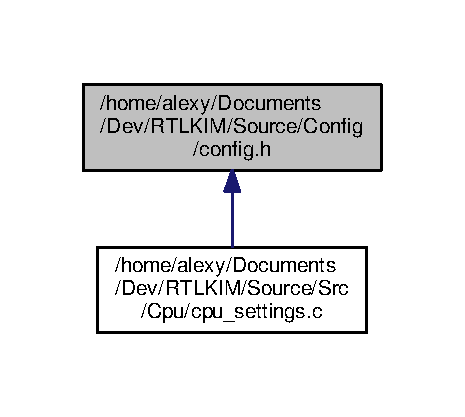
\includegraphics[width=223pt]{config_8h__dep__incl}
\end{center}
\end{figure}
\subsection*{Macros}
\begin{DoxyCompactItemize}
\item 
\#define \hyperlink{config_8h_a77383d4c5311d4c7fe49364766887650}{K\+E\+R\+N\+E\+L\+\_\+\+S\+T\+A\+C\+K\+\_\+\+S\+I\+ZE}~16384 /$\ast$ DO N\+OT F\+O\+R\+G\+ET TO M\+O\+D\+I\+FY IN L\+O\+A\+D\+E\+R.\+S $\ast$/
\item 
\#define \hyperlink{config_8h_add08506024a2c5399f9f9f6a797392ef}{M\+A\+X\+\_\+\+C\+P\+U\+\_\+\+C\+O\+U\+NT}~1
\item 
\#define \hyperlink{config_8h_a5cf9e6a54cccb394412952934ca25ef9}{E\+N\+A\+B\+L\+E\+\_\+\+S\+MP}~0
\item 
\#define \hyperlink{config_8h_a5b3722ea9a67e434cf9497dc440aba8b}{E\+N\+A\+B\+L\+E\+\_\+\+V\+E\+SA}~0
\item 
\#define \hyperlink{config_8h_af76715ead14e1dab3e4832d3bc3b56f2}{E\+N\+A\+B\+L\+E\+\_\+\+A\+TA}~0
\item 
\#define \hyperlink{config_8h_a601196b7b3fa93442b47a82c5ffcd677}{E\+N\+A\+B\+L\+E\+\_\+\+G\+UI}~0
\item 
\#define \hyperlink{config_8h_a618bdf461c25d552e654d6b899de2d37}{E\+N\+A\+B\+L\+E\+\_\+\+M\+O\+U\+SE}~0
\item 
\#define \hyperlink{config_8h_a8b77caaef5b34ab4a755236dd68ffc45}{M\+A\+X\+\_\+\+S\+U\+P\+P\+O\+R\+T\+E\+D\+\_\+\+H\+E\+I\+G\+HT}~1080
\item 
\#define \hyperlink{config_8h_a25c971d31e73490a7c3918b0cb3b6ef4}{M\+A\+X\+\_\+\+S\+U\+P\+P\+O\+R\+T\+E\+D\+\_\+\+W\+I\+D\+TH}~1100
\item 
\#define \hyperlink{config_8h_aae2b313893f4a2068c41e172d2091b80}{M\+A\+X\+\_\+\+S\+U\+P\+P\+O\+R\+T\+E\+D\+\_\+\+B\+PP}~32
\end{DoxyCompactItemize}


\subsection{Macro Definition Documentation}
\mbox{\Hypertarget{config_8h_af76715ead14e1dab3e4832d3bc3b56f2}\label{config_8h_af76715ead14e1dab3e4832d3bc3b56f2}} 
\index{config.\+h@{config.\+h}!E\+N\+A\+B\+L\+E\+\_\+\+A\+TA@{E\+N\+A\+B\+L\+E\+\_\+\+A\+TA}}
\index{E\+N\+A\+B\+L\+E\+\_\+\+A\+TA@{E\+N\+A\+B\+L\+E\+\_\+\+A\+TA}!config.\+h@{config.\+h}}
\subsubsection{\texorpdfstring{E\+N\+A\+B\+L\+E\+\_\+\+A\+TA}{ENABLE\_ATA}}
{\footnotesize\ttfamily \#define E\+N\+A\+B\+L\+E\+\_\+\+A\+TA~0}

\mbox{\Hypertarget{config_8h_a601196b7b3fa93442b47a82c5ffcd677}\label{config_8h_a601196b7b3fa93442b47a82c5ffcd677}} 
\index{config.\+h@{config.\+h}!E\+N\+A\+B\+L\+E\+\_\+\+G\+UI@{E\+N\+A\+B\+L\+E\+\_\+\+G\+UI}}
\index{E\+N\+A\+B\+L\+E\+\_\+\+G\+UI@{E\+N\+A\+B\+L\+E\+\_\+\+G\+UI}!config.\+h@{config.\+h}}
\subsubsection{\texorpdfstring{E\+N\+A\+B\+L\+E\+\_\+\+G\+UI}{ENABLE\_GUI}}
{\footnotesize\ttfamily \#define E\+N\+A\+B\+L\+E\+\_\+\+G\+UI~0}

\mbox{\Hypertarget{config_8h_a618bdf461c25d552e654d6b899de2d37}\label{config_8h_a618bdf461c25d552e654d6b899de2d37}} 
\index{config.\+h@{config.\+h}!E\+N\+A\+B\+L\+E\+\_\+\+M\+O\+U\+SE@{E\+N\+A\+B\+L\+E\+\_\+\+M\+O\+U\+SE}}
\index{E\+N\+A\+B\+L\+E\+\_\+\+M\+O\+U\+SE@{E\+N\+A\+B\+L\+E\+\_\+\+M\+O\+U\+SE}!config.\+h@{config.\+h}}
\subsubsection{\texorpdfstring{E\+N\+A\+B\+L\+E\+\_\+\+M\+O\+U\+SE}{ENABLE\_MOUSE}}
{\footnotesize\ttfamily \#define E\+N\+A\+B\+L\+E\+\_\+\+M\+O\+U\+SE~0}

\mbox{\Hypertarget{config_8h_a5cf9e6a54cccb394412952934ca25ef9}\label{config_8h_a5cf9e6a54cccb394412952934ca25ef9}} 
\index{config.\+h@{config.\+h}!E\+N\+A\+B\+L\+E\+\_\+\+S\+MP@{E\+N\+A\+B\+L\+E\+\_\+\+S\+MP}}
\index{E\+N\+A\+B\+L\+E\+\_\+\+S\+MP@{E\+N\+A\+B\+L\+E\+\_\+\+S\+MP}!config.\+h@{config.\+h}}
\subsubsection{\texorpdfstring{E\+N\+A\+B\+L\+E\+\_\+\+S\+MP}{ENABLE\_SMP}}
{\footnotesize\ttfamily \#define E\+N\+A\+B\+L\+E\+\_\+\+S\+MP~0}

\mbox{\Hypertarget{config_8h_a5b3722ea9a67e434cf9497dc440aba8b}\label{config_8h_a5b3722ea9a67e434cf9497dc440aba8b}} 
\index{config.\+h@{config.\+h}!E\+N\+A\+B\+L\+E\+\_\+\+V\+E\+SA@{E\+N\+A\+B\+L\+E\+\_\+\+V\+E\+SA}}
\index{E\+N\+A\+B\+L\+E\+\_\+\+V\+E\+SA@{E\+N\+A\+B\+L\+E\+\_\+\+V\+E\+SA}!config.\+h@{config.\+h}}
\subsubsection{\texorpdfstring{E\+N\+A\+B\+L\+E\+\_\+\+V\+E\+SA}{ENABLE\_VESA}}
{\footnotesize\ttfamily \#define E\+N\+A\+B\+L\+E\+\_\+\+V\+E\+SA~0}

\mbox{\Hypertarget{config_8h_a77383d4c5311d4c7fe49364766887650}\label{config_8h_a77383d4c5311d4c7fe49364766887650}} 
\index{config.\+h@{config.\+h}!K\+E\+R\+N\+E\+L\+\_\+\+S\+T\+A\+C\+K\+\_\+\+S\+I\+ZE@{K\+E\+R\+N\+E\+L\+\_\+\+S\+T\+A\+C\+K\+\_\+\+S\+I\+ZE}}
\index{K\+E\+R\+N\+E\+L\+\_\+\+S\+T\+A\+C\+K\+\_\+\+S\+I\+ZE@{K\+E\+R\+N\+E\+L\+\_\+\+S\+T\+A\+C\+K\+\_\+\+S\+I\+ZE}!config.\+h@{config.\+h}}
\subsubsection{\texorpdfstring{K\+E\+R\+N\+E\+L\+\_\+\+S\+T\+A\+C\+K\+\_\+\+S\+I\+ZE}{KERNEL\_STACK\_SIZE}}
{\footnotesize\ttfamily \#define K\+E\+R\+N\+E\+L\+\_\+\+S\+T\+A\+C\+K\+\_\+\+S\+I\+ZE~16384 /$\ast$ DO N\+OT F\+O\+R\+G\+ET TO M\+O\+D\+I\+FY IN L\+O\+A\+D\+E\+R.\+S $\ast$/}

\mbox{\Hypertarget{config_8h_add08506024a2c5399f9f9f6a797392ef}\label{config_8h_add08506024a2c5399f9f9f6a797392ef}} 
\index{config.\+h@{config.\+h}!M\+A\+X\+\_\+\+C\+P\+U\+\_\+\+C\+O\+U\+NT@{M\+A\+X\+\_\+\+C\+P\+U\+\_\+\+C\+O\+U\+NT}}
\index{M\+A\+X\+\_\+\+C\+P\+U\+\_\+\+C\+O\+U\+NT@{M\+A\+X\+\_\+\+C\+P\+U\+\_\+\+C\+O\+U\+NT}!config.\+h@{config.\+h}}
\subsubsection{\texorpdfstring{M\+A\+X\+\_\+\+C\+P\+U\+\_\+\+C\+O\+U\+NT}{MAX\_CPU\_COUNT}}
{\footnotesize\ttfamily \#define M\+A\+X\+\_\+\+C\+P\+U\+\_\+\+C\+O\+U\+NT~1}

\mbox{\Hypertarget{config_8h_aae2b313893f4a2068c41e172d2091b80}\label{config_8h_aae2b313893f4a2068c41e172d2091b80}} 
\index{config.\+h@{config.\+h}!M\+A\+X\+\_\+\+S\+U\+P\+P\+O\+R\+T\+E\+D\+\_\+\+B\+PP@{M\+A\+X\+\_\+\+S\+U\+P\+P\+O\+R\+T\+E\+D\+\_\+\+B\+PP}}
\index{M\+A\+X\+\_\+\+S\+U\+P\+P\+O\+R\+T\+E\+D\+\_\+\+B\+PP@{M\+A\+X\+\_\+\+S\+U\+P\+P\+O\+R\+T\+E\+D\+\_\+\+B\+PP}!config.\+h@{config.\+h}}
\subsubsection{\texorpdfstring{M\+A\+X\+\_\+\+S\+U\+P\+P\+O\+R\+T\+E\+D\+\_\+\+B\+PP}{MAX\_SUPPORTED\_BPP}}
{\footnotesize\ttfamily \#define M\+A\+X\+\_\+\+S\+U\+P\+P\+O\+R\+T\+E\+D\+\_\+\+B\+PP~32}

\mbox{\Hypertarget{config_8h_a8b77caaef5b34ab4a755236dd68ffc45}\label{config_8h_a8b77caaef5b34ab4a755236dd68ffc45}} 
\index{config.\+h@{config.\+h}!M\+A\+X\+\_\+\+S\+U\+P\+P\+O\+R\+T\+E\+D\+\_\+\+H\+E\+I\+G\+HT@{M\+A\+X\+\_\+\+S\+U\+P\+P\+O\+R\+T\+E\+D\+\_\+\+H\+E\+I\+G\+HT}}
\index{M\+A\+X\+\_\+\+S\+U\+P\+P\+O\+R\+T\+E\+D\+\_\+\+H\+E\+I\+G\+HT@{M\+A\+X\+\_\+\+S\+U\+P\+P\+O\+R\+T\+E\+D\+\_\+\+H\+E\+I\+G\+HT}!config.\+h@{config.\+h}}
\subsubsection{\texorpdfstring{M\+A\+X\+\_\+\+S\+U\+P\+P\+O\+R\+T\+E\+D\+\_\+\+H\+E\+I\+G\+HT}{MAX\_SUPPORTED\_HEIGHT}}
{\footnotesize\ttfamily \#define M\+A\+X\+\_\+\+S\+U\+P\+P\+O\+R\+T\+E\+D\+\_\+\+H\+E\+I\+G\+HT~1080}

\mbox{\Hypertarget{config_8h_a25c971d31e73490a7c3918b0cb3b6ef4}\label{config_8h_a25c971d31e73490a7c3918b0cb3b6ef4}} 
\index{config.\+h@{config.\+h}!M\+A\+X\+\_\+\+S\+U\+P\+P\+O\+R\+T\+E\+D\+\_\+\+W\+I\+D\+TH@{M\+A\+X\+\_\+\+S\+U\+P\+P\+O\+R\+T\+E\+D\+\_\+\+W\+I\+D\+TH}}
\index{M\+A\+X\+\_\+\+S\+U\+P\+P\+O\+R\+T\+E\+D\+\_\+\+W\+I\+D\+TH@{M\+A\+X\+\_\+\+S\+U\+P\+P\+O\+R\+T\+E\+D\+\_\+\+W\+I\+D\+TH}!config.\+h@{config.\+h}}
\subsubsection{\texorpdfstring{M\+A\+X\+\_\+\+S\+U\+P\+P\+O\+R\+T\+E\+D\+\_\+\+W\+I\+D\+TH}{MAX\_SUPPORTED\_WIDTH}}
{\footnotesize\ttfamily \#define M\+A\+X\+\_\+\+S\+U\+P\+P\+O\+R\+T\+E\+D\+\_\+\+W\+I\+D\+TH~1100}


\hypertarget{cpu_8h}{}\section{/home/alexy/\+Documents/\+Dev/\+R\+T\+L\+K\+I\+M/\+Source/\+Includes/\+Cpu/cpu.h File Reference}
\label{cpu_8h}\index{/home/alexy/\+Documents/\+Dev/\+R\+T\+L\+K\+I\+M/\+Source/\+Includes/\+Cpu/cpu.\+h@{/home/alexy/\+Documents/\+Dev/\+R\+T\+L\+K\+I\+M/\+Source/\+Includes/\+Cpu/cpu.\+h}}
{\ttfamily \#include $<$Lib/stdint.\+h$>$}\newline
{\ttfamily \#include $<$Lib/stddef.\+h$>$}\newline
Include dependency graph for cpu.\+h\+:\nopagebreak
\begin{figure}[H]
\begin{center}
\leavevmode
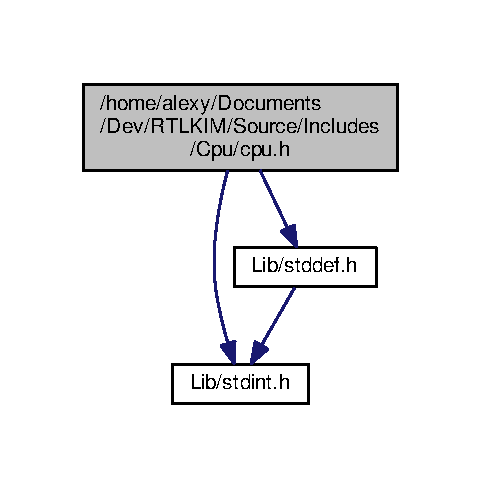
\includegraphics[width=231pt]{cpu_8h__incl}
\end{center}
\end{figure}
This graph shows which files directly or indirectly include this file\+:\nopagebreak
\begin{figure}[H]
\begin{center}
\leavevmode
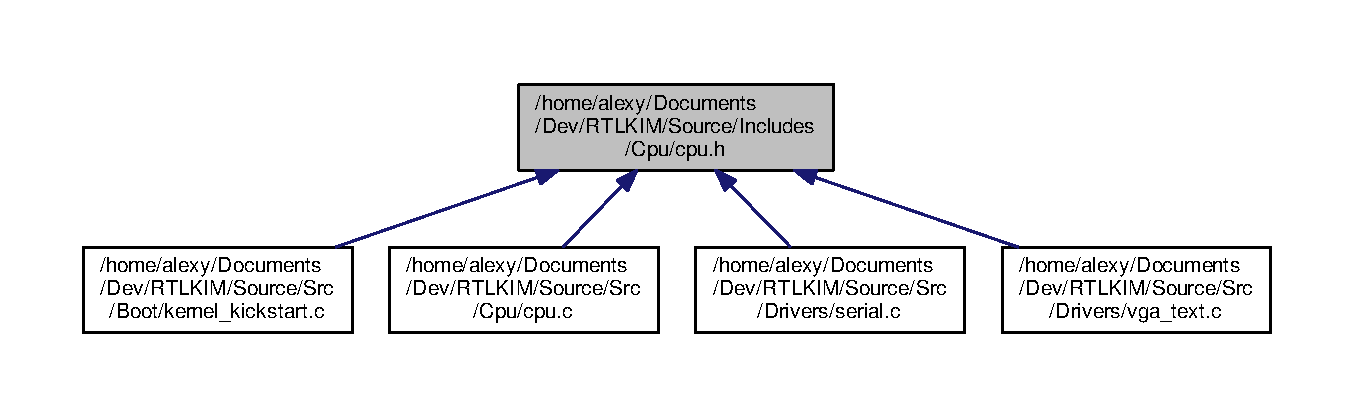
\includegraphics[width=350pt]{cpu_8h__dep__incl}
\end{center}
\end{figure}
\subsection*{Data Structures}
\begin{DoxyCompactItemize}
\item 
struct \hyperlink{structcpu__info}{cpu\+\_\+info}
\end{DoxyCompactItemize}
\subsection*{Macros}
\begin{DoxyCompactItemize}
\item 
\#define \hyperlink{cpu_8h_a9a98dd1b48b143c627b492fc337ed6c1}{C\+P\+U\+\_\+\+F\+L\+A\+G\+\_\+\+C\+P\+U\+I\+D\+\_\+\+C\+A\+P\+A\+B\+LE}~0x00200000
\item 
\#define \hyperlink{cpu_8h_aea40363130ccd9d4c7e89aa737f73928}{E\+C\+X\+\_\+\+S\+S\+E3}~(1 $<$$<$ 0)    /$\ast$ Streaming S\+I\+MD Extensions 3 $\ast$/
\item 
\#define \hyperlink{cpu_8h_a88006299e38c976b1eb1576f5f0508fe}{E\+C\+X\+\_\+\+P\+C\+L\+M\+U\+L\+Q\+DQ}~(1 $<$$<$ 1)    /$\ast$ P\+C\+L\+M\+U\+L\+Q\+DQ Instruction $\ast$/
\item 
\#define \hyperlink{cpu_8h_a2f0e06cb94d0e0c3f2bab3f8c6d1863f}{E\+C\+X\+\_\+\+D\+T\+E\+S64}~(1 $<$$<$ 2)    /$\ast$ 64-\/Bit Debug Store Area $\ast$/
\item 
\#define \hyperlink{cpu_8h_a27146cfe684acf96c9817eff2d1d1027}{E\+C\+X\+\_\+\+M\+O\+N\+I\+T\+OR}~(1 $<$$<$ 3)    /$\ast$ M\+O\+N\+I\+T\+OR/M\+W\+A\+IT $\ast$/
\item 
\#define \hyperlink{cpu_8h_a99e3f2da1d8254e07b318ac9e707af19}{E\+C\+X\+\_\+\+D\+S\+\_\+\+C\+PL}~(1 $<$$<$ 4)    /$\ast$ C\+PL Qualified Debug Store $\ast$/
\item 
\#define \hyperlink{cpu_8h_aed75bfda2658ce0abde52516068e8dec}{E\+C\+X\+\_\+\+V\+MX}~(1 $<$$<$ 5)    /$\ast$ Virtual Machine Extensions $\ast$/
\item 
\#define \hyperlink{cpu_8h_afcb5019b5501e71a85eb19e50dc6937d}{E\+C\+X\+\_\+\+S\+MX}~(1 $<$$<$ 6)    /$\ast$ Safer Mode Extensions $\ast$/
\item 
\#define \hyperlink{cpu_8h_a867c000609c5cab333cfe7fdec00da2d}{E\+C\+X\+\_\+\+E\+ST}~(1 $<$$<$ 7)    /$\ast$ Enhanced Speed\+Step Technology $\ast$/
\item 
\#define \hyperlink{cpu_8h_ade524e9bdbe9bcbc9e5891520fd90bc8}{E\+C\+X\+\_\+\+T\+M2}~(1 $<$$<$ 8)    /$\ast$ Thermal Monitor 2 $\ast$/
\item 
\#define \hyperlink{cpu_8h_adead9f0882ae71eaa184683013c29c09}{E\+C\+X\+\_\+\+S\+S\+S\+E3}~(1 $<$$<$ 9)    /$\ast$ Supplemental Streaming S\+I\+MD Extensions 3 $\ast$/
\item 
\#define \hyperlink{cpu_8h_a7ce8b2a030b99c9b238d494aa758edb4}{E\+C\+X\+\_\+\+C\+N\+X\+T\+\_\+\+ID}~(1 $<$$<$ 10)   /$\ast$ L1 Context ID $\ast$/
\item 
\#define \hyperlink{cpu_8h_ac8670a3a65aa96e663591d9f277eaccd}{E\+C\+X\+\_\+\+F\+MA}~(1 $<$$<$ 12)   /$\ast$ Fused Multiply Add $\ast$/
\item 
\#define \hyperlink{cpu_8h_a773e7f78a4a9bb86e99a27501c79f6fc}{E\+C\+X\+\_\+\+C\+X16}~(1 $<$$<$ 13)   /$\ast$ C\+M\+P\+X\+C\+H\+G16B Instruction $\ast$/
\item 
\#define \hyperlink{cpu_8h_aa907c0beedeb79202076709d4bb09cac}{E\+C\+X\+\_\+\+X\+T\+PR}~(1 $<$$<$ 14)   /$\ast$ x\+T\+PR Update Control $\ast$/
\item 
\#define \hyperlink{cpu_8h_aa87a6cf2cf7e0b63b2630873e46894db}{E\+C\+X\+\_\+\+P\+D\+CM}~(1 $<$$<$ 15)   /$\ast$ Perf/Debug Capability M\+SR $\ast$/
\item 
\#define \hyperlink{cpu_8h_a947bf94a2d4a994827fd10caeb2527e3}{E\+C\+X\+\_\+\+P\+C\+ID}~(1 $<$$<$ 17)   /$\ast$ Process-\/context Identifiers $\ast$/
\item 
\#define \hyperlink{cpu_8h_aade9b84e1aa8231731065de50a865bb4}{E\+C\+X\+\_\+\+D\+CA}~(1 $<$$<$ 18)   /$\ast$ Direct Cache Access $\ast$/
\item 
\#define \hyperlink{cpu_8h_a910c539f21ccd254628ade665ddfb1ab}{E\+C\+X\+\_\+\+S\+S\+E41}~(1 $<$$<$ 19)   /$\ast$ Streaming S\+I\+MD Extensions 4.\+1 $\ast$/
\item 
\#define \hyperlink{cpu_8h_a10db7841963e9f64b870ea960e27cd51}{E\+C\+X\+\_\+\+S\+S\+E42}~(1 $<$$<$ 20)   /$\ast$ Streaming S\+I\+MD Extensions 4.\+2 $\ast$/
\item 
\#define \hyperlink{cpu_8h_a8c5ff002801115c449bf38cd4abad370}{E\+C\+X\+\_\+\+X2\+A\+P\+IC}~(1 $<$$<$ 21)   /$\ast$ Extended x\+A\+P\+IC Support $\ast$/
\item 
\#define \hyperlink{cpu_8h_a673d46b999e2039c8eab155deba2795b}{E\+C\+X\+\_\+\+M\+O\+V\+BE}~(1 $<$$<$ 22)   /$\ast$ M\+O\+V\+BE Instruction $\ast$/
\item 
\#define \hyperlink{cpu_8h_a9fa42d78070f22e934f5f3008c5aa49f}{E\+C\+X\+\_\+\+P\+O\+P\+C\+NT}~(1 $<$$<$ 23)   /$\ast$ P\+O\+P\+C\+NT Instruction $\ast$/
\item 
\#define \hyperlink{cpu_8h_abea85010fe030520df7caa50eb1713b0}{E\+C\+X\+\_\+\+T\+SC}~(1 $<$$<$ 24)   /$\ast$ Local A\+P\+IC supports T\+SC Deadline $\ast$/
\item 
\#define \hyperlink{cpu_8h_a392a5490e1de75744ac9e15b2b1e2f10}{E\+C\+X\+\_\+\+A\+E\+S\+NI}~(1 $<$$<$ 25)   /$\ast$ A\+E\+S\+NI Instruction $\ast$/
\item 
\#define \hyperlink{cpu_8h_ac8bb9abac5611dd05d00482be7c9e808}{E\+C\+X\+\_\+\+X\+S\+A\+VE}~(1 $<$$<$ 26)   /$\ast$ X\+S\+A\+VE/X\+S\+T\+OR States $\ast$/
\item 
\#define \hyperlink{cpu_8h_abb62a3cd9d14bbad65660cb66fd42d81}{E\+C\+X\+\_\+\+O\+S\+X\+S\+A\+VE}~(1 $<$$<$ 27)   /$\ast$ OS Enabled Extended State Management $\ast$/
\item 
\#define \hyperlink{cpu_8h_a9dd4cf8905dae4fd3e5a8fbeec714a78}{E\+C\+X\+\_\+\+A\+VX}~(1 $<$$<$ 28)   /$\ast$ A\+VX Instructions $\ast$/
\item 
\#define \hyperlink{cpu_8h_a493b67200dada6ff6748e64fc59b51ea}{E\+C\+X\+\_\+\+F16C}~(1 $<$$<$ 29)   /$\ast$ 16-\/bit Floating Point Instructions $\ast$/
\item 
\#define \hyperlink{cpu_8h_a43ed2edda144fb065a33af72cb74708d}{E\+C\+X\+\_\+\+R\+D\+R\+A\+ND}~(1 $<$$<$ 30)   /$\ast$ R\+D\+R\+A\+ND Instruction $\ast$/
\item 
\#define \hyperlink{cpu_8h_a8b0ef1551723fe0271392495d155f9ed}{E\+D\+X\+\_\+\+F\+PU}~(1 $<$$<$ 0)    /$\ast$ Floating-\/Point Unit On-\/Chip $\ast$/
\item 
\#define \hyperlink{cpu_8h_ae09b05a6f9ea9cd8491705aa5a24a6fa}{E\+D\+X\+\_\+\+V\+ME}~(1 $<$$<$ 1)    /$\ast$ Virtual 8086 Mode Extensions $\ast$/
\item 
\#define \hyperlink{cpu_8h_a3ffb4c68958b1a27682f3e86cb8756dc}{E\+D\+X\+\_\+\+DE}~(1 $<$$<$ 2)    /$\ast$ Debugging Extensions $\ast$/
\item 
\#define \hyperlink{cpu_8h_a788411e5452e502dc20fcacdf4799ccb}{E\+D\+X\+\_\+\+P\+SE}~(1 $<$$<$ 3)    /$\ast$ Page Size Extension $\ast$/
\item 
\#define \hyperlink{cpu_8h_ab6ab73c8dc4cf7f6d6b24800d7991f3a}{E\+D\+X\+\_\+\+T\+SC}~(1 $<$$<$ 4)    /$\ast$ Time Stamp Counter $\ast$/
\item 
\#define \hyperlink{cpu_8h_aea31f6d48e27d721488c9237dc82a8ec}{E\+D\+X\+\_\+\+M\+SR}~(1 $<$$<$ 5)    /$\ast$ Model Specific Registers $\ast$/
\item 
\#define \hyperlink{cpu_8h_aeef18667596f1d5f295ba641b84aea16}{E\+D\+X\+\_\+\+P\+AE}~(1 $<$$<$ 6)    /$\ast$ Physical Address Extension $\ast$/
\item 
\#define \hyperlink{cpu_8h_ab3ec694ce4542e0458eaaf2769b44537}{E\+D\+X\+\_\+\+M\+CE}~(1 $<$$<$ 7)    /$\ast$ Machine-\/Check Exception $\ast$/
\item 
\#define \hyperlink{cpu_8h_aad35b13967c9a0ab20179509fcd19ae1}{E\+D\+X\+\_\+\+C\+X8}~(1 $<$$<$ 8)    /$\ast$ C\+M\+P\+X\+C\+H\+G8 Instruction $\ast$/
\item 
\#define \hyperlink{cpu_8h_ad8410aec38ee96c662f35fba3c5ef16b}{E\+D\+X\+\_\+\+A\+P\+IC}~(1 $<$$<$ 9)    /$\ast$ A\+P\+IC On-\/Chip $\ast$/
\item 
\#define \hyperlink{cpu_8h_a540c4fc3352a42253fe3c942f118306e}{E\+D\+X\+\_\+\+S\+EP}~(1 $<$$<$ 11)   /$\ast$ S\+Y\+S\+E\+N\+T\+ER/S\+Y\+S\+E\+X\+IT instructions $\ast$/
\item 
\#define \hyperlink{cpu_8h_a5b0e55fb245f2e2de587822d934d71d5}{E\+D\+X\+\_\+\+M\+T\+RR}~(1 $<$$<$ 12)   /$\ast$ Memory Type Range Registers $\ast$/
\item 
\#define \hyperlink{cpu_8h_a73d42efffc1c0de0fc011d5a8c905e84}{E\+D\+X\+\_\+\+P\+GE}~(1 $<$$<$ 13)   /$\ast$ Page Global Bit $\ast$/
\item 
\#define \hyperlink{cpu_8h_a2c09c3f6eefb2a1ebea5a9d504b48ae2}{E\+D\+X\+\_\+\+M\+CA}~(1 $<$$<$ 14)   /$\ast$ Machine-\/Check Architecture $\ast$/
\item 
\#define \hyperlink{cpu_8h_a12c3d2ed0a9654f54765a9e7460da598}{E\+D\+X\+\_\+\+C\+M\+OV}~(1 $<$$<$ 15)   /$\ast$ Conditional Move Instruction $\ast$/
\item 
\#define \hyperlink{cpu_8h_ac5144147c0a6a325b093e7085f65bceb}{E\+D\+X\+\_\+\+P\+AT}~(1 $<$$<$ 16)   /$\ast$ Page Attribute Table $\ast$/
\item 
\#define \hyperlink{cpu_8h_a95daa6db40e5e4ead4580d776415f239}{E\+D\+X\+\_\+\+P\+S\+E36}~(1 $<$$<$ 17)   /$\ast$ 36-\/bit Page Size Extension $\ast$/
\item 
\#define \hyperlink{cpu_8h_a2cad8344c1fde4647d3296482da57a1a}{E\+D\+X\+\_\+\+P\+SN}~(1 $<$$<$ 18)   /$\ast$ Processor Serial Number $\ast$/
\item 
\#define \hyperlink{cpu_8h_a6273a34177b8c2eb9f5c77a15d1bd42f}{E\+D\+X\+\_\+\+C\+L\+F\+L\+U\+SH}~(1 $<$$<$ 19)   /$\ast$ C\+L\+F\+L\+U\+SH Instruction $\ast$/
\item 
\#define \hyperlink{cpu_8h_a4a6797d78f8ff5e2faed04e3fdd49d66}{E\+D\+X\+\_\+\+DS}~(1 $<$$<$ 21)   /$\ast$ Debug Store $\ast$/
\item 
\#define \hyperlink{cpu_8h_a5e42f48d8327853ac9946239b5078f19}{E\+D\+X\+\_\+\+A\+C\+PI}~(1 $<$$<$ 22)   /$\ast$ Thermal Monitor and Clock Facilities $\ast$/
\item 
\#define \hyperlink{cpu_8h_a3a3ef54ca6bc42f3e4815c5c10b66e41}{E\+D\+X\+\_\+\+M\+MX}~(1 $<$$<$ 23)   /$\ast$ M\+MX Technology $\ast$/
\item 
\#define \hyperlink{cpu_8h_a8153a684e9964ae00247a4ca5fd2a22e}{E\+D\+X\+\_\+\+F\+X\+SR}~(1 $<$$<$ 24)   /$\ast$ F\+X\+S\+A\+VE and F\+X\+S\+T\+OR Instructions $\ast$/
\item 
\#define \hyperlink{cpu_8h_a1556ce3fb2d89acf7980d369f7ab7d89}{E\+D\+X\+\_\+\+S\+SE}~(1 $<$$<$ 25)   /$\ast$ Streaming S\+I\+MD Extensions $\ast$/
\item 
\#define \hyperlink{cpu_8h_a2c4a6c8eacee56abaf7f7010ae619a4b}{E\+D\+X\+\_\+\+S\+S\+E2}~(1 $<$$<$ 26)   /$\ast$ Streaming S\+I\+MD Extensions 2 $\ast$/
\item 
\#define \hyperlink{cpu_8h_adfaf379e276c5129dda2cab7e70846ef}{E\+D\+X\+\_\+\+SS}~(1 $<$$<$ 27)   /$\ast$ Self Snoop $\ast$/
\item 
\#define \hyperlink{cpu_8h_a36c3ca3dc06f341d7b115d20e0764eb2}{E\+D\+X\+\_\+\+H\+TT}~(1 $<$$<$ 28)   /$\ast$ Multi-\/Threading $\ast$/
\item 
\#define \hyperlink{cpu_8h_a89de2f3104e154abe2d289115ef60826}{E\+D\+X\+\_\+\+TM}~(1 $<$$<$ 29)   /$\ast$ Thermal Monitor $\ast$/
\item 
\#define \hyperlink{cpu_8h_ab25d114021d91efd3861dd1edab22b00}{E\+D\+X\+\_\+\+P\+BE}~(1 $<$$<$ 31)   /$\ast$ Pending Break Enable $\ast$/
\item 
\#define \hyperlink{cpu_8h_a818a32e2d1996dd7c79ae06d3aa4c6b6}{E\+D\+X\+\_\+\+S\+Y\+S\+C\+A\+LL}~(1 $<$$<$ 11)   /$\ast$ S\+Y\+S\+C\+A\+LL/S\+Y\+S\+R\+ET $\ast$/
\item 
\#define \hyperlink{cpu_8h_a6f8e81fc64a30bc76f7b477629d130cf}{E\+D\+X\+\_\+\+XD}~(1 $<$$<$ 20)   /$\ast$ Execute Disable Bit $\ast$/
\item 
\#define \hyperlink{cpu_8h_ade94ed02d5475ab6008229944b594dd0}{E\+D\+X\+\_\+1\+G\+B\+\_\+\+P\+A\+GE}~(1 $<$$<$ 26)   /$\ast$ 1 GB Pages $\ast$/
\item 
\#define \hyperlink{cpu_8h_a0cb3f8b38750485ac9715dcfbc407b9b}{E\+D\+X\+\_\+\+R\+D\+T\+S\+CP}~(1 $<$$<$ 27)   /$\ast$ R\+D\+T\+S\+CP and I\+A32\+\_\+\+T\+S\+C\+\_\+\+A\+UX $\ast$/
\item 
\#define \hyperlink{cpu_8h_a6fad8a7de471fcd3e77bdecdff29985b}{E\+D\+X\+\_\+64\+\_\+\+B\+IT}~(1 $<$$<$ 29)   /$\ast$ 64-\/bit Architecture $\ast$/
\item 
\#define \hyperlink{cpu_8h_a0915f239ce43398abcbb4f45335e5f10}{S\+I\+G\+\_\+\+A\+M\+D\+\_\+\+E\+BX}~0x68747541
\item 
\#define \hyperlink{cpu_8h_a1794ea3e87a9cc307620f7595ba6bc98}{S\+I\+G\+\_\+\+A\+M\+D\+\_\+\+E\+CX}~0x444d4163
\item 
\#define \hyperlink{cpu_8h_ac825533e3242b18d4c5e2f5df572e07f}{S\+I\+G\+\_\+\+A\+M\+D\+\_\+\+E\+DX}~0x69746e65
\item 
\#define \hyperlink{cpu_8h_af46afc0c5bcd1f614898e48c2904bb35}{S\+I\+G\+\_\+\+C\+E\+N\+T\+A\+U\+R\+\_\+\+E\+BX}~0x746e6543
\item 
\#define \hyperlink{cpu_8h_a4ec5ac45ae7da1bcb8612a9fa4750e15}{S\+I\+G\+\_\+\+C\+E\+N\+T\+A\+U\+R\+\_\+\+E\+CX}~0x736c7561
\item 
\#define \hyperlink{cpu_8h_ac3e504fe60f2cefb944949a7e7583517}{S\+I\+G\+\_\+\+C\+E\+N\+T\+A\+U\+R\+\_\+\+E\+DX}~0x48727561
\item 
\#define \hyperlink{cpu_8h_a8572734c594011bdbaa4dcea0ba32790}{S\+I\+G\+\_\+\+C\+Y\+R\+I\+X\+\_\+\+E\+BX}~0x69727943
\item 
\#define \hyperlink{cpu_8h_a29b2f5ab3f7ce067e89629f446e9f833}{S\+I\+G\+\_\+\+C\+Y\+R\+I\+X\+\_\+\+E\+CX}~0x64616574
\item 
\#define \hyperlink{cpu_8h_a9339d91116ccc31542692db4c2687aba}{S\+I\+G\+\_\+\+C\+Y\+R\+I\+X\+\_\+\+E\+DX}~0x736e4978
\item 
\#define \hyperlink{cpu_8h_a2e244c832675fe61c0ebd8502eb092f9}{S\+I\+G\+\_\+\+I\+N\+T\+E\+L\+\_\+\+E\+BX}~0x756e6547
\item 
\#define \hyperlink{cpu_8h_adcb4d2306514e8fa402cc9ea32ed2c04}{S\+I\+G\+\_\+\+I\+N\+T\+E\+L\+\_\+\+E\+CX}~0x6c65746e
\item 
\#define \hyperlink{cpu_8h_aefb4f8fa65f9ab024e41ed6d709719f7}{S\+I\+G\+\_\+\+I\+N\+T\+E\+L\+\_\+\+E\+DX}~0x49656e69
\item 
\#define \hyperlink{cpu_8h_a51e4f214d063e677c63e5d5a70c0d61f}{S\+I\+G\+\_\+\+T\+M1\+\_\+\+E\+BX}~0x6e617254
\item 
\#define \hyperlink{cpu_8h_a5c0810a91602a4f367054805485fc6ba}{S\+I\+G\+\_\+\+T\+M1\+\_\+\+E\+CX}~0x55504361
\item 
\#define \hyperlink{cpu_8h_a74243a8672945df4b8946bcb469586ee}{S\+I\+G\+\_\+\+T\+M1\+\_\+\+E\+DX}~0x74656d73
\item 
\#define \hyperlink{cpu_8h_a4aaabe82282bce2844ee8c1d7f24072c}{S\+I\+G\+\_\+\+T\+M2\+\_\+\+E\+BX}~0x756e6547
\item 
\#define \hyperlink{cpu_8h_a7704376775ad1b50a648fdd300ce3126}{S\+I\+G\+\_\+\+T\+M2\+\_\+\+E\+CX}~0x3638784d
\item 
\#define \hyperlink{cpu_8h_ab578d56a39ef3c481a9406acc446d931}{S\+I\+G\+\_\+\+T\+M2\+\_\+\+E\+DX}~0x54656e69
\item 
\#define \hyperlink{cpu_8h_aaaa6b845a3c69314bd13db13116dc074}{S\+I\+G\+\_\+\+N\+S\+C\+\_\+\+E\+BX}~0x646f6547
\item 
\#define \hyperlink{cpu_8h_aaa43d1b675582f622e3c9e52bcbbe820}{S\+I\+G\+\_\+\+N\+S\+C\+\_\+\+E\+CX}~0x43534e20
\item 
\#define \hyperlink{cpu_8h_a2d38b34c4e545bc7f6378e4e03a168a1}{S\+I\+G\+\_\+\+N\+S\+C\+\_\+\+E\+DX}~0x79622065
\item 
\#define \hyperlink{cpu_8h_a6ec08042c7ae70b152157e3542bc4fa4}{S\+I\+G\+\_\+\+N\+E\+X\+G\+E\+N\+\_\+\+E\+BX}~0x4778654e
\item 
\#define \hyperlink{cpu_8h_a0718b25b7ac07b54a912b42eccf2f81e}{S\+I\+G\+\_\+\+N\+E\+X\+G\+E\+N\+\_\+\+E\+CX}~0x6e657669
\item 
\#define \hyperlink{cpu_8h_a80f3b08dfa5392d2ea195f06da17af26}{S\+I\+G\+\_\+\+N\+E\+X\+G\+E\+N\+\_\+\+E\+DX}~0x72446e65
\item 
\#define \hyperlink{cpu_8h_a0f5ca43f20e8b90d7f56ef758a962576}{S\+I\+G\+\_\+\+R\+I\+S\+E\+\_\+\+E\+BX}~0x65736952
\item 
\#define \hyperlink{cpu_8h_ab5063e8e2b189c529a98d383231661a9}{S\+I\+G\+\_\+\+R\+I\+S\+E\+\_\+\+E\+CX}~0x65736952
\item 
\#define \hyperlink{cpu_8h_aabfb2b6f1c8a955a66771e88207f4fca}{S\+I\+G\+\_\+\+R\+I\+S\+E\+\_\+\+E\+DX}~0x65736952
\item 
\#define \hyperlink{cpu_8h_a95e35dc6bc612ed3ca2b62d96aad4490}{S\+I\+G\+\_\+\+S\+I\+S\+\_\+\+E\+BX}~0x20536953
\item 
\#define \hyperlink{cpu_8h_a019acd9668c47aaade8459cf02bbc53b}{S\+I\+G\+\_\+\+S\+I\+S\+\_\+\+E\+CX}~0x20536953
\item 
\#define \hyperlink{cpu_8h_aa0f0ea1cd406cb021b0072bf4557330f}{S\+I\+G\+\_\+\+S\+I\+S\+\_\+\+E\+DX}~0x20536953
\item 
\#define \hyperlink{cpu_8h_a74f1fcab89e99dd5a0c54d9c09ce125a}{S\+I\+G\+\_\+\+U\+M\+C\+\_\+\+E\+BX}~0x20434d55
\item 
\#define \hyperlink{cpu_8h_a58eaa0eb49655a460b320fe24ce485e3}{S\+I\+G\+\_\+\+U\+M\+C\+\_\+\+E\+CX}~0x20434d55
\item 
\#define \hyperlink{cpu_8h_a8ed1c32332f26f85bf8b69760cbca8b7}{S\+I\+G\+\_\+\+U\+M\+C\+\_\+\+E\+DX}~0x20434d55
\item 
\#define \hyperlink{cpu_8h_ad190f8f2013e4fd49c2ae7ae3cdaa0a4}{S\+I\+G\+\_\+\+V\+I\+A\+\_\+\+E\+BX}~0x20414956
\item 
\#define \hyperlink{cpu_8h_a897153b15eb006d498bee6373def0247}{S\+I\+G\+\_\+\+V\+I\+A\+\_\+\+E\+CX}~0x20414956
\item 
\#define \hyperlink{cpu_8h_a336c84c1330f7b9658715d9c43a0903b}{S\+I\+G\+\_\+\+V\+I\+A\+\_\+\+E\+DX}~0x20414956
\item 
\#define \hyperlink{cpu_8h_a23e64d4fab9d3a16407af2df225c94b4}{S\+I\+G\+\_\+\+V\+O\+R\+T\+E\+X\+\_\+\+E\+BX}~0x74726f56
\item 
\#define \hyperlink{cpu_8h_a53e2ac92ff19b3635afa1d68ca1c02ed}{S\+I\+G\+\_\+\+V\+O\+R\+T\+E\+X\+\_\+\+E\+CX}~0x436f5320
\item 
\#define \hyperlink{cpu_8h_ac97b4b5e076a64b228edf12bcf8d9d2d}{S\+I\+G\+\_\+\+V\+O\+R\+T\+E\+X\+\_\+\+E\+DX}~0x36387865
\end{DoxyCompactItemize}
\subsection*{Typedefs}
\begin{DoxyCompactItemize}
\item 
typedef struct \hyperlink{structcpu__info}{cpu\+\_\+info} \hyperlink{cpu_8h_a5d0444e34676b8c836666095091ceb88}{cpu\+\_\+info\+\_\+t}
\item 
typedef enum \hyperlink{cpu_8h_ae79fa892c49bf77dd5e8fc53d18c57b5}{cpuid\+\_\+requests} \hyperlink{cpu_8h_af2b9e3cafbfa629db8a1c6a67ef1063a}{C\+P\+U\+I\+D\+\_\+\+R\+E\+Q\+\_\+E}
\end{DoxyCompactItemize}
\subsection*{Enumerations}
\begin{DoxyCompactItemize}
\item 
enum \hyperlink{cpu_8h_ae79fa892c49bf77dd5e8fc53d18c57b5}{cpuid\+\_\+requests} \{ \newline
\hyperlink{cpu_8h_ae79fa892c49bf77dd5e8fc53d18c57b5a287b9480159ff0790f83312fc0f35361}{C\+P\+U\+I\+D\+\_\+\+G\+E\+T\+V\+E\+N\+D\+O\+R\+S\+T\+R\+I\+NG}, 
\hyperlink{cpu_8h_ae79fa892c49bf77dd5e8fc53d18c57b5ae54d5cf464a4eaab14f5639ef57a5350}{C\+P\+U\+I\+D\+\_\+\+G\+E\+T\+F\+E\+A\+T\+U\+R\+ES}, 
\hyperlink{cpu_8h_ae79fa892c49bf77dd5e8fc53d18c57b5a1844360ad06974a69963618af9fd7721}{C\+P\+U\+I\+D\+\_\+\+G\+E\+T\+T\+LB}, 
\hyperlink{cpu_8h_ae79fa892c49bf77dd5e8fc53d18c57b5ad206c016f6b1bf979bab7c632a2daaa4}{C\+P\+U\+I\+D\+\_\+\+G\+E\+T\+S\+E\+R\+I\+AL}, 
\newline
\hyperlink{cpu_8h_ae79fa892c49bf77dd5e8fc53d18c57b5ab016d439747f36e0a2bdd34f8f26ecbe}{C\+P\+U\+I\+D\+\_\+\+I\+N\+T\+E\+L\+E\+X\+T\+E\+N\+D\+ED} =0x80000000, 
\hyperlink{cpu_8h_ae79fa892c49bf77dd5e8fc53d18c57b5a6b1682619d4f05d42499c280f74ba7d0}{C\+P\+U\+I\+D\+\_\+\+I\+N\+T\+E\+L\+F\+E\+A\+T\+U\+R\+ES}, 
\hyperlink{cpu_8h_ae79fa892c49bf77dd5e8fc53d18c57b5a898f490021383393edca0741e4a3b8df}{C\+P\+U\+I\+D\+\_\+\+I\+N\+T\+E\+L\+B\+R\+A\+N\+D\+S\+T\+R\+I\+NG}, 
\hyperlink{cpu_8h_ae79fa892c49bf77dd5e8fc53d18c57b5a8585bcaf7fb2b6c52217566488dc3739}{C\+P\+U\+I\+D\+\_\+\+I\+N\+T\+E\+L\+B\+R\+A\+N\+D\+S\+T\+R\+I\+N\+G\+M\+O\+RE}, 
\newline
\hyperlink{cpu_8h_ae79fa892c49bf77dd5e8fc53d18c57b5af0e6c842bda49527a246dd9c85d6da6a}{C\+P\+U\+I\+D\+\_\+\+I\+N\+T\+E\+L\+B\+R\+A\+N\+D\+S\+T\+R\+I\+N\+G\+E\+ND}
 \}
\end{DoxyCompactItemize}
\subsection*{Functions}
\begin{DoxyCompactItemize}
\item 
\hyperlink{stddef_8h_a51557cb52bbb9ee9d55aab5b9b16c3d0}{O\+S\+\_\+\+R\+E\+T\+U\+R\+N\+\_\+E} \hyperlink{cpu_8h_a161ae3250d5ebc057b2784b850564c42}{get\+\_\+cpu\+\_\+info} (\hyperlink{cpu_8h_a5d0444e34676b8c836666095091ceb88}{cpu\+\_\+info\+\_\+t} $\ast$info)
\item 
\hyperlink{stdint_8h_aef44329758059c91c76d334e8fc09700}{int8\+\_\+t} \hyperlink{cpu_8h_a1a8cb55ce40a2adb1636440c1c20413c}{cpuid\+\_\+capable} (void)
\item 
void \hyperlink{cpu_8h_aab96f38dab23a8fc333a33b99d3d7de9}{detect\+\_\+cpu} (void)
\end{DoxyCompactItemize}


\subsection{Macro Definition Documentation}
\mbox{\Hypertarget{cpu_8h_a9a98dd1b48b143c627b492fc337ed6c1}\label{cpu_8h_a9a98dd1b48b143c627b492fc337ed6c1}} 
\index{cpu.\+h@{cpu.\+h}!C\+P\+U\+\_\+\+F\+L\+A\+G\+\_\+\+C\+P\+U\+I\+D\+\_\+\+C\+A\+P\+A\+B\+LE@{C\+P\+U\+\_\+\+F\+L\+A\+G\+\_\+\+C\+P\+U\+I\+D\+\_\+\+C\+A\+P\+A\+B\+LE}}
\index{C\+P\+U\+\_\+\+F\+L\+A\+G\+\_\+\+C\+P\+U\+I\+D\+\_\+\+C\+A\+P\+A\+B\+LE@{C\+P\+U\+\_\+\+F\+L\+A\+G\+\_\+\+C\+P\+U\+I\+D\+\_\+\+C\+A\+P\+A\+B\+LE}!cpu.\+h@{cpu.\+h}}
\subsubsection{\texorpdfstring{C\+P\+U\+\_\+\+F\+L\+A\+G\+\_\+\+C\+P\+U\+I\+D\+\_\+\+C\+A\+P\+A\+B\+LE}{CPU\_FLAG\_CPUID\_CAPABLE}}
{\footnotesize\ttfamily \#define C\+P\+U\+\_\+\+F\+L\+A\+G\+\_\+\+C\+P\+U\+I\+D\+\_\+\+C\+A\+P\+A\+B\+LE~0x00200000}

\mbox{\Hypertarget{cpu_8h_a392a5490e1de75744ac9e15b2b1e2f10}\label{cpu_8h_a392a5490e1de75744ac9e15b2b1e2f10}} 
\index{cpu.\+h@{cpu.\+h}!E\+C\+X\+\_\+\+A\+E\+S\+NI@{E\+C\+X\+\_\+\+A\+E\+S\+NI}}
\index{E\+C\+X\+\_\+\+A\+E\+S\+NI@{E\+C\+X\+\_\+\+A\+E\+S\+NI}!cpu.\+h@{cpu.\+h}}
\subsubsection{\texorpdfstring{E\+C\+X\+\_\+\+A\+E\+S\+NI}{ECX\_AESNI}}
{\footnotesize\ttfamily \#define E\+C\+X\+\_\+\+A\+E\+S\+NI~(1 $<$$<$ 25)   /$\ast$ A\+E\+S\+NI Instruction $\ast$/}

\mbox{\Hypertarget{cpu_8h_a9dd4cf8905dae4fd3e5a8fbeec714a78}\label{cpu_8h_a9dd4cf8905dae4fd3e5a8fbeec714a78}} 
\index{cpu.\+h@{cpu.\+h}!E\+C\+X\+\_\+\+A\+VX@{E\+C\+X\+\_\+\+A\+VX}}
\index{E\+C\+X\+\_\+\+A\+VX@{E\+C\+X\+\_\+\+A\+VX}!cpu.\+h@{cpu.\+h}}
\subsubsection{\texorpdfstring{E\+C\+X\+\_\+\+A\+VX}{ECX\_AVX}}
{\footnotesize\ttfamily \#define E\+C\+X\+\_\+\+A\+VX~(1 $<$$<$ 28)   /$\ast$ A\+VX Instructions $\ast$/}

\mbox{\Hypertarget{cpu_8h_a7ce8b2a030b99c9b238d494aa758edb4}\label{cpu_8h_a7ce8b2a030b99c9b238d494aa758edb4}} 
\index{cpu.\+h@{cpu.\+h}!E\+C\+X\+\_\+\+C\+N\+X\+T\+\_\+\+ID@{E\+C\+X\+\_\+\+C\+N\+X\+T\+\_\+\+ID}}
\index{E\+C\+X\+\_\+\+C\+N\+X\+T\+\_\+\+ID@{E\+C\+X\+\_\+\+C\+N\+X\+T\+\_\+\+ID}!cpu.\+h@{cpu.\+h}}
\subsubsection{\texorpdfstring{E\+C\+X\+\_\+\+C\+N\+X\+T\+\_\+\+ID}{ECX\_CNXT\_ID}}
{\footnotesize\ttfamily \#define E\+C\+X\+\_\+\+C\+N\+X\+T\+\_\+\+ID~(1 $<$$<$ 10)   /$\ast$ L1 Context ID $\ast$/}

\mbox{\Hypertarget{cpu_8h_a773e7f78a4a9bb86e99a27501c79f6fc}\label{cpu_8h_a773e7f78a4a9bb86e99a27501c79f6fc}} 
\index{cpu.\+h@{cpu.\+h}!E\+C\+X\+\_\+\+C\+X16@{E\+C\+X\+\_\+\+C\+X16}}
\index{E\+C\+X\+\_\+\+C\+X16@{E\+C\+X\+\_\+\+C\+X16}!cpu.\+h@{cpu.\+h}}
\subsubsection{\texorpdfstring{E\+C\+X\+\_\+\+C\+X16}{ECX\_CX16}}
{\footnotesize\ttfamily \#define E\+C\+X\+\_\+\+C\+X16~(1 $<$$<$ 13)   /$\ast$ C\+M\+P\+X\+C\+H\+G16B Instruction $\ast$/}

\mbox{\Hypertarget{cpu_8h_aade9b84e1aa8231731065de50a865bb4}\label{cpu_8h_aade9b84e1aa8231731065de50a865bb4}} 
\index{cpu.\+h@{cpu.\+h}!E\+C\+X\+\_\+\+D\+CA@{E\+C\+X\+\_\+\+D\+CA}}
\index{E\+C\+X\+\_\+\+D\+CA@{E\+C\+X\+\_\+\+D\+CA}!cpu.\+h@{cpu.\+h}}
\subsubsection{\texorpdfstring{E\+C\+X\+\_\+\+D\+CA}{ECX\_DCA}}
{\footnotesize\ttfamily \#define E\+C\+X\+\_\+\+D\+CA~(1 $<$$<$ 18)   /$\ast$ Direct Cache Access $\ast$/}

\mbox{\Hypertarget{cpu_8h_a99e3f2da1d8254e07b318ac9e707af19}\label{cpu_8h_a99e3f2da1d8254e07b318ac9e707af19}} 
\index{cpu.\+h@{cpu.\+h}!E\+C\+X\+\_\+\+D\+S\+\_\+\+C\+PL@{E\+C\+X\+\_\+\+D\+S\+\_\+\+C\+PL}}
\index{E\+C\+X\+\_\+\+D\+S\+\_\+\+C\+PL@{E\+C\+X\+\_\+\+D\+S\+\_\+\+C\+PL}!cpu.\+h@{cpu.\+h}}
\subsubsection{\texorpdfstring{E\+C\+X\+\_\+\+D\+S\+\_\+\+C\+PL}{ECX\_DS\_CPL}}
{\footnotesize\ttfamily \#define E\+C\+X\+\_\+\+D\+S\+\_\+\+C\+PL~(1 $<$$<$ 4)    /$\ast$ C\+PL Qualified Debug Store $\ast$/}

\mbox{\Hypertarget{cpu_8h_a2f0e06cb94d0e0c3f2bab3f8c6d1863f}\label{cpu_8h_a2f0e06cb94d0e0c3f2bab3f8c6d1863f}} 
\index{cpu.\+h@{cpu.\+h}!E\+C\+X\+\_\+\+D\+T\+E\+S64@{E\+C\+X\+\_\+\+D\+T\+E\+S64}}
\index{E\+C\+X\+\_\+\+D\+T\+E\+S64@{E\+C\+X\+\_\+\+D\+T\+E\+S64}!cpu.\+h@{cpu.\+h}}
\subsubsection{\texorpdfstring{E\+C\+X\+\_\+\+D\+T\+E\+S64}{ECX\_DTES64}}
{\footnotesize\ttfamily \#define E\+C\+X\+\_\+\+D\+T\+E\+S64~(1 $<$$<$ 2)    /$\ast$ 64-\/Bit Debug Store Area $\ast$/}

\mbox{\Hypertarget{cpu_8h_a867c000609c5cab333cfe7fdec00da2d}\label{cpu_8h_a867c000609c5cab333cfe7fdec00da2d}} 
\index{cpu.\+h@{cpu.\+h}!E\+C\+X\+\_\+\+E\+ST@{E\+C\+X\+\_\+\+E\+ST}}
\index{E\+C\+X\+\_\+\+E\+ST@{E\+C\+X\+\_\+\+E\+ST}!cpu.\+h@{cpu.\+h}}
\subsubsection{\texorpdfstring{E\+C\+X\+\_\+\+E\+ST}{ECX\_EST}}
{\footnotesize\ttfamily \#define E\+C\+X\+\_\+\+E\+ST~(1 $<$$<$ 7)    /$\ast$ Enhanced Speed\+Step Technology $\ast$/}

\mbox{\Hypertarget{cpu_8h_a493b67200dada6ff6748e64fc59b51ea}\label{cpu_8h_a493b67200dada6ff6748e64fc59b51ea}} 
\index{cpu.\+h@{cpu.\+h}!E\+C\+X\+\_\+\+F16C@{E\+C\+X\+\_\+\+F16C}}
\index{E\+C\+X\+\_\+\+F16C@{E\+C\+X\+\_\+\+F16C}!cpu.\+h@{cpu.\+h}}
\subsubsection{\texorpdfstring{E\+C\+X\+\_\+\+F16C}{ECX\_F16C}}
{\footnotesize\ttfamily \#define E\+C\+X\+\_\+\+F16C~(1 $<$$<$ 29)   /$\ast$ 16-\/bit Floating Point Instructions $\ast$/}

\mbox{\Hypertarget{cpu_8h_ac8670a3a65aa96e663591d9f277eaccd}\label{cpu_8h_ac8670a3a65aa96e663591d9f277eaccd}} 
\index{cpu.\+h@{cpu.\+h}!E\+C\+X\+\_\+\+F\+MA@{E\+C\+X\+\_\+\+F\+MA}}
\index{E\+C\+X\+\_\+\+F\+MA@{E\+C\+X\+\_\+\+F\+MA}!cpu.\+h@{cpu.\+h}}
\subsubsection{\texorpdfstring{E\+C\+X\+\_\+\+F\+MA}{ECX\_FMA}}
{\footnotesize\ttfamily \#define E\+C\+X\+\_\+\+F\+MA~(1 $<$$<$ 12)   /$\ast$ Fused Multiply Add $\ast$/}

\mbox{\Hypertarget{cpu_8h_a27146cfe684acf96c9817eff2d1d1027}\label{cpu_8h_a27146cfe684acf96c9817eff2d1d1027}} 
\index{cpu.\+h@{cpu.\+h}!E\+C\+X\+\_\+\+M\+O\+N\+I\+T\+OR@{E\+C\+X\+\_\+\+M\+O\+N\+I\+T\+OR}}
\index{E\+C\+X\+\_\+\+M\+O\+N\+I\+T\+OR@{E\+C\+X\+\_\+\+M\+O\+N\+I\+T\+OR}!cpu.\+h@{cpu.\+h}}
\subsubsection{\texorpdfstring{E\+C\+X\+\_\+\+M\+O\+N\+I\+T\+OR}{ECX\_MONITOR}}
{\footnotesize\ttfamily \#define E\+C\+X\+\_\+\+M\+O\+N\+I\+T\+OR~(1 $<$$<$ 3)    /$\ast$ M\+O\+N\+I\+T\+OR/M\+W\+A\+IT $\ast$/}

\mbox{\Hypertarget{cpu_8h_a673d46b999e2039c8eab155deba2795b}\label{cpu_8h_a673d46b999e2039c8eab155deba2795b}} 
\index{cpu.\+h@{cpu.\+h}!E\+C\+X\+\_\+\+M\+O\+V\+BE@{E\+C\+X\+\_\+\+M\+O\+V\+BE}}
\index{E\+C\+X\+\_\+\+M\+O\+V\+BE@{E\+C\+X\+\_\+\+M\+O\+V\+BE}!cpu.\+h@{cpu.\+h}}
\subsubsection{\texorpdfstring{E\+C\+X\+\_\+\+M\+O\+V\+BE}{ECX\_MOVBE}}
{\footnotesize\ttfamily \#define E\+C\+X\+\_\+\+M\+O\+V\+BE~(1 $<$$<$ 22)   /$\ast$ M\+O\+V\+BE Instruction $\ast$/}

\mbox{\Hypertarget{cpu_8h_abb62a3cd9d14bbad65660cb66fd42d81}\label{cpu_8h_abb62a3cd9d14bbad65660cb66fd42d81}} 
\index{cpu.\+h@{cpu.\+h}!E\+C\+X\+\_\+\+O\+S\+X\+S\+A\+VE@{E\+C\+X\+\_\+\+O\+S\+X\+S\+A\+VE}}
\index{E\+C\+X\+\_\+\+O\+S\+X\+S\+A\+VE@{E\+C\+X\+\_\+\+O\+S\+X\+S\+A\+VE}!cpu.\+h@{cpu.\+h}}
\subsubsection{\texorpdfstring{E\+C\+X\+\_\+\+O\+S\+X\+S\+A\+VE}{ECX\_OSXSAVE}}
{\footnotesize\ttfamily \#define E\+C\+X\+\_\+\+O\+S\+X\+S\+A\+VE~(1 $<$$<$ 27)   /$\ast$ OS Enabled Extended State Management $\ast$/}

\mbox{\Hypertarget{cpu_8h_a947bf94a2d4a994827fd10caeb2527e3}\label{cpu_8h_a947bf94a2d4a994827fd10caeb2527e3}} 
\index{cpu.\+h@{cpu.\+h}!E\+C\+X\+\_\+\+P\+C\+ID@{E\+C\+X\+\_\+\+P\+C\+ID}}
\index{E\+C\+X\+\_\+\+P\+C\+ID@{E\+C\+X\+\_\+\+P\+C\+ID}!cpu.\+h@{cpu.\+h}}
\subsubsection{\texorpdfstring{E\+C\+X\+\_\+\+P\+C\+ID}{ECX\_PCID}}
{\footnotesize\ttfamily \#define E\+C\+X\+\_\+\+P\+C\+ID~(1 $<$$<$ 17)   /$\ast$ Process-\/context Identifiers $\ast$/}

\mbox{\Hypertarget{cpu_8h_a88006299e38c976b1eb1576f5f0508fe}\label{cpu_8h_a88006299e38c976b1eb1576f5f0508fe}} 
\index{cpu.\+h@{cpu.\+h}!E\+C\+X\+\_\+\+P\+C\+L\+M\+U\+L\+Q\+DQ@{E\+C\+X\+\_\+\+P\+C\+L\+M\+U\+L\+Q\+DQ}}
\index{E\+C\+X\+\_\+\+P\+C\+L\+M\+U\+L\+Q\+DQ@{E\+C\+X\+\_\+\+P\+C\+L\+M\+U\+L\+Q\+DQ}!cpu.\+h@{cpu.\+h}}
\subsubsection{\texorpdfstring{E\+C\+X\+\_\+\+P\+C\+L\+M\+U\+L\+Q\+DQ}{ECX\_PCLMULQDQ}}
{\footnotesize\ttfamily \#define E\+C\+X\+\_\+\+P\+C\+L\+M\+U\+L\+Q\+DQ~(1 $<$$<$ 1)    /$\ast$ P\+C\+L\+M\+U\+L\+Q\+DQ Instruction $\ast$/}

\mbox{\Hypertarget{cpu_8h_aa87a6cf2cf7e0b63b2630873e46894db}\label{cpu_8h_aa87a6cf2cf7e0b63b2630873e46894db}} 
\index{cpu.\+h@{cpu.\+h}!E\+C\+X\+\_\+\+P\+D\+CM@{E\+C\+X\+\_\+\+P\+D\+CM}}
\index{E\+C\+X\+\_\+\+P\+D\+CM@{E\+C\+X\+\_\+\+P\+D\+CM}!cpu.\+h@{cpu.\+h}}
\subsubsection{\texorpdfstring{E\+C\+X\+\_\+\+P\+D\+CM}{ECX\_PDCM}}
{\footnotesize\ttfamily \#define E\+C\+X\+\_\+\+P\+D\+CM~(1 $<$$<$ 15)   /$\ast$ Perf/Debug Capability M\+SR $\ast$/}

\mbox{\Hypertarget{cpu_8h_a9fa42d78070f22e934f5f3008c5aa49f}\label{cpu_8h_a9fa42d78070f22e934f5f3008c5aa49f}} 
\index{cpu.\+h@{cpu.\+h}!E\+C\+X\+\_\+\+P\+O\+P\+C\+NT@{E\+C\+X\+\_\+\+P\+O\+P\+C\+NT}}
\index{E\+C\+X\+\_\+\+P\+O\+P\+C\+NT@{E\+C\+X\+\_\+\+P\+O\+P\+C\+NT}!cpu.\+h@{cpu.\+h}}
\subsubsection{\texorpdfstring{E\+C\+X\+\_\+\+P\+O\+P\+C\+NT}{ECX\_POPCNT}}
{\footnotesize\ttfamily \#define E\+C\+X\+\_\+\+P\+O\+P\+C\+NT~(1 $<$$<$ 23)   /$\ast$ P\+O\+P\+C\+NT Instruction $\ast$/}

\mbox{\Hypertarget{cpu_8h_a43ed2edda144fb065a33af72cb74708d}\label{cpu_8h_a43ed2edda144fb065a33af72cb74708d}} 
\index{cpu.\+h@{cpu.\+h}!E\+C\+X\+\_\+\+R\+D\+R\+A\+ND@{E\+C\+X\+\_\+\+R\+D\+R\+A\+ND}}
\index{E\+C\+X\+\_\+\+R\+D\+R\+A\+ND@{E\+C\+X\+\_\+\+R\+D\+R\+A\+ND}!cpu.\+h@{cpu.\+h}}
\subsubsection{\texorpdfstring{E\+C\+X\+\_\+\+R\+D\+R\+A\+ND}{ECX\_RDRAND}}
{\footnotesize\ttfamily \#define E\+C\+X\+\_\+\+R\+D\+R\+A\+ND~(1 $<$$<$ 30)   /$\ast$ R\+D\+R\+A\+ND Instruction $\ast$/}

\mbox{\Hypertarget{cpu_8h_afcb5019b5501e71a85eb19e50dc6937d}\label{cpu_8h_afcb5019b5501e71a85eb19e50dc6937d}} 
\index{cpu.\+h@{cpu.\+h}!E\+C\+X\+\_\+\+S\+MX@{E\+C\+X\+\_\+\+S\+MX}}
\index{E\+C\+X\+\_\+\+S\+MX@{E\+C\+X\+\_\+\+S\+MX}!cpu.\+h@{cpu.\+h}}
\subsubsection{\texorpdfstring{E\+C\+X\+\_\+\+S\+MX}{ECX\_SMX}}
{\footnotesize\ttfamily \#define E\+C\+X\+\_\+\+S\+MX~(1 $<$$<$ 6)    /$\ast$ Safer Mode Extensions $\ast$/}

\mbox{\Hypertarget{cpu_8h_aea40363130ccd9d4c7e89aa737f73928}\label{cpu_8h_aea40363130ccd9d4c7e89aa737f73928}} 
\index{cpu.\+h@{cpu.\+h}!E\+C\+X\+\_\+\+S\+S\+E3@{E\+C\+X\+\_\+\+S\+S\+E3}}
\index{E\+C\+X\+\_\+\+S\+S\+E3@{E\+C\+X\+\_\+\+S\+S\+E3}!cpu.\+h@{cpu.\+h}}
\subsubsection{\texorpdfstring{E\+C\+X\+\_\+\+S\+S\+E3}{ECX\_SSE3}}
{\footnotesize\ttfamily \#define E\+C\+X\+\_\+\+S\+S\+E3~(1 $<$$<$ 0)    /$\ast$ Streaming S\+I\+MD Extensions 3 $\ast$/}

\mbox{\Hypertarget{cpu_8h_a910c539f21ccd254628ade665ddfb1ab}\label{cpu_8h_a910c539f21ccd254628ade665ddfb1ab}} 
\index{cpu.\+h@{cpu.\+h}!E\+C\+X\+\_\+\+S\+S\+E41@{E\+C\+X\+\_\+\+S\+S\+E41}}
\index{E\+C\+X\+\_\+\+S\+S\+E41@{E\+C\+X\+\_\+\+S\+S\+E41}!cpu.\+h@{cpu.\+h}}
\subsubsection{\texorpdfstring{E\+C\+X\+\_\+\+S\+S\+E41}{ECX\_SSE41}}
{\footnotesize\ttfamily \#define E\+C\+X\+\_\+\+S\+S\+E41~(1 $<$$<$ 19)   /$\ast$ Streaming S\+I\+MD Extensions 4.\+1 $\ast$/}

\mbox{\Hypertarget{cpu_8h_a10db7841963e9f64b870ea960e27cd51}\label{cpu_8h_a10db7841963e9f64b870ea960e27cd51}} 
\index{cpu.\+h@{cpu.\+h}!E\+C\+X\+\_\+\+S\+S\+E42@{E\+C\+X\+\_\+\+S\+S\+E42}}
\index{E\+C\+X\+\_\+\+S\+S\+E42@{E\+C\+X\+\_\+\+S\+S\+E42}!cpu.\+h@{cpu.\+h}}
\subsubsection{\texorpdfstring{E\+C\+X\+\_\+\+S\+S\+E42}{ECX\_SSE42}}
{\footnotesize\ttfamily \#define E\+C\+X\+\_\+\+S\+S\+E42~(1 $<$$<$ 20)   /$\ast$ Streaming S\+I\+MD Extensions 4.\+2 $\ast$/}

\mbox{\Hypertarget{cpu_8h_adead9f0882ae71eaa184683013c29c09}\label{cpu_8h_adead9f0882ae71eaa184683013c29c09}} 
\index{cpu.\+h@{cpu.\+h}!E\+C\+X\+\_\+\+S\+S\+S\+E3@{E\+C\+X\+\_\+\+S\+S\+S\+E3}}
\index{E\+C\+X\+\_\+\+S\+S\+S\+E3@{E\+C\+X\+\_\+\+S\+S\+S\+E3}!cpu.\+h@{cpu.\+h}}
\subsubsection{\texorpdfstring{E\+C\+X\+\_\+\+S\+S\+S\+E3}{ECX\_SSSE3}}
{\footnotesize\ttfamily \#define E\+C\+X\+\_\+\+S\+S\+S\+E3~(1 $<$$<$ 9)    /$\ast$ Supplemental Streaming S\+I\+MD Extensions 3 $\ast$/}

\mbox{\Hypertarget{cpu_8h_ade524e9bdbe9bcbc9e5891520fd90bc8}\label{cpu_8h_ade524e9bdbe9bcbc9e5891520fd90bc8}} 
\index{cpu.\+h@{cpu.\+h}!E\+C\+X\+\_\+\+T\+M2@{E\+C\+X\+\_\+\+T\+M2}}
\index{E\+C\+X\+\_\+\+T\+M2@{E\+C\+X\+\_\+\+T\+M2}!cpu.\+h@{cpu.\+h}}
\subsubsection{\texorpdfstring{E\+C\+X\+\_\+\+T\+M2}{ECX\_TM2}}
{\footnotesize\ttfamily \#define E\+C\+X\+\_\+\+T\+M2~(1 $<$$<$ 8)    /$\ast$ Thermal Monitor 2 $\ast$/}

\mbox{\Hypertarget{cpu_8h_abea85010fe030520df7caa50eb1713b0}\label{cpu_8h_abea85010fe030520df7caa50eb1713b0}} 
\index{cpu.\+h@{cpu.\+h}!E\+C\+X\+\_\+\+T\+SC@{E\+C\+X\+\_\+\+T\+SC}}
\index{E\+C\+X\+\_\+\+T\+SC@{E\+C\+X\+\_\+\+T\+SC}!cpu.\+h@{cpu.\+h}}
\subsubsection{\texorpdfstring{E\+C\+X\+\_\+\+T\+SC}{ECX\_TSC}}
{\footnotesize\ttfamily \#define E\+C\+X\+\_\+\+T\+SC~(1 $<$$<$ 24)   /$\ast$ Local A\+P\+IC supports T\+SC Deadline $\ast$/}

\mbox{\Hypertarget{cpu_8h_aed75bfda2658ce0abde52516068e8dec}\label{cpu_8h_aed75bfda2658ce0abde52516068e8dec}} 
\index{cpu.\+h@{cpu.\+h}!E\+C\+X\+\_\+\+V\+MX@{E\+C\+X\+\_\+\+V\+MX}}
\index{E\+C\+X\+\_\+\+V\+MX@{E\+C\+X\+\_\+\+V\+MX}!cpu.\+h@{cpu.\+h}}
\subsubsection{\texorpdfstring{E\+C\+X\+\_\+\+V\+MX}{ECX\_VMX}}
{\footnotesize\ttfamily \#define E\+C\+X\+\_\+\+V\+MX~(1 $<$$<$ 5)    /$\ast$ Virtual Machine Extensions $\ast$/}

\mbox{\Hypertarget{cpu_8h_a8c5ff002801115c449bf38cd4abad370}\label{cpu_8h_a8c5ff002801115c449bf38cd4abad370}} 
\index{cpu.\+h@{cpu.\+h}!E\+C\+X\+\_\+\+X2\+A\+P\+IC@{E\+C\+X\+\_\+\+X2\+A\+P\+IC}}
\index{E\+C\+X\+\_\+\+X2\+A\+P\+IC@{E\+C\+X\+\_\+\+X2\+A\+P\+IC}!cpu.\+h@{cpu.\+h}}
\subsubsection{\texorpdfstring{E\+C\+X\+\_\+\+X2\+A\+P\+IC}{ECX\_X2APIC}}
{\footnotesize\ttfamily \#define E\+C\+X\+\_\+\+X2\+A\+P\+IC~(1 $<$$<$ 21)   /$\ast$ Extended x\+A\+P\+IC Support $\ast$/}

\mbox{\Hypertarget{cpu_8h_ac8bb9abac5611dd05d00482be7c9e808}\label{cpu_8h_ac8bb9abac5611dd05d00482be7c9e808}} 
\index{cpu.\+h@{cpu.\+h}!E\+C\+X\+\_\+\+X\+S\+A\+VE@{E\+C\+X\+\_\+\+X\+S\+A\+VE}}
\index{E\+C\+X\+\_\+\+X\+S\+A\+VE@{E\+C\+X\+\_\+\+X\+S\+A\+VE}!cpu.\+h@{cpu.\+h}}
\subsubsection{\texorpdfstring{E\+C\+X\+\_\+\+X\+S\+A\+VE}{ECX\_XSAVE}}
{\footnotesize\ttfamily \#define E\+C\+X\+\_\+\+X\+S\+A\+VE~(1 $<$$<$ 26)   /$\ast$ X\+S\+A\+VE/X\+S\+T\+OR States $\ast$/}

\mbox{\Hypertarget{cpu_8h_aa907c0beedeb79202076709d4bb09cac}\label{cpu_8h_aa907c0beedeb79202076709d4bb09cac}} 
\index{cpu.\+h@{cpu.\+h}!E\+C\+X\+\_\+\+X\+T\+PR@{E\+C\+X\+\_\+\+X\+T\+PR}}
\index{E\+C\+X\+\_\+\+X\+T\+PR@{E\+C\+X\+\_\+\+X\+T\+PR}!cpu.\+h@{cpu.\+h}}
\subsubsection{\texorpdfstring{E\+C\+X\+\_\+\+X\+T\+PR}{ECX\_XTPR}}
{\footnotesize\ttfamily \#define E\+C\+X\+\_\+\+X\+T\+PR~(1 $<$$<$ 14)   /$\ast$ x\+T\+PR Update Control $\ast$/}

\mbox{\Hypertarget{cpu_8h_ade94ed02d5475ab6008229944b594dd0}\label{cpu_8h_ade94ed02d5475ab6008229944b594dd0}} 
\index{cpu.\+h@{cpu.\+h}!E\+D\+X\+\_\+1\+G\+B\+\_\+\+P\+A\+GE@{E\+D\+X\+\_\+1\+G\+B\+\_\+\+P\+A\+GE}}
\index{E\+D\+X\+\_\+1\+G\+B\+\_\+\+P\+A\+GE@{E\+D\+X\+\_\+1\+G\+B\+\_\+\+P\+A\+GE}!cpu.\+h@{cpu.\+h}}
\subsubsection{\texorpdfstring{E\+D\+X\+\_\+1\+G\+B\+\_\+\+P\+A\+GE}{EDX\_1GB\_PAGE}}
{\footnotesize\ttfamily \#define E\+D\+X\+\_\+1\+G\+B\+\_\+\+P\+A\+GE~(1 $<$$<$ 26)   /$\ast$ 1 GB Pages $\ast$/}

\mbox{\Hypertarget{cpu_8h_a6fad8a7de471fcd3e77bdecdff29985b}\label{cpu_8h_a6fad8a7de471fcd3e77bdecdff29985b}} 
\index{cpu.\+h@{cpu.\+h}!E\+D\+X\+\_\+64\+\_\+\+B\+IT@{E\+D\+X\+\_\+64\+\_\+\+B\+IT}}
\index{E\+D\+X\+\_\+64\+\_\+\+B\+IT@{E\+D\+X\+\_\+64\+\_\+\+B\+IT}!cpu.\+h@{cpu.\+h}}
\subsubsection{\texorpdfstring{E\+D\+X\+\_\+64\+\_\+\+B\+IT}{EDX\_64\_BIT}}
{\footnotesize\ttfamily \#define E\+D\+X\+\_\+64\+\_\+\+B\+IT~(1 $<$$<$ 29)   /$\ast$ 64-\/bit Architecture $\ast$/}

\mbox{\Hypertarget{cpu_8h_a5e42f48d8327853ac9946239b5078f19}\label{cpu_8h_a5e42f48d8327853ac9946239b5078f19}} 
\index{cpu.\+h@{cpu.\+h}!E\+D\+X\+\_\+\+A\+C\+PI@{E\+D\+X\+\_\+\+A\+C\+PI}}
\index{E\+D\+X\+\_\+\+A\+C\+PI@{E\+D\+X\+\_\+\+A\+C\+PI}!cpu.\+h@{cpu.\+h}}
\subsubsection{\texorpdfstring{E\+D\+X\+\_\+\+A\+C\+PI}{EDX\_ACPI}}
{\footnotesize\ttfamily \#define E\+D\+X\+\_\+\+A\+C\+PI~(1 $<$$<$ 22)   /$\ast$ Thermal Monitor and Clock Facilities $\ast$/}

\mbox{\Hypertarget{cpu_8h_ad8410aec38ee96c662f35fba3c5ef16b}\label{cpu_8h_ad8410aec38ee96c662f35fba3c5ef16b}} 
\index{cpu.\+h@{cpu.\+h}!E\+D\+X\+\_\+\+A\+P\+IC@{E\+D\+X\+\_\+\+A\+P\+IC}}
\index{E\+D\+X\+\_\+\+A\+P\+IC@{E\+D\+X\+\_\+\+A\+P\+IC}!cpu.\+h@{cpu.\+h}}
\subsubsection{\texorpdfstring{E\+D\+X\+\_\+\+A\+P\+IC}{EDX\_APIC}}
{\footnotesize\ttfamily \#define E\+D\+X\+\_\+\+A\+P\+IC~(1 $<$$<$ 9)    /$\ast$ A\+P\+IC On-\/Chip $\ast$/}

\mbox{\Hypertarget{cpu_8h_a6273a34177b8c2eb9f5c77a15d1bd42f}\label{cpu_8h_a6273a34177b8c2eb9f5c77a15d1bd42f}} 
\index{cpu.\+h@{cpu.\+h}!E\+D\+X\+\_\+\+C\+L\+F\+L\+U\+SH@{E\+D\+X\+\_\+\+C\+L\+F\+L\+U\+SH}}
\index{E\+D\+X\+\_\+\+C\+L\+F\+L\+U\+SH@{E\+D\+X\+\_\+\+C\+L\+F\+L\+U\+SH}!cpu.\+h@{cpu.\+h}}
\subsubsection{\texorpdfstring{E\+D\+X\+\_\+\+C\+L\+F\+L\+U\+SH}{EDX\_CLFLUSH}}
{\footnotesize\ttfamily \#define E\+D\+X\+\_\+\+C\+L\+F\+L\+U\+SH~(1 $<$$<$ 19)   /$\ast$ C\+L\+F\+L\+U\+SH Instruction $\ast$/}

\mbox{\Hypertarget{cpu_8h_a12c3d2ed0a9654f54765a9e7460da598}\label{cpu_8h_a12c3d2ed0a9654f54765a9e7460da598}} 
\index{cpu.\+h@{cpu.\+h}!E\+D\+X\+\_\+\+C\+M\+OV@{E\+D\+X\+\_\+\+C\+M\+OV}}
\index{E\+D\+X\+\_\+\+C\+M\+OV@{E\+D\+X\+\_\+\+C\+M\+OV}!cpu.\+h@{cpu.\+h}}
\subsubsection{\texorpdfstring{E\+D\+X\+\_\+\+C\+M\+OV}{EDX\_CMOV}}
{\footnotesize\ttfamily \#define E\+D\+X\+\_\+\+C\+M\+OV~(1 $<$$<$ 15)   /$\ast$ Conditional Move Instruction $\ast$/}

\mbox{\Hypertarget{cpu_8h_aad35b13967c9a0ab20179509fcd19ae1}\label{cpu_8h_aad35b13967c9a0ab20179509fcd19ae1}} 
\index{cpu.\+h@{cpu.\+h}!E\+D\+X\+\_\+\+C\+X8@{E\+D\+X\+\_\+\+C\+X8}}
\index{E\+D\+X\+\_\+\+C\+X8@{E\+D\+X\+\_\+\+C\+X8}!cpu.\+h@{cpu.\+h}}
\subsubsection{\texorpdfstring{E\+D\+X\+\_\+\+C\+X8}{EDX\_CX8}}
{\footnotesize\ttfamily \#define E\+D\+X\+\_\+\+C\+X8~(1 $<$$<$ 8)    /$\ast$ C\+M\+P\+X\+C\+H\+G8 Instruction $\ast$/}

\mbox{\Hypertarget{cpu_8h_a3ffb4c68958b1a27682f3e86cb8756dc}\label{cpu_8h_a3ffb4c68958b1a27682f3e86cb8756dc}} 
\index{cpu.\+h@{cpu.\+h}!E\+D\+X\+\_\+\+DE@{E\+D\+X\+\_\+\+DE}}
\index{E\+D\+X\+\_\+\+DE@{E\+D\+X\+\_\+\+DE}!cpu.\+h@{cpu.\+h}}
\subsubsection{\texorpdfstring{E\+D\+X\+\_\+\+DE}{EDX\_DE}}
{\footnotesize\ttfamily \#define E\+D\+X\+\_\+\+DE~(1 $<$$<$ 2)    /$\ast$ Debugging Extensions $\ast$/}

\mbox{\Hypertarget{cpu_8h_a4a6797d78f8ff5e2faed04e3fdd49d66}\label{cpu_8h_a4a6797d78f8ff5e2faed04e3fdd49d66}} 
\index{cpu.\+h@{cpu.\+h}!E\+D\+X\+\_\+\+DS@{E\+D\+X\+\_\+\+DS}}
\index{E\+D\+X\+\_\+\+DS@{E\+D\+X\+\_\+\+DS}!cpu.\+h@{cpu.\+h}}
\subsubsection{\texorpdfstring{E\+D\+X\+\_\+\+DS}{EDX\_DS}}
{\footnotesize\ttfamily \#define E\+D\+X\+\_\+\+DS~(1 $<$$<$ 21)   /$\ast$ Debug Store $\ast$/}

\mbox{\Hypertarget{cpu_8h_a8b0ef1551723fe0271392495d155f9ed}\label{cpu_8h_a8b0ef1551723fe0271392495d155f9ed}} 
\index{cpu.\+h@{cpu.\+h}!E\+D\+X\+\_\+\+F\+PU@{E\+D\+X\+\_\+\+F\+PU}}
\index{E\+D\+X\+\_\+\+F\+PU@{E\+D\+X\+\_\+\+F\+PU}!cpu.\+h@{cpu.\+h}}
\subsubsection{\texorpdfstring{E\+D\+X\+\_\+\+F\+PU}{EDX\_FPU}}
{\footnotesize\ttfamily \#define E\+D\+X\+\_\+\+F\+PU~(1 $<$$<$ 0)    /$\ast$ Floating-\/Point Unit On-\/Chip $\ast$/}

\mbox{\Hypertarget{cpu_8h_a8153a684e9964ae00247a4ca5fd2a22e}\label{cpu_8h_a8153a684e9964ae00247a4ca5fd2a22e}} 
\index{cpu.\+h@{cpu.\+h}!E\+D\+X\+\_\+\+F\+X\+SR@{E\+D\+X\+\_\+\+F\+X\+SR}}
\index{E\+D\+X\+\_\+\+F\+X\+SR@{E\+D\+X\+\_\+\+F\+X\+SR}!cpu.\+h@{cpu.\+h}}
\subsubsection{\texorpdfstring{E\+D\+X\+\_\+\+F\+X\+SR}{EDX\_FXSR}}
{\footnotesize\ttfamily \#define E\+D\+X\+\_\+\+F\+X\+SR~(1 $<$$<$ 24)   /$\ast$ F\+X\+S\+A\+VE and F\+X\+S\+T\+OR Instructions $\ast$/}

\mbox{\Hypertarget{cpu_8h_a36c3ca3dc06f341d7b115d20e0764eb2}\label{cpu_8h_a36c3ca3dc06f341d7b115d20e0764eb2}} 
\index{cpu.\+h@{cpu.\+h}!E\+D\+X\+\_\+\+H\+TT@{E\+D\+X\+\_\+\+H\+TT}}
\index{E\+D\+X\+\_\+\+H\+TT@{E\+D\+X\+\_\+\+H\+TT}!cpu.\+h@{cpu.\+h}}
\subsubsection{\texorpdfstring{E\+D\+X\+\_\+\+H\+TT}{EDX\_HTT}}
{\footnotesize\ttfamily \#define E\+D\+X\+\_\+\+H\+TT~(1 $<$$<$ 28)   /$\ast$ Multi-\/Threading $\ast$/}

\mbox{\Hypertarget{cpu_8h_a2c09c3f6eefb2a1ebea5a9d504b48ae2}\label{cpu_8h_a2c09c3f6eefb2a1ebea5a9d504b48ae2}} 
\index{cpu.\+h@{cpu.\+h}!E\+D\+X\+\_\+\+M\+CA@{E\+D\+X\+\_\+\+M\+CA}}
\index{E\+D\+X\+\_\+\+M\+CA@{E\+D\+X\+\_\+\+M\+CA}!cpu.\+h@{cpu.\+h}}
\subsubsection{\texorpdfstring{E\+D\+X\+\_\+\+M\+CA}{EDX\_MCA}}
{\footnotesize\ttfamily \#define E\+D\+X\+\_\+\+M\+CA~(1 $<$$<$ 14)   /$\ast$ Machine-\/Check Architecture $\ast$/}

\mbox{\Hypertarget{cpu_8h_ab3ec694ce4542e0458eaaf2769b44537}\label{cpu_8h_ab3ec694ce4542e0458eaaf2769b44537}} 
\index{cpu.\+h@{cpu.\+h}!E\+D\+X\+\_\+\+M\+CE@{E\+D\+X\+\_\+\+M\+CE}}
\index{E\+D\+X\+\_\+\+M\+CE@{E\+D\+X\+\_\+\+M\+CE}!cpu.\+h@{cpu.\+h}}
\subsubsection{\texorpdfstring{E\+D\+X\+\_\+\+M\+CE}{EDX\_MCE}}
{\footnotesize\ttfamily \#define E\+D\+X\+\_\+\+M\+CE~(1 $<$$<$ 7)    /$\ast$ Machine-\/Check Exception $\ast$/}

\mbox{\Hypertarget{cpu_8h_a3a3ef54ca6bc42f3e4815c5c10b66e41}\label{cpu_8h_a3a3ef54ca6bc42f3e4815c5c10b66e41}} 
\index{cpu.\+h@{cpu.\+h}!E\+D\+X\+\_\+\+M\+MX@{E\+D\+X\+\_\+\+M\+MX}}
\index{E\+D\+X\+\_\+\+M\+MX@{E\+D\+X\+\_\+\+M\+MX}!cpu.\+h@{cpu.\+h}}
\subsubsection{\texorpdfstring{E\+D\+X\+\_\+\+M\+MX}{EDX\_MMX}}
{\footnotesize\ttfamily \#define E\+D\+X\+\_\+\+M\+MX~(1 $<$$<$ 23)   /$\ast$ M\+MX Technology $\ast$/}

\mbox{\Hypertarget{cpu_8h_aea31f6d48e27d721488c9237dc82a8ec}\label{cpu_8h_aea31f6d48e27d721488c9237dc82a8ec}} 
\index{cpu.\+h@{cpu.\+h}!E\+D\+X\+\_\+\+M\+SR@{E\+D\+X\+\_\+\+M\+SR}}
\index{E\+D\+X\+\_\+\+M\+SR@{E\+D\+X\+\_\+\+M\+SR}!cpu.\+h@{cpu.\+h}}
\subsubsection{\texorpdfstring{E\+D\+X\+\_\+\+M\+SR}{EDX\_MSR}}
{\footnotesize\ttfamily \#define E\+D\+X\+\_\+\+M\+SR~(1 $<$$<$ 5)    /$\ast$ Model Specific Registers $\ast$/}

\mbox{\Hypertarget{cpu_8h_a5b0e55fb245f2e2de587822d934d71d5}\label{cpu_8h_a5b0e55fb245f2e2de587822d934d71d5}} 
\index{cpu.\+h@{cpu.\+h}!E\+D\+X\+\_\+\+M\+T\+RR@{E\+D\+X\+\_\+\+M\+T\+RR}}
\index{E\+D\+X\+\_\+\+M\+T\+RR@{E\+D\+X\+\_\+\+M\+T\+RR}!cpu.\+h@{cpu.\+h}}
\subsubsection{\texorpdfstring{E\+D\+X\+\_\+\+M\+T\+RR}{EDX\_MTRR}}
{\footnotesize\ttfamily \#define E\+D\+X\+\_\+\+M\+T\+RR~(1 $<$$<$ 12)   /$\ast$ Memory Type Range Registers $\ast$/}

\mbox{\Hypertarget{cpu_8h_aeef18667596f1d5f295ba641b84aea16}\label{cpu_8h_aeef18667596f1d5f295ba641b84aea16}} 
\index{cpu.\+h@{cpu.\+h}!E\+D\+X\+\_\+\+P\+AE@{E\+D\+X\+\_\+\+P\+AE}}
\index{E\+D\+X\+\_\+\+P\+AE@{E\+D\+X\+\_\+\+P\+AE}!cpu.\+h@{cpu.\+h}}
\subsubsection{\texorpdfstring{E\+D\+X\+\_\+\+P\+AE}{EDX\_PAE}}
{\footnotesize\ttfamily \#define E\+D\+X\+\_\+\+P\+AE~(1 $<$$<$ 6)    /$\ast$ Physical Address Extension $\ast$/}

\mbox{\Hypertarget{cpu_8h_ac5144147c0a6a325b093e7085f65bceb}\label{cpu_8h_ac5144147c0a6a325b093e7085f65bceb}} 
\index{cpu.\+h@{cpu.\+h}!E\+D\+X\+\_\+\+P\+AT@{E\+D\+X\+\_\+\+P\+AT}}
\index{E\+D\+X\+\_\+\+P\+AT@{E\+D\+X\+\_\+\+P\+AT}!cpu.\+h@{cpu.\+h}}
\subsubsection{\texorpdfstring{E\+D\+X\+\_\+\+P\+AT}{EDX\_PAT}}
{\footnotesize\ttfamily \#define E\+D\+X\+\_\+\+P\+AT~(1 $<$$<$ 16)   /$\ast$ Page Attribute Table $\ast$/}

\mbox{\Hypertarget{cpu_8h_ab25d114021d91efd3861dd1edab22b00}\label{cpu_8h_ab25d114021d91efd3861dd1edab22b00}} 
\index{cpu.\+h@{cpu.\+h}!E\+D\+X\+\_\+\+P\+BE@{E\+D\+X\+\_\+\+P\+BE}}
\index{E\+D\+X\+\_\+\+P\+BE@{E\+D\+X\+\_\+\+P\+BE}!cpu.\+h@{cpu.\+h}}
\subsubsection{\texorpdfstring{E\+D\+X\+\_\+\+P\+BE}{EDX\_PBE}}
{\footnotesize\ttfamily \#define E\+D\+X\+\_\+\+P\+BE~(1 $<$$<$ 31)   /$\ast$ Pending Break Enable $\ast$/}

\mbox{\Hypertarget{cpu_8h_a73d42efffc1c0de0fc011d5a8c905e84}\label{cpu_8h_a73d42efffc1c0de0fc011d5a8c905e84}} 
\index{cpu.\+h@{cpu.\+h}!E\+D\+X\+\_\+\+P\+GE@{E\+D\+X\+\_\+\+P\+GE}}
\index{E\+D\+X\+\_\+\+P\+GE@{E\+D\+X\+\_\+\+P\+GE}!cpu.\+h@{cpu.\+h}}
\subsubsection{\texorpdfstring{E\+D\+X\+\_\+\+P\+GE}{EDX\_PGE}}
{\footnotesize\ttfamily \#define E\+D\+X\+\_\+\+P\+GE~(1 $<$$<$ 13)   /$\ast$ Page Global Bit $\ast$/}

\mbox{\Hypertarget{cpu_8h_a788411e5452e502dc20fcacdf4799ccb}\label{cpu_8h_a788411e5452e502dc20fcacdf4799ccb}} 
\index{cpu.\+h@{cpu.\+h}!E\+D\+X\+\_\+\+P\+SE@{E\+D\+X\+\_\+\+P\+SE}}
\index{E\+D\+X\+\_\+\+P\+SE@{E\+D\+X\+\_\+\+P\+SE}!cpu.\+h@{cpu.\+h}}
\subsubsection{\texorpdfstring{E\+D\+X\+\_\+\+P\+SE}{EDX\_PSE}}
{\footnotesize\ttfamily \#define E\+D\+X\+\_\+\+P\+SE~(1 $<$$<$ 3)    /$\ast$ Page Size Extension $\ast$/}

\mbox{\Hypertarget{cpu_8h_a95daa6db40e5e4ead4580d776415f239}\label{cpu_8h_a95daa6db40e5e4ead4580d776415f239}} 
\index{cpu.\+h@{cpu.\+h}!E\+D\+X\+\_\+\+P\+S\+E36@{E\+D\+X\+\_\+\+P\+S\+E36}}
\index{E\+D\+X\+\_\+\+P\+S\+E36@{E\+D\+X\+\_\+\+P\+S\+E36}!cpu.\+h@{cpu.\+h}}
\subsubsection{\texorpdfstring{E\+D\+X\+\_\+\+P\+S\+E36}{EDX\_PSE36}}
{\footnotesize\ttfamily \#define E\+D\+X\+\_\+\+P\+S\+E36~(1 $<$$<$ 17)   /$\ast$ 36-\/bit Page Size Extension $\ast$/}

\mbox{\Hypertarget{cpu_8h_a2cad8344c1fde4647d3296482da57a1a}\label{cpu_8h_a2cad8344c1fde4647d3296482da57a1a}} 
\index{cpu.\+h@{cpu.\+h}!E\+D\+X\+\_\+\+P\+SN@{E\+D\+X\+\_\+\+P\+SN}}
\index{E\+D\+X\+\_\+\+P\+SN@{E\+D\+X\+\_\+\+P\+SN}!cpu.\+h@{cpu.\+h}}
\subsubsection{\texorpdfstring{E\+D\+X\+\_\+\+P\+SN}{EDX\_PSN}}
{\footnotesize\ttfamily \#define E\+D\+X\+\_\+\+P\+SN~(1 $<$$<$ 18)   /$\ast$ Processor Serial Number $\ast$/}

\mbox{\Hypertarget{cpu_8h_a0cb3f8b38750485ac9715dcfbc407b9b}\label{cpu_8h_a0cb3f8b38750485ac9715dcfbc407b9b}} 
\index{cpu.\+h@{cpu.\+h}!E\+D\+X\+\_\+\+R\+D\+T\+S\+CP@{E\+D\+X\+\_\+\+R\+D\+T\+S\+CP}}
\index{E\+D\+X\+\_\+\+R\+D\+T\+S\+CP@{E\+D\+X\+\_\+\+R\+D\+T\+S\+CP}!cpu.\+h@{cpu.\+h}}
\subsubsection{\texorpdfstring{E\+D\+X\+\_\+\+R\+D\+T\+S\+CP}{EDX\_RDTSCP}}
{\footnotesize\ttfamily \#define E\+D\+X\+\_\+\+R\+D\+T\+S\+CP~(1 $<$$<$ 27)   /$\ast$ R\+D\+T\+S\+CP and I\+A32\+\_\+\+T\+S\+C\+\_\+\+A\+UX $\ast$/}

\mbox{\Hypertarget{cpu_8h_a540c4fc3352a42253fe3c942f118306e}\label{cpu_8h_a540c4fc3352a42253fe3c942f118306e}} 
\index{cpu.\+h@{cpu.\+h}!E\+D\+X\+\_\+\+S\+EP@{E\+D\+X\+\_\+\+S\+EP}}
\index{E\+D\+X\+\_\+\+S\+EP@{E\+D\+X\+\_\+\+S\+EP}!cpu.\+h@{cpu.\+h}}
\subsubsection{\texorpdfstring{E\+D\+X\+\_\+\+S\+EP}{EDX\_SEP}}
{\footnotesize\ttfamily \#define E\+D\+X\+\_\+\+S\+EP~(1 $<$$<$ 11)   /$\ast$ S\+Y\+S\+E\+N\+T\+ER/S\+Y\+S\+E\+X\+IT instructions $\ast$/}

\mbox{\Hypertarget{cpu_8h_adfaf379e276c5129dda2cab7e70846ef}\label{cpu_8h_adfaf379e276c5129dda2cab7e70846ef}} 
\index{cpu.\+h@{cpu.\+h}!E\+D\+X\+\_\+\+SS@{E\+D\+X\+\_\+\+SS}}
\index{E\+D\+X\+\_\+\+SS@{E\+D\+X\+\_\+\+SS}!cpu.\+h@{cpu.\+h}}
\subsubsection{\texorpdfstring{E\+D\+X\+\_\+\+SS}{EDX\_SS}}
{\footnotesize\ttfamily \#define E\+D\+X\+\_\+\+SS~(1 $<$$<$ 27)   /$\ast$ Self Snoop $\ast$/}

\mbox{\Hypertarget{cpu_8h_a1556ce3fb2d89acf7980d369f7ab7d89}\label{cpu_8h_a1556ce3fb2d89acf7980d369f7ab7d89}} 
\index{cpu.\+h@{cpu.\+h}!E\+D\+X\+\_\+\+S\+SE@{E\+D\+X\+\_\+\+S\+SE}}
\index{E\+D\+X\+\_\+\+S\+SE@{E\+D\+X\+\_\+\+S\+SE}!cpu.\+h@{cpu.\+h}}
\subsubsection{\texorpdfstring{E\+D\+X\+\_\+\+S\+SE}{EDX\_SSE}}
{\footnotesize\ttfamily \#define E\+D\+X\+\_\+\+S\+SE~(1 $<$$<$ 25)   /$\ast$ Streaming S\+I\+MD Extensions $\ast$/}

\mbox{\Hypertarget{cpu_8h_a2c4a6c8eacee56abaf7f7010ae619a4b}\label{cpu_8h_a2c4a6c8eacee56abaf7f7010ae619a4b}} 
\index{cpu.\+h@{cpu.\+h}!E\+D\+X\+\_\+\+S\+S\+E2@{E\+D\+X\+\_\+\+S\+S\+E2}}
\index{E\+D\+X\+\_\+\+S\+S\+E2@{E\+D\+X\+\_\+\+S\+S\+E2}!cpu.\+h@{cpu.\+h}}
\subsubsection{\texorpdfstring{E\+D\+X\+\_\+\+S\+S\+E2}{EDX\_SSE2}}
{\footnotesize\ttfamily \#define E\+D\+X\+\_\+\+S\+S\+E2~(1 $<$$<$ 26)   /$\ast$ Streaming S\+I\+MD Extensions 2 $\ast$/}

\mbox{\Hypertarget{cpu_8h_a818a32e2d1996dd7c79ae06d3aa4c6b6}\label{cpu_8h_a818a32e2d1996dd7c79ae06d3aa4c6b6}} 
\index{cpu.\+h@{cpu.\+h}!E\+D\+X\+\_\+\+S\+Y\+S\+C\+A\+LL@{E\+D\+X\+\_\+\+S\+Y\+S\+C\+A\+LL}}
\index{E\+D\+X\+\_\+\+S\+Y\+S\+C\+A\+LL@{E\+D\+X\+\_\+\+S\+Y\+S\+C\+A\+LL}!cpu.\+h@{cpu.\+h}}
\subsubsection{\texorpdfstring{E\+D\+X\+\_\+\+S\+Y\+S\+C\+A\+LL}{EDX\_SYSCALL}}
{\footnotesize\ttfamily \#define E\+D\+X\+\_\+\+S\+Y\+S\+C\+A\+LL~(1 $<$$<$ 11)   /$\ast$ S\+Y\+S\+C\+A\+LL/S\+Y\+S\+R\+ET $\ast$/}

\mbox{\Hypertarget{cpu_8h_a89de2f3104e154abe2d289115ef60826}\label{cpu_8h_a89de2f3104e154abe2d289115ef60826}} 
\index{cpu.\+h@{cpu.\+h}!E\+D\+X\+\_\+\+TM@{E\+D\+X\+\_\+\+TM}}
\index{E\+D\+X\+\_\+\+TM@{E\+D\+X\+\_\+\+TM}!cpu.\+h@{cpu.\+h}}
\subsubsection{\texorpdfstring{E\+D\+X\+\_\+\+TM}{EDX\_TM}}
{\footnotesize\ttfamily \#define E\+D\+X\+\_\+\+TM~(1 $<$$<$ 29)   /$\ast$ Thermal Monitor $\ast$/}

\mbox{\Hypertarget{cpu_8h_ab6ab73c8dc4cf7f6d6b24800d7991f3a}\label{cpu_8h_ab6ab73c8dc4cf7f6d6b24800d7991f3a}} 
\index{cpu.\+h@{cpu.\+h}!E\+D\+X\+\_\+\+T\+SC@{E\+D\+X\+\_\+\+T\+SC}}
\index{E\+D\+X\+\_\+\+T\+SC@{E\+D\+X\+\_\+\+T\+SC}!cpu.\+h@{cpu.\+h}}
\subsubsection{\texorpdfstring{E\+D\+X\+\_\+\+T\+SC}{EDX\_TSC}}
{\footnotesize\ttfamily \#define E\+D\+X\+\_\+\+T\+SC~(1 $<$$<$ 4)    /$\ast$ Time Stamp Counter $\ast$/}

\mbox{\Hypertarget{cpu_8h_ae09b05a6f9ea9cd8491705aa5a24a6fa}\label{cpu_8h_ae09b05a6f9ea9cd8491705aa5a24a6fa}} 
\index{cpu.\+h@{cpu.\+h}!E\+D\+X\+\_\+\+V\+ME@{E\+D\+X\+\_\+\+V\+ME}}
\index{E\+D\+X\+\_\+\+V\+ME@{E\+D\+X\+\_\+\+V\+ME}!cpu.\+h@{cpu.\+h}}
\subsubsection{\texorpdfstring{E\+D\+X\+\_\+\+V\+ME}{EDX\_VME}}
{\footnotesize\ttfamily \#define E\+D\+X\+\_\+\+V\+ME~(1 $<$$<$ 1)    /$\ast$ Virtual 8086 Mode Extensions $\ast$/}

\mbox{\Hypertarget{cpu_8h_a6f8e81fc64a30bc76f7b477629d130cf}\label{cpu_8h_a6f8e81fc64a30bc76f7b477629d130cf}} 
\index{cpu.\+h@{cpu.\+h}!E\+D\+X\+\_\+\+XD@{E\+D\+X\+\_\+\+XD}}
\index{E\+D\+X\+\_\+\+XD@{E\+D\+X\+\_\+\+XD}!cpu.\+h@{cpu.\+h}}
\subsubsection{\texorpdfstring{E\+D\+X\+\_\+\+XD}{EDX\_XD}}
{\footnotesize\ttfamily \#define E\+D\+X\+\_\+\+XD~(1 $<$$<$ 20)   /$\ast$ Execute Disable Bit $\ast$/}

\mbox{\Hypertarget{cpu_8h_a0915f239ce43398abcbb4f45335e5f10}\label{cpu_8h_a0915f239ce43398abcbb4f45335e5f10}} 
\index{cpu.\+h@{cpu.\+h}!S\+I\+G\+\_\+\+A\+M\+D\+\_\+\+E\+BX@{S\+I\+G\+\_\+\+A\+M\+D\+\_\+\+E\+BX}}
\index{S\+I\+G\+\_\+\+A\+M\+D\+\_\+\+E\+BX@{S\+I\+G\+\_\+\+A\+M\+D\+\_\+\+E\+BX}!cpu.\+h@{cpu.\+h}}
\subsubsection{\texorpdfstring{S\+I\+G\+\_\+\+A\+M\+D\+\_\+\+E\+BX}{SIG\_AMD\_EBX}}
{\footnotesize\ttfamily \#define S\+I\+G\+\_\+\+A\+M\+D\+\_\+\+E\+BX~0x68747541}

\mbox{\Hypertarget{cpu_8h_a1794ea3e87a9cc307620f7595ba6bc98}\label{cpu_8h_a1794ea3e87a9cc307620f7595ba6bc98}} 
\index{cpu.\+h@{cpu.\+h}!S\+I\+G\+\_\+\+A\+M\+D\+\_\+\+E\+CX@{S\+I\+G\+\_\+\+A\+M\+D\+\_\+\+E\+CX}}
\index{S\+I\+G\+\_\+\+A\+M\+D\+\_\+\+E\+CX@{S\+I\+G\+\_\+\+A\+M\+D\+\_\+\+E\+CX}!cpu.\+h@{cpu.\+h}}
\subsubsection{\texorpdfstring{S\+I\+G\+\_\+\+A\+M\+D\+\_\+\+E\+CX}{SIG\_AMD\_ECX}}
{\footnotesize\ttfamily \#define S\+I\+G\+\_\+\+A\+M\+D\+\_\+\+E\+CX~0x444d4163}

\mbox{\Hypertarget{cpu_8h_ac825533e3242b18d4c5e2f5df572e07f}\label{cpu_8h_ac825533e3242b18d4c5e2f5df572e07f}} 
\index{cpu.\+h@{cpu.\+h}!S\+I\+G\+\_\+\+A\+M\+D\+\_\+\+E\+DX@{S\+I\+G\+\_\+\+A\+M\+D\+\_\+\+E\+DX}}
\index{S\+I\+G\+\_\+\+A\+M\+D\+\_\+\+E\+DX@{S\+I\+G\+\_\+\+A\+M\+D\+\_\+\+E\+DX}!cpu.\+h@{cpu.\+h}}
\subsubsection{\texorpdfstring{S\+I\+G\+\_\+\+A\+M\+D\+\_\+\+E\+DX}{SIG\_AMD\_EDX}}
{\footnotesize\ttfamily \#define S\+I\+G\+\_\+\+A\+M\+D\+\_\+\+E\+DX~0x69746e65}

\mbox{\Hypertarget{cpu_8h_af46afc0c5bcd1f614898e48c2904bb35}\label{cpu_8h_af46afc0c5bcd1f614898e48c2904bb35}} 
\index{cpu.\+h@{cpu.\+h}!S\+I\+G\+\_\+\+C\+E\+N\+T\+A\+U\+R\+\_\+\+E\+BX@{S\+I\+G\+\_\+\+C\+E\+N\+T\+A\+U\+R\+\_\+\+E\+BX}}
\index{S\+I\+G\+\_\+\+C\+E\+N\+T\+A\+U\+R\+\_\+\+E\+BX@{S\+I\+G\+\_\+\+C\+E\+N\+T\+A\+U\+R\+\_\+\+E\+BX}!cpu.\+h@{cpu.\+h}}
\subsubsection{\texorpdfstring{S\+I\+G\+\_\+\+C\+E\+N\+T\+A\+U\+R\+\_\+\+E\+BX}{SIG\_CENTAUR\_EBX}}
{\footnotesize\ttfamily \#define S\+I\+G\+\_\+\+C\+E\+N\+T\+A\+U\+R\+\_\+\+E\+BX~0x746e6543}

\mbox{\Hypertarget{cpu_8h_a4ec5ac45ae7da1bcb8612a9fa4750e15}\label{cpu_8h_a4ec5ac45ae7da1bcb8612a9fa4750e15}} 
\index{cpu.\+h@{cpu.\+h}!S\+I\+G\+\_\+\+C\+E\+N\+T\+A\+U\+R\+\_\+\+E\+CX@{S\+I\+G\+\_\+\+C\+E\+N\+T\+A\+U\+R\+\_\+\+E\+CX}}
\index{S\+I\+G\+\_\+\+C\+E\+N\+T\+A\+U\+R\+\_\+\+E\+CX@{S\+I\+G\+\_\+\+C\+E\+N\+T\+A\+U\+R\+\_\+\+E\+CX}!cpu.\+h@{cpu.\+h}}
\subsubsection{\texorpdfstring{S\+I\+G\+\_\+\+C\+E\+N\+T\+A\+U\+R\+\_\+\+E\+CX}{SIG\_CENTAUR\_ECX}}
{\footnotesize\ttfamily \#define S\+I\+G\+\_\+\+C\+E\+N\+T\+A\+U\+R\+\_\+\+E\+CX~0x736c7561}

\mbox{\Hypertarget{cpu_8h_ac3e504fe60f2cefb944949a7e7583517}\label{cpu_8h_ac3e504fe60f2cefb944949a7e7583517}} 
\index{cpu.\+h@{cpu.\+h}!S\+I\+G\+\_\+\+C\+E\+N\+T\+A\+U\+R\+\_\+\+E\+DX@{S\+I\+G\+\_\+\+C\+E\+N\+T\+A\+U\+R\+\_\+\+E\+DX}}
\index{S\+I\+G\+\_\+\+C\+E\+N\+T\+A\+U\+R\+\_\+\+E\+DX@{S\+I\+G\+\_\+\+C\+E\+N\+T\+A\+U\+R\+\_\+\+E\+DX}!cpu.\+h@{cpu.\+h}}
\subsubsection{\texorpdfstring{S\+I\+G\+\_\+\+C\+E\+N\+T\+A\+U\+R\+\_\+\+E\+DX}{SIG\_CENTAUR\_EDX}}
{\footnotesize\ttfamily \#define S\+I\+G\+\_\+\+C\+E\+N\+T\+A\+U\+R\+\_\+\+E\+DX~0x48727561}

\mbox{\Hypertarget{cpu_8h_a8572734c594011bdbaa4dcea0ba32790}\label{cpu_8h_a8572734c594011bdbaa4dcea0ba32790}} 
\index{cpu.\+h@{cpu.\+h}!S\+I\+G\+\_\+\+C\+Y\+R\+I\+X\+\_\+\+E\+BX@{S\+I\+G\+\_\+\+C\+Y\+R\+I\+X\+\_\+\+E\+BX}}
\index{S\+I\+G\+\_\+\+C\+Y\+R\+I\+X\+\_\+\+E\+BX@{S\+I\+G\+\_\+\+C\+Y\+R\+I\+X\+\_\+\+E\+BX}!cpu.\+h@{cpu.\+h}}
\subsubsection{\texorpdfstring{S\+I\+G\+\_\+\+C\+Y\+R\+I\+X\+\_\+\+E\+BX}{SIG\_CYRIX\_EBX}}
{\footnotesize\ttfamily \#define S\+I\+G\+\_\+\+C\+Y\+R\+I\+X\+\_\+\+E\+BX~0x69727943}

\mbox{\Hypertarget{cpu_8h_a29b2f5ab3f7ce067e89629f446e9f833}\label{cpu_8h_a29b2f5ab3f7ce067e89629f446e9f833}} 
\index{cpu.\+h@{cpu.\+h}!S\+I\+G\+\_\+\+C\+Y\+R\+I\+X\+\_\+\+E\+CX@{S\+I\+G\+\_\+\+C\+Y\+R\+I\+X\+\_\+\+E\+CX}}
\index{S\+I\+G\+\_\+\+C\+Y\+R\+I\+X\+\_\+\+E\+CX@{S\+I\+G\+\_\+\+C\+Y\+R\+I\+X\+\_\+\+E\+CX}!cpu.\+h@{cpu.\+h}}
\subsubsection{\texorpdfstring{S\+I\+G\+\_\+\+C\+Y\+R\+I\+X\+\_\+\+E\+CX}{SIG\_CYRIX\_ECX}}
{\footnotesize\ttfamily \#define S\+I\+G\+\_\+\+C\+Y\+R\+I\+X\+\_\+\+E\+CX~0x64616574}

\mbox{\Hypertarget{cpu_8h_a9339d91116ccc31542692db4c2687aba}\label{cpu_8h_a9339d91116ccc31542692db4c2687aba}} 
\index{cpu.\+h@{cpu.\+h}!S\+I\+G\+\_\+\+C\+Y\+R\+I\+X\+\_\+\+E\+DX@{S\+I\+G\+\_\+\+C\+Y\+R\+I\+X\+\_\+\+E\+DX}}
\index{S\+I\+G\+\_\+\+C\+Y\+R\+I\+X\+\_\+\+E\+DX@{S\+I\+G\+\_\+\+C\+Y\+R\+I\+X\+\_\+\+E\+DX}!cpu.\+h@{cpu.\+h}}
\subsubsection{\texorpdfstring{S\+I\+G\+\_\+\+C\+Y\+R\+I\+X\+\_\+\+E\+DX}{SIG\_CYRIX\_EDX}}
{\footnotesize\ttfamily \#define S\+I\+G\+\_\+\+C\+Y\+R\+I\+X\+\_\+\+E\+DX~0x736e4978}

\mbox{\Hypertarget{cpu_8h_a2e244c832675fe61c0ebd8502eb092f9}\label{cpu_8h_a2e244c832675fe61c0ebd8502eb092f9}} 
\index{cpu.\+h@{cpu.\+h}!S\+I\+G\+\_\+\+I\+N\+T\+E\+L\+\_\+\+E\+BX@{S\+I\+G\+\_\+\+I\+N\+T\+E\+L\+\_\+\+E\+BX}}
\index{S\+I\+G\+\_\+\+I\+N\+T\+E\+L\+\_\+\+E\+BX@{S\+I\+G\+\_\+\+I\+N\+T\+E\+L\+\_\+\+E\+BX}!cpu.\+h@{cpu.\+h}}
\subsubsection{\texorpdfstring{S\+I\+G\+\_\+\+I\+N\+T\+E\+L\+\_\+\+E\+BX}{SIG\_INTEL\_EBX}}
{\footnotesize\ttfamily \#define S\+I\+G\+\_\+\+I\+N\+T\+E\+L\+\_\+\+E\+BX~0x756e6547}

\mbox{\Hypertarget{cpu_8h_adcb4d2306514e8fa402cc9ea32ed2c04}\label{cpu_8h_adcb4d2306514e8fa402cc9ea32ed2c04}} 
\index{cpu.\+h@{cpu.\+h}!S\+I\+G\+\_\+\+I\+N\+T\+E\+L\+\_\+\+E\+CX@{S\+I\+G\+\_\+\+I\+N\+T\+E\+L\+\_\+\+E\+CX}}
\index{S\+I\+G\+\_\+\+I\+N\+T\+E\+L\+\_\+\+E\+CX@{S\+I\+G\+\_\+\+I\+N\+T\+E\+L\+\_\+\+E\+CX}!cpu.\+h@{cpu.\+h}}
\subsubsection{\texorpdfstring{S\+I\+G\+\_\+\+I\+N\+T\+E\+L\+\_\+\+E\+CX}{SIG\_INTEL\_ECX}}
{\footnotesize\ttfamily \#define S\+I\+G\+\_\+\+I\+N\+T\+E\+L\+\_\+\+E\+CX~0x6c65746e}

\mbox{\Hypertarget{cpu_8h_aefb4f8fa65f9ab024e41ed6d709719f7}\label{cpu_8h_aefb4f8fa65f9ab024e41ed6d709719f7}} 
\index{cpu.\+h@{cpu.\+h}!S\+I\+G\+\_\+\+I\+N\+T\+E\+L\+\_\+\+E\+DX@{S\+I\+G\+\_\+\+I\+N\+T\+E\+L\+\_\+\+E\+DX}}
\index{S\+I\+G\+\_\+\+I\+N\+T\+E\+L\+\_\+\+E\+DX@{S\+I\+G\+\_\+\+I\+N\+T\+E\+L\+\_\+\+E\+DX}!cpu.\+h@{cpu.\+h}}
\subsubsection{\texorpdfstring{S\+I\+G\+\_\+\+I\+N\+T\+E\+L\+\_\+\+E\+DX}{SIG\_INTEL\_EDX}}
{\footnotesize\ttfamily \#define S\+I\+G\+\_\+\+I\+N\+T\+E\+L\+\_\+\+E\+DX~0x49656e69}

\mbox{\Hypertarget{cpu_8h_a6ec08042c7ae70b152157e3542bc4fa4}\label{cpu_8h_a6ec08042c7ae70b152157e3542bc4fa4}} 
\index{cpu.\+h@{cpu.\+h}!S\+I\+G\+\_\+\+N\+E\+X\+G\+E\+N\+\_\+\+E\+BX@{S\+I\+G\+\_\+\+N\+E\+X\+G\+E\+N\+\_\+\+E\+BX}}
\index{S\+I\+G\+\_\+\+N\+E\+X\+G\+E\+N\+\_\+\+E\+BX@{S\+I\+G\+\_\+\+N\+E\+X\+G\+E\+N\+\_\+\+E\+BX}!cpu.\+h@{cpu.\+h}}
\subsubsection{\texorpdfstring{S\+I\+G\+\_\+\+N\+E\+X\+G\+E\+N\+\_\+\+E\+BX}{SIG\_NEXGEN\_EBX}}
{\footnotesize\ttfamily \#define S\+I\+G\+\_\+\+N\+E\+X\+G\+E\+N\+\_\+\+E\+BX~0x4778654e}

\mbox{\Hypertarget{cpu_8h_a0718b25b7ac07b54a912b42eccf2f81e}\label{cpu_8h_a0718b25b7ac07b54a912b42eccf2f81e}} 
\index{cpu.\+h@{cpu.\+h}!S\+I\+G\+\_\+\+N\+E\+X\+G\+E\+N\+\_\+\+E\+CX@{S\+I\+G\+\_\+\+N\+E\+X\+G\+E\+N\+\_\+\+E\+CX}}
\index{S\+I\+G\+\_\+\+N\+E\+X\+G\+E\+N\+\_\+\+E\+CX@{S\+I\+G\+\_\+\+N\+E\+X\+G\+E\+N\+\_\+\+E\+CX}!cpu.\+h@{cpu.\+h}}
\subsubsection{\texorpdfstring{S\+I\+G\+\_\+\+N\+E\+X\+G\+E\+N\+\_\+\+E\+CX}{SIG\_NEXGEN\_ECX}}
{\footnotesize\ttfamily \#define S\+I\+G\+\_\+\+N\+E\+X\+G\+E\+N\+\_\+\+E\+CX~0x6e657669}

\mbox{\Hypertarget{cpu_8h_a80f3b08dfa5392d2ea195f06da17af26}\label{cpu_8h_a80f3b08dfa5392d2ea195f06da17af26}} 
\index{cpu.\+h@{cpu.\+h}!S\+I\+G\+\_\+\+N\+E\+X\+G\+E\+N\+\_\+\+E\+DX@{S\+I\+G\+\_\+\+N\+E\+X\+G\+E\+N\+\_\+\+E\+DX}}
\index{S\+I\+G\+\_\+\+N\+E\+X\+G\+E\+N\+\_\+\+E\+DX@{S\+I\+G\+\_\+\+N\+E\+X\+G\+E\+N\+\_\+\+E\+DX}!cpu.\+h@{cpu.\+h}}
\subsubsection{\texorpdfstring{S\+I\+G\+\_\+\+N\+E\+X\+G\+E\+N\+\_\+\+E\+DX}{SIG\_NEXGEN\_EDX}}
{\footnotesize\ttfamily \#define S\+I\+G\+\_\+\+N\+E\+X\+G\+E\+N\+\_\+\+E\+DX~0x72446e65}

\mbox{\Hypertarget{cpu_8h_aaaa6b845a3c69314bd13db13116dc074}\label{cpu_8h_aaaa6b845a3c69314bd13db13116dc074}} 
\index{cpu.\+h@{cpu.\+h}!S\+I\+G\+\_\+\+N\+S\+C\+\_\+\+E\+BX@{S\+I\+G\+\_\+\+N\+S\+C\+\_\+\+E\+BX}}
\index{S\+I\+G\+\_\+\+N\+S\+C\+\_\+\+E\+BX@{S\+I\+G\+\_\+\+N\+S\+C\+\_\+\+E\+BX}!cpu.\+h@{cpu.\+h}}
\subsubsection{\texorpdfstring{S\+I\+G\+\_\+\+N\+S\+C\+\_\+\+E\+BX}{SIG\_NSC\_EBX}}
{\footnotesize\ttfamily \#define S\+I\+G\+\_\+\+N\+S\+C\+\_\+\+E\+BX~0x646f6547}

\mbox{\Hypertarget{cpu_8h_aaa43d1b675582f622e3c9e52bcbbe820}\label{cpu_8h_aaa43d1b675582f622e3c9e52bcbbe820}} 
\index{cpu.\+h@{cpu.\+h}!S\+I\+G\+\_\+\+N\+S\+C\+\_\+\+E\+CX@{S\+I\+G\+\_\+\+N\+S\+C\+\_\+\+E\+CX}}
\index{S\+I\+G\+\_\+\+N\+S\+C\+\_\+\+E\+CX@{S\+I\+G\+\_\+\+N\+S\+C\+\_\+\+E\+CX}!cpu.\+h@{cpu.\+h}}
\subsubsection{\texorpdfstring{S\+I\+G\+\_\+\+N\+S\+C\+\_\+\+E\+CX}{SIG\_NSC\_ECX}}
{\footnotesize\ttfamily \#define S\+I\+G\+\_\+\+N\+S\+C\+\_\+\+E\+CX~0x43534e20}

\mbox{\Hypertarget{cpu_8h_a2d38b34c4e545bc7f6378e4e03a168a1}\label{cpu_8h_a2d38b34c4e545bc7f6378e4e03a168a1}} 
\index{cpu.\+h@{cpu.\+h}!S\+I\+G\+\_\+\+N\+S\+C\+\_\+\+E\+DX@{S\+I\+G\+\_\+\+N\+S\+C\+\_\+\+E\+DX}}
\index{S\+I\+G\+\_\+\+N\+S\+C\+\_\+\+E\+DX@{S\+I\+G\+\_\+\+N\+S\+C\+\_\+\+E\+DX}!cpu.\+h@{cpu.\+h}}
\subsubsection{\texorpdfstring{S\+I\+G\+\_\+\+N\+S\+C\+\_\+\+E\+DX}{SIG\_NSC\_EDX}}
{\footnotesize\ttfamily \#define S\+I\+G\+\_\+\+N\+S\+C\+\_\+\+E\+DX~0x79622065}

\mbox{\Hypertarget{cpu_8h_a0f5ca43f20e8b90d7f56ef758a962576}\label{cpu_8h_a0f5ca43f20e8b90d7f56ef758a962576}} 
\index{cpu.\+h@{cpu.\+h}!S\+I\+G\+\_\+\+R\+I\+S\+E\+\_\+\+E\+BX@{S\+I\+G\+\_\+\+R\+I\+S\+E\+\_\+\+E\+BX}}
\index{S\+I\+G\+\_\+\+R\+I\+S\+E\+\_\+\+E\+BX@{S\+I\+G\+\_\+\+R\+I\+S\+E\+\_\+\+E\+BX}!cpu.\+h@{cpu.\+h}}
\subsubsection{\texorpdfstring{S\+I\+G\+\_\+\+R\+I\+S\+E\+\_\+\+E\+BX}{SIG\_RISE\_EBX}}
{\footnotesize\ttfamily \#define S\+I\+G\+\_\+\+R\+I\+S\+E\+\_\+\+E\+BX~0x65736952}

\mbox{\Hypertarget{cpu_8h_ab5063e8e2b189c529a98d383231661a9}\label{cpu_8h_ab5063e8e2b189c529a98d383231661a9}} 
\index{cpu.\+h@{cpu.\+h}!S\+I\+G\+\_\+\+R\+I\+S\+E\+\_\+\+E\+CX@{S\+I\+G\+\_\+\+R\+I\+S\+E\+\_\+\+E\+CX}}
\index{S\+I\+G\+\_\+\+R\+I\+S\+E\+\_\+\+E\+CX@{S\+I\+G\+\_\+\+R\+I\+S\+E\+\_\+\+E\+CX}!cpu.\+h@{cpu.\+h}}
\subsubsection{\texorpdfstring{S\+I\+G\+\_\+\+R\+I\+S\+E\+\_\+\+E\+CX}{SIG\_RISE\_ECX}}
{\footnotesize\ttfamily \#define S\+I\+G\+\_\+\+R\+I\+S\+E\+\_\+\+E\+CX~0x65736952}

\mbox{\Hypertarget{cpu_8h_aabfb2b6f1c8a955a66771e88207f4fca}\label{cpu_8h_aabfb2b6f1c8a955a66771e88207f4fca}} 
\index{cpu.\+h@{cpu.\+h}!S\+I\+G\+\_\+\+R\+I\+S\+E\+\_\+\+E\+DX@{S\+I\+G\+\_\+\+R\+I\+S\+E\+\_\+\+E\+DX}}
\index{S\+I\+G\+\_\+\+R\+I\+S\+E\+\_\+\+E\+DX@{S\+I\+G\+\_\+\+R\+I\+S\+E\+\_\+\+E\+DX}!cpu.\+h@{cpu.\+h}}
\subsubsection{\texorpdfstring{S\+I\+G\+\_\+\+R\+I\+S\+E\+\_\+\+E\+DX}{SIG\_RISE\_EDX}}
{\footnotesize\ttfamily \#define S\+I\+G\+\_\+\+R\+I\+S\+E\+\_\+\+E\+DX~0x65736952}

\mbox{\Hypertarget{cpu_8h_a95e35dc6bc612ed3ca2b62d96aad4490}\label{cpu_8h_a95e35dc6bc612ed3ca2b62d96aad4490}} 
\index{cpu.\+h@{cpu.\+h}!S\+I\+G\+\_\+\+S\+I\+S\+\_\+\+E\+BX@{S\+I\+G\+\_\+\+S\+I\+S\+\_\+\+E\+BX}}
\index{S\+I\+G\+\_\+\+S\+I\+S\+\_\+\+E\+BX@{S\+I\+G\+\_\+\+S\+I\+S\+\_\+\+E\+BX}!cpu.\+h@{cpu.\+h}}
\subsubsection{\texorpdfstring{S\+I\+G\+\_\+\+S\+I\+S\+\_\+\+E\+BX}{SIG\_SIS\_EBX}}
{\footnotesize\ttfamily \#define S\+I\+G\+\_\+\+S\+I\+S\+\_\+\+E\+BX~0x20536953}

\mbox{\Hypertarget{cpu_8h_a019acd9668c47aaade8459cf02bbc53b}\label{cpu_8h_a019acd9668c47aaade8459cf02bbc53b}} 
\index{cpu.\+h@{cpu.\+h}!S\+I\+G\+\_\+\+S\+I\+S\+\_\+\+E\+CX@{S\+I\+G\+\_\+\+S\+I\+S\+\_\+\+E\+CX}}
\index{S\+I\+G\+\_\+\+S\+I\+S\+\_\+\+E\+CX@{S\+I\+G\+\_\+\+S\+I\+S\+\_\+\+E\+CX}!cpu.\+h@{cpu.\+h}}
\subsubsection{\texorpdfstring{S\+I\+G\+\_\+\+S\+I\+S\+\_\+\+E\+CX}{SIG\_SIS\_ECX}}
{\footnotesize\ttfamily \#define S\+I\+G\+\_\+\+S\+I\+S\+\_\+\+E\+CX~0x20536953}

\mbox{\Hypertarget{cpu_8h_aa0f0ea1cd406cb021b0072bf4557330f}\label{cpu_8h_aa0f0ea1cd406cb021b0072bf4557330f}} 
\index{cpu.\+h@{cpu.\+h}!S\+I\+G\+\_\+\+S\+I\+S\+\_\+\+E\+DX@{S\+I\+G\+\_\+\+S\+I\+S\+\_\+\+E\+DX}}
\index{S\+I\+G\+\_\+\+S\+I\+S\+\_\+\+E\+DX@{S\+I\+G\+\_\+\+S\+I\+S\+\_\+\+E\+DX}!cpu.\+h@{cpu.\+h}}
\subsubsection{\texorpdfstring{S\+I\+G\+\_\+\+S\+I\+S\+\_\+\+E\+DX}{SIG\_SIS\_EDX}}
{\footnotesize\ttfamily \#define S\+I\+G\+\_\+\+S\+I\+S\+\_\+\+E\+DX~0x20536953}

\mbox{\Hypertarget{cpu_8h_a51e4f214d063e677c63e5d5a70c0d61f}\label{cpu_8h_a51e4f214d063e677c63e5d5a70c0d61f}} 
\index{cpu.\+h@{cpu.\+h}!S\+I\+G\+\_\+\+T\+M1\+\_\+\+E\+BX@{S\+I\+G\+\_\+\+T\+M1\+\_\+\+E\+BX}}
\index{S\+I\+G\+\_\+\+T\+M1\+\_\+\+E\+BX@{S\+I\+G\+\_\+\+T\+M1\+\_\+\+E\+BX}!cpu.\+h@{cpu.\+h}}
\subsubsection{\texorpdfstring{S\+I\+G\+\_\+\+T\+M1\+\_\+\+E\+BX}{SIG\_TM1\_EBX}}
{\footnotesize\ttfamily \#define S\+I\+G\+\_\+\+T\+M1\+\_\+\+E\+BX~0x6e617254}

\mbox{\Hypertarget{cpu_8h_a5c0810a91602a4f367054805485fc6ba}\label{cpu_8h_a5c0810a91602a4f367054805485fc6ba}} 
\index{cpu.\+h@{cpu.\+h}!S\+I\+G\+\_\+\+T\+M1\+\_\+\+E\+CX@{S\+I\+G\+\_\+\+T\+M1\+\_\+\+E\+CX}}
\index{S\+I\+G\+\_\+\+T\+M1\+\_\+\+E\+CX@{S\+I\+G\+\_\+\+T\+M1\+\_\+\+E\+CX}!cpu.\+h@{cpu.\+h}}
\subsubsection{\texorpdfstring{S\+I\+G\+\_\+\+T\+M1\+\_\+\+E\+CX}{SIG\_TM1\_ECX}}
{\footnotesize\ttfamily \#define S\+I\+G\+\_\+\+T\+M1\+\_\+\+E\+CX~0x55504361}

\mbox{\Hypertarget{cpu_8h_a74243a8672945df4b8946bcb469586ee}\label{cpu_8h_a74243a8672945df4b8946bcb469586ee}} 
\index{cpu.\+h@{cpu.\+h}!S\+I\+G\+\_\+\+T\+M1\+\_\+\+E\+DX@{S\+I\+G\+\_\+\+T\+M1\+\_\+\+E\+DX}}
\index{S\+I\+G\+\_\+\+T\+M1\+\_\+\+E\+DX@{S\+I\+G\+\_\+\+T\+M1\+\_\+\+E\+DX}!cpu.\+h@{cpu.\+h}}
\subsubsection{\texorpdfstring{S\+I\+G\+\_\+\+T\+M1\+\_\+\+E\+DX}{SIG\_TM1\_EDX}}
{\footnotesize\ttfamily \#define S\+I\+G\+\_\+\+T\+M1\+\_\+\+E\+DX~0x74656d73}

\mbox{\Hypertarget{cpu_8h_a4aaabe82282bce2844ee8c1d7f24072c}\label{cpu_8h_a4aaabe82282bce2844ee8c1d7f24072c}} 
\index{cpu.\+h@{cpu.\+h}!S\+I\+G\+\_\+\+T\+M2\+\_\+\+E\+BX@{S\+I\+G\+\_\+\+T\+M2\+\_\+\+E\+BX}}
\index{S\+I\+G\+\_\+\+T\+M2\+\_\+\+E\+BX@{S\+I\+G\+\_\+\+T\+M2\+\_\+\+E\+BX}!cpu.\+h@{cpu.\+h}}
\subsubsection{\texorpdfstring{S\+I\+G\+\_\+\+T\+M2\+\_\+\+E\+BX}{SIG\_TM2\_EBX}}
{\footnotesize\ttfamily \#define S\+I\+G\+\_\+\+T\+M2\+\_\+\+E\+BX~0x756e6547}

\mbox{\Hypertarget{cpu_8h_a7704376775ad1b50a648fdd300ce3126}\label{cpu_8h_a7704376775ad1b50a648fdd300ce3126}} 
\index{cpu.\+h@{cpu.\+h}!S\+I\+G\+\_\+\+T\+M2\+\_\+\+E\+CX@{S\+I\+G\+\_\+\+T\+M2\+\_\+\+E\+CX}}
\index{S\+I\+G\+\_\+\+T\+M2\+\_\+\+E\+CX@{S\+I\+G\+\_\+\+T\+M2\+\_\+\+E\+CX}!cpu.\+h@{cpu.\+h}}
\subsubsection{\texorpdfstring{S\+I\+G\+\_\+\+T\+M2\+\_\+\+E\+CX}{SIG\_TM2\_ECX}}
{\footnotesize\ttfamily \#define S\+I\+G\+\_\+\+T\+M2\+\_\+\+E\+CX~0x3638784d}

\mbox{\Hypertarget{cpu_8h_ab578d56a39ef3c481a9406acc446d931}\label{cpu_8h_ab578d56a39ef3c481a9406acc446d931}} 
\index{cpu.\+h@{cpu.\+h}!S\+I\+G\+\_\+\+T\+M2\+\_\+\+E\+DX@{S\+I\+G\+\_\+\+T\+M2\+\_\+\+E\+DX}}
\index{S\+I\+G\+\_\+\+T\+M2\+\_\+\+E\+DX@{S\+I\+G\+\_\+\+T\+M2\+\_\+\+E\+DX}!cpu.\+h@{cpu.\+h}}
\subsubsection{\texorpdfstring{S\+I\+G\+\_\+\+T\+M2\+\_\+\+E\+DX}{SIG\_TM2\_EDX}}
{\footnotesize\ttfamily \#define S\+I\+G\+\_\+\+T\+M2\+\_\+\+E\+DX~0x54656e69}

\mbox{\Hypertarget{cpu_8h_a74f1fcab89e99dd5a0c54d9c09ce125a}\label{cpu_8h_a74f1fcab89e99dd5a0c54d9c09ce125a}} 
\index{cpu.\+h@{cpu.\+h}!S\+I\+G\+\_\+\+U\+M\+C\+\_\+\+E\+BX@{S\+I\+G\+\_\+\+U\+M\+C\+\_\+\+E\+BX}}
\index{S\+I\+G\+\_\+\+U\+M\+C\+\_\+\+E\+BX@{S\+I\+G\+\_\+\+U\+M\+C\+\_\+\+E\+BX}!cpu.\+h@{cpu.\+h}}
\subsubsection{\texorpdfstring{S\+I\+G\+\_\+\+U\+M\+C\+\_\+\+E\+BX}{SIG\_UMC\_EBX}}
{\footnotesize\ttfamily \#define S\+I\+G\+\_\+\+U\+M\+C\+\_\+\+E\+BX~0x20434d55}

\mbox{\Hypertarget{cpu_8h_a58eaa0eb49655a460b320fe24ce485e3}\label{cpu_8h_a58eaa0eb49655a460b320fe24ce485e3}} 
\index{cpu.\+h@{cpu.\+h}!S\+I\+G\+\_\+\+U\+M\+C\+\_\+\+E\+CX@{S\+I\+G\+\_\+\+U\+M\+C\+\_\+\+E\+CX}}
\index{S\+I\+G\+\_\+\+U\+M\+C\+\_\+\+E\+CX@{S\+I\+G\+\_\+\+U\+M\+C\+\_\+\+E\+CX}!cpu.\+h@{cpu.\+h}}
\subsubsection{\texorpdfstring{S\+I\+G\+\_\+\+U\+M\+C\+\_\+\+E\+CX}{SIG\_UMC\_ECX}}
{\footnotesize\ttfamily \#define S\+I\+G\+\_\+\+U\+M\+C\+\_\+\+E\+CX~0x20434d55}

\mbox{\Hypertarget{cpu_8h_a8ed1c32332f26f85bf8b69760cbca8b7}\label{cpu_8h_a8ed1c32332f26f85bf8b69760cbca8b7}} 
\index{cpu.\+h@{cpu.\+h}!S\+I\+G\+\_\+\+U\+M\+C\+\_\+\+E\+DX@{S\+I\+G\+\_\+\+U\+M\+C\+\_\+\+E\+DX}}
\index{S\+I\+G\+\_\+\+U\+M\+C\+\_\+\+E\+DX@{S\+I\+G\+\_\+\+U\+M\+C\+\_\+\+E\+DX}!cpu.\+h@{cpu.\+h}}
\subsubsection{\texorpdfstring{S\+I\+G\+\_\+\+U\+M\+C\+\_\+\+E\+DX}{SIG\_UMC\_EDX}}
{\footnotesize\ttfamily \#define S\+I\+G\+\_\+\+U\+M\+C\+\_\+\+E\+DX~0x20434d55}

\mbox{\Hypertarget{cpu_8h_ad190f8f2013e4fd49c2ae7ae3cdaa0a4}\label{cpu_8h_ad190f8f2013e4fd49c2ae7ae3cdaa0a4}} 
\index{cpu.\+h@{cpu.\+h}!S\+I\+G\+\_\+\+V\+I\+A\+\_\+\+E\+BX@{S\+I\+G\+\_\+\+V\+I\+A\+\_\+\+E\+BX}}
\index{S\+I\+G\+\_\+\+V\+I\+A\+\_\+\+E\+BX@{S\+I\+G\+\_\+\+V\+I\+A\+\_\+\+E\+BX}!cpu.\+h@{cpu.\+h}}
\subsubsection{\texorpdfstring{S\+I\+G\+\_\+\+V\+I\+A\+\_\+\+E\+BX}{SIG\_VIA\_EBX}}
{\footnotesize\ttfamily \#define S\+I\+G\+\_\+\+V\+I\+A\+\_\+\+E\+BX~0x20414956}

\mbox{\Hypertarget{cpu_8h_a897153b15eb006d498bee6373def0247}\label{cpu_8h_a897153b15eb006d498bee6373def0247}} 
\index{cpu.\+h@{cpu.\+h}!S\+I\+G\+\_\+\+V\+I\+A\+\_\+\+E\+CX@{S\+I\+G\+\_\+\+V\+I\+A\+\_\+\+E\+CX}}
\index{S\+I\+G\+\_\+\+V\+I\+A\+\_\+\+E\+CX@{S\+I\+G\+\_\+\+V\+I\+A\+\_\+\+E\+CX}!cpu.\+h@{cpu.\+h}}
\subsubsection{\texorpdfstring{S\+I\+G\+\_\+\+V\+I\+A\+\_\+\+E\+CX}{SIG\_VIA\_ECX}}
{\footnotesize\ttfamily \#define S\+I\+G\+\_\+\+V\+I\+A\+\_\+\+E\+CX~0x20414956}

\mbox{\Hypertarget{cpu_8h_a336c84c1330f7b9658715d9c43a0903b}\label{cpu_8h_a336c84c1330f7b9658715d9c43a0903b}} 
\index{cpu.\+h@{cpu.\+h}!S\+I\+G\+\_\+\+V\+I\+A\+\_\+\+E\+DX@{S\+I\+G\+\_\+\+V\+I\+A\+\_\+\+E\+DX}}
\index{S\+I\+G\+\_\+\+V\+I\+A\+\_\+\+E\+DX@{S\+I\+G\+\_\+\+V\+I\+A\+\_\+\+E\+DX}!cpu.\+h@{cpu.\+h}}
\subsubsection{\texorpdfstring{S\+I\+G\+\_\+\+V\+I\+A\+\_\+\+E\+DX}{SIG\_VIA\_EDX}}
{\footnotesize\ttfamily \#define S\+I\+G\+\_\+\+V\+I\+A\+\_\+\+E\+DX~0x20414956}

\mbox{\Hypertarget{cpu_8h_a23e64d4fab9d3a16407af2df225c94b4}\label{cpu_8h_a23e64d4fab9d3a16407af2df225c94b4}} 
\index{cpu.\+h@{cpu.\+h}!S\+I\+G\+\_\+\+V\+O\+R\+T\+E\+X\+\_\+\+E\+BX@{S\+I\+G\+\_\+\+V\+O\+R\+T\+E\+X\+\_\+\+E\+BX}}
\index{S\+I\+G\+\_\+\+V\+O\+R\+T\+E\+X\+\_\+\+E\+BX@{S\+I\+G\+\_\+\+V\+O\+R\+T\+E\+X\+\_\+\+E\+BX}!cpu.\+h@{cpu.\+h}}
\subsubsection{\texorpdfstring{S\+I\+G\+\_\+\+V\+O\+R\+T\+E\+X\+\_\+\+E\+BX}{SIG\_VORTEX\_EBX}}
{\footnotesize\ttfamily \#define S\+I\+G\+\_\+\+V\+O\+R\+T\+E\+X\+\_\+\+E\+BX~0x74726f56}

\mbox{\Hypertarget{cpu_8h_a53e2ac92ff19b3635afa1d68ca1c02ed}\label{cpu_8h_a53e2ac92ff19b3635afa1d68ca1c02ed}} 
\index{cpu.\+h@{cpu.\+h}!S\+I\+G\+\_\+\+V\+O\+R\+T\+E\+X\+\_\+\+E\+CX@{S\+I\+G\+\_\+\+V\+O\+R\+T\+E\+X\+\_\+\+E\+CX}}
\index{S\+I\+G\+\_\+\+V\+O\+R\+T\+E\+X\+\_\+\+E\+CX@{S\+I\+G\+\_\+\+V\+O\+R\+T\+E\+X\+\_\+\+E\+CX}!cpu.\+h@{cpu.\+h}}
\subsubsection{\texorpdfstring{S\+I\+G\+\_\+\+V\+O\+R\+T\+E\+X\+\_\+\+E\+CX}{SIG\_VORTEX\_ECX}}
{\footnotesize\ttfamily \#define S\+I\+G\+\_\+\+V\+O\+R\+T\+E\+X\+\_\+\+E\+CX~0x436f5320}

\mbox{\Hypertarget{cpu_8h_ac97b4b5e076a64b228edf12bcf8d9d2d}\label{cpu_8h_ac97b4b5e076a64b228edf12bcf8d9d2d}} 
\index{cpu.\+h@{cpu.\+h}!S\+I\+G\+\_\+\+V\+O\+R\+T\+E\+X\+\_\+\+E\+DX@{S\+I\+G\+\_\+\+V\+O\+R\+T\+E\+X\+\_\+\+E\+DX}}
\index{S\+I\+G\+\_\+\+V\+O\+R\+T\+E\+X\+\_\+\+E\+DX@{S\+I\+G\+\_\+\+V\+O\+R\+T\+E\+X\+\_\+\+E\+DX}!cpu.\+h@{cpu.\+h}}
\subsubsection{\texorpdfstring{S\+I\+G\+\_\+\+V\+O\+R\+T\+E\+X\+\_\+\+E\+DX}{SIG\_VORTEX\_EDX}}
{\footnotesize\ttfamily \#define S\+I\+G\+\_\+\+V\+O\+R\+T\+E\+X\+\_\+\+E\+DX~0x36387865}



\subsection{Typedef Documentation}
\mbox{\Hypertarget{cpu_8h_a5d0444e34676b8c836666095091ceb88}\label{cpu_8h_a5d0444e34676b8c836666095091ceb88}} 
\index{cpu.\+h@{cpu.\+h}!cpu\+\_\+info\+\_\+t@{cpu\+\_\+info\+\_\+t}}
\index{cpu\+\_\+info\+\_\+t@{cpu\+\_\+info\+\_\+t}!cpu.\+h@{cpu.\+h}}
\subsubsection{\texorpdfstring{cpu\+\_\+info\+\_\+t}{cpu\_info\_t}}
{\footnotesize\ttfamily typedef struct \hyperlink{structcpu__info}{cpu\+\_\+info}  \hyperlink{cpu_8h_a5d0444e34676b8c836666095091ceb88}{cpu\+\_\+info\+\_\+t}}

\mbox{\Hypertarget{cpu_8h_af2b9e3cafbfa629db8a1c6a67ef1063a}\label{cpu_8h_af2b9e3cafbfa629db8a1c6a67ef1063a}} 
\index{cpu.\+h@{cpu.\+h}!C\+P\+U\+I\+D\+\_\+\+R\+E\+Q\+\_\+E@{C\+P\+U\+I\+D\+\_\+\+R\+E\+Q\+\_\+E}}
\index{C\+P\+U\+I\+D\+\_\+\+R\+E\+Q\+\_\+E@{C\+P\+U\+I\+D\+\_\+\+R\+E\+Q\+\_\+E}!cpu.\+h@{cpu.\+h}}
\subsubsection{\texorpdfstring{C\+P\+U\+I\+D\+\_\+\+R\+E\+Q\+\_\+E}{CPUID\_REQ\_E}}
{\footnotesize\ttfamily typedef enum \hyperlink{cpu_8h_ae79fa892c49bf77dd5e8fc53d18c57b5}{cpuid\+\_\+requests}  \hyperlink{cpu_8h_af2b9e3cafbfa629db8a1c6a67ef1063a}{C\+P\+U\+I\+D\+\_\+\+R\+E\+Q\+\_\+E}}



\subsection{Enumeration Type Documentation}
\mbox{\Hypertarget{cpu_8h_ae79fa892c49bf77dd5e8fc53d18c57b5}\label{cpu_8h_ae79fa892c49bf77dd5e8fc53d18c57b5}} 
\index{cpu.\+h@{cpu.\+h}!cpuid\+\_\+requests@{cpuid\+\_\+requests}}
\index{cpuid\+\_\+requests@{cpuid\+\_\+requests}!cpu.\+h@{cpu.\+h}}
\subsubsection{\texorpdfstring{cpuid\+\_\+requests}{cpuid\_requests}}
{\footnotesize\ttfamily enum \hyperlink{cpu_8h_ae79fa892c49bf77dd5e8fc53d18c57b5}{cpuid\+\_\+requests}}

\begin{DoxyEnumFields}{Enumerator}
\raisebox{\heightof{T}}[0pt][0pt]{\index{C\+P\+U\+I\+D\+\_\+\+G\+E\+T\+V\+E\+N\+D\+O\+R\+S\+T\+R\+I\+NG@{C\+P\+U\+I\+D\+\_\+\+G\+E\+T\+V\+E\+N\+D\+O\+R\+S\+T\+R\+I\+NG}!cpu.\+h@{cpu.\+h}}\index{cpu.\+h@{cpu.\+h}!C\+P\+U\+I\+D\+\_\+\+G\+E\+T\+V\+E\+N\+D\+O\+R\+S\+T\+R\+I\+NG@{C\+P\+U\+I\+D\+\_\+\+G\+E\+T\+V\+E\+N\+D\+O\+R\+S\+T\+R\+I\+NG}}}\mbox{\Hypertarget{cpu_8h_ae79fa892c49bf77dd5e8fc53d18c57b5a287b9480159ff0790f83312fc0f35361}\label{cpu_8h_ae79fa892c49bf77dd5e8fc53d18c57b5a287b9480159ff0790f83312fc0f35361}} 
C\+P\+U\+I\+D\+\_\+\+G\+E\+T\+V\+E\+N\+D\+O\+R\+S\+T\+R\+I\+NG&\\
\hline

\raisebox{\heightof{T}}[0pt][0pt]{\index{C\+P\+U\+I\+D\+\_\+\+G\+E\+T\+F\+E\+A\+T\+U\+R\+ES@{C\+P\+U\+I\+D\+\_\+\+G\+E\+T\+F\+E\+A\+T\+U\+R\+ES}!cpu.\+h@{cpu.\+h}}\index{cpu.\+h@{cpu.\+h}!C\+P\+U\+I\+D\+\_\+\+G\+E\+T\+F\+E\+A\+T\+U\+R\+ES@{C\+P\+U\+I\+D\+\_\+\+G\+E\+T\+F\+E\+A\+T\+U\+R\+ES}}}\mbox{\Hypertarget{cpu_8h_ae79fa892c49bf77dd5e8fc53d18c57b5ae54d5cf464a4eaab14f5639ef57a5350}\label{cpu_8h_ae79fa892c49bf77dd5e8fc53d18c57b5ae54d5cf464a4eaab14f5639ef57a5350}} 
C\+P\+U\+I\+D\+\_\+\+G\+E\+T\+F\+E\+A\+T\+U\+R\+ES&\\
\hline

\raisebox{\heightof{T}}[0pt][0pt]{\index{C\+P\+U\+I\+D\+\_\+\+G\+E\+T\+T\+LB@{C\+P\+U\+I\+D\+\_\+\+G\+E\+T\+T\+LB}!cpu.\+h@{cpu.\+h}}\index{cpu.\+h@{cpu.\+h}!C\+P\+U\+I\+D\+\_\+\+G\+E\+T\+T\+LB@{C\+P\+U\+I\+D\+\_\+\+G\+E\+T\+T\+LB}}}\mbox{\Hypertarget{cpu_8h_ae79fa892c49bf77dd5e8fc53d18c57b5a1844360ad06974a69963618af9fd7721}\label{cpu_8h_ae79fa892c49bf77dd5e8fc53d18c57b5a1844360ad06974a69963618af9fd7721}} 
C\+P\+U\+I\+D\+\_\+\+G\+E\+T\+T\+LB&\\
\hline

\raisebox{\heightof{T}}[0pt][0pt]{\index{C\+P\+U\+I\+D\+\_\+\+G\+E\+T\+S\+E\+R\+I\+AL@{C\+P\+U\+I\+D\+\_\+\+G\+E\+T\+S\+E\+R\+I\+AL}!cpu.\+h@{cpu.\+h}}\index{cpu.\+h@{cpu.\+h}!C\+P\+U\+I\+D\+\_\+\+G\+E\+T\+S\+E\+R\+I\+AL@{C\+P\+U\+I\+D\+\_\+\+G\+E\+T\+S\+E\+R\+I\+AL}}}\mbox{\Hypertarget{cpu_8h_ae79fa892c49bf77dd5e8fc53d18c57b5ad206c016f6b1bf979bab7c632a2daaa4}\label{cpu_8h_ae79fa892c49bf77dd5e8fc53d18c57b5ad206c016f6b1bf979bab7c632a2daaa4}} 
C\+P\+U\+I\+D\+\_\+\+G\+E\+T\+S\+E\+R\+I\+AL&\\
\hline

\raisebox{\heightof{T}}[0pt][0pt]{\index{C\+P\+U\+I\+D\+\_\+\+I\+N\+T\+E\+L\+E\+X\+T\+E\+N\+D\+ED@{C\+P\+U\+I\+D\+\_\+\+I\+N\+T\+E\+L\+E\+X\+T\+E\+N\+D\+ED}!cpu.\+h@{cpu.\+h}}\index{cpu.\+h@{cpu.\+h}!C\+P\+U\+I\+D\+\_\+\+I\+N\+T\+E\+L\+E\+X\+T\+E\+N\+D\+ED@{C\+P\+U\+I\+D\+\_\+\+I\+N\+T\+E\+L\+E\+X\+T\+E\+N\+D\+ED}}}\mbox{\Hypertarget{cpu_8h_ae79fa892c49bf77dd5e8fc53d18c57b5ab016d439747f36e0a2bdd34f8f26ecbe}\label{cpu_8h_ae79fa892c49bf77dd5e8fc53d18c57b5ab016d439747f36e0a2bdd34f8f26ecbe}} 
C\+P\+U\+I\+D\+\_\+\+I\+N\+T\+E\+L\+E\+X\+T\+E\+N\+D\+ED&\\
\hline

\raisebox{\heightof{T}}[0pt][0pt]{\index{C\+P\+U\+I\+D\+\_\+\+I\+N\+T\+E\+L\+F\+E\+A\+T\+U\+R\+ES@{C\+P\+U\+I\+D\+\_\+\+I\+N\+T\+E\+L\+F\+E\+A\+T\+U\+R\+ES}!cpu.\+h@{cpu.\+h}}\index{cpu.\+h@{cpu.\+h}!C\+P\+U\+I\+D\+\_\+\+I\+N\+T\+E\+L\+F\+E\+A\+T\+U\+R\+ES@{C\+P\+U\+I\+D\+\_\+\+I\+N\+T\+E\+L\+F\+E\+A\+T\+U\+R\+ES}}}\mbox{\Hypertarget{cpu_8h_ae79fa892c49bf77dd5e8fc53d18c57b5a6b1682619d4f05d42499c280f74ba7d0}\label{cpu_8h_ae79fa892c49bf77dd5e8fc53d18c57b5a6b1682619d4f05d42499c280f74ba7d0}} 
C\+P\+U\+I\+D\+\_\+\+I\+N\+T\+E\+L\+F\+E\+A\+T\+U\+R\+ES&\\
\hline

\raisebox{\heightof{T}}[0pt][0pt]{\index{C\+P\+U\+I\+D\+\_\+\+I\+N\+T\+E\+L\+B\+R\+A\+N\+D\+S\+T\+R\+I\+NG@{C\+P\+U\+I\+D\+\_\+\+I\+N\+T\+E\+L\+B\+R\+A\+N\+D\+S\+T\+R\+I\+NG}!cpu.\+h@{cpu.\+h}}\index{cpu.\+h@{cpu.\+h}!C\+P\+U\+I\+D\+\_\+\+I\+N\+T\+E\+L\+B\+R\+A\+N\+D\+S\+T\+R\+I\+NG@{C\+P\+U\+I\+D\+\_\+\+I\+N\+T\+E\+L\+B\+R\+A\+N\+D\+S\+T\+R\+I\+NG}}}\mbox{\Hypertarget{cpu_8h_ae79fa892c49bf77dd5e8fc53d18c57b5a898f490021383393edca0741e4a3b8df}\label{cpu_8h_ae79fa892c49bf77dd5e8fc53d18c57b5a898f490021383393edca0741e4a3b8df}} 
C\+P\+U\+I\+D\+\_\+\+I\+N\+T\+E\+L\+B\+R\+A\+N\+D\+S\+T\+R\+I\+NG&\\
\hline

\raisebox{\heightof{T}}[0pt][0pt]{\index{C\+P\+U\+I\+D\+\_\+\+I\+N\+T\+E\+L\+B\+R\+A\+N\+D\+S\+T\+R\+I\+N\+G\+M\+O\+RE@{C\+P\+U\+I\+D\+\_\+\+I\+N\+T\+E\+L\+B\+R\+A\+N\+D\+S\+T\+R\+I\+N\+G\+M\+O\+RE}!cpu.\+h@{cpu.\+h}}\index{cpu.\+h@{cpu.\+h}!C\+P\+U\+I\+D\+\_\+\+I\+N\+T\+E\+L\+B\+R\+A\+N\+D\+S\+T\+R\+I\+N\+G\+M\+O\+RE@{C\+P\+U\+I\+D\+\_\+\+I\+N\+T\+E\+L\+B\+R\+A\+N\+D\+S\+T\+R\+I\+N\+G\+M\+O\+RE}}}\mbox{\Hypertarget{cpu_8h_ae79fa892c49bf77dd5e8fc53d18c57b5a8585bcaf7fb2b6c52217566488dc3739}\label{cpu_8h_ae79fa892c49bf77dd5e8fc53d18c57b5a8585bcaf7fb2b6c52217566488dc3739}} 
C\+P\+U\+I\+D\+\_\+\+I\+N\+T\+E\+L\+B\+R\+A\+N\+D\+S\+T\+R\+I\+N\+G\+M\+O\+RE&\\
\hline

\raisebox{\heightof{T}}[0pt][0pt]{\index{C\+P\+U\+I\+D\+\_\+\+I\+N\+T\+E\+L\+B\+R\+A\+N\+D\+S\+T\+R\+I\+N\+G\+E\+ND@{C\+P\+U\+I\+D\+\_\+\+I\+N\+T\+E\+L\+B\+R\+A\+N\+D\+S\+T\+R\+I\+N\+G\+E\+ND}!cpu.\+h@{cpu.\+h}}\index{cpu.\+h@{cpu.\+h}!C\+P\+U\+I\+D\+\_\+\+I\+N\+T\+E\+L\+B\+R\+A\+N\+D\+S\+T\+R\+I\+N\+G\+E\+ND@{C\+P\+U\+I\+D\+\_\+\+I\+N\+T\+E\+L\+B\+R\+A\+N\+D\+S\+T\+R\+I\+N\+G\+E\+ND}}}\mbox{\Hypertarget{cpu_8h_ae79fa892c49bf77dd5e8fc53d18c57b5af0e6c842bda49527a246dd9c85d6da6a}\label{cpu_8h_ae79fa892c49bf77dd5e8fc53d18c57b5af0e6c842bda49527a246dd9c85d6da6a}} 
C\+P\+U\+I\+D\+\_\+\+I\+N\+T\+E\+L\+B\+R\+A\+N\+D\+S\+T\+R\+I\+N\+G\+E\+ND&\\
\hline

\end{DoxyEnumFields}


\subsection{Function Documentation}
\mbox{\Hypertarget{cpu_8h_a1a8cb55ce40a2adb1636440c1c20413c}\label{cpu_8h_a1a8cb55ce40a2adb1636440c1c20413c}} 
\index{cpu.\+h@{cpu.\+h}!cpuid\+\_\+capable@{cpuid\+\_\+capable}}
\index{cpuid\+\_\+capable@{cpuid\+\_\+capable}!cpu.\+h@{cpu.\+h}}
\subsubsection{\texorpdfstring{cpuid\+\_\+capable()}{cpuid\_capable()}}
{\footnotesize\ttfamily \hyperlink{stdint_8h_aef44329758059c91c76d334e8fc09700}{int8\+\_\+t} cpuid\+\_\+capable (\begin{DoxyParamCaption}\item[{void}]{ }\end{DoxyParamCaption})}

Here is the caller graph for this function\+:\nopagebreak
\begin{figure}[H]
\begin{center}
\leavevmode
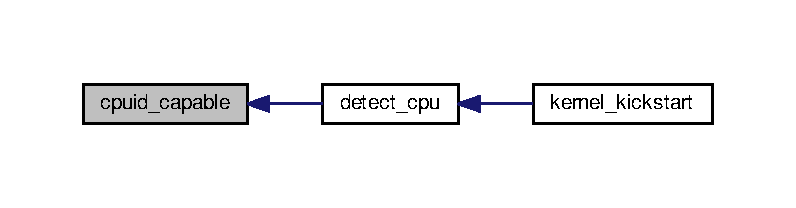
\includegraphics[width=350pt]{cpu_8h_a1a8cb55ce40a2adb1636440c1c20413c_icgraph}
\end{center}
\end{figure}
\mbox{\Hypertarget{cpu_8h_aab96f38dab23a8fc333a33b99d3d7de9}\label{cpu_8h_aab96f38dab23a8fc333a33b99d3d7de9}} 
\index{cpu.\+h@{cpu.\+h}!detect\+\_\+cpu@{detect\+\_\+cpu}}
\index{detect\+\_\+cpu@{detect\+\_\+cpu}!cpu.\+h@{cpu.\+h}}
\subsubsection{\texorpdfstring{detect\+\_\+cpu()}{detect\_cpu()}}
{\footnotesize\ttfamily void detect\+\_\+cpu (\begin{DoxyParamCaption}\item[{void}]{ }\end{DoxyParamCaption})}

Here is the call graph for this function\+:\nopagebreak
\begin{figure}[H]
\begin{center}
\leavevmode
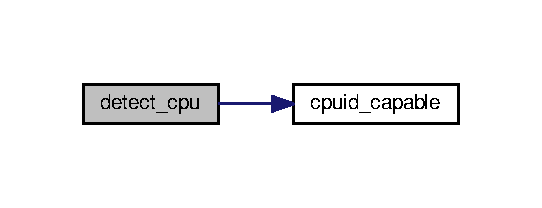
\includegraphics[width=260pt]{cpu_8h_aab96f38dab23a8fc333a33b99d3d7de9_cgraph}
\end{center}
\end{figure}
Here is the caller graph for this function\+:\nopagebreak
\begin{figure}[H]
\begin{center}
\leavevmode
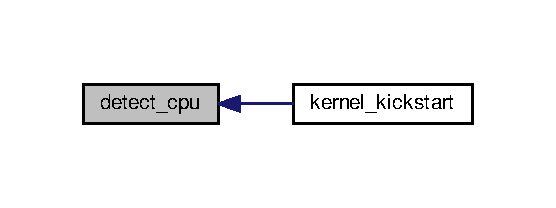
\includegraphics[width=267pt]{cpu_8h_aab96f38dab23a8fc333a33b99d3d7de9_icgraph}
\end{center}
\end{figure}
\mbox{\Hypertarget{cpu_8h_a161ae3250d5ebc057b2784b850564c42}\label{cpu_8h_a161ae3250d5ebc057b2784b850564c42}} 
\index{cpu.\+h@{cpu.\+h}!get\+\_\+cpu\+\_\+info@{get\+\_\+cpu\+\_\+info}}
\index{get\+\_\+cpu\+\_\+info@{get\+\_\+cpu\+\_\+info}!cpu.\+h@{cpu.\+h}}
\subsubsection{\texorpdfstring{get\+\_\+cpu\+\_\+info()}{get\_cpu\_info()}}
{\footnotesize\ttfamily \hyperlink{stddef_8h_a51557cb52bbb9ee9d55aab5b9b16c3d0}{O\+S\+\_\+\+R\+E\+T\+U\+R\+N\+\_\+E} get\+\_\+cpu\+\_\+info (\begin{DoxyParamCaption}\item[{\hyperlink{cpu_8h_a5d0444e34676b8c836666095091ceb88}{cpu\+\_\+info\+\_\+t} $\ast$}]{info }\end{DoxyParamCaption})}

Here is the call graph for this function\+:\nopagebreak
\begin{figure}[H]
\begin{center}
\leavevmode
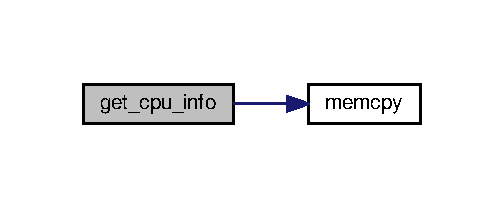
\includegraphics[width=242pt]{cpu_8h_a161ae3250d5ebc057b2784b850564c42_cgraph}
\end{center}
\end{figure}

\hypertarget{cpu__settings_8h}{}\section{/home/alexy/\+Documents/\+Dev/\+R\+T\+L\+K\+I\+M/\+Source/\+Includes/\+Cpu/cpu\+\_\+settings.h File Reference}
\label{cpu__settings_8h}\index{/home/alexy/\+Documents/\+Dev/\+R\+T\+L\+K\+I\+M/\+Source/\+Includes/\+Cpu/cpu\+\_\+settings.\+h@{/home/alexy/\+Documents/\+Dev/\+R\+T\+L\+K\+I\+M/\+Source/\+Includes/\+Cpu/cpu\+\_\+settings.\+h}}
{\ttfamily \#include $<$Lib/stdint.\+h$>$}\newline
Include dependency graph for cpu\+\_\+settings.\+h\+:\nopagebreak
\begin{figure}[H]
\begin{center}
\leavevmode
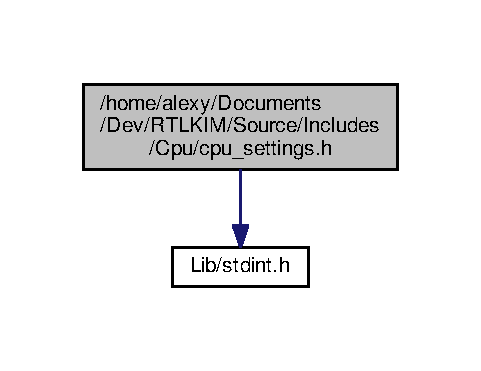
\includegraphics[width=231pt]{cpu__settings_8h__incl}
\end{center}
\end{figure}
This graph shows which files directly or indirectly include this file\+:\nopagebreak
\begin{figure}[H]
\begin{center}
\leavevmode
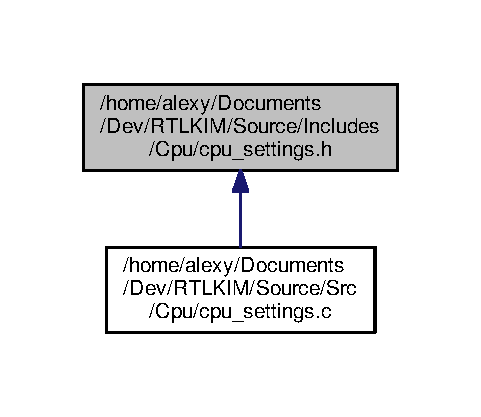
\includegraphics[width=231pt]{cpu__settings_8h__dep__incl}
\end{center}
\end{figure}
\subsection*{Data Structures}
\begin{DoxyCompactItemize}
\item 
struct \hyperlink{structcpu__tss__entry}{cpu\+\_\+tss\+\_\+entry}
\begin{DoxyCompactList}\small\item\em C\+PU T\+SS abstraction structure. This is the representation the kernel has of a intel\textquotesingle{}s T\+SS entry. \end{DoxyCompactList}\end{DoxyCompactItemize}
\subsection*{Macros}
\begin{DoxyCompactItemize}
\item 
\#define \hyperlink{cpu__settings_8h_a297f2b8ecd7aef9861d7b84527ee0c4e}{G\+D\+T\+\_\+\+E\+N\+T\+R\+Y\+\_\+\+C\+O\+U\+NT}~(6 + \hyperlink{config_8h_add08506024a2c5399f9f9f6a797392ef}{M\+A\+X\+\_\+\+C\+P\+U\+\_\+\+C\+O\+U\+NT})
\begin{DoxyCompactList}\small\item\em Number of entries in the kernel\textquotesingle{}s G\+DT. \end{DoxyCompactList}\item 
\#define \hyperlink{cpu__settings_8h_ab0b69b822e9207a5960bc07fc3d36ee4}{K\+E\+R\+N\+E\+L\+\_\+\+CS}~0x08
\begin{DoxyCompactList}\small\item\em Kernel\textquotesingle{}s 32 bits code segment descriptor. \end{DoxyCompactList}\item 
\#define \hyperlink{cpu__settings_8h_a9ab64d7031c0d5cca5b5cca826c4ce63}{K\+E\+R\+N\+E\+L\+\_\+\+DS}~0x10
\begin{DoxyCompactList}\small\item\em Kernel\textquotesingle{}s 32 bits data segment descriptor. \end{DoxyCompactList}\item 
\#define \hyperlink{cpu__settings_8h_a209cb123696486d6801da5e90e443320}{K\+E\+R\+N\+E\+L\+\_\+\+C\+S\+\_\+16}~0x18
\begin{DoxyCompactList}\small\item\em Kernel\textquotesingle{}s 16 bits ode segment descriptor. \end{DoxyCompactList}\item 
\#define \hyperlink{cpu__settings_8h_a717f6ed3322d701e32ccd8d00fde54ac}{K\+E\+R\+N\+E\+L\+\_\+\+D\+S\+\_\+16}~0x20
\begin{DoxyCompactList}\small\item\em Kernel\textquotesingle{}s 16 bits data segment descriptor. \end{DoxyCompactList}\item 
\#define \hyperlink{cpu__settings_8h_a45b4779a5f371471964720229d497c49}{K\+E\+R\+N\+E\+L\+\_\+\+C\+O\+D\+E\+\_\+\+S\+E\+G\+M\+E\+N\+T\+\_\+\+B\+A\+SE}~0x00000000
\begin{DoxyCompactList}\small\item\em Kernel\textquotesingle{}s 32 bits code segment base address. \end{DoxyCompactList}\item 
\#define \hyperlink{cpu__settings_8h_a733a56051fe9d8d045b40167d13a2826}{K\+E\+R\+N\+E\+L\+\_\+\+C\+O\+D\+E\+\_\+\+S\+E\+G\+M\+E\+N\+T\+\_\+\+L\+I\+M\+IT}~0x000\+F\+F\+F\+FF
\begin{DoxyCompactList}\small\item\em Kernel\textquotesingle{}s 32 bits code segment limit address. \end{DoxyCompactList}\item 
\#define \hyperlink{cpu__settings_8h_a2cb21c697525132ee72d44fb295e1d59}{K\+E\+R\+N\+E\+L\+\_\+\+D\+A\+T\+A\+\_\+\+S\+E\+G\+M\+E\+N\+T\+\_\+\+B\+A\+SE}~0x00000000
\begin{DoxyCompactList}\small\item\em Kernel\textquotesingle{}s 32 bits data segment base address. \end{DoxyCompactList}\item 
\#define \hyperlink{cpu__settings_8h_a3419c5adff2115cfb9f51e82f5798c8f}{K\+E\+R\+N\+E\+L\+\_\+\+D\+A\+T\+A\+\_\+\+S\+E\+G\+M\+E\+N\+T\+\_\+\+L\+I\+M\+IT}~0x000\+F\+F\+F\+FF
\begin{DoxyCompactList}\small\item\em Kernel\textquotesingle{}s 32 bits data segment limit address. \end{DoxyCompactList}\item 
\#define \hyperlink{cpu__settings_8h_a0b79c1b48e35895acf4d6e89b55a1aca}{K\+E\+R\+N\+E\+L\+\_\+\+C\+O\+D\+E\+\_\+\+S\+E\+G\+M\+E\+N\+T\+\_\+\+B\+A\+S\+E\+\_\+16}~0x00000000
\begin{DoxyCompactList}\small\item\em Kernel\textquotesingle{}s 16 bits code segment base address. \end{DoxyCompactList}\item 
\#define \hyperlink{cpu__settings_8h_ac6a56aca6a34dc774c4cb01c77d3129c}{K\+E\+R\+N\+E\+L\+\_\+\+C\+O\+D\+E\+\_\+\+S\+E\+G\+M\+E\+N\+T\+\_\+\+L\+I\+M\+I\+T\+\_\+16}~0x000\+F\+F\+F\+FF
\begin{DoxyCompactList}\small\item\em Kernel\textquotesingle{}s 16 bits code segment limit address. \end{DoxyCompactList}\item 
\#define \hyperlink{cpu__settings_8h_a50c283fcfdc7e322496d33d5bcb6465d}{K\+E\+R\+N\+E\+L\+\_\+\+D\+A\+T\+A\+\_\+\+S\+E\+G\+M\+E\+N\+T\+\_\+\+B\+A\+S\+E\+\_\+16}~0x00000000
\begin{DoxyCompactList}\small\item\em Kernel\textquotesingle{}s 16 bits data segment base address. \end{DoxyCompactList}\item 
\#define \hyperlink{cpu__settings_8h_ae2d5346348777e6e576f92b553ffd9d1}{K\+E\+R\+N\+E\+L\+\_\+\+D\+A\+T\+A\+\_\+\+S\+E\+G\+M\+E\+N\+T\+\_\+\+L\+I\+M\+I\+T\+\_\+16}~0x000\+F\+F\+F\+FF
\begin{DoxyCompactList}\small\item\em Kernel\textquotesingle{}s 16 bits data segment limit address. \end{DoxyCompactList}\item 
\#define \hyperlink{cpu__settings_8h_a0c72cb3a158f524fa3efaad5c8d1ce3f}{T\+S\+S\+\_\+\+S\+E\+G\+M\+E\+NT}~0x28
\begin{DoxyCompactList}\small\item\em Kernel\textquotesingle{}s T\+SS segment descriptor. \end{DoxyCompactList}\item 
\#define \hyperlink{cpu__settings_8h_af840df222dbda34ba57520885a74fa01}{G\+D\+T\+\_\+\+F\+L\+A\+G\+\_\+\+G\+R\+A\+N\+U\+L\+A\+R\+I\+T\+Y\+\_\+4K}~0x800000
\begin{DoxyCompactList}\small\item\em G\+DT granularity flag\+: 4K block. \end{DoxyCompactList}\item 
\#define \hyperlink{cpu__settings_8h_a8c36a8afa09883f3b980ef199ebae5aa}{G\+D\+T\+\_\+\+F\+L\+A\+G\+\_\+\+G\+R\+A\+N\+U\+L\+A\+R\+I\+T\+Y\+\_\+\+B\+Y\+TE}~0x000000
\begin{DoxyCompactList}\small\item\em G\+DT granularity flag\+: 1B block. \end{DoxyCompactList}\item 
\#define \hyperlink{cpu__settings_8h_a9c3b234b2effd35a29bf723b9f9fbde0}{G\+D\+T\+\_\+\+F\+L\+A\+G\+\_\+16\+\_\+\+B\+I\+T\+\_\+\+S\+E\+G\+M\+E\+NT}~0x000000
\begin{DoxyCompactList}\small\item\em G\+DT size flag\+: 16b protected mode. \end{DoxyCompactList}\item 
\#define \hyperlink{cpu__settings_8h_a9257f063c14b793f318ccdae39ee8f27}{G\+D\+T\+\_\+\+F\+L\+A\+G\+\_\+32\+\_\+\+B\+I\+T\+\_\+\+S\+E\+G\+M\+E\+NT}~0x400000
\begin{DoxyCompactList}\small\item\em G\+DT size flag\+: 32b protected mode. \end{DoxyCompactList}\item 
\#define \hyperlink{cpu__settings_8h_ad83b0ca80b51513562d604b6623d3034}{G\+D\+T\+\_\+\+F\+L\+A\+G\+\_\+64\+\_\+\+B\+I\+T\+\_\+\+S\+E\+G\+M\+E\+NT}~0x200000
\begin{DoxyCompactList}\small\item\em G\+DT size flag\+: 64b protected mode. \end{DoxyCompactList}\item 
\#define \hyperlink{cpu__settings_8h_a31b7d1d427a6d91d804984e252c85044}{G\+D\+T\+\_\+\+F\+L\+A\+G\+\_\+\+A\+VL}~0x100000
\begin{DoxyCompactList}\small\item\em G\+DT A\+VL flag. \end{DoxyCompactList}\item 
\#define \hyperlink{cpu__settings_8h_a219ae9b0720a036ae9d1ef8e81b67c49}{G\+D\+T\+\_\+\+F\+L\+A\+G\+\_\+\+S\+E\+G\+M\+E\+N\+T\+\_\+\+P\+R\+E\+S\+E\+NT}~0x008000
\begin{DoxyCompactList}\small\item\em G\+DT segment present flag. \end{DoxyCompactList}\item 
\#define \hyperlink{cpu__settings_8h_ab261f28aeb88439bc43657d719306d01}{G\+D\+T\+\_\+\+F\+L\+A\+G\+\_\+\+P\+L0}~0x000000
\begin{DoxyCompactList}\small\item\em G\+DT privilege level flag\+: Ring 0 (kernel). \end{DoxyCompactList}\item 
\#define \hyperlink{cpu__settings_8h_ad14b9fc4e56fbeac8c4c1c3ff498a63a}{G\+D\+T\+\_\+\+F\+L\+A\+G\+\_\+\+P\+L1}~0x002000
\begin{DoxyCompactList}\small\item\em G\+DT privilege level flag\+: Ring 1 (kernel-\/). \end{DoxyCompactList}\item 
\#define \hyperlink{cpu__settings_8h_a2bca87bee848acf0a201d89daa2b48f2}{G\+D\+T\+\_\+\+F\+L\+A\+G\+\_\+\+P\+L2}~0x004000
\begin{DoxyCompactList}\small\item\em G\+DT privilege level flag\+: Ring 2 (kernel--). \end{DoxyCompactList}\item 
\#define \hyperlink{cpu__settings_8h_a47eccc1263d5d986e22553e32bce4d04}{G\+D\+T\+\_\+\+F\+L\+A\+G\+\_\+\+P\+L3}~0x006000
\begin{DoxyCompactList}\small\item\em G\+DT privilege level flag\+: Ring 3 (user). \end{DoxyCompactList}\item 
\#define \hyperlink{cpu__settings_8h_a3f8e70c04de7b1c3a33f1d9133d3b957}{G\+D\+T\+\_\+\+F\+L\+A\+G\+\_\+\+C\+O\+D\+E\+\_\+\+T\+Y\+PE}~0x001000
\begin{DoxyCompactList}\small\item\em G\+DT data type flag\+: code. \end{DoxyCompactList}\item 
\#define \hyperlink{cpu__settings_8h_ad736bb7a475f6ecc8f377a026a2f181c}{G\+D\+T\+\_\+\+F\+L\+A\+G\+\_\+\+D\+A\+T\+A\+\_\+\+T\+Y\+PE}~0x001000
\begin{DoxyCompactList}\small\item\em G\+DT data type flag\+: data. \end{DoxyCompactList}\item 
\#define \hyperlink{cpu__settings_8h_ae9ce26a5aaee07bd87e2221b455da91b}{G\+D\+T\+\_\+\+F\+L\+A\+G\+\_\+\+S\+Y\+S\+T\+E\+M\+\_\+\+T\+Y\+PE}~0x000000
\begin{DoxyCompactList}\small\item\em G\+DT data type flag\+: system. \end{DoxyCompactList}\item 
\#define \hyperlink{cpu__settings_8h_af5da0196f96b610ecd477b62f0ac5305}{G\+D\+T\+\_\+\+F\+L\+A\+G\+\_\+\+T\+SS}~0x09
\begin{DoxyCompactList}\small\item\em G\+DT T\+SS flag. \end{DoxyCompactList}\item 
\#define \hyperlink{cpu__settings_8h_a622798e042fd13d6cd342a4610bd5677}{G\+D\+T\+\_\+\+T\+Y\+P\+E\+\_\+\+E\+X\+E\+C\+U\+T\+A\+B\+LE}~0x8
\begin{DoxyCompactList}\small\item\em G\+DT access byte flag\+: executable. \end{DoxyCompactList}\item 
\#define \hyperlink{cpu__settings_8h_ad5ec8534f87ba806f223ff3558738df5}{G\+D\+T\+\_\+\+T\+Y\+P\+E\+\_\+\+G\+R\+O\+W\+\_\+\+UP}~0x4
\begin{DoxyCompactList}\small\item\em G\+DT access byte flag\+: growth direction up. \end{DoxyCompactList}\item 
\#define \hyperlink{cpu__settings_8h_a61244d895d21e64b65037f5bfb8eec41}{G\+D\+T\+\_\+\+T\+Y\+P\+E\+\_\+\+G\+R\+O\+W\+\_\+\+D\+O\+WN}~0x0
\begin{DoxyCompactList}\small\item\em G\+DT access byte flag\+: growth direction down. \end{DoxyCompactList}\item 
\#define \hyperlink{cpu__settings_8h_a1d5541972939e3db6ab012dfb1e8ca6b}{G\+D\+T\+\_\+\+T\+Y\+P\+E\+\_\+\+C\+O\+N\+F\+O\+R\+M\+I\+NG}~0x4
\begin{DoxyCompactList}\small\item\em G\+DT access byte flag\+: conforming code. \end{DoxyCompactList}\item 
\#define \hyperlink{cpu__settings_8h_a4eb35c96633c8b5efafb96e12bcbe5b2}{G\+D\+T\+\_\+\+T\+Y\+P\+E\+\_\+\+P\+R\+O\+T\+E\+C\+T\+ED}~0x0
\begin{DoxyCompactList}\small\item\em G\+DT access byte flag\+: protected. \end{DoxyCompactList}\item 
\#define \hyperlink{cpu__settings_8h_a798a70f09e14eff9766a987619bb14f5}{G\+D\+T\+\_\+\+T\+Y\+P\+E\+\_\+\+R\+E\+A\+D\+A\+B\+LE}~0x2
\begin{DoxyCompactList}\small\item\em G\+DT access byte flag\+: readable. \end{DoxyCompactList}\item 
\#define \hyperlink{cpu__settings_8h_acaec0cb5d3665b7a965454741f59830e}{G\+D\+T\+\_\+\+T\+Y\+P\+E\+\_\+\+W\+R\+I\+T\+A\+B\+LE}~0x2
\begin{DoxyCompactList}\small\item\em G\+DT access byte flag\+: writable. \end{DoxyCompactList}\item 
\#define \hyperlink{cpu__settings_8h_a969141801108555f5cfdbf86c8525da1}{G\+D\+T\+\_\+\+T\+Y\+P\+E\+\_\+\+A\+C\+C\+E\+S\+S\+ED}~0x1
\begin{DoxyCompactList}\small\item\em G\+DT access byte flag\+: accessed byte. \end{DoxyCompactList}\item 
\#define \hyperlink{cpu__settings_8h_ac5ba6506506314600fc35d49780e0072}{I\+D\+T\+\_\+\+E\+N\+T\+R\+Y\+\_\+\+C\+O\+U\+NT}~256
\begin{DoxyCompactList}\small\item\em Number of entries in the kernel\textquotesingle{}s I\+DT. \end{DoxyCompactList}\item 
\#define \hyperlink{cpu__settings_8h_a9a6527e55b5e135419c71b7283f5a5b2}{I\+D\+T\+\_\+\+F\+L\+A\+G\+\_\+\+S\+T\+O\+R\+A\+G\+E\+\_\+\+S\+EG}~0x10
\begin{DoxyCompactList}\small\item\em I\+DT flag\+: storage segment. \end{DoxyCompactList}\item 
\#define \hyperlink{cpu__settings_8h_ad9fe2663969501bcffb2ce7f50de4321}{I\+D\+T\+\_\+\+F\+L\+A\+G\+\_\+\+P\+L0}~0x00
\begin{DoxyCompactList}\small\item\em I\+DT flag\+: privilege level, ring 0. \end{DoxyCompactList}\item 
\#define \hyperlink{cpu__settings_8h_aa324eb394bc82d8df6c28ee306b87e5a}{I\+D\+T\+\_\+\+F\+L\+A\+G\+\_\+\+P\+L1}~0x20
\begin{DoxyCompactList}\small\item\em I\+DT flag\+: privilege level, ring 1. \end{DoxyCompactList}\item 
\#define \hyperlink{cpu__settings_8h_a2a33a16204bac35f6d563318b3239777}{I\+D\+T\+\_\+\+F\+L\+A\+G\+\_\+\+P\+L2}~0x40
\begin{DoxyCompactList}\small\item\em I\+DT flag\+: privilege level, ring 2. \end{DoxyCompactList}\item 
\#define \hyperlink{cpu__settings_8h_a2a29a1265ef69b55bfa5a5e3e664bf91}{I\+D\+T\+\_\+\+F\+L\+A\+G\+\_\+\+P\+L3}~0x60
\begin{DoxyCompactList}\small\item\em I\+DT flag\+: privilege level, ring 3. \end{DoxyCompactList}\item 
\#define \hyperlink{cpu__settings_8h_a655be59845ed69ebd5b95e3ec05a0671}{I\+D\+T\+\_\+\+F\+L\+A\+G\+\_\+\+P\+R\+E\+S\+E\+NT}~0x80
\begin{DoxyCompactList}\small\item\em I\+DT flag\+: interrupt present. \end{DoxyCompactList}\item 
\#define \hyperlink{cpu__settings_8h_a98743f57f10f81b4d6ebaa17f5e8c503}{I\+D\+T\+\_\+\+T\+Y\+P\+E\+\_\+\+T\+A\+S\+K\+\_\+\+G\+A\+TE}~0x05
\begin{DoxyCompactList}\small\item\em I\+DT flag\+: interrupt type task gate. \end{DoxyCompactList}\item 
\#define \hyperlink{cpu__settings_8h_a02d9fee9afa3f2e0c88f95ef47cb9141}{I\+D\+T\+\_\+\+T\+Y\+P\+E\+\_\+\+I\+N\+T\+\_\+\+G\+A\+TE}~0x0E
\begin{DoxyCompactList}\small\item\em I\+DT flag\+: interrupt type interrupt gate. \end{DoxyCompactList}\item 
\#define \hyperlink{cpu__settings_8h_a1021029b5a224a966cb356460a4aba48}{I\+D\+T\+\_\+\+T\+Y\+P\+E\+\_\+\+T\+R\+A\+P\+\_\+\+G\+A\+TE}~0x0F
\begin{DoxyCompactList}\small\item\em I\+DT flag\+: interrupt type trap gate. \end{DoxyCompactList}\end{DoxyCompactItemize}
\subsection*{Typedefs}
\begin{DoxyCompactItemize}
\item 
typedef struct \hyperlink{structcpu__tss__entry}{cpu\+\_\+tss\+\_\+entry} \hyperlink{cpu__settings_8h_aafb7832b0df405ea5f84be132221805b}{cpu\+\_\+tss\+\_\+entry\+\_\+t}
\begin{DoxyCompactList}\small\item\em Defines the cpu\+\_\+tss\+\_\+entry\+\_\+t type as a shortcut for struct \hyperlink{structcpu__tss__entry}{cpu\+\_\+tss\+\_\+entry}. \end{DoxyCompactList}\end{DoxyCompactItemize}
\subsection*{Functions}
\begin{DoxyCompactItemize}
\item 
void \hyperlink{cpu__settings_8h_a43b34e010346446043e35b7836be7aaa}{interrupt\+\_\+handler\+\_\+0} (void)
\begin{DoxyCompactList}\small\item\em Assembly interrupt handler for line 0. Saves the context and calls the generic interrupt handler. \end{DoxyCompactList}\item 
void \hyperlink{cpu__settings_8h_aaa0d1c3fa5553012fa513c3323e1b887}{interrupt\+\_\+handler\+\_\+1} (void)
\begin{DoxyCompactList}\small\item\em Assembly interrupt handler for line 1. Saves the context and calls the generic interrupt handler. \end{DoxyCompactList}\item 
void \hyperlink{cpu__settings_8h_ab594ae9e5df33e8ce977ecc38aaa2687}{interrupt\+\_\+handler\+\_\+2} (void)
\begin{DoxyCompactList}\small\item\em Assembly interrupt handler for line 2. Saves the context and calls the generic interrupt handler. \end{DoxyCompactList}\item 
void \hyperlink{cpu__settings_8h_a7fc1aecf219b20a4dd71135e50ff6d81}{interrupt\+\_\+handler\+\_\+3} (void)
\begin{DoxyCompactList}\small\item\em Assembly interrupt handler for line 3. Saves the context and calls the generic interrupt handler. \end{DoxyCompactList}\item 
void \hyperlink{cpu__settings_8h_ae92a794cb2ac32a5ca5259173ab6eb5d}{interrupt\+\_\+handler\+\_\+4} (void)
\begin{DoxyCompactList}\small\item\em Assembly interrupt handler for line 4. Saves the context and calls the generic interrupt handler. \end{DoxyCompactList}\item 
void \hyperlink{cpu__settings_8h_a22e84a29454fadb3699bf97806917c1b}{interrupt\+\_\+handler\+\_\+5} (void)
\begin{DoxyCompactList}\small\item\em Assembly interrupt handler for line 5. Saves the context and calls the generic interrupt handler. \end{DoxyCompactList}\item 
void \hyperlink{cpu__settings_8h_a61843bbac596cf22db3953b216a1dfa4}{interrupt\+\_\+handler\+\_\+6} (void)
\begin{DoxyCompactList}\small\item\em Assembly interrupt handler for line 6. Saves the context and calls the generic interrupt handler. \end{DoxyCompactList}\item 
void \hyperlink{cpu__settings_8h_a83d43513ad0f83f21bda3fca881b9af9}{interrupt\+\_\+handler\+\_\+7} (void)
\begin{DoxyCompactList}\small\item\em Assembly interrupt handler for line 7. Saves the context and calls the generic interrupt handler. \end{DoxyCompactList}\item 
void \hyperlink{cpu__settings_8h_a7ed9dffc66f69905e6dd94d84ebdbd30}{interrupt\+\_\+handler\+\_\+8} (void)
\begin{DoxyCompactList}\small\item\em Assembly interrupt handler for line 8. Saves the context and calls the generic interrupt handler. \end{DoxyCompactList}\item 
void \hyperlink{cpu__settings_8h_ab0d38da581a58307c9dd81cea4de70de}{interrupt\+\_\+handler\+\_\+9} (void)
\begin{DoxyCompactList}\small\item\em Assembly interrupt handler for line 9. Saves the context and calls the generic interrupt handler. \end{DoxyCompactList}\item 
void \hyperlink{cpu__settings_8h_ab8168b58edea58df6bb402936705e67f}{interrupt\+\_\+handler\+\_\+10} (void)
\begin{DoxyCompactList}\small\item\em Assembly interrupt handler for line 10. Saves the context and calls the generic interrupt handler. \end{DoxyCompactList}\item 
void \hyperlink{cpu__settings_8h_a4ee7baba233e4aff1c4a96dad6e68cd9}{interrupt\+\_\+handler\+\_\+11} (void)
\begin{DoxyCompactList}\small\item\em Assembly interrupt handler for line 11. Saves the context and calls the generic interrupt handler. \end{DoxyCompactList}\item 
void \hyperlink{cpu__settings_8h_afe2632e7657960a7548d574432d5baee}{interrupt\+\_\+handler\+\_\+12} (void)
\begin{DoxyCompactList}\small\item\em Assembly interrupt handler for line 12. Saves the context and calls the generic interrupt handler. \end{DoxyCompactList}\item 
void \hyperlink{cpu__settings_8h_a7615969931a2800e19627f6c97090c31}{interrupt\+\_\+handler\+\_\+13} (void)
\begin{DoxyCompactList}\small\item\em Assembly interrupt handler for line 13. Saves the context and calls the generic interrupt handler. \end{DoxyCompactList}\item 
void \hyperlink{cpu__settings_8h_a118ac4236854fbe879353c12817d5582}{interrupt\+\_\+handler\+\_\+14} (void)
\begin{DoxyCompactList}\small\item\em Assembly interrupt handler for line 14. Saves the context and calls the generic interrupt handler. \end{DoxyCompactList}\item 
void \hyperlink{cpu__settings_8h_adf7c6ec9e458e494a7bbe5454157a451}{interrupt\+\_\+handler\+\_\+15} (void)
\begin{DoxyCompactList}\small\item\em Assembly interrupt handler for line 15. Saves the context and calls the generic interrupt handler. \end{DoxyCompactList}\item 
void \hyperlink{cpu__settings_8h_a546360384b8b6f9ee11fa3f04db48728}{interrupt\+\_\+handler\+\_\+16} (void)
\begin{DoxyCompactList}\small\item\em Assembly interrupt handler for line 16. Saves the context and calls the generic interrupt handler. \end{DoxyCompactList}\item 
void \hyperlink{cpu__settings_8h_a91a9d111654bdddfbebdb8678588770a}{interrupt\+\_\+handler\+\_\+17} (void)
\begin{DoxyCompactList}\small\item\em Assembly interrupt handler for line 17. Saves the context and calls the generic interrupt handler. \end{DoxyCompactList}\item 
void \hyperlink{cpu__settings_8h_afb3b70c635c323f214bb3e9cf72a5d4f}{interrupt\+\_\+handler\+\_\+18} (void)
\begin{DoxyCompactList}\small\item\em Assembly interrupt handler for line 18. Saves the context and calls the generic interrupt handler. \end{DoxyCompactList}\item 
void \hyperlink{cpu__settings_8h_ad15538d51b0c4301e5b8cbe83c823df8}{interrupt\+\_\+handler\+\_\+19} (void)
\begin{DoxyCompactList}\small\item\em Assembly interrupt handler for line 19. Saves the context and calls the generic interrupt handler. \end{DoxyCompactList}\item 
void \hyperlink{cpu__settings_8h_ab69188cf232400c32abe9a387fa5a729}{interrupt\+\_\+handler\+\_\+20} (void)
\begin{DoxyCompactList}\small\item\em Assembly interrupt handler for line 20. Saves the context and calls the generic interrupt handler. \end{DoxyCompactList}\item 
void \hyperlink{cpu__settings_8h_a160985e1f446db0de039ba3cf206a6f1}{interrupt\+\_\+handler\+\_\+21} (void)
\begin{DoxyCompactList}\small\item\em Assembly interrupt handler for line 21. Saves the context and calls the generic interrupt handler. \end{DoxyCompactList}\item 
void \hyperlink{cpu__settings_8h_a8cc949332175f392dc94547044e5719d}{interrupt\+\_\+handler\+\_\+22} (void)
\begin{DoxyCompactList}\small\item\em Assembly interrupt handler for line 22. Saves the context and calls the generic interrupt handler. \end{DoxyCompactList}\item 
void \hyperlink{cpu__settings_8h_a3942237004f6a315de322d69fa139481}{interrupt\+\_\+handler\+\_\+23} (void)
\begin{DoxyCompactList}\small\item\em Assembly interrupt handler for line 23. Saves the context and calls the generic interrupt handler. \end{DoxyCompactList}\item 
void \hyperlink{cpu__settings_8h_a591b6b2716e4bbc9bb79dddb070f4cdb}{interrupt\+\_\+handler\+\_\+24} (void)
\begin{DoxyCompactList}\small\item\em Assembly interrupt handler for line 24. Saves the context and calls the generic interrupt handler. \end{DoxyCompactList}\item 
void \hyperlink{cpu__settings_8h_a3f30bd1727ea1c5d455a552cf234db7d}{interrupt\+\_\+handler\+\_\+25} (void)
\begin{DoxyCompactList}\small\item\em Assembly interrupt handler for line 25. Saves the context and calls the generic interrupt handler. \end{DoxyCompactList}\item 
void \hyperlink{cpu__settings_8h_a77d335b9042655a02afab23acd97b6a4}{interrupt\+\_\+handler\+\_\+26} (void)
\begin{DoxyCompactList}\small\item\em Assembly interrupt handler for line 26. Saves the context and calls the generic interrupt handler. \end{DoxyCompactList}\item 
void \hyperlink{cpu__settings_8h_afa055d5a92fb22b6a5e95735a230e349}{interrupt\+\_\+handler\+\_\+27} (void)
\begin{DoxyCompactList}\small\item\em Assembly interrupt handler for line 27. Saves the context and calls the generic interrupt handler. \end{DoxyCompactList}\item 
void \hyperlink{cpu__settings_8h_a712d037de97f7481f241f7cd4b128a0a}{interrupt\+\_\+handler\+\_\+28} (void)
\begin{DoxyCompactList}\small\item\em Assembly interrupt handler for line 28. Saves the context and calls the generic interrupt handler. \end{DoxyCompactList}\item 
void \hyperlink{cpu__settings_8h_afd1ca083a8e1d4faccc928777ad69726}{interrupt\+\_\+handler\+\_\+29} (void)
\begin{DoxyCompactList}\small\item\em Assembly interrupt handler for line 29. Saves the context and calls the generic interrupt handler. \end{DoxyCompactList}\item 
void \hyperlink{cpu__settings_8h_a58e78cce854c364297ba843b0ee65f05}{interrupt\+\_\+handler\+\_\+30} (void)
\begin{DoxyCompactList}\small\item\em Assembly interrupt handler for line 30. Saves the context and calls the generic interrupt handler. \end{DoxyCompactList}\item 
void \hyperlink{cpu__settings_8h_abc8f9ed4111dc7febfd33b2263b2ebf3}{interrupt\+\_\+handler\+\_\+31} (void)
\begin{DoxyCompactList}\small\item\em Assembly interrupt handler for line 31. Saves the context and calls the generic interrupt handler. \end{DoxyCompactList}\item 
void \hyperlink{cpu__settings_8h_a8c34fb2ca26413d93e9bcfb288d858f7}{interrupt\+\_\+handler\+\_\+32} (void)
\begin{DoxyCompactList}\small\item\em Assembly interrupt handler for line 32. Saves the context and calls the generic interrupt handler. \end{DoxyCompactList}\item 
void \hyperlink{cpu__settings_8h_a3d0ceb38061ba22cef80fc1be0d5ad42}{interrupt\+\_\+handler\+\_\+33} (void)
\begin{DoxyCompactList}\small\item\em Assembly interrupt handler for line 33. Saves the context and calls the generic interrupt handler. \end{DoxyCompactList}\item 
void \hyperlink{cpu__settings_8h_a0353aaf01938e4fea3c7665f5ee0358f}{interrupt\+\_\+handler\+\_\+34} (void)
\begin{DoxyCompactList}\small\item\em Assembly interrupt handler for line 34. Saves the context and calls the generic interrupt handler. \end{DoxyCompactList}\item 
void \hyperlink{cpu__settings_8h_a0758c9e7eaf1700afb5e98c63c3ca486}{interrupt\+\_\+handler\+\_\+35} (void)
\begin{DoxyCompactList}\small\item\em Assembly interrupt handler for line 35. Saves the context and calls the generic interrupt handler. \end{DoxyCompactList}\item 
void \hyperlink{cpu__settings_8h_ab5970ac4efac6943036ebda4e061099c}{interrupt\+\_\+handler\+\_\+36} (void)
\begin{DoxyCompactList}\small\item\em Assembly interrupt handler for line 36. Saves the context and calls the generic interrupt handler. \end{DoxyCompactList}\item 
void \hyperlink{cpu__settings_8h_a8a191c69a85706384bba5af54ec4db65}{interrupt\+\_\+handler\+\_\+37} (void)
\begin{DoxyCompactList}\small\item\em Assembly interrupt handler for line 37. Saves the context and calls the generic interrupt handler. \end{DoxyCompactList}\item 
void \hyperlink{cpu__settings_8h_a21b652e001fcbf3ea8adef0c41e9f1f6}{interrupt\+\_\+handler\+\_\+38} (void)
\begin{DoxyCompactList}\small\item\em Assembly interrupt handler for line 38. Saves the context and calls the generic interrupt handler. \end{DoxyCompactList}\item 
void \hyperlink{cpu__settings_8h_ab4de5e0231f4b30791702f6a28364f22}{interrupt\+\_\+handler\+\_\+39} (void)
\begin{DoxyCompactList}\small\item\em Assembly interrupt handler for line 39. Saves the context and calls the generic interrupt handler. \end{DoxyCompactList}\item 
void \hyperlink{cpu__settings_8h_a1b680de1e0155773ef5804c841adcd20}{interrupt\+\_\+handler\+\_\+40} (void)
\begin{DoxyCompactList}\small\item\em Assembly interrupt handler for line 40. Saves the context and calls the generic interrupt handler. \end{DoxyCompactList}\item 
void \hyperlink{cpu__settings_8h_aaa16ecbddd21174ebfb2e3c7275dce47}{interrupt\+\_\+handler\+\_\+41} (void)
\begin{DoxyCompactList}\small\item\em Assembly interrupt handler for line 41. Saves the context and calls the generic interrupt handler. \end{DoxyCompactList}\item 
void \hyperlink{cpu__settings_8h_a634af1029b7c20e032a9a132f85df1b3}{interrupt\+\_\+handler\+\_\+42} (void)
\begin{DoxyCompactList}\small\item\em Assembly interrupt handler for line 42. Saves the context and calls the generic interrupt handler. \end{DoxyCompactList}\item 
void \hyperlink{cpu__settings_8h_a887539f52d303d757d89a541d951b7b7}{interrupt\+\_\+handler\+\_\+43} (void)
\begin{DoxyCompactList}\small\item\em Assembly interrupt handler for line 43. Saves the context and calls the generic interrupt handler. \end{DoxyCompactList}\item 
void \hyperlink{cpu__settings_8h_ae82c89ac0416233f89cedeafc69ef58d}{interrupt\+\_\+handler\+\_\+44} (void)
\begin{DoxyCompactList}\small\item\em Assembly interrupt handler for line 44. Saves the context and calls the generic interrupt handler. \end{DoxyCompactList}\item 
void \hyperlink{cpu__settings_8h_a10b0ddffea254b075edf66b2cfa847da}{interrupt\+\_\+handler\+\_\+45} (void)
\begin{DoxyCompactList}\small\item\em Assembly interrupt handler for line 45. Saves the context and calls the generic interrupt handler. \end{DoxyCompactList}\item 
void \hyperlink{cpu__settings_8h_a617a01f7e8a3ab6c79a7125798c7cfb9}{interrupt\+\_\+handler\+\_\+46} (void)
\begin{DoxyCompactList}\small\item\em Assembly interrupt handler for line 46. Saves the context and calls the generic interrupt handler. \end{DoxyCompactList}\item 
void \hyperlink{cpu__settings_8h_a8c80d599088667a39f1cbb8dc9fd6fee}{interrupt\+\_\+handler\+\_\+47} (void)
\begin{DoxyCompactList}\small\item\em Assembly interrupt handler for line 47. Saves the context and calls the generic interrupt handler. \end{DoxyCompactList}\item 
void \hyperlink{cpu__settings_8h_aa30a38394a1c35b05e2ae7041d153c23}{interrupt\+\_\+handler\+\_\+48} (void)
\begin{DoxyCompactList}\small\item\em Assembly interrupt handler for line 48. Saves the context and calls the generic interrupt handler. \end{DoxyCompactList}\item 
void \hyperlink{cpu__settings_8h_a9d40e7527e44e5ed7ea8dbe7f80b2dc7}{interrupt\+\_\+handler\+\_\+49} (void)
\begin{DoxyCompactList}\small\item\em Assembly interrupt handler for line 49. Saves the context and calls the generic interrupt handler. \end{DoxyCompactList}\item 
void \hyperlink{cpu__settings_8h_a0207e50ba4fcd827440d29ef22f5d3b5}{interrupt\+\_\+handler\+\_\+50} (void)
\begin{DoxyCompactList}\small\item\em Assembly interrupt handler for line 50. Saves the context and calls the generic interrupt handler. \end{DoxyCompactList}\item 
void \hyperlink{cpu__settings_8h_ac13f17f69824223dd03af18c193b28e7}{interrupt\+\_\+handler\+\_\+51} (void)
\begin{DoxyCompactList}\small\item\em Assembly interrupt handler for line 51. Saves the context and calls the generic interrupt handler. \end{DoxyCompactList}\item 
void \hyperlink{cpu__settings_8h_a7e0c89be7f1be3d3506303db9390c451}{interrupt\+\_\+handler\+\_\+52} (void)
\begin{DoxyCompactList}\small\item\em Assembly interrupt handler for line 52. Saves the context and calls the generic interrupt handler. \end{DoxyCompactList}\item 
void \hyperlink{cpu__settings_8h_a38bc9ca51a51c8c67f8892932d832c1f}{interrupt\+\_\+handler\+\_\+53} (void)
\begin{DoxyCompactList}\small\item\em Assembly interrupt handler for line 53. Saves the context and calls the generic interrupt handler. \end{DoxyCompactList}\item 
void \hyperlink{cpu__settings_8h_a99c50e4c9604faf72747a79669f3dfd9}{interrupt\+\_\+handler\+\_\+54} (void)
\begin{DoxyCompactList}\small\item\em Assembly interrupt handler for line 54. Saves the context and calls the generic interrupt handler. \end{DoxyCompactList}\item 
void \hyperlink{cpu__settings_8h_a28c87ead6a169e35862443802a2855a8}{interrupt\+\_\+handler\+\_\+55} (void)
\begin{DoxyCompactList}\small\item\em Assembly interrupt handler for line 55. Saves the context and calls the generic interrupt handler. \end{DoxyCompactList}\item 
void \hyperlink{cpu__settings_8h_afda559c1a90dc12c873028c0a2417eb7}{interrupt\+\_\+handler\+\_\+56} (void)
\begin{DoxyCompactList}\small\item\em Assembly interrupt handler for line 56. Saves the context and calls the generic interrupt handler. \end{DoxyCompactList}\item 
void \hyperlink{cpu__settings_8h_a70ed87ebdb1418431386809de935fcfb}{interrupt\+\_\+handler\+\_\+57} (void)
\begin{DoxyCompactList}\small\item\em Assembly interrupt handler for line 57. Saves the context and calls the generic interrupt handler. \end{DoxyCompactList}\item 
void \hyperlink{cpu__settings_8h_a1326304073b4cd37ebe27254b67dfd42}{interrupt\+\_\+handler\+\_\+58} (void)
\begin{DoxyCompactList}\small\item\em Assembly interrupt handler for line 58. Saves the context and calls the generic interrupt handler. \end{DoxyCompactList}\item 
void \hyperlink{cpu__settings_8h_ac1992b56ac22afe2eb07a142abde9872}{interrupt\+\_\+handler\+\_\+59} (void)
\begin{DoxyCompactList}\small\item\em Assembly interrupt handler for line 59. Saves the context and calls the generic interrupt handler. \end{DoxyCompactList}\item 
void \hyperlink{cpu__settings_8h_a890210fa78243d642cc105feda82ba69}{interrupt\+\_\+handler\+\_\+60} (void)
\begin{DoxyCompactList}\small\item\em Assembly interrupt handler for line 60. Saves the context and calls the generic interrupt handler. \end{DoxyCompactList}\item 
void \hyperlink{cpu__settings_8h_a13397e5bac48585efdeb9e496eaf4c80}{interrupt\+\_\+handler\+\_\+61} (void)
\begin{DoxyCompactList}\small\item\em Assembly interrupt handler for line 61. Saves the context and calls the generic interrupt handler. \end{DoxyCompactList}\item 
void \hyperlink{cpu__settings_8h_a1aab93ec8cf396028d7f7a124cb2919e}{interrupt\+\_\+handler\+\_\+62} (void)
\begin{DoxyCompactList}\small\item\em Assembly interrupt handler for line 62. Saves the context and calls the generic interrupt handler. \end{DoxyCompactList}\item 
void \hyperlink{cpu__settings_8h_a798dc204538b6398095a9102f42fda81}{interrupt\+\_\+handler\+\_\+63} (void)
\begin{DoxyCompactList}\small\item\em Assembly interrupt handler for line 63. Saves the context and calls the generic interrupt handler. \end{DoxyCompactList}\item 
void \hyperlink{cpu__settings_8h_ae41f97308aae96455afd6a7462660d17}{interrupt\+\_\+handler\+\_\+64} (void)
\begin{DoxyCompactList}\small\item\em Assembly interrupt handler for line 64. Saves the context and calls the generic interrupt handler. \end{DoxyCompactList}\item 
void \hyperlink{cpu__settings_8h_a885f07fd3961b44108b8b2cdc8ae2bf5}{interrupt\+\_\+handler\+\_\+65} (void)
\begin{DoxyCompactList}\small\item\em Assembly interrupt handler for line 65. Saves the context and calls the generic interrupt handler. \end{DoxyCompactList}\item 
void \hyperlink{cpu__settings_8h_a538845f3792c177c694049c0b54129f1}{interrupt\+\_\+handler\+\_\+66} (void)
\begin{DoxyCompactList}\small\item\em Assembly interrupt handler for line 66. Saves the context and calls the generic interrupt handler. \end{DoxyCompactList}\item 
void \hyperlink{cpu__settings_8h_a4238d54456d67401ef6d39c3b8d85b41}{interrupt\+\_\+handler\+\_\+67} (void)
\begin{DoxyCompactList}\small\item\em Assembly interrupt handler for line 67. Saves the context and calls the generic interrupt handler. \end{DoxyCompactList}\item 
void \hyperlink{cpu__settings_8h_a53084fa59eff21d88980d1f9b26e22e3}{interrupt\+\_\+handler\+\_\+68} (void)
\begin{DoxyCompactList}\small\item\em Assembly interrupt handler for line 68. Saves the context and calls the generic interrupt handler. \end{DoxyCompactList}\item 
void \hyperlink{cpu__settings_8h_a5af5622b73f6c2fd90ea7d01d66aeaac}{interrupt\+\_\+handler\+\_\+69} (void)
\begin{DoxyCompactList}\small\item\em Assembly interrupt handler for line 69. Saves the context and calls the generic interrupt handler. \end{DoxyCompactList}\item 
void \hyperlink{cpu__settings_8h_a7d9a0027bb610328de0d5f0a93ec55e8}{interrupt\+\_\+handler\+\_\+70} (void)
\begin{DoxyCompactList}\small\item\em Assembly interrupt handler for line 70. Saves the context and calls the generic interrupt handler. \end{DoxyCompactList}\item 
void \hyperlink{cpu__settings_8h_a402efad0670a1ffc4c021432e46817dd}{interrupt\+\_\+handler\+\_\+71} (void)
\begin{DoxyCompactList}\small\item\em Assembly interrupt handler for line 71. Saves the context and calls the generic interrupt handler. \end{DoxyCompactList}\item 
void \hyperlink{cpu__settings_8h_af18438b45cafdf14c667ac870946dd0b}{interrupt\+\_\+handler\+\_\+72} (void)
\begin{DoxyCompactList}\small\item\em Assembly interrupt handler for line 72. Saves the context and calls the generic interrupt handler. \end{DoxyCompactList}\item 
void \hyperlink{cpu__settings_8h_a141f7e9eb0f23e7063c726ee5c7c626f}{interrupt\+\_\+handler\+\_\+73} (void)
\begin{DoxyCompactList}\small\item\em Assembly interrupt handler for line 73. Saves the context and calls the generic interrupt handler. \end{DoxyCompactList}\item 
void \hyperlink{cpu__settings_8h_a1d554c2278e3e578f8e6a58e9fc53be8}{interrupt\+\_\+handler\+\_\+74} (void)
\begin{DoxyCompactList}\small\item\em Assembly interrupt handler for line 74. Saves the context and calls the generic interrupt handler. \end{DoxyCompactList}\item 
void \hyperlink{cpu__settings_8h_aa8a0564751d18f6642e3e45f60f512c9}{interrupt\+\_\+handler\+\_\+75} (void)
\begin{DoxyCompactList}\small\item\em Assembly interrupt handler for line 75. Saves the context and calls the generic interrupt handler. \end{DoxyCompactList}\item 
void \hyperlink{cpu__settings_8h_a6b7362bc00c89f0ce788c3c6c7d50d3d}{interrupt\+\_\+handler\+\_\+76} (void)
\begin{DoxyCompactList}\small\item\em Assembly interrupt handler for line 76. Saves the context and calls the generic interrupt handler. \end{DoxyCompactList}\item 
void \hyperlink{cpu__settings_8h_afbd866b040d8d71e6c89a2475840b969}{interrupt\+\_\+handler\+\_\+77} (void)
\begin{DoxyCompactList}\small\item\em Assembly interrupt handler for line 77. Saves the context and calls the generic interrupt handler. \end{DoxyCompactList}\item 
void \hyperlink{cpu__settings_8h_a74f4f7a5fcee27dd1cebc061fe666216}{interrupt\+\_\+handler\+\_\+78} (void)
\begin{DoxyCompactList}\small\item\em Assembly interrupt handler for line 78. Saves the context and calls the generic interrupt handler. \end{DoxyCompactList}\item 
void \hyperlink{cpu__settings_8h_a49e83bb69076b5c561bc082f703cc193}{interrupt\+\_\+handler\+\_\+79} (void)
\begin{DoxyCompactList}\small\item\em Assembly interrupt handler for line 79. Saves the context and calls the generic interrupt handler. \end{DoxyCompactList}\item 
void \hyperlink{cpu__settings_8h_adcf5896b9b05c8c38245048b498ac59b}{interrupt\+\_\+handler\+\_\+80} (void)
\begin{DoxyCompactList}\small\item\em Assembly interrupt handler for line 80. Saves the context and calls the generic interrupt handler. \end{DoxyCompactList}\item 
void \hyperlink{cpu__settings_8h_a3eb0a2fea5857024adeeb9a683960ac8}{interrupt\+\_\+handler\+\_\+81} (void)
\begin{DoxyCompactList}\small\item\em Assembly interrupt handler for line 81. Saves the context and calls the generic interrupt handler. \end{DoxyCompactList}\item 
void \hyperlink{cpu__settings_8h_a32326dd7fdca122dbe6ee50189563f6a}{interrupt\+\_\+handler\+\_\+82} (void)
\begin{DoxyCompactList}\small\item\em Assembly interrupt handler for line 82. Saves the context and calls the generic interrupt handler. \end{DoxyCompactList}\item 
void \hyperlink{cpu__settings_8h_afce2b6141809aa4fcc58172ddafd9086}{interrupt\+\_\+handler\+\_\+83} (void)
\begin{DoxyCompactList}\small\item\em Assembly interrupt handler for line 83. Saves the context and calls the generic interrupt handler. \end{DoxyCompactList}\item 
void \hyperlink{cpu__settings_8h_a9c95276039af36cbef353bbfd40413b5}{interrupt\+\_\+handler\+\_\+84} (void)
\begin{DoxyCompactList}\small\item\em Assembly interrupt handler for line 84. Saves the context and calls the generic interrupt handler. \end{DoxyCompactList}\item 
void \hyperlink{cpu__settings_8h_aff46870c650c9863bb1c4eb266dbbc7a}{interrupt\+\_\+handler\+\_\+85} (void)
\begin{DoxyCompactList}\small\item\em Assembly interrupt handler for line 85. Saves the context and calls the generic interrupt handler. \end{DoxyCompactList}\item 
void \hyperlink{cpu__settings_8h_a56fd87617557a6a8bfb0f97921b2f41d}{interrupt\+\_\+handler\+\_\+86} (void)
\begin{DoxyCompactList}\small\item\em Assembly interrupt handler for line 86. Saves the context and calls the generic interrupt handler. \end{DoxyCompactList}\item 
void \hyperlink{cpu__settings_8h_ab626af2edec92ef4cc7c772e0ec08bc0}{interrupt\+\_\+handler\+\_\+87} (void)
\begin{DoxyCompactList}\small\item\em Assembly interrupt handler for line 87. Saves the context and calls the generic interrupt handler. \end{DoxyCompactList}\item 
void \hyperlink{cpu__settings_8h_a33bcf7336bce8686bd0918676b2b946f}{interrupt\+\_\+handler\+\_\+88} (void)
\begin{DoxyCompactList}\small\item\em Assembly interrupt handler for line 88. Saves the context and calls the generic interrupt handler. \end{DoxyCompactList}\item 
void \hyperlink{cpu__settings_8h_a6b992a177073c5da8a89444a1716cdc7}{interrupt\+\_\+handler\+\_\+89} (void)
\begin{DoxyCompactList}\small\item\em Assembly interrupt handler for line 89. Saves the context and calls the generic interrupt handler. \end{DoxyCompactList}\item 
void \hyperlink{cpu__settings_8h_af63c70691bbfc03102bb41191960ade1}{interrupt\+\_\+handler\+\_\+90} (void)
\begin{DoxyCompactList}\small\item\em Assembly interrupt handler for line 90. Saves the context and calls the generic interrupt handler. \end{DoxyCompactList}\item 
void \hyperlink{cpu__settings_8h_acba8dd6af4bbe024db28afa3cabe1836}{interrupt\+\_\+handler\+\_\+91} (void)
\begin{DoxyCompactList}\small\item\em Assembly interrupt handler for line 91. Saves the context and calls the generic interrupt handler. \end{DoxyCompactList}\item 
void \hyperlink{cpu__settings_8h_af59b08ea13d0ea4702efcba877429db5}{interrupt\+\_\+handler\+\_\+92} (void)
\begin{DoxyCompactList}\small\item\em Assembly interrupt handler for line 92. Saves the context and calls the generic interrupt handler. \end{DoxyCompactList}\item 
void \hyperlink{cpu__settings_8h_ae548bad74c08a961c4694ae5dacdc5b7}{interrupt\+\_\+handler\+\_\+93} (void)
\begin{DoxyCompactList}\small\item\em Assembly interrupt handler for line 93. Saves the context and calls the generic interrupt handler. \end{DoxyCompactList}\item 
void \hyperlink{cpu__settings_8h_a0025afd429def88bd42a7c4605c02eb4}{interrupt\+\_\+handler\+\_\+94} (void)
\begin{DoxyCompactList}\small\item\em Assembly interrupt handler for line 94. Saves the context and calls the generic interrupt handler. \end{DoxyCompactList}\item 
void \hyperlink{cpu__settings_8h_a930c5e387634f7dea14b18dcfc6eb5fb}{interrupt\+\_\+handler\+\_\+95} (void)
\begin{DoxyCompactList}\small\item\em Assembly interrupt handler for line 95. Saves the context and calls the generic interrupt handler. \end{DoxyCompactList}\item 
void \hyperlink{cpu__settings_8h_ae1ca305a53e971e9e8a7ef59979e84b6}{interrupt\+\_\+handler\+\_\+96} (void)
\begin{DoxyCompactList}\small\item\em Assembly interrupt handler for line 96. Saves the context and calls the generic interrupt handler. \end{DoxyCompactList}\item 
void \hyperlink{cpu__settings_8h_ae262409b09f954a85ac8428c7fb4783a}{interrupt\+\_\+handler\+\_\+97} (void)
\begin{DoxyCompactList}\small\item\em Assembly interrupt handler for line 97. Saves the context and calls the generic interrupt handler. \end{DoxyCompactList}\item 
void \hyperlink{cpu__settings_8h_a1b89c7c13956c3e93b15413ba280931d}{interrupt\+\_\+handler\+\_\+98} (void)
\begin{DoxyCompactList}\small\item\em Assembly interrupt handler for line 98. Saves the context and calls the generic interrupt handler. \end{DoxyCompactList}\item 
void \hyperlink{cpu__settings_8h_a54764052672f9fc07d5c0ddd095ebd2c}{interrupt\+\_\+handler\+\_\+99} (void)
\begin{DoxyCompactList}\small\item\em Assembly interrupt handler for line 99. Saves the context and calls the generic interrupt handler. \end{DoxyCompactList}\item 
void \hyperlink{cpu__settings_8h_a88e485960464d705ad88646e0c88ff99}{interrupt\+\_\+handler\+\_\+100} (void)
\begin{DoxyCompactList}\small\item\em Assembly interrupt handler for line 100. Saves the context and calls the generic interrupt handler. \end{DoxyCompactList}\item 
void \hyperlink{cpu__settings_8h_a56a65d7157dddd843e1d3bb329858603}{interrupt\+\_\+handler\+\_\+101} (void)
\begin{DoxyCompactList}\small\item\em Assembly interrupt handler for line 101. Saves the context and calls the generic interrupt handler. \end{DoxyCompactList}\item 
void \hyperlink{cpu__settings_8h_add63b604a7ffe3ac4302a9d7d7907405}{interrupt\+\_\+handler\+\_\+102} (void)
\begin{DoxyCompactList}\small\item\em Assembly interrupt handler for line 102. Saves the context and calls the generic interrupt handler. \end{DoxyCompactList}\item 
void \hyperlink{cpu__settings_8h_a14be49483f026dfd65ae669b0cb283fb}{interrupt\+\_\+handler\+\_\+103} (void)
\begin{DoxyCompactList}\small\item\em Assembly interrupt handler for line 103. Saves the context and calls the generic interrupt handler. \end{DoxyCompactList}\item 
void \hyperlink{cpu__settings_8h_abd48952631cf12486cce26f01f5e0ad1}{interrupt\+\_\+handler\+\_\+104} (void)
\begin{DoxyCompactList}\small\item\em Assembly interrupt handler for line 104. Saves the context and calls the generic interrupt handler. \end{DoxyCompactList}\item 
void \hyperlink{cpu__settings_8h_a9a7adf436ebeaeb7aa6eb110636a8cf7}{interrupt\+\_\+handler\+\_\+105} (void)
\begin{DoxyCompactList}\small\item\em Assembly interrupt handler for line 105. Saves the context and calls the generic interrupt handler. \end{DoxyCompactList}\item 
void \hyperlink{cpu__settings_8h_a79716b66c72580e0df2ccd17ac3ff946}{interrupt\+\_\+handler\+\_\+106} (void)
\begin{DoxyCompactList}\small\item\em Assembly interrupt handler for line 106. Saves the context and calls the generic interrupt handler. \end{DoxyCompactList}\item 
void \hyperlink{cpu__settings_8h_ae3ac41b420b09188ac7a970176e7b8ff}{interrupt\+\_\+handler\+\_\+107} (void)
\begin{DoxyCompactList}\small\item\em Assembly interrupt handler for line 107. Saves the context and calls the generic interrupt handler. \end{DoxyCompactList}\item 
void \hyperlink{cpu__settings_8h_a4f5b7ee18cd3fc98fdf77474c76a6f4f}{interrupt\+\_\+handler\+\_\+108} (void)
\begin{DoxyCompactList}\small\item\em Assembly interrupt handler for line 108. Saves the context and calls the generic interrupt handler. \end{DoxyCompactList}\item 
void \hyperlink{cpu__settings_8h_accddc016e231752e85e82d6dc12881f9}{interrupt\+\_\+handler\+\_\+109} (void)
\begin{DoxyCompactList}\small\item\em Assembly interrupt handler for line 109. Saves the context and calls the generic interrupt handler. \end{DoxyCompactList}\item 
void \hyperlink{cpu__settings_8h_a3cac60929edf97ab0e9081ff684c40bb}{interrupt\+\_\+handler\+\_\+110} (void)
\begin{DoxyCompactList}\small\item\em Assembly interrupt handler for line 110. Saves the context and calls the generic interrupt handler. \end{DoxyCompactList}\item 
void \hyperlink{cpu__settings_8h_ae420820c2b0179510cc164e867354b4c}{interrupt\+\_\+handler\+\_\+111} (void)
\begin{DoxyCompactList}\small\item\em Assembly interrupt handler for line 111. Saves the context and calls the generic interrupt handler. \end{DoxyCompactList}\item 
void \hyperlink{cpu__settings_8h_afb942a588f94752b76088c4610db1c6b}{interrupt\+\_\+handler\+\_\+112} (void)
\begin{DoxyCompactList}\small\item\em Assembly interrupt handler for line 112. Saves the context and calls the generic interrupt handler. \end{DoxyCompactList}\item 
void \hyperlink{cpu__settings_8h_a244dd8c81140b4483c0ea498f825b386}{interrupt\+\_\+handler\+\_\+113} (void)
\begin{DoxyCompactList}\small\item\em Assembly interrupt handler for line 113. Saves the context and calls the generic interrupt handler. \end{DoxyCompactList}\item 
void \hyperlink{cpu__settings_8h_af78ec9ac4f9636fe78c3fbebe993d5f4}{interrupt\+\_\+handler\+\_\+114} (void)
\begin{DoxyCompactList}\small\item\em Assembly interrupt handler for line 114. Saves the context and calls the generic interrupt handler. \end{DoxyCompactList}\item 
void \hyperlink{cpu__settings_8h_a91497b8b4a2ff83106b034a6bb8dc577}{interrupt\+\_\+handler\+\_\+115} (void)
\begin{DoxyCompactList}\small\item\em Assembly interrupt handler for line 115. Saves the context and calls the generic interrupt handler. \end{DoxyCompactList}\item 
void \hyperlink{cpu__settings_8h_a2c8ae1a172ca5b3e4d87de29d8067701}{interrupt\+\_\+handler\+\_\+116} (void)
\begin{DoxyCompactList}\small\item\em Assembly interrupt handler for line 116. Saves the context and calls the generic interrupt handler. \end{DoxyCompactList}\item 
void \hyperlink{cpu__settings_8h_a127270aeea8c3eca32ff726e9afd03f4}{interrupt\+\_\+handler\+\_\+117} (void)
\begin{DoxyCompactList}\small\item\em Assembly interrupt handler for line 117. Saves the context and calls the generic interrupt handler. \end{DoxyCompactList}\item 
void \hyperlink{cpu__settings_8h_a6380a2f8956d6d8835b42a46d0ba185b}{interrupt\+\_\+handler\+\_\+118} (void)
\begin{DoxyCompactList}\small\item\em Assembly interrupt handler for line 118. Saves the context and calls the generic interrupt handler. \end{DoxyCompactList}\item 
void \hyperlink{cpu__settings_8h_a101e4fc7b42bc8be24e12743e054352e}{interrupt\+\_\+handler\+\_\+119} (void)
\begin{DoxyCompactList}\small\item\em Assembly interrupt handler for line 119. Saves the context and calls the generic interrupt handler. \end{DoxyCompactList}\item 
void \hyperlink{cpu__settings_8h_a0984b3542cd6b1ee513ec3f5347a144a}{interrupt\+\_\+handler\+\_\+120} (void)
\begin{DoxyCompactList}\small\item\em Assembly interrupt handler for line 120. Saves the context and calls the generic interrupt handler. \end{DoxyCompactList}\item 
void \hyperlink{cpu__settings_8h_a6cac07c3d9ef267d94e21f5e16426160}{interrupt\+\_\+handler\+\_\+121} (void)
\begin{DoxyCompactList}\small\item\em Assembly interrupt handler for line 121. Saves the context and calls the generic interrupt handler. \end{DoxyCompactList}\item 
void \hyperlink{cpu__settings_8h_a4ee3c57fde545dd60be376cd81272ee2}{interrupt\+\_\+handler\+\_\+122} (void)
\begin{DoxyCompactList}\small\item\em Assembly interrupt handler for line 122. Saves the context and calls the generic interrupt handler. \end{DoxyCompactList}\item 
void \hyperlink{cpu__settings_8h_aef6cb88864890df9e1be1f4058445ebf}{interrupt\+\_\+handler\+\_\+123} (void)
\begin{DoxyCompactList}\small\item\em Assembly interrupt handler for line 123. Saves the context and calls the generic interrupt handler. \end{DoxyCompactList}\item 
void \hyperlink{cpu__settings_8h_a11992c1b55f03d5bf819c4021de7dc7e}{interrupt\+\_\+handler\+\_\+124} (void)
\begin{DoxyCompactList}\small\item\em Assembly interrupt handler for line 124. Saves the context and calls the generic interrupt handler. \end{DoxyCompactList}\item 
void \hyperlink{cpu__settings_8h_ae03292365c7f2f2e3dab16180afaa402}{interrupt\+\_\+handler\+\_\+125} (void)
\begin{DoxyCompactList}\small\item\em Assembly interrupt handler for line 125. Saves the context and calls the generic interrupt handler. \end{DoxyCompactList}\item 
void \hyperlink{cpu__settings_8h_a7429fc7985ba2194151ba82960346639}{interrupt\+\_\+handler\+\_\+126} (void)
\begin{DoxyCompactList}\small\item\em Assembly interrupt handler for line 126. Saves the context and calls the generic interrupt handler. \end{DoxyCompactList}\item 
void \hyperlink{cpu__settings_8h_aeb7cc6c85bdec7ce718c4679de817162}{interrupt\+\_\+handler\+\_\+127} (void)
\begin{DoxyCompactList}\small\item\em Assembly interrupt handler for line 127. Saves the context and calls the generic interrupt handler. \end{DoxyCompactList}\item 
void \hyperlink{cpu__settings_8h_a5c85070ae2c380c12fb3dbc0d5a5af86}{interrupt\+\_\+handler\+\_\+128} (void)
\begin{DoxyCompactList}\small\item\em Assembly interrupt handler for line 128. Saves the context and calls the generic interrupt handler. \end{DoxyCompactList}\item 
void \hyperlink{cpu__settings_8h_a6669c62c134f93614311a32892d0a4e1}{interrupt\+\_\+handler\+\_\+129} (void)
\begin{DoxyCompactList}\small\item\em Assembly interrupt handler for line 129. Saves the context and calls the generic interrupt handler. \end{DoxyCompactList}\item 
void \hyperlink{cpu__settings_8h_a2b82d7bbf264c8b0fafcb4c8cbfd49f1}{interrupt\+\_\+handler\+\_\+130} (void)
\begin{DoxyCompactList}\small\item\em Assembly interrupt handler for line 130. Saves the context and calls the generic interrupt handler. \end{DoxyCompactList}\item 
void \hyperlink{cpu__settings_8h_a83cb766aca09e935d61f42a5181a7696}{interrupt\+\_\+handler\+\_\+131} (void)
\begin{DoxyCompactList}\small\item\em Assembly interrupt handler for line 131. Saves the context and calls the generic interrupt handler. \end{DoxyCompactList}\item 
void \hyperlink{cpu__settings_8h_ae97e1bcce320e8c9913111f96cde83bb}{interrupt\+\_\+handler\+\_\+132} (void)
\begin{DoxyCompactList}\small\item\em Assembly interrupt handler for line 132. Saves the context and calls the generic interrupt handler. \end{DoxyCompactList}\item 
void \hyperlink{cpu__settings_8h_a1ae4b675d93fd4835c14e960d9da1d02}{interrupt\+\_\+handler\+\_\+133} (void)
\begin{DoxyCompactList}\small\item\em Assembly interrupt handler for line 133. Saves the context and calls the generic interrupt handler. \end{DoxyCompactList}\item 
void \hyperlink{cpu__settings_8h_aaf75eb6e2b8f27f630f2bf4cc1d08a1b}{interrupt\+\_\+handler\+\_\+134} (void)
\begin{DoxyCompactList}\small\item\em Assembly interrupt handler for line 134. Saves the context and calls the generic interrupt handler. \end{DoxyCompactList}\item 
void \hyperlink{cpu__settings_8h_aaf3d1e78704c011e99e1bb4e0854b4d9}{interrupt\+\_\+handler\+\_\+135} (void)
\begin{DoxyCompactList}\small\item\em Assembly interrupt handler for line 135. Saves the context and calls the generic interrupt handler. \end{DoxyCompactList}\item 
void \hyperlink{cpu__settings_8h_a1d3ad3d7ce54acc1de4d6bcdf7047815}{interrupt\+\_\+handler\+\_\+136} (void)
\begin{DoxyCompactList}\small\item\em Assembly interrupt handler for line 136. Saves the context and calls the generic interrupt handler. \end{DoxyCompactList}\item 
void \hyperlink{cpu__settings_8h_a227e97d0771157cc53f50b5fbc5295c2}{interrupt\+\_\+handler\+\_\+137} (void)
\begin{DoxyCompactList}\small\item\em Assembly interrupt handler for line 137. Saves the context and calls the generic interrupt handler. \end{DoxyCompactList}\item 
void \hyperlink{cpu__settings_8h_a73a20dc2d4f9ac75d9af4283e6a17d0a}{interrupt\+\_\+handler\+\_\+138} (void)
\begin{DoxyCompactList}\small\item\em Assembly interrupt handler for line 138. Saves the context and calls the generic interrupt handler. \end{DoxyCompactList}\item 
void \hyperlink{cpu__settings_8h_a3ba37ac21826201404792c1d43ebd5d4}{interrupt\+\_\+handler\+\_\+139} (void)
\begin{DoxyCompactList}\small\item\em Assembly interrupt handler for line 139. Saves the context and calls the generic interrupt handler. \end{DoxyCompactList}\item 
void \hyperlink{cpu__settings_8h_a3c1fa3df5285bb54ed1f24784b36b44b}{interrupt\+\_\+handler\+\_\+140} (void)
\begin{DoxyCompactList}\small\item\em Assembly interrupt handler for line 140. Saves the context and calls the generic interrupt handler. \end{DoxyCompactList}\item 
void \hyperlink{cpu__settings_8h_a19c75fab36f9f24f02944c50cf6156f8}{interrupt\+\_\+handler\+\_\+141} (void)
\begin{DoxyCompactList}\small\item\em Assembly interrupt handler for line 141. Saves the context and calls the generic interrupt handler. \end{DoxyCompactList}\item 
void \hyperlink{cpu__settings_8h_a33ca6ec0f9dcbdeb0db34fc02d044685}{interrupt\+\_\+handler\+\_\+142} (void)
\begin{DoxyCompactList}\small\item\em Assembly interrupt handler for line 142. Saves the context and calls the generic interrupt handler. \end{DoxyCompactList}\item 
void \hyperlink{cpu__settings_8h_afb781595dc7aff2a6d6450bfb750cd16}{interrupt\+\_\+handler\+\_\+143} (void)
\begin{DoxyCompactList}\small\item\em Assembly interrupt handler for line 143. Saves the context and calls the generic interrupt handler. \end{DoxyCompactList}\item 
void \hyperlink{cpu__settings_8h_ab31579ec6e66dd3b5545e68d4c9171fb}{interrupt\+\_\+handler\+\_\+144} (void)
\begin{DoxyCompactList}\small\item\em Assembly interrupt handler for line 144. Saves the context and calls the generic interrupt handler. \end{DoxyCompactList}\item 
void \hyperlink{cpu__settings_8h_a6142ece789361de03c27695caba4b2d1}{interrupt\+\_\+handler\+\_\+145} (void)
\begin{DoxyCompactList}\small\item\em Assembly interrupt handler for line 145. Saves the context and calls the generic interrupt handler. \end{DoxyCompactList}\item 
void \hyperlink{cpu__settings_8h_a5c8db557dcee47f98cf6786cffce22e6}{interrupt\+\_\+handler\+\_\+146} (void)
\begin{DoxyCompactList}\small\item\em Assembly interrupt handler for line 146. Saves the context and calls the generic interrupt handler. \end{DoxyCompactList}\item 
void \hyperlink{cpu__settings_8h_ad40efad2abfa50858bfa2ee6d3e96e6e}{interrupt\+\_\+handler\+\_\+147} (void)
\begin{DoxyCompactList}\small\item\em Assembly interrupt handler for line 147. Saves the context and calls the generic interrupt handler. \end{DoxyCompactList}\item 
void \hyperlink{cpu__settings_8h_a3c24d74892cafbf5b465bdb3f0373c4f}{interrupt\+\_\+handler\+\_\+148} (void)
\begin{DoxyCompactList}\small\item\em Assembly interrupt handler for line 148. Saves the context and calls the generic interrupt handler. \end{DoxyCompactList}\item 
void \hyperlink{cpu__settings_8h_a77a44b06203598e9ecf5e72cc162392f}{interrupt\+\_\+handler\+\_\+149} (void)
\begin{DoxyCompactList}\small\item\em Assembly interrupt handler for line 149. Saves the context and calls the generic interrupt handler. \end{DoxyCompactList}\item 
void \hyperlink{cpu__settings_8h_a2c7e7b96967fb27bfe0f1528c7ad45b7}{interrupt\+\_\+handler\+\_\+150} (void)
\begin{DoxyCompactList}\small\item\em Assembly interrupt handler for line 150. Saves the context and calls the generic interrupt handler. \end{DoxyCompactList}\item 
void \hyperlink{cpu__settings_8h_a488c8aec15656a97a268a4cf125f5034}{interrupt\+\_\+handler\+\_\+151} (void)
\begin{DoxyCompactList}\small\item\em Assembly interrupt handler for line 151. Saves the context and calls the generic interrupt handler. \end{DoxyCompactList}\item 
void \hyperlink{cpu__settings_8h_af9b1ea2f00b79973338430c716021c6b}{interrupt\+\_\+handler\+\_\+152} (void)
\begin{DoxyCompactList}\small\item\em Assembly interrupt handler for line 152. Saves the context and calls the generic interrupt handler. \end{DoxyCompactList}\item 
void \hyperlink{cpu__settings_8h_a1493538a2551f3e08f0ae526b74e792e}{interrupt\+\_\+handler\+\_\+153} (void)
\begin{DoxyCompactList}\small\item\em Assembly interrupt handler for line 153. Saves the context and calls the generic interrupt handler. \end{DoxyCompactList}\item 
void \hyperlink{cpu__settings_8h_ad6a379ce589f9f6db2574c9f2ade8b52}{interrupt\+\_\+handler\+\_\+154} (void)
\begin{DoxyCompactList}\small\item\em Assembly interrupt handler for line 154. Saves the context and calls the generic interrupt handler. \end{DoxyCompactList}\item 
void \hyperlink{cpu__settings_8h_a9a39d31be1721ce4c7152dde15602ba4}{interrupt\+\_\+handler\+\_\+155} (void)
\begin{DoxyCompactList}\small\item\em Assembly interrupt handler for line 155. Saves the context and calls the generic interrupt handler. \end{DoxyCompactList}\item 
void \hyperlink{cpu__settings_8h_a3f0c01091ca30640b47a0870ebd05510}{interrupt\+\_\+handler\+\_\+156} (void)
\begin{DoxyCompactList}\small\item\em Assembly interrupt handler for line 156. Saves the context and calls the generic interrupt handler. \end{DoxyCompactList}\item 
void \hyperlink{cpu__settings_8h_a0aa966a31a30c0588ca12f237aaab892}{interrupt\+\_\+handler\+\_\+157} (void)
\begin{DoxyCompactList}\small\item\em Assembly interrupt handler for line 157. Saves the context and calls the generic interrupt handler. \end{DoxyCompactList}\item 
void \hyperlink{cpu__settings_8h_a85f5f8f8c910daad79a0b03c11f45bed}{interrupt\+\_\+handler\+\_\+158} (void)
\begin{DoxyCompactList}\small\item\em Assembly interrupt handler for line 158. Saves the context and calls the generic interrupt handler. \end{DoxyCompactList}\item 
void \hyperlink{cpu__settings_8h_a04386a13838930ab3aa1b2aab33fbaa2}{interrupt\+\_\+handler\+\_\+159} (void)
\begin{DoxyCompactList}\small\item\em Assembly interrupt handler for line 159. Saves the context and calls the generic interrupt handler. \end{DoxyCompactList}\item 
void \hyperlink{cpu__settings_8h_a1820146399026a09a9ca2cb7dfbf9339}{interrupt\+\_\+handler\+\_\+160} (void)
\begin{DoxyCompactList}\small\item\em Assembly interrupt handler for line 160. Saves the context and calls the generic interrupt handler. \end{DoxyCompactList}\item 
void \hyperlink{cpu__settings_8h_aa886ce8b912082ce5be667c30924785c}{interrupt\+\_\+handler\+\_\+161} (void)
\begin{DoxyCompactList}\small\item\em Assembly interrupt handler for line 161. Saves the context and calls the generic interrupt handler. \end{DoxyCompactList}\item 
void \hyperlink{cpu__settings_8h_a197a683e5f2e78a441ae3a7f2a24382b}{interrupt\+\_\+handler\+\_\+162} (void)
\begin{DoxyCompactList}\small\item\em Assembly interrupt handler for line 162. Saves the context and calls the generic interrupt handler. \end{DoxyCompactList}\item 
void \hyperlink{cpu__settings_8h_aeca3d30a414afb924cef41942b515ee9}{interrupt\+\_\+handler\+\_\+163} (void)
\begin{DoxyCompactList}\small\item\em Assembly interrupt handler for line 163. Saves the context and calls the generic interrupt handler. \end{DoxyCompactList}\item 
void \hyperlink{cpu__settings_8h_a7fe9ae2e79ac92db3e03bd74d7aa28a4}{interrupt\+\_\+handler\+\_\+164} (void)
\begin{DoxyCompactList}\small\item\em Assembly interrupt handler for line 164. Saves the context and calls the generic interrupt handler. \end{DoxyCompactList}\item 
void \hyperlink{cpu__settings_8h_ac4ce857806158eafc70c0e639c4f3c72}{interrupt\+\_\+handler\+\_\+165} (void)
\begin{DoxyCompactList}\small\item\em Assembly interrupt handler for line 165. Saves the context and calls the generic interrupt handler. \end{DoxyCompactList}\item 
void \hyperlink{cpu__settings_8h_a9e8cbffd73fd76e52f82d70ba06a2b85}{interrupt\+\_\+handler\+\_\+166} (void)
\begin{DoxyCompactList}\small\item\em Assembly interrupt handler for line 166. Saves the context and calls the generic interrupt handler. \end{DoxyCompactList}\item 
void \hyperlink{cpu__settings_8h_a69d10221ad3c492d3af0d36416209549}{interrupt\+\_\+handler\+\_\+167} (void)
\begin{DoxyCompactList}\small\item\em Assembly interrupt handler for line 167. Saves the context and calls the generic interrupt handler. \end{DoxyCompactList}\item 
void \hyperlink{cpu__settings_8h_a4f86a9c922f63f84a49fcede49fe689f}{interrupt\+\_\+handler\+\_\+168} (void)
\begin{DoxyCompactList}\small\item\em Assembly interrupt handler for line 168. Saves the context and calls the generic interrupt handler. \end{DoxyCompactList}\item 
void \hyperlink{cpu__settings_8h_ae1846d7eb28cae01010f8ddbd97ec2e6}{interrupt\+\_\+handler\+\_\+169} (void)
\begin{DoxyCompactList}\small\item\em Assembly interrupt handler for line 169. Saves the context and calls the generic interrupt handler. \end{DoxyCompactList}\item 
void \hyperlink{cpu__settings_8h_a74c513eb18c6180f143ec36002b9b635}{interrupt\+\_\+handler\+\_\+170} (void)
\begin{DoxyCompactList}\small\item\em Assembly interrupt handler for line 170. Saves the context and calls the generic interrupt handler. \end{DoxyCompactList}\item 
void \hyperlink{cpu__settings_8h_a2c6d401758d12fad82efecd525886324}{interrupt\+\_\+handler\+\_\+171} (void)
\begin{DoxyCompactList}\small\item\em Assembly interrupt handler for line 171. Saves the context and calls the generic interrupt handler. \end{DoxyCompactList}\item 
void \hyperlink{cpu__settings_8h_a7588d5b1a9414a22e9a8fb8e396af8cb}{interrupt\+\_\+handler\+\_\+172} (void)
\begin{DoxyCompactList}\small\item\em Assembly interrupt handler for line 172. Saves the context and calls the generic interrupt handler. \end{DoxyCompactList}\item 
void \hyperlink{cpu__settings_8h_abfc4a4b56d937d477564b293a5915102}{interrupt\+\_\+handler\+\_\+173} (void)
\begin{DoxyCompactList}\small\item\em Assembly interrupt handler for line 173. Saves the context and calls the generic interrupt handler. \end{DoxyCompactList}\item 
void \hyperlink{cpu__settings_8h_ab72bf6c7c94a9b9b01e72867e1115b3e}{interrupt\+\_\+handler\+\_\+174} (void)
\begin{DoxyCompactList}\small\item\em Assembly interrupt handler for line 174. Saves the context and calls the generic interrupt handler. \end{DoxyCompactList}\item 
void \hyperlink{cpu__settings_8h_a7d4402d47d74b50b01c945a1a951b4df}{interrupt\+\_\+handler\+\_\+175} (void)
\begin{DoxyCompactList}\small\item\em Assembly interrupt handler for line 175. Saves the context and calls the generic interrupt handler. \end{DoxyCompactList}\item 
void \hyperlink{cpu__settings_8h_a6999a5d13e42f66d89e767c0ca581710}{interrupt\+\_\+handler\+\_\+176} (void)
\begin{DoxyCompactList}\small\item\em Assembly interrupt handler for line 176. Saves the context and calls the generic interrupt handler. \end{DoxyCompactList}\item 
void \hyperlink{cpu__settings_8h_afd8d641c3b222fdd8608c2e2608603ad}{interrupt\+\_\+handler\+\_\+177} (void)
\begin{DoxyCompactList}\small\item\em Assembly interrupt handler for line 177. Saves the context and calls the generic interrupt handler. \end{DoxyCompactList}\item 
void \hyperlink{cpu__settings_8h_af833faafd0f472ddaf285f88b850a8d4}{interrupt\+\_\+handler\+\_\+178} (void)
\begin{DoxyCompactList}\small\item\em Assembly interrupt handler for line 178. Saves the context and calls the generic interrupt handler. \end{DoxyCompactList}\item 
void \hyperlink{cpu__settings_8h_a425ffdba3ebe0bc378f0a587996fd708}{interrupt\+\_\+handler\+\_\+179} (void)
\begin{DoxyCompactList}\small\item\em Assembly interrupt handler for line 179. Saves the context and calls the generic interrupt handler. \end{DoxyCompactList}\item 
void \hyperlink{cpu__settings_8h_a98d16774a930dc8d5b509459a05b6da6}{interrupt\+\_\+handler\+\_\+180} (void)
\begin{DoxyCompactList}\small\item\em Assembly interrupt handler for line 180. Saves the context and calls the generic interrupt handler. \end{DoxyCompactList}\item 
void \hyperlink{cpu__settings_8h_ae73e0dff221e6270d3f7a4455ce543df}{interrupt\+\_\+handler\+\_\+181} (void)
\begin{DoxyCompactList}\small\item\em Assembly interrupt handler for line 181. Saves the context and calls the generic interrupt handler. \end{DoxyCompactList}\item 
void \hyperlink{cpu__settings_8h_a32613fce9677d195087b644ec6360324}{interrupt\+\_\+handler\+\_\+182} (void)
\begin{DoxyCompactList}\small\item\em Assembly interrupt handler for line 182. Saves the context and calls the generic interrupt handler. \end{DoxyCompactList}\item 
void \hyperlink{cpu__settings_8h_ac602e6b39fb0c37a0289f06b0098a998}{interrupt\+\_\+handler\+\_\+183} (void)
\begin{DoxyCompactList}\small\item\em Assembly interrupt handler for line 183. Saves the context and calls the generic interrupt handler. \end{DoxyCompactList}\item 
void \hyperlink{cpu__settings_8h_aca5bfbe93b81ba978df7f7c730bb35fd}{interrupt\+\_\+handler\+\_\+184} (void)
\begin{DoxyCompactList}\small\item\em Assembly interrupt handler for line 184. Saves the context and calls the generic interrupt handler. \end{DoxyCompactList}\item 
void \hyperlink{cpu__settings_8h_a6271315feacb566ed26f25b1ad2909a7}{interrupt\+\_\+handler\+\_\+185} (void)
\begin{DoxyCompactList}\small\item\em Assembly interrupt handler for line 185. Saves the context and calls the generic interrupt handler. \end{DoxyCompactList}\item 
void \hyperlink{cpu__settings_8h_a89b7ab603732e6a1898cf0ec97a12d50}{interrupt\+\_\+handler\+\_\+186} (void)
\begin{DoxyCompactList}\small\item\em Assembly interrupt handler for line 186. Saves the context and calls the generic interrupt handler. \end{DoxyCompactList}\item 
void \hyperlink{cpu__settings_8h_a8f61ca6000e35c1ac5fe4df261f3273e}{interrupt\+\_\+handler\+\_\+187} (void)
\begin{DoxyCompactList}\small\item\em Assembly interrupt handler for line 187. Saves the context and calls the generic interrupt handler. \end{DoxyCompactList}\item 
void \hyperlink{cpu__settings_8h_a58b5d39b2af7d5af9b6f8f64019781d3}{interrupt\+\_\+handler\+\_\+188} (void)
\begin{DoxyCompactList}\small\item\em Assembly interrupt handler for line 188. Saves the context and calls the generic interrupt handler. \end{DoxyCompactList}\item 
void \hyperlink{cpu__settings_8h_a150f07d61d9c59a8966841706802b0cc}{interrupt\+\_\+handler\+\_\+189} (void)
\begin{DoxyCompactList}\small\item\em Assembly interrupt handler for line 189. Saves the context and calls the generic interrupt handler. \end{DoxyCompactList}\item 
void \hyperlink{cpu__settings_8h_a700db4a403868b0951423897e37622ed}{interrupt\+\_\+handler\+\_\+190} (void)
\begin{DoxyCompactList}\small\item\em Assembly interrupt handler for line 190. Saves the context and calls the generic interrupt handler. \end{DoxyCompactList}\item 
void \hyperlink{cpu__settings_8h_a4c66da75b1d76445ff18b0003d2d2ed7}{interrupt\+\_\+handler\+\_\+191} (void)
\begin{DoxyCompactList}\small\item\em Assembly interrupt handler for line 191. Saves the context and calls the generic interrupt handler. \end{DoxyCompactList}\item 
void \hyperlink{cpu__settings_8h_a6b7fccb5b6b333ad46e9c50d46c14add}{interrupt\+\_\+handler\+\_\+192} (void)
\begin{DoxyCompactList}\small\item\em Assembly interrupt handler for line 192. Saves the context and calls the generic interrupt handler. \end{DoxyCompactList}\item 
void \hyperlink{cpu__settings_8h_a138cad816150f498e5ec5ef93db32a1b}{interrupt\+\_\+handler\+\_\+193} (void)
\begin{DoxyCompactList}\small\item\em Assembly interrupt handler for line 193. Saves the context and calls the generic interrupt handler. \end{DoxyCompactList}\item 
void \hyperlink{cpu__settings_8h_ada47c2dbb249c03477255bcaccac0362}{interrupt\+\_\+handler\+\_\+194} (void)
\begin{DoxyCompactList}\small\item\em Assembly interrupt handler for line 194. Saves the context and calls the generic interrupt handler. \end{DoxyCompactList}\item 
void \hyperlink{cpu__settings_8h_ad3f8c5be90ef5c896e1c360669c79d2d}{interrupt\+\_\+handler\+\_\+195} (void)
\begin{DoxyCompactList}\small\item\em Assembly interrupt handler for line 195. Saves the context and calls the generic interrupt handler. \end{DoxyCompactList}\item 
void \hyperlink{cpu__settings_8h_afad6dd9a3803c2555b6b490385510cc5}{interrupt\+\_\+handler\+\_\+196} (void)
\begin{DoxyCompactList}\small\item\em Assembly interrupt handler for line 196. Saves the context and calls the generic interrupt handler. \end{DoxyCompactList}\item 
void \hyperlink{cpu__settings_8h_acfcd3af5676783e71663b3aa59af4892}{interrupt\+\_\+handler\+\_\+197} (void)
\begin{DoxyCompactList}\small\item\em Assembly interrupt handler for line 197. Saves the context and calls the generic interrupt handler. \end{DoxyCompactList}\item 
void \hyperlink{cpu__settings_8h_a5bf33e53a2f7f7b8de8e6bcd5f667cc9}{interrupt\+\_\+handler\+\_\+198} (void)
\begin{DoxyCompactList}\small\item\em Assembly interrupt handler for line 198. Saves the context and calls the generic interrupt handler. \end{DoxyCompactList}\item 
void \hyperlink{cpu__settings_8h_a9cc8db29f63fbcad5326050b09a7e74c}{interrupt\+\_\+handler\+\_\+199} (void)
\begin{DoxyCompactList}\small\item\em Assembly interrupt handler for line 199. Saves the context and calls the generic interrupt handler. \end{DoxyCompactList}\item 
void \hyperlink{cpu__settings_8h_a6ece695cc07f474c90a7d5401bb309db}{interrupt\+\_\+handler\+\_\+200} (void)
\begin{DoxyCompactList}\small\item\em Assembly interrupt handler for line 200. Saves the context and calls the generic interrupt handler. \end{DoxyCompactList}\item 
void \hyperlink{cpu__settings_8h_ac041889f483aec608b7ae215d5002938}{interrupt\+\_\+handler\+\_\+201} (void)
\begin{DoxyCompactList}\small\item\em Assembly interrupt handler for line 201. Saves the context and calls the generic interrupt handler. \end{DoxyCompactList}\item 
void \hyperlink{cpu__settings_8h_a21585780d619f874ee881b0cbb17ff2b}{interrupt\+\_\+handler\+\_\+202} (void)
\begin{DoxyCompactList}\small\item\em Assembly interrupt handler for line 202. Saves the context and calls the generic interrupt handler. \end{DoxyCompactList}\item 
void \hyperlink{cpu__settings_8h_a810f32ceb1b18a16f078b1cc37361bf4}{interrupt\+\_\+handler\+\_\+203} (void)
\begin{DoxyCompactList}\small\item\em Assembly interrupt handler for line 203. Saves the context and calls the generic interrupt handler. \end{DoxyCompactList}\item 
void \hyperlink{cpu__settings_8h_a6f83548f2abce37c2451f902165a1243}{interrupt\+\_\+handler\+\_\+204} (void)
\begin{DoxyCompactList}\small\item\em Assembly interrupt handler for line 204. Saves the context and calls the generic interrupt handler. \end{DoxyCompactList}\item 
void \hyperlink{cpu__settings_8h_adfc06624fba2a1ae5fc4c106cf598a3f}{interrupt\+\_\+handler\+\_\+205} (void)
\begin{DoxyCompactList}\small\item\em Assembly interrupt handler for line 205. Saves the context and calls the generic interrupt handler. \end{DoxyCompactList}\item 
void \hyperlink{cpu__settings_8h_a9b5d2c743a5fd1870de5f89f0d5c4031}{interrupt\+\_\+handler\+\_\+206} (void)
\begin{DoxyCompactList}\small\item\em Assembly interrupt handler for line 206. Saves the context and calls the generic interrupt handler. \end{DoxyCompactList}\item 
void \hyperlink{cpu__settings_8h_a150516e8b862e93f54322f40abaa3b29}{interrupt\+\_\+handler\+\_\+207} (void)
\begin{DoxyCompactList}\small\item\em Assembly interrupt handler for line 207. Saves the context and calls the generic interrupt handler. \end{DoxyCompactList}\item 
void \hyperlink{cpu__settings_8h_ac101a9a0da6a8f0f84427d1a51dfc0cc}{interrupt\+\_\+handler\+\_\+208} (void)
\begin{DoxyCompactList}\small\item\em Assembly interrupt handler for line 208. Saves the context and calls the generic interrupt handler. \end{DoxyCompactList}\item 
void \hyperlink{cpu__settings_8h_a0ec5304a951fdc48b4c72b2cec02c68c}{interrupt\+\_\+handler\+\_\+209} (void)
\begin{DoxyCompactList}\small\item\em Assembly interrupt handler for line 209. Saves the context and calls the generic interrupt handler. \end{DoxyCompactList}\item 
void \hyperlink{cpu__settings_8h_aa62df4e65fe30d88478de9633f77aa5d}{interrupt\+\_\+handler\+\_\+210} (void)
\begin{DoxyCompactList}\small\item\em Assembly interrupt handler for line 210. Saves the context and calls the generic interrupt handler. \end{DoxyCompactList}\item 
void \hyperlink{cpu__settings_8h_a8605b9353a43f3b411dbc4704ebde02f}{interrupt\+\_\+handler\+\_\+211} (void)
\begin{DoxyCompactList}\small\item\em Assembly interrupt handler for line 211. Saves the context and calls the generic interrupt handler. \end{DoxyCompactList}\item 
void \hyperlink{cpu__settings_8h_a4e18060bcc27cf1f16f225f180a6113c}{interrupt\+\_\+handler\+\_\+212} (void)
\begin{DoxyCompactList}\small\item\em Assembly interrupt handler for line 212. Saves the context and calls the generic interrupt handler. \end{DoxyCompactList}\item 
void \hyperlink{cpu__settings_8h_ab5b50a00eed57169706a5d4c634eae42}{interrupt\+\_\+handler\+\_\+213} (void)
\begin{DoxyCompactList}\small\item\em Assembly interrupt handler for line 213. Saves the context and calls the generic interrupt handler. \end{DoxyCompactList}\item 
void \hyperlink{cpu__settings_8h_ac4561e31b31d9ff9b7348801929c4fdf}{interrupt\+\_\+handler\+\_\+214} (void)
\begin{DoxyCompactList}\small\item\em Assembly interrupt handler for line 214. Saves the context and calls the generic interrupt handler. \end{DoxyCompactList}\item 
void \hyperlink{cpu__settings_8h_af9aa66f4a41c3cf3ae98635651cc5edc}{interrupt\+\_\+handler\+\_\+215} (void)
\begin{DoxyCompactList}\small\item\em Assembly interrupt handler for line 215. Saves the context and calls the generic interrupt handler. \end{DoxyCompactList}\item 
void \hyperlink{cpu__settings_8h_a8ca591c46c839bc2e2f042af1e1973fb}{interrupt\+\_\+handler\+\_\+216} (void)
\begin{DoxyCompactList}\small\item\em Assembly interrupt handler for line 216. Saves the context and calls the generic interrupt handler. \end{DoxyCompactList}\item 
void \hyperlink{cpu__settings_8h_a513c6517a02647418e830075a08eb3b5}{interrupt\+\_\+handler\+\_\+217} (void)
\begin{DoxyCompactList}\small\item\em Assembly interrupt handler for line 217. Saves the context and calls the generic interrupt handler. \end{DoxyCompactList}\item 
void \hyperlink{cpu__settings_8h_ae2f5afd7b2a3a585c6053a1002006364}{interrupt\+\_\+handler\+\_\+218} (void)
\begin{DoxyCompactList}\small\item\em Assembly interrupt handler for line 218. Saves the context and calls the generic interrupt handler. \end{DoxyCompactList}\item 
void \hyperlink{cpu__settings_8h_a391226fe7bc7fa2219fba035bba82de0}{interrupt\+\_\+handler\+\_\+219} (void)
\begin{DoxyCompactList}\small\item\em Assembly interrupt handler for line 219. Saves the context and calls the generic interrupt handler. \end{DoxyCompactList}\item 
void \hyperlink{cpu__settings_8h_af6b814c11dc6f19892bd007340f91bd0}{interrupt\+\_\+handler\+\_\+220} (void)
\begin{DoxyCompactList}\small\item\em Assembly interrupt handler for line 220. Saves the context and calls the generic interrupt handler. \end{DoxyCompactList}\item 
void \hyperlink{cpu__settings_8h_a2a3f612510a1fa4cc4a9a31894859b7e}{interrupt\+\_\+handler\+\_\+221} (void)
\begin{DoxyCompactList}\small\item\em Assembly interrupt handler for line 221. Saves the context and calls the generic interrupt handler. \end{DoxyCompactList}\item 
void \hyperlink{cpu__settings_8h_a2ba757876cfb39d91fb3037341b977c8}{interrupt\+\_\+handler\+\_\+222} (void)
\begin{DoxyCompactList}\small\item\em Assembly interrupt handler for line 222. Saves the context and calls the generic interrupt handler. \end{DoxyCompactList}\item 
void \hyperlink{cpu__settings_8h_ab61daac4591a5026f584fa78cd1453c4}{interrupt\+\_\+handler\+\_\+223} (void)
\begin{DoxyCompactList}\small\item\em Assembly interrupt handler for line 223. Saves the context and calls the generic interrupt handler. \end{DoxyCompactList}\item 
void \hyperlink{cpu__settings_8h_adbc7c50cd0498ad6de28a27b7bb099c6}{interrupt\+\_\+handler\+\_\+224} (void)
\begin{DoxyCompactList}\small\item\em Assembly interrupt handler for line 224. Saves the context and calls the generic interrupt handler. \end{DoxyCompactList}\item 
void \hyperlink{cpu__settings_8h_a0dd3e2062f4b8b85a4ce961f033a1ebf}{interrupt\+\_\+handler\+\_\+225} (void)
\begin{DoxyCompactList}\small\item\em Assembly interrupt handler for line 225. Saves the context and calls the generic interrupt handler. \end{DoxyCompactList}\item 
void \hyperlink{cpu__settings_8h_afa8b0795e54034cf4f7c9c5170fd505c}{interrupt\+\_\+handler\+\_\+226} (void)
\begin{DoxyCompactList}\small\item\em Assembly interrupt handler for line 226. Saves the context and calls the generic interrupt handler. \end{DoxyCompactList}\item 
void \hyperlink{cpu__settings_8h_a6fafcb90e98887d525e29d7ec21ea5ae}{interrupt\+\_\+handler\+\_\+227} (void)
\begin{DoxyCompactList}\small\item\em Assembly interrupt handler for line 227. Saves the context and calls the generic interrupt handler. \end{DoxyCompactList}\item 
void \hyperlink{cpu__settings_8h_a93c0fcc15631be05835ef60f7770ce7a}{interrupt\+\_\+handler\+\_\+228} (void)
\begin{DoxyCompactList}\small\item\em Assembly interrupt handler for line 228. Saves the context and calls the generic interrupt handler. \end{DoxyCompactList}\item 
void \hyperlink{cpu__settings_8h_a21ea2fd625fc283992f498aab3bb78d4}{interrupt\+\_\+handler\+\_\+229} (void)
\begin{DoxyCompactList}\small\item\em Assembly interrupt handler for line 229. Saves the context and calls the generic interrupt handler. \end{DoxyCompactList}\item 
void \hyperlink{cpu__settings_8h_a01e8bb15da606639ff65aa41d912a930}{interrupt\+\_\+handler\+\_\+230} (void)
\begin{DoxyCompactList}\small\item\em Assembly interrupt handler for line 230. Saves the context and calls the generic interrupt handler. \end{DoxyCompactList}\item 
void \hyperlink{cpu__settings_8h_a8892e28de924cdb1c78c971e83f49a43}{interrupt\+\_\+handler\+\_\+231} (void)
\begin{DoxyCompactList}\small\item\em Assembly interrupt handler for line 231. Saves the context and calls the generic interrupt handler. \end{DoxyCompactList}\item 
void \hyperlink{cpu__settings_8h_a75dc40d361ddc04abd7031dfb67d3371}{interrupt\+\_\+handler\+\_\+232} (void)
\begin{DoxyCompactList}\small\item\em Assembly interrupt handler for line 232. Saves the context and calls the generic interrupt handler. \end{DoxyCompactList}\item 
void \hyperlink{cpu__settings_8h_ad496927792407e5ef5ee6c197dc458c0}{interrupt\+\_\+handler\+\_\+233} (void)
\begin{DoxyCompactList}\small\item\em Assembly interrupt handler for line 233. Saves the context and calls the generic interrupt handler. \end{DoxyCompactList}\item 
void \hyperlink{cpu__settings_8h_a5cdc72ff40b48d1381d6e82c4b13856e}{interrupt\+\_\+handler\+\_\+234} (void)
\begin{DoxyCompactList}\small\item\em Assembly interrupt handler for line 234. Saves the context and calls the generic interrupt handler. \end{DoxyCompactList}\item 
void \hyperlink{cpu__settings_8h_aa34e77e577779b03b0da952555254fa8}{interrupt\+\_\+handler\+\_\+235} (void)
\begin{DoxyCompactList}\small\item\em Assembly interrupt handler for line 235. Saves the context and calls the generic interrupt handler. \end{DoxyCompactList}\item 
void \hyperlink{cpu__settings_8h_a1df399afad2426c3b30c3749f151ddeb}{interrupt\+\_\+handler\+\_\+236} (void)
\begin{DoxyCompactList}\small\item\em Assembly interrupt handler for line 236. Saves the context and calls the generic interrupt handler. \end{DoxyCompactList}\item 
void \hyperlink{cpu__settings_8h_a42a5ae57aee1ca0866528660197d4c9f}{interrupt\+\_\+handler\+\_\+237} (void)
\begin{DoxyCompactList}\small\item\em Assembly interrupt handler for line 237. Saves the context and calls the generic interrupt handler. \end{DoxyCompactList}\item 
void \hyperlink{cpu__settings_8h_ab1dcdced8429b138200be6c90151cc90}{interrupt\+\_\+handler\+\_\+238} (void)
\begin{DoxyCompactList}\small\item\em Assembly interrupt handler for line 238. Saves the context and calls the generic interrupt handler. \end{DoxyCompactList}\item 
void \hyperlink{cpu__settings_8h_a32d88e80bddd137a4b7cb039f481fe86}{interrupt\+\_\+handler\+\_\+239} (void)
\begin{DoxyCompactList}\small\item\em Assembly interrupt handler for line 239. Saves the context and calls the generic interrupt handler. \end{DoxyCompactList}\item 
void \hyperlink{cpu__settings_8h_a083dd99be84fb14101a58cccf567e8e1}{interrupt\+\_\+handler\+\_\+240} (void)
\begin{DoxyCompactList}\small\item\em Assembly interrupt handler for line 240. Saves the context and calls the generic interrupt handler. \end{DoxyCompactList}\item 
void \hyperlink{cpu__settings_8h_aa297295c73d01c17ca97dc89b0b9aae1}{interrupt\+\_\+handler\+\_\+241} (void)
\begin{DoxyCompactList}\small\item\em Assembly interrupt handler for line 241. Saves the context and calls the generic interrupt handler. \end{DoxyCompactList}\item 
void \hyperlink{cpu__settings_8h_a947981bf95806af3d8262af907ad62a3}{interrupt\+\_\+handler\+\_\+242} (void)
\begin{DoxyCompactList}\small\item\em Assembly interrupt handler for line 242. Saves the context and calls the generic interrupt handler. \end{DoxyCompactList}\item 
void \hyperlink{cpu__settings_8h_ab65dbda05055e503ed9dfae1c962f724}{interrupt\+\_\+handler\+\_\+243} (void)
\begin{DoxyCompactList}\small\item\em Assembly interrupt handler for line 243. Saves the context and calls the generic interrupt handler. \end{DoxyCompactList}\item 
void \hyperlink{cpu__settings_8h_a30ff452b6d95caae5dc5da5d891bd04d}{interrupt\+\_\+handler\+\_\+244} (void)
\begin{DoxyCompactList}\small\item\em Assembly interrupt handler for line 244. Saves the context and calls the generic interrupt handler. \end{DoxyCompactList}\item 
void \hyperlink{cpu__settings_8h_a81cd209ae824a82fb5b7f180baf04663}{interrupt\+\_\+handler\+\_\+245} (void)
\begin{DoxyCompactList}\small\item\em Assembly interrupt handler for line 245. Saves the context and calls the generic interrupt handler. \end{DoxyCompactList}\item 
void \hyperlink{cpu__settings_8h_a948c77bfe1682c633001535729bb174b}{interrupt\+\_\+handler\+\_\+246} (void)
\begin{DoxyCompactList}\small\item\em Assembly interrupt handler for line 246. Saves the context and calls the generic interrupt handler. \end{DoxyCompactList}\item 
void \hyperlink{cpu__settings_8h_a22d36ae8ee39bbe0ffb266532d341cba}{interrupt\+\_\+handler\+\_\+247} (void)
\begin{DoxyCompactList}\small\item\em Assembly interrupt handler for line 247. Saves the context and calls the generic interrupt handler. \end{DoxyCompactList}\item 
void \hyperlink{cpu__settings_8h_a363876f2c4e7962280103ea65edc96af}{interrupt\+\_\+handler\+\_\+248} (void)
\begin{DoxyCompactList}\small\item\em Assembly interrupt handler for line 248. Saves the context and calls the generic interrupt handler. \end{DoxyCompactList}\item 
void \hyperlink{cpu__settings_8h_af2ee4a13b2712041be9d7fc72d6c7164}{interrupt\+\_\+handler\+\_\+249} (void)
\begin{DoxyCompactList}\small\item\em Assembly interrupt handler for line 249. Saves the context and calls the generic interrupt handler. \end{DoxyCompactList}\item 
void \hyperlink{cpu__settings_8h_aed4556ac19a97c9ac6f998d94b8ec022}{interrupt\+\_\+handler\+\_\+250} (void)
\begin{DoxyCompactList}\small\item\em Assembly interrupt handler for line 250. Saves the context and calls the generic interrupt handler. \end{DoxyCompactList}\item 
void \hyperlink{cpu__settings_8h_a1c76c12dcd990f3d32f9969362ca1816}{interrupt\+\_\+handler\+\_\+251} (void)
\begin{DoxyCompactList}\small\item\em Assembly interrupt handler for line 251. Saves the context and calls the generic interrupt handler. \end{DoxyCompactList}\item 
void \hyperlink{cpu__settings_8h_ac4160a87217ff9069d23c17fed0b7dba}{interrupt\+\_\+handler\+\_\+252} (void)
\begin{DoxyCompactList}\small\item\em Assembly interrupt handler for line 252. Saves the context and calls the generic interrupt handler. \end{DoxyCompactList}\item 
void \hyperlink{cpu__settings_8h_a940eaf5e85d24b6ea16b5012fe2147f9}{interrupt\+\_\+handler\+\_\+253} (void)
\begin{DoxyCompactList}\small\item\em Assembly interrupt handler for line 253. Saves the context and calls the generic interrupt handler. \end{DoxyCompactList}\item 
void \hyperlink{cpu__settings_8h_afecbc92bc1a6790fa951424891c096ee}{interrupt\+\_\+handler\+\_\+254} (void)
\begin{DoxyCompactList}\small\item\em Assembly interrupt handler for line 254. Saves the context and calls the generic interrupt handler. \end{DoxyCompactList}\item 
void \hyperlink{cpu__settings_8h_a26c5ffa7b651e49257c0b36afb686cfa}{interrupt\+\_\+handler\+\_\+255} (void)
\begin{DoxyCompactList}\small\item\em Assembly interrupt handler for line 255. Saves the context and callss the generic interrupt handler. \end{DoxyCompactList}\item 
void \hyperlink{cpu__settings_8h_a1dee95fcf5b686585b942ed28875b442}{setup\+\_\+gdt} (void)
\begin{DoxyCompactList}\small\item\em Setups the kernel\textquotesingle{}s G\+DT in memory and loads it in the G\+DT register. \end{DoxyCompactList}\item 
void \hyperlink{cpu__settings_8h_a9782031a7d6cb759022b58789382f5eb}{setup\+\_\+idt} (void)
\begin{DoxyCompactList}\small\item\em Setups the generic kernel\textquotesingle{}s I\+DT in memory and loads it in the I\+DT register. \end{DoxyCompactList}\item 
void \hyperlink{cpu__settings_8h_aadd2bb249d145a23fefd086361c11ff2}{setup\+\_\+tss} (void)
\begin{DoxyCompactList}\small\item\em Setups the main C\+PU T\+SS for the kernel. \end{DoxyCompactList}\end{DoxyCompactItemize}


\subsection{Macro Definition Documentation}
\mbox{\Hypertarget{cpu__settings_8h_a297f2b8ecd7aef9861d7b84527ee0c4e}\label{cpu__settings_8h_a297f2b8ecd7aef9861d7b84527ee0c4e}} 
\index{cpu\+\_\+settings.\+h@{cpu\+\_\+settings.\+h}!G\+D\+T\+\_\+\+E\+N\+T\+R\+Y\+\_\+\+C\+O\+U\+NT@{G\+D\+T\+\_\+\+E\+N\+T\+R\+Y\+\_\+\+C\+O\+U\+NT}}
\index{G\+D\+T\+\_\+\+E\+N\+T\+R\+Y\+\_\+\+C\+O\+U\+NT@{G\+D\+T\+\_\+\+E\+N\+T\+R\+Y\+\_\+\+C\+O\+U\+NT}!cpu\+\_\+settings.\+h@{cpu\+\_\+settings.\+h}}
\subsubsection{\texorpdfstring{G\+D\+T\+\_\+\+E\+N\+T\+R\+Y\+\_\+\+C\+O\+U\+NT}{GDT\_ENTRY\_COUNT}}
{\footnotesize\ttfamily \#define G\+D\+T\+\_\+\+E\+N\+T\+R\+Y\+\_\+\+C\+O\+U\+NT~(6 + \hyperlink{config_8h_add08506024a2c5399f9f9f6a797392ef}{M\+A\+X\+\_\+\+C\+P\+U\+\_\+\+C\+O\+U\+NT})}



Number of entries in the kernel\textquotesingle{}s G\+DT. 

\mbox{\Hypertarget{cpu__settings_8h_a9c3b234b2effd35a29bf723b9f9fbde0}\label{cpu__settings_8h_a9c3b234b2effd35a29bf723b9f9fbde0}} 
\index{cpu\+\_\+settings.\+h@{cpu\+\_\+settings.\+h}!G\+D\+T\+\_\+\+F\+L\+A\+G\+\_\+16\+\_\+\+B\+I\+T\+\_\+\+S\+E\+G\+M\+E\+NT@{G\+D\+T\+\_\+\+F\+L\+A\+G\+\_\+16\+\_\+\+B\+I\+T\+\_\+\+S\+E\+G\+M\+E\+NT}}
\index{G\+D\+T\+\_\+\+F\+L\+A\+G\+\_\+16\+\_\+\+B\+I\+T\+\_\+\+S\+E\+G\+M\+E\+NT@{G\+D\+T\+\_\+\+F\+L\+A\+G\+\_\+16\+\_\+\+B\+I\+T\+\_\+\+S\+E\+G\+M\+E\+NT}!cpu\+\_\+settings.\+h@{cpu\+\_\+settings.\+h}}
\subsubsection{\texorpdfstring{G\+D\+T\+\_\+\+F\+L\+A\+G\+\_\+16\+\_\+\+B\+I\+T\+\_\+\+S\+E\+G\+M\+E\+NT}{GDT\_FLAG\_16\_BIT\_SEGMENT}}
{\footnotesize\ttfamily \#define G\+D\+T\+\_\+\+F\+L\+A\+G\+\_\+16\+\_\+\+B\+I\+T\+\_\+\+S\+E\+G\+M\+E\+NT~0x000000}



G\+DT size flag\+: 16b protected mode. 

\mbox{\Hypertarget{cpu__settings_8h_a9257f063c14b793f318ccdae39ee8f27}\label{cpu__settings_8h_a9257f063c14b793f318ccdae39ee8f27}} 
\index{cpu\+\_\+settings.\+h@{cpu\+\_\+settings.\+h}!G\+D\+T\+\_\+\+F\+L\+A\+G\+\_\+32\+\_\+\+B\+I\+T\+\_\+\+S\+E\+G\+M\+E\+NT@{G\+D\+T\+\_\+\+F\+L\+A\+G\+\_\+32\+\_\+\+B\+I\+T\+\_\+\+S\+E\+G\+M\+E\+NT}}
\index{G\+D\+T\+\_\+\+F\+L\+A\+G\+\_\+32\+\_\+\+B\+I\+T\+\_\+\+S\+E\+G\+M\+E\+NT@{G\+D\+T\+\_\+\+F\+L\+A\+G\+\_\+32\+\_\+\+B\+I\+T\+\_\+\+S\+E\+G\+M\+E\+NT}!cpu\+\_\+settings.\+h@{cpu\+\_\+settings.\+h}}
\subsubsection{\texorpdfstring{G\+D\+T\+\_\+\+F\+L\+A\+G\+\_\+32\+\_\+\+B\+I\+T\+\_\+\+S\+E\+G\+M\+E\+NT}{GDT\_FLAG\_32\_BIT\_SEGMENT}}
{\footnotesize\ttfamily \#define G\+D\+T\+\_\+\+F\+L\+A\+G\+\_\+32\+\_\+\+B\+I\+T\+\_\+\+S\+E\+G\+M\+E\+NT~0x400000}



G\+DT size flag\+: 32b protected mode. 

\mbox{\Hypertarget{cpu__settings_8h_ad83b0ca80b51513562d604b6623d3034}\label{cpu__settings_8h_ad83b0ca80b51513562d604b6623d3034}} 
\index{cpu\+\_\+settings.\+h@{cpu\+\_\+settings.\+h}!G\+D\+T\+\_\+\+F\+L\+A\+G\+\_\+64\+\_\+\+B\+I\+T\+\_\+\+S\+E\+G\+M\+E\+NT@{G\+D\+T\+\_\+\+F\+L\+A\+G\+\_\+64\+\_\+\+B\+I\+T\+\_\+\+S\+E\+G\+M\+E\+NT}}
\index{G\+D\+T\+\_\+\+F\+L\+A\+G\+\_\+64\+\_\+\+B\+I\+T\+\_\+\+S\+E\+G\+M\+E\+NT@{G\+D\+T\+\_\+\+F\+L\+A\+G\+\_\+64\+\_\+\+B\+I\+T\+\_\+\+S\+E\+G\+M\+E\+NT}!cpu\+\_\+settings.\+h@{cpu\+\_\+settings.\+h}}
\subsubsection{\texorpdfstring{G\+D\+T\+\_\+\+F\+L\+A\+G\+\_\+64\+\_\+\+B\+I\+T\+\_\+\+S\+E\+G\+M\+E\+NT}{GDT\_FLAG\_64\_BIT\_SEGMENT}}
{\footnotesize\ttfamily \#define G\+D\+T\+\_\+\+F\+L\+A\+G\+\_\+64\+\_\+\+B\+I\+T\+\_\+\+S\+E\+G\+M\+E\+NT~0x200000}



G\+DT size flag\+: 64b protected mode. 

\mbox{\Hypertarget{cpu__settings_8h_a31b7d1d427a6d91d804984e252c85044}\label{cpu__settings_8h_a31b7d1d427a6d91d804984e252c85044}} 
\index{cpu\+\_\+settings.\+h@{cpu\+\_\+settings.\+h}!G\+D\+T\+\_\+\+F\+L\+A\+G\+\_\+\+A\+VL@{G\+D\+T\+\_\+\+F\+L\+A\+G\+\_\+\+A\+VL}}
\index{G\+D\+T\+\_\+\+F\+L\+A\+G\+\_\+\+A\+VL@{G\+D\+T\+\_\+\+F\+L\+A\+G\+\_\+\+A\+VL}!cpu\+\_\+settings.\+h@{cpu\+\_\+settings.\+h}}
\subsubsection{\texorpdfstring{G\+D\+T\+\_\+\+F\+L\+A\+G\+\_\+\+A\+VL}{GDT\_FLAG\_AVL}}
{\footnotesize\ttfamily \#define G\+D\+T\+\_\+\+F\+L\+A\+G\+\_\+\+A\+VL~0x100000}



G\+DT A\+VL flag. 

\mbox{\Hypertarget{cpu__settings_8h_a3f8e70c04de7b1c3a33f1d9133d3b957}\label{cpu__settings_8h_a3f8e70c04de7b1c3a33f1d9133d3b957}} 
\index{cpu\+\_\+settings.\+h@{cpu\+\_\+settings.\+h}!G\+D\+T\+\_\+\+F\+L\+A\+G\+\_\+\+C\+O\+D\+E\+\_\+\+T\+Y\+PE@{G\+D\+T\+\_\+\+F\+L\+A\+G\+\_\+\+C\+O\+D\+E\+\_\+\+T\+Y\+PE}}
\index{G\+D\+T\+\_\+\+F\+L\+A\+G\+\_\+\+C\+O\+D\+E\+\_\+\+T\+Y\+PE@{G\+D\+T\+\_\+\+F\+L\+A\+G\+\_\+\+C\+O\+D\+E\+\_\+\+T\+Y\+PE}!cpu\+\_\+settings.\+h@{cpu\+\_\+settings.\+h}}
\subsubsection{\texorpdfstring{G\+D\+T\+\_\+\+F\+L\+A\+G\+\_\+\+C\+O\+D\+E\+\_\+\+T\+Y\+PE}{GDT\_FLAG\_CODE\_TYPE}}
{\footnotesize\ttfamily \#define G\+D\+T\+\_\+\+F\+L\+A\+G\+\_\+\+C\+O\+D\+E\+\_\+\+T\+Y\+PE~0x001000}



G\+DT data type flag\+: code. 

\mbox{\Hypertarget{cpu__settings_8h_ad736bb7a475f6ecc8f377a026a2f181c}\label{cpu__settings_8h_ad736bb7a475f6ecc8f377a026a2f181c}} 
\index{cpu\+\_\+settings.\+h@{cpu\+\_\+settings.\+h}!G\+D\+T\+\_\+\+F\+L\+A\+G\+\_\+\+D\+A\+T\+A\+\_\+\+T\+Y\+PE@{G\+D\+T\+\_\+\+F\+L\+A\+G\+\_\+\+D\+A\+T\+A\+\_\+\+T\+Y\+PE}}
\index{G\+D\+T\+\_\+\+F\+L\+A\+G\+\_\+\+D\+A\+T\+A\+\_\+\+T\+Y\+PE@{G\+D\+T\+\_\+\+F\+L\+A\+G\+\_\+\+D\+A\+T\+A\+\_\+\+T\+Y\+PE}!cpu\+\_\+settings.\+h@{cpu\+\_\+settings.\+h}}
\subsubsection{\texorpdfstring{G\+D\+T\+\_\+\+F\+L\+A\+G\+\_\+\+D\+A\+T\+A\+\_\+\+T\+Y\+PE}{GDT\_FLAG\_DATA\_TYPE}}
{\footnotesize\ttfamily \#define G\+D\+T\+\_\+\+F\+L\+A\+G\+\_\+\+D\+A\+T\+A\+\_\+\+T\+Y\+PE~0x001000}



G\+DT data type flag\+: data. 

\mbox{\Hypertarget{cpu__settings_8h_af840df222dbda34ba57520885a74fa01}\label{cpu__settings_8h_af840df222dbda34ba57520885a74fa01}} 
\index{cpu\+\_\+settings.\+h@{cpu\+\_\+settings.\+h}!G\+D\+T\+\_\+\+F\+L\+A\+G\+\_\+\+G\+R\+A\+N\+U\+L\+A\+R\+I\+T\+Y\+\_\+4K@{G\+D\+T\+\_\+\+F\+L\+A\+G\+\_\+\+G\+R\+A\+N\+U\+L\+A\+R\+I\+T\+Y\+\_\+4K}}
\index{G\+D\+T\+\_\+\+F\+L\+A\+G\+\_\+\+G\+R\+A\+N\+U\+L\+A\+R\+I\+T\+Y\+\_\+4K@{G\+D\+T\+\_\+\+F\+L\+A\+G\+\_\+\+G\+R\+A\+N\+U\+L\+A\+R\+I\+T\+Y\+\_\+4K}!cpu\+\_\+settings.\+h@{cpu\+\_\+settings.\+h}}
\subsubsection{\texorpdfstring{G\+D\+T\+\_\+\+F\+L\+A\+G\+\_\+\+G\+R\+A\+N\+U\+L\+A\+R\+I\+T\+Y\+\_\+4K}{GDT\_FLAG\_GRANULARITY\_4K}}
{\footnotesize\ttfamily \#define G\+D\+T\+\_\+\+F\+L\+A\+G\+\_\+\+G\+R\+A\+N\+U\+L\+A\+R\+I\+T\+Y\+\_\+4K~0x800000}



G\+DT granularity flag\+: 4K block. 

\mbox{\Hypertarget{cpu__settings_8h_a8c36a8afa09883f3b980ef199ebae5aa}\label{cpu__settings_8h_a8c36a8afa09883f3b980ef199ebae5aa}} 
\index{cpu\+\_\+settings.\+h@{cpu\+\_\+settings.\+h}!G\+D\+T\+\_\+\+F\+L\+A\+G\+\_\+\+G\+R\+A\+N\+U\+L\+A\+R\+I\+T\+Y\+\_\+\+B\+Y\+TE@{G\+D\+T\+\_\+\+F\+L\+A\+G\+\_\+\+G\+R\+A\+N\+U\+L\+A\+R\+I\+T\+Y\+\_\+\+B\+Y\+TE}}
\index{G\+D\+T\+\_\+\+F\+L\+A\+G\+\_\+\+G\+R\+A\+N\+U\+L\+A\+R\+I\+T\+Y\+\_\+\+B\+Y\+TE@{G\+D\+T\+\_\+\+F\+L\+A\+G\+\_\+\+G\+R\+A\+N\+U\+L\+A\+R\+I\+T\+Y\+\_\+\+B\+Y\+TE}!cpu\+\_\+settings.\+h@{cpu\+\_\+settings.\+h}}
\subsubsection{\texorpdfstring{G\+D\+T\+\_\+\+F\+L\+A\+G\+\_\+\+G\+R\+A\+N\+U\+L\+A\+R\+I\+T\+Y\+\_\+\+B\+Y\+TE}{GDT\_FLAG\_GRANULARITY\_BYTE}}
{\footnotesize\ttfamily \#define G\+D\+T\+\_\+\+F\+L\+A\+G\+\_\+\+G\+R\+A\+N\+U\+L\+A\+R\+I\+T\+Y\+\_\+\+B\+Y\+TE~0x000000}



G\+DT granularity flag\+: 1B block. 

\mbox{\Hypertarget{cpu__settings_8h_ab261f28aeb88439bc43657d719306d01}\label{cpu__settings_8h_ab261f28aeb88439bc43657d719306d01}} 
\index{cpu\+\_\+settings.\+h@{cpu\+\_\+settings.\+h}!G\+D\+T\+\_\+\+F\+L\+A\+G\+\_\+\+P\+L0@{G\+D\+T\+\_\+\+F\+L\+A\+G\+\_\+\+P\+L0}}
\index{G\+D\+T\+\_\+\+F\+L\+A\+G\+\_\+\+P\+L0@{G\+D\+T\+\_\+\+F\+L\+A\+G\+\_\+\+P\+L0}!cpu\+\_\+settings.\+h@{cpu\+\_\+settings.\+h}}
\subsubsection{\texorpdfstring{G\+D\+T\+\_\+\+F\+L\+A\+G\+\_\+\+P\+L0}{GDT\_FLAG\_PL0}}
{\footnotesize\ttfamily \#define G\+D\+T\+\_\+\+F\+L\+A\+G\+\_\+\+P\+L0~0x000000}



G\+DT privilege level flag\+: Ring 0 (kernel). 

\mbox{\Hypertarget{cpu__settings_8h_ad14b9fc4e56fbeac8c4c1c3ff498a63a}\label{cpu__settings_8h_ad14b9fc4e56fbeac8c4c1c3ff498a63a}} 
\index{cpu\+\_\+settings.\+h@{cpu\+\_\+settings.\+h}!G\+D\+T\+\_\+\+F\+L\+A\+G\+\_\+\+P\+L1@{G\+D\+T\+\_\+\+F\+L\+A\+G\+\_\+\+P\+L1}}
\index{G\+D\+T\+\_\+\+F\+L\+A\+G\+\_\+\+P\+L1@{G\+D\+T\+\_\+\+F\+L\+A\+G\+\_\+\+P\+L1}!cpu\+\_\+settings.\+h@{cpu\+\_\+settings.\+h}}
\subsubsection{\texorpdfstring{G\+D\+T\+\_\+\+F\+L\+A\+G\+\_\+\+P\+L1}{GDT\_FLAG\_PL1}}
{\footnotesize\ttfamily \#define G\+D\+T\+\_\+\+F\+L\+A\+G\+\_\+\+P\+L1~0x002000}



G\+DT privilege level flag\+: Ring 1 (kernel-\/). 

\mbox{\Hypertarget{cpu__settings_8h_a2bca87bee848acf0a201d89daa2b48f2}\label{cpu__settings_8h_a2bca87bee848acf0a201d89daa2b48f2}} 
\index{cpu\+\_\+settings.\+h@{cpu\+\_\+settings.\+h}!G\+D\+T\+\_\+\+F\+L\+A\+G\+\_\+\+P\+L2@{G\+D\+T\+\_\+\+F\+L\+A\+G\+\_\+\+P\+L2}}
\index{G\+D\+T\+\_\+\+F\+L\+A\+G\+\_\+\+P\+L2@{G\+D\+T\+\_\+\+F\+L\+A\+G\+\_\+\+P\+L2}!cpu\+\_\+settings.\+h@{cpu\+\_\+settings.\+h}}
\subsubsection{\texorpdfstring{G\+D\+T\+\_\+\+F\+L\+A\+G\+\_\+\+P\+L2}{GDT\_FLAG\_PL2}}
{\footnotesize\ttfamily \#define G\+D\+T\+\_\+\+F\+L\+A\+G\+\_\+\+P\+L2~0x004000}



G\+DT privilege level flag\+: Ring 2 (kernel--). 

\mbox{\Hypertarget{cpu__settings_8h_a47eccc1263d5d986e22553e32bce4d04}\label{cpu__settings_8h_a47eccc1263d5d986e22553e32bce4d04}} 
\index{cpu\+\_\+settings.\+h@{cpu\+\_\+settings.\+h}!G\+D\+T\+\_\+\+F\+L\+A\+G\+\_\+\+P\+L3@{G\+D\+T\+\_\+\+F\+L\+A\+G\+\_\+\+P\+L3}}
\index{G\+D\+T\+\_\+\+F\+L\+A\+G\+\_\+\+P\+L3@{G\+D\+T\+\_\+\+F\+L\+A\+G\+\_\+\+P\+L3}!cpu\+\_\+settings.\+h@{cpu\+\_\+settings.\+h}}
\subsubsection{\texorpdfstring{G\+D\+T\+\_\+\+F\+L\+A\+G\+\_\+\+P\+L3}{GDT\_FLAG\_PL3}}
{\footnotesize\ttfamily \#define G\+D\+T\+\_\+\+F\+L\+A\+G\+\_\+\+P\+L3~0x006000}



G\+DT privilege level flag\+: Ring 3 (user). 

\mbox{\Hypertarget{cpu__settings_8h_a219ae9b0720a036ae9d1ef8e81b67c49}\label{cpu__settings_8h_a219ae9b0720a036ae9d1ef8e81b67c49}} 
\index{cpu\+\_\+settings.\+h@{cpu\+\_\+settings.\+h}!G\+D\+T\+\_\+\+F\+L\+A\+G\+\_\+\+S\+E\+G\+M\+E\+N\+T\+\_\+\+P\+R\+E\+S\+E\+NT@{G\+D\+T\+\_\+\+F\+L\+A\+G\+\_\+\+S\+E\+G\+M\+E\+N\+T\+\_\+\+P\+R\+E\+S\+E\+NT}}
\index{G\+D\+T\+\_\+\+F\+L\+A\+G\+\_\+\+S\+E\+G\+M\+E\+N\+T\+\_\+\+P\+R\+E\+S\+E\+NT@{G\+D\+T\+\_\+\+F\+L\+A\+G\+\_\+\+S\+E\+G\+M\+E\+N\+T\+\_\+\+P\+R\+E\+S\+E\+NT}!cpu\+\_\+settings.\+h@{cpu\+\_\+settings.\+h}}
\subsubsection{\texorpdfstring{G\+D\+T\+\_\+\+F\+L\+A\+G\+\_\+\+S\+E\+G\+M\+E\+N\+T\+\_\+\+P\+R\+E\+S\+E\+NT}{GDT\_FLAG\_SEGMENT\_PRESENT}}
{\footnotesize\ttfamily \#define G\+D\+T\+\_\+\+F\+L\+A\+G\+\_\+\+S\+E\+G\+M\+E\+N\+T\+\_\+\+P\+R\+E\+S\+E\+NT~0x008000}



G\+DT segment present flag. 

\mbox{\Hypertarget{cpu__settings_8h_ae9ce26a5aaee07bd87e2221b455da91b}\label{cpu__settings_8h_ae9ce26a5aaee07bd87e2221b455da91b}} 
\index{cpu\+\_\+settings.\+h@{cpu\+\_\+settings.\+h}!G\+D\+T\+\_\+\+F\+L\+A\+G\+\_\+\+S\+Y\+S\+T\+E\+M\+\_\+\+T\+Y\+PE@{G\+D\+T\+\_\+\+F\+L\+A\+G\+\_\+\+S\+Y\+S\+T\+E\+M\+\_\+\+T\+Y\+PE}}
\index{G\+D\+T\+\_\+\+F\+L\+A\+G\+\_\+\+S\+Y\+S\+T\+E\+M\+\_\+\+T\+Y\+PE@{G\+D\+T\+\_\+\+F\+L\+A\+G\+\_\+\+S\+Y\+S\+T\+E\+M\+\_\+\+T\+Y\+PE}!cpu\+\_\+settings.\+h@{cpu\+\_\+settings.\+h}}
\subsubsection{\texorpdfstring{G\+D\+T\+\_\+\+F\+L\+A\+G\+\_\+\+S\+Y\+S\+T\+E\+M\+\_\+\+T\+Y\+PE}{GDT\_FLAG\_SYSTEM\_TYPE}}
{\footnotesize\ttfamily \#define G\+D\+T\+\_\+\+F\+L\+A\+G\+\_\+\+S\+Y\+S\+T\+E\+M\+\_\+\+T\+Y\+PE~0x000000}



G\+DT data type flag\+: system. 

\mbox{\Hypertarget{cpu__settings_8h_af5da0196f96b610ecd477b62f0ac5305}\label{cpu__settings_8h_af5da0196f96b610ecd477b62f0ac5305}} 
\index{cpu\+\_\+settings.\+h@{cpu\+\_\+settings.\+h}!G\+D\+T\+\_\+\+F\+L\+A\+G\+\_\+\+T\+SS@{G\+D\+T\+\_\+\+F\+L\+A\+G\+\_\+\+T\+SS}}
\index{G\+D\+T\+\_\+\+F\+L\+A\+G\+\_\+\+T\+SS@{G\+D\+T\+\_\+\+F\+L\+A\+G\+\_\+\+T\+SS}!cpu\+\_\+settings.\+h@{cpu\+\_\+settings.\+h}}
\subsubsection{\texorpdfstring{G\+D\+T\+\_\+\+F\+L\+A\+G\+\_\+\+T\+SS}{GDT\_FLAG\_TSS}}
{\footnotesize\ttfamily \#define G\+D\+T\+\_\+\+F\+L\+A\+G\+\_\+\+T\+SS~0x09}



G\+DT T\+SS flag. 

\mbox{\Hypertarget{cpu__settings_8h_a969141801108555f5cfdbf86c8525da1}\label{cpu__settings_8h_a969141801108555f5cfdbf86c8525da1}} 
\index{cpu\+\_\+settings.\+h@{cpu\+\_\+settings.\+h}!G\+D\+T\+\_\+\+T\+Y\+P\+E\+\_\+\+A\+C\+C\+E\+S\+S\+ED@{G\+D\+T\+\_\+\+T\+Y\+P\+E\+\_\+\+A\+C\+C\+E\+S\+S\+ED}}
\index{G\+D\+T\+\_\+\+T\+Y\+P\+E\+\_\+\+A\+C\+C\+E\+S\+S\+ED@{G\+D\+T\+\_\+\+T\+Y\+P\+E\+\_\+\+A\+C\+C\+E\+S\+S\+ED}!cpu\+\_\+settings.\+h@{cpu\+\_\+settings.\+h}}
\subsubsection{\texorpdfstring{G\+D\+T\+\_\+\+T\+Y\+P\+E\+\_\+\+A\+C\+C\+E\+S\+S\+ED}{GDT\_TYPE\_ACCESSED}}
{\footnotesize\ttfamily \#define G\+D\+T\+\_\+\+T\+Y\+P\+E\+\_\+\+A\+C\+C\+E\+S\+S\+ED~0x1}



G\+DT access byte flag\+: accessed byte. 

\mbox{\Hypertarget{cpu__settings_8h_a1d5541972939e3db6ab012dfb1e8ca6b}\label{cpu__settings_8h_a1d5541972939e3db6ab012dfb1e8ca6b}} 
\index{cpu\+\_\+settings.\+h@{cpu\+\_\+settings.\+h}!G\+D\+T\+\_\+\+T\+Y\+P\+E\+\_\+\+C\+O\+N\+F\+O\+R\+M\+I\+NG@{G\+D\+T\+\_\+\+T\+Y\+P\+E\+\_\+\+C\+O\+N\+F\+O\+R\+M\+I\+NG}}
\index{G\+D\+T\+\_\+\+T\+Y\+P\+E\+\_\+\+C\+O\+N\+F\+O\+R\+M\+I\+NG@{G\+D\+T\+\_\+\+T\+Y\+P\+E\+\_\+\+C\+O\+N\+F\+O\+R\+M\+I\+NG}!cpu\+\_\+settings.\+h@{cpu\+\_\+settings.\+h}}
\subsubsection{\texorpdfstring{G\+D\+T\+\_\+\+T\+Y\+P\+E\+\_\+\+C\+O\+N\+F\+O\+R\+M\+I\+NG}{GDT\_TYPE\_CONFORMING}}
{\footnotesize\ttfamily \#define G\+D\+T\+\_\+\+T\+Y\+P\+E\+\_\+\+C\+O\+N\+F\+O\+R\+M\+I\+NG~0x4}



G\+DT access byte flag\+: conforming code. 

\mbox{\Hypertarget{cpu__settings_8h_a622798e042fd13d6cd342a4610bd5677}\label{cpu__settings_8h_a622798e042fd13d6cd342a4610bd5677}} 
\index{cpu\+\_\+settings.\+h@{cpu\+\_\+settings.\+h}!G\+D\+T\+\_\+\+T\+Y\+P\+E\+\_\+\+E\+X\+E\+C\+U\+T\+A\+B\+LE@{G\+D\+T\+\_\+\+T\+Y\+P\+E\+\_\+\+E\+X\+E\+C\+U\+T\+A\+B\+LE}}
\index{G\+D\+T\+\_\+\+T\+Y\+P\+E\+\_\+\+E\+X\+E\+C\+U\+T\+A\+B\+LE@{G\+D\+T\+\_\+\+T\+Y\+P\+E\+\_\+\+E\+X\+E\+C\+U\+T\+A\+B\+LE}!cpu\+\_\+settings.\+h@{cpu\+\_\+settings.\+h}}
\subsubsection{\texorpdfstring{G\+D\+T\+\_\+\+T\+Y\+P\+E\+\_\+\+E\+X\+E\+C\+U\+T\+A\+B\+LE}{GDT\_TYPE\_EXECUTABLE}}
{\footnotesize\ttfamily \#define G\+D\+T\+\_\+\+T\+Y\+P\+E\+\_\+\+E\+X\+E\+C\+U\+T\+A\+B\+LE~0x8}



G\+DT access byte flag\+: executable. 

\mbox{\Hypertarget{cpu__settings_8h_a61244d895d21e64b65037f5bfb8eec41}\label{cpu__settings_8h_a61244d895d21e64b65037f5bfb8eec41}} 
\index{cpu\+\_\+settings.\+h@{cpu\+\_\+settings.\+h}!G\+D\+T\+\_\+\+T\+Y\+P\+E\+\_\+\+G\+R\+O\+W\+\_\+\+D\+O\+WN@{G\+D\+T\+\_\+\+T\+Y\+P\+E\+\_\+\+G\+R\+O\+W\+\_\+\+D\+O\+WN}}
\index{G\+D\+T\+\_\+\+T\+Y\+P\+E\+\_\+\+G\+R\+O\+W\+\_\+\+D\+O\+WN@{G\+D\+T\+\_\+\+T\+Y\+P\+E\+\_\+\+G\+R\+O\+W\+\_\+\+D\+O\+WN}!cpu\+\_\+settings.\+h@{cpu\+\_\+settings.\+h}}
\subsubsection{\texorpdfstring{G\+D\+T\+\_\+\+T\+Y\+P\+E\+\_\+\+G\+R\+O\+W\+\_\+\+D\+O\+WN}{GDT\_TYPE\_GROW\_DOWN}}
{\footnotesize\ttfamily \#define G\+D\+T\+\_\+\+T\+Y\+P\+E\+\_\+\+G\+R\+O\+W\+\_\+\+D\+O\+WN~0x0}



G\+DT access byte flag\+: growth direction down. 

\mbox{\Hypertarget{cpu__settings_8h_ad5ec8534f87ba806f223ff3558738df5}\label{cpu__settings_8h_ad5ec8534f87ba806f223ff3558738df5}} 
\index{cpu\+\_\+settings.\+h@{cpu\+\_\+settings.\+h}!G\+D\+T\+\_\+\+T\+Y\+P\+E\+\_\+\+G\+R\+O\+W\+\_\+\+UP@{G\+D\+T\+\_\+\+T\+Y\+P\+E\+\_\+\+G\+R\+O\+W\+\_\+\+UP}}
\index{G\+D\+T\+\_\+\+T\+Y\+P\+E\+\_\+\+G\+R\+O\+W\+\_\+\+UP@{G\+D\+T\+\_\+\+T\+Y\+P\+E\+\_\+\+G\+R\+O\+W\+\_\+\+UP}!cpu\+\_\+settings.\+h@{cpu\+\_\+settings.\+h}}
\subsubsection{\texorpdfstring{G\+D\+T\+\_\+\+T\+Y\+P\+E\+\_\+\+G\+R\+O\+W\+\_\+\+UP}{GDT\_TYPE\_GROW\_UP}}
{\footnotesize\ttfamily \#define G\+D\+T\+\_\+\+T\+Y\+P\+E\+\_\+\+G\+R\+O\+W\+\_\+\+UP~0x4}



G\+DT access byte flag\+: growth direction up. 

\mbox{\Hypertarget{cpu__settings_8h_a4eb35c96633c8b5efafb96e12bcbe5b2}\label{cpu__settings_8h_a4eb35c96633c8b5efafb96e12bcbe5b2}} 
\index{cpu\+\_\+settings.\+h@{cpu\+\_\+settings.\+h}!G\+D\+T\+\_\+\+T\+Y\+P\+E\+\_\+\+P\+R\+O\+T\+E\+C\+T\+ED@{G\+D\+T\+\_\+\+T\+Y\+P\+E\+\_\+\+P\+R\+O\+T\+E\+C\+T\+ED}}
\index{G\+D\+T\+\_\+\+T\+Y\+P\+E\+\_\+\+P\+R\+O\+T\+E\+C\+T\+ED@{G\+D\+T\+\_\+\+T\+Y\+P\+E\+\_\+\+P\+R\+O\+T\+E\+C\+T\+ED}!cpu\+\_\+settings.\+h@{cpu\+\_\+settings.\+h}}
\subsubsection{\texorpdfstring{G\+D\+T\+\_\+\+T\+Y\+P\+E\+\_\+\+P\+R\+O\+T\+E\+C\+T\+ED}{GDT\_TYPE\_PROTECTED}}
{\footnotesize\ttfamily \#define G\+D\+T\+\_\+\+T\+Y\+P\+E\+\_\+\+P\+R\+O\+T\+E\+C\+T\+ED~0x0}



G\+DT access byte flag\+: protected. 

\mbox{\Hypertarget{cpu__settings_8h_a798a70f09e14eff9766a987619bb14f5}\label{cpu__settings_8h_a798a70f09e14eff9766a987619bb14f5}} 
\index{cpu\+\_\+settings.\+h@{cpu\+\_\+settings.\+h}!G\+D\+T\+\_\+\+T\+Y\+P\+E\+\_\+\+R\+E\+A\+D\+A\+B\+LE@{G\+D\+T\+\_\+\+T\+Y\+P\+E\+\_\+\+R\+E\+A\+D\+A\+B\+LE}}
\index{G\+D\+T\+\_\+\+T\+Y\+P\+E\+\_\+\+R\+E\+A\+D\+A\+B\+LE@{G\+D\+T\+\_\+\+T\+Y\+P\+E\+\_\+\+R\+E\+A\+D\+A\+B\+LE}!cpu\+\_\+settings.\+h@{cpu\+\_\+settings.\+h}}
\subsubsection{\texorpdfstring{G\+D\+T\+\_\+\+T\+Y\+P\+E\+\_\+\+R\+E\+A\+D\+A\+B\+LE}{GDT\_TYPE\_READABLE}}
{\footnotesize\ttfamily \#define G\+D\+T\+\_\+\+T\+Y\+P\+E\+\_\+\+R\+E\+A\+D\+A\+B\+LE~0x2}



G\+DT access byte flag\+: readable. 

\mbox{\Hypertarget{cpu__settings_8h_acaec0cb5d3665b7a965454741f59830e}\label{cpu__settings_8h_acaec0cb5d3665b7a965454741f59830e}} 
\index{cpu\+\_\+settings.\+h@{cpu\+\_\+settings.\+h}!G\+D\+T\+\_\+\+T\+Y\+P\+E\+\_\+\+W\+R\+I\+T\+A\+B\+LE@{G\+D\+T\+\_\+\+T\+Y\+P\+E\+\_\+\+W\+R\+I\+T\+A\+B\+LE}}
\index{G\+D\+T\+\_\+\+T\+Y\+P\+E\+\_\+\+W\+R\+I\+T\+A\+B\+LE@{G\+D\+T\+\_\+\+T\+Y\+P\+E\+\_\+\+W\+R\+I\+T\+A\+B\+LE}!cpu\+\_\+settings.\+h@{cpu\+\_\+settings.\+h}}
\subsubsection{\texorpdfstring{G\+D\+T\+\_\+\+T\+Y\+P\+E\+\_\+\+W\+R\+I\+T\+A\+B\+LE}{GDT\_TYPE\_WRITABLE}}
{\footnotesize\ttfamily \#define G\+D\+T\+\_\+\+T\+Y\+P\+E\+\_\+\+W\+R\+I\+T\+A\+B\+LE~0x2}



G\+DT access byte flag\+: writable. 

\mbox{\Hypertarget{cpu__settings_8h_ac5ba6506506314600fc35d49780e0072}\label{cpu__settings_8h_ac5ba6506506314600fc35d49780e0072}} 
\index{cpu\+\_\+settings.\+h@{cpu\+\_\+settings.\+h}!I\+D\+T\+\_\+\+E\+N\+T\+R\+Y\+\_\+\+C\+O\+U\+NT@{I\+D\+T\+\_\+\+E\+N\+T\+R\+Y\+\_\+\+C\+O\+U\+NT}}
\index{I\+D\+T\+\_\+\+E\+N\+T\+R\+Y\+\_\+\+C\+O\+U\+NT@{I\+D\+T\+\_\+\+E\+N\+T\+R\+Y\+\_\+\+C\+O\+U\+NT}!cpu\+\_\+settings.\+h@{cpu\+\_\+settings.\+h}}
\subsubsection{\texorpdfstring{I\+D\+T\+\_\+\+E\+N\+T\+R\+Y\+\_\+\+C\+O\+U\+NT}{IDT\_ENTRY\_COUNT}}
{\footnotesize\ttfamily \#define I\+D\+T\+\_\+\+E\+N\+T\+R\+Y\+\_\+\+C\+O\+U\+NT~256}



Number of entries in the kernel\textquotesingle{}s I\+DT. 

\mbox{\Hypertarget{cpu__settings_8h_ad9fe2663969501bcffb2ce7f50de4321}\label{cpu__settings_8h_ad9fe2663969501bcffb2ce7f50de4321}} 
\index{cpu\+\_\+settings.\+h@{cpu\+\_\+settings.\+h}!I\+D\+T\+\_\+\+F\+L\+A\+G\+\_\+\+P\+L0@{I\+D\+T\+\_\+\+F\+L\+A\+G\+\_\+\+P\+L0}}
\index{I\+D\+T\+\_\+\+F\+L\+A\+G\+\_\+\+P\+L0@{I\+D\+T\+\_\+\+F\+L\+A\+G\+\_\+\+P\+L0}!cpu\+\_\+settings.\+h@{cpu\+\_\+settings.\+h}}
\subsubsection{\texorpdfstring{I\+D\+T\+\_\+\+F\+L\+A\+G\+\_\+\+P\+L0}{IDT\_FLAG\_PL0}}
{\footnotesize\ttfamily \#define I\+D\+T\+\_\+\+F\+L\+A\+G\+\_\+\+P\+L0~0x00}



I\+DT flag\+: privilege level, ring 0. 

\mbox{\Hypertarget{cpu__settings_8h_aa324eb394bc82d8df6c28ee306b87e5a}\label{cpu__settings_8h_aa324eb394bc82d8df6c28ee306b87e5a}} 
\index{cpu\+\_\+settings.\+h@{cpu\+\_\+settings.\+h}!I\+D\+T\+\_\+\+F\+L\+A\+G\+\_\+\+P\+L1@{I\+D\+T\+\_\+\+F\+L\+A\+G\+\_\+\+P\+L1}}
\index{I\+D\+T\+\_\+\+F\+L\+A\+G\+\_\+\+P\+L1@{I\+D\+T\+\_\+\+F\+L\+A\+G\+\_\+\+P\+L1}!cpu\+\_\+settings.\+h@{cpu\+\_\+settings.\+h}}
\subsubsection{\texorpdfstring{I\+D\+T\+\_\+\+F\+L\+A\+G\+\_\+\+P\+L1}{IDT\_FLAG\_PL1}}
{\footnotesize\ttfamily \#define I\+D\+T\+\_\+\+F\+L\+A\+G\+\_\+\+P\+L1~0x20}



I\+DT flag\+: privilege level, ring 1. 

\mbox{\Hypertarget{cpu__settings_8h_a2a33a16204bac35f6d563318b3239777}\label{cpu__settings_8h_a2a33a16204bac35f6d563318b3239777}} 
\index{cpu\+\_\+settings.\+h@{cpu\+\_\+settings.\+h}!I\+D\+T\+\_\+\+F\+L\+A\+G\+\_\+\+P\+L2@{I\+D\+T\+\_\+\+F\+L\+A\+G\+\_\+\+P\+L2}}
\index{I\+D\+T\+\_\+\+F\+L\+A\+G\+\_\+\+P\+L2@{I\+D\+T\+\_\+\+F\+L\+A\+G\+\_\+\+P\+L2}!cpu\+\_\+settings.\+h@{cpu\+\_\+settings.\+h}}
\subsubsection{\texorpdfstring{I\+D\+T\+\_\+\+F\+L\+A\+G\+\_\+\+P\+L2}{IDT\_FLAG\_PL2}}
{\footnotesize\ttfamily \#define I\+D\+T\+\_\+\+F\+L\+A\+G\+\_\+\+P\+L2~0x40}



I\+DT flag\+: privilege level, ring 2. 

\mbox{\Hypertarget{cpu__settings_8h_a2a29a1265ef69b55bfa5a5e3e664bf91}\label{cpu__settings_8h_a2a29a1265ef69b55bfa5a5e3e664bf91}} 
\index{cpu\+\_\+settings.\+h@{cpu\+\_\+settings.\+h}!I\+D\+T\+\_\+\+F\+L\+A\+G\+\_\+\+P\+L3@{I\+D\+T\+\_\+\+F\+L\+A\+G\+\_\+\+P\+L3}}
\index{I\+D\+T\+\_\+\+F\+L\+A\+G\+\_\+\+P\+L3@{I\+D\+T\+\_\+\+F\+L\+A\+G\+\_\+\+P\+L3}!cpu\+\_\+settings.\+h@{cpu\+\_\+settings.\+h}}
\subsubsection{\texorpdfstring{I\+D\+T\+\_\+\+F\+L\+A\+G\+\_\+\+P\+L3}{IDT\_FLAG\_PL3}}
{\footnotesize\ttfamily \#define I\+D\+T\+\_\+\+F\+L\+A\+G\+\_\+\+P\+L3~0x60}



I\+DT flag\+: privilege level, ring 3. 

\mbox{\Hypertarget{cpu__settings_8h_a655be59845ed69ebd5b95e3ec05a0671}\label{cpu__settings_8h_a655be59845ed69ebd5b95e3ec05a0671}} 
\index{cpu\+\_\+settings.\+h@{cpu\+\_\+settings.\+h}!I\+D\+T\+\_\+\+F\+L\+A\+G\+\_\+\+P\+R\+E\+S\+E\+NT@{I\+D\+T\+\_\+\+F\+L\+A\+G\+\_\+\+P\+R\+E\+S\+E\+NT}}
\index{I\+D\+T\+\_\+\+F\+L\+A\+G\+\_\+\+P\+R\+E\+S\+E\+NT@{I\+D\+T\+\_\+\+F\+L\+A\+G\+\_\+\+P\+R\+E\+S\+E\+NT}!cpu\+\_\+settings.\+h@{cpu\+\_\+settings.\+h}}
\subsubsection{\texorpdfstring{I\+D\+T\+\_\+\+F\+L\+A\+G\+\_\+\+P\+R\+E\+S\+E\+NT}{IDT\_FLAG\_PRESENT}}
{\footnotesize\ttfamily \#define I\+D\+T\+\_\+\+F\+L\+A\+G\+\_\+\+P\+R\+E\+S\+E\+NT~0x80}



I\+DT flag\+: interrupt present. 

\mbox{\Hypertarget{cpu__settings_8h_a9a6527e55b5e135419c71b7283f5a5b2}\label{cpu__settings_8h_a9a6527e55b5e135419c71b7283f5a5b2}} 
\index{cpu\+\_\+settings.\+h@{cpu\+\_\+settings.\+h}!I\+D\+T\+\_\+\+F\+L\+A\+G\+\_\+\+S\+T\+O\+R\+A\+G\+E\+\_\+\+S\+EG@{I\+D\+T\+\_\+\+F\+L\+A\+G\+\_\+\+S\+T\+O\+R\+A\+G\+E\+\_\+\+S\+EG}}
\index{I\+D\+T\+\_\+\+F\+L\+A\+G\+\_\+\+S\+T\+O\+R\+A\+G\+E\+\_\+\+S\+EG@{I\+D\+T\+\_\+\+F\+L\+A\+G\+\_\+\+S\+T\+O\+R\+A\+G\+E\+\_\+\+S\+EG}!cpu\+\_\+settings.\+h@{cpu\+\_\+settings.\+h}}
\subsubsection{\texorpdfstring{I\+D\+T\+\_\+\+F\+L\+A\+G\+\_\+\+S\+T\+O\+R\+A\+G\+E\+\_\+\+S\+EG}{IDT\_FLAG\_STORAGE\_SEG}}
{\footnotesize\ttfamily \#define I\+D\+T\+\_\+\+F\+L\+A\+G\+\_\+\+S\+T\+O\+R\+A\+G\+E\+\_\+\+S\+EG~0x10}



I\+DT flag\+: storage segment. 

\mbox{\Hypertarget{cpu__settings_8h_a02d9fee9afa3f2e0c88f95ef47cb9141}\label{cpu__settings_8h_a02d9fee9afa3f2e0c88f95ef47cb9141}} 
\index{cpu\+\_\+settings.\+h@{cpu\+\_\+settings.\+h}!I\+D\+T\+\_\+\+T\+Y\+P\+E\+\_\+\+I\+N\+T\+\_\+\+G\+A\+TE@{I\+D\+T\+\_\+\+T\+Y\+P\+E\+\_\+\+I\+N\+T\+\_\+\+G\+A\+TE}}
\index{I\+D\+T\+\_\+\+T\+Y\+P\+E\+\_\+\+I\+N\+T\+\_\+\+G\+A\+TE@{I\+D\+T\+\_\+\+T\+Y\+P\+E\+\_\+\+I\+N\+T\+\_\+\+G\+A\+TE}!cpu\+\_\+settings.\+h@{cpu\+\_\+settings.\+h}}
\subsubsection{\texorpdfstring{I\+D\+T\+\_\+\+T\+Y\+P\+E\+\_\+\+I\+N\+T\+\_\+\+G\+A\+TE}{IDT\_TYPE\_INT\_GATE}}
{\footnotesize\ttfamily \#define I\+D\+T\+\_\+\+T\+Y\+P\+E\+\_\+\+I\+N\+T\+\_\+\+G\+A\+TE~0x0E}



I\+DT flag\+: interrupt type interrupt gate. 

\mbox{\Hypertarget{cpu__settings_8h_a98743f57f10f81b4d6ebaa17f5e8c503}\label{cpu__settings_8h_a98743f57f10f81b4d6ebaa17f5e8c503}} 
\index{cpu\+\_\+settings.\+h@{cpu\+\_\+settings.\+h}!I\+D\+T\+\_\+\+T\+Y\+P\+E\+\_\+\+T\+A\+S\+K\+\_\+\+G\+A\+TE@{I\+D\+T\+\_\+\+T\+Y\+P\+E\+\_\+\+T\+A\+S\+K\+\_\+\+G\+A\+TE}}
\index{I\+D\+T\+\_\+\+T\+Y\+P\+E\+\_\+\+T\+A\+S\+K\+\_\+\+G\+A\+TE@{I\+D\+T\+\_\+\+T\+Y\+P\+E\+\_\+\+T\+A\+S\+K\+\_\+\+G\+A\+TE}!cpu\+\_\+settings.\+h@{cpu\+\_\+settings.\+h}}
\subsubsection{\texorpdfstring{I\+D\+T\+\_\+\+T\+Y\+P\+E\+\_\+\+T\+A\+S\+K\+\_\+\+G\+A\+TE}{IDT\_TYPE\_TASK\_GATE}}
{\footnotesize\ttfamily \#define I\+D\+T\+\_\+\+T\+Y\+P\+E\+\_\+\+T\+A\+S\+K\+\_\+\+G\+A\+TE~0x05}



I\+DT flag\+: interrupt type task gate. 

\mbox{\Hypertarget{cpu__settings_8h_a1021029b5a224a966cb356460a4aba48}\label{cpu__settings_8h_a1021029b5a224a966cb356460a4aba48}} 
\index{cpu\+\_\+settings.\+h@{cpu\+\_\+settings.\+h}!I\+D\+T\+\_\+\+T\+Y\+P\+E\+\_\+\+T\+R\+A\+P\+\_\+\+G\+A\+TE@{I\+D\+T\+\_\+\+T\+Y\+P\+E\+\_\+\+T\+R\+A\+P\+\_\+\+G\+A\+TE}}
\index{I\+D\+T\+\_\+\+T\+Y\+P\+E\+\_\+\+T\+R\+A\+P\+\_\+\+G\+A\+TE@{I\+D\+T\+\_\+\+T\+Y\+P\+E\+\_\+\+T\+R\+A\+P\+\_\+\+G\+A\+TE}!cpu\+\_\+settings.\+h@{cpu\+\_\+settings.\+h}}
\subsubsection{\texorpdfstring{I\+D\+T\+\_\+\+T\+Y\+P\+E\+\_\+\+T\+R\+A\+P\+\_\+\+G\+A\+TE}{IDT\_TYPE\_TRAP\_GATE}}
{\footnotesize\ttfamily \#define I\+D\+T\+\_\+\+T\+Y\+P\+E\+\_\+\+T\+R\+A\+P\+\_\+\+G\+A\+TE~0x0F}



I\+DT flag\+: interrupt type trap gate. 

\mbox{\Hypertarget{cpu__settings_8h_a45b4779a5f371471964720229d497c49}\label{cpu__settings_8h_a45b4779a5f371471964720229d497c49}} 
\index{cpu\+\_\+settings.\+h@{cpu\+\_\+settings.\+h}!K\+E\+R\+N\+E\+L\+\_\+\+C\+O\+D\+E\+\_\+\+S\+E\+G\+M\+E\+N\+T\+\_\+\+B\+A\+SE@{K\+E\+R\+N\+E\+L\+\_\+\+C\+O\+D\+E\+\_\+\+S\+E\+G\+M\+E\+N\+T\+\_\+\+B\+A\+SE}}
\index{K\+E\+R\+N\+E\+L\+\_\+\+C\+O\+D\+E\+\_\+\+S\+E\+G\+M\+E\+N\+T\+\_\+\+B\+A\+SE@{K\+E\+R\+N\+E\+L\+\_\+\+C\+O\+D\+E\+\_\+\+S\+E\+G\+M\+E\+N\+T\+\_\+\+B\+A\+SE}!cpu\+\_\+settings.\+h@{cpu\+\_\+settings.\+h}}
\subsubsection{\texorpdfstring{K\+E\+R\+N\+E\+L\+\_\+\+C\+O\+D\+E\+\_\+\+S\+E\+G\+M\+E\+N\+T\+\_\+\+B\+A\+SE}{KERNEL\_CODE\_SEGMENT\_BASE}}
{\footnotesize\ttfamily \#define K\+E\+R\+N\+E\+L\+\_\+\+C\+O\+D\+E\+\_\+\+S\+E\+G\+M\+E\+N\+T\+\_\+\+B\+A\+SE~0x00000000}



Kernel\textquotesingle{}s 32 bits code segment base address. 

\mbox{\Hypertarget{cpu__settings_8h_a0b79c1b48e35895acf4d6e89b55a1aca}\label{cpu__settings_8h_a0b79c1b48e35895acf4d6e89b55a1aca}} 
\index{cpu\+\_\+settings.\+h@{cpu\+\_\+settings.\+h}!K\+E\+R\+N\+E\+L\+\_\+\+C\+O\+D\+E\+\_\+\+S\+E\+G\+M\+E\+N\+T\+\_\+\+B\+A\+S\+E\+\_\+16@{K\+E\+R\+N\+E\+L\+\_\+\+C\+O\+D\+E\+\_\+\+S\+E\+G\+M\+E\+N\+T\+\_\+\+B\+A\+S\+E\+\_\+16}}
\index{K\+E\+R\+N\+E\+L\+\_\+\+C\+O\+D\+E\+\_\+\+S\+E\+G\+M\+E\+N\+T\+\_\+\+B\+A\+S\+E\+\_\+16@{K\+E\+R\+N\+E\+L\+\_\+\+C\+O\+D\+E\+\_\+\+S\+E\+G\+M\+E\+N\+T\+\_\+\+B\+A\+S\+E\+\_\+16}!cpu\+\_\+settings.\+h@{cpu\+\_\+settings.\+h}}
\subsubsection{\texorpdfstring{K\+E\+R\+N\+E\+L\+\_\+\+C\+O\+D\+E\+\_\+\+S\+E\+G\+M\+E\+N\+T\+\_\+\+B\+A\+S\+E\+\_\+16}{KERNEL\_CODE\_SEGMENT\_BASE\_16}}
{\footnotesize\ttfamily \#define K\+E\+R\+N\+E\+L\+\_\+\+C\+O\+D\+E\+\_\+\+S\+E\+G\+M\+E\+N\+T\+\_\+\+B\+A\+S\+E\+\_\+16~0x00000000}



Kernel\textquotesingle{}s 16 bits code segment base address. 

\mbox{\Hypertarget{cpu__settings_8h_a733a56051fe9d8d045b40167d13a2826}\label{cpu__settings_8h_a733a56051fe9d8d045b40167d13a2826}} 
\index{cpu\+\_\+settings.\+h@{cpu\+\_\+settings.\+h}!K\+E\+R\+N\+E\+L\+\_\+\+C\+O\+D\+E\+\_\+\+S\+E\+G\+M\+E\+N\+T\+\_\+\+L\+I\+M\+IT@{K\+E\+R\+N\+E\+L\+\_\+\+C\+O\+D\+E\+\_\+\+S\+E\+G\+M\+E\+N\+T\+\_\+\+L\+I\+M\+IT}}
\index{K\+E\+R\+N\+E\+L\+\_\+\+C\+O\+D\+E\+\_\+\+S\+E\+G\+M\+E\+N\+T\+\_\+\+L\+I\+M\+IT@{K\+E\+R\+N\+E\+L\+\_\+\+C\+O\+D\+E\+\_\+\+S\+E\+G\+M\+E\+N\+T\+\_\+\+L\+I\+M\+IT}!cpu\+\_\+settings.\+h@{cpu\+\_\+settings.\+h}}
\subsubsection{\texorpdfstring{K\+E\+R\+N\+E\+L\+\_\+\+C\+O\+D\+E\+\_\+\+S\+E\+G\+M\+E\+N\+T\+\_\+\+L\+I\+M\+IT}{KERNEL\_CODE\_SEGMENT\_LIMIT}}
{\footnotesize\ttfamily \#define K\+E\+R\+N\+E\+L\+\_\+\+C\+O\+D\+E\+\_\+\+S\+E\+G\+M\+E\+N\+T\+\_\+\+L\+I\+M\+IT~0x000\+F\+F\+F\+FF}



Kernel\textquotesingle{}s 32 bits code segment limit address. 

\mbox{\Hypertarget{cpu__settings_8h_ac6a56aca6a34dc774c4cb01c77d3129c}\label{cpu__settings_8h_ac6a56aca6a34dc774c4cb01c77d3129c}} 
\index{cpu\+\_\+settings.\+h@{cpu\+\_\+settings.\+h}!K\+E\+R\+N\+E\+L\+\_\+\+C\+O\+D\+E\+\_\+\+S\+E\+G\+M\+E\+N\+T\+\_\+\+L\+I\+M\+I\+T\+\_\+16@{K\+E\+R\+N\+E\+L\+\_\+\+C\+O\+D\+E\+\_\+\+S\+E\+G\+M\+E\+N\+T\+\_\+\+L\+I\+M\+I\+T\+\_\+16}}
\index{K\+E\+R\+N\+E\+L\+\_\+\+C\+O\+D\+E\+\_\+\+S\+E\+G\+M\+E\+N\+T\+\_\+\+L\+I\+M\+I\+T\+\_\+16@{K\+E\+R\+N\+E\+L\+\_\+\+C\+O\+D\+E\+\_\+\+S\+E\+G\+M\+E\+N\+T\+\_\+\+L\+I\+M\+I\+T\+\_\+16}!cpu\+\_\+settings.\+h@{cpu\+\_\+settings.\+h}}
\subsubsection{\texorpdfstring{K\+E\+R\+N\+E\+L\+\_\+\+C\+O\+D\+E\+\_\+\+S\+E\+G\+M\+E\+N\+T\+\_\+\+L\+I\+M\+I\+T\+\_\+16}{KERNEL\_CODE\_SEGMENT\_LIMIT\_16}}
{\footnotesize\ttfamily \#define K\+E\+R\+N\+E\+L\+\_\+\+C\+O\+D\+E\+\_\+\+S\+E\+G\+M\+E\+N\+T\+\_\+\+L\+I\+M\+I\+T\+\_\+16~0x000\+F\+F\+F\+FF}



Kernel\textquotesingle{}s 16 bits code segment limit address. 

\mbox{\Hypertarget{cpu__settings_8h_ab0b69b822e9207a5960bc07fc3d36ee4}\label{cpu__settings_8h_ab0b69b822e9207a5960bc07fc3d36ee4}} 
\index{cpu\+\_\+settings.\+h@{cpu\+\_\+settings.\+h}!K\+E\+R\+N\+E\+L\+\_\+\+CS@{K\+E\+R\+N\+E\+L\+\_\+\+CS}}
\index{K\+E\+R\+N\+E\+L\+\_\+\+CS@{K\+E\+R\+N\+E\+L\+\_\+\+CS}!cpu\+\_\+settings.\+h@{cpu\+\_\+settings.\+h}}
\subsubsection{\texorpdfstring{K\+E\+R\+N\+E\+L\+\_\+\+CS}{KERNEL\_CS}}
{\footnotesize\ttfamily \#define K\+E\+R\+N\+E\+L\+\_\+\+CS~0x08}



Kernel\textquotesingle{}s 32 bits code segment descriptor. 

\mbox{\Hypertarget{cpu__settings_8h_a209cb123696486d6801da5e90e443320}\label{cpu__settings_8h_a209cb123696486d6801da5e90e443320}} 
\index{cpu\+\_\+settings.\+h@{cpu\+\_\+settings.\+h}!K\+E\+R\+N\+E\+L\+\_\+\+C\+S\+\_\+16@{K\+E\+R\+N\+E\+L\+\_\+\+C\+S\+\_\+16}}
\index{K\+E\+R\+N\+E\+L\+\_\+\+C\+S\+\_\+16@{K\+E\+R\+N\+E\+L\+\_\+\+C\+S\+\_\+16}!cpu\+\_\+settings.\+h@{cpu\+\_\+settings.\+h}}
\subsubsection{\texorpdfstring{K\+E\+R\+N\+E\+L\+\_\+\+C\+S\+\_\+16}{KERNEL\_CS\_16}}
{\footnotesize\ttfamily \#define K\+E\+R\+N\+E\+L\+\_\+\+C\+S\+\_\+16~0x18}



Kernel\textquotesingle{}s 16 bits ode segment descriptor. 

\mbox{\Hypertarget{cpu__settings_8h_a2cb21c697525132ee72d44fb295e1d59}\label{cpu__settings_8h_a2cb21c697525132ee72d44fb295e1d59}} 
\index{cpu\+\_\+settings.\+h@{cpu\+\_\+settings.\+h}!K\+E\+R\+N\+E\+L\+\_\+\+D\+A\+T\+A\+\_\+\+S\+E\+G\+M\+E\+N\+T\+\_\+\+B\+A\+SE@{K\+E\+R\+N\+E\+L\+\_\+\+D\+A\+T\+A\+\_\+\+S\+E\+G\+M\+E\+N\+T\+\_\+\+B\+A\+SE}}
\index{K\+E\+R\+N\+E\+L\+\_\+\+D\+A\+T\+A\+\_\+\+S\+E\+G\+M\+E\+N\+T\+\_\+\+B\+A\+SE@{K\+E\+R\+N\+E\+L\+\_\+\+D\+A\+T\+A\+\_\+\+S\+E\+G\+M\+E\+N\+T\+\_\+\+B\+A\+SE}!cpu\+\_\+settings.\+h@{cpu\+\_\+settings.\+h}}
\subsubsection{\texorpdfstring{K\+E\+R\+N\+E\+L\+\_\+\+D\+A\+T\+A\+\_\+\+S\+E\+G\+M\+E\+N\+T\+\_\+\+B\+A\+SE}{KERNEL\_DATA\_SEGMENT\_BASE}}
{\footnotesize\ttfamily \#define K\+E\+R\+N\+E\+L\+\_\+\+D\+A\+T\+A\+\_\+\+S\+E\+G\+M\+E\+N\+T\+\_\+\+B\+A\+SE~0x00000000}



Kernel\textquotesingle{}s 32 bits data segment base address. 

\mbox{\Hypertarget{cpu__settings_8h_a50c283fcfdc7e322496d33d5bcb6465d}\label{cpu__settings_8h_a50c283fcfdc7e322496d33d5bcb6465d}} 
\index{cpu\+\_\+settings.\+h@{cpu\+\_\+settings.\+h}!K\+E\+R\+N\+E\+L\+\_\+\+D\+A\+T\+A\+\_\+\+S\+E\+G\+M\+E\+N\+T\+\_\+\+B\+A\+S\+E\+\_\+16@{K\+E\+R\+N\+E\+L\+\_\+\+D\+A\+T\+A\+\_\+\+S\+E\+G\+M\+E\+N\+T\+\_\+\+B\+A\+S\+E\+\_\+16}}
\index{K\+E\+R\+N\+E\+L\+\_\+\+D\+A\+T\+A\+\_\+\+S\+E\+G\+M\+E\+N\+T\+\_\+\+B\+A\+S\+E\+\_\+16@{K\+E\+R\+N\+E\+L\+\_\+\+D\+A\+T\+A\+\_\+\+S\+E\+G\+M\+E\+N\+T\+\_\+\+B\+A\+S\+E\+\_\+16}!cpu\+\_\+settings.\+h@{cpu\+\_\+settings.\+h}}
\subsubsection{\texorpdfstring{K\+E\+R\+N\+E\+L\+\_\+\+D\+A\+T\+A\+\_\+\+S\+E\+G\+M\+E\+N\+T\+\_\+\+B\+A\+S\+E\+\_\+16}{KERNEL\_DATA\_SEGMENT\_BASE\_16}}
{\footnotesize\ttfamily \#define K\+E\+R\+N\+E\+L\+\_\+\+D\+A\+T\+A\+\_\+\+S\+E\+G\+M\+E\+N\+T\+\_\+\+B\+A\+S\+E\+\_\+16~0x00000000}



Kernel\textquotesingle{}s 16 bits data segment base address. 

\mbox{\Hypertarget{cpu__settings_8h_a3419c5adff2115cfb9f51e82f5798c8f}\label{cpu__settings_8h_a3419c5adff2115cfb9f51e82f5798c8f}} 
\index{cpu\+\_\+settings.\+h@{cpu\+\_\+settings.\+h}!K\+E\+R\+N\+E\+L\+\_\+\+D\+A\+T\+A\+\_\+\+S\+E\+G\+M\+E\+N\+T\+\_\+\+L\+I\+M\+IT@{K\+E\+R\+N\+E\+L\+\_\+\+D\+A\+T\+A\+\_\+\+S\+E\+G\+M\+E\+N\+T\+\_\+\+L\+I\+M\+IT}}
\index{K\+E\+R\+N\+E\+L\+\_\+\+D\+A\+T\+A\+\_\+\+S\+E\+G\+M\+E\+N\+T\+\_\+\+L\+I\+M\+IT@{K\+E\+R\+N\+E\+L\+\_\+\+D\+A\+T\+A\+\_\+\+S\+E\+G\+M\+E\+N\+T\+\_\+\+L\+I\+M\+IT}!cpu\+\_\+settings.\+h@{cpu\+\_\+settings.\+h}}
\subsubsection{\texorpdfstring{K\+E\+R\+N\+E\+L\+\_\+\+D\+A\+T\+A\+\_\+\+S\+E\+G\+M\+E\+N\+T\+\_\+\+L\+I\+M\+IT}{KERNEL\_DATA\_SEGMENT\_LIMIT}}
{\footnotesize\ttfamily \#define K\+E\+R\+N\+E\+L\+\_\+\+D\+A\+T\+A\+\_\+\+S\+E\+G\+M\+E\+N\+T\+\_\+\+L\+I\+M\+IT~0x000\+F\+F\+F\+FF}



Kernel\textquotesingle{}s 32 bits data segment limit address. 

\mbox{\Hypertarget{cpu__settings_8h_ae2d5346348777e6e576f92b553ffd9d1}\label{cpu__settings_8h_ae2d5346348777e6e576f92b553ffd9d1}} 
\index{cpu\+\_\+settings.\+h@{cpu\+\_\+settings.\+h}!K\+E\+R\+N\+E\+L\+\_\+\+D\+A\+T\+A\+\_\+\+S\+E\+G\+M\+E\+N\+T\+\_\+\+L\+I\+M\+I\+T\+\_\+16@{K\+E\+R\+N\+E\+L\+\_\+\+D\+A\+T\+A\+\_\+\+S\+E\+G\+M\+E\+N\+T\+\_\+\+L\+I\+M\+I\+T\+\_\+16}}
\index{K\+E\+R\+N\+E\+L\+\_\+\+D\+A\+T\+A\+\_\+\+S\+E\+G\+M\+E\+N\+T\+\_\+\+L\+I\+M\+I\+T\+\_\+16@{K\+E\+R\+N\+E\+L\+\_\+\+D\+A\+T\+A\+\_\+\+S\+E\+G\+M\+E\+N\+T\+\_\+\+L\+I\+M\+I\+T\+\_\+16}!cpu\+\_\+settings.\+h@{cpu\+\_\+settings.\+h}}
\subsubsection{\texorpdfstring{K\+E\+R\+N\+E\+L\+\_\+\+D\+A\+T\+A\+\_\+\+S\+E\+G\+M\+E\+N\+T\+\_\+\+L\+I\+M\+I\+T\+\_\+16}{KERNEL\_DATA\_SEGMENT\_LIMIT\_16}}
{\footnotesize\ttfamily \#define K\+E\+R\+N\+E\+L\+\_\+\+D\+A\+T\+A\+\_\+\+S\+E\+G\+M\+E\+N\+T\+\_\+\+L\+I\+M\+I\+T\+\_\+16~0x000\+F\+F\+F\+FF}



Kernel\textquotesingle{}s 16 bits data segment limit address. 

\mbox{\Hypertarget{cpu__settings_8h_a9ab64d7031c0d5cca5b5cca826c4ce63}\label{cpu__settings_8h_a9ab64d7031c0d5cca5b5cca826c4ce63}} 
\index{cpu\+\_\+settings.\+h@{cpu\+\_\+settings.\+h}!K\+E\+R\+N\+E\+L\+\_\+\+DS@{K\+E\+R\+N\+E\+L\+\_\+\+DS}}
\index{K\+E\+R\+N\+E\+L\+\_\+\+DS@{K\+E\+R\+N\+E\+L\+\_\+\+DS}!cpu\+\_\+settings.\+h@{cpu\+\_\+settings.\+h}}
\subsubsection{\texorpdfstring{K\+E\+R\+N\+E\+L\+\_\+\+DS}{KERNEL\_DS}}
{\footnotesize\ttfamily \#define K\+E\+R\+N\+E\+L\+\_\+\+DS~0x10}



Kernel\textquotesingle{}s 32 bits data segment descriptor. 

\mbox{\Hypertarget{cpu__settings_8h_a717f6ed3322d701e32ccd8d00fde54ac}\label{cpu__settings_8h_a717f6ed3322d701e32ccd8d00fde54ac}} 
\index{cpu\+\_\+settings.\+h@{cpu\+\_\+settings.\+h}!K\+E\+R\+N\+E\+L\+\_\+\+D\+S\+\_\+16@{K\+E\+R\+N\+E\+L\+\_\+\+D\+S\+\_\+16}}
\index{K\+E\+R\+N\+E\+L\+\_\+\+D\+S\+\_\+16@{K\+E\+R\+N\+E\+L\+\_\+\+D\+S\+\_\+16}!cpu\+\_\+settings.\+h@{cpu\+\_\+settings.\+h}}
\subsubsection{\texorpdfstring{K\+E\+R\+N\+E\+L\+\_\+\+D\+S\+\_\+16}{KERNEL\_DS\_16}}
{\footnotesize\ttfamily \#define K\+E\+R\+N\+E\+L\+\_\+\+D\+S\+\_\+16~0x20}



Kernel\textquotesingle{}s 16 bits data segment descriptor. 

\mbox{\Hypertarget{cpu__settings_8h_a0c72cb3a158f524fa3efaad5c8d1ce3f}\label{cpu__settings_8h_a0c72cb3a158f524fa3efaad5c8d1ce3f}} 
\index{cpu\+\_\+settings.\+h@{cpu\+\_\+settings.\+h}!T\+S\+S\+\_\+\+S\+E\+G\+M\+E\+NT@{T\+S\+S\+\_\+\+S\+E\+G\+M\+E\+NT}}
\index{T\+S\+S\+\_\+\+S\+E\+G\+M\+E\+NT@{T\+S\+S\+\_\+\+S\+E\+G\+M\+E\+NT}!cpu\+\_\+settings.\+h@{cpu\+\_\+settings.\+h}}
\subsubsection{\texorpdfstring{T\+S\+S\+\_\+\+S\+E\+G\+M\+E\+NT}{TSS\_SEGMENT}}
{\footnotesize\ttfamily \#define T\+S\+S\+\_\+\+S\+E\+G\+M\+E\+NT~0x28}



Kernel\textquotesingle{}s T\+SS segment descriptor. 



\subsection{Typedef Documentation}
\mbox{\Hypertarget{cpu__settings_8h_aafb7832b0df405ea5f84be132221805b}\label{cpu__settings_8h_aafb7832b0df405ea5f84be132221805b}} 
\index{cpu\+\_\+settings.\+h@{cpu\+\_\+settings.\+h}!cpu\+\_\+tss\+\_\+entry\+\_\+t@{cpu\+\_\+tss\+\_\+entry\+\_\+t}}
\index{cpu\+\_\+tss\+\_\+entry\+\_\+t@{cpu\+\_\+tss\+\_\+entry\+\_\+t}!cpu\+\_\+settings.\+h@{cpu\+\_\+settings.\+h}}
\subsubsection{\texorpdfstring{cpu\+\_\+tss\+\_\+entry\+\_\+t}{cpu\_tss\_entry\_t}}
{\footnotesize\ttfamily typedef struct \hyperlink{structcpu__tss__entry}{cpu\+\_\+tss\+\_\+entry} \hyperlink{cpu__settings_8h_aafb7832b0df405ea5f84be132221805b}{cpu\+\_\+tss\+\_\+entry\+\_\+t}}



Defines the cpu\+\_\+tss\+\_\+entry\+\_\+t type as a shortcut for struct \hyperlink{structcpu__tss__entry}{cpu\+\_\+tss\+\_\+entry}. 



\subsection{Function Documentation}
\mbox{\Hypertarget{cpu__settings_8h_a43b34e010346446043e35b7836be7aaa}\label{cpu__settings_8h_a43b34e010346446043e35b7836be7aaa}} 
\index{cpu\+\_\+settings.\+h@{cpu\+\_\+settings.\+h}!interrupt\+\_\+handler\+\_\+0@{interrupt\+\_\+handler\+\_\+0}}
\index{interrupt\+\_\+handler\+\_\+0@{interrupt\+\_\+handler\+\_\+0}!cpu\+\_\+settings.\+h@{cpu\+\_\+settings.\+h}}
\subsubsection{\texorpdfstring{interrupt\+\_\+handler\+\_\+0()}{interrupt\_handler\_0()}}
{\footnotesize\ttfamily void interrupt\+\_\+handler\+\_\+0 (\begin{DoxyParamCaption}\item[{void}]{ }\end{DoxyParamCaption})}



Assembly interrupt handler for line 0. Saves the context and calls the generic interrupt handler. 

\mbox{\Hypertarget{cpu__settings_8h_aaa0d1c3fa5553012fa513c3323e1b887}\label{cpu__settings_8h_aaa0d1c3fa5553012fa513c3323e1b887}} 
\index{cpu\+\_\+settings.\+h@{cpu\+\_\+settings.\+h}!interrupt\+\_\+handler\+\_\+1@{interrupt\+\_\+handler\+\_\+1}}
\index{interrupt\+\_\+handler\+\_\+1@{interrupt\+\_\+handler\+\_\+1}!cpu\+\_\+settings.\+h@{cpu\+\_\+settings.\+h}}
\subsubsection{\texorpdfstring{interrupt\+\_\+handler\+\_\+1()}{interrupt\_handler\_1()}}
{\footnotesize\ttfamily void interrupt\+\_\+handler\+\_\+1 (\begin{DoxyParamCaption}\item[{void}]{ }\end{DoxyParamCaption})}



Assembly interrupt handler for line 1. Saves the context and calls the generic interrupt handler. 

\mbox{\Hypertarget{cpu__settings_8h_ab8168b58edea58df6bb402936705e67f}\label{cpu__settings_8h_ab8168b58edea58df6bb402936705e67f}} 
\index{cpu\+\_\+settings.\+h@{cpu\+\_\+settings.\+h}!interrupt\+\_\+handler\+\_\+10@{interrupt\+\_\+handler\+\_\+10}}
\index{interrupt\+\_\+handler\+\_\+10@{interrupt\+\_\+handler\+\_\+10}!cpu\+\_\+settings.\+h@{cpu\+\_\+settings.\+h}}
\subsubsection{\texorpdfstring{interrupt\+\_\+handler\+\_\+10()}{interrupt\_handler\_10()}}
{\footnotesize\ttfamily void interrupt\+\_\+handler\+\_\+10 (\begin{DoxyParamCaption}\item[{void}]{ }\end{DoxyParamCaption})}



Assembly interrupt handler for line 10. Saves the context and calls the generic interrupt handler. 

\mbox{\Hypertarget{cpu__settings_8h_a88e485960464d705ad88646e0c88ff99}\label{cpu__settings_8h_a88e485960464d705ad88646e0c88ff99}} 
\index{cpu\+\_\+settings.\+h@{cpu\+\_\+settings.\+h}!interrupt\+\_\+handler\+\_\+100@{interrupt\+\_\+handler\+\_\+100}}
\index{interrupt\+\_\+handler\+\_\+100@{interrupt\+\_\+handler\+\_\+100}!cpu\+\_\+settings.\+h@{cpu\+\_\+settings.\+h}}
\subsubsection{\texorpdfstring{interrupt\+\_\+handler\+\_\+100()}{interrupt\_handler\_100()}}
{\footnotesize\ttfamily void interrupt\+\_\+handler\+\_\+100 (\begin{DoxyParamCaption}\item[{void}]{ }\end{DoxyParamCaption})}



Assembly interrupt handler for line 100. Saves the context and calls the generic interrupt handler. 

\mbox{\Hypertarget{cpu__settings_8h_a56a65d7157dddd843e1d3bb329858603}\label{cpu__settings_8h_a56a65d7157dddd843e1d3bb329858603}} 
\index{cpu\+\_\+settings.\+h@{cpu\+\_\+settings.\+h}!interrupt\+\_\+handler\+\_\+101@{interrupt\+\_\+handler\+\_\+101}}
\index{interrupt\+\_\+handler\+\_\+101@{interrupt\+\_\+handler\+\_\+101}!cpu\+\_\+settings.\+h@{cpu\+\_\+settings.\+h}}
\subsubsection{\texorpdfstring{interrupt\+\_\+handler\+\_\+101()}{interrupt\_handler\_101()}}
{\footnotesize\ttfamily void interrupt\+\_\+handler\+\_\+101 (\begin{DoxyParamCaption}\item[{void}]{ }\end{DoxyParamCaption})}



Assembly interrupt handler for line 101. Saves the context and calls the generic interrupt handler. 

\mbox{\Hypertarget{cpu__settings_8h_add63b604a7ffe3ac4302a9d7d7907405}\label{cpu__settings_8h_add63b604a7ffe3ac4302a9d7d7907405}} 
\index{cpu\+\_\+settings.\+h@{cpu\+\_\+settings.\+h}!interrupt\+\_\+handler\+\_\+102@{interrupt\+\_\+handler\+\_\+102}}
\index{interrupt\+\_\+handler\+\_\+102@{interrupt\+\_\+handler\+\_\+102}!cpu\+\_\+settings.\+h@{cpu\+\_\+settings.\+h}}
\subsubsection{\texorpdfstring{interrupt\+\_\+handler\+\_\+102()}{interrupt\_handler\_102()}}
{\footnotesize\ttfamily void interrupt\+\_\+handler\+\_\+102 (\begin{DoxyParamCaption}\item[{void}]{ }\end{DoxyParamCaption})}



Assembly interrupt handler for line 102. Saves the context and calls the generic interrupt handler. 

\mbox{\Hypertarget{cpu__settings_8h_a14be49483f026dfd65ae669b0cb283fb}\label{cpu__settings_8h_a14be49483f026dfd65ae669b0cb283fb}} 
\index{cpu\+\_\+settings.\+h@{cpu\+\_\+settings.\+h}!interrupt\+\_\+handler\+\_\+103@{interrupt\+\_\+handler\+\_\+103}}
\index{interrupt\+\_\+handler\+\_\+103@{interrupt\+\_\+handler\+\_\+103}!cpu\+\_\+settings.\+h@{cpu\+\_\+settings.\+h}}
\subsubsection{\texorpdfstring{interrupt\+\_\+handler\+\_\+103()}{interrupt\_handler\_103()}}
{\footnotesize\ttfamily void interrupt\+\_\+handler\+\_\+103 (\begin{DoxyParamCaption}\item[{void}]{ }\end{DoxyParamCaption})}



Assembly interrupt handler for line 103. Saves the context and calls the generic interrupt handler. 

\mbox{\Hypertarget{cpu__settings_8h_abd48952631cf12486cce26f01f5e0ad1}\label{cpu__settings_8h_abd48952631cf12486cce26f01f5e0ad1}} 
\index{cpu\+\_\+settings.\+h@{cpu\+\_\+settings.\+h}!interrupt\+\_\+handler\+\_\+104@{interrupt\+\_\+handler\+\_\+104}}
\index{interrupt\+\_\+handler\+\_\+104@{interrupt\+\_\+handler\+\_\+104}!cpu\+\_\+settings.\+h@{cpu\+\_\+settings.\+h}}
\subsubsection{\texorpdfstring{interrupt\+\_\+handler\+\_\+104()}{interrupt\_handler\_104()}}
{\footnotesize\ttfamily void interrupt\+\_\+handler\+\_\+104 (\begin{DoxyParamCaption}\item[{void}]{ }\end{DoxyParamCaption})}



Assembly interrupt handler for line 104. Saves the context and calls the generic interrupt handler. 

\mbox{\Hypertarget{cpu__settings_8h_a9a7adf436ebeaeb7aa6eb110636a8cf7}\label{cpu__settings_8h_a9a7adf436ebeaeb7aa6eb110636a8cf7}} 
\index{cpu\+\_\+settings.\+h@{cpu\+\_\+settings.\+h}!interrupt\+\_\+handler\+\_\+105@{interrupt\+\_\+handler\+\_\+105}}
\index{interrupt\+\_\+handler\+\_\+105@{interrupt\+\_\+handler\+\_\+105}!cpu\+\_\+settings.\+h@{cpu\+\_\+settings.\+h}}
\subsubsection{\texorpdfstring{interrupt\+\_\+handler\+\_\+105()}{interrupt\_handler\_105()}}
{\footnotesize\ttfamily void interrupt\+\_\+handler\+\_\+105 (\begin{DoxyParamCaption}\item[{void}]{ }\end{DoxyParamCaption})}



Assembly interrupt handler for line 105. Saves the context and calls the generic interrupt handler. 

\mbox{\Hypertarget{cpu__settings_8h_a79716b66c72580e0df2ccd17ac3ff946}\label{cpu__settings_8h_a79716b66c72580e0df2ccd17ac3ff946}} 
\index{cpu\+\_\+settings.\+h@{cpu\+\_\+settings.\+h}!interrupt\+\_\+handler\+\_\+106@{interrupt\+\_\+handler\+\_\+106}}
\index{interrupt\+\_\+handler\+\_\+106@{interrupt\+\_\+handler\+\_\+106}!cpu\+\_\+settings.\+h@{cpu\+\_\+settings.\+h}}
\subsubsection{\texorpdfstring{interrupt\+\_\+handler\+\_\+106()}{interrupt\_handler\_106()}}
{\footnotesize\ttfamily void interrupt\+\_\+handler\+\_\+106 (\begin{DoxyParamCaption}\item[{void}]{ }\end{DoxyParamCaption})}



Assembly interrupt handler for line 106. Saves the context and calls the generic interrupt handler. 

\mbox{\Hypertarget{cpu__settings_8h_ae3ac41b420b09188ac7a970176e7b8ff}\label{cpu__settings_8h_ae3ac41b420b09188ac7a970176e7b8ff}} 
\index{cpu\+\_\+settings.\+h@{cpu\+\_\+settings.\+h}!interrupt\+\_\+handler\+\_\+107@{interrupt\+\_\+handler\+\_\+107}}
\index{interrupt\+\_\+handler\+\_\+107@{interrupt\+\_\+handler\+\_\+107}!cpu\+\_\+settings.\+h@{cpu\+\_\+settings.\+h}}
\subsubsection{\texorpdfstring{interrupt\+\_\+handler\+\_\+107()}{interrupt\_handler\_107()}}
{\footnotesize\ttfamily void interrupt\+\_\+handler\+\_\+107 (\begin{DoxyParamCaption}\item[{void}]{ }\end{DoxyParamCaption})}



Assembly interrupt handler for line 107. Saves the context and calls the generic interrupt handler. 

\mbox{\Hypertarget{cpu__settings_8h_a4f5b7ee18cd3fc98fdf77474c76a6f4f}\label{cpu__settings_8h_a4f5b7ee18cd3fc98fdf77474c76a6f4f}} 
\index{cpu\+\_\+settings.\+h@{cpu\+\_\+settings.\+h}!interrupt\+\_\+handler\+\_\+108@{interrupt\+\_\+handler\+\_\+108}}
\index{interrupt\+\_\+handler\+\_\+108@{interrupt\+\_\+handler\+\_\+108}!cpu\+\_\+settings.\+h@{cpu\+\_\+settings.\+h}}
\subsubsection{\texorpdfstring{interrupt\+\_\+handler\+\_\+108()}{interrupt\_handler\_108()}}
{\footnotesize\ttfamily void interrupt\+\_\+handler\+\_\+108 (\begin{DoxyParamCaption}\item[{void}]{ }\end{DoxyParamCaption})}



Assembly interrupt handler for line 108. Saves the context and calls the generic interrupt handler. 

\mbox{\Hypertarget{cpu__settings_8h_accddc016e231752e85e82d6dc12881f9}\label{cpu__settings_8h_accddc016e231752e85e82d6dc12881f9}} 
\index{cpu\+\_\+settings.\+h@{cpu\+\_\+settings.\+h}!interrupt\+\_\+handler\+\_\+109@{interrupt\+\_\+handler\+\_\+109}}
\index{interrupt\+\_\+handler\+\_\+109@{interrupt\+\_\+handler\+\_\+109}!cpu\+\_\+settings.\+h@{cpu\+\_\+settings.\+h}}
\subsubsection{\texorpdfstring{interrupt\+\_\+handler\+\_\+109()}{interrupt\_handler\_109()}}
{\footnotesize\ttfamily void interrupt\+\_\+handler\+\_\+109 (\begin{DoxyParamCaption}\item[{void}]{ }\end{DoxyParamCaption})}



Assembly interrupt handler for line 109. Saves the context and calls the generic interrupt handler. 

\mbox{\Hypertarget{cpu__settings_8h_a4ee7baba233e4aff1c4a96dad6e68cd9}\label{cpu__settings_8h_a4ee7baba233e4aff1c4a96dad6e68cd9}} 
\index{cpu\+\_\+settings.\+h@{cpu\+\_\+settings.\+h}!interrupt\+\_\+handler\+\_\+11@{interrupt\+\_\+handler\+\_\+11}}
\index{interrupt\+\_\+handler\+\_\+11@{interrupt\+\_\+handler\+\_\+11}!cpu\+\_\+settings.\+h@{cpu\+\_\+settings.\+h}}
\subsubsection{\texorpdfstring{interrupt\+\_\+handler\+\_\+11()}{interrupt\_handler\_11()}}
{\footnotesize\ttfamily void interrupt\+\_\+handler\+\_\+11 (\begin{DoxyParamCaption}\item[{void}]{ }\end{DoxyParamCaption})}



Assembly interrupt handler for line 11. Saves the context and calls the generic interrupt handler. 

\mbox{\Hypertarget{cpu__settings_8h_a3cac60929edf97ab0e9081ff684c40bb}\label{cpu__settings_8h_a3cac60929edf97ab0e9081ff684c40bb}} 
\index{cpu\+\_\+settings.\+h@{cpu\+\_\+settings.\+h}!interrupt\+\_\+handler\+\_\+110@{interrupt\+\_\+handler\+\_\+110}}
\index{interrupt\+\_\+handler\+\_\+110@{interrupt\+\_\+handler\+\_\+110}!cpu\+\_\+settings.\+h@{cpu\+\_\+settings.\+h}}
\subsubsection{\texorpdfstring{interrupt\+\_\+handler\+\_\+110()}{interrupt\_handler\_110()}}
{\footnotesize\ttfamily void interrupt\+\_\+handler\+\_\+110 (\begin{DoxyParamCaption}\item[{void}]{ }\end{DoxyParamCaption})}



Assembly interrupt handler for line 110. Saves the context and calls the generic interrupt handler. 

\mbox{\Hypertarget{cpu__settings_8h_ae420820c2b0179510cc164e867354b4c}\label{cpu__settings_8h_ae420820c2b0179510cc164e867354b4c}} 
\index{cpu\+\_\+settings.\+h@{cpu\+\_\+settings.\+h}!interrupt\+\_\+handler\+\_\+111@{interrupt\+\_\+handler\+\_\+111}}
\index{interrupt\+\_\+handler\+\_\+111@{interrupt\+\_\+handler\+\_\+111}!cpu\+\_\+settings.\+h@{cpu\+\_\+settings.\+h}}
\subsubsection{\texorpdfstring{interrupt\+\_\+handler\+\_\+111()}{interrupt\_handler\_111()}}
{\footnotesize\ttfamily void interrupt\+\_\+handler\+\_\+111 (\begin{DoxyParamCaption}\item[{void}]{ }\end{DoxyParamCaption})}



Assembly interrupt handler for line 111. Saves the context and calls the generic interrupt handler. 

\mbox{\Hypertarget{cpu__settings_8h_afb942a588f94752b76088c4610db1c6b}\label{cpu__settings_8h_afb942a588f94752b76088c4610db1c6b}} 
\index{cpu\+\_\+settings.\+h@{cpu\+\_\+settings.\+h}!interrupt\+\_\+handler\+\_\+112@{interrupt\+\_\+handler\+\_\+112}}
\index{interrupt\+\_\+handler\+\_\+112@{interrupt\+\_\+handler\+\_\+112}!cpu\+\_\+settings.\+h@{cpu\+\_\+settings.\+h}}
\subsubsection{\texorpdfstring{interrupt\+\_\+handler\+\_\+112()}{interrupt\_handler\_112()}}
{\footnotesize\ttfamily void interrupt\+\_\+handler\+\_\+112 (\begin{DoxyParamCaption}\item[{void}]{ }\end{DoxyParamCaption})}



Assembly interrupt handler for line 112. Saves the context and calls the generic interrupt handler. 

\mbox{\Hypertarget{cpu__settings_8h_a244dd8c81140b4483c0ea498f825b386}\label{cpu__settings_8h_a244dd8c81140b4483c0ea498f825b386}} 
\index{cpu\+\_\+settings.\+h@{cpu\+\_\+settings.\+h}!interrupt\+\_\+handler\+\_\+113@{interrupt\+\_\+handler\+\_\+113}}
\index{interrupt\+\_\+handler\+\_\+113@{interrupt\+\_\+handler\+\_\+113}!cpu\+\_\+settings.\+h@{cpu\+\_\+settings.\+h}}
\subsubsection{\texorpdfstring{interrupt\+\_\+handler\+\_\+113()}{interrupt\_handler\_113()}}
{\footnotesize\ttfamily void interrupt\+\_\+handler\+\_\+113 (\begin{DoxyParamCaption}\item[{void}]{ }\end{DoxyParamCaption})}



Assembly interrupt handler for line 113. Saves the context and calls the generic interrupt handler. 

\mbox{\Hypertarget{cpu__settings_8h_af78ec9ac4f9636fe78c3fbebe993d5f4}\label{cpu__settings_8h_af78ec9ac4f9636fe78c3fbebe993d5f4}} 
\index{cpu\+\_\+settings.\+h@{cpu\+\_\+settings.\+h}!interrupt\+\_\+handler\+\_\+114@{interrupt\+\_\+handler\+\_\+114}}
\index{interrupt\+\_\+handler\+\_\+114@{interrupt\+\_\+handler\+\_\+114}!cpu\+\_\+settings.\+h@{cpu\+\_\+settings.\+h}}
\subsubsection{\texorpdfstring{interrupt\+\_\+handler\+\_\+114()}{interrupt\_handler\_114()}}
{\footnotesize\ttfamily void interrupt\+\_\+handler\+\_\+114 (\begin{DoxyParamCaption}\item[{void}]{ }\end{DoxyParamCaption})}



Assembly interrupt handler for line 114. Saves the context and calls the generic interrupt handler. 

\mbox{\Hypertarget{cpu__settings_8h_a91497b8b4a2ff83106b034a6bb8dc577}\label{cpu__settings_8h_a91497b8b4a2ff83106b034a6bb8dc577}} 
\index{cpu\+\_\+settings.\+h@{cpu\+\_\+settings.\+h}!interrupt\+\_\+handler\+\_\+115@{interrupt\+\_\+handler\+\_\+115}}
\index{interrupt\+\_\+handler\+\_\+115@{interrupt\+\_\+handler\+\_\+115}!cpu\+\_\+settings.\+h@{cpu\+\_\+settings.\+h}}
\subsubsection{\texorpdfstring{interrupt\+\_\+handler\+\_\+115()}{interrupt\_handler\_115()}}
{\footnotesize\ttfamily void interrupt\+\_\+handler\+\_\+115 (\begin{DoxyParamCaption}\item[{void}]{ }\end{DoxyParamCaption})}



Assembly interrupt handler for line 115. Saves the context and calls the generic interrupt handler. 

\mbox{\Hypertarget{cpu__settings_8h_a2c8ae1a172ca5b3e4d87de29d8067701}\label{cpu__settings_8h_a2c8ae1a172ca5b3e4d87de29d8067701}} 
\index{cpu\+\_\+settings.\+h@{cpu\+\_\+settings.\+h}!interrupt\+\_\+handler\+\_\+116@{interrupt\+\_\+handler\+\_\+116}}
\index{interrupt\+\_\+handler\+\_\+116@{interrupt\+\_\+handler\+\_\+116}!cpu\+\_\+settings.\+h@{cpu\+\_\+settings.\+h}}
\subsubsection{\texorpdfstring{interrupt\+\_\+handler\+\_\+116()}{interrupt\_handler\_116()}}
{\footnotesize\ttfamily void interrupt\+\_\+handler\+\_\+116 (\begin{DoxyParamCaption}\item[{void}]{ }\end{DoxyParamCaption})}



Assembly interrupt handler for line 116. Saves the context and calls the generic interrupt handler. 

\mbox{\Hypertarget{cpu__settings_8h_a127270aeea8c3eca32ff726e9afd03f4}\label{cpu__settings_8h_a127270aeea8c3eca32ff726e9afd03f4}} 
\index{cpu\+\_\+settings.\+h@{cpu\+\_\+settings.\+h}!interrupt\+\_\+handler\+\_\+117@{interrupt\+\_\+handler\+\_\+117}}
\index{interrupt\+\_\+handler\+\_\+117@{interrupt\+\_\+handler\+\_\+117}!cpu\+\_\+settings.\+h@{cpu\+\_\+settings.\+h}}
\subsubsection{\texorpdfstring{interrupt\+\_\+handler\+\_\+117()}{interrupt\_handler\_117()}}
{\footnotesize\ttfamily void interrupt\+\_\+handler\+\_\+117 (\begin{DoxyParamCaption}\item[{void}]{ }\end{DoxyParamCaption})}



Assembly interrupt handler for line 117. Saves the context and calls the generic interrupt handler. 

\mbox{\Hypertarget{cpu__settings_8h_a6380a2f8956d6d8835b42a46d0ba185b}\label{cpu__settings_8h_a6380a2f8956d6d8835b42a46d0ba185b}} 
\index{cpu\+\_\+settings.\+h@{cpu\+\_\+settings.\+h}!interrupt\+\_\+handler\+\_\+118@{interrupt\+\_\+handler\+\_\+118}}
\index{interrupt\+\_\+handler\+\_\+118@{interrupt\+\_\+handler\+\_\+118}!cpu\+\_\+settings.\+h@{cpu\+\_\+settings.\+h}}
\subsubsection{\texorpdfstring{interrupt\+\_\+handler\+\_\+118()}{interrupt\_handler\_118()}}
{\footnotesize\ttfamily void interrupt\+\_\+handler\+\_\+118 (\begin{DoxyParamCaption}\item[{void}]{ }\end{DoxyParamCaption})}



Assembly interrupt handler for line 118. Saves the context and calls the generic interrupt handler. 

\mbox{\Hypertarget{cpu__settings_8h_a101e4fc7b42bc8be24e12743e054352e}\label{cpu__settings_8h_a101e4fc7b42bc8be24e12743e054352e}} 
\index{cpu\+\_\+settings.\+h@{cpu\+\_\+settings.\+h}!interrupt\+\_\+handler\+\_\+119@{interrupt\+\_\+handler\+\_\+119}}
\index{interrupt\+\_\+handler\+\_\+119@{interrupt\+\_\+handler\+\_\+119}!cpu\+\_\+settings.\+h@{cpu\+\_\+settings.\+h}}
\subsubsection{\texorpdfstring{interrupt\+\_\+handler\+\_\+119()}{interrupt\_handler\_119()}}
{\footnotesize\ttfamily void interrupt\+\_\+handler\+\_\+119 (\begin{DoxyParamCaption}\item[{void}]{ }\end{DoxyParamCaption})}



Assembly interrupt handler for line 119. Saves the context and calls the generic interrupt handler. 

\mbox{\Hypertarget{cpu__settings_8h_afe2632e7657960a7548d574432d5baee}\label{cpu__settings_8h_afe2632e7657960a7548d574432d5baee}} 
\index{cpu\+\_\+settings.\+h@{cpu\+\_\+settings.\+h}!interrupt\+\_\+handler\+\_\+12@{interrupt\+\_\+handler\+\_\+12}}
\index{interrupt\+\_\+handler\+\_\+12@{interrupt\+\_\+handler\+\_\+12}!cpu\+\_\+settings.\+h@{cpu\+\_\+settings.\+h}}
\subsubsection{\texorpdfstring{interrupt\+\_\+handler\+\_\+12()}{interrupt\_handler\_12()}}
{\footnotesize\ttfamily void interrupt\+\_\+handler\+\_\+12 (\begin{DoxyParamCaption}\item[{void}]{ }\end{DoxyParamCaption})}



Assembly interrupt handler for line 12. Saves the context and calls the generic interrupt handler. 

\mbox{\Hypertarget{cpu__settings_8h_a0984b3542cd6b1ee513ec3f5347a144a}\label{cpu__settings_8h_a0984b3542cd6b1ee513ec3f5347a144a}} 
\index{cpu\+\_\+settings.\+h@{cpu\+\_\+settings.\+h}!interrupt\+\_\+handler\+\_\+120@{interrupt\+\_\+handler\+\_\+120}}
\index{interrupt\+\_\+handler\+\_\+120@{interrupt\+\_\+handler\+\_\+120}!cpu\+\_\+settings.\+h@{cpu\+\_\+settings.\+h}}
\subsubsection{\texorpdfstring{interrupt\+\_\+handler\+\_\+120()}{interrupt\_handler\_120()}}
{\footnotesize\ttfamily void interrupt\+\_\+handler\+\_\+120 (\begin{DoxyParamCaption}\item[{void}]{ }\end{DoxyParamCaption})}



Assembly interrupt handler for line 120. Saves the context and calls the generic interrupt handler. 

\mbox{\Hypertarget{cpu__settings_8h_a6cac07c3d9ef267d94e21f5e16426160}\label{cpu__settings_8h_a6cac07c3d9ef267d94e21f5e16426160}} 
\index{cpu\+\_\+settings.\+h@{cpu\+\_\+settings.\+h}!interrupt\+\_\+handler\+\_\+121@{interrupt\+\_\+handler\+\_\+121}}
\index{interrupt\+\_\+handler\+\_\+121@{interrupt\+\_\+handler\+\_\+121}!cpu\+\_\+settings.\+h@{cpu\+\_\+settings.\+h}}
\subsubsection{\texorpdfstring{interrupt\+\_\+handler\+\_\+121()}{interrupt\_handler\_121()}}
{\footnotesize\ttfamily void interrupt\+\_\+handler\+\_\+121 (\begin{DoxyParamCaption}\item[{void}]{ }\end{DoxyParamCaption})}



Assembly interrupt handler for line 121. Saves the context and calls the generic interrupt handler. 

\mbox{\Hypertarget{cpu__settings_8h_a4ee3c57fde545dd60be376cd81272ee2}\label{cpu__settings_8h_a4ee3c57fde545dd60be376cd81272ee2}} 
\index{cpu\+\_\+settings.\+h@{cpu\+\_\+settings.\+h}!interrupt\+\_\+handler\+\_\+122@{interrupt\+\_\+handler\+\_\+122}}
\index{interrupt\+\_\+handler\+\_\+122@{interrupt\+\_\+handler\+\_\+122}!cpu\+\_\+settings.\+h@{cpu\+\_\+settings.\+h}}
\subsubsection{\texorpdfstring{interrupt\+\_\+handler\+\_\+122()}{interrupt\_handler\_122()}}
{\footnotesize\ttfamily void interrupt\+\_\+handler\+\_\+122 (\begin{DoxyParamCaption}\item[{void}]{ }\end{DoxyParamCaption})}



Assembly interrupt handler for line 122. Saves the context and calls the generic interrupt handler. 

\mbox{\Hypertarget{cpu__settings_8h_aef6cb88864890df9e1be1f4058445ebf}\label{cpu__settings_8h_aef6cb88864890df9e1be1f4058445ebf}} 
\index{cpu\+\_\+settings.\+h@{cpu\+\_\+settings.\+h}!interrupt\+\_\+handler\+\_\+123@{interrupt\+\_\+handler\+\_\+123}}
\index{interrupt\+\_\+handler\+\_\+123@{interrupt\+\_\+handler\+\_\+123}!cpu\+\_\+settings.\+h@{cpu\+\_\+settings.\+h}}
\subsubsection{\texorpdfstring{interrupt\+\_\+handler\+\_\+123()}{interrupt\_handler\_123()}}
{\footnotesize\ttfamily void interrupt\+\_\+handler\+\_\+123 (\begin{DoxyParamCaption}\item[{void}]{ }\end{DoxyParamCaption})}



Assembly interrupt handler for line 123. Saves the context and calls the generic interrupt handler. 

\mbox{\Hypertarget{cpu__settings_8h_a11992c1b55f03d5bf819c4021de7dc7e}\label{cpu__settings_8h_a11992c1b55f03d5bf819c4021de7dc7e}} 
\index{cpu\+\_\+settings.\+h@{cpu\+\_\+settings.\+h}!interrupt\+\_\+handler\+\_\+124@{interrupt\+\_\+handler\+\_\+124}}
\index{interrupt\+\_\+handler\+\_\+124@{interrupt\+\_\+handler\+\_\+124}!cpu\+\_\+settings.\+h@{cpu\+\_\+settings.\+h}}
\subsubsection{\texorpdfstring{interrupt\+\_\+handler\+\_\+124()}{interrupt\_handler\_124()}}
{\footnotesize\ttfamily void interrupt\+\_\+handler\+\_\+124 (\begin{DoxyParamCaption}\item[{void}]{ }\end{DoxyParamCaption})}



Assembly interrupt handler for line 124. Saves the context and calls the generic interrupt handler. 

\mbox{\Hypertarget{cpu__settings_8h_ae03292365c7f2f2e3dab16180afaa402}\label{cpu__settings_8h_ae03292365c7f2f2e3dab16180afaa402}} 
\index{cpu\+\_\+settings.\+h@{cpu\+\_\+settings.\+h}!interrupt\+\_\+handler\+\_\+125@{interrupt\+\_\+handler\+\_\+125}}
\index{interrupt\+\_\+handler\+\_\+125@{interrupt\+\_\+handler\+\_\+125}!cpu\+\_\+settings.\+h@{cpu\+\_\+settings.\+h}}
\subsubsection{\texorpdfstring{interrupt\+\_\+handler\+\_\+125()}{interrupt\_handler\_125()}}
{\footnotesize\ttfamily void interrupt\+\_\+handler\+\_\+125 (\begin{DoxyParamCaption}\item[{void}]{ }\end{DoxyParamCaption})}



Assembly interrupt handler for line 125. Saves the context and calls the generic interrupt handler. 

\mbox{\Hypertarget{cpu__settings_8h_a7429fc7985ba2194151ba82960346639}\label{cpu__settings_8h_a7429fc7985ba2194151ba82960346639}} 
\index{cpu\+\_\+settings.\+h@{cpu\+\_\+settings.\+h}!interrupt\+\_\+handler\+\_\+126@{interrupt\+\_\+handler\+\_\+126}}
\index{interrupt\+\_\+handler\+\_\+126@{interrupt\+\_\+handler\+\_\+126}!cpu\+\_\+settings.\+h@{cpu\+\_\+settings.\+h}}
\subsubsection{\texorpdfstring{interrupt\+\_\+handler\+\_\+126()}{interrupt\_handler\_126()}}
{\footnotesize\ttfamily void interrupt\+\_\+handler\+\_\+126 (\begin{DoxyParamCaption}\item[{void}]{ }\end{DoxyParamCaption})}



Assembly interrupt handler for line 126. Saves the context and calls the generic interrupt handler. 

\mbox{\Hypertarget{cpu__settings_8h_aeb7cc6c85bdec7ce718c4679de817162}\label{cpu__settings_8h_aeb7cc6c85bdec7ce718c4679de817162}} 
\index{cpu\+\_\+settings.\+h@{cpu\+\_\+settings.\+h}!interrupt\+\_\+handler\+\_\+127@{interrupt\+\_\+handler\+\_\+127}}
\index{interrupt\+\_\+handler\+\_\+127@{interrupt\+\_\+handler\+\_\+127}!cpu\+\_\+settings.\+h@{cpu\+\_\+settings.\+h}}
\subsubsection{\texorpdfstring{interrupt\+\_\+handler\+\_\+127()}{interrupt\_handler\_127()}}
{\footnotesize\ttfamily void interrupt\+\_\+handler\+\_\+127 (\begin{DoxyParamCaption}\item[{void}]{ }\end{DoxyParamCaption})}



Assembly interrupt handler for line 127. Saves the context and calls the generic interrupt handler. 

\mbox{\Hypertarget{cpu__settings_8h_a5c85070ae2c380c12fb3dbc0d5a5af86}\label{cpu__settings_8h_a5c85070ae2c380c12fb3dbc0d5a5af86}} 
\index{cpu\+\_\+settings.\+h@{cpu\+\_\+settings.\+h}!interrupt\+\_\+handler\+\_\+128@{interrupt\+\_\+handler\+\_\+128}}
\index{interrupt\+\_\+handler\+\_\+128@{interrupt\+\_\+handler\+\_\+128}!cpu\+\_\+settings.\+h@{cpu\+\_\+settings.\+h}}
\subsubsection{\texorpdfstring{interrupt\+\_\+handler\+\_\+128()}{interrupt\_handler\_128()}}
{\footnotesize\ttfamily void interrupt\+\_\+handler\+\_\+128 (\begin{DoxyParamCaption}\item[{void}]{ }\end{DoxyParamCaption})}



Assembly interrupt handler for line 128. Saves the context and calls the generic interrupt handler. 

\mbox{\Hypertarget{cpu__settings_8h_a6669c62c134f93614311a32892d0a4e1}\label{cpu__settings_8h_a6669c62c134f93614311a32892d0a4e1}} 
\index{cpu\+\_\+settings.\+h@{cpu\+\_\+settings.\+h}!interrupt\+\_\+handler\+\_\+129@{interrupt\+\_\+handler\+\_\+129}}
\index{interrupt\+\_\+handler\+\_\+129@{interrupt\+\_\+handler\+\_\+129}!cpu\+\_\+settings.\+h@{cpu\+\_\+settings.\+h}}
\subsubsection{\texorpdfstring{interrupt\+\_\+handler\+\_\+129()}{interrupt\_handler\_129()}}
{\footnotesize\ttfamily void interrupt\+\_\+handler\+\_\+129 (\begin{DoxyParamCaption}\item[{void}]{ }\end{DoxyParamCaption})}



Assembly interrupt handler for line 129. Saves the context and calls the generic interrupt handler. 

\mbox{\Hypertarget{cpu__settings_8h_a7615969931a2800e19627f6c97090c31}\label{cpu__settings_8h_a7615969931a2800e19627f6c97090c31}} 
\index{cpu\+\_\+settings.\+h@{cpu\+\_\+settings.\+h}!interrupt\+\_\+handler\+\_\+13@{interrupt\+\_\+handler\+\_\+13}}
\index{interrupt\+\_\+handler\+\_\+13@{interrupt\+\_\+handler\+\_\+13}!cpu\+\_\+settings.\+h@{cpu\+\_\+settings.\+h}}
\subsubsection{\texorpdfstring{interrupt\+\_\+handler\+\_\+13()}{interrupt\_handler\_13()}}
{\footnotesize\ttfamily void interrupt\+\_\+handler\+\_\+13 (\begin{DoxyParamCaption}\item[{void}]{ }\end{DoxyParamCaption})}



Assembly interrupt handler for line 13. Saves the context and calls the generic interrupt handler. 

\mbox{\Hypertarget{cpu__settings_8h_a2b82d7bbf264c8b0fafcb4c8cbfd49f1}\label{cpu__settings_8h_a2b82d7bbf264c8b0fafcb4c8cbfd49f1}} 
\index{cpu\+\_\+settings.\+h@{cpu\+\_\+settings.\+h}!interrupt\+\_\+handler\+\_\+130@{interrupt\+\_\+handler\+\_\+130}}
\index{interrupt\+\_\+handler\+\_\+130@{interrupt\+\_\+handler\+\_\+130}!cpu\+\_\+settings.\+h@{cpu\+\_\+settings.\+h}}
\subsubsection{\texorpdfstring{interrupt\+\_\+handler\+\_\+130()}{interrupt\_handler\_130()}}
{\footnotesize\ttfamily void interrupt\+\_\+handler\+\_\+130 (\begin{DoxyParamCaption}\item[{void}]{ }\end{DoxyParamCaption})}



Assembly interrupt handler for line 130. Saves the context and calls the generic interrupt handler. 

\mbox{\Hypertarget{cpu__settings_8h_a83cb766aca09e935d61f42a5181a7696}\label{cpu__settings_8h_a83cb766aca09e935d61f42a5181a7696}} 
\index{cpu\+\_\+settings.\+h@{cpu\+\_\+settings.\+h}!interrupt\+\_\+handler\+\_\+131@{interrupt\+\_\+handler\+\_\+131}}
\index{interrupt\+\_\+handler\+\_\+131@{interrupt\+\_\+handler\+\_\+131}!cpu\+\_\+settings.\+h@{cpu\+\_\+settings.\+h}}
\subsubsection{\texorpdfstring{interrupt\+\_\+handler\+\_\+131()}{interrupt\_handler\_131()}}
{\footnotesize\ttfamily void interrupt\+\_\+handler\+\_\+131 (\begin{DoxyParamCaption}\item[{void}]{ }\end{DoxyParamCaption})}



Assembly interrupt handler for line 131. Saves the context and calls the generic interrupt handler. 

\mbox{\Hypertarget{cpu__settings_8h_ae97e1bcce320e8c9913111f96cde83bb}\label{cpu__settings_8h_ae97e1bcce320e8c9913111f96cde83bb}} 
\index{cpu\+\_\+settings.\+h@{cpu\+\_\+settings.\+h}!interrupt\+\_\+handler\+\_\+132@{interrupt\+\_\+handler\+\_\+132}}
\index{interrupt\+\_\+handler\+\_\+132@{interrupt\+\_\+handler\+\_\+132}!cpu\+\_\+settings.\+h@{cpu\+\_\+settings.\+h}}
\subsubsection{\texorpdfstring{interrupt\+\_\+handler\+\_\+132()}{interrupt\_handler\_132()}}
{\footnotesize\ttfamily void interrupt\+\_\+handler\+\_\+132 (\begin{DoxyParamCaption}\item[{void}]{ }\end{DoxyParamCaption})}



Assembly interrupt handler for line 132. Saves the context and calls the generic interrupt handler. 

\mbox{\Hypertarget{cpu__settings_8h_a1ae4b675d93fd4835c14e960d9da1d02}\label{cpu__settings_8h_a1ae4b675d93fd4835c14e960d9da1d02}} 
\index{cpu\+\_\+settings.\+h@{cpu\+\_\+settings.\+h}!interrupt\+\_\+handler\+\_\+133@{interrupt\+\_\+handler\+\_\+133}}
\index{interrupt\+\_\+handler\+\_\+133@{interrupt\+\_\+handler\+\_\+133}!cpu\+\_\+settings.\+h@{cpu\+\_\+settings.\+h}}
\subsubsection{\texorpdfstring{interrupt\+\_\+handler\+\_\+133()}{interrupt\_handler\_133()}}
{\footnotesize\ttfamily void interrupt\+\_\+handler\+\_\+133 (\begin{DoxyParamCaption}\item[{void}]{ }\end{DoxyParamCaption})}



Assembly interrupt handler for line 133. Saves the context and calls the generic interrupt handler. 

\mbox{\Hypertarget{cpu__settings_8h_aaf75eb6e2b8f27f630f2bf4cc1d08a1b}\label{cpu__settings_8h_aaf75eb6e2b8f27f630f2bf4cc1d08a1b}} 
\index{cpu\+\_\+settings.\+h@{cpu\+\_\+settings.\+h}!interrupt\+\_\+handler\+\_\+134@{interrupt\+\_\+handler\+\_\+134}}
\index{interrupt\+\_\+handler\+\_\+134@{interrupt\+\_\+handler\+\_\+134}!cpu\+\_\+settings.\+h@{cpu\+\_\+settings.\+h}}
\subsubsection{\texorpdfstring{interrupt\+\_\+handler\+\_\+134()}{interrupt\_handler\_134()}}
{\footnotesize\ttfamily void interrupt\+\_\+handler\+\_\+134 (\begin{DoxyParamCaption}\item[{void}]{ }\end{DoxyParamCaption})}



Assembly interrupt handler for line 134. Saves the context and calls the generic interrupt handler. 

\mbox{\Hypertarget{cpu__settings_8h_aaf3d1e78704c011e99e1bb4e0854b4d9}\label{cpu__settings_8h_aaf3d1e78704c011e99e1bb4e0854b4d9}} 
\index{cpu\+\_\+settings.\+h@{cpu\+\_\+settings.\+h}!interrupt\+\_\+handler\+\_\+135@{interrupt\+\_\+handler\+\_\+135}}
\index{interrupt\+\_\+handler\+\_\+135@{interrupt\+\_\+handler\+\_\+135}!cpu\+\_\+settings.\+h@{cpu\+\_\+settings.\+h}}
\subsubsection{\texorpdfstring{interrupt\+\_\+handler\+\_\+135()}{interrupt\_handler\_135()}}
{\footnotesize\ttfamily void interrupt\+\_\+handler\+\_\+135 (\begin{DoxyParamCaption}\item[{void}]{ }\end{DoxyParamCaption})}



Assembly interrupt handler for line 135. Saves the context and calls the generic interrupt handler. 

\mbox{\Hypertarget{cpu__settings_8h_a1d3ad3d7ce54acc1de4d6bcdf7047815}\label{cpu__settings_8h_a1d3ad3d7ce54acc1de4d6bcdf7047815}} 
\index{cpu\+\_\+settings.\+h@{cpu\+\_\+settings.\+h}!interrupt\+\_\+handler\+\_\+136@{interrupt\+\_\+handler\+\_\+136}}
\index{interrupt\+\_\+handler\+\_\+136@{interrupt\+\_\+handler\+\_\+136}!cpu\+\_\+settings.\+h@{cpu\+\_\+settings.\+h}}
\subsubsection{\texorpdfstring{interrupt\+\_\+handler\+\_\+136()}{interrupt\_handler\_136()}}
{\footnotesize\ttfamily void interrupt\+\_\+handler\+\_\+136 (\begin{DoxyParamCaption}\item[{void}]{ }\end{DoxyParamCaption})}



Assembly interrupt handler for line 136. Saves the context and calls the generic interrupt handler. 

\mbox{\Hypertarget{cpu__settings_8h_a227e97d0771157cc53f50b5fbc5295c2}\label{cpu__settings_8h_a227e97d0771157cc53f50b5fbc5295c2}} 
\index{cpu\+\_\+settings.\+h@{cpu\+\_\+settings.\+h}!interrupt\+\_\+handler\+\_\+137@{interrupt\+\_\+handler\+\_\+137}}
\index{interrupt\+\_\+handler\+\_\+137@{interrupt\+\_\+handler\+\_\+137}!cpu\+\_\+settings.\+h@{cpu\+\_\+settings.\+h}}
\subsubsection{\texorpdfstring{interrupt\+\_\+handler\+\_\+137()}{interrupt\_handler\_137()}}
{\footnotesize\ttfamily void interrupt\+\_\+handler\+\_\+137 (\begin{DoxyParamCaption}\item[{void}]{ }\end{DoxyParamCaption})}



Assembly interrupt handler for line 137. Saves the context and calls the generic interrupt handler. 

\mbox{\Hypertarget{cpu__settings_8h_a73a20dc2d4f9ac75d9af4283e6a17d0a}\label{cpu__settings_8h_a73a20dc2d4f9ac75d9af4283e6a17d0a}} 
\index{cpu\+\_\+settings.\+h@{cpu\+\_\+settings.\+h}!interrupt\+\_\+handler\+\_\+138@{interrupt\+\_\+handler\+\_\+138}}
\index{interrupt\+\_\+handler\+\_\+138@{interrupt\+\_\+handler\+\_\+138}!cpu\+\_\+settings.\+h@{cpu\+\_\+settings.\+h}}
\subsubsection{\texorpdfstring{interrupt\+\_\+handler\+\_\+138()}{interrupt\_handler\_138()}}
{\footnotesize\ttfamily void interrupt\+\_\+handler\+\_\+138 (\begin{DoxyParamCaption}\item[{void}]{ }\end{DoxyParamCaption})}



Assembly interrupt handler for line 138. Saves the context and calls the generic interrupt handler. 

\mbox{\Hypertarget{cpu__settings_8h_a3ba37ac21826201404792c1d43ebd5d4}\label{cpu__settings_8h_a3ba37ac21826201404792c1d43ebd5d4}} 
\index{cpu\+\_\+settings.\+h@{cpu\+\_\+settings.\+h}!interrupt\+\_\+handler\+\_\+139@{interrupt\+\_\+handler\+\_\+139}}
\index{interrupt\+\_\+handler\+\_\+139@{interrupt\+\_\+handler\+\_\+139}!cpu\+\_\+settings.\+h@{cpu\+\_\+settings.\+h}}
\subsubsection{\texorpdfstring{interrupt\+\_\+handler\+\_\+139()}{interrupt\_handler\_139()}}
{\footnotesize\ttfamily void interrupt\+\_\+handler\+\_\+139 (\begin{DoxyParamCaption}\item[{void}]{ }\end{DoxyParamCaption})}



Assembly interrupt handler for line 139. Saves the context and calls the generic interrupt handler. 

\mbox{\Hypertarget{cpu__settings_8h_a118ac4236854fbe879353c12817d5582}\label{cpu__settings_8h_a118ac4236854fbe879353c12817d5582}} 
\index{cpu\+\_\+settings.\+h@{cpu\+\_\+settings.\+h}!interrupt\+\_\+handler\+\_\+14@{interrupt\+\_\+handler\+\_\+14}}
\index{interrupt\+\_\+handler\+\_\+14@{interrupt\+\_\+handler\+\_\+14}!cpu\+\_\+settings.\+h@{cpu\+\_\+settings.\+h}}
\subsubsection{\texorpdfstring{interrupt\+\_\+handler\+\_\+14()}{interrupt\_handler\_14()}}
{\footnotesize\ttfamily void interrupt\+\_\+handler\+\_\+14 (\begin{DoxyParamCaption}\item[{void}]{ }\end{DoxyParamCaption})}



Assembly interrupt handler for line 14. Saves the context and calls the generic interrupt handler. 

\mbox{\Hypertarget{cpu__settings_8h_a3c1fa3df5285bb54ed1f24784b36b44b}\label{cpu__settings_8h_a3c1fa3df5285bb54ed1f24784b36b44b}} 
\index{cpu\+\_\+settings.\+h@{cpu\+\_\+settings.\+h}!interrupt\+\_\+handler\+\_\+140@{interrupt\+\_\+handler\+\_\+140}}
\index{interrupt\+\_\+handler\+\_\+140@{interrupt\+\_\+handler\+\_\+140}!cpu\+\_\+settings.\+h@{cpu\+\_\+settings.\+h}}
\subsubsection{\texorpdfstring{interrupt\+\_\+handler\+\_\+140()}{interrupt\_handler\_140()}}
{\footnotesize\ttfamily void interrupt\+\_\+handler\+\_\+140 (\begin{DoxyParamCaption}\item[{void}]{ }\end{DoxyParamCaption})}



Assembly interrupt handler for line 140. Saves the context and calls the generic interrupt handler. 

\mbox{\Hypertarget{cpu__settings_8h_a19c75fab36f9f24f02944c50cf6156f8}\label{cpu__settings_8h_a19c75fab36f9f24f02944c50cf6156f8}} 
\index{cpu\+\_\+settings.\+h@{cpu\+\_\+settings.\+h}!interrupt\+\_\+handler\+\_\+141@{interrupt\+\_\+handler\+\_\+141}}
\index{interrupt\+\_\+handler\+\_\+141@{interrupt\+\_\+handler\+\_\+141}!cpu\+\_\+settings.\+h@{cpu\+\_\+settings.\+h}}
\subsubsection{\texorpdfstring{interrupt\+\_\+handler\+\_\+141()}{interrupt\_handler\_141()}}
{\footnotesize\ttfamily void interrupt\+\_\+handler\+\_\+141 (\begin{DoxyParamCaption}\item[{void}]{ }\end{DoxyParamCaption})}



Assembly interrupt handler for line 141. Saves the context and calls the generic interrupt handler. 

\mbox{\Hypertarget{cpu__settings_8h_a33ca6ec0f9dcbdeb0db34fc02d044685}\label{cpu__settings_8h_a33ca6ec0f9dcbdeb0db34fc02d044685}} 
\index{cpu\+\_\+settings.\+h@{cpu\+\_\+settings.\+h}!interrupt\+\_\+handler\+\_\+142@{interrupt\+\_\+handler\+\_\+142}}
\index{interrupt\+\_\+handler\+\_\+142@{interrupt\+\_\+handler\+\_\+142}!cpu\+\_\+settings.\+h@{cpu\+\_\+settings.\+h}}
\subsubsection{\texorpdfstring{interrupt\+\_\+handler\+\_\+142()}{interrupt\_handler\_142()}}
{\footnotesize\ttfamily void interrupt\+\_\+handler\+\_\+142 (\begin{DoxyParamCaption}\item[{void}]{ }\end{DoxyParamCaption})}



Assembly interrupt handler for line 142. Saves the context and calls the generic interrupt handler. 

\mbox{\Hypertarget{cpu__settings_8h_afb781595dc7aff2a6d6450bfb750cd16}\label{cpu__settings_8h_afb781595dc7aff2a6d6450bfb750cd16}} 
\index{cpu\+\_\+settings.\+h@{cpu\+\_\+settings.\+h}!interrupt\+\_\+handler\+\_\+143@{interrupt\+\_\+handler\+\_\+143}}
\index{interrupt\+\_\+handler\+\_\+143@{interrupt\+\_\+handler\+\_\+143}!cpu\+\_\+settings.\+h@{cpu\+\_\+settings.\+h}}
\subsubsection{\texorpdfstring{interrupt\+\_\+handler\+\_\+143()}{interrupt\_handler\_143()}}
{\footnotesize\ttfamily void interrupt\+\_\+handler\+\_\+143 (\begin{DoxyParamCaption}\item[{void}]{ }\end{DoxyParamCaption})}



Assembly interrupt handler for line 143. Saves the context and calls the generic interrupt handler. 

\mbox{\Hypertarget{cpu__settings_8h_ab31579ec6e66dd3b5545e68d4c9171fb}\label{cpu__settings_8h_ab31579ec6e66dd3b5545e68d4c9171fb}} 
\index{cpu\+\_\+settings.\+h@{cpu\+\_\+settings.\+h}!interrupt\+\_\+handler\+\_\+144@{interrupt\+\_\+handler\+\_\+144}}
\index{interrupt\+\_\+handler\+\_\+144@{interrupt\+\_\+handler\+\_\+144}!cpu\+\_\+settings.\+h@{cpu\+\_\+settings.\+h}}
\subsubsection{\texorpdfstring{interrupt\+\_\+handler\+\_\+144()}{interrupt\_handler\_144()}}
{\footnotesize\ttfamily void interrupt\+\_\+handler\+\_\+144 (\begin{DoxyParamCaption}\item[{void}]{ }\end{DoxyParamCaption})}



Assembly interrupt handler for line 144. Saves the context and calls the generic interrupt handler. 

\mbox{\Hypertarget{cpu__settings_8h_a6142ece789361de03c27695caba4b2d1}\label{cpu__settings_8h_a6142ece789361de03c27695caba4b2d1}} 
\index{cpu\+\_\+settings.\+h@{cpu\+\_\+settings.\+h}!interrupt\+\_\+handler\+\_\+145@{interrupt\+\_\+handler\+\_\+145}}
\index{interrupt\+\_\+handler\+\_\+145@{interrupt\+\_\+handler\+\_\+145}!cpu\+\_\+settings.\+h@{cpu\+\_\+settings.\+h}}
\subsubsection{\texorpdfstring{interrupt\+\_\+handler\+\_\+145()}{interrupt\_handler\_145()}}
{\footnotesize\ttfamily void interrupt\+\_\+handler\+\_\+145 (\begin{DoxyParamCaption}\item[{void}]{ }\end{DoxyParamCaption})}



Assembly interrupt handler for line 145. Saves the context and calls the generic interrupt handler. 

\mbox{\Hypertarget{cpu__settings_8h_a5c8db557dcee47f98cf6786cffce22e6}\label{cpu__settings_8h_a5c8db557dcee47f98cf6786cffce22e6}} 
\index{cpu\+\_\+settings.\+h@{cpu\+\_\+settings.\+h}!interrupt\+\_\+handler\+\_\+146@{interrupt\+\_\+handler\+\_\+146}}
\index{interrupt\+\_\+handler\+\_\+146@{interrupt\+\_\+handler\+\_\+146}!cpu\+\_\+settings.\+h@{cpu\+\_\+settings.\+h}}
\subsubsection{\texorpdfstring{interrupt\+\_\+handler\+\_\+146()}{interrupt\_handler\_146()}}
{\footnotesize\ttfamily void interrupt\+\_\+handler\+\_\+146 (\begin{DoxyParamCaption}\item[{void}]{ }\end{DoxyParamCaption})}



Assembly interrupt handler for line 146. Saves the context and calls the generic interrupt handler. 

\mbox{\Hypertarget{cpu__settings_8h_ad40efad2abfa50858bfa2ee6d3e96e6e}\label{cpu__settings_8h_ad40efad2abfa50858bfa2ee6d3e96e6e}} 
\index{cpu\+\_\+settings.\+h@{cpu\+\_\+settings.\+h}!interrupt\+\_\+handler\+\_\+147@{interrupt\+\_\+handler\+\_\+147}}
\index{interrupt\+\_\+handler\+\_\+147@{interrupt\+\_\+handler\+\_\+147}!cpu\+\_\+settings.\+h@{cpu\+\_\+settings.\+h}}
\subsubsection{\texorpdfstring{interrupt\+\_\+handler\+\_\+147()}{interrupt\_handler\_147()}}
{\footnotesize\ttfamily void interrupt\+\_\+handler\+\_\+147 (\begin{DoxyParamCaption}\item[{void}]{ }\end{DoxyParamCaption})}



Assembly interrupt handler for line 147. Saves the context and calls the generic interrupt handler. 

\mbox{\Hypertarget{cpu__settings_8h_a3c24d74892cafbf5b465bdb3f0373c4f}\label{cpu__settings_8h_a3c24d74892cafbf5b465bdb3f0373c4f}} 
\index{cpu\+\_\+settings.\+h@{cpu\+\_\+settings.\+h}!interrupt\+\_\+handler\+\_\+148@{interrupt\+\_\+handler\+\_\+148}}
\index{interrupt\+\_\+handler\+\_\+148@{interrupt\+\_\+handler\+\_\+148}!cpu\+\_\+settings.\+h@{cpu\+\_\+settings.\+h}}
\subsubsection{\texorpdfstring{interrupt\+\_\+handler\+\_\+148()}{interrupt\_handler\_148()}}
{\footnotesize\ttfamily void interrupt\+\_\+handler\+\_\+148 (\begin{DoxyParamCaption}\item[{void}]{ }\end{DoxyParamCaption})}



Assembly interrupt handler for line 148. Saves the context and calls the generic interrupt handler. 

\mbox{\Hypertarget{cpu__settings_8h_a77a44b06203598e9ecf5e72cc162392f}\label{cpu__settings_8h_a77a44b06203598e9ecf5e72cc162392f}} 
\index{cpu\+\_\+settings.\+h@{cpu\+\_\+settings.\+h}!interrupt\+\_\+handler\+\_\+149@{interrupt\+\_\+handler\+\_\+149}}
\index{interrupt\+\_\+handler\+\_\+149@{interrupt\+\_\+handler\+\_\+149}!cpu\+\_\+settings.\+h@{cpu\+\_\+settings.\+h}}
\subsubsection{\texorpdfstring{interrupt\+\_\+handler\+\_\+149()}{interrupt\_handler\_149()}}
{\footnotesize\ttfamily void interrupt\+\_\+handler\+\_\+149 (\begin{DoxyParamCaption}\item[{void}]{ }\end{DoxyParamCaption})}



Assembly interrupt handler for line 149. Saves the context and calls the generic interrupt handler. 

\mbox{\Hypertarget{cpu__settings_8h_adf7c6ec9e458e494a7bbe5454157a451}\label{cpu__settings_8h_adf7c6ec9e458e494a7bbe5454157a451}} 
\index{cpu\+\_\+settings.\+h@{cpu\+\_\+settings.\+h}!interrupt\+\_\+handler\+\_\+15@{interrupt\+\_\+handler\+\_\+15}}
\index{interrupt\+\_\+handler\+\_\+15@{interrupt\+\_\+handler\+\_\+15}!cpu\+\_\+settings.\+h@{cpu\+\_\+settings.\+h}}
\subsubsection{\texorpdfstring{interrupt\+\_\+handler\+\_\+15()}{interrupt\_handler\_15()}}
{\footnotesize\ttfamily void interrupt\+\_\+handler\+\_\+15 (\begin{DoxyParamCaption}\item[{void}]{ }\end{DoxyParamCaption})}



Assembly interrupt handler for line 15. Saves the context and calls the generic interrupt handler. 

\mbox{\Hypertarget{cpu__settings_8h_a2c7e7b96967fb27bfe0f1528c7ad45b7}\label{cpu__settings_8h_a2c7e7b96967fb27bfe0f1528c7ad45b7}} 
\index{cpu\+\_\+settings.\+h@{cpu\+\_\+settings.\+h}!interrupt\+\_\+handler\+\_\+150@{interrupt\+\_\+handler\+\_\+150}}
\index{interrupt\+\_\+handler\+\_\+150@{interrupt\+\_\+handler\+\_\+150}!cpu\+\_\+settings.\+h@{cpu\+\_\+settings.\+h}}
\subsubsection{\texorpdfstring{interrupt\+\_\+handler\+\_\+150()}{interrupt\_handler\_150()}}
{\footnotesize\ttfamily void interrupt\+\_\+handler\+\_\+150 (\begin{DoxyParamCaption}\item[{void}]{ }\end{DoxyParamCaption})}



Assembly interrupt handler for line 150. Saves the context and calls the generic interrupt handler. 

\mbox{\Hypertarget{cpu__settings_8h_a488c8aec15656a97a268a4cf125f5034}\label{cpu__settings_8h_a488c8aec15656a97a268a4cf125f5034}} 
\index{cpu\+\_\+settings.\+h@{cpu\+\_\+settings.\+h}!interrupt\+\_\+handler\+\_\+151@{interrupt\+\_\+handler\+\_\+151}}
\index{interrupt\+\_\+handler\+\_\+151@{interrupt\+\_\+handler\+\_\+151}!cpu\+\_\+settings.\+h@{cpu\+\_\+settings.\+h}}
\subsubsection{\texorpdfstring{interrupt\+\_\+handler\+\_\+151()}{interrupt\_handler\_151()}}
{\footnotesize\ttfamily void interrupt\+\_\+handler\+\_\+151 (\begin{DoxyParamCaption}\item[{void}]{ }\end{DoxyParamCaption})}



Assembly interrupt handler for line 151. Saves the context and calls the generic interrupt handler. 

\mbox{\Hypertarget{cpu__settings_8h_af9b1ea2f00b79973338430c716021c6b}\label{cpu__settings_8h_af9b1ea2f00b79973338430c716021c6b}} 
\index{cpu\+\_\+settings.\+h@{cpu\+\_\+settings.\+h}!interrupt\+\_\+handler\+\_\+152@{interrupt\+\_\+handler\+\_\+152}}
\index{interrupt\+\_\+handler\+\_\+152@{interrupt\+\_\+handler\+\_\+152}!cpu\+\_\+settings.\+h@{cpu\+\_\+settings.\+h}}
\subsubsection{\texorpdfstring{interrupt\+\_\+handler\+\_\+152()}{interrupt\_handler\_152()}}
{\footnotesize\ttfamily void interrupt\+\_\+handler\+\_\+152 (\begin{DoxyParamCaption}\item[{void}]{ }\end{DoxyParamCaption})}



Assembly interrupt handler for line 152. Saves the context and calls the generic interrupt handler. 

\mbox{\Hypertarget{cpu__settings_8h_a1493538a2551f3e08f0ae526b74e792e}\label{cpu__settings_8h_a1493538a2551f3e08f0ae526b74e792e}} 
\index{cpu\+\_\+settings.\+h@{cpu\+\_\+settings.\+h}!interrupt\+\_\+handler\+\_\+153@{interrupt\+\_\+handler\+\_\+153}}
\index{interrupt\+\_\+handler\+\_\+153@{interrupt\+\_\+handler\+\_\+153}!cpu\+\_\+settings.\+h@{cpu\+\_\+settings.\+h}}
\subsubsection{\texorpdfstring{interrupt\+\_\+handler\+\_\+153()}{interrupt\_handler\_153()}}
{\footnotesize\ttfamily void interrupt\+\_\+handler\+\_\+153 (\begin{DoxyParamCaption}\item[{void}]{ }\end{DoxyParamCaption})}



Assembly interrupt handler for line 153. Saves the context and calls the generic interrupt handler. 

\mbox{\Hypertarget{cpu__settings_8h_ad6a379ce589f9f6db2574c9f2ade8b52}\label{cpu__settings_8h_ad6a379ce589f9f6db2574c9f2ade8b52}} 
\index{cpu\+\_\+settings.\+h@{cpu\+\_\+settings.\+h}!interrupt\+\_\+handler\+\_\+154@{interrupt\+\_\+handler\+\_\+154}}
\index{interrupt\+\_\+handler\+\_\+154@{interrupt\+\_\+handler\+\_\+154}!cpu\+\_\+settings.\+h@{cpu\+\_\+settings.\+h}}
\subsubsection{\texorpdfstring{interrupt\+\_\+handler\+\_\+154()}{interrupt\_handler\_154()}}
{\footnotesize\ttfamily void interrupt\+\_\+handler\+\_\+154 (\begin{DoxyParamCaption}\item[{void}]{ }\end{DoxyParamCaption})}



Assembly interrupt handler for line 154. Saves the context and calls the generic interrupt handler. 

\mbox{\Hypertarget{cpu__settings_8h_a9a39d31be1721ce4c7152dde15602ba4}\label{cpu__settings_8h_a9a39d31be1721ce4c7152dde15602ba4}} 
\index{cpu\+\_\+settings.\+h@{cpu\+\_\+settings.\+h}!interrupt\+\_\+handler\+\_\+155@{interrupt\+\_\+handler\+\_\+155}}
\index{interrupt\+\_\+handler\+\_\+155@{interrupt\+\_\+handler\+\_\+155}!cpu\+\_\+settings.\+h@{cpu\+\_\+settings.\+h}}
\subsubsection{\texorpdfstring{interrupt\+\_\+handler\+\_\+155()}{interrupt\_handler\_155()}}
{\footnotesize\ttfamily void interrupt\+\_\+handler\+\_\+155 (\begin{DoxyParamCaption}\item[{void}]{ }\end{DoxyParamCaption})}



Assembly interrupt handler for line 155. Saves the context and calls the generic interrupt handler. 

\mbox{\Hypertarget{cpu__settings_8h_a3f0c01091ca30640b47a0870ebd05510}\label{cpu__settings_8h_a3f0c01091ca30640b47a0870ebd05510}} 
\index{cpu\+\_\+settings.\+h@{cpu\+\_\+settings.\+h}!interrupt\+\_\+handler\+\_\+156@{interrupt\+\_\+handler\+\_\+156}}
\index{interrupt\+\_\+handler\+\_\+156@{interrupt\+\_\+handler\+\_\+156}!cpu\+\_\+settings.\+h@{cpu\+\_\+settings.\+h}}
\subsubsection{\texorpdfstring{interrupt\+\_\+handler\+\_\+156()}{interrupt\_handler\_156()}}
{\footnotesize\ttfamily void interrupt\+\_\+handler\+\_\+156 (\begin{DoxyParamCaption}\item[{void}]{ }\end{DoxyParamCaption})}



Assembly interrupt handler for line 156. Saves the context and calls the generic interrupt handler. 

\mbox{\Hypertarget{cpu__settings_8h_a0aa966a31a30c0588ca12f237aaab892}\label{cpu__settings_8h_a0aa966a31a30c0588ca12f237aaab892}} 
\index{cpu\+\_\+settings.\+h@{cpu\+\_\+settings.\+h}!interrupt\+\_\+handler\+\_\+157@{interrupt\+\_\+handler\+\_\+157}}
\index{interrupt\+\_\+handler\+\_\+157@{interrupt\+\_\+handler\+\_\+157}!cpu\+\_\+settings.\+h@{cpu\+\_\+settings.\+h}}
\subsubsection{\texorpdfstring{interrupt\+\_\+handler\+\_\+157()}{interrupt\_handler\_157()}}
{\footnotesize\ttfamily void interrupt\+\_\+handler\+\_\+157 (\begin{DoxyParamCaption}\item[{void}]{ }\end{DoxyParamCaption})}



Assembly interrupt handler for line 157. Saves the context and calls the generic interrupt handler. 

\mbox{\Hypertarget{cpu__settings_8h_a85f5f8f8c910daad79a0b03c11f45bed}\label{cpu__settings_8h_a85f5f8f8c910daad79a0b03c11f45bed}} 
\index{cpu\+\_\+settings.\+h@{cpu\+\_\+settings.\+h}!interrupt\+\_\+handler\+\_\+158@{interrupt\+\_\+handler\+\_\+158}}
\index{interrupt\+\_\+handler\+\_\+158@{interrupt\+\_\+handler\+\_\+158}!cpu\+\_\+settings.\+h@{cpu\+\_\+settings.\+h}}
\subsubsection{\texorpdfstring{interrupt\+\_\+handler\+\_\+158()}{interrupt\_handler\_158()}}
{\footnotesize\ttfamily void interrupt\+\_\+handler\+\_\+158 (\begin{DoxyParamCaption}\item[{void}]{ }\end{DoxyParamCaption})}



Assembly interrupt handler for line 158. Saves the context and calls the generic interrupt handler. 

\mbox{\Hypertarget{cpu__settings_8h_a04386a13838930ab3aa1b2aab33fbaa2}\label{cpu__settings_8h_a04386a13838930ab3aa1b2aab33fbaa2}} 
\index{cpu\+\_\+settings.\+h@{cpu\+\_\+settings.\+h}!interrupt\+\_\+handler\+\_\+159@{interrupt\+\_\+handler\+\_\+159}}
\index{interrupt\+\_\+handler\+\_\+159@{interrupt\+\_\+handler\+\_\+159}!cpu\+\_\+settings.\+h@{cpu\+\_\+settings.\+h}}
\subsubsection{\texorpdfstring{interrupt\+\_\+handler\+\_\+159()}{interrupt\_handler\_159()}}
{\footnotesize\ttfamily void interrupt\+\_\+handler\+\_\+159 (\begin{DoxyParamCaption}\item[{void}]{ }\end{DoxyParamCaption})}



Assembly interrupt handler for line 159. Saves the context and calls the generic interrupt handler. 

\mbox{\Hypertarget{cpu__settings_8h_a546360384b8b6f9ee11fa3f04db48728}\label{cpu__settings_8h_a546360384b8b6f9ee11fa3f04db48728}} 
\index{cpu\+\_\+settings.\+h@{cpu\+\_\+settings.\+h}!interrupt\+\_\+handler\+\_\+16@{interrupt\+\_\+handler\+\_\+16}}
\index{interrupt\+\_\+handler\+\_\+16@{interrupt\+\_\+handler\+\_\+16}!cpu\+\_\+settings.\+h@{cpu\+\_\+settings.\+h}}
\subsubsection{\texorpdfstring{interrupt\+\_\+handler\+\_\+16()}{interrupt\_handler\_16()}}
{\footnotesize\ttfamily void interrupt\+\_\+handler\+\_\+16 (\begin{DoxyParamCaption}\item[{void}]{ }\end{DoxyParamCaption})}



Assembly interrupt handler for line 16. Saves the context and calls the generic interrupt handler. 

\mbox{\Hypertarget{cpu__settings_8h_a1820146399026a09a9ca2cb7dfbf9339}\label{cpu__settings_8h_a1820146399026a09a9ca2cb7dfbf9339}} 
\index{cpu\+\_\+settings.\+h@{cpu\+\_\+settings.\+h}!interrupt\+\_\+handler\+\_\+160@{interrupt\+\_\+handler\+\_\+160}}
\index{interrupt\+\_\+handler\+\_\+160@{interrupt\+\_\+handler\+\_\+160}!cpu\+\_\+settings.\+h@{cpu\+\_\+settings.\+h}}
\subsubsection{\texorpdfstring{interrupt\+\_\+handler\+\_\+160()}{interrupt\_handler\_160()}}
{\footnotesize\ttfamily void interrupt\+\_\+handler\+\_\+160 (\begin{DoxyParamCaption}\item[{void}]{ }\end{DoxyParamCaption})}



Assembly interrupt handler for line 160. Saves the context and calls the generic interrupt handler. 

\mbox{\Hypertarget{cpu__settings_8h_aa886ce8b912082ce5be667c30924785c}\label{cpu__settings_8h_aa886ce8b912082ce5be667c30924785c}} 
\index{cpu\+\_\+settings.\+h@{cpu\+\_\+settings.\+h}!interrupt\+\_\+handler\+\_\+161@{interrupt\+\_\+handler\+\_\+161}}
\index{interrupt\+\_\+handler\+\_\+161@{interrupt\+\_\+handler\+\_\+161}!cpu\+\_\+settings.\+h@{cpu\+\_\+settings.\+h}}
\subsubsection{\texorpdfstring{interrupt\+\_\+handler\+\_\+161()}{interrupt\_handler\_161()}}
{\footnotesize\ttfamily void interrupt\+\_\+handler\+\_\+161 (\begin{DoxyParamCaption}\item[{void}]{ }\end{DoxyParamCaption})}



Assembly interrupt handler for line 161. Saves the context and calls the generic interrupt handler. 

\mbox{\Hypertarget{cpu__settings_8h_a197a683e5f2e78a441ae3a7f2a24382b}\label{cpu__settings_8h_a197a683e5f2e78a441ae3a7f2a24382b}} 
\index{cpu\+\_\+settings.\+h@{cpu\+\_\+settings.\+h}!interrupt\+\_\+handler\+\_\+162@{interrupt\+\_\+handler\+\_\+162}}
\index{interrupt\+\_\+handler\+\_\+162@{interrupt\+\_\+handler\+\_\+162}!cpu\+\_\+settings.\+h@{cpu\+\_\+settings.\+h}}
\subsubsection{\texorpdfstring{interrupt\+\_\+handler\+\_\+162()}{interrupt\_handler\_162()}}
{\footnotesize\ttfamily void interrupt\+\_\+handler\+\_\+162 (\begin{DoxyParamCaption}\item[{void}]{ }\end{DoxyParamCaption})}



Assembly interrupt handler for line 162. Saves the context and calls the generic interrupt handler. 

\mbox{\Hypertarget{cpu__settings_8h_aeca3d30a414afb924cef41942b515ee9}\label{cpu__settings_8h_aeca3d30a414afb924cef41942b515ee9}} 
\index{cpu\+\_\+settings.\+h@{cpu\+\_\+settings.\+h}!interrupt\+\_\+handler\+\_\+163@{interrupt\+\_\+handler\+\_\+163}}
\index{interrupt\+\_\+handler\+\_\+163@{interrupt\+\_\+handler\+\_\+163}!cpu\+\_\+settings.\+h@{cpu\+\_\+settings.\+h}}
\subsubsection{\texorpdfstring{interrupt\+\_\+handler\+\_\+163()}{interrupt\_handler\_163()}}
{\footnotesize\ttfamily void interrupt\+\_\+handler\+\_\+163 (\begin{DoxyParamCaption}\item[{void}]{ }\end{DoxyParamCaption})}



Assembly interrupt handler for line 163. Saves the context and calls the generic interrupt handler. 

\mbox{\Hypertarget{cpu__settings_8h_a7fe9ae2e79ac92db3e03bd74d7aa28a4}\label{cpu__settings_8h_a7fe9ae2e79ac92db3e03bd74d7aa28a4}} 
\index{cpu\+\_\+settings.\+h@{cpu\+\_\+settings.\+h}!interrupt\+\_\+handler\+\_\+164@{interrupt\+\_\+handler\+\_\+164}}
\index{interrupt\+\_\+handler\+\_\+164@{interrupt\+\_\+handler\+\_\+164}!cpu\+\_\+settings.\+h@{cpu\+\_\+settings.\+h}}
\subsubsection{\texorpdfstring{interrupt\+\_\+handler\+\_\+164()}{interrupt\_handler\_164()}}
{\footnotesize\ttfamily void interrupt\+\_\+handler\+\_\+164 (\begin{DoxyParamCaption}\item[{void}]{ }\end{DoxyParamCaption})}



Assembly interrupt handler for line 164. Saves the context and calls the generic interrupt handler. 

\mbox{\Hypertarget{cpu__settings_8h_ac4ce857806158eafc70c0e639c4f3c72}\label{cpu__settings_8h_ac4ce857806158eafc70c0e639c4f3c72}} 
\index{cpu\+\_\+settings.\+h@{cpu\+\_\+settings.\+h}!interrupt\+\_\+handler\+\_\+165@{interrupt\+\_\+handler\+\_\+165}}
\index{interrupt\+\_\+handler\+\_\+165@{interrupt\+\_\+handler\+\_\+165}!cpu\+\_\+settings.\+h@{cpu\+\_\+settings.\+h}}
\subsubsection{\texorpdfstring{interrupt\+\_\+handler\+\_\+165()}{interrupt\_handler\_165()}}
{\footnotesize\ttfamily void interrupt\+\_\+handler\+\_\+165 (\begin{DoxyParamCaption}\item[{void}]{ }\end{DoxyParamCaption})}



Assembly interrupt handler for line 165. Saves the context and calls the generic interrupt handler. 

\mbox{\Hypertarget{cpu__settings_8h_a9e8cbffd73fd76e52f82d70ba06a2b85}\label{cpu__settings_8h_a9e8cbffd73fd76e52f82d70ba06a2b85}} 
\index{cpu\+\_\+settings.\+h@{cpu\+\_\+settings.\+h}!interrupt\+\_\+handler\+\_\+166@{interrupt\+\_\+handler\+\_\+166}}
\index{interrupt\+\_\+handler\+\_\+166@{interrupt\+\_\+handler\+\_\+166}!cpu\+\_\+settings.\+h@{cpu\+\_\+settings.\+h}}
\subsubsection{\texorpdfstring{interrupt\+\_\+handler\+\_\+166()}{interrupt\_handler\_166()}}
{\footnotesize\ttfamily void interrupt\+\_\+handler\+\_\+166 (\begin{DoxyParamCaption}\item[{void}]{ }\end{DoxyParamCaption})}



Assembly interrupt handler for line 166. Saves the context and calls the generic interrupt handler. 

\mbox{\Hypertarget{cpu__settings_8h_a69d10221ad3c492d3af0d36416209549}\label{cpu__settings_8h_a69d10221ad3c492d3af0d36416209549}} 
\index{cpu\+\_\+settings.\+h@{cpu\+\_\+settings.\+h}!interrupt\+\_\+handler\+\_\+167@{interrupt\+\_\+handler\+\_\+167}}
\index{interrupt\+\_\+handler\+\_\+167@{interrupt\+\_\+handler\+\_\+167}!cpu\+\_\+settings.\+h@{cpu\+\_\+settings.\+h}}
\subsubsection{\texorpdfstring{interrupt\+\_\+handler\+\_\+167()}{interrupt\_handler\_167()}}
{\footnotesize\ttfamily void interrupt\+\_\+handler\+\_\+167 (\begin{DoxyParamCaption}\item[{void}]{ }\end{DoxyParamCaption})}



Assembly interrupt handler for line 167. Saves the context and calls the generic interrupt handler. 

\mbox{\Hypertarget{cpu__settings_8h_a4f86a9c922f63f84a49fcede49fe689f}\label{cpu__settings_8h_a4f86a9c922f63f84a49fcede49fe689f}} 
\index{cpu\+\_\+settings.\+h@{cpu\+\_\+settings.\+h}!interrupt\+\_\+handler\+\_\+168@{interrupt\+\_\+handler\+\_\+168}}
\index{interrupt\+\_\+handler\+\_\+168@{interrupt\+\_\+handler\+\_\+168}!cpu\+\_\+settings.\+h@{cpu\+\_\+settings.\+h}}
\subsubsection{\texorpdfstring{interrupt\+\_\+handler\+\_\+168()}{interrupt\_handler\_168()}}
{\footnotesize\ttfamily void interrupt\+\_\+handler\+\_\+168 (\begin{DoxyParamCaption}\item[{void}]{ }\end{DoxyParamCaption})}



Assembly interrupt handler for line 168. Saves the context and calls the generic interrupt handler. 

\mbox{\Hypertarget{cpu__settings_8h_ae1846d7eb28cae01010f8ddbd97ec2e6}\label{cpu__settings_8h_ae1846d7eb28cae01010f8ddbd97ec2e6}} 
\index{cpu\+\_\+settings.\+h@{cpu\+\_\+settings.\+h}!interrupt\+\_\+handler\+\_\+169@{interrupt\+\_\+handler\+\_\+169}}
\index{interrupt\+\_\+handler\+\_\+169@{interrupt\+\_\+handler\+\_\+169}!cpu\+\_\+settings.\+h@{cpu\+\_\+settings.\+h}}
\subsubsection{\texorpdfstring{interrupt\+\_\+handler\+\_\+169()}{interrupt\_handler\_169()}}
{\footnotesize\ttfamily void interrupt\+\_\+handler\+\_\+169 (\begin{DoxyParamCaption}\item[{void}]{ }\end{DoxyParamCaption})}



Assembly interrupt handler for line 169. Saves the context and calls the generic interrupt handler. 

\mbox{\Hypertarget{cpu__settings_8h_a91a9d111654bdddfbebdb8678588770a}\label{cpu__settings_8h_a91a9d111654bdddfbebdb8678588770a}} 
\index{cpu\+\_\+settings.\+h@{cpu\+\_\+settings.\+h}!interrupt\+\_\+handler\+\_\+17@{interrupt\+\_\+handler\+\_\+17}}
\index{interrupt\+\_\+handler\+\_\+17@{interrupt\+\_\+handler\+\_\+17}!cpu\+\_\+settings.\+h@{cpu\+\_\+settings.\+h}}
\subsubsection{\texorpdfstring{interrupt\+\_\+handler\+\_\+17()}{interrupt\_handler\_17()}}
{\footnotesize\ttfamily void interrupt\+\_\+handler\+\_\+17 (\begin{DoxyParamCaption}\item[{void}]{ }\end{DoxyParamCaption})}



Assembly interrupt handler for line 17. Saves the context and calls the generic interrupt handler. 

\mbox{\Hypertarget{cpu__settings_8h_a74c513eb18c6180f143ec36002b9b635}\label{cpu__settings_8h_a74c513eb18c6180f143ec36002b9b635}} 
\index{cpu\+\_\+settings.\+h@{cpu\+\_\+settings.\+h}!interrupt\+\_\+handler\+\_\+170@{interrupt\+\_\+handler\+\_\+170}}
\index{interrupt\+\_\+handler\+\_\+170@{interrupt\+\_\+handler\+\_\+170}!cpu\+\_\+settings.\+h@{cpu\+\_\+settings.\+h}}
\subsubsection{\texorpdfstring{interrupt\+\_\+handler\+\_\+170()}{interrupt\_handler\_170()}}
{\footnotesize\ttfamily void interrupt\+\_\+handler\+\_\+170 (\begin{DoxyParamCaption}\item[{void}]{ }\end{DoxyParamCaption})}



Assembly interrupt handler for line 170. Saves the context and calls the generic interrupt handler. 

\mbox{\Hypertarget{cpu__settings_8h_a2c6d401758d12fad82efecd525886324}\label{cpu__settings_8h_a2c6d401758d12fad82efecd525886324}} 
\index{cpu\+\_\+settings.\+h@{cpu\+\_\+settings.\+h}!interrupt\+\_\+handler\+\_\+171@{interrupt\+\_\+handler\+\_\+171}}
\index{interrupt\+\_\+handler\+\_\+171@{interrupt\+\_\+handler\+\_\+171}!cpu\+\_\+settings.\+h@{cpu\+\_\+settings.\+h}}
\subsubsection{\texorpdfstring{interrupt\+\_\+handler\+\_\+171()}{interrupt\_handler\_171()}}
{\footnotesize\ttfamily void interrupt\+\_\+handler\+\_\+171 (\begin{DoxyParamCaption}\item[{void}]{ }\end{DoxyParamCaption})}



Assembly interrupt handler for line 171. Saves the context and calls the generic interrupt handler. 

\mbox{\Hypertarget{cpu__settings_8h_a7588d5b1a9414a22e9a8fb8e396af8cb}\label{cpu__settings_8h_a7588d5b1a9414a22e9a8fb8e396af8cb}} 
\index{cpu\+\_\+settings.\+h@{cpu\+\_\+settings.\+h}!interrupt\+\_\+handler\+\_\+172@{interrupt\+\_\+handler\+\_\+172}}
\index{interrupt\+\_\+handler\+\_\+172@{interrupt\+\_\+handler\+\_\+172}!cpu\+\_\+settings.\+h@{cpu\+\_\+settings.\+h}}
\subsubsection{\texorpdfstring{interrupt\+\_\+handler\+\_\+172()}{interrupt\_handler\_172()}}
{\footnotesize\ttfamily void interrupt\+\_\+handler\+\_\+172 (\begin{DoxyParamCaption}\item[{void}]{ }\end{DoxyParamCaption})}



Assembly interrupt handler for line 172. Saves the context and calls the generic interrupt handler. 

\mbox{\Hypertarget{cpu__settings_8h_abfc4a4b56d937d477564b293a5915102}\label{cpu__settings_8h_abfc4a4b56d937d477564b293a5915102}} 
\index{cpu\+\_\+settings.\+h@{cpu\+\_\+settings.\+h}!interrupt\+\_\+handler\+\_\+173@{interrupt\+\_\+handler\+\_\+173}}
\index{interrupt\+\_\+handler\+\_\+173@{interrupt\+\_\+handler\+\_\+173}!cpu\+\_\+settings.\+h@{cpu\+\_\+settings.\+h}}
\subsubsection{\texorpdfstring{interrupt\+\_\+handler\+\_\+173()}{interrupt\_handler\_173()}}
{\footnotesize\ttfamily void interrupt\+\_\+handler\+\_\+173 (\begin{DoxyParamCaption}\item[{void}]{ }\end{DoxyParamCaption})}



Assembly interrupt handler for line 173. Saves the context and calls the generic interrupt handler. 

\mbox{\Hypertarget{cpu__settings_8h_ab72bf6c7c94a9b9b01e72867e1115b3e}\label{cpu__settings_8h_ab72bf6c7c94a9b9b01e72867e1115b3e}} 
\index{cpu\+\_\+settings.\+h@{cpu\+\_\+settings.\+h}!interrupt\+\_\+handler\+\_\+174@{interrupt\+\_\+handler\+\_\+174}}
\index{interrupt\+\_\+handler\+\_\+174@{interrupt\+\_\+handler\+\_\+174}!cpu\+\_\+settings.\+h@{cpu\+\_\+settings.\+h}}
\subsubsection{\texorpdfstring{interrupt\+\_\+handler\+\_\+174()}{interrupt\_handler\_174()}}
{\footnotesize\ttfamily void interrupt\+\_\+handler\+\_\+174 (\begin{DoxyParamCaption}\item[{void}]{ }\end{DoxyParamCaption})}



Assembly interrupt handler for line 174. Saves the context and calls the generic interrupt handler. 

\mbox{\Hypertarget{cpu__settings_8h_a7d4402d47d74b50b01c945a1a951b4df}\label{cpu__settings_8h_a7d4402d47d74b50b01c945a1a951b4df}} 
\index{cpu\+\_\+settings.\+h@{cpu\+\_\+settings.\+h}!interrupt\+\_\+handler\+\_\+175@{interrupt\+\_\+handler\+\_\+175}}
\index{interrupt\+\_\+handler\+\_\+175@{interrupt\+\_\+handler\+\_\+175}!cpu\+\_\+settings.\+h@{cpu\+\_\+settings.\+h}}
\subsubsection{\texorpdfstring{interrupt\+\_\+handler\+\_\+175()}{interrupt\_handler\_175()}}
{\footnotesize\ttfamily void interrupt\+\_\+handler\+\_\+175 (\begin{DoxyParamCaption}\item[{void}]{ }\end{DoxyParamCaption})}



Assembly interrupt handler for line 175. Saves the context and calls the generic interrupt handler. 

\mbox{\Hypertarget{cpu__settings_8h_a6999a5d13e42f66d89e767c0ca581710}\label{cpu__settings_8h_a6999a5d13e42f66d89e767c0ca581710}} 
\index{cpu\+\_\+settings.\+h@{cpu\+\_\+settings.\+h}!interrupt\+\_\+handler\+\_\+176@{interrupt\+\_\+handler\+\_\+176}}
\index{interrupt\+\_\+handler\+\_\+176@{interrupt\+\_\+handler\+\_\+176}!cpu\+\_\+settings.\+h@{cpu\+\_\+settings.\+h}}
\subsubsection{\texorpdfstring{interrupt\+\_\+handler\+\_\+176()}{interrupt\_handler\_176()}}
{\footnotesize\ttfamily void interrupt\+\_\+handler\+\_\+176 (\begin{DoxyParamCaption}\item[{void}]{ }\end{DoxyParamCaption})}



Assembly interrupt handler for line 176. Saves the context and calls the generic interrupt handler. 

\mbox{\Hypertarget{cpu__settings_8h_afd8d641c3b222fdd8608c2e2608603ad}\label{cpu__settings_8h_afd8d641c3b222fdd8608c2e2608603ad}} 
\index{cpu\+\_\+settings.\+h@{cpu\+\_\+settings.\+h}!interrupt\+\_\+handler\+\_\+177@{interrupt\+\_\+handler\+\_\+177}}
\index{interrupt\+\_\+handler\+\_\+177@{interrupt\+\_\+handler\+\_\+177}!cpu\+\_\+settings.\+h@{cpu\+\_\+settings.\+h}}
\subsubsection{\texorpdfstring{interrupt\+\_\+handler\+\_\+177()}{interrupt\_handler\_177()}}
{\footnotesize\ttfamily void interrupt\+\_\+handler\+\_\+177 (\begin{DoxyParamCaption}\item[{void}]{ }\end{DoxyParamCaption})}



Assembly interrupt handler for line 177. Saves the context and calls the generic interrupt handler. 

\mbox{\Hypertarget{cpu__settings_8h_af833faafd0f472ddaf285f88b850a8d4}\label{cpu__settings_8h_af833faafd0f472ddaf285f88b850a8d4}} 
\index{cpu\+\_\+settings.\+h@{cpu\+\_\+settings.\+h}!interrupt\+\_\+handler\+\_\+178@{interrupt\+\_\+handler\+\_\+178}}
\index{interrupt\+\_\+handler\+\_\+178@{interrupt\+\_\+handler\+\_\+178}!cpu\+\_\+settings.\+h@{cpu\+\_\+settings.\+h}}
\subsubsection{\texorpdfstring{interrupt\+\_\+handler\+\_\+178()}{interrupt\_handler\_178()}}
{\footnotesize\ttfamily void interrupt\+\_\+handler\+\_\+178 (\begin{DoxyParamCaption}\item[{void}]{ }\end{DoxyParamCaption})}



Assembly interrupt handler for line 178. Saves the context and calls the generic interrupt handler. 

\mbox{\Hypertarget{cpu__settings_8h_a425ffdba3ebe0bc378f0a587996fd708}\label{cpu__settings_8h_a425ffdba3ebe0bc378f0a587996fd708}} 
\index{cpu\+\_\+settings.\+h@{cpu\+\_\+settings.\+h}!interrupt\+\_\+handler\+\_\+179@{interrupt\+\_\+handler\+\_\+179}}
\index{interrupt\+\_\+handler\+\_\+179@{interrupt\+\_\+handler\+\_\+179}!cpu\+\_\+settings.\+h@{cpu\+\_\+settings.\+h}}
\subsubsection{\texorpdfstring{interrupt\+\_\+handler\+\_\+179()}{interrupt\_handler\_179()}}
{\footnotesize\ttfamily void interrupt\+\_\+handler\+\_\+179 (\begin{DoxyParamCaption}\item[{void}]{ }\end{DoxyParamCaption})}



Assembly interrupt handler for line 179. Saves the context and calls the generic interrupt handler. 

\mbox{\Hypertarget{cpu__settings_8h_afb3b70c635c323f214bb3e9cf72a5d4f}\label{cpu__settings_8h_afb3b70c635c323f214bb3e9cf72a5d4f}} 
\index{cpu\+\_\+settings.\+h@{cpu\+\_\+settings.\+h}!interrupt\+\_\+handler\+\_\+18@{interrupt\+\_\+handler\+\_\+18}}
\index{interrupt\+\_\+handler\+\_\+18@{interrupt\+\_\+handler\+\_\+18}!cpu\+\_\+settings.\+h@{cpu\+\_\+settings.\+h}}
\subsubsection{\texorpdfstring{interrupt\+\_\+handler\+\_\+18()}{interrupt\_handler\_18()}}
{\footnotesize\ttfamily void interrupt\+\_\+handler\+\_\+18 (\begin{DoxyParamCaption}\item[{void}]{ }\end{DoxyParamCaption})}



Assembly interrupt handler for line 18. Saves the context and calls the generic interrupt handler. 

\mbox{\Hypertarget{cpu__settings_8h_a98d16774a930dc8d5b509459a05b6da6}\label{cpu__settings_8h_a98d16774a930dc8d5b509459a05b6da6}} 
\index{cpu\+\_\+settings.\+h@{cpu\+\_\+settings.\+h}!interrupt\+\_\+handler\+\_\+180@{interrupt\+\_\+handler\+\_\+180}}
\index{interrupt\+\_\+handler\+\_\+180@{interrupt\+\_\+handler\+\_\+180}!cpu\+\_\+settings.\+h@{cpu\+\_\+settings.\+h}}
\subsubsection{\texorpdfstring{interrupt\+\_\+handler\+\_\+180()}{interrupt\_handler\_180()}}
{\footnotesize\ttfamily void interrupt\+\_\+handler\+\_\+180 (\begin{DoxyParamCaption}\item[{void}]{ }\end{DoxyParamCaption})}



Assembly interrupt handler for line 180. Saves the context and calls the generic interrupt handler. 

\mbox{\Hypertarget{cpu__settings_8h_ae73e0dff221e6270d3f7a4455ce543df}\label{cpu__settings_8h_ae73e0dff221e6270d3f7a4455ce543df}} 
\index{cpu\+\_\+settings.\+h@{cpu\+\_\+settings.\+h}!interrupt\+\_\+handler\+\_\+181@{interrupt\+\_\+handler\+\_\+181}}
\index{interrupt\+\_\+handler\+\_\+181@{interrupt\+\_\+handler\+\_\+181}!cpu\+\_\+settings.\+h@{cpu\+\_\+settings.\+h}}
\subsubsection{\texorpdfstring{interrupt\+\_\+handler\+\_\+181()}{interrupt\_handler\_181()}}
{\footnotesize\ttfamily void interrupt\+\_\+handler\+\_\+181 (\begin{DoxyParamCaption}\item[{void}]{ }\end{DoxyParamCaption})}



Assembly interrupt handler for line 181. Saves the context and calls the generic interrupt handler. 

\mbox{\Hypertarget{cpu__settings_8h_a32613fce9677d195087b644ec6360324}\label{cpu__settings_8h_a32613fce9677d195087b644ec6360324}} 
\index{cpu\+\_\+settings.\+h@{cpu\+\_\+settings.\+h}!interrupt\+\_\+handler\+\_\+182@{interrupt\+\_\+handler\+\_\+182}}
\index{interrupt\+\_\+handler\+\_\+182@{interrupt\+\_\+handler\+\_\+182}!cpu\+\_\+settings.\+h@{cpu\+\_\+settings.\+h}}
\subsubsection{\texorpdfstring{interrupt\+\_\+handler\+\_\+182()}{interrupt\_handler\_182()}}
{\footnotesize\ttfamily void interrupt\+\_\+handler\+\_\+182 (\begin{DoxyParamCaption}\item[{void}]{ }\end{DoxyParamCaption})}



Assembly interrupt handler for line 182. Saves the context and calls the generic interrupt handler. 

\mbox{\Hypertarget{cpu__settings_8h_ac602e6b39fb0c37a0289f06b0098a998}\label{cpu__settings_8h_ac602e6b39fb0c37a0289f06b0098a998}} 
\index{cpu\+\_\+settings.\+h@{cpu\+\_\+settings.\+h}!interrupt\+\_\+handler\+\_\+183@{interrupt\+\_\+handler\+\_\+183}}
\index{interrupt\+\_\+handler\+\_\+183@{interrupt\+\_\+handler\+\_\+183}!cpu\+\_\+settings.\+h@{cpu\+\_\+settings.\+h}}
\subsubsection{\texorpdfstring{interrupt\+\_\+handler\+\_\+183()}{interrupt\_handler\_183()}}
{\footnotesize\ttfamily void interrupt\+\_\+handler\+\_\+183 (\begin{DoxyParamCaption}\item[{void}]{ }\end{DoxyParamCaption})}



Assembly interrupt handler for line 183. Saves the context and calls the generic interrupt handler. 

\mbox{\Hypertarget{cpu__settings_8h_aca5bfbe93b81ba978df7f7c730bb35fd}\label{cpu__settings_8h_aca5bfbe93b81ba978df7f7c730bb35fd}} 
\index{cpu\+\_\+settings.\+h@{cpu\+\_\+settings.\+h}!interrupt\+\_\+handler\+\_\+184@{interrupt\+\_\+handler\+\_\+184}}
\index{interrupt\+\_\+handler\+\_\+184@{interrupt\+\_\+handler\+\_\+184}!cpu\+\_\+settings.\+h@{cpu\+\_\+settings.\+h}}
\subsubsection{\texorpdfstring{interrupt\+\_\+handler\+\_\+184()}{interrupt\_handler\_184()}}
{\footnotesize\ttfamily void interrupt\+\_\+handler\+\_\+184 (\begin{DoxyParamCaption}\item[{void}]{ }\end{DoxyParamCaption})}



Assembly interrupt handler for line 184. Saves the context and calls the generic interrupt handler. 

\mbox{\Hypertarget{cpu__settings_8h_a6271315feacb566ed26f25b1ad2909a7}\label{cpu__settings_8h_a6271315feacb566ed26f25b1ad2909a7}} 
\index{cpu\+\_\+settings.\+h@{cpu\+\_\+settings.\+h}!interrupt\+\_\+handler\+\_\+185@{interrupt\+\_\+handler\+\_\+185}}
\index{interrupt\+\_\+handler\+\_\+185@{interrupt\+\_\+handler\+\_\+185}!cpu\+\_\+settings.\+h@{cpu\+\_\+settings.\+h}}
\subsubsection{\texorpdfstring{interrupt\+\_\+handler\+\_\+185()}{interrupt\_handler\_185()}}
{\footnotesize\ttfamily void interrupt\+\_\+handler\+\_\+185 (\begin{DoxyParamCaption}\item[{void}]{ }\end{DoxyParamCaption})}



Assembly interrupt handler for line 185. Saves the context and calls the generic interrupt handler. 

\mbox{\Hypertarget{cpu__settings_8h_a89b7ab603732e6a1898cf0ec97a12d50}\label{cpu__settings_8h_a89b7ab603732e6a1898cf0ec97a12d50}} 
\index{cpu\+\_\+settings.\+h@{cpu\+\_\+settings.\+h}!interrupt\+\_\+handler\+\_\+186@{interrupt\+\_\+handler\+\_\+186}}
\index{interrupt\+\_\+handler\+\_\+186@{interrupt\+\_\+handler\+\_\+186}!cpu\+\_\+settings.\+h@{cpu\+\_\+settings.\+h}}
\subsubsection{\texorpdfstring{interrupt\+\_\+handler\+\_\+186()}{interrupt\_handler\_186()}}
{\footnotesize\ttfamily void interrupt\+\_\+handler\+\_\+186 (\begin{DoxyParamCaption}\item[{void}]{ }\end{DoxyParamCaption})}



Assembly interrupt handler for line 186. Saves the context and calls the generic interrupt handler. 

\mbox{\Hypertarget{cpu__settings_8h_a8f61ca6000e35c1ac5fe4df261f3273e}\label{cpu__settings_8h_a8f61ca6000e35c1ac5fe4df261f3273e}} 
\index{cpu\+\_\+settings.\+h@{cpu\+\_\+settings.\+h}!interrupt\+\_\+handler\+\_\+187@{interrupt\+\_\+handler\+\_\+187}}
\index{interrupt\+\_\+handler\+\_\+187@{interrupt\+\_\+handler\+\_\+187}!cpu\+\_\+settings.\+h@{cpu\+\_\+settings.\+h}}
\subsubsection{\texorpdfstring{interrupt\+\_\+handler\+\_\+187()}{interrupt\_handler\_187()}}
{\footnotesize\ttfamily void interrupt\+\_\+handler\+\_\+187 (\begin{DoxyParamCaption}\item[{void}]{ }\end{DoxyParamCaption})}



Assembly interrupt handler for line 187. Saves the context and calls the generic interrupt handler. 

\mbox{\Hypertarget{cpu__settings_8h_a58b5d39b2af7d5af9b6f8f64019781d3}\label{cpu__settings_8h_a58b5d39b2af7d5af9b6f8f64019781d3}} 
\index{cpu\+\_\+settings.\+h@{cpu\+\_\+settings.\+h}!interrupt\+\_\+handler\+\_\+188@{interrupt\+\_\+handler\+\_\+188}}
\index{interrupt\+\_\+handler\+\_\+188@{interrupt\+\_\+handler\+\_\+188}!cpu\+\_\+settings.\+h@{cpu\+\_\+settings.\+h}}
\subsubsection{\texorpdfstring{interrupt\+\_\+handler\+\_\+188()}{interrupt\_handler\_188()}}
{\footnotesize\ttfamily void interrupt\+\_\+handler\+\_\+188 (\begin{DoxyParamCaption}\item[{void}]{ }\end{DoxyParamCaption})}



Assembly interrupt handler for line 188. Saves the context and calls the generic interrupt handler. 

\mbox{\Hypertarget{cpu__settings_8h_a150f07d61d9c59a8966841706802b0cc}\label{cpu__settings_8h_a150f07d61d9c59a8966841706802b0cc}} 
\index{cpu\+\_\+settings.\+h@{cpu\+\_\+settings.\+h}!interrupt\+\_\+handler\+\_\+189@{interrupt\+\_\+handler\+\_\+189}}
\index{interrupt\+\_\+handler\+\_\+189@{interrupt\+\_\+handler\+\_\+189}!cpu\+\_\+settings.\+h@{cpu\+\_\+settings.\+h}}
\subsubsection{\texorpdfstring{interrupt\+\_\+handler\+\_\+189()}{interrupt\_handler\_189()}}
{\footnotesize\ttfamily void interrupt\+\_\+handler\+\_\+189 (\begin{DoxyParamCaption}\item[{void}]{ }\end{DoxyParamCaption})}



Assembly interrupt handler for line 189. Saves the context and calls the generic interrupt handler. 

\mbox{\Hypertarget{cpu__settings_8h_ad15538d51b0c4301e5b8cbe83c823df8}\label{cpu__settings_8h_ad15538d51b0c4301e5b8cbe83c823df8}} 
\index{cpu\+\_\+settings.\+h@{cpu\+\_\+settings.\+h}!interrupt\+\_\+handler\+\_\+19@{interrupt\+\_\+handler\+\_\+19}}
\index{interrupt\+\_\+handler\+\_\+19@{interrupt\+\_\+handler\+\_\+19}!cpu\+\_\+settings.\+h@{cpu\+\_\+settings.\+h}}
\subsubsection{\texorpdfstring{interrupt\+\_\+handler\+\_\+19()}{interrupt\_handler\_19()}}
{\footnotesize\ttfamily void interrupt\+\_\+handler\+\_\+19 (\begin{DoxyParamCaption}\item[{void}]{ }\end{DoxyParamCaption})}



Assembly interrupt handler for line 19. Saves the context and calls the generic interrupt handler. 

\mbox{\Hypertarget{cpu__settings_8h_a700db4a403868b0951423897e37622ed}\label{cpu__settings_8h_a700db4a403868b0951423897e37622ed}} 
\index{cpu\+\_\+settings.\+h@{cpu\+\_\+settings.\+h}!interrupt\+\_\+handler\+\_\+190@{interrupt\+\_\+handler\+\_\+190}}
\index{interrupt\+\_\+handler\+\_\+190@{interrupt\+\_\+handler\+\_\+190}!cpu\+\_\+settings.\+h@{cpu\+\_\+settings.\+h}}
\subsubsection{\texorpdfstring{interrupt\+\_\+handler\+\_\+190()}{interrupt\_handler\_190()}}
{\footnotesize\ttfamily void interrupt\+\_\+handler\+\_\+190 (\begin{DoxyParamCaption}\item[{void}]{ }\end{DoxyParamCaption})}



Assembly interrupt handler for line 190. Saves the context and calls the generic interrupt handler. 

\mbox{\Hypertarget{cpu__settings_8h_a4c66da75b1d76445ff18b0003d2d2ed7}\label{cpu__settings_8h_a4c66da75b1d76445ff18b0003d2d2ed7}} 
\index{cpu\+\_\+settings.\+h@{cpu\+\_\+settings.\+h}!interrupt\+\_\+handler\+\_\+191@{interrupt\+\_\+handler\+\_\+191}}
\index{interrupt\+\_\+handler\+\_\+191@{interrupt\+\_\+handler\+\_\+191}!cpu\+\_\+settings.\+h@{cpu\+\_\+settings.\+h}}
\subsubsection{\texorpdfstring{interrupt\+\_\+handler\+\_\+191()}{interrupt\_handler\_191()}}
{\footnotesize\ttfamily void interrupt\+\_\+handler\+\_\+191 (\begin{DoxyParamCaption}\item[{void}]{ }\end{DoxyParamCaption})}



Assembly interrupt handler for line 191. Saves the context and calls the generic interrupt handler. 

\mbox{\Hypertarget{cpu__settings_8h_a6b7fccb5b6b333ad46e9c50d46c14add}\label{cpu__settings_8h_a6b7fccb5b6b333ad46e9c50d46c14add}} 
\index{cpu\+\_\+settings.\+h@{cpu\+\_\+settings.\+h}!interrupt\+\_\+handler\+\_\+192@{interrupt\+\_\+handler\+\_\+192}}
\index{interrupt\+\_\+handler\+\_\+192@{interrupt\+\_\+handler\+\_\+192}!cpu\+\_\+settings.\+h@{cpu\+\_\+settings.\+h}}
\subsubsection{\texorpdfstring{interrupt\+\_\+handler\+\_\+192()}{interrupt\_handler\_192()}}
{\footnotesize\ttfamily void interrupt\+\_\+handler\+\_\+192 (\begin{DoxyParamCaption}\item[{void}]{ }\end{DoxyParamCaption})}



Assembly interrupt handler for line 192. Saves the context and calls the generic interrupt handler. 

\mbox{\Hypertarget{cpu__settings_8h_a138cad816150f498e5ec5ef93db32a1b}\label{cpu__settings_8h_a138cad816150f498e5ec5ef93db32a1b}} 
\index{cpu\+\_\+settings.\+h@{cpu\+\_\+settings.\+h}!interrupt\+\_\+handler\+\_\+193@{interrupt\+\_\+handler\+\_\+193}}
\index{interrupt\+\_\+handler\+\_\+193@{interrupt\+\_\+handler\+\_\+193}!cpu\+\_\+settings.\+h@{cpu\+\_\+settings.\+h}}
\subsubsection{\texorpdfstring{interrupt\+\_\+handler\+\_\+193()}{interrupt\_handler\_193()}}
{\footnotesize\ttfamily void interrupt\+\_\+handler\+\_\+193 (\begin{DoxyParamCaption}\item[{void}]{ }\end{DoxyParamCaption})}



Assembly interrupt handler for line 193. Saves the context and calls the generic interrupt handler. 

\mbox{\Hypertarget{cpu__settings_8h_ada47c2dbb249c03477255bcaccac0362}\label{cpu__settings_8h_ada47c2dbb249c03477255bcaccac0362}} 
\index{cpu\+\_\+settings.\+h@{cpu\+\_\+settings.\+h}!interrupt\+\_\+handler\+\_\+194@{interrupt\+\_\+handler\+\_\+194}}
\index{interrupt\+\_\+handler\+\_\+194@{interrupt\+\_\+handler\+\_\+194}!cpu\+\_\+settings.\+h@{cpu\+\_\+settings.\+h}}
\subsubsection{\texorpdfstring{interrupt\+\_\+handler\+\_\+194()}{interrupt\_handler\_194()}}
{\footnotesize\ttfamily void interrupt\+\_\+handler\+\_\+194 (\begin{DoxyParamCaption}\item[{void}]{ }\end{DoxyParamCaption})}



Assembly interrupt handler for line 194. Saves the context and calls the generic interrupt handler. 

\mbox{\Hypertarget{cpu__settings_8h_ad3f8c5be90ef5c896e1c360669c79d2d}\label{cpu__settings_8h_ad3f8c5be90ef5c896e1c360669c79d2d}} 
\index{cpu\+\_\+settings.\+h@{cpu\+\_\+settings.\+h}!interrupt\+\_\+handler\+\_\+195@{interrupt\+\_\+handler\+\_\+195}}
\index{interrupt\+\_\+handler\+\_\+195@{interrupt\+\_\+handler\+\_\+195}!cpu\+\_\+settings.\+h@{cpu\+\_\+settings.\+h}}
\subsubsection{\texorpdfstring{interrupt\+\_\+handler\+\_\+195()}{interrupt\_handler\_195()}}
{\footnotesize\ttfamily void interrupt\+\_\+handler\+\_\+195 (\begin{DoxyParamCaption}\item[{void}]{ }\end{DoxyParamCaption})}



Assembly interrupt handler for line 195. Saves the context and calls the generic interrupt handler. 

\mbox{\Hypertarget{cpu__settings_8h_afad6dd9a3803c2555b6b490385510cc5}\label{cpu__settings_8h_afad6dd9a3803c2555b6b490385510cc5}} 
\index{cpu\+\_\+settings.\+h@{cpu\+\_\+settings.\+h}!interrupt\+\_\+handler\+\_\+196@{interrupt\+\_\+handler\+\_\+196}}
\index{interrupt\+\_\+handler\+\_\+196@{interrupt\+\_\+handler\+\_\+196}!cpu\+\_\+settings.\+h@{cpu\+\_\+settings.\+h}}
\subsubsection{\texorpdfstring{interrupt\+\_\+handler\+\_\+196()}{interrupt\_handler\_196()}}
{\footnotesize\ttfamily void interrupt\+\_\+handler\+\_\+196 (\begin{DoxyParamCaption}\item[{void}]{ }\end{DoxyParamCaption})}



Assembly interrupt handler for line 196. Saves the context and calls the generic interrupt handler. 

\mbox{\Hypertarget{cpu__settings_8h_acfcd3af5676783e71663b3aa59af4892}\label{cpu__settings_8h_acfcd3af5676783e71663b3aa59af4892}} 
\index{cpu\+\_\+settings.\+h@{cpu\+\_\+settings.\+h}!interrupt\+\_\+handler\+\_\+197@{interrupt\+\_\+handler\+\_\+197}}
\index{interrupt\+\_\+handler\+\_\+197@{interrupt\+\_\+handler\+\_\+197}!cpu\+\_\+settings.\+h@{cpu\+\_\+settings.\+h}}
\subsubsection{\texorpdfstring{interrupt\+\_\+handler\+\_\+197()}{interrupt\_handler\_197()}}
{\footnotesize\ttfamily void interrupt\+\_\+handler\+\_\+197 (\begin{DoxyParamCaption}\item[{void}]{ }\end{DoxyParamCaption})}



Assembly interrupt handler for line 197. Saves the context and calls the generic interrupt handler. 

\mbox{\Hypertarget{cpu__settings_8h_a5bf33e53a2f7f7b8de8e6bcd5f667cc9}\label{cpu__settings_8h_a5bf33e53a2f7f7b8de8e6bcd5f667cc9}} 
\index{cpu\+\_\+settings.\+h@{cpu\+\_\+settings.\+h}!interrupt\+\_\+handler\+\_\+198@{interrupt\+\_\+handler\+\_\+198}}
\index{interrupt\+\_\+handler\+\_\+198@{interrupt\+\_\+handler\+\_\+198}!cpu\+\_\+settings.\+h@{cpu\+\_\+settings.\+h}}
\subsubsection{\texorpdfstring{interrupt\+\_\+handler\+\_\+198()}{interrupt\_handler\_198()}}
{\footnotesize\ttfamily void interrupt\+\_\+handler\+\_\+198 (\begin{DoxyParamCaption}\item[{void}]{ }\end{DoxyParamCaption})}



Assembly interrupt handler for line 198. Saves the context and calls the generic interrupt handler. 

\mbox{\Hypertarget{cpu__settings_8h_a9cc8db29f63fbcad5326050b09a7e74c}\label{cpu__settings_8h_a9cc8db29f63fbcad5326050b09a7e74c}} 
\index{cpu\+\_\+settings.\+h@{cpu\+\_\+settings.\+h}!interrupt\+\_\+handler\+\_\+199@{interrupt\+\_\+handler\+\_\+199}}
\index{interrupt\+\_\+handler\+\_\+199@{interrupt\+\_\+handler\+\_\+199}!cpu\+\_\+settings.\+h@{cpu\+\_\+settings.\+h}}
\subsubsection{\texorpdfstring{interrupt\+\_\+handler\+\_\+199()}{interrupt\_handler\_199()}}
{\footnotesize\ttfamily void interrupt\+\_\+handler\+\_\+199 (\begin{DoxyParamCaption}\item[{void}]{ }\end{DoxyParamCaption})}



Assembly interrupt handler for line 199. Saves the context and calls the generic interrupt handler. 

\mbox{\Hypertarget{cpu__settings_8h_ab594ae9e5df33e8ce977ecc38aaa2687}\label{cpu__settings_8h_ab594ae9e5df33e8ce977ecc38aaa2687}} 
\index{cpu\+\_\+settings.\+h@{cpu\+\_\+settings.\+h}!interrupt\+\_\+handler\+\_\+2@{interrupt\+\_\+handler\+\_\+2}}
\index{interrupt\+\_\+handler\+\_\+2@{interrupt\+\_\+handler\+\_\+2}!cpu\+\_\+settings.\+h@{cpu\+\_\+settings.\+h}}
\subsubsection{\texorpdfstring{interrupt\+\_\+handler\+\_\+2()}{interrupt\_handler\_2()}}
{\footnotesize\ttfamily void interrupt\+\_\+handler\+\_\+2 (\begin{DoxyParamCaption}\item[{void}]{ }\end{DoxyParamCaption})}



Assembly interrupt handler for line 2. Saves the context and calls the generic interrupt handler. 

\mbox{\Hypertarget{cpu__settings_8h_ab69188cf232400c32abe9a387fa5a729}\label{cpu__settings_8h_ab69188cf232400c32abe9a387fa5a729}} 
\index{cpu\+\_\+settings.\+h@{cpu\+\_\+settings.\+h}!interrupt\+\_\+handler\+\_\+20@{interrupt\+\_\+handler\+\_\+20}}
\index{interrupt\+\_\+handler\+\_\+20@{interrupt\+\_\+handler\+\_\+20}!cpu\+\_\+settings.\+h@{cpu\+\_\+settings.\+h}}
\subsubsection{\texorpdfstring{interrupt\+\_\+handler\+\_\+20()}{interrupt\_handler\_20()}}
{\footnotesize\ttfamily void interrupt\+\_\+handler\+\_\+20 (\begin{DoxyParamCaption}\item[{void}]{ }\end{DoxyParamCaption})}



Assembly interrupt handler for line 20. Saves the context and calls the generic interrupt handler. 

\mbox{\Hypertarget{cpu__settings_8h_a6ece695cc07f474c90a7d5401bb309db}\label{cpu__settings_8h_a6ece695cc07f474c90a7d5401bb309db}} 
\index{cpu\+\_\+settings.\+h@{cpu\+\_\+settings.\+h}!interrupt\+\_\+handler\+\_\+200@{interrupt\+\_\+handler\+\_\+200}}
\index{interrupt\+\_\+handler\+\_\+200@{interrupt\+\_\+handler\+\_\+200}!cpu\+\_\+settings.\+h@{cpu\+\_\+settings.\+h}}
\subsubsection{\texorpdfstring{interrupt\+\_\+handler\+\_\+200()}{interrupt\_handler\_200()}}
{\footnotesize\ttfamily void interrupt\+\_\+handler\+\_\+200 (\begin{DoxyParamCaption}\item[{void}]{ }\end{DoxyParamCaption})}



Assembly interrupt handler for line 200. Saves the context and calls the generic interrupt handler. 

\mbox{\Hypertarget{cpu__settings_8h_ac041889f483aec608b7ae215d5002938}\label{cpu__settings_8h_ac041889f483aec608b7ae215d5002938}} 
\index{cpu\+\_\+settings.\+h@{cpu\+\_\+settings.\+h}!interrupt\+\_\+handler\+\_\+201@{interrupt\+\_\+handler\+\_\+201}}
\index{interrupt\+\_\+handler\+\_\+201@{interrupt\+\_\+handler\+\_\+201}!cpu\+\_\+settings.\+h@{cpu\+\_\+settings.\+h}}
\subsubsection{\texorpdfstring{interrupt\+\_\+handler\+\_\+201()}{interrupt\_handler\_201()}}
{\footnotesize\ttfamily void interrupt\+\_\+handler\+\_\+201 (\begin{DoxyParamCaption}\item[{void}]{ }\end{DoxyParamCaption})}



Assembly interrupt handler for line 201. Saves the context and calls the generic interrupt handler. 

\mbox{\Hypertarget{cpu__settings_8h_a21585780d619f874ee881b0cbb17ff2b}\label{cpu__settings_8h_a21585780d619f874ee881b0cbb17ff2b}} 
\index{cpu\+\_\+settings.\+h@{cpu\+\_\+settings.\+h}!interrupt\+\_\+handler\+\_\+202@{interrupt\+\_\+handler\+\_\+202}}
\index{interrupt\+\_\+handler\+\_\+202@{interrupt\+\_\+handler\+\_\+202}!cpu\+\_\+settings.\+h@{cpu\+\_\+settings.\+h}}
\subsubsection{\texorpdfstring{interrupt\+\_\+handler\+\_\+202()}{interrupt\_handler\_202()}}
{\footnotesize\ttfamily void interrupt\+\_\+handler\+\_\+202 (\begin{DoxyParamCaption}\item[{void}]{ }\end{DoxyParamCaption})}



Assembly interrupt handler for line 202. Saves the context and calls the generic interrupt handler. 

\mbox{\Hypertarget{cpu__settings_8h_a810f32ceb1b18a16f078b1cc37361bf4}\label{cpu__settings_8h_a810f32ceb1b18a16f078b1cc37361bf4}} 
\index{cpu\+\_\+settings.\+h@{cpu\+\_\+settings.\+h}!interrupt\+\_\+handler\+\_\+203@{interrupt\+\_\+handler\+\_\+203}}
\index{interrupt\+\_\+handler\+\_\+203@{interrupt\+\_\+handler\+\_\+203}!cpu\+\_\+settings.\+h@{cpu\+\_\+settings.\+h}}
\subsubsection{\texorpdfstring{interrupt\+\_\+handler\+\_\+203()}{interrupt\_handler\_203()}}
{\footnotesize\ttfamily void interrupt\+\_\+handler\+\_\+203 (\begin{DoxyParamCaption}\item[{void}]{ }\end{DoxyParamCaption})}



Assembly interrupt handler for line 203. Saves the context and calls the generic interrupt handler. 

\mbox{\Hypertarget{cpu__settings_8h_a6f83548f2abce37c2451f902165a1243}\label{cpu__settings_8h_a6f83548f2abce37c2451f902165a1243}} 
\index{cpu\+\_\+settings.\+h@{cpu\+\_\+settings.\+h}!interrupt\+\_\+handler\+\_\+204@{interrupt\+\_\+handler\+\_\+204}}
\index{interrupt\+\_\+handler\+\_\+204@{interrupt\+\_\+handler\+\_\+204}!cpu\+\_\+settings.\+h@{cpu\+\_\+settings.\+h}}
\subsubsection{\texorpdfstring{interrupt\+\_\+handler\+\_\+204()}{interrupt\_handler\_204()}}
{\footnotesize\ttfamily void interrupt\+\_\+handler\+\_\+204 (\begin{DoxyParamCaption}\item[{void}]{ }\end{DoxyParamCaption})}



Assembly interrupt handler for line 204. Saves the context and calls the generic interrupt handler. 

\mbox{\Hypertarget{cpu__settings_8h_adfc06624fba2a1ae5fc4c106cf598a3f}\label{cpu__settings_8h_adfc06624fba2a1ae5fc4c106cf598a3f}} 
\index{cpu\+\_\+settings.\+h@{cpu\+\_\+settings.\+h}!interrupt\+\_\+handler\+\_\+205@{interrupt\+\_\+handler\+\_\+205}}
\index{interrupt\+\_\+handler\+\_\+205@{interrupt\+\_\+handler\+\_\+205}!cpu\+\_\+settings.\+h@{cpu\+\_\+settings.\+h}}
\subsubsection{\texorpdfstring{interrupt\+\_\+handler\+\_\+205()}{interrupt\_handler\_205()}}
{\footnotesize\ttfamily void interrupt\+\_\+handler\+\_\+205 (\begin{DoxyParamCaption}\item[{void}]{ }\end{DoxyParamCaption})}



Assembly interrupt handler for line 205. Saves the context and calls the generic interrupt handler. 

\mbox{\Hypertarget{cpu__settings_8h_a9b5d2c743a5fd1870de5f89f0d5c4031}\label{cpu__settings_8h_a9b5d2c743a5fd1870de5f89f0d5c4031}} 
\index{cpu\+\_\+settings.\+h@{cpu\+\_\+settings.\+h}!interrupt\+\_\+handler\+\_\+206@{interrupt\+\_\+handler\+\_\+206}}
\index{interrupt\+\_\+handler\+\_\+206@{interrupt\+\_\+handler\+\_\+206}!cpu\+\_\+settings.\+h@{cpu\+\_\+settings.\+h}}
\subsubsection{\texorpdfstring{interrupt\+\_\+handler\+\_\+206()}{interrupt\_handler\_206()}}
{\footnotesize\ttfamily void interrupt\+\_\+handler\+\_\+206 (\begin{DoxyParamCaption}\item[{void}]{ }\end{DoxyParamCaption})}



Assembly interrupt handler for line 206. Saves the context and calls the generic interrupt handler. 

\mbox{\Hypertarget{cpu__settings_8h_a150516e8b862e93f54322f40abaa3b29}\label{cpu__settings_8h_a150516e8b862e93f54322f40abaa3b29}} 
\index{cpu\+\_\+settings.\+h@{cpu\+\_\+settings.\+h}!interrupt\+\_\+handler\+\_\+207@{interrupt\+\_\+handler\+\_\+207}}
\index{interrupt\+\_\+handler\+\_\+207@{interrupt\+\_\+handler\+\_\+207}!cpu\+\_\+settings.\+h@{cpu\+\_\+settings.\+h}}
\subsubsection{\texorpdfstring{interrupt\+\_\+handler\+\_\+207()}{interrupt\_handler\_207()}}
{\footnotesize\ttfamily void interrupt\+\_\+handler\+\_\+207 (\begin{DoxyParamCaption}\item[{void}]{ }\end{DoxyParamCaption})}



Assembly interrupt handler for line 207. Saves the context and calls the generic interrupt handler. 

\mbox{\Hypertarget{cpu__settings_8h_ac101a9a0da6a8f0f84427d1a51dfc0cc}\label{cpu__settings_8h_ac101a9a0da6a8f0f84427d1a51dfc0cc}} 
\index{cpu\+\_\+settings.\+h@{cpu\+\_\+settings.\+h}!interrupt\+\_\+handler\+\_\+208@{interrupt\+\_\+handler\+\_\+208}}
\index{interrupt\+\_\+handler\+\_\+208@{interrupt\+\_\+handler\+\_\+208}!cpu\+\_\+settings.\+h@{cpu\+\_\+settings.\+h}}
\subsubsection{\texorpdfstring{interrupt\+\_\+handler\+\_\+208()}{interrupt\_handler\_208()}}
{\footnotesize\ttfamily void interrupt\+\_\+handler\+\_\+208 (\begin{DoxyParamCaption}\item[{void}]{ }\end{DoxyParamCaption})}



Assembly interrupt handler for line 208. Saves the context and calls the generic interrupt handler. 

\mbox{\Hypertarget{cpu__settings_8h_a0ec5304a951fdc48b4c72b2cec02c68c}\label{cpu__settings_8h_a0ec5304a951fdc48b4c72b2cec02c68c}} 
\index{cpu\+\_\+settings.\+h@{cpu\+\_\+settings.\+h}!interrupt\+\_\+handler\+\_\+209@{interrupt\+\_\+handler\+\_\+209}}
\index{interrupt\+\_\+handler\+\_\+209@{interrupt\+\_\+handler\+\_\+209}!cpu\+\_\+settings.\+h@{cpu\+\_\+settings.\+h}}
\subsubsection{\texorpdfstring{interrupt\+\_\+handler\+\_\+209()}{interrupt\_handler\_209()}}
{\footnotesize\ttfamily void interrupt\+\_\+handler\+\_\+209 (\begin{DoxyParamCaption}\item[{void}]{ }\end{DoxyParamCaption})}



Assembly interrupt handler for line 209. Saves the context and calls the generic interrupt handler. 

\mbox{\Hypertarget{cpu__settings_8h_a160985e1f446db0de039ba3cf206a6f1}\label{cpu__settings_8h_a160985e1f446db0de039ba3cf206a6f1}} 
\index{cpu\+\_\+settings.\+h@{cpu\+\_\+settings.\+h}!interrupt\+\_\+handler\+\_\+21@{interrupt\+\_\+handler\+\_\+21}}
\index{interrupt\+\_\+handler\+\_\+21@{interrupt\+\_\+handler\+\_\+21}!cpu\+\_\+settings.\+h@{cpu\+\_\+settings.\+h}}
\subsubsection{\texorpdfstring{interrupt\+\_\+handler\+\_\+21()}{interrupt\_handler\_21()}}
{\footnotesize\ttfamily void interrupt\+\_\+handler\+\_\+21 (\begin{DoxyParamCaption}\item[{void}]{ }\end{DoxyParamCaption})}



Assembly interrupt handler for line 21. Saves the context and calls the generic interrupt handler. 

\mbox{\Hypertarget{cpu__settings_8h_aa62df4e65fe30d88478de9633f77aa5d}\label{cpu__settings_8h_aa62df4e65fe30d88478de9633f77aa5d}} 
\index{cpu\+\_\+settings.\+h@{cpu\+\_\+settings.\+h}!interrupt\+\_\+handler\+\_\+210@{interrupt\+\_\+handler\+\_\+210}}
\index{interrupt\+\_\+handler\+\_\+210@{interrupt\+\_\+handler\+\_\+210}!cpu\+\_\+settings.\+h@{cpu\+\_\+settings.\+h}}
\subsubsection{\texorpdfstring{interrupt\+\_\+handler\+\_\+210()}{interrupt\_handler\_210()}}
{\footnotesize\ttfamily void interrupt\+\_\+handler\+\_\+210 (\begin{DoxyParamCaption}\item[{void}]{ }\end{DoxyParamCaption})}



Assembly interrupt handler for line 210. Saves the context and calls the generic interrupt handler. 

\mbox{\Hypertarget{cpu__settings_8h_a8605b9353a43f3b411dbc4704ebde02f}\label{cpu__settings_8h_a8605b9353a43f3b411dbc4704ebde02f}} 
\index{cpu\+\_\+settings.\+h@{cpu\+\_\+settings.\+h}!interrupt\+\_\+handler\+\_\+211@{interrupt\+\_\+handler\+\_\+211}}
\index{interrupt\+\_\+handler\+\_\+211@{interrupt\+\_\+handler\+\_\+211}!cpu\+\_\+settings.\+h@{cpu\+\_\+settings.\+h}}
\subsubsection{\texorpdfstring{interrupt\+\_\+handler\+\_\+211()}{interrupt\_handler\_211()}}
{\footnotesize\ttfamily void interrupt\+\_\+handler\+\_\+211 (\begin{DoxyParamCaption}\item[{void}]{ }\end{DoxyParamCaption})}



Assembly interrupt handler for line 211. Saves the context and calls the generic interrupt handler. 

\mbox{\Hypertarget{cpu__settings_8h_a4e18060bcc27cf1f16f225f180a6113c}\label{cpu__settings_8h_a4e18060bcc27cf1f16f225f180a6113c}} 
\index{cpu\+\_\+settings.\+h@{cpu\+\_\+settings.\+h}!interrupt\+\_\+handler\+\_\+212@{interrupt\+\_\+handler\+\_\+212}}
\index{interrupt\+\_\+handler\+\_\+212@{interrupt\+\_\+handler\+\_\+212}!cpu\+\_\+settings.\+h@{cpu\+\_\+settings.\+h}}
\subsubsection{\texorpdfstring{interrupt\+\_\+handler\+\_\+212()}{interrupt\_handler\_212()}}
{\footnotesize\ttfamily void interrupt\+\_\+handler\+\_\+212 (\begin{DoxyParamCaption}\item[{void}]{ }\end{DoxyParamCaption})}



Assembly interrupt handler for line 212. Saves the context and calls the generic interrupt handler. 

\mbox{\Hypertarget{cpu__settings_8h_ab5b50a00eed57169706a5d4c634eae42}\label{cpu__settings_8h_ab5b50a00eed57169706a5d4c634eae42}} 
\index{cpu\+\_\+settings.\+h@{cpu\+\_\+settings.\+h}!interrupt\+\_\+handler\+\_\+213@{interrupt\+\_\+handler\+\_\+213}}
\index{interrupt\+\_\+handler\+\_\+213@{interrupt\+\_\+handler\+\_\+213}!cpu\+\_\+settings.\+h@{cpu\+\_\+settings.\+h}}
\subsubsection{\texorpdfstring{interrupt\+\_\+handler\+\_\+213()}{interrupt\_handler\_213()}}
{\footnotesize\ttfamily void interrupt\+\_\+handler\+\_\+213 (\begin{DoxyParamCaption}\item[{void}]{ }\end{DoxyParamCaption})}



Assembly interrupt handler for line 213. Saves the context and calls the generic interrupt handler. 

\mbox{\Hypertarget{cpu__settings_8h_ac4561e31b31d9ff9b7348801929c4fdf}\label{cpu__settings_8h_ac4561e31b31d9ff9b7348801929c4fdf}} 
\index{cpu\+\_\+settings.\+h@{cpu\+\_\+settings.\+h}!interrupt\+\_\+handler\+\_\+214@{interrupt\+\_\+handler\+\_\+214}}
\index{interrupt\+\_\+handler\+\_\+214@{interrupt\+\_\+handler\+\_\+214}!cpu\+\_\+settings.\+h@{cpu\+\_\+settings.\+h}}
\subsubsection{\texorpdfstring{interrupt\+\_\+handler\+\_\+214()}{interrupt\_handler\_214()}}
{\footnotesize\ttfamily void interrupt\+\_\+handler\+\_\+214 (\begin{DoxyParamCaption}\item[{void}]{ }\end{DoxyParamCaption})}



Assembly interrupt handler for line 214. Saves the context and calls the generic interrupt handler. 

\mbox{\Hypertarget{cpu__settings_8h_af9aa66f4a41c3cf3ae98635651cc5edc}\label{cpu__settings_8h_af9aa66f4a41c3cf3ae98635651cc5edc}} 
\index{cpu\+\_\+settings.\+h@{cpu\+\_\+settings.\+h}!interrupt\+\_\+handler\+\_\+215@{interrupt\+\_\+handler\+\_\+215}}
\index{interrupt\+\_\+handler\+\_\+215@{interrupt\+\_\+handler\+\_\+215}!cpu\+\_\+settings.\+h@{cpu\+\_\+settings.\+h}}
\subsubsection{\texorpdfstring{interrupt\+\_\+handler\+\_\+215()}{interrupt\_handler\_215()}}
{\footnotesize\ttfamily void interrupt\+\_\+handler\+\_\+215 (\begin{DoxyParamCaption}\item[{void}]{ }\end{DoxyParamCaption})}



Assembly interrupt handler for line 215. Saves the context and calls the generic interrupt handler. 

\mbox{\Hypertarget{cpu__settings_8h_a8ca591c46c839bc2e2f042af1e1973fb}\label{cpu__settings_8h_a8ca591c46c839bc2e2f042af1e1973fb}} 
\index{cpu\+\_\+settings.\+h@{cpu\+\_\+settings.\+h}!interrupt\+\_\+handler\+\_\+216@{interrupt\+\_\+handler\+\_\+216}}
\index{interrupt\+\_\+handler\+\_\+216@{interrupt\+\_\+handler\+\_\+216}!cpu\+\_\+settings.\+h@{cpu\+\_\+settings.\+h}}
\subsubsection{\texorpdfstring{interrupt\+\_\+handler\+\_\+216()}{interrupt\_handler\_216()}}
{\footnotesize\ttfamily void interrupt\+\_\+handler\+\_\+216 (\begin{DoxyParamCaption}\item[{void}]{ }\end{DoxyParamCaption})}



Assembly interrupt handler for line 216. Saves the context and calls the generic interrupt handler. 

\mbox{\Hypertarget{cpu__settings_8h_a513c6517a02647418e830075a08eb3b5}\label{cpu__settings_8h_a513c6517a02647418e830075a08eb3b5}} 
\index{cpu\+\_\+settings.\+h@{cpu\+\_\+settings.\+h}!interrupt\+\_\+handler\+\_\+217@{interrupt\+\_\+handler\+\_\+217}}
\index{interrupt\+\_\+handler\+\_\+217@{interrupt\+\_\+handler\+\_\+217}!cpu\+\_\+settings.\+h@{cpu\+\_\+settings.\+h}}
\subsubsection{\texorpdfstring{interrupt\+\_\+handler\+\_\+217()}{interrupt\_handler\_217()}}
{\footnotesize\ttfamily void interrupt\+\_\+handler\+\_\+217 (\begin{DoxyParamCaption}\item[{void}]{ }\end{DoxyParamCaption})}



Assembly interrupt handler for line 217. Saves the context and calls the generic interrupt handler. 

\mbox{\Hypertarget{cpu__settings_8h_ae2f5afd7b2a3a585c6053a1002006364}\label{cpu__settings_8h_ae2f5afd7b2a3a585c6053a1002006364}} 
\index{cpu\+\_\+settings.\+h@{cpu\+\_\+settings.\+h}!interrupt\+\_\+handler\+\_\+218@{interrupt\+\_\+handler\+\_\+218}}
\index{interrupt\+\_\+handler\+\_\+218@{interrupt\+\_\+handler\+\_\+218}!cpu\+\_\+settings.\+h@{cpu\+\_\+settings.\+h}}
\subsubsection{\texorpdfstring{interrupt\+\_\+handler\+\_\+218()}{interrupt\_handler\_218()}}
{\footnotesize\ttfamily void interrupt\+\_\+handler\+\_\+218 (\begin{DoxyParamCaption}\item[{void}]{ }\end{DoxyParamCaption})}



Assembly interrupt handler for line 218. Saves the context and calls the generic interrupt handler. 

\mbox{\Hypertarget{cpu__settings_8h_a391226fe7bc7fa2219fba035bba82de0}\label{cpu__settings_8h_a391226fe7bc7fa2219fba035bba82de0}} 
\index{cpu\+\_\+settings.\+h@{cpu\+\_\+settings.\+h}!interrupt\+\_\+handler\+\_\+219@{interrupt\+\_\+handler\+\_\+219}}
\index{interrupt\+\_\+handler\+\_\+219@{interrupt\+\_\+handler\+\_\+219}!cpu\+\_\+settings.\+h@{cpu\+\_\+settings.\+h}}
\subsubsection{\texorpdfstring{interrupt\+\_\+handler\+\_\+219()}{interrupt\_handler\_219()}}
{\footnotesize\ttfamily void interrupt\+\_\+handler\+\_\+219 (\begin{DoxyParamCaption}\item[{void}]{ }\end{DoxyParamCaption})}



Assembly interrupt handler for line 219. Saves the context and calls the generic interrupt handler. 

\mbox{\Hypertarget{cpu__settings_8h_a8cc949332175f392dc94547044e5719d}\label{cpu__settings_8h_a8cc949332175f392dc94547044e5719d}} 
\index{cpu\+\_\+settings.\+h@{cpu\+\_\+settings.\+h}!interrupt\+\_\+handler\+\_\+22@{interrupt\+\_\+handler\+\_\+22}}
\index{interrupt\+\_\+handler\+\_\+22@{interrupt\+\_\+handler\+\_\+22}!cpu\+\_\+settings.\+h@{cpu\+\_\+settings.\+h}}
\subsubsection{\texorpdfstring{interrupt\+\_\+handler\+\_\+22()}{interrupt\_handler\_22()}}
{\footnotesize\ttfamily void interrupt\+\_\+handler\+\_\+22 (\begin{DoxyParamCaption}\item[{void}]{ }\end{DoxyParamCaption})}



Assembly interrupt handler for line 22. Saves the context and calls the generic interrupt handler. 

\mbox{\Hypertarget{cpu__settings_8h_af6b814c11dc6f19892bd007340f91bd0}\label{cpu__settings_8h_af6b814c11dc6f19892bd007340f91bd0}} 
\index{cpu\+\_\+settings.\+h@{cpu\+\_\+settings.\+h}!interrupt\+\_\+handler\+\_\+220@{interrupt\+\_\+handler\+\_\+220}}
\index{interrupt\+\_\+handler\+\_\+220@{interrupt\+\_\+handler\+\_\+220}!cpu\+\_\+settings.\+h@{cpu\+\_\+settings.\+h}}
\subsubsection{\texorpdfstring{interrupt\+\_\+handler\+\_\+220()}{interrupt\_handler\_220()}}
{\footnotesize\ttfamily void interrupt\+\_\+handler\+\_\+220 (\begin{DoxyParamCaption}\item[{void}]{ }\end{DoxyParamCaption})}



Assembly interrupt handler for line 220. Saves the context and calls the generic interrupt handler. 

\mbox{\Hypertarget{cpu__settings_8h_a2a3f612510a1fa4cc4a9a31894859b7e}\label{cpu__settings_8h_a2a3f612510a1fa4cc4a9a31894859b7e}} 
\index{cpu\+\_\+settings.\+h@{cpu\+\_\+settings.\+h}!interrupt\+\_\+handler\+\_\+221@{interrupt\+\_\+handler\+\_\+221}}
\index{interrupt\+\_\+handler\+\_\+221@{interrupt\+\_\+handler\+\_\+221}!cpu\+\_\+settings.\+h@{cpu\+\_\+settings.\+h}}
\subsubsection{\texorpdfstring{interrupt\+\_\+handler\+\_\+221()}{interrupt\_handler\_221()}}
{\footnotesize\ttfamily void interrupt\+\_\+handler\+\_\+221 (\begin{DoxyParamCaption}\item[{void}]{ }\end{DoxyParamCaption})}



Assembly interrupt handler for line 221. Saves the context and calls the generic interrupt handler. 

\mbox{\Hypertarget{cpu__settings_8h_a2ba757876cfb39d91fb3037341b977c8}\label{cpu__settings_8h_a2ba757876cfb39d91fb3037341b977c8}} 
\index{cpu\+\_\+settings.\+h@{cpu\+\_\+settings.\+h}!interrupt\+\_\+handler\+\_\+222@{interrupt\+\_\+handler\+\_\+222}}
\index{interrupt\+\_\+handler\+\_\+222@{interrupt\+\_\+handler\+\_\+222}!cpu\+\_\+settings.\+h@{cpu\+\_\+settings.\+h}}
\subsubsection{\texorpdfstring{interrupt\+\_\+handler\+\_\+222()}{interrupt\_handler\_222()}}
{\footnotesize\ttfamily void interrupt\+\_\+handler\+\_\+222 (\begin{DoxyParamCaption}\item[{void}]{ }\end{DoxyParamCaption})}



Assembly interrupt handler for line 222. Saves the context and calls the generic interrupt handler. 

\mbox{\Hypertarget{cpu__settings_8h_ab61daac4591a5026f584fa78cd1453c4}\label{cpu__settings_8h_ab61daac4591a5026f584fa78cd1453c4}} 
\index{cpu\+\_\+settings.\+h@{cpu\+\_\+settings.\+h}!interrupt\+\_\+handler\+\_\+223@{interrupt\+\_\+handler\+\_\+223}}
\index{interrupt\+\_\+handler\+\_\+223@{interrupt\+\_\+handler\+\_\+223}!cpu\+\_\+settings.\+h@{cpu\+\_\+settings.\+h}}
\subsubsection{\texorpdfstring{interrupt\+\_\+handler\+\_\+223()}{interrupt\_handler\_223()}}
{\footnotesize\ttfamily void interrupt\+\_\+handler\+\_\+223 (\begin{DoxyParamCaption}\item[{void}]{ }\end{DoxyParamCaption})}



Assembly interrupt handler for line 223. Saves the context and calls the generic interrupt handler. 

\mbox{\Hypertarget{cpu__settings_8h_adbc7c50cd0498ad6de28a27b7bb099c6}\label{cpu__settings_8h_adbc7c50cd0498ad6de28a27b7bb099c6}} 
\index{cpu\+\_\+settings.\+h@{cpu\+\_\+settings.\+h}!interrupt\+\_\+handler\+\_\+224@{interrupt\+\_\+handler\+\_\+224}}
\index{interrupt\+\_\+handler\+\_\+224@{interrupt\+\_\+handler\+\_\+224}!cpu\+\_\+settings.\+h@{cpu\+\_\+settings.\+h}}
\subsubsection{\texorpdfstring{interrupt\+\_\+handler\+\_\+224()}{interrupt\_handler\_224()}}
{\footnotesize\ttfamily void interrupt\+\_\+handler\+\_\+224 (\begin{DoxyParamCaption}\item[{void}]{ }\end{DoxyParamCaption})}



Assembly interrupt handler for line 224. Saves the context and calls the generic interrupt handler. 

\mbox{\Hypertarget{cpu__settings_8h_a0dd3e2062f4b8b85a4ce961f033a1ebf}\label{cpu__settings_8h_a0dd3e2062f4b8b85a4ce961f033a1ebf}} 
\index{cpu\+\_\+settings.\+h@{cpu\+\_\+settings.\+h}!interrupt\+\_\+handler\+\_\+225@{interrupt\+\_\+handler\+\_\+225}}
\index{interrupt\+\_\+handler\+\_\+225@{interrupt\+\_\+handler\+\_\+225}!cpu\+\_\+settings.\+h@{cpu\+\_\+settings.\+h}}
\subsubsection{\texorpdfstring{interrupt\+\_\+handler\+\_\+225()}{interrupt\_handler\_225()}}
{\footnotesize\ttfamily void interrupt\+\_\+handler\+\_\+225 (\begin{DoxyParamCaption}\item[{void}]{ }\end{DoxyParamCaption})}



Assembly interrupt handler for line 225. Saves the context and calls the generic interrupt handler. 

\mbox{\Hypertarget{cpu__settings_8h_afa8b0795e54034cf4f7c9c5170fd505c}\label{cpu__settings_8h_afa8b0795e54034cf4f7c9c5170fd505c}} 
\index{cpu\+\_\+settings.\+h@{cpu\+\_\+settings.\+h}!interrupt\+\_\+handler\+\_\+226@{interrupt\+\_\+handler\+\_\+226}}
\index{interrupt\+\_\+handler\+\_\+226@{interrupt\+\_\+handler\+\_\+226}!cpu\+\_\+settings.\+h@{cpu\+\_\+settings.\+h}}
\subsubsection{\texorpdfstring{interrupt\+\_\+handler\+\_\+226()}{interrupt\_handler\_226()}}
{\footnotesize\ttfamily void interrupt\+\_\+handler\+\_\+226 (\begin{DoxyParamCaption}\item[{void}]{ }\end{DoxyParamCaption})}



Assembly interrupt handler for line 226. Saves the context and calls the generic interrupt handler. 

\mbox{\Hypertarget{cpu__settings_8h_a6fafcb90e98887d525e29d7ec21ea5ae}\label{cpu__settings_8h_a6fafcb90e98887d525e29d7ec21ea5ae}} 
\index{cpu\+\_\+settings.\+h@{cpu\+\_\+settings.\+h}!interrupt\+\_\+handler\+\_\+227@{interrupt\+\_\+handler\+\_\+227}}
\index{interrupt\+\_\+handler\+\_\+227@{interrupt\+\_\+handler\+\_\+227}!cpu\+\_\+settings.\+h@{cpu\+\_\+settings.\+h}}
\subsubsection{\texorpdfstring{interrupt\+\_\+handler\+\_\+227()}{interrupt\_handler\_227()}}
{\footnotesize\ttfamily void interrupt\+\_\+handler\+\_\+227 (\begin{DoxyParamCaption}\item[{void}]{ }\end{DoxyParamCaption})}



Assembly interrupt handler for line 227. Saves the context and calls the generic interrupt handler. 

\mbox{\Hypertarget{cpu__settings_8h_a93c0fcc15631be05835ef60f7770ce7a}\label{cpu__settings_8h_a93c0fcc15631be05835ef60f7770ce7a}} 
\index{cpu\+\_\+settings.\+h@{cpu\+\_\+settings.\+h}!interrupt\+\_\+handler\+\_\+228@{interrupt\+\_\+handler\+\_\+228}}
\index{interrupt\+\_\+handler\+\_\+228@{interrupt\+\_\+handler\+\_\+228}!cpu\+\_\+settings.\+h@{cpu\+\_\+settings.\+h}}
\subsubsection{\texorpdfstring{interrupt\+\_\+handler\+\_\+228()}{interrupt\_handler\_228()}}
{\footnotesize\ttfamily void interrupt\+\_\+handler\+\_\+228 (\begin{DoxyParamCaption}\item[{void}]{ }\end{DoxyParamCaption})}



Assembly interrupt handler for line 228. Saves the context and calls the generic interrupt handler. 

\mbox{\Hypertarget{cpu__settings_8h_a21ea2fd625fc283992f498aab3bb78d4}\label{cpu__settings_8h_a21ea2fd625fc283992f498aab3bb78d4}} 
\index{cpu\+\_\+settings.\+h@{cpu\+\_\+settings.\+h}!interrupt\+\_\+handler\+\_\+229@{interrupt\+\_\+handler\+\_\+229}}
\index{interrupt\+\_\+handler\+\_\+229@{interrupt\+\_\+handler\+\_\+229}!cpu\+\_\+settings.\+h@{cpu\+\_\+settings.\+h}}
\subsubsection{\texorpdfstring{interrupt\+\_\+handler\+\_\+229()}{interrupt\_handler\_229()}}
{\footnotesize\ttfamily void interrupt\+\_\+handler\+\_\+229 (\begin{DoxyParamCaption}\item[{void}]{ }\end{DoxyParamCaption})}



Assembly interrupt handler for line 229. Saves the context and calls the generic interrupt handler. 

\mbox{\Hypertarget{cpu__settings_8h_a3942237004f6a315de322d69fa139481}\label{cpu__settings_8h_a3942237004f6a315de322d69fa139481}} 
\index{cpu\+\_\+settings.\+h@{cpu\+\_\+settings.\+h}!interrupt\+\_\+handler\+\_\+23@{interrupt\+\_\+handler\+\_\+23}}
\index{interrupt\+\_\+handler\+\_\+23@{interrupt\+\_\+handler\+\_\+23}!cpu\+\_\+settings.\+h@{cpu\+\_\+settings.\+h}}
\subsubsection{\texorpdfstring{interrupt\+\_\+handler\+\_\+23()}{interrupt\_handler\_23()}}
{\footnotesize\ttfamily void interrupt\+\_\+handler\+\_\+23 (\begin{DoxyParamCaption}\item[{void}]{ }\end{DoxyParamCaption})}



Assembly interrupt handler for line 23. Saves the context and calls the generic interrupt handler. 

\mbox{\Hypertarget{cpu__settings_8h_a01e8bb15da606639ff65aa41d912a930}\label{cpu__settings_8h_a01e8bb15da606639ff65aa41d912a930}} 
\index{cpu\+\_\+settings.\+h@{cpu\+\_\+settings.\+h}!interrupt\+\_\+handler\+\_\+230@{interrupt\+\_\+handler\+\_\+230}}
\index{interrupt\+\_\+handler\+\_\+230@{interrupt\+\_\+handler\+\_\+230}!cpu\+\_\+settings.\+h@{cpu\+\_\+settings.\+h}}
\subsubsection{\texorpdfstring{interrupt\+\_\+handler\+\_\+230()}{interrupt\_handler\_230()}}
{\footnotesize\ttfamily void interrupt\+\_\+handler\+\_\+230 (\begin{DoxyParamCaption}\item[{void}]{ }\end{DoxyParamCaption})}



Assembly interrupt handler for line 230. Saves the context and calls the generic interrupt handler. 

\mbox{\Hypertarget{cpu__settings_8h_a8892e28de924cdb1c78c971e83f49a43}\label{cpu__settings_8h_a8892e28de924cdb1c78c971e83f49a43}} 
\index{cpu\+\_\+settings.\+h@{cpu\+\_\+settings.\+h}!interrupt\+\_\+handler\+\_\+231@{interrupt\+\_\+handler\+\_\+231}}
\index{interrupt\+\_\+handler\+\_\+231@{interrupt\+\_\+handler\+\_\+231}!cpu\+\_\+settings.\+h@{cpu\+\_\+settings.\+h}}
\subsubsection{\texorpdfstring{interrupt\+\_\+handler\+\_\+231()}{interrupt\_handler\_231()}}
{\footnotesize\ttfamily void interrupt\+\_\+handler\+\_\+231 (\begin{DoxyParamCaption}\item[{void}]{ }\end{DoxyParamCaption})}



Assembly interrupt handler for line 231. Saves the context and calls the generic interrupt handler. 

\mbox{\Hypertarget{cpu__settings_8h_a75dc40d361ddc04abd7031dfb67d3371}\label{cpu__settings_8h_a75dc40d361ddc04abd7031dfb67d3371}} 
\index{cpu\+\_\+settings.\+h@{cpu\+\_\+settings.\+h}!interrupt\+\_\+handler\+\_\+232@{interrupt\+\_\+handler\+\_\+232}}
\index{interrupt\+\_\+handler\+\_\+232@{interrupt\+\_\+handler\+\_\+232}!cpu\+\_\+settings.\+h@{cpu\+\_\+settings.\+h}}
\subsubsection{\texorpdfstring{interrupt\+\_\+handler\+\_\+232()}{interrupt\_handler\_232()}}
{\footnotesize\ttfamily void interrupt\+\_\+handler\+\_\+232 (\begin{DoxyParamCaption}\item[{void}]{ }\end{DoxyParamCaption})}



Assembly interrupt handler for line 232. Saves the context and calls the generic interrupt handler. 

\mbox{\Hypertarget{cpu__settings_8h_ad496927792407e5ef5ee6c197dc458c0}\label{cpu__settings_8h_ad496927792407e5ef5ee6c197dc458c0}} 
\index{cpu\+\_\+settings.\+h@{cpu\+\_\+settings.\+h}!interrupt\+\_\+handler\+\_\+233@{interrupt\+\_\+handler\+\_\+233}}
\index{interrupt\+\_\+handler\+\_\+233@{interrupt\+\_\+handler\+\_\+233}!cpu\+\_\+settings.\+h@{cpu\+\_\+settings.\+h}}
\subsubsection{\texorpdfstring{interrupt\+\_\+handler\+\_\+233()}{interrupt\_handler\_233()}}
{\footnotesize\ttfamily void interrupt\+\_\+handler\+\_\+233 (\begin{DoxyParamCaption}\item[{void}]{ }\end{DoxyParamCaption})}



Assembly interrupt handler for line 233. Saves the context and calls the generic interrupt handler. 

\mbox{\Hypertarget{cpu__settings_8h_a5cdc72ff40b48d1381d6e82c4b13856e}\label{cpu__settings_8h_a5cdc72ff40b48d1381d6e82c4b13856e}} 
\index{cpu\+\_\+settings.\+h@{cpu\+\_\+settings.\+h}!interrupt\+\_\+handler\+\_\+234@{interrupt\+\_\+handler\+\_\+234}}
\index{interrupt\+\_\+handler\+\_\+234@{interrupt\+\_\+handler\+\_\+234}!cpu\+\_\+settings.\+h@{cpu\+\_\+settings.\+h}}
\subsubsection{\texorpdfstring{interrupt\+\_\+handler\+\_\+234()}{interrupt\_handler\_234()}}
{\footnotesize\ttfamily void interrupt\+\_\+handler\+\_\+234 (\begin{DoxyParamCaption}\item[{void}]{ }\end{DoxyParamCaption})}



Assembly interrupt handler for line 234. Saves the context and calls the generic interrupt handler. 

\mbox{\Hypertarget{cpu__settings_8h_aa34e77e577779b03b0da952555254fa8}\label{cpu__settings_8h_aa34e77e577779b03b0da952555254fa8}} 
\index{cpu\+\_\+settings.\+h@{cpu\+\_\+settings.\+h}!interrupt\+\_\+handler\+\_\+235@{interrupt\+\_\+handler\+\_\+235}}
\index{interrupt\+\_\+handler\+\_\+235@{interrupt\+\_\+handler\+\_\+235}!cpu\+\_\+settings.\+h@{cpu\+\_\+settings.\+h}}
\subsubsection{\texorpdfstring{interrupt\+\_\+handler\+\_\+235()}{interrupt\_handler\_235()}}
{\footnotesize\ttfamily void interrupt\+\_\+handler\+\_\+235 (\begin{DoxyParamCaption}\item[{void}]{ }\end{DoxyParamCaption})}



Assembly interrupt handler for line 235. Saves the context and calls the generic interrupt handler. 

\mbox{\Hypertarget{cpu__settings_8h_a1df399afad2426c3b30c3749f151ddeb}\label{cpu__settings_8h_a1df399afad2426c3b30c3749f151ddeb}} 
\index{cpu\+\_\+settings.\+h@{cpu\+\_\+settings.\+h}!interrupt\+\_\+handler\+\_\+236@{interrupt\+\_\+handler\+\_\+236}}
\index{interrupt\+\_\+handler\+\_\+236@{interrupt\+\_\+handler\+\_\+236}!cpu\+\_\+settings.\+h@{cpu\+\_\+settings.\+h}}
\subsubsection{\texorpdfstring{interrupt\+\_\+handler\+\_\+236()}{interrupt\_handler\_236()}}
{\footnotesize\ttfamily void interrupt\+\_\+handler\+\_\+236 (\begin{DoxyParamCaption}\item[{void}]{ }\end{DoxyParamCaption})}



Assembly interrupt handler for line 236. Saves the context and calls the generic interrupt handler. 

\mbox{\Hypertarget{cpu__settings_8h_a42a5ae57aee1ca0866528660197d4c9f}\label{cpu__settings_8h_a42a5ae57aee1ca0866528660197d4c9f}} 
\index{cpu\+\_\+settings.\+h@{cpu\+\_\+settings.\+h}!interrupt\+\_\+handler\+\_\+237@{interrupt\+\_\+handler\+\_\+237}}
\index{interrupt\+\_\+handler\+\_\+237@{interrupt\+\_\+handler\+\_\+237}!cpu\+\_\+settings.\+h@{cpu\+\_\+settings.\+h}}
\subsubsection{\texorpdfstring{interrupt\+\_\+handler\+\_\+237()}{interrupt\_handler\_237()}}
{\footnotesize\ttfamily void interrupt\+\_\+handler\+\_\+237 (\begin{DoxyParamCaption}\item[{void}]{ }\end{DoxyParamCaption})}



Assembly interrupt handler for line 237. Saves the context and calls the generic interrupt handler. 

\mbox{\Hypertarget{cpu__settings_8h_ab1dcdced8429b138200be6c90151cc90}\label{cpu__settings_8h_ab1dcdced8429b138200be6c90151cc90}} 
\index{cpu\+\_\+settings.\+h@{cpu\+\_\+settings.\+h}!interrupt\+\_\+handler\+\_\+238@{interrupt\+\_\+handler\+\_\+238}}
\index{interrupt\+\_\+handler\+\_\+238@{interrupt\+\_\+handler\+\_\+238}!cpu\+\_\+settings.\+h@{cpu\+\_\+settings.\+h}}
\subsubsection{\texorpdfstring{interrupt\+\_\+handler\+\_\+238()}{interrupt\_handler\_238()}}
{\footnotesize\ttfamily void interrupt\+\_\+handler\+\_\+238 (\begin{DoxyParamCaption}\item[{void}]{ }\end{DoxyParamCaption})}



Assembly interrupt handler for line 238. Saves the context and calls the generic interrupt handler. 

\mbox{\Hypertarget{cpu__settings_8h_a32d88e80bddd137a4b7cb039f481fe86}\label{cpu__settings_8h_a32d88e80bddd137a4b7cb039f481fe86}} 
\index{cpu\+\_\+settings.\+h@{cpu\+\_\+settings.\+h}!interrupt\+\_\+handler\+\_\+239@{interrupt\+\_\+handler\+\_\+239}}
\index{interrupt\+\_\+handler\+\_\+239@{interrupt\+\_\+handler\+\_\+239}!cpu\+\_\+settings.\+h@{cpu\+\_\+settings.\+h}}
\subsubsection{\texorpdfstring{interrupt\+\_\+handler\+\_\+239()}{interrupt\_handler\_239()}}
{\footnotesize\ttfamily void interrupt\+\_\+handler\+\_\+239 (\begin{DoxyParamCaption}\item[{void}]{ }\end{DoxyParamCaption})}



Assembly interrupt handler for line 239. Saves the context and calls the generic interrupt handler. 

\mbox{\Hypertarget{cpu__settings_8h_a591b6b2716e4bbc9bb79dddb070f4cdb}\label{cpu__settings_8h_a591b6b2716e4bbc9bb79dddb070f4cdb}} 
\index{cpu\+\_\+settings.\+h@{cpu\+\_\+settings.\+h}!interrupt\+\_\+handler\+\_\+24@{interrupt\+\_\+handler\+\_\+24}}
\index{interrupt\+\_\+handler\+\_\+24@{interrupt\+\_\+handler\+\_\+24}!cpu\+\_\+settings.\+h@{cpu\+\_\+settings.\+h}}
\subsubsection{\texorpdfstring{interrupt\+\_\+handler\+\_\+24()}{interrupt\_handler\_24()}}
{\footnotesize\ttfamily void interrupt\+\_\+handler\+\_\+24 (\begin{DoxyParamCaption}\item[{void}]{ }\end{DoxyParamCaption})}



Assembly interrupt handler for line 24. Saves the context and calls the generic interrupt handler. 

\mbox{\Hypertarget{cpu__settings_8h_a083dd99be84fb14101a58cccf567e8e1}\label{cpu__settings_8h_a083dd99be84fb14101a58cccf567e8e1}} 
\index{cpu\+\_\+settings.\+h@{cpu\+\_\+settings.\+h}!interrupt\+\_\+handler\+\_\+240@{interrupt\+\_\+handler\+\_\+240}}
\index{interrupt\+\_\+handler\+\_\+240@{interrupt\+\_\+handler\+\_\+240}!cpu\+\_\+settings.\+h@{cpu\+\_\+settings.\+h}}
\subsubsection{\texorpdfstring{interrupt\+\_\+handler\+\_\+240()}{interrupt\_handler\_240()}}
{\footnotesize\ttfamily void interrupt\+\_\+handler\+\_\+240 (\begin{DoxyParamCaption}\item[{void}]{ }\end{DoxyParamCaption})}



Assembly interrupt handler for line 240. Saves the context and calls the generic interrupt handler. 

\mbox{\Hypertarget{cpu__settings_8h_aa297295c73d01c17ca97dc89b0b9aae1}\label{cpu__settings_8h_aa297295c73d01c17ca97dc89b0b9aae1}} 
\index{cpu\+\_\+settings.\+h@{cpu\+\_\+settings.\+h}!interrupt\+\_\+handler\+\_\+241@{interrupt\+\_\+handler\+\_\+241}}
\index{interrupt\+\_\+handler\+\_\+241@{interrupt\+\_\+handler\+\_\+241}!cpu\+\_\+settings.\+h@{cpu\+\_\+settings.\+h}}
\subsubsection{\texorpdfstring{interrupt\+\_\+handler\+\_\+241()}{interrupt\_handler\_241()}}
{\footnotesize\ttfamily void interrupt\+\_\+handler\+\_\+241 (\begin{DoxyParamCaption}\item[{void}]{ }\end{DoxyParamCaption})}



Assembly interrupt handler for line 241. Saves the context and calls the generic interrupt handler. 

\mbox{\Hypertarget{cpu__settings_8h_a947981bf95806af3d8262af907ad62a3}\label{cpu__settings_8h_a947981bf95806af3d8262af907ad62a3}} 
\index{cpu\+\_\+settings.\+h@{cpu\+\_\+settings.\+h}!interrupt\+\_\+handler\+\_\+242@{interrupt\+\_\+handler\+\_\+242}}
\index{interrupt\+\_\+handler\+\_\+242@{interrupt\+\_\+handler\+\_\+242}!cpu\+\_\+settings.\+h@{cpu\+\_\+settings.\+h}}
\subsubsection{\texorpdfstring{interrupt\+\_\+handler\+\_\+242()}{interrupt\_handler\_242()}}
{\footnotesize\ttfamily void interrupt\+\_\+handler\+\_\+242 (\begin{DoxyParamCaption}\item[{void}]{ }\end{DoxyParamCaption})}



Assembly interrupt handler for line 242. Saves the context and calls the generic interrupt handler. 

\mbox{\Hypertarget{cpu__settings_8h_ab65dbda05055e503ed9dfae1c962f724}\label{cpu__settings_8h_ab65dbda05055e503ed9dfae1c962f724}} 
\index{cpu\+\_\+settings.\+h@{cpu\+\_\+settings.\+h}!interrupt\+\_\+handler\+\_\+243@{interrupt\+\_\+handler\+\_\+243}}
\index{interrupt\+\_\+handler\+\_\+243@{interrupt\+\_\+handler\+\_\+243}!cpu\+\_\+settings.\+h@{cpu\+\_\+settings.\+h}}
\subsubsection{\texorpdfstring{interrupt\+\_\+handler\+\_\+243()}{interrupt\_handler\_243()}}
{\footnotesize\ttfamily void interrupt\+\_\+handler\+\_\+243 (\begin{DoxyParamCaption}\item[{void}]{ }\end{DoxyParamCaption})}



Assembly interrupt handler for line 243. Saves the context and calls the generic interrupt handler. 

\mbox{\Hypertarget{cpu__settings_8h_a30ff452b6d95caae5dc5da5d891bd04d}\label{cpu__settings_8h_a30ff452b6d95caae5dc5da5d891bd04d}} 
\index{cpu\+\_\+settings.\+h@{cpu\+\_\+settings.\+h}!interrupt\+\_\+handler\+\_\+244@{interrupt\+\_\+handler\+\_\+244}}
\index{interrupt\+\_\+handler\+\_\+244@{interrupt\+\_\+handler\+\_\+244}!cpu\+\_\+settings.\+h@{cpu\+\_\+settings.\+h}}
\subsubsection{\texorpdfstring{interrupt\+\_\+handler\+\_\+244()}{interrupt\_handler\_244()}}
{\footnotesize\ttfamily void interrupt\+\_\+handler\+\_\+244 (\begin{DoxyParamCaption}\item[{void}]{ }\end{DoxyParamCaption})}



Assembly interrupt handler for line 244. Saves the context and calls the generic interrupt handler. 

\mbox{\Hypertarget{cpu__settings_8h_a81cd209ae824a82fb5b7f180baf04663}\label{cpu__settings_8h_a81cd209ae824a82fb5b7f180baf04663}} 
\index{cpu\+\_\+settings.\+h@{cpu\+\_\+settings.\+h}!interrupt\+\_\+handler\+\_\+245@{interrupt\+\_\+handler\+\_\+245}}
\index{interrupt\+\_\+handler\+\_\+245@{interrupt\+\_\+handler\+\_\+245}!cpu\+\_\+settings.\+h@{cpu\+\_\+settings.\+h}}
\subsubsection{\texorpdfstring{interrupt\+\_\+handler\+\_\+245()}{interrupt\_handler\_245()}}
{\footnotesize\ttfamily void interrupt\+\_\+handler\+\_\+245 (\begin{DoxyParamCaption}\item[{void}]{ }\end{DoxyParamCaption})}



Assembly interrupt handler for line 245. Saves the context and calls the generic interrupt handler. 

\mbox{\Hypertarget{cpu__settings_8h_a948c77bfe1682c633001535729bb174b}\label{cpu__settings_8h_a948c77bfe1682c633001535729bb174b}} 
\index{cpu\+\_\+settings.\+h@{cpu\+\_\+settings.\+h}!interrupt\+\_\+handler\+\_\+246@{interrupt\+\_\+handler\+\_\+246}}
\index{interrupt\+\_\+handler\+\_\+246@{interrupt\+\_\+handler\+\_\+246}!cpu\+\_\+settings.\+h@{cpu\+\_\+settings.\+h}}
\subsubsection{\texorpdfstring{interrupt\+\_\+handler\+\_\+246()}{interrupt\_handler\_246()}}
{\footnotesize\ttfamily void interrupt\+\_\+handler\+\_\+246 (\begin{DoxyParamCaption}\item[{void}]{ }\end{DoxyParamCaption})}



Assembly interrupt handler for line 246. Saves the context and calls the generic interrupt handler. 

\mbox{\Hypertarget{cpu__settings_8h_a22d36ae8ee39bbe0ffb266532d341cba}\label{cpu__settings_8h_a22d36ae8ee39bbe0ffb266532d341cba}} 
\index{cpu\+\_\+settings.\+h@{cpu\+\_\+settings.\+h}!interrupt\+\_\+handler\+\_\+247@{interrupt\+\_\+handler\+\_\+247}}
\index{interrupt\+\_\+handler\+\_\+247@{interrupt\+\_\+handler\+\_\+247}!cpu\+\_\+settings.\+h@{cpu\+\_\+settings.\+h}}
\subsubsection{\texorpdfstring{interrupt\+\_\+handler\+\_\+247()}{interrupt\_handler\_247()}}
{\footnotesize\ttfamily void interrupt\+\_\+handler\+\_\+247 (\begin{DoxyParamCaption}\item[{void}]{ }\end{DoxyParamCaption})}



Assembly interrupt handler for line 247. Saves the context and calls the generic interrupt handler. 

\mbox{\Hypertarget{cpu__settings_8h_a363876f2c4e7962280103ea65edc96af}\label{cpu__settings_8h_a363876f2c4e7962280103ea65edc96af}} 
\index{cpu\+\_\+settings.\+h@{cpu\+\_\+settings.\+h}!interrupt\+\_\+handler\+\_\+248@{interrupt\+\_\+handler\+\_\+248}}
\index{interrupt\+\_\+handler\+\_\+248@{interrupt\+\_\+handler\+\_\+248}!cpu\+\_\+settings.\+h@{cpu\+\_\+settings.\+h}}
\subsubsection{\texorpdfstring{interrupt\+\_\+handler\+\_\+248()}{interrupt\_handler\_248()}}
{\footnotesize\ttfamily void interrupt\+\_\+handler\+\_\+248 (\begin{DoxyParamCaption}\item[{void}]{ }\end{DoxyParamCaption})}



Assembly interrupt handler for line 248. Saves the context and calls the generic interrupt handler. 

\mbox{\Hypertarget{cpu__settings_8h_af2ee4a13b2712041be9d7fc72d6c7164}\label{cpu__settings_8h_af2ee4a13b2712041be9d7fc72d6c7164}} 
\index{cpu\+\_\+settings.\+h@{cpu\+\_\+settings.\+h}!interrupt\+\_\+handler\+\_\+249@{interrupt\+\_\+handler\+\_\+249}}
\index{interrupt\+\_\+handler\+\_\+249@{interrupt\+\_\+handler\+\_\+249}!cpu\+\_\+settings.\+h@{cpu\+\_\+settings.\+h}}
\subsubsection{\texorpdfstring{interrupt\+\_\+handler\+\_\+249()}{interrupt\_handler\_249()}}
{\footnotesize\ttfamily void interrupt\+\_\+handler\+\_\+249 (\begin{DoxyParamCaption}\item[{void}]{ }\end{DoxyParamCaption})}



Assembly interrupt handler for line 249. Saves the context and calls the generic interrupt handler. 

\mbox{\Hypertarget{cpu__settings_8h_a3f30bd1727ea1c5d455a552cf234db7d}\label{cpu__settings_8h_a3f30bd1727ea1c5d455a552cf234db7d}} 
\index{cpu\+\_\+settings.\+h@{cpu\+\_\+settings.\+h}!interrupt\+\_\+handler\+\_\+25@{interrupt\+\_\+handler\+\_\+25}}
\index{interrupt\+\_\+handler\+\_\+25@{interrupt\+\_\+handler\+\_\+25}!cpu\+\_\+settings.\+h@{cpu\+\_\+settings.\+h}}
\subsubsection{\texorpdfstring{interrupt\+\_\+handler\+\_\+25()}{interrupt\_handler\_25()}}
{\footnotesize\ttfamily void interrupt\+\_\+handler\+\_\+25 (\begin{DoxyParamCaption}\item[{void}]{ }\end{DoxyParamCaption})}



Assembly interrupt handler for line 25. Saves the context and calls the generic interrupt handler. 

\mbox{\Hypertarget{cpu__settings_8h_aed4556ac19a97c9ac6f998d94b8ec022}\label{cpu__settings_8h_aed4556ac19a97c9ac6f998d94b8ec022}} 
\index{cpu\+\_\+settings.\+h@{cpu\+\_\+settings.\+h}!interrupt\+\_\+handler\+\_\+250@{interrupt\+\_\+handler\+\_\+250}}
\index{interrupt\+\_\+handler\+\_\+250@{interrupt\+\_\+handler\+\_\+250}!cpu\+\_\+settings.\+h@{cpu\+\_\+settings.\+h}}
\subsubsection{\texorpdfstring{interrupt\+\_\+handler\+\_\+250()}{interrupt\_handler\_250()}}
{\footnotesize\ttfamily void interrupt\+\_\+handler\+\_\+250 (\begin{DoxyParamCaption}\item[{void}]{ }\end{DoxyParamCaption})}



Assembly interrupt handler for line 250. Saves the context and calls the generic interrupt handler. 

\mbox{\Hypertarget{cpu__settings_8h_a1c76c12dcd990f3d32f9969362ca1816}\label{cpu__settings_8h_a1c76c12dcd990f3d32f9969362ca1816}} 
\index{cpu\+\_\+settings.\+h@{cpu\+\_\+settings.\+h}!interrupt\+\_\+handler\+\_\+251@{interrupt\+\_\+handler\+\_\+251}}
\index{interrupt\+\_\+handler\+\_\+251@{interrupt\+\_\+handler\+\_\+251}!cpu\+\_\+settings.\+h@{cpu\+\_\+settings.\+h}}
\subsubsection{\texorpdfstring{interrupt\+\_\+handler\+\_\+251()}{interrupt\_handler\_251()}}
{\footnotesize\ttfamily void interrupt\+\_\+handler\+\_\+251 (\begin{DoxyParamCaption}\item[{void}]{ }\end{DoxyParamCaption})}



Assembly interrupt handler for line 251. Saves the context and calls the generic interrupt handler. 

\mbox{\Hypertarget{cpu__settings_8h_ac4160a87217ff9069d23c17fed0b7dba}\label{cpu__settings_8h_ac4160a87217ff9069d23c17fed0b7dba}} 
\index{cpu\+\_\+settings.\+h@{cpu\+\_\+settings.\+h}!interrupt\+\_\+handler\+\_\+252@{interrupt\+\_\+handler\+\_\+252}}
\index{interrupt\+\_\+handler\+\_\+252@{interrupt\+\_\+handler\+\_\+252}!cpu\+\_\+settings.\+h@{cpu\+\_\+settings.\+h}}
\subsubsection{\texorpdfstring{interrupt\+\_\+handler\+\_\+252()}{interrupt\_handler\_252()}}
{\footnotesize\ttfamily void interrupt\+\_\+handler\+\_\+252 (\begin{DoxyParamCaption}\item[{void}]{ }\end{DoxyParamCaption})}



Assembly interrupt handler for line 252. Saves the context and calls the generic interrupt handler. 

\mbox{\Hypertarget{cpu__settings_8h_a940eaf5e85d24b6ea16b5012fe2147f9}\label{cpu__settings_8h_a940eaf5e85d24b6ea16b5012fe2147f9}} 
\index{cpu\+\_\+settings.\+h@{cpu\+\_\+settings.\+h}!interrupt\+\_\+handler\+\_\+253@{interrupt\+\_\+handler\+\_\+253}}
\index{interrupt\+\_\+handler\+\_\+253@{interrupt\+\_\+handler\+\_\+253}!cpu\+\_\+settings.\+h@{cpu\+\_\+settings.\+h}}
\subsubsection{\texorpdfstring{interrupt\+\_\+handler\+\_\+253()}{interrupt\_handler\_253()}}
{\footnotesize\ttfamily void interrupt\+\_\+handler\+\_\+253 (\begin{DoxyParamCaption}\item[{void}]{ }\end{DoxyParamCaption})}



Assembly interrupt handler for line 253. Saves the context and calls the generic interrupt handler. 

\mbox{\Hypertarget{cpu__settings_8h_afecbc92bc1a6790fa951424891c096ee}\label{cpu__settings_8h_afecbc92bc1a6790fa951424891c096ee}} 
\index{cpu\+\_\+settings.\+h@{cpu\+\_\+settings.\+h}!interrupt\+\_\+handler\+\_\+254@{interrupt\+\_\+handler\+\_\+254}}
\index{interrupt\+\_\+handler\+\_\+254@{interrupt\+\_\+handler\+\_\+254}!cpu\+\_\+settings.\+h@{cpu\+\_\+settings.\+h}}
\subsubsection{\texorpdfstring{interrupt\+\_\+handler\+\_\+254()}{interrupt\_handler\_254()}}
{\footnotesize\ttfamily void interrupt\+\_\+handler\+\_\+254 (\begin{DoxyParamCaption}\item[{void}]{ }\end{DoxyParamCaption})}



Assembly interrupt handler for line 254. Saves the context and calls the generic interrupt handler. 

\mbox{\Hypertarget{cpu__settings_8h_a26c5ffa7b651e49257c0b36afb686cfa}\label{cpu__settings_8h_a26c5ffa7b651e49257c0b36afb686cfa}} 
\index{cpu\+\_\+settings.\+h@{cpu\+\_\+settings.\+h}!interrupt\+\_\+handler\+\_\+255@{interrupt\+\_\+handler\+\_\+255}}
\index{interrupt\+\_\+handler\+\_\+255@{interrupt\+\_\+handler\+\_\+255}!cpu\+\_\+settings.\+h@{cpu\+\_\+settings.\+h}}
\subsubsection{\texorpdfstring{interrupt\+\_\+handler\+\_\+255()}{interrupt\_handler\_255()}}
{\footnotesize\ttfamily void interrupt\+\_\+handler\+\_\+255 (\begin{DoxyParamCaption}\item[{void}]{ }\end{DoxyParamCaption})}



Assembly interrupt handler for line 255. Saves the context and callss the generic interrupt handler. 

\mbox{\Hypertarget{cpu__settings_8h_a77d335b9042655a02afab23acd97b6a4}\label{cpu__settings_8h_a77d335b9042655a02afab23acd97b6a4}} 
\index{cpu\+\_\+settings.\+h@{cpu\+\_\+settings.\+h}!interrupt\+\_\+handler\+\_\+26@{interrupt\+\_\+handler\+\_\+26}}
\index{interrupt\+\_\+handler\+\_\+26@{interrupt\+\_\+handler\+\_\+26}!cpu\+\_\+settings.\+h@{cpu\+\_\+settings.\+h}}
\subsubsection{\texorpdfstring{interrupt\+\_\+handler\+\_\+26()}{interrupt\_handler\_26()}}
{\footnotesize\ttfamily void interrupt\+\_\+handler\+\_\+26 (\begin{DoxyParamCaption}\item[{void}]{ }\end{DoxyParamCaption})}



Assembly interrupt handler for line 26. Saves the context and calls the generic interrupt handler. 

\mbox{\Hypertarget{cpu__settings_8h_afa055d5a92fb22b6a5e95735a230e349}\label{cpu__settings_8h_afa055d5a92fb22b6a5e95735a230e349}} 
\index{cpu\+\_\+settings.\+h@{cpu\+\_\+settings.\+h}!interrupt\+\_\+handler\+\_\+27@{interrupt\+\_\+handler\+\_\+27}}
\index{interrupt\+\_\+handler\+\_\+27@{interrupt\+\_\+handler\+\_\+27}!cpu\+\_\+settings.\+h@{cpu\+\_\+settings.\+h}}
\subsubsection{\texorpdfstring{interrupt\+\_\+handler\+\_\+27()}{interrupt\_handler\_27()}}
{\footnotesize\ttfamily void interrupt\+\_\+handler\+\_\+27 (\begin{DoxyParamCaption}\item[{void}]{ }\end{DoxyParamCaption})}



Assembly interrupt handler for line 27. Saves the context and calls the generic interrupt handler. 

\mbox{\Hypertarget{cpu__settings_8h_a712d037de97f7481f241f7cd4b128a0a}\label{cpu__settings_8h_a712d037de97f7481f241f7cd4b128a0a}} 
\index{cpu\+\_\+settings.\+h@{cpu\+\_\+settings.\+h}!interrupt\+\_\+handler\+\_\+28@{interrupt\+\_\+handler\+\_\+28}}
\index{interrupt\+\_\+handler\+\_\+28@{interrupt\+\_\+handler\+\_\+28}!cpu\+\_\+settings.\+h@{cpu\+\_\+settings.\+h}}
\subsubsection{\texorpdfstring{interrupt\+\_\+handler\+\_\+28()}{interrupt\_handler\_28()}}
{\footnotesize\ttfamily void interrupt\+\_\+handler\+\_\+28 (\begin{DoxyParamCaption}\item[{void}]{ }\end{DoxyParamCaption})}



Assembly interrupt handler for line 28. Saves the context and calls the generic interrupt handler. 

\mbox{\Hypertarget{cpu__settings_8h_afd1ca083a8e1d4faccc928777ad69726}\label{cpu__settings_8h_afd1ca083a8e1d4faccc928777ad69726}} 
\index{cpu\+\_\+settings.\+h@{cpu\+\_\+settings.\+h}!interrupt\+\_\+handler\+\_\+29@{interrupt\+\_\+handler\+\_\+29}}
\index{interrupt\+\_\+handler\+\_\+29@{interrupt\+\_\+handler\+\_\+29}!cpu\+\_\+settings.\+h@{cpu\+\_\+settings.\+h}}
\subsubsection{\texorpdfstring{interrupt\+\_\+handler\+\_\+29()}{interrupt\_handler\_29()}}
{\footnotesize\ttfamily void interrupt\+\_\+handler\+\_\+29 (\begin{DoxyParamCaption}\item[{void}]{ }\end{DoxyParamCaption})}



Assembly interrupt handler for line 29. Saves the context and calls the generic interrupt handler. 

\mbox{\Hypertarget{cpu__settings_8h_a7fc1aecf219b20a4dd71135e50ff6d81}\label{cpu__settings_8h_a7fc1aecf219b20a4dd71135e50ff6d81}} 
\index{cpu\+\_\+settings.\+h@{cpu\+\_\+settings.\+h}!interrupt\+\_\+handler\+\_\+3@{interrupt\+\_\+handler\+\_\+3}}
\index{interrupt\+\_\+handler\+\_\+3@{interrupt\+\_\+handler\+\_\+3}!cpu\+\_\+settings.\+h@{cpu\+\_\+settings.\+h}}
\subsubsection{\texorpdfstring{interrupt\+\_\+handler\+\_\+3()}{interrupt\_handler\_3()}}
{\footnotesize\ttfamily void interrupt\+\_\+handler\+\_\+3 (\begin{DoxyParamCaption}\item[{void}]{ }\end{DoxyParamCaption})}



Assembly interrupt handler for line 3. Saves the context and calls the generic interrupt handler. 

\mbox{\Hypertarget{cpu__settings_8h_a58e78cce854c364297ba843b0ee65f05}\label{cpu__settings_8h_a58e78cce854c364297ba843b0ee65f05}} 
\index{cpu\+\_\+settings.\+h@{cpu\+\_\+settings.\+h}!interrupt\+\_\+handler\+\_\+30@{interrupt\+\_\+handler\+\_\+30}}
\index{interrupt\+\_\+handler\+\_\+30@{interrupt\+\_\+handler\+\_\+30}!cpu\+\_\+settings.\+h@{cpu\+\_\+settings.\+h}}
\subsubsection{\texorpdfstring{interrupt\+\_\+handler\+\_\+30()}{interrupt\_handler\_30()}}
{\footnotesize\ttfamily void interrupt\+\_\+handler\+\_\+30 (\begin{DoxyParamCaption}\item[{void}]{ }\end{DoxyParamCaption})}



Assembly interrupt handler for line 30. Saves the context and calls the generic interrupt handler. 

\mbox{\Hypertarget{cpu__settings_8h_abc8f9ed4111dc7febfd33b2263b2ebf3}\label{cpu__settings_8h_abc8f9ed4111dc7febfd33b2263b2ebf3}} 
\index{cpu\+\_\+settings.\+h@{cpu\+\_\+settings.\+h}!interrupt\+\_\+handler\+\_\+31@{interrupt\+\_\+handler\+\_\+31}}
\index{interrupt\+\_\+handler\+\_\+31@{interrupt\+\_\+handler\+\_\+31}!cpu\+\_\+settings.\+h@{cpu\+\_\+settings.\+h}}
\subsubsection{\texorpdfstring{interrupt\+\_\+handler\+\_\+31()}{interrupt\_handler\_31()}}
{\footnotesize\ttfamily void interrupt\+\_\+handler\+\_\+31 (\begin{DoxyParamCaption}\item[{void}]{ }\end{DoxyParamCaption})}



Assembly interrupt handler for line 31. Saves the context and calls the generic interrupt handler. 

\mbox{\Hypertarget{cpu__settings_8h_a8c34fb2ca26413d93e9bcfb288d858f7}\label{cpu__settings_8h_a8c34fb2ca26413d93e9bcfb288d858f7}} 
\index{cpu\+\_\+settings.\+h@{cpu\+\_\+settings.\+h}!interrupt\+\_\+handler\+\_\+32@{interrupt\+\_\+handler\+\_\+32}}
\index{interrupt\+\_\+handler\+\_\+32@{interrupt\+\_\+handler\+\_\+32}!cpu\+\_\+settings.\+h@{cpu\+\_\+settings.\+h}}
\subsubsection{\texorpdfstring{interrupt\+\_\+handler\+\_\+32()}{interrupt\_handler\_32()}}
{\footnotesize\ttfamily void interrupt\+\_\+handler\+\_\+32 (\begin{DoxyParamCaption}\item[{void}]{ }\end{DoxyParamCaption})}



Assembly interrupt handler for line 32. Saves the context and calls the generic interrupt handler. 

\mbox{\Hypertarget{cpu__settings_8h_a3d0ceb38061ba22cef80fc1be0d5ad42}\label{cpu__settings_8h_a3d0ceb38061ba22cef80fc1be0d5ad42}} 
\index{cpu\+\_\+settings.\+h@{cpu\+\_\+settings.\+h}!interrupt\+\_\+handler\+\_\+33@{interrupt\+\_\+handler\+\_\+33}}
\index{interrupt\+\_\+handler\+\_\+33@{interrupt\+\_\+handler\+\_\+33}!cpu\+\_\+settings.\+h@{cpu\+\_\+settings.\+h}}
\subsubsection{\texorpdfstring{interrupt\+\_\+handler\+\_\+33()}{interrupt\_handler\_33()}}
{\footnotesize\ttfamily void interrupt\+\_\+handler\+\_\+33 (\begin{DoxyParamCaption}\item[{void}]{ }\end{DoxyParamCaption})}



Assembly interrupt handler for line 33. Saves the context and calls the generic interrupt handler. 

\mbox{\Hypertarget{cpu__settings_8h_a0353aaf01938e4fea3c7665f5ee0358f}\label{cpu__settings_8h_a0353aaf01938e4fea3c7665f5ee0358f}} 
\index{cpu\+\_\+settings.\+h@{cpu\+\_\+settings.\+h}!interrupt\+\_\+handler\+\_\+34@{interrupt\+\_\+handler\+\_\+34}}
\index{interrupt\+\_\+handler\+\_\+34@{interrupt\+\_\+handler\+\_\+34}!cpu\+\_\+settings.\+h@{cpu\+\_\+settings.\+h}}
\subsubsection{\texorpdfstring{interrupt\+\_\+handler\+\_\+34()}{interrupt\_handler\_34()}}
{\footnotesize\ttfamily void interrupt\+\_\+handler\+\_\+34 (\begin{DoxyParamCaption}\item[{void}]{ }\end{DoxyParamCaption})}



Assembly interrupt handler for line 34. Saves the context and calls the generic interrupt handler. 

\mbox{\Hypertarget{cpu__settings_8h_a0758c9e7eaf1700afb5e98c63c3ca486}\label{cpu__settings_8h_a0758c9e7eaf1700afb5e98c63c3ca486}} 
\index{cpu\+\_\+settings.\+h@{cpu\+\_\+settings.\+h}!interrupt\+\_\+handler\+\_\+35@{interrupt\+\_\+handler\+\_\+35}}
\index{interrupt\+\_\+handler\+\_\+35@{interrupt\+\_\+handler\+\_\+35}!cpu\+\_\+settings.\+h@{cpu\+\_\+settings.\+h}}
\subsubsection{\texorpdfstring{interrupt\+\_\+handler\+\_\+35()}{interrupt\_handler\_35()}}
{\footnotesize\ttfamily void interrupt\+\_\+handler\+\_\+35 (\begin{DoxyParamCaption}\item[{void}]{ }\end{DoxyParamCaption})}



Assembly interrupt handler for line 35. Saves the context and calls the generic interrupt handler. 

\mbox{\Hypertarget{cpu__settings_8h_ab5970ac4efac6943036ebda4e061099c}\label{cpu__settings_8h_ab5970ac4efac6943036ebda4e061099c}} 
\index{cpu\+\_\+settings.\+h@{cpu\+\_\+settings.\+h}!interrupt\+\_\+handler\+\_\+36@{interrupt\+\_\+handler\+\_\+36}}
\index{interrupt\+\_\+handler\+\_\+36@{interrupt\+\_\+handler\+\_\+36}!cpu\+\_\+settings.\+h@{cpu\+\_\+settings.\+h}}
\subsubsection{\texorpdfstring{interrupt\+\_\+handler\+\_\+36()}{interrupt\_handler\_36()}}
{\footnotesize\ttfamily void interrupt\+\_\+handler\+\_\+36 (\begin{DoxyParamCaption}\item[{void}]{ }\end{DoxyParamCaption})}



Assembly interrupt handler for line 36. Saves the context and calls the generic interrupt handler. 

\mbox{\Hypertarget{cpu__settings_8h_a8a191c69a85706384bba5af54ec4db65}\label{cpu__settings_8h_a8a191c69a85706384bba5af54ec4db65}} 
\index{cpu\+\_\+settings.\+h@{cpu\+\_\+settings.\+h}!interrupt\+\_\+handler\+\_\+37@{interrupt\+\_\+handler\+\_\+37}}
\index{interrupt\+\_\+handler\+\_\+37@{interrupt\+\_\+handler\+\_\+37}!cpu\+\_\+settings.\+h@{cpu\+\_\+settings.\+h}}
\subsubsection{\texorpdfstring{interrupt\+\_\+handler\+\_\+37()}{interrupt\_handler\_37()}}
{\footnotesize\ttfamily void interrupt\+\_\+handler\+\_\+37 (\begin{DoxyParamCaption}\item[{void}]{ }\end{DoxyParamCaption})}



Assembly interrupt handler for line 37. Saves the context and calls the generic interrupt handler. 

\mbox{\Hypertarget{cpu__settings_8h_a21b652e001fcbf3ea8adef0c41e9f1f6}\label{cpu__settings_8h_a21b652e001fcbf3ea8adef0c41e9f1f6}} 
\index{cpu\+\_\+settings.\+h@{cpu\+\_\+settings.\+h}!interrupt\+\_\+handler\+\_\+38@{interrupt\+\_\+handler\+\_\+38}}
\index{interrupt\+\_\+handler\+\_\+38@{interrupt\+\_\+handler\+\_\+38}!cpu\+\_\+settings.\+h@{cpu\+\_\+settings.\+h}}
\subsubsection{\texorpdfstring{interrupt\+\_\+handler\+\_\+38()}{interrupt\_handler\_38()}}
{\footnotesize\ttfamily void interrupt\+\_\+handler\+\_\+38 (\begin{DoxyParamCaption}\item[{void}]{ }\end{DoxyParamCaption})}



Assembly interrupt handler for line 38. Saves the context and calls the generic interrupt handler. 

\mbox{\Hypertarget{cpu__settings_8h_ab4de5e0231f4b30791702f6a28364f22}\label{cpu__settings_8h_ab4de5e0231f4b30791702f6a28364f22}} 
\index{cpu\+\_\+settings.\+h@{cpu\+\_\+settings.\+h}!interrupt\+\_\+handler\+\_\+39@{interrupt\+\_\+handler\+\_\+39}}
\index{interrupt\+\_\+handler\+\_\+39@{interrupt\+\_\+handler\+\_\+39}!cpu\+\_\+settings.\+h@{cpu\+\_\+settings.\+h}}
\subsubsection{\texorpdfstring{interrupt\+\_\+handler\+\_\+39()}{interrupt\_handler\_39()}}
{\footnotesize\ttfamily void interrupt\+\_\+handler\+\_\+39 (\begin{DoxyParamCaption}\item[{void}]{ }\end{DoxyParamCaption})}



Assembly interrupt handler for line 39. Saves the context and calls the generic interrupt handler. 

\mbox{\Hypertarget{cpu__settings_8h_ae92a794cb2ac32a5ca5259173ab6eb5d}\label{cpu__settings_8h_ae92a794cb2ac32a5ca5259173ab6eb5d}} 
\index{cpu\+\_\+settings.\+h@{cpu\+\_\+settings.\+h}!interrupt\+\_\+handler\+\_\+4@{interrupt\+\_\+handler\+\_\+4}}
\index{interrupt\+\_\+handler\+\_\+4@{interrupt\+\_\+handler\+\_\+4}!cpu\+\_\+settings.\+h@{cpu\+\_\+settings.\+h}}
\subsubsection{\texorpdfstring{interrupt\+\_\+handler\+\_\+4()}{interrupt\_handler\_4()}}
{\footnotesize\ttfamily void interrupt\+\_\+handler\+\_\+4 (\begin{DoxyParamCaption}\item[{void}]{ }\end{DoxyParamCaption})}



Assembly interrupt handler for line 4. Saves the context and calls the generic interrupt handler. 

\mbox{\Hypertarget{cpu__settings_8h_a1b680de1e0155773ef5804c841adcd20}\label{cpu__settings_8h_a1b680de1e0155773ef5804c841adcd20}} 
\index{cpu\+\_\+settings.\+h@{cpu\+\_\+settings.\+h}!interrupt\+\_\+handler\+\_\+40@{interrupt\+\_\+handler\+\_\+40}}
\index{interrupt\+\_\+handler\+\_\+40@{interrupt\+\_\+handler\+\_\+40}!cpu\+\_\+settings.\+h@{cpu\+\_\+settings.\+h}}
\subsubsection{\texorpdfstring{interrupt\+\_\+handler\+\_\+40()}{interrupt\_handler\_40()}}
{\footnotesize\ttfamily void interrupt\+\_\+handler\+\_\+40 (\begin{DoxyParamCaption}\item[{void}]{ }\end{DoxyParamCaption})}



Assembly interrupt handler for line 40. Saves the context and calls the generic interrupt handler. 

\mbox{\Hypertarget{cpu__settings_8h_aaa16ecbddd21174ebfb2e3c7275dce47}\label{cpu__settings_8h_aaa16ecbddd21174ebfb2e3c7275dce47}} 
\index{cpu\+\_\+settings.\+h@{cpu\+\_\+settings.\+h}!interrupt\+\_\+handler\+\_\+41@{interrupt\+\_\+handler\+\_\+41}}
\index{interrupt\+\_\+handler\+\_\+41@{interrupt\+\_\+handler\+\_\+41}!cpu\+\_\+settings.\+h@{cpu\+\_\+settings.\+h}}
\subsubsection{\texorpdfstring{interrupt\+\_\+handler\+\_\+41()}{interrupt\_handler\_41()}}
{\footnotesize\ttfamily void interrupt\+\_\+handler\+\_\+41 (\begin{DoxyParamCaption}\item[{void}]{ }\end{DoxyParamCaption})}



Assembly interrupt handler for line 41. Saves the context and calls the generic interrupt handler. 

\mbox{\Hypertarget{cpu__settings_8h_a634af1029b7c20e032a9a132f85df1b3}\label{cpu__settings_8h_a634af1029b7c20e032a9a132f85df1b3}} 
\index{cpu\+\_\+settings.\+h@{cpu\+\_\+settings.\+h}!interrupt\+\_\+handler\+\_\+42@{interrupt\+\_\+handler\+\_\+42}}
\index{interrupt\+\_\+handler\+\_\+42@{interrupt\+\_\+handler\+\_\+42}!cpu\+\_\+settings.\+h@{cpu\+\_\+settings.\+h}}
\subsubsection{\texorpdfstring{interrupt\+\_\+handler\+\_\+42()}{interrupt\_handler\_42()}}
{\footnotesize\ttfamily void interrupt\+\_\+handler\+\_\+42 (\begin{DoxyParamCaption}\item[{void}]{ }\end{DoxyParamCaption})}



Assembly interrupt handler for line 42. Saves the context and calls the generic interrupt handler. 

\mbox{\Hypertarget{cpu__settings_8h_a887539f52d303d757d89a541d951b7b7}\label{cpu__settings_8h_a887539f52d303d757d89a541d951b7b7}} 
\index{cpu\+\_\+settings.\+h@{cpu\+\_\+settings.\+h}!interrupt\+\_\+handler\+\_\+43@{interrupt\+\_\+handler\+\_\+43}}
\index{interrupt\+\_\+handler\+\_\+43@{interrupt\+\_\+handler\+\_\+43}!cpu\+\_\+settings.\+h@{cpu\+\_\+settings.\+h}}
\subsubsection{\texorpdfstring{interrupt\+\_\+handler\+\_\+43()}{interrupt\_handler\_43()}}
{\footnotesize\ttfamily void interrupt\+\_\+handler\+\_\+43 (\begin{DoxyParamCaption}\item[{void}]{ }\end{DoxyParamCaption})}



Assembly interrupt handler for line 43. Saves the context and calls the generic interrupt handler. 

\mbox{\Hypertarget{cpu__settings_8h_ae82c89ac0416233f89cedeafc69ef58d}\label{cpu__settings_8h_ae82c89ac0416233f89cedeafc69ef58d}} 
\index{cpu\+\_\+settings.\+h@{cpu\+\_\+settings.\+h}!interrupt\+\_\+handler\+\_\+44@{interrupt\+\_\+handler\+\_\+44}}
\index{interrupt\+\_\+handler\+\_\+44@{interrupt\+\_\+handler\+\_\+44}!cpu\+\_\+settings.\+h@{cpu\+\_\+settings.\+h}}
\subsubsection{\texorpdfstring{interrupt\+\_\+handler\+\_\+44()}{interrupt\_handler\_44()}}
{\footnotesize\ttfamily void interrupt\+\_\+handler\+\_\+44 (\begin{DoxyParamCaption}\item[{void}]{ }\end{DoxyParamCaption})}



Assembly interrupt handler for line 44. Saves the context and calls the generic interrupt handler. 

\mbox{\Hypertarget{cpu__settings_8h_a10b0ddffea254b075edf66b2cfa847da}\label{cpu__settings_8h_a10b0ddffea254b075edf66b2cfa847da}} 
\index{cpu\+\_\+settings.\+h@{cpu\+\_\+settings.\+h}!interrupt\+\_\+handler\+\_\+45@{interrupt\+\_\+handler\+\_\+45}}
\index{interrupt\+\_\+handler\+\_\+45@{interrupt\+\_\+handler\+\_\+45}!cpu\+\_\+settings.\+h@{cpu\+\_\+settings.\+h}}
\subsubsection{\texorpdfstring{interrupt\+\_\+handler\+\_\+45()}{interrupt\_handler\_45()}}
{\footnotesize\ttfamily void interrupt\+\_\+handler\+\_\+45 (\begin{DoxyParamCaption}\item[{void}]{ }\end{DoxyParamCaption})}



Assembly interrupt handler for line 45. Saves the context and calls the generic interrupt handler. 

\mbox{\Hypertarget{cpu__settings_8h_a617a01f7e8a3ab6c79a7125798c7cfb9}\label{cpu__settings_8h_a617a01f7e8a3ab6c79a7125798c7cfb9}} 
\index{cpu\+\_\+settings.\+h@{cpu\+\_\+settings.\+h}!interrupt\+\_\+handler\+\_\+46@{interrupt\+\_\+handler\+\_\+46}}
\index{interrupt\+\_\+handler\+\_\+46@{interrupt\+\_\+handler\+\_\+46}!cpu\+\_\+settings.\+h@{cpu\+\_\+settings.\+h}}
\subsubsection{\texorpdfstring{interrupt\+\_\+handler\+\_\+46()}{interrupt\_handler\_46()}}
{\footnotesize\ttfamily void interrupt\+\_\+handler\+\_\+46 (\begin{DoxyParamCaption}\item[{void}]{ }\end{DoxyParamCaption})}



Assembly interrupt handler for line 46. Saves the context and calls the generic interrupt handler. 

\mbox{\Hypertarget{cpu__settings_8h_a8c80d599088667a39f1cbb8dc9fd6fee}\label{cpu__settings_8h_a8c80d599088667a39f1cbb8dc9fd6fee}} 
\index{cpu\+\_\+settings.\+h@{cpu\+\_\+settings.\+h}!interrupt\+\_\+handler\+\_\+47@{interrupt\+\_\+handler\+\_\+47}}
\index{interrupt\+\_\+handler\+\_\+47@{interrupt\+\_\+handler\+\_\+47}!cpu\+\_\+settings.\+h@{cpu\+\_\+settings.\+h}}
\subsubsection{\texorpdfstring{interrupt\+\_\+handler\+\_\+47()}{interrupt\_handler\_47()}}
{\footnotesize\ttfamily void interrupt\+\_\+handler\+\_\+47 (\begin{DoxyParamCaption}\item[{void}]{ }\end{DoxyParamCaption})}



Assembly interrupt handler for line 47. Saves the context and calls the generic interrupt handler. 

\mbox{\Hypertarget{cpu__settings_8h_aa30a38394a1c35b05e2ae7041d153c23}\label{cpu__settings_8h_aa30a38394a1c35b05e2ae7041d153c23}} 
\index{cpu\+\_\+settings.\+h@{cpu\+\_\+settings.\+h}!interrupt\+\_\+handler\+\_\+48@{interrupt\+\_\+handler\+\_\+48}}
\index{interrupt\+\_\+handler\+\_\+48@{interrupt\+\_\+handler\+\_\+48}!cpu\+\_\+settings.\+h@{cpu\+\_\+settings.\+h}}
\subsubsection{\texorpdfstring{interrupt\+\_\+handler\+\_\+48()}{interrupt\_handler\_48()}}
{\footnotesize\ttfamily void interrupt\+\_\+handler\+\_\+48 (\begin{DoxyParamCaption}\item[{void}]{ }\end{DoxyParamCaption})}



Assembly interrupt handler for line 48. Saves the context and calls the generic interrupt handler. 

\mbox{\Hypertarget{cpu__settings_8h_a9d40e7527e44e5ed7ea8dbe7f80b2dc7}\label{cpu__settings_8h_a9d40e7527e44e5ed7ea8dbe7f80b2dc7}} 
\index{cpu\+\_\+settings.\+h@{cpu\+\_\+settings.\+h}!interrupt\+\_\+handler\+\_\+49@{interrupt\+\_\+handler\+\_\+49}}
\index{interrupt\+\_\+handler\+\_\+49@{interrupt\+\_\+handler\+\_\+49}!cpu\+\_\+settings.\+h@{cpu\+\_\+settings.\+h}}
\subsubsection{\texorpdfstring{interrupt\+\_\+handler\+\_\+49()}{interrupt\_handler\_49()}}
{\footnotesize\ttfamily void interrupt\+\_\+handler\+\_\+49 (\begin{DoxyParamCaption}\item[{void}]{ }\end{DoxyParamCaption})}



Assembly interrupt handler for line 49. Saves the context and calls the generic interrupt handler. 

\mbox{\Hypertarget{cpu__settings_8h_a22e84a29454fadb3699bf97806917c1b}\label{cpu__settings_8h_a22e84a29454fadb3699bf97806917c1b}} 
\index{cpu\+\_\+settings.\+h@{cpu\+\_\+settings.\+h}!interrupt\+\_\+handler\+\_\+5@{interrupt\+\_\+handler\+\_\+5}}
\index{interrupt\+\_\+handler\+\_\+5@{interrupt\+\_\+handler\+\_\+5}!cpu\+\_\+settings.\+h@{cpu\+\_\+settings.\+h}}
\subsubsection{\texorpdfstring{interrupt\+\_\+handler\+\_\+5()}{interrupt\_handler\_5()}}
{\footnotesize\ttfamily void interrupt\+\_\+handler\+\_\+5 (\begin{DoxyParamCaption}\item[{void}]{ }\end{DoxyParamCaption})}



Assembly interrupt handler for line 5. Saves the context and calls the generic interrupt handler. 

\mbox{\Hypertarget{cpu__settings_8h_a0207e50ba4fcd827440d29ef22f5d3b5}\label{cpu__settings_8h_a0207e50ba4fcd827440d29ef22f5d3b5}} 
\index{cpu\+\_\+settings.\+h@{cpu\+\_\+settings.\+h}!interrupt\+\_\+handler\+\_\+50@{interrupt\+\_\+handler\+\_\+50}}
\index{interrupt\+\_\+handler\+\_\+50@{interrupt\+\_\+handler\+\_\+50}!cpu\+\_\+settings.\+h@{cpu\+\_\+settings.\+h}}
\subsubsection{\texorpdfstring{interrupt\+\_\+handler\+\_\+50()}{interrupt\_handler\_50()}}
{\footnotesize\ttfamily void interrupt\+\_\+handler\+\_\+50 (\begin{DoxyParamCaption}\item[{void}]{ }\end{DoxyParamCaption})}



Assembly interrupt handler for line 50. Saves the context and calls the generic interrupt handler. 

\mbox{\Hypertarget{cpu__settings_8h_ac13f17f69824223dd03af18c193b28e7}\label{cpu__settings_8h_ac13f17f69824223dd03af18c193b28e7}} 
\index{cpu\+\_\+settings.\+h@{cpu\+\_\+settings.\+h}!interrupt\+\_\+handler\+\_\+51@{interrupt\+\_\+handler\+\_\+51}}
\index{interrupt\+\_\+handler\+\_\+51@{interrupt\+\_\+handler\+\_\+51}!cpu\+\_\+settings.\+h@{cpu\+\_\+settings.\+h}}
\subsubsection{\texorpdfstring{interrupt\+\_\+handler\+\_\+51()}{interrupt\_handler\_51()}}
{\footnotesize\ttfamily void interrupt\+\_\+handler\+\_\+51 (\begin{DoxyParamCaption}\item[{void}]{ }\end{DoxyParamCaption})}



Assembly interrupt handler for line 51. Saves the context and calls the generic interrupt handler. 

\mbox{\Hypertarget{cpu__settings_8h_a7e0c89be7f1be3d3506303db9390c451}\label{cpu__settings_8h_a7e0c89be7f1be3d3506303db9390c451}} 
\index{cpu\+\_\+settings.\+h@{cpu\+\_\+settings.\+h}!interrupt\+\_\+handler\+\_\+52@{interrupt\+\_\+handler\+\_\+52}}
\index{interrupt\+\_\+handler\+\_\+52@{interrupt\+\_\+handler\+\_\+52}!cpu\+\_\+settings.\+h@{cpu\+\_\+settings.\+h}}
\subsubsection{\texorpdfstring{interrupt\+\_\+handler\+\_\+52()}{interrupt\_handler\_52()}}
{\footnotesize\ttfamily void interrupt\+\_\+handler\+\_\+52 (\begin{DoxyParamCaption}\item[{void}]{ }\end{DoxyParamCaption})}



Assembly interrupt handler for line 52. Saves the context and calls the generic interrupt handler. 

\mbox{\Hypertarget{cpu__settings_8h_a38bc9ca51a51c8c67f8892932d832c1f}\label{cpu__settings_8h_a38bc9ca51a51c8c67f8892932d832c1f}} 
\index{cpu\+\_\+settings.\+h@{cpu\+\_\+settings.\+h}!interrupt\+\_\+handler\+\_\+53@{interrupt\+\_\+handler\+\_\+53}}
\index{interrupt\+\_\+handler\+\_\+53@{interrupt\+\_\+handler\+\_\+53}!cpu\+\_\+settings.\+h@{cpu\+\_\+settings.\+h}}
\subsubsection{\texorpdfstring{interrupt\+\_\+handler\+\_\+53()}{interrupt\_handler\_53()}}
{\footnotesize\ttfamily void interrupt\+\_\+handler\+\_\+53 (\begin{DoxyParamCaption}\item[{void}]{ }\end{DoxyParamCaption})}



Assembly interrupt handler for line 53. Saves the context and calls the generic interrupt handler. 

\mbox{\Hypertarget{cpu__settings_8h_a99c50e4c9604faf72747a79669f3dfd9}\label{cpu__settings_8h_a99c50e4c9604faf72747a79669f3dfd9}} 
\index{cpu\+\_\+settings.\+h@{cpu\+\_\+settings.\+h}!interrupt\+\_\+handler\+\_\+54@{interrupt\+\_\+handler\+\_\+54}}
\index{interrupt\+\_\+handler\+\_\+54@{interrupt\+\_\+handler\+\_\+54}!cpu\+\_\+settings.\+h@{cpu\+\_\+settings.\+h}}
\subsubsection{\texorpdfstring{interrupt\+\_\+handler\+\_\+54()}{interrupt\_handler\_54()}}
{\footnotesize\ttfamily void interrupt\+\_\+handler\+\_\+54 (\begin{DoxyParamCaption}\item[{void}]{ }\end{DoxyParamCaption})}



Assembly interrupt handler for line 54. Saves the context and calls the generic interrupt handler. 

\mbox{\Hypertarget{cpu__settings_8h_a28c87ead6a169e35862443802a2855a8}\label{cpu__settings_8h_a28c87ead6a169e35862443802a2855a8}} 
\index{cpu\+\_\+settings.\+h@{cpu\+\_\+settings.\+h}!interrupt\+\_\+handler\+\_\+55@{interrupt\+\_\+handler\+\_\+55}}
\index{interrupt\+\_\+handler\+\_\+55@{interrupt\+\_\+handler\+\_\+55}!cpu\+\_\+settings.\+h@{cpu\+\_\+settings.\+h}}
\subsubsection{\texorpdfstring{interrupt\+\_\+handler\+\_\+55()}{interrupt\_handler\_55()}}
{\footnotesize\ttfamily void interrupt\+\_\+handler\+\_\+55 (\begin{DoxyParamCaption}\item[{void}]{ }\end{DoxyParamCaption})}



Assembly interrupt handler for line 55. Saves the context and calls the generic interrupt handler. 

\mbox{\Hypertarget{cpu__settings_8h_afda559c1a90dc12c873028c0a2417eb7}\label{cpu__settings_8h_afda559c1a90dc12c873028c0a2417eb7}} 
\index{cpu\+\_\+settings.\+h@{cpu\+\_\+settings.\+h}!interrupt\+\_\+handler\+\_\+56@{interrupt\+\_\+handler\+\_\+56}}
\index{interrupt\+\_\+handler\+\_\+56@{interrupt\+\_\+handler\+\_\+56}!cpu\+\_\+settings.\+h@{cpu\+\_\+settings.\+h}}
\subsubsection{\texorpdfstring{interrupt\+\_\+handler\+\_\+56()}{interrupt\_handler\_56()}}
{\footnotesize\ttfamily void interrupt\+\_\+handler\+\_\+56 (\begin{DoxyParamCaption}\item[{void}]{ }\end{DoxyParamCaption})}



Assembly interrupt handler for line 56. Saves the context and calls the generic interrupt handler. 

\mbox{\Hypertarget{cpu__settings_8h_a70ed87ebdb1418431386809de935fcfb}\label{cpu__settings_8h_a70ed87ebdb1418431386809de935fcfb}} 
\index{cpu\+\_\+settings.\+h@{cpu\+\_\+settings.\+h}!interrupt\+\_\+handler\+\_\+57@{interrupt\+\_\+handler\+\_\+57}}
\index{interrupt\+\_\+handler\+\_\+57@{interrupt\+\_\+handler\+\_\+57}!cpu\+\_\+settings.\+h@{cpu\+\_\+settings.\+h}}
\subsubsection{\texorpdfstring{interrupt\+\_\+handler\+\_\+57()}{interrupt\_handler\_57()}}
{\footnotesize\ttfamily void interrupt\+\_\+handler\+\_\+57 (\begin{DoxyParamCaption}\item[{void}]{ }\end{DoxyParamCaption})}



Assembly interrupt handler for line 57. Saves the context and calls the generic interrupt handler. 

\mbox{\Hypertarget{cpu__settings_8h_a1326304073b4cd37ebe27254b67dfd42}\label{cpu__settings_8h_a1326304073b4cd37ebe27254b67dfd42}} 
\index{cpu\+\_\+settings.\+h@{cpu\+\_\+settings.\+h}!interrupt\+\_\+handler\+\_\+58@{interrupt\+\_\+handler\+\_\+58}}
\index{interrupt\+\_\+handler\+\_\+58@{interrupt\+\_\+handler\+\_\+58}!cpu\+\_\+settings.\+h@{cpu\+\_\+settings.\+h}}
\subsubsection{\texorpdfstring{interrupt\+\_\+handler\+\_\+58()}{interrupt\_handler\_58()}}
{\footnotesize\ttfamily void interrupt\+\_\+handler\+\_\+58 (\begin{DoxyParamCaption}\item[{void}]{ }\end{DoxyParamCaption})}



Assembly interrupt handler for line 58. Saves the context and calls the generic interrupt handler. 

\mbox{\Hypertarget{cpu__settings_8h_ac1992b56ac22afe2eb07a142abde9872}\label{cpu__settings_8h_ac1992b56ac22afe2eb07a142abde9872}} 
\index{cpu\+\_\+settings.\+h@{cpu\+\_\+settings.\+h}!interrupt\+\_\+handler\+\_\+59@{interrupt\+\_\+handler\+\_\+59}}
\index{interrupt\+\_\+handler\+\_\+59@{interrupt\+\_\+handler\+\_\+59}!cpu\+\_\+settings.\+h@{cpu\+\_\+settings.\+h}}
\subsubsection{\texorpdfstring{interrupt\+\_\+handler\+\_\+59()}{interrupt\_handler\_59()}}
{\footnotesize\ttfamily void interrupt\+\_\+handler\+\_\+59 (\begin{DoxyParamCaption}\item[{void}]{ }\end{DoxyParamCaption})}



Assembly interrupt handler for line 59. Saves the context and calls the generic interrupt handler. 

\mbox{\Hypertarget{cpu__settings_8h_a61843bbac596cf22db3953b216a1dfa4}\label{cpu__settings_8h_a61843bbac596cf22db3953b216a1dfa4}} 
\index{cpu\+\_\+settings.\+h@{cpu\+\_\+settings.\+h}!interrupt\+\_\+handler\+\_\+6@{interrupt\+\_\+handler\+\_\+6}}
\index{interrupt\+\_\+handler\+\_\+6@{interrupt\+\_\+handler\+\_\+6}!cpu\+\_\+settings.\+h@{cpu\+\_\+settings.\+h}}
\subsubsection{\texorpdfstring{interrupt\+\_\+handler\+\_\+6()}{interrupt\_handler\_6()}}
{\footnotesize\ttfamily void interrupt\+\_\+handler\+\_\+6 (\begin{DoxyParamCaption}\item[{void}]{ }\end{DoxyParamCaption})}



Assembly interrupt handler for line 6. Saves the context and calls the generic interrupt handler. 

\mbox{\Hypertarget{cpu__settings_8h_a890210fa78243d642cc105feda82ba69}\label{cpu__settings_8h_a890210fa78243d642cc105feda82ba69}} 
\index{cpu\+\_\+settings.\+h@{cpu\+\_\+settings.\+h}!interrupt\+\_\+handler\+\_\+60@{interrupt\+\_\+handler\+\_\+60}}
\index{interrupt\+\_\+handler\+\_\+60@{interrupt\+\_\+handler\+\_\+60}!cpu\+\_\+settings.\+h@{cpu\+\_\+settings.\+h}}
\subsubsection{\texorpdfstring{interrupt\+\_\+handler\+\_\+60()}{interrupt\_handler\_60()}}
{\footnotesize\ttfamily void interrupt\+\_\+handler\+\_\+60 (\begin{DoxyParamCaption}\item[{void}]{ }\end{DoxyParamCaption})}



Assembly interrupt handler for line 60. Saves the context and calls the generic interrupt handler. 

\mbox{\Hypertarget{cpu__settings_8h_a13397e5bac48585efdeb9e496eaf4c80}\label{cpu__settings_8h_a13397e5bac48585efdeb9e496eaf4c80}} 
\index{cpu\+\_\+settings.\+h@{cpu\+\_\+settings.\+h}!interrupt\+\_\+handler\+\_\+61@{interrupt\+\_\+handler\+\_\+61}}
\index{interrupt\+\_\+handler\+\_\+61@{interrupt\+\_\+handler\+\_\+61}!cpu\+\_\+settings.\+h@{cpu\+\_\+settings.\+h}}
\subsubsection{\texorpdfstring{interrupt\+\_\+handler\+\_\+61()}{interrupt\_handler\_61()}}
{\footnotesize\ttfamily void interrupt\+\_\+handler\+\_\+61 (\begin{DoxyParamCaption}\item[{void}]{ }\end{DoxyParamCaption})}



Assembly interrupt handler for line 61. Saves the context and calls the generic interrupt handler. 

\mbox{\Hypertarget{cpu__settings_8h_a1aab93ec8cf396028d7f7a124cb2919e}\label{cpu__settings_8h_a1aab93ec8cf396028d7f7a124cb2919e}} 
\index{cpu\+\_\+settings.\+h@{cpu\+\_\+settings.\+h}!interrupt\+\_\+handler\+\_\+62@{interrupt\+\_\+handler\+\_\+62}}
\index{interrupt\+\_\+handler\+\_\+62@{interrupt\+\_\+handler\+\_\+62}!cpu\+\_\+settings.\+h@{cpu\+\_\+settings.\+h}}
\subsubsection{\texorpdfstring{interrupt\+\_\+handler\+\_\+62()}{interrupt\_handler\_62()}}
{\footnotesize\ttfamily void interrupt\+\_\+handler\+\_\+62 (\begin{DoxyParamCaption}\item[{void}]{ }\end{DoxyParamCaption})}



Assembly interrupt handler for line 62. Saves the context and calls the generic interrupt handler. 

\mbox{\Hypertarget{cpu__settings_8h_a798dc204538b6398095a9102f42fda81}\label{cpu__settings_8h_a798dc204538b6398095a9102f42fda81}} 
\index{cpu\+\_\+settings.\+h@{cpu\+\_\+settings.\+h}!interrupt\+\_\+handler\+\_\+63@{interrupt\+\_\+handler\+\_\+63}}
\index{interrupt\+\_\+handler\+\_\+63@{interrupt\+\_\+handler\+\_\+63}!cpu\+\_\+settings.\+h@{cpu\+\_\+settings.\+h}}
\subsubsection{\texorpdfstring{interrupt\+\_\+handler\+\_\+63()}{interrupt\_handler\_63()}}
{\footnotesize\ttfamily void interrupt\+\_\+handler\+\_\+63 (\begin{DoxyParamCaption}\item[{void}]{ }\end{DoxyParamCaption})}



Assembly interrupt handler for line 63. Saves the context and calls the generic interrupt handler. 

\mbox{\Hypertarget{cpu__settings_8h_ae41f97308aae96455afd6a7462660d17}\label{cpu__settings_8h_ae41f97308aae96455afd6a7462660d17}} 
\index{cpu\+\_\+settings.\+h@{cpu\+\_\+settings.\+h}!interrupt\+\_\+handler\+\_\+64@{interrupt\+\_\+handler\+\_\+64}}
\index{interrupt\+\_\+handler\+\_\+64@{interrupt\+\_\+handler\+\_\+64}!cpu\+\_\+settings.\+h@{cpu\+\_\+settings.\+h}}
\subsubsection{\texorpdfstring{interrupt\+\_\+handler\+\_\+64()}{interrupt\_handler\_64()}}
{\footnotesize\ttfamily void interrupt\+\_\+handler\+\_\+64 (\begin{DoxyParamCaption}\item[{void}]{ }\end{DoxyParamCaption})}



Assembly interrupt handler for line 64. Saves the context and calls the generic interrupt handler. 

\mbox{\Hypertarget{cpu__settings_8h_a885f07fd3961b44108b8b2cdc8ae2bf5}\label{cpu__settings_8h_a885f07fd3961b44108b8b2cdc8ae2bf5}} 
\index{cpu\+\_\+settings.\+h@{cpu\+\_\+settings.\+h}!interrupt\+\_\+handler\+\_\+65@{interrupt\+\_\+handler\+\_\+65}}
\index{interrupt\+\_\+handler\+\_\+65@{interrupt\+\_\+handler\+\_\+65}!cpu\+\_\+settings.\+h@{cpu\+\_\+settings.\+h}}
\subsubsection{\texorpdfstring{interrupt\+\_\+handler\+\_\+65()}{interrupt\_handler\_65()}}
{\footnotesize\ttfamily void interrupt\+\_\+handler\+\_\+65 (\begin{DoxyParamCaption}\item[{void}]{ }\end{DoxyParamCaption})}



Assembly interrupt handler for line 65. Saves the context and calls the generic interrupt handler. 

\mbox{\Hypertarget{cpu__settings_8h_a538845f3792c177c694049c0b54129f1}\label{cpu__settings_8h_a538845f3792c177c694049c0b54129f1}} 
\index{cpu\+\_\+settings.\+h@{cpu\+\_\+settings.\+h}!interrupt\+\_\+handler\+\_\+66@{interrupt\+\_\+handler\+\_\+66}}
\index{interrupt\+\_\+handler\+\_\+66@{interrupt\+\_\+handler\+\_\+66}!cpu\+\_\+settings.\+h@{cpu\+\_\+settings.\+h}}
\subsubsection{\texorpdfstring{interrupt\+\_\+handler\+\_\+66()}{interrupt\_handler\_66()}}
{\footnotesize\ttfamily void interrupt\+\_\+handler\+\_\+66 (\begin{DoxyParamCaption}\item[{void}]{ }\end{DoxyParamCaption})}



Assembly interrupt handler for line 66. Saves the context and calls the generic interrupt handler. 

\mbox{\Hypertarget{cpu__settings_8h_a4238d54456d67401ef6d39c3b8d85b41}\label{cpu__settings_8h_a4238d54456d67401ef6d39c3b8d85b41}} 
\index{cpu\+\_\+settings.\+h@{cpu\+\_\+settings.\+h}!interrupt\+\_\+handler\+\_\+67@{interrupt\+\_\+handler\+\_\+67}}
\index{interrupt\+\_\+handler\+\_\+67@{interrupt\+\_\+handler\+\_\+67}!cpu\+\_\+settings.\+h@{cpu\+\_\+settings.\+h}}
\subsubsection{\texorpdfstring{interrupt\+\_\+handler\+\_\+67()}{interrupt\_handler\_67()}}
{\footnotesize\ttfamily void interrupt\+\_\+handler\+\_\+67 (\begin{DoxyParamCaption}\item[{void}]{ }\end{DoxyParamCaption})}



Assembly interrupt handler for line 67. Saves the context and calls the generic interrupt handler. 

\mbox{\Hypertarget{cpu__settings_8h_a53084fa59eff21d88980d1f9b26e22e3}\label{cpu__settings_8h_a53084fa59eff21d88980d1f9b26e22e3}} 
\index{cpu\+\_\+settings.\+h@{cpu\+\_\+settings.\+h}!interrupt\+\_\+handler\+\_\+68@{interrupt\+\_\+handler\+\_\+68}}
\index{interrupt\+\_\+handler\+\_\+68@{interrupt\+\_\+handler\+\_\+68}!cpu\+\_\+settings.\+h@{cpu\+\_\+settings.\+h}}
\subsubsection{\texorpdfstring{interrupt\+\_\+handler\+\_\+68()}{interrupt\_handler\_68()}}
{\footnotesize\ttfamily void interrupt\+\_\+handler\+\_\+68 (\begin{DoxyParamCaption}\item[{void}]{ }\end{DoxyParamCaption})}



Assembly interrupt handler for line 68. Saves the context and calls the generic interrupt handler. 

\mbox{\Hypertarget{cpu__settings_8h_a5af5622b73f6c2fd90ea7d01d66aeaac}\label{cpu__settings_8h_a5af5622b73f6c2fd90ea7d01d66aeaac}} 
\index{cpu\+\_\+settings.\+h@{cpu\+\_\+settings.\+h}!interrupt\+\_\+handler\+\_\+69@{interrupt\+\_\+handler\+\_\+69}}
\index{interrupt\+\_\+handler\+\_\+69@{interrupt\+\_\+handler\+\_\+69}!cpu\+\_\+settings.\+h@{cpu\+\_\+settings.\+h}}
\subsubsection{\texorpdfstring{interrupt\+\_\+handler\+\_\+69()}{interrupt\_handler\_69()}}
{\footnotesize\ttfamily void interrupt\+\_\+handler\+\_\+69 (\begin{DoxyParamCaption}\item[{void}]{ }\end{DoxyParamCaption})}



Assembly interrupt handler for line 69. Saves the context and calls the generic interrupt handler. 

\mbox{\Hypertarget{cpu__settings_8h_a83d43513ad0f83f21bda3fca881b9af9}\label{cpu__settings_8h_a83d43513ad0f83f21bda3fca881b9af9}} 
\index{cpu\+\_\+settings.\+h@{cpu\+\_\+settings.\+h}!interrupt\+\_\+handler\+\_\+7@{interrupt\+\_\+handler\+\_\+7}}
\index{interrupt\+\_\+handler\+\_\+7@{interrupt\+\_\+handler\+\_\+7}!cpu\+\_\+settings.\+h@{cpu\+\_\+settings.\+h}}
\subsubsection{\texorpdfstring{interrupt\+\_\+handler\+\_\+7()}{interrupt\_handler\_7()}}
{\footnotesize\ttfamily void interrupt\+\_\+handler\+\_\+7 (\begin{DoxyParamCaption}\item[{void}]{ }\end{DoxyParamCaption})}



Assembly interrupt handler for line 7. Saves the context and calls the generic interrupt handler. 

\mbox{\Hypertarget{cpu__settings_8h_a7d9a0027bb610328de0d5f0a93ec55e8}\label{cpu__settings_8h_a7d9a0027bb610328de0d5f0a93ec55e8}} 
\index{cpu\+\_\+settings.\+h@{cpu\+\_\+settings.\+h}!interrupt\+\_\+handler\+\_\+70@{interrupt\+\_\+handler\+\_\+70}}
\index{interrupt\+\_\+handler\+\_\+70@{interrupt\+\_\+handler\+\_\+70}!cpu\+\_\+settings.\+h@{cpu\+\_\+settings.\+h}}
\subsubsection{\texorpdfstring{interrupt\+\_\+handler\+\_\+70()}{interrupt\_handler\_70()}}
{\footnotesize\ttfamily void interrupt\+\_\+handler\+\_\+70 (\begin{DoxyParamCaption}\item[{void}]{ }\end{DoxyParamCaption})}



Assembly interrupt handler for line 70. Saves the context and calls the generic interrupt handler. 

\mbox{\Hypertarget{cpu__settings_8h_a402efad0670a1ffc4c021432e46817dd}\label{cpu__settings_8h_a402efad0670a1ffc4c021432e46817dd}} 
\index{cpu\+\_\+settings.\+h@{cpu\+\_\+settings.\+h}!interrupt\+\_\+handler\+\_\+71@{interrupt\+\_\+handler\+\_\+71}}
\index{interrupt\+\_\+handler\+\_\+71@{interrupt\+\_\+handler\+\_\+71}!cpu\+\_\+settings.\+h@{cpu\+\_\+settings.\+h}}
\subsubsection{\texorpdfstring{interrupt\+\_\+handler\+\_\+71()}{interrupt\_handler\_71()}}
{\footnotesize\ttfamily void interrupt\+\_\+handler\+\_\+71 (\begin{DoxyParamCaption}\item[{void}]{ }\end{DoxyParamCaption})}



Assembly interrupt handler for line 71. Saves the context and calls the generic interrupt handler. 

\mbox{\Hypertarget{cpu__settings_8h_af18438b45cafdf14c667ac870946dd0b}\label{cpu__settings_8h_af18438b45cafdf14c667ac870946dd0b}} 
\index{cpu\+\_\+settings.\+h@{cpu\+\_\+settings.\+h}!interrupt\+\_\+handler\+\_\+72@{interrupt\+\_\+handler\+\_\+72}}
\index{interrupt\+\_\+handler\+\_\+72@{interrupt\+\_\+handler\+\_\+72}!cpu\+\_\+settings.\+h@{cpu\+\_\+settings.\+h}}
\subsubsection{\texorpdfstring{interrupt\+\_\+handler\+\_\+72()}{interrupt\_handler\_72()}}
{\footnotesize\ttfamily void interrupt\+\_\+handler\+\_\+72 (\begin{DoxyParamCaption}\item[{void}]{ }\end{DoxyParamCaption})}



Assembly interrupt handler for line 72. Saves the context and calls the generic interrupt handler. 

\mbox{\Hypertarget{cpu__settings_8h_a141f7e9eb0f23e7063c726ee5c7c626f}\label{cpu__settings_8h_a141f7e9eb0f23e7063c726ee5c7c626f}} 
\index{cpu\+\_\+settings.\+h@{cpu\+\_\+settings.\+h}!interrupt\+\_\+handler\+\_\+73@{interrupt\+\_\+handler\+\_\+73}}
\index{interrupt\+\_\+handler\+\_\+73@{interrupt\+\_\+handler\+\_\+73}!cpu\+\_\+settings.\+h@{cpu\+\_\+settings.\+h}}
\subsubsection{\texorpdfstring{interrupt\+\_\+handler\+\_\+73()}{interrupt\_handler\_73()}}
{\footnotesize\ttfamily void interrupt\+\_\+handler\+\_\+73 (\begin{DoxyParamCaption}\item[{void}]{ }\end{DoxyParamCaption})}



Assembly interrupt handler for line 73. Saves the context and calls the generic interrupt handler. 

\mbox{\Hypertarget{cpu__settings_8h_a1d554c2278e3e578f8e6a58e9fc53be8}\label{cpu__settings_8h_a1d554c2278e3e578f8e6a58e9fc53be8}} 
\index{cpu\+\_\+settings.\+h@{cpu\+\_\+settings.\+h}!interrupt\+\_\+handler\+\_\+74@{interrupt\+\_\+handler\+\_\+74}}
\index{interrupt\+\_\+handler\+\_\+74@{interrupt\+\_\+handler\+\_\+74}!cpu\+\_\+settings.\+h@{cpu\+\_\+settings.\+h}}
\subsubsection{\texorpdfstring{interrupt\+\_\+handler\+\_\+74()}{interrupt\_handler\_74()}}
{\footnotesize\ttfamily void interrupt\+\_\+handler\+\_\+74 (\begin{DoxyParamCaption}\item[{void}]{ }\end{DoxyParamCaption})}



Assembly interrupt handler for line 74. Saves the context and calls the generic interrupt handler. 

\mbox{\Hypertarget{cpu__settings_8h_aa8a0564751d18f6642e3e45f60f512c9}\label{cpu__settings_8h_aa8a0564751d18f6642e3e45f60f512c9}} 
\index{cpu\+\_\+settings.\+h@{cpu\+\_\+settings.\+h}!interrupt\+\_\+handler\+\_\+75@{interrupt\+\_\+handler\+\_\+75}}
\index{interrupt\+\_\+handler\+\_\+75@{interrupt\+\_\+handler\+\_\+75}!cpu\+\_\+settings.\+h@{cpu\+\_\+settings.\+h}}
\subsubsection{\texorpdfstring{interrupt\+\_\+handler\+\_\+75()}{interrupt\_handler\_75()}}
{\footnotesize\ttfamily void interrupt\+\_\+handler\+\_\+75 (\begin{DoxyParamCaption}\item[{void}]{ }\end{DoxyParamCaption})}



Assembly interrupt handler for line 75. Saves the context and calls the generic interrupt handler. 

\mbox{\Hypertarget{cpu__settings_8h_a6b7362bc00c89f0ce788c3c6c7d50d3d}\label{cpu__settings_8h_a6b7362bc00c89f0ce788c3c6c7d50d3d}} 
\index{cpu\+\_\+settings.\+h@{cpu\+\_\+settings.\+h}!interrupt\+\_\+handler\+\_\+76@{interrupt\+\_\+handler\+\_\+76}}
\index{interrupt\+\_\+handler\+\_\+76@{interrupt\+\_\+handler\+\_\+76}!cpu\+\_\+settings.\+h@{cpu\+\_\+settings.\+h}}
\subsubsection{\texorpdfstring{interrupt\+\_\+handler\+\_\+76()}{interrupt\_handler\_76()}}
{\footnotesize\ttfamily void interrupt\+\_\+handler\+\_\+76 (\begin{DoxyParamCaption}\item[{void}]{ }\end{DoxyParamCaption})}



Assembly interrupt handler for line 76. Saves the context and calls the generic interrupt handler. 

\mbox{\Hypertarget{cpu__settings_8h_afbd866b040d8d71e6c89a2475840b969}\label{cpu__settings_8h_afbd866b040d8d71e6c89a2475840b969}} 
\index{cpu\+\_\+settings.\+h@{cpu\+\_\+settings.\+h}!interrupt\+\_\+handler\+\_\+77@{interrupt\+\_\+handler\+\_\+77}}
\index{interrupt\+\_\+handler\+\_\+77@{interrupt\+\_\+handler\+\_\+77}!cpu\+\_\+settings.\+h@{cpu\+\_\+settings.\+h}}
\subsubsection{\texorpdfstring{interrupt\+\_\+handler\+\_\+77()}{interrupt\_handler\_77()}}
{\footnotesize\ttfamily void interrupt\+\_\+handler\+\_\+77 (\begin{DoxyParamCaption}\item[{void}]{ }\end{DoxyParamCaption})}



Assembly interrupt handler for line 77. Saves the context and calls the generic interrupt handler. 

\mbox{\Hypertarget{cpu__settings_8h_a74f4f7a5fcee27dd1cebc061fe666216}\label{cpu__settings_8h_a74f4f7a5fcee27dd1cebc061fe666216}} 
\index{cpu\+\_\+settings.\+h@{cpu\+\_\+settings.\+h}!interrupt\+\_\+handler\+\_\+78@{interrupt\+\_\+handler\+\_\+78}}
\index{interrupt\+\_\+handler\+\_\+78@{interrupt\+\_\+handler\+\_\+78}!cpu\+\_\+settings.\+h@{cpu\+\_\+settings.\+h}}
\subsubsection{\texorpdfstring{interrupt\+\_\+handler\+\_\+78()}{interrupt\_handler\_78()}}
{\footnotesize\ttfamily void interrupt\+\_\+handler\+\_\+78 (\begin{DoxyParamCaption}\item[{void}]{ }\end{DoxyParamCaption})}



Assembly interrupt handler for line 78. Saves the context and calls the generic interrupt handler. 

\mbox{\Hypertarget{cpu__settings_8h_a49e83bb69076b5c561bc082f703cc193}\label{cpu__settings_8h_a49e83bb69076b5c561bc082f703cc193}} 
\index{cpu\+\_\+settings.\+h@{cpu\+\_\+settings.\+h}!interrupt\+\_\+handler\+\_\+79@{interrupt\+\_\+handler\+\_\+79}}
\index{interrupt\+\_\+handler\+\_\+79@{interrupt\+\_\+handler\+\_\+79}!cpu\+\_\+settings.\+h@{cpu\+\_\+settings.\+h}}
\subsubsection{\texorpdfstring{interrupt\+\_\+handler\+\_\+79()}{interrupt\_handler\_79()}}
{\footnotesize\ttfamily void interrupt\+\_\+handler\+\_\+79 (\begin{DoxyParamCaption}\item[{void}]{ }\end{DoxyParamCaption})}



Assembly interrupt handler for line 79. Saves the context and calls the generic interrupt handler. 

\mbox{\Hypertarget{cpu__settings_8h_a7ed9dffc66f69905e6dd94d84ebdbd30}\label{cpu__settings_8h_a7ed9dffc66f69905e6dd94d84ebdbd30}} 
\index{cpu\+\_\+settings.\+h@{cpu\+\_\+settings.\+h}!interrupt\+\_\+handler\+\_\+8@{interrupt\+\_\+handler\+\_\+8}}
\index{interrupt\+\_\+handler\+\_\+8@{interrupt\+\_\+handler\+\_\+8}!cpu\+\_\+settings.\+h@{cpu\+\_\+settings.\+h}}
\subsubsection{\texorpdfstring{interrupt\+\_\+handler\+\_\+8()}{interrupt\_handler\_8()}}
{\footnotesize\ttfamily void interrupt\+\_\+handler\+\_\+8 (\begin{DoxyParamCaption}\item[{void}]{ }\end{DoxyParamCaption})}



Assembly interrupt handler for line 8. Saves the context and calls the generic interrupt handler. 

\mbox{\Hypertarget{cpu__settings_8h_adcf5896b9b05c8c38245048b498ac59b}\label{cpu__settings_8h_adcf5896b9b05c8c38245048b498ac59b}} 
\index{cpu\+\_\+settings.\+h@{cpu\+\_\+settings.\+h}!interrupt\+\_\+handler\+\_\+80@{interrupt\+\_\+handler\+\_\+80}}
\index{interrupt\+\_\+handler\+\_\+80@{interrupt\+\_\+handler\+\_\+80}!cpu\+\_\+settings.\+h@{cpu\+\_\+settings.\+h}}
\subsubsection{\texorpdfstring{interrupt\+\_\+handler\+\_\+80()}{interrupt\_handler\_80()}}
{\footnotesize\ttfamily void interrupt\+\_\+handler\+\_\+80 (\begin{DoxyParamCaption}\item[{void}]{ }\end{DoxyParamCaption})}



Assembly interrupt handler for line 80. Saves the context and calls the generic interrupt handler. 

\mbox{\Hypertarget{cpu__settings_8h_a3eb0a2fea5857024adeeb9a683960ac8}\label{cpu__settings_8h_a3eb0a2fea5857024adeeb9a683960ac8}} 
\index{cpu\+\_\+settings.\+h@{cpu\+\_\+settings.\+h}!interrupt\+\_\+handler\+\_\+81@{interrupt\+\_\+handler\+\_\+81}}
\index{interrupt\+\_\+handler\+\_\+81@{interrupt\+\_\+handler\+\_\+81}!cpu\+\_\+settings.\+h@{cpu\+\_\+settings.\+h}}
\subsubsection{\texorpdfstring{interrupt\+\_\+handler\+\_\+81()}{interrupt\_handler\_81()}}
{\footnotesize\ttfamily void interrupt\+\_\+handler\+\_\+81 (\begin{DoxyParamCaption}\item[{void}]{ }\end{DoxyParamCaption})}



Assembly interrupt handler for line 81. Saves the context and calls the generic interrupt handler. 

\mbox{\Hypertarget{cpu__settings_8h_a32326dd7fdca122dbe6ee50189563f6a}\label{cpu__settings_8h_a32326dd7fdca122dbe6ee50189563f6a}} 
\index{cpu\+\_\+settings.\+h@{cpu\+\_\+settings.\+h}!interrupt\+\_\+handler\+\_\+82@{interrupt\+\_\+handler\+\_\+82}}
\index{interrupt\+\_\+handler\+\_\+82@{interrupt\+\_\+handler\+\_\+82}!cpu\+\_\+settings.\+h@{cpu\+\_\+settings.\+h}}
\subsubsection{\texorpdfstring{interrupt\+\_\+handler\+\_\+82()}{interrupt\_handler\_82()}}
{\footnotesize\ttfamily void interrupt\+\_\+handler\+\_\+82 (\begin{DoxyParamCaption}\item[{void}]{ }\end{DoxyParamCaption})}



Assembly interrupt handler for line 82. Saves the context and calls the generic interrupt handler. 

\mbox{\Hypertarget{cpu__settings_8h_afce2b6141809aa4fcc58172ddafd9086}\label{cpu__settings_8h_afce2b6141809aa4fcc58172ddafd9086}} 
\index{cpu\+\_\+settings.\+h@{cpu\+\_\+settings.\+h}!interrupt\+\_\+handler\+\_\+83@{interrupt\+\_\+handler\+\_\+83}}
\index{interrupt\+\_\+handler\+\_\+83@{interrupt\+\_\+handler\+\_\+83}!cpu\+\_\+settings.\+h@{cpu\+\_\+settings.\+h}}
\subsubsection{\texorpdfstring{interrupt\+\_\+handler\+\_\+83()}{interrupt\_handler\_83()}}
{\footnotesize\ttfamily void interrupt\+\_\+handler\+\_\+83 (\begin{DoxyParamCaption}\item[{void}]{ }\end{DoxyParamCaption})}



Assembly interrupt handler for line 83. Saves the context and calls the generic interrupt handler. 

\mbox{\Hypertarget{cpu__settings_8h_a9c95276039af36cbef353bbfd40413b5}\label{cpu__settings_8h_a9c95276039af36cbef353bbfd40413b5}} 
\index{cpu\+\_\+settings.\+h@{cpu\+\_\+settings.\+h}!interrupt\+\_\+handler\+\_\+84@{interrupt\+\_\+handler\+\_\+84}}
\index{interrupt\+\_\+handler\+\_\+84@{interrupt\+\_\+handler\+\_\+84}!cpu\+\_\+settings.\+h@{cpu\+\_\+settings.\+h}}
\subsubsection{\texorpdfstring{interrupt\+\_\+handler\+\_\+84()}{interrupt\_handler\_84()}}
{\footnotesize\ttfamily void interrupt\+\_\+handler\+\_\+84 (\begin{DoxyParamCaption}\item[{void}]{ }\end{DoxyParamCaption})}



Assembly interrupt handler for line 84. Saves the context and calls the generic interrupt handler. 

\mbox{\Hypertarget{cpu__settings_8h_aff46870c650c9863bb1c4eb266dbbc7a}\label{cpu__settings_8h_aff46870c650c9863bb1c4eb266dbbc7a}} 
\index{cpu\+\_\+settings.\+h@{cpu\+\_\+settings.\+h}!interrupt\+\_\+handler\+\_\+85@{interrupt\+\_\+handler\+\_\+85}}
\index{interrupt\+\_\+handler\+\_\+85@{interrupt\+\_\+handler\+\_\+85}!cpu\+\_\+settings.\+h@{cpu\+\_\+settings.\+h}}
\subsubsection{\texorpdfstring{interrupt\+\_\+handler\+\_\+85()}{interrupt\_handler\_85()}}
{\footnotesize\ttfamily void interrupt\+\_\+handler\+\_\+85 (\begin{DoxyParamCaption}\item[{void}]{ }\end{DoxyParamCaption})}



Assembly interrupt handler for line 85. Saves the context and calls the generic interrupt handler. 

\mbox{\Hypertarget{cpu__settings_8h_a56fd87617557a6a8bfb0f97921b2f41d}\label{cpu__settings_8h_a56fd87617557a6a8bfb0f97921b2f41d}} 
\index{cpu\+\_\+settings.\+h@{cpu\+\_\+settings.\+h}!interrupt\+\_\+handler\+\_\+86@{interrupt\+\_\+handler\+\_\+86}}
\index{interrupt\+\_\+handler\+\_\+86@{interrupt\+\_\+handler\+\_\+86}!cpu\+\_\+settings.\+h@{cpu\+\_\+settings.\+h}}
\subsubsection{\texorpdfstring{interrupt\+\_\+handler\+\_\+86()}{interrupt\_handler\_86()}}
{\footnotesize\ttfamily void interrupt\+\_\+handler\+\_\+86 (\begin{DoxyParamCaption}\item[{void}]{ }\end{DoxyParamCaption})}



Assembly interrupt handler for line 86. Saves the context and calls the generic interrupt handler. 

\mbox{\Hypertarget{cpu__settings_8h_ab626af2edec92ef4cc7c772e0ec08bc0}\label{cpu__settings_8h_ab626af2edec92ef4cc7c772e0ec08bc0}} 
\index{cpu\+\_\+settings.\+h@{cpu\+\_\+settings.\+h}!interrupt\+\_\+handler\+\_\+87@{interrupt\+\_\+handler\+\_\+87}}
\index{interrupt\+\_\+handler\+\_\+87@{interrupt\+\_\+handler\+\_\+87}!cpu\+\_\+settings.\+h@{cpu\+\_\+settings.\+h}}
\subsubsection{\texorpdfstring{interrupt\+\_\+handler\+\_\+87()}{interrupt\_handler\_87()}}
{\footnotesize\ttfamily void interrupt\+\_\+handler\+\_\+87 (\begin{DoxyParamCaption}\item[{void}]{ }\end{DoxyParamCaption})}



Assembly interrupt handler for line 87. Saves the context and calls the generic interrupt handler. 

\mbox{\Hypertarget{cpu__settings_8h_a33bcf7336bce8686bd0918676b2b946f}\label{cpu__settings_8h_a33bcf7336bce8686bd0918676b2b946f}} 
\index{cpu\+\_\+settings.\+h@{cpu\+\_\+settings.\+h}!interrupt\+\_\+handler\+\_\+88@{interrupt\+\_\+handler\+\_\+88}}
\index{interrupt\+\_\+handler\+\_\+88@{interrupt\+\_\+handler\+\_\+88}!cpu\+\_\+settings.\+h@{cpu\+\_\+settings.\+h}}
\subsubsection{\texorpdfstring{interrupt\+\_\+handler\+\_\+88()}{interrupt\_handler\_88()}}
{\footnotesize\ttfamily void interrupt\+\_\+handler\+\_\+88 (\begin{DoxyParamCaption}\item[{void}]{ }\end{DoxyParamCaption})}



Assembly interrupt handler for line 88. Saves the context and calls the generic interrupt handler. 

\mbox{\Hypertarget{cpu__settings_8h_a6b992a177073c5da8a89444a1716cdc7}\label{cpu__settings_8h_a6b992a177073c5da8a89444a1716cdc7}} 
\index{cpu\+\_\+settings.\+h@{cpu\+\_\+settings.\+h}!interrupt\+\_\+handler\+\_\+89@{interrupt\+\_\+handler\+\_\+89}}
\index{interrupt\+\_\+handler\+\_\+89@{interrupt\+\_\+handler\+\_\+89}!cpu\+\_\+settings.\+h@{cpu\+\_\+settings.\+h}}
\subsubsection{\texorpdfstring{interrupt\+\_\+handler\+\_\+89()}{interrupt\_handler\_89()}}
{\footnotesize\ttfamily void interrupt\+\_\+handler\+\_\+89 (\begin{DoxyParamCaption}\item[{void}]{ }\end{DoxyParamCaption})}



Assembly interrupt handler for line 89. Saves the context and calls the generic interrupt handler. 

\mbox{\Hypertarget{cpu__settings_8h_ab0d38da581a58307c9dd81cea4de70de}\label{cpu__settings_8h_ab0d38da581a58307c9dd81cea4de70de}} 
\index{cpu\+\_\+settings.\+h@{cpu\+\_\+settings.\+h}!interrupt\+\_\+handler\+\_\+9@{interrupt\+\_\+handler\+\_\+9}}
\index{interrupt\+\_\+handler\+\_\+9@{interrupt\+\_\+handler\+\_\+9}!cpu\+\_\+settings.\+h@{cpu\+\_\+settings.\+h}}
\subsubsection{\texorpdfstring{interrupt\+\_\+handler\+\_\+9()}{interrupt\_handler\_9()}}
{\footnotesize\ttfamily void interrupt\+\_\+handler\+\_\+9 (\begin{DoxyParamCaption}\item[{void}]{ }\end{DoxyParamCaption})}



Assembly interrupt handler for line 9. Saves the context and calls the generic interrupt handler. 

\mbox{\Hypertarget{cpu__settings_8h_af63c70691bbfc03102bb41191960ade1}\label{cpu__settings_8h_af63c70691bbfc03102bb41191960ade1}} 
\index{cpu\+\_\+settings.\+h@{cpu\+\_\+settings.\+h}!interrupt\+\_\+handler\+\_\+90@{interrupt\+\_\+handler\+\_\+90}}
\index{interrupt\+\_\+handler\+\_\+90@{interrupt\+\_\+handler\+\_\+90}!cpu\+\_\+settings.\+h@{cpu\+\_\+settings.\+h}}
\subsubsection{\texorpdfstring{interrupt\+\_\+handler\+\_\+90()}{interrupt\_handler\_90()}}
{\footnotesize\ttfamily void interrupt\+\_\+handler\+\_\+90 (\begin{DoxyParamCaption}\item[{void}]{ }\end{DoxyParamCaption})}



Assembly interrupt handler for line 90. Saves the context and calls the generic interrupt handler. 

\mbox{\Hypertarget{cpu__settings_8h_acba8dd6af4bbe024db28afa3cabe1836}\label{cpu__settings_8h_acba8dd6af4bbe024db28afa3cabe1836}} 
\index{cpu\+\_\+settings.\+h@{cpu\+\_\+settings.\+h}!interrupt\+\_\+handler\+\_\+91@{interrupt\+\_\+handler\+\_\+91}}
\index{interrupt\+\_\+handler\+\_\+91@{interrupt\+\_\+handler\+\_\+91}!cpu\+\_\+settings.\+h@{cpu\+\_\+settings.\+h}}
\subsubsection{\texorpdfstring{interrupt\+\_\+handler\+\_\+91()}{interrupt\_handler\_91()}}
{\footnotesize\ttfamily void interrupt\+\_\+handler\+\_\+91 (\begin{DoxyParamCaption}\item[{void}]{ }\end{DoxyParamCaption})}



Assembly interrupt handler for line 91. Saves the context and calls the generic interrupt handler. 

\mbox{\Hypertarget{cpu__settings_8h_af59b08ea13d0ea4702efcba877429db5}\label{cpu__settings_8h_af59b08ea13d0ea4702efcba877429db5}} 
\index{cpu\+\_\+settings.\+h@{cpu\+\_\+settings.\+h}!interrupt\+\_\+handler\+\_\+92@{interrupt\+\_\+handler\+\_\+92}}
\index{interrupt\+\_\+handler\+\_\+92@{interrupt\+\_\+handler\+\_\+92}!cpu\+\_\+settings.\+h@{cpu\+\_\+settings.\+h}}
\subsubsection{\texorpdfstring{interrupt\+\_\+handler\+\_\+92()}{interrupt\_handler\_92()}}
{\footnotesize\ttfamily void interrupt\+\_\+handler\+\_\+92 (\begin{DoxyParamCaption}\item[{void}]{ }\end{DoxyParamCaption})}



Assembly interrupt handler for line 92. Saves the context and calls the generic interrupt handler. 

\mbox{\Hypertarget{cpu__settings_8h_ae548bad74c08a961c4694ae5dacdc5b7}\label{cpu__settings_8h_ae548bad74c08a961c4694ae5dacdc5b7}} 
\index{cpu\+\_\+settings.\+h@{cpu\+\_\+settings.\+h}!interrupt\+\_\+handler\+\_\+93@{interrupt\+\_\+handler\+\_\+93}}
\index{interrupt\+\_\+handler\+\_\+93@{interrupt\+\_\+handler\+\_\+93}!cpu\+\_\+settings.\+h@{cpu\+\_\+settings.\+h}}
\subsubsection{\texorpdfstring{interrupt\+\_\+handler\+\_\+93()}{interrupt\_handler\_93()}}
{\footnotesize\ttfamily void interrupt\+\_\+handler\+\_\+93 (\begin{DoxyParamCaption}\item[{void}]{ }\end{DoxyParamCaption})}



Assembly interrupt handler for line 93. Saves the context and calls the generic interrupt handler. 

\mbox{\Hypertarget{cpu__settings_8h_a0025afd429def88bd42a7c4605c02eb4}\label{cpu__settings_8h_a0025afd429def88bd42a7c4605c02eb4}} 
\index{cpu\+\_\+settings.\+h@{cpu\+\_\+settings.\+h}!interrupt\+\_\+handler\+\_\+94@{interrupt\+\_\+handler\+\_\+94}}
\index{interrupt\+\_\+handler\+\_\+94@{interrupt\+\_\+handler\+\_\+94}!cpu\+\_\+settings.\+h@{cpu\+\_\+settings.\+h}}
\subsubsection{\texorpdfstring{interrupt\+\_\+handler\+\_\+94()}{interrupt\_handler\_94()}}
{\footnotesize\ttfamily void interrupt\+\_\+handler\+\_\+94 (\begin{DoxyParamCaption}\item[{void}]{ }\end{DoxyParamCaption})}



Assembly interrupt handler for line 94. Saves the context and calls the generic interrupt handler. 

\mbox{\Hypertarget{cpu__settings_8h_a930c5e387634f7dea14b18dcfc6eb5fb}\label{cpu__settings_8h_a930c5e387634f7dea14b18dcfc6eb5fb}} 
\index{cpu\+\_\+settings.\+h@{cpu\+\_\+settings.\+h}!interrupt\+\_\+handler\+\_\+95@{interrupt\+\_\+handler\+\_\+95}}
\index{interrupt\+\_\+handler\+\_\+95@{interrupt\+\_\+handler\+\_\+95}!cpu\+\_\+settings.\+h@{cpu\+\_\+settings.\+h}}
\subsubsection{\texorpdfstring{interrupt\+\_\+handler\+\_\+95()}{interrupt\_handler\_95()}}
{\footnotesize\ttfamily void interrupt\+\_\+handler\+\_\+95 (\begin{DoxyParamCaption}\item[{void}]{ }\end{DoxyParamCaption})}



Assembly interrupt handler for line 95. Saves the context and calls the generic interrupt handler. 

\mbox{\Hypertarget{cpu__settings_8h_ae1ca305a53e971e9e8a7ef59979e84b6}\label{cpu__settings_8h_ae1ca305a53e971e9e8a7ef59979e84b6}} 
\index{cpu\+\_\+settings.\+h@{cpu\+\_\+settings.\+h}!interrupt\+\_\+handler\+\_\+96@{interrupt\+\_\+handler\+\_\+96}}
\index{interrupt\+\_\+handler\+\_\+96@{interrupt\+\_\+handler\+\_\+96}!cpu\+\_\+settings.\+h@{cpu\+\_\+settings.\+h}}
\subsubsection{\texorpdfstring{interrupt\+\_\+handler\+\_\+96()}{interrupt\_handler\_96()}}
{\footnotesize\ttfamily void interrupt\+\_\+handler\+\_\+96 (\begin{DoxyParamCaption}\item[{void}]{ }\end{DoxyParamCaption})}



Assembly interrupt handler for line 96. Saves the context and calls the generic interrupt handler. 

\mbox{\Hypertarget{cpu__settings_8h_ae262409b09f954a85ac8428c7fb4783a}\label{cpu__settings_8h_ae262409b09f954a85ac8428c7fb4783a}} 
\index{cpu\+\_\+settings.\+h@{cpu\+\_\+settings.\+h}!interrupt\+\_\+handler\+\_\+97@{interrupt\+\_\+handler\+\_\+97}}
\index{interrupt\+\_\+handler\+\_\+97@{interrupt\+\_\+handler\+\_\+97}!cpu\+\_\+settings.\+h@{cpu\+\_\+settings.\+h}}
\subsubsection{\texorpdfstring{interrupt\+\_\+handler\+\_\+97()}{interrupt\_handler\_97()}}
{\footnotesize\ttfamily void interrupt\+\_\+handler\+\_\+97 (\begin{DoxyParamCaption}\item[{void}]{ }\end{DoxyParamCaption})}



Assembly interrupt handler for line 97. Saves the context and calls the generic interrupt handler. 

\mbox{\Hypertarget{cpu__settings_8h_a1b89c7c13956c3e93b15413ba280931d}\label{cpu__settings_8h_a1b89c7c13956c3e93b15413ba280931d}} 
\index{cpu\+\_\+settings.\+h@{cpu\+\_\+settings.\+h}!interrupt\+\_\+handler\+\_\+98@{interrupt\+\_\+handler\+\_\+98}}
\index{interrupt\+\_\+handler\+\_\+98@{interrupt\+\_\+handler\+\_\+98}!cpu\+\_\+settings.\+h@{cpu\+\_\+settings.\+h}}
\subsubsection{\texorpdfstring{interrupt\+\_\+handler\+\_\+98()}{interrupt\_handler\_98()}}
{\footnotesize\ttfamily void interrupt\+\_\+handler\+\_\+98 (\begin{DoxyParamCaption}\item[{void}]{ }\end{DoxyParamCaption})}



Assembly interrupt handler for line 98. Saves the context and calls the generic interrupt handler. 

\mbox{\Hypertarget{cpu__settings_8h_a54764052672f9fc07d5c0ddd095ebd2c}\label{cpu__settings_8h_a54764052672f9fc07d5c0ddd095ebd2c}} 
\index{cpu\+\_\+settings.\+h@{cpu\+\_\+settings.\+h}!interrupt\+\_\+handler\+\_\+99@{interrupt\+\_\+handler\+\_\+99}}
\index{interrupt\+\_\+handler\+\_\+99@{interrupt\+\_\+handler\+\_\+99}!cpu\+\_\+settings.\+h@{cpu\+\_\+settings.\+h}}
\subsubsection{\texorpdfstring{interrupt\+\_\+handler\+\_\+99()}{interrupt\_handler\_99()}}
{\footnotesize\ttfamily void interrupt\+\_\+handler\+\_\+99 (\begin{DoxyParamCaption}\item[{void}]{ }\end{DoxyParamCaption})}



Assembly interrupt handler for line 99. Saves the context and calls the generic interrupt handler. 

\mbox{\Hypertarget{cpu__settings_8h_a1dee95fcf5b686585b942ed28875b442}\label{cpu__settings_8h_a1dee95fcf5b686585b942ed28875b442}} 
\index{cpu\+\_\+settings.\+h@{cpu\+\_\+settings.\+h}!setup\+\_\+gdt@{setup\+\_\+gdt}}
\index{setup\+\_\+gdt@{setup\+\_\+gdt}!cpu\+\_\+settings.\+h@{cpu\+\_\+settings.\+h}}
\subsubsection{\texorpdfstring{setup\+\_\+gdt()}{setup\_gdt()}}
{\footnotesize\ttfamily void setup\+\_\+gdt (\begin{DoxyParamCaption}\item[{void}]{ }\end{DoxyParamCaption})}



Setups the kernel\textquotesingle{}s G\+DT in memory and loads it in the G\+DT register. 

Setups a G\+DT for the kernel. Fills the entries in the G\+DT table and load the new G\+DT in the C\+PU\textquotesingle{}s G\+DT register. Once done, the function sets the segment registers (CS, DS, ES, FS, GS, SS) of the C\+PU according to the kernel\textquotesingle{}s settings. Here is the call graph for this function\+:\nopagebreak
\begin{figure}[H]
\begin{center}
\leavevmode
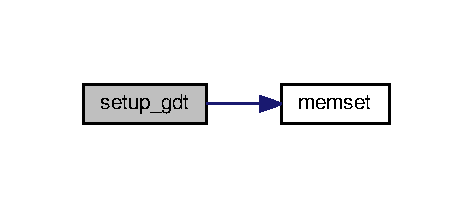
\includegraphics[width=227pt]{cpu__settings_8h_a1dee95fcf5b686585b942ed28875b442_cgraph}
\end{center}
\end{figure}
\mbox{\Hypertarget{cpu__settings_8h_a9782031a7d6cb759022b58789382f5eb}\label{cpu__settings_8h_a9782031a7d6cb759022b58789382f5eb}} 
\index{cpu\+\_\+settings.\+h@{cpu\+\_\+settings.\+h}!setup\+\_\+idt@{setup\+\_\+idt}}
\index{setup\+\_\+idt@{setup\+\_\+idt}!cpu\+\_\+settings.\+h@{cpu\+\_\+settings.\+h}}
\subsubsection{\texorpdfstring{setup\+\_\+idt()}{setup\_idt()}}
{\footnotesize\ttfamily void setup\+\_\+idt (\begin{DoxyParamCaption}\item[{void}]{ }\end{DoxyParamCaption})}



Setups the generic kernel\textquotesingle{}s I\+DT in memory and loads it in the I\+DT register. 

Setups a simple I\+DT for the kernel. Fills the entries in the I\+DT table by adding basic support to the x86 exception (interrutps 0 to 32). The rest of the interrupts are not set. Here is the call graph for this function\+:\nopagebreak
\begin{figure}[H]
\begin{center}
\leavevmode
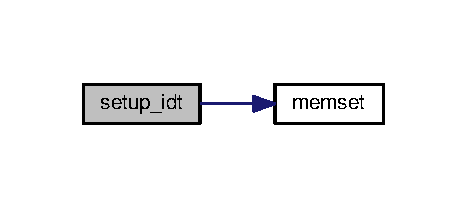
\includegraphics[width=224pt]{cpu__settings_8h_a9782031a7d6cb759022b58789382f5eb_cgraph}
\end{center}
\end{figure}
\mbox{\Hypertarget{cpu__settings_8h_aadd2bb249d145a23fefd086361c11ff2}\label{cpu__settings_8h_aadd2bb249d145a23fefd086361c11ff2}} 
\index{cpu\+\_\+settings.\+h@{cpu\+\_\+settings.\+h}!setup\+\_\+tss@{setup\+\_\+tss}}
\index{setup\+\_\+tss@{setup\+\_\+tss}!cpu\+\_\+settings.\+h@{cpu\+\_\+settings.\+h}}
\subsubsection{\texorpdfstring{setup\+\_\+tss()}{setup\_tss()}}
{\footnotesize\ttfamily void setup\+\_\+tss (\begin{DoxyParamCaption}\item[{void}]{ }\end{DoxyParamCaption})}



Setups the main C\+PU T\+SS for the kernel. 

Initializes the main C\+PU\textquotesingle{}s T\+SS with kernel settings in memory and loads it in the T\+SS register. Here is the call graph for this function\+:\nopagebreak
\begin{figure}[H]
\begin{center}
\leavevmode
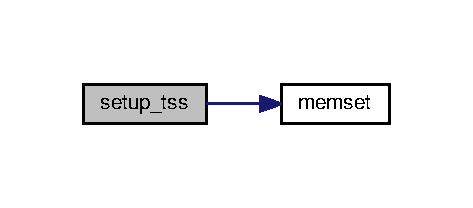
\includegraphics[width=227pt]{cpu__settings_8h_aadd2bb249d145a23fefd086361c11ff2_cgraph}
\end{center}
\end{figure}

\hypertarget{graphic_8h}{}\section{/home/alexy/\+Documents/\+Dev/\+R\+T\+L\+K\+I\+M/\+Source/\+Includes/\+Drivers/graphic.h File Reference}
\label{graphic_8h}\index{/home/alexy/\+Documents/\+Dev/\+R\+T\+L\+K\+I\+M/\+Source/\+Includes/\+Drivers/graphic.\+h@{/home/alexy/\+Documents/\+Dev/\+R\+T\+L\+K\+I\+M/\+Source/\+Includes/\+Drivers/graphic.\+h}}
{\ttfamily \#include $<$Lib/stdint.\+h$>$}\newline
{\ttfamily \#include $<$Lib/stddef.\+h$>$}\newline
Include dependency graph for graphic.\+h\+:\nopagebreak
\begin{figure}[H]
\begin{center}
\leavevmode
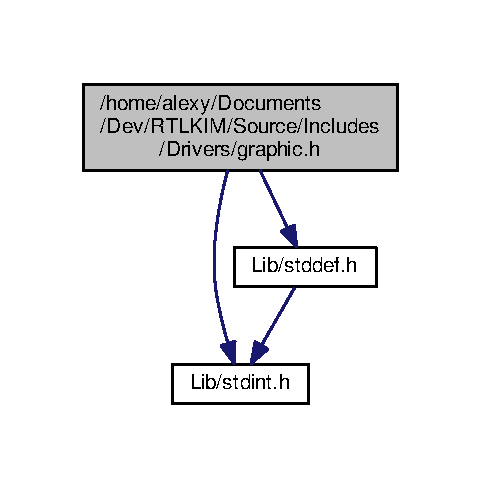
\includegraphics[width=231pt]{graphic_8h__incl}
\end{center}
\end{figure}
This graph shows which files directly or indirectly include this file\+:\nopagebreak
\begin{figure}[H]
\begin{center}
\leavevmode
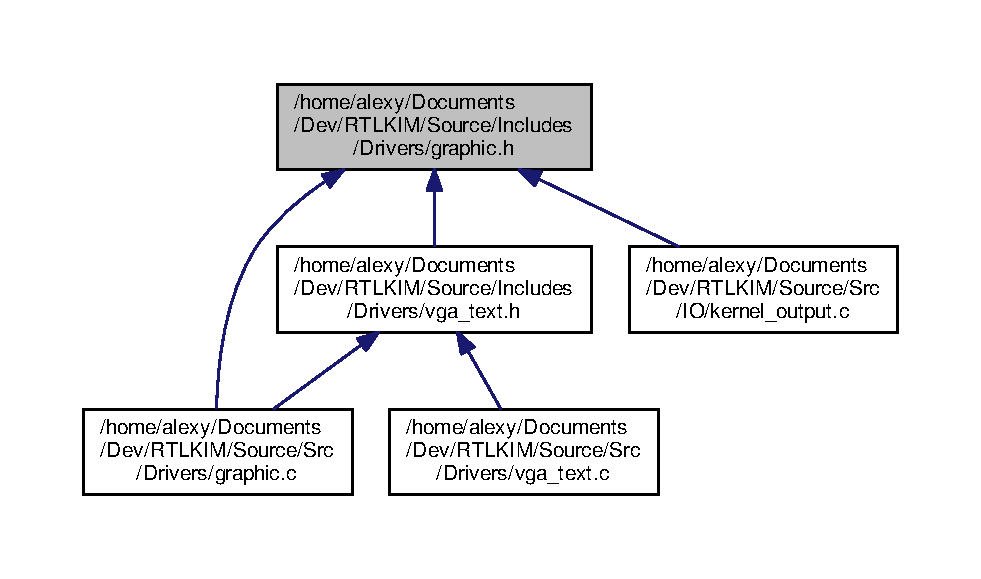
\includegraphics[width=350pt]{graphic_8h__dep__incl}
\end{center}
\end{figure}
\subsection*{Data Structures}
\begin{DoxyCompactItemize}
\item 
struct \hyperlink{structcursor}{cursor}
\item 
struct \hyperlink{structcolorscheme}{colorscheme}
\end{DoxyCompactItemize}
\subsection*{Macros}
\begin{DoxyCompactItemize}
\item 
\#define \hyperlink{graphic_8h_a632f1d66cbe05e1e1d5b4d61507f00f9}{V\+G\+A\+\_\+\+D\+R\+I\+V\+E\+R\+\_\+\+S\+E\+L\+E\+C\+T\+ED}~0x01
\item 
\#define \hyperlink{graphic_8h_abe82e4c033ebe532baf8193ea9f3f484}{V\+E\+S\+A\+\_\+\+D\+R\+I\+V\+E\+R\+\_\+\+S\+E\+L\+E\+C\+T\+ED}~0x02
\item 
\#define \hyperlink{graphic_8h_a0e5ebbe291d95cf1b8f1661252722fe0}{B\+G\+\_\+\+B\+L\+A\+CK}~0x00
\item 
\#define \hyperlink{graphic_8h_a9afd14c731aa8c62d9471913c1b23b9f}{B\+G\+\_\+\+B\+L\+UE}~0x10
\item 
\#define \hyperlink{graphic_8h_ac351fb4567ed6655a5b39769cc5dfd04}{B\+G\+\_\+\+G\+R\+E\+EN}~0x20
\item 
\#define \hyperlink{graphic_8h_a21ef237e1c4d69656729da4b34c31d8b}{B\+G\+\_\+\+C\+Y\+AN}~0x30
\item 
\#define \hyperlink{graphic_8h_ac317d04c219b630f9c36b0241d9d4be7}{B\+G\+\_\+\+R\+ED}~0x40
\item 
\#define \hyperlink{graphic_8h_ac08aa3f07e012f1b0edafa632d5300ba}{B\+G\+\_\+\+M\+A\+G\+E\+N\+TA}~0x50
\item 
\#define \hyperlink{graphic_8h_af0157c2ce04475a02bdcf45fe3e44a92}{B\+G\+\_\+\+B\+R\+O\+WN}~0x60
\item 
\#define \hyperlink{graphic_8h_a00213e74d04ed4d76a1339db5c26c70c}{B\+G\+\_\+\+G\+R\+EY}~0x70
\item 
\#define \hyperlink{graphic_8h_a01f446ce59cd9e70fb6bc16b20bc5350}{B\+G\+\_\+\+D\+A\+R\+K\+G\+R\+EY}~0x80
\item 
\#define \hyperlink{graphic_8h_a33397d5747fe9c2226f99478f17e9460}{B\+G\+\_\+\+B\+R\+I\+G\+H\+T\+B\+L\+UE}~0x90
\item 
\#define \hyperlink{graphic_8h_a5a6b2c6a82a458acd6bc3f3d0a03e715}{B\+G\+\_\+\+B\+R\+I\+G\+H\+T\+G\+R\+E\+EN}~0x\+A0
\item 
\#define \hyperlink{graphic_8h_a8f2c8dd03ac9198f30e40d14f8815069}{B\+G\+\_\+\+B\+R\+I\+G\+H\+T\+C\+Y\+AN}~0x\+B0
\item 
\#define \hyperlink{graphic_8h_a7b78f0791621cae1bfe50d99075ddafa}{B\+G\+\_\+\+B\+R\+I\+G\+H\+T\+R\+ED}~0x\+C0
\item 
\#define \hyperlink{graphic_8h_a1203ef2a5889b64e43d62efa8e52f890}{B\+G\+\_\+\+B\+R\+I\+G\+H\+T\+M\+A\+G\+E\+N\+TA}~0x\+D0
\item 
\#define \hyperlink{graphic_8h_ab31fe3e74b1137650d30ede5c9b86218}{B\+G\+\_\+\+Y\+E\+L\+L\+OW}~0x\+E0
\item 
\#define \hyperlink{graphic_8h_a6beded3f171517df3902c52f79f6fea2}{B\+G\+\_\+\+W\+H\+I\+TE}~0x\+F0
\item 
\#define \hyperlink{graphic_8h_a9b32d0a26f9909c5b63ccd474f56420e}{F\+G\+\_\+\+B\+L\+A\+CK}~0x00
\item 
\#define \hyperlink{graphic_8h_a4e411f6bd6ac8d6c2bd23d866c097e91}{F\+G\+\_\+\+B\+L\+UE}~0x01
\item 
\#define \hyperlink{graphic_8h_a0af1e03653ace4d21aebf3b2e03a6535}{F\+G\+\_\+\+G\+R\+E\+EN}~0x02
\item 
\#define \hyperlink{graphic_8h_afb40e6e076755308612ed6e18a34dbeb}{F\+G\+\_\+\+C\+Y\+AN}~0x03
\item 
\#define \hyperlink{graphic_8h_a1dc5215d084174df6f00a9267cec2f17}{F\+G\+\_\+\+R\+ED}~0x04
\item 
\#define \hyperlink{graphic_8h_aacf8f7d7b2a3f4ba0d0a131fcd1f1933}{F\+G\+\_\+\+M\+A\+G\+E\+N\+TA}~0x05
\item 
\#define \hyperlink{graphic_8h_a7f5f0a051433665586340a4c5db46a0e}{F\+G\+\_\+\+B\+R\+O\+WN}~0x06
\item 
\#define \hyperlink{graphic_8h_a5142f80dfa88eb9adc9d8acda8c492dd}{F\+G\+\_\+\+G\+R\+EY}~0x07
\item 
\#define \hyperlink{graphic_8h_a8e6ce3f2ce3e349ab09059a1de79f80f}{F\+G\+\_\+\+D\+A\+R\+K\+G\+R\+EY}~0x08
\item 
\#define \hyperlink{graphic_8h_a90e6477ae36af5a2b7a0d2035a69a96d}{F\+G\+\_\+\+B\+R\+I\+G\+H\+T\+B\+L\+UE}~0x09
\item 
\#define \hyperlink{graphic_8h_a2a3ef747fd07aa65ccbbe7b93e170d85}{F\+G\+\_\+\+B\+R\+I\+G\+H\+T\+G\+R\+E\+EN}~0x0A
\item 
\#define \hyperlink{graphic_8h_a2e66d2e78e23a9dfe8b00f00a9e34d93}{F\+G\+\_\+\+B\+R\+I\+G\+H\+T\+C\+Y\+AN}~0x0B
\item 
\#define \hyperlink{graphic_8h_a757d422eda569f40648fdb43eec745e8}{F\+G\+\_\+\+B\+R\+I\+G\+H\+T\+R\+ED}~0x0C
\item 
\#define \hyperlink{graphic_8h_a2b6ad4bee5d0fc64d8d8abd8f1d39bd8}{F\+G\+\_\+\+B\+R\+I\+G\+H\+T\+M\+A\+G\+E\+N\+TA}~0x0D
\item 
\#define \hyperlink{graphic_8h_a266aa539aa271da1b1f711d2413b1bfa}{F\+G\+\_\+\+Y\+E\+L\+L\+OW}~0x0E
\item 
\#define \hyperlink{graphic_8h_a7fbb956b9e769a1020c2eff1f6743857}{F\+G\+\_\+\+W\+H\+I\+TE}~0x0F
\end{DoxyCompactItemize}
\subsection*{Typedefs}
\begin{DoxyCompactItemize}
\item 
typedef enum \hyperlink{graphic_8h_a877a41e734f5020c27f9cb32db73ef8c}{G\+R\+A\+P\+H\+I\+C\+\_\+\+D\+R\+I\+V\+ER} \hyperlink{graphic_8h_a8731c83da869086e51c9576e7b24211b}{G\+R\+A\+P\+H\+I\+C\+\_\+\+D\+R\+I\+V\+E\+R\+\_\+E}
\item 
typedef struct \hyperlink{structcursor}{cursor} \hyperlink{graphic_8h_a2377a22e1ea925fc95c5ec7b5bea95f5}{cursor\+\_\+t}
\item 
typedef enum \hyperlink{graphic_8h_aee925ebfb72773b337e330bbdabdd604}{S\+C\+R\+O\+L\+L\+\_\+\+D\+I\+R\+E\+C\+T\+I\+ON} \hyperlink{graphic_8h_a223e9e8985b8d61206bd7628103b726f}{S\+C\+R\+O\+L\+L\+\_\+\+D\+I\+R\+E\+C\+T\+I\+O\+N\+\_\+E}
\item 
typedef struct \hyperlink{structcolorscheme}{colorscheme} \hyperlink{graphic_8h_ad71288aca9a1e3d064316c1072f04bb7}{colorscheme\+\_\+t}
\end{DoxyCompactItemize}
\subsection*{Enumerations}
\begin{DoxyCompactItemize}
\item 
enum \hyperlink{graphic_8h_a877a41e734f5020c27f9cb32db73ef8c}{G\+R\+A\+P\+H\+I\+C\+\_\+\+D\+R\+I\+V\+ER} \{ \hyperlink{graphic_8h_a877a41e734f5020c27f9cb32db73ef8ca7eba2e670e8c11b8afbb53c738a64652}{V\+G\+A\+\_\+\+D\+R\+I\+V\+ER} = V\+G\+A\+\_\+\+D\+R\+I\+V\+E\+R\+\_\+\+S\+E\+L\+E\+C\+T\+ED, 
\hyperlink{graphic_8h_a877a41e734f5020c27f9cb32db73ef8ca2c5c025596e0b99408d00d8efa6ccf8b}{V\+E\+S\+A\+\_\+\+D\+R\+I\+V\+ER} = V\+E\+S\+A\+\_\+\+D\+R\+I\+V\+E\+R\+\_\+\+S\+E\+L\+E\+C\+T\+ED
 \}
\item 
enum \hyperlink{graphic_8h_aee925ebfb72773b337e330bbdabdd604}{S\+C\+R\+O\+L\+L\+\_\+\+D\+I\+R\+E\+C\+T\+I\+ON} \{ \hyperlink{graphic_8h_aee925ebfb72773b337e330bbdabdd604a9d522bb191bf21bcaace5569ec49475d}{S\+C\+R\+O\+L\+L\+\_\+\+D\+O\+WN}, 
\hyperlink{graphic_8h_aee925ebfb72773b337e330bbdabdd604adc276c852fdda273d5091ee8e2ceb4ec}{S\+C\+R\+O\+L\+L\+\_\+\+UP}
 \}
\end{DoxyCompactItemize}
\subsection*{Functions}
\begin{DoxyCompactItemize}
\item 
void \hyperlink{graphic_8h_a456270cf61ec7c16f59eec8ce776b37f}{set\+\_\+selected\+\_\+driver} (const \hyperlink{graphic_8h_a8731c83da869086e51c9576e7b24211b}{G\+R\+A\+P\+H\+I\+C\+\_\+\+D\+R\+I\+V\+E\+R\+\_\+E} sel)
\item 
void \hyperlink{graphic_8h_abc40cd622f423abf44084c8f8595f57f}{clear\+\_\+screen} (void)
\item 
\hyperlink{stddef_8h_a51557cb52bbb9ee9d55aab5b9b16c3d0}{O\+S\+\_\+\+R\+E\+T\+U\+R\+N\+\_\+E} \hyperlink{graphic_8h_a839c7aea0eb4885f5270c20d95c6f224}{put\+\_\+cursor\+\_\+at} (const \hyperlink{stdint_8h_a324c5d28c0d82f502a234ab99efac87a}{uint32\+\_\+t} line, const \hyperlink{stdint_8h_a324c5d28c0d82f502a234ab99efac87a}{uint32\+\_\+t} column)
\item 
\hyperlink{stddef_8h_a51557cb52bbb9ee9d55aab5b9b16c3d0}{O\+S\+\_\+\+R\+E\+T\+U\+R\+N\+\_\+E} \hyperlink{graphic_8h_abc1ced411d18368a3d17840ca9fc5512}{save\+\_\+cursor} (\hyperlink{graphic_8h_a2377a22e1ea925fc95c5ec7b5bea95f5}{cursor\+\_\+t} $\ast$buffer)
\item 
\hyperlink{stddef_8h_a51557cb52bbb9ee9d55aab5b9b16c3d0}{O\+S\+\_\+\+R\+E\+T\+U\+R\+N\+\_\+E} \hyperlink{graphic_8h_a1e87d66055abaea40fde313f1446aa37}{restore\+\_\+cursor} (const \hyperlink{graphic_8h_a2377a22e1ea925fc95c5ec7b5bea95f5}{cursor\+\_\+t} buffer)
\item 
void \hyperlink{graphic_8h_a09a41c5d72f945277e7ce67b07a8dd79}{scroll} (const \hyperlink{graphic_8h_a223e9e8985b8d61206bd7628103b726f}{S\+C\+R\+O\+L\+L\+\_\+\+D\+I\+R\+E\+C\+T\+I\+O\+N\+\_\+E} direction, const \hyperlink{stdint_8h_a324c5d28c0d82f502a234ab99efac87a}{uint32\+\_\+t} lines\+\_\+count)
\item 
void \hyperlink{graphic_8h_ab818d1480fd08b89d113e7951d139635}{set\+\_\+color\+\_\+scheme} (\hyperlink{graphic_8h_ad71288aca9a1e3d064316c1072f04bb7}{colorscheme\+\_\+t} color\+\_\+scheme)
\item 
\hyperlink{stddef_8h_a51557cb52bbb9ee9d55aab5b9b16c3d0}{O\+S\+\_\+\+R\+E\+T\+U\+R\+N\+\_\+E} \hyperlink{graphic_8h_a2233243d20d491dfcb4d9a5106ff53e6}{save\+\_\+color\+\_\+scheme} (\hyperlink{graphic_8h_ad71288aca9a1e3d064316c1072f04bb7}{colorscheme\+\_\+t} $\ast$buffer)
\item 
void \hyperlink{graphic_8h_ad985618911547ca61e84432fe18e5b8c}{screen\+\_\+put\+\_\+string} (const char $\ast$str)
\item 
void \hyperlink{graphic_8h_a38db267eb855286bed377c7dd921acb8}{screen\+\_\+put\+\_\+char} (const char character)
\item 
void \hyperlink{graphic_8h_a71625f77c43e97e5c5a8444877162556}{console\+\_\+write\+\_\+keyboard} (const char $\ast$str, const \hyperlink{stdint_8h_a324c5d28c0d82f502a234ab99efac87a}{uint32\+\_\+t} len)
\end{DoxyCompactItemize}


\subsection{Macro Definition Documentation}
\mbox{\Hypertarget{graphic_8h_a0e5ebbe291d95cf1b8f1661252722fe0}\label{graphic_8h_a0e5ebbe291d95cf1b8f1661252722fe0}} 
\index{graphic.\+h@{graphic.\+h}!B\+G\+\_\+\+B\+L\+A\+CK@{B\+G\+\_\+\+B\+L\+A\+CK}}
\index{B\+G\+\_\+\+B\+L\+A\+CK@{B\+G\+\_\+\+B\+L\+A\+CK}!graphic.\+h@{graphic.\+h}}
\subsubsection{\texorpdfstring{B\+G\+\_\+\+B\+L\+A\+CK}{BG\_BLACK}}
{\footnotesize\ttfamily \#define B\+G\+\_\+\+B\+L\+A\+CK~0x00}

\mbox{\Hypertarget{graphic_8h_a9afd14c731aa8c62d9471913c1b23b9f}\label{graphic_8h_a9afd14c731aa8c62d9471913c1b23b9f}} 
\index{graphic.\+h@{graphic.\+h}!B\+G\+\_\+\+B\+L\+UE@{B\+G\+\_\+\+B\+L\+UE}}
\index{B\+G\+\_\+\+B\+L\+UE@{B\+G\+\_\+\+B\+L\+UE}!graphic.\+h@{graphic.\+h}}
\subsubsection{\texorpdfstring{B\+G\+\_\+\+B\+L\+UE}{BG\_BLUE}}
{\footnotesize\ttfamily \#define B\+G\+\_\+\+B\+L\+UE~0x10}

\mbox{\Hypertarget{graphic_8h_a33397d5747fe9c2226f99478f17e9460}\label{graphic_8h_a33397d5747fe9c2226f99478f17e9460}} 
\index{graphic.\+h@{graphic.\+h}!B\+G\+\_\+\+B\+R\+I\+G\+H\+T\+B\+L\+UE@{B\+G\+\_\+\+B\+R\+I\+G\+H\+T\+B\+L\+UE}}
\index{B\+G\+\_\+\+B\+R\+I\+G\+H\+T\+B\+L\+UE@{B\+G\+\_\+\+B\+R\+I\+G\+H\+T\+B\+L\+UE}!graphic.\+h@{graphic.\+h}}
\subsubsection{\texorpdfstring{B\+G\+\_\+\+B\+R\+I\+G\+H\+T\+B\+L\+UE}{BG\_BRIGHTBLUE}}
{\footnotesize\ttfamily \#define B\+G\+\_\+\+B\+R\+I\+G\+H\+T\+B\+L\+UE~0x90}

\mbox{\Hypertarget{graphic_8h_a8f2c8dd03ac9198f30e40d14f8815069}\label{graphic_8h_a8f2c8dd03ac9198f30e40d14f8815069}} 
\index{graphic.\+h@{graphic.\+h}!B\+G\+\_\+\+B\+R\+I\+G\+H\+T\+C\+Y\+AN@{B\+G\+\_\+\+B\+R\+I\+G\+H\+T\+C\+Y\+AN}}
\index{B\+G\+\_\+\+B\+R\+I\+G\+H\+T\+C\+Y\+AN@{B\+G\+\_\+\+B\+R\+I\+G\+H\+T\+C\+Y\+AN}!graphic.\+h@{graphic.\+h}}
\subsubsection{\texorpdfstring{B\+G\+\_\+\+B\+R\+I\+G\+H\+T\+C\+Y\+AN}{BG\_BRIGHTCYAN}}
{\footnotesize\ttfamily \#define B\+G\+\_\+\+B\+R\+I\+G\+H\+T\+C\+Y\+AN~0x\+B0}

\mbox{\Hypertarget{graphic_8h_a5a6b2c6a82a458acd6bc3f3d0a03e715}\label{graphic_8h_a5a6b2c6a82a458acd6bc3f3d0a03e715}} 
\index{graphic.\+h@{graphic.\+h}!B\+G\+\_\+\+B\+R\+I\+G\+H\+T\+G\+R\+E\+EN@{B\+G\+\_\+\+B\+R\+I\+G\+H\+T\+G\+R\+E\+EN}}
\index{B\+G\+\_\+\+B\+R\+I\+G\+H\+T\+G\+R\+E\+EN@{B\+G\+\_\+\+B\+R\+I\+G\+H\+T\+G\+R\+E\+EN}!graphic.\+h@{graphic.\+h}}
\subsubsection{\texorpdfstring{B\+G\+\_\+\+B\+R\+I\+G\+H\+T\+G\+R\+E\+EN}{BG\_BRIGHTGREEN}}
{\footnotesize\ttfamily \#define B\+G\+\_\+\+B\+R\+I\+G\+H\+T\+G\+R\+E\+EN~0x\+A0}

\mbox{\Hypertarget{graphic_8h_a1203ef2a5889b64e43d62efa8e52f890}\label{graphic_8h_a1203ef2a5889b64e43d62efa8e52f890}} 
\index{graphic.\+h@{graphic.\+h}!B\+G\+\_\+\+B\+R\+I\+G\+H\+T\+M\+A\+G\+E\+N\+TA@{B\+G\+\_\+\+B\+R\+I\+G\+H\+T\+M\+A\+G\+E\+N\+TA}}
\index{B\+G\+\_\+\+B\+R\+I\+G\+H\+T\+M\+A\+G\+E\+N\+TA@{B\+G\+\_\+\+B\+R\+I\+G\+H\+T\+M\+A\+G\+E\+N\+TA}!graphic.\+h@{graphic.\+h}}
\subsubsection{\texorpdfstring{B\+G\+\_\+\+B\+R\+I\+G\+H\+T\+M\+A\+G\+E\+N\+TA}{BG\_BRIGHTMAGENTA}}
{\footnotesize\ttfamily \#define B\+G\+\_\+\+B\+R\+I\+G\+H\+T\+M\+A\+G\+E\+N\+TA~0x\+D0}

\mbox{\Hypertarget{graphic_8h_a7b78f0791621cae1bfe50d99075ddafa}\label{graphic_8h_a7b78f0791621cae1bfe50d99075ddafa}} 
\index{graphic.\+h@{graphic.\+h}!B\+G\+\_\+\+B\+R\+I\+G\+H\+T\+R\+ED@{B\+G\+\_\+\+B\+R\+I\+G\+H\+T\+R\+ED}}
\index{B\+G\+\_\+\+B\+R\+I\+G\+H\+T\+R\+ED@{B\+G\+\_\+\+B\+R\+I\+G\+H\+T\+R\+ED}!graphic.\+h@{graphic.\+h}}
\subsubsection{\texorpdfstring{B\+G\+\_\+\+B\+R\+I\+G\+H\+T\+R\+ED}{BG\_BRIGHTRED}}
{\footnotesize\ttfamily \#define B\+G\+\_\+\+B\+R\+I\+G\+H\+T\+R\+ED~0x\+C0}

\mbox{\Hypertarget{graphic_8h_af0157c2ce04475a02bdcf45fe3e44a92}\label{graphic_8h_af0157c2ce04475a02bdcf45fe3e44a92}} 
\index{graphic.\+h@{graphic.\+h}!B\+G\+\_\+\+B\+R\+O\+WN@{B\+G\+\_\+\+B\+R\+O\+WN}}
\index{B\+G\+\_\+\+B\+R\+O\+WN@{B\+G\+\_\+\+B\+R\+O\+WN}!graphic.\+h@{graphic.\+h}}
\subsubsection{\texorpdfstring{B\+G\+\_\+\+B\+R\+O\+WN}{BG\_BROWN}}
{\footnotesize\ttfamily \#define B\+G\+\_\+\+B\+R\+O\+WN~0x60}

\mbox{\Hypertarget{graphic_8h_a21ef237e1c4d69656729da4b34c31d8b}\label{graphic_8h_a21ef237e1c4d69656729da4b34c31d8b}} 
\index{graphic.\+h@{graphic.\+h}!B\+G\+\_\+\+C\+Y\+AN@{B\+G\+\_\+\+C\+Y\+AN}}
\index{B\+G\+\_\+\+C\+Y\+AN@{B\+G\+\_\+\+C\+Y\+AN}!graphic.\+h@{graphic.\+h}}
\subsubsection{\texorpdfstring{B\+G\+\_\+\+C\+Y\+AN}{BG\_CYAN}}
{\footnotesize\ttfamily \#define B\+G\+\_\+\+C\+Y\+AN~0x30}

\mbox{\Hypertarget{graphic_8h_a01f446ce59cd9e70fb6bc16b20bc5350}\label{graphic_8h_a01f446ce59cd9e70fb6bc16b20bc5350}} 
\index{graphic.\+h@{graphic.\+h}!B\+G\+\_\+\+D\+A\+R\+K\+G\+R\+EY@{B\+G\+\_\+\+D\+A\+R\+K\+G\+R\+EY}}
\index{B\+G\+\_\+\+D\+A\+R\+K\+G\+R\+EY@{B\+G\+\_\+\+D\+A\+R\+K\+G\+R\+EY}!graphic.\+h@{graphic.\+h}}
\subsubsection{\texorpdfstring{B\+G\+\_\+\+D\+A\+R\+K\+G\+R\+EY}{BG\_DARKGREY}}
{\footnotesize\ttfamily \#define B\+G\+\_\+\+D\+A\+R\+K\+G\+R\+EY~0x80}

\mbox{\Hypertarget{graphic_8h_ac351fb4567ed6655a5b39769cc5dfd04}\label{graphic_8h_ac351fb4567ed6655a5b39769cc5dfd04}} 
\index{graphic.\+h@{graphic.\+h}!B\+G\+\_\+\+G\+R\+E\+EN@{B\+G\+\_\+\+G\+R\+E\+EN}}
\index{B\+G\+\_\+\+G\+R\+E\+EN@{B\+G\+\_\+\+G\+R\+E\+EN}!graphic.\+h@{graphic.\+h}}
\subsubsection{\texorpdfstring{B\+G\+\_\+\+G\+R\+E\+EN}{BG\_GREEN}}
{\footnotesize\ttfamily \#define B\+G\+\_\+\+G\+R\+E\+EN~0x20}

\mbox{\Hypertarget{graphic_8h_a00213e74d04ed4d76a1339db5c26c70c}\label{graphic_8h_a00213e74d04ed4d76a1339db5c26c70c}} 
\index{graphic.\+h@{graphic.\+h}!B\+G\+\_\+\+G\+R\+EY@{B\+G\+\_\+\+G\+R\+EY}}
\index{B\+G\+\_\+\+G\+R\+EY@{B\+G\+\_\+\+G\+R\+EY}!graphic.\+h@{graphic.\+h}}
\subsubsection{\texorpdfstring{B\+G\+\_\+\+G\+R\+EY}{BG\_GREY}}
{\footnotesize\ttfamily \#define B\+G\+\_\+\+G\+R\+EY~0x70}

\mbox{\Hypertarget{graphic_8h_ac08aa3f07e012f1b0edafa632d5300ba}\label{graphic_8h_ac08aa3f07e012f1b0edafa632d5300ba}} 
\index{graphic.\+h@{graphic.\+h}!B\+G\+\_\+\+M\+A\+G\+E\+N\+TA@{B\+G\+\_\+\+M\+A\+G\+E\+N\+TA}}
\index{B\+G\+\_\+\+M\+A\+G\+E\+N\+TA@{B\+G\+\_\+\+M\+A\+G\+E\+N\+TA}!graphic.\+h@{graphic.\+h}}
\subsubsection{\texorpdfstring{B\+G\+\_\+\+M\+A\+G\+E\+N\+TA}{BG\_MAGENTA}}
{\footnotesize\ttfamily \#define B\+G\+\_\+\+M\+A\+G\+E\+N\+TA~0x50}

\mbox{\Hypertarget{graphic_8h_ac317d04c219b630f9c36b0241d9d4be7}\label{graphic_8h_ac317d04c219b630f9c36b0241d9d4be7}} 
\index{graphic.\+h@{graphic.\+h}!B\+G\+\_\+\+R\+ED@{B\+G\+\_\+\+R\+ED}}
\index{B\+G\+\_\+\+R\+ED@{B\+G\+\_\+\+R\+ED}!graphic.\+h@{graphic.\+h}}
\subsubsection{\texorpdfstring{B\+G\+\_\+\+R\+ED}{BG\_RED}}
{\footnotesize\ttfamily \#define B\+G\+\_\+\+R\+ED~0x40}

\mbox{\Hypertarget{graphic_8h_a6beded3f171517df3902c52f79f6fea2}\label{graphic_8h_a6beded3f171517df3902c52f79f6fea2}} 
\index{graphic.\+h@{graphic.\+h}!B\+G\+\_\+\+W\+H\+I\+TE@{B\+G\+\_\+\+W\+H\+I\+TE}}
\index{B\+G\+\_\+\+W\+H\+I\+TE@{B\+G\+\_\+\+W\+H\+I\+TE}!graphic.\+h@{graphic.\+h}}
\subsubsection{\texorpdfstring{B\+G\+\_\+\+W\+H\+I\+TE}{BG\_WHITE}}
{\footnotesize\ttfamily \#define B\+G\+\_\+\+W\+H\+I\+TE~0x\+F0}

\mbox{\Hypertarget{graphic_8h_ab31fe3e74b1137650d30ede5c9b86218}\label{graphic_8h_ab31fe3e74b1137650d30ede5c9b86218}} 
\index{graphic.\+h@{graphic.\+h}!B\+G\+\_\+\+Y\+E\+L\+L\+OW@{B\+G\+\_\+\+Y\+E\+L\+L\+OW}}
\index{B\+G\+\_\+\+Y\+E\+L\+L\+OW@{B\+G\+\_\+\+Y\+E\+L\+L\+OW}!graphic.\+h@{graphic.\+h}}
\subsubsection{\texorpdfstring{B\+G\+\_\+\+Y\+E\+L\+L\+OW}{BG\_YELLOW}}
{\footnotesize\ttfamily \#define B\+G\+\_\+\+Y\+E\+L\+L\+OW~0x\+E0}

\mbox{\Hypertarget{graphic_8h_a9b32d0a26f9909c5b63ccd474f56420e}\label{graphic_8h_a9b32d0a26f9909c5b63ccd474f56420e}} 
\index{graphic.\+h@{graphic.\+h}!F\+G\+\_\+\+B\+L\+A\+CK@{F\+G\+\_\+\+B\+L\+A\+CK}}
\index{F\+G\+\_\+\+B\+L\+A\+CK@{F\+G\+\_\+\+B\+L\+A\+CK}!graphic.\+h@{graphic.\+h}}
\subsubsection{\texorpdfstring{F\+G\+\_\+\+B\+L\+A\+CK}{FG\_BLACK}}
{\footnotesize\ttfamily \#define F\+G\+\_\+\+B\+L\+A\+CK~0x00}

\mbox{\Hypertarget{graphic_8h_a4e411f6bd6ac8d6c2bd23d866c097e91}\label{graphic_8h_a4e411f6bd6ac8d6c2bd23d866c097e91}} 
\index{graphic.\+h@{graphic.\+h}!F\+G\+\_\+\+B\+L\+UE@{F\+G\+\_\+\+B\+L\+UE}}
\index{F\+G\+\_\+\+B\+L\+UE@{F\+G\+\_\+\+B\+L\+UE}!graphic.\+h@{graphic.\+h}}
\subsubsection{\texorpdfstring{F\+G\+\_\+\+B\+L\+UE}{FG\_BLUE}}
{\footnotesize\ttfamily \#define F\+G\+\_\+\+B\+L\+UE~0x01}

\mbox{\Hypertarget{graphic_8h_a90e6477ae36af5a2b7a0d2035a69a96d}\label{graphic_8h_a90e6477ae36af5a2b7a0d2035a69a96d}} 
\index{graphic.\+h@{graphic.\+h}!F\+G\+\_\+\+B\+R\+I\+G\+H\+T\+B\+L\+UE@{F\+G\+\_\+\+B\+R\+I\+G\+H\+T\+B\+L\+UE}}
\index{F\+G\+\_\+\+B\+R\+I\+G\+H\+T\+B\+L\+UE@{F\+G\+\_\+\+B\+R\+I\+G\+H\+T\+B\+L\+UE}!graphic.\+h@{graphic.\+h}}
\subsubsection{\texorpdfstring{F\+G\+\_\+\+B\+R\+I\+G\+H\+T\+B\+L\+UE}{FG\_BRIGHTBLUE}}
{\footnotesize\ttfamily \#define F\+G\+\_\+\+B\+R\+I\+G\+H\+T\+B\+L\+UE~0x09}

\mbox{\Hypertarget{graphic_8h_a2e66d2e78e23a9dfe8b00f00a9e34d93}\label{graphic_8h_a2e66d2e78e23a9dfe8b00f00a9e34d93}} 
\index{graphic.\+h@{graphic.\+h}!F\+G\+\_\+\+B\+R\+I\+G\+H\+T\+C\+Y\+AN@{F\+G\+\_\+\+B\+R\+I\+G\+H\+T\+C\+Y\+AN}}
\index{F\+G\+\_\+\+B\+R\+I\+G\+H\+T\+C\+Y\+AN@{F\+G\+\_\+\+B\+R\+I\+G\+H\+T\+C\+Y\+AN}!graphic.\+h@{graphic.\+h}}
\subsubsection{\texorpdfstring{F\+G\+\_\+\+B\+R\+I\+G\+H\+T\+C\+Y\+AN}{FG\_BRIGHTCYAN}}
{\footnotesize\ttfamily \#define F\+G\+\_\+\+B\+R\+I\+G\+H\+T\+C\+Y\+AN~0x0B}

\mbox{\Hypertarget{graphic_8h_a2a3ef747fd07aa65ccbbe7b93e170d85}\label{graphic_8h_a2a3ef747fd07aa65ccbbe7b93e170d85}} 
\index{graphic.\+h@{graphic.\+h}!F\+G\+\_\+\+B\+R\+I\+G\+H\+T\+G\+R\+E\+EN@{F\+G\+\_\+\+B\+R\+I\+G\+H\+T\+G\+R\+E\+EN}}
\index{F\+G\+\_\+\+B\+R\+I\+G\+H\+T\+G\+R\+E\+EN@{F\+G\+\_\+\+B\+R\+I\+G\+H\+T\+G\+R\+E\+EN}!graphic.\+h@{graphic.\+h}}
\subsubsection{\texorpdfstring{F\+G\+\_\+\+B\+R\+I\+G\+H\+T\+G\+R\+E\+EN}{FG\_BRIGHTGREEN}}
{\footnotesize\ttfamily \#define F\+G\+\_\+\+B\+R\+I\+G\+H\+T\+G\+R\+E\+EN~0x0A}

\mbox{\Hypertarget{graphic_8h_a2b6ad4bee5d0fc64d8d8abd8f1d39bd8}\label{graphic_8h_a2b6ad4bee5d0fc64d8d8abd8f1d39bd8}} 
\index{graphic.\+h@{graphic.\+h}!F\+G\+\_\+\+B\+R\+I\+G\+H\+T\+M\+A\+G\+E\+N\+TA@{F\+G\+\_\+\+B\+R\+I\+G\+H\+T\+M\+A\+G\+E\+N\+TA}}
\index{F\+G\+\_\+\+B\+R\+I\+G\+H\+T\+M\+A\+G\+E\+N\+TA@{F\+G\+\_\+\+B\+R\+I\+G\+H\+T\+M\+A\+G\+E\+N\+TA}!graphic.\+h@{graphic.\+h}}
\subsubsection{\texorpdfstring{F\+G\+\_\+\+B\+R\+I\+G\+H\+T\+M\+A\+G\+E\+N\+TA}{FG\_BRIGHTMAGENTA}}
{\footnotesize\ttfamily \#define F\+G\+\_\+\+B\+R\+I\+G\+H\+T\+M\+A\+G\+E\+N\+TA~0x0D}

\mbox{\Hypertarget{graphic_8h_a757d422eda569f40648fdb43eec745e8}\label{graphic_8h_a757d422eda569f40648fdb43eec745e8}} 
\index{graphic.\+h@{graphic.\+h}!F\+G\+\_\+\+B\+R\+I\+G\+H\+T\+R\+ED@{F\+G\+\_\+\+B\+R\+I\+G\+H\+T\+R\+ED}}
\index{F\+G\+\_\+\+B\+R\+I\+G\+H\+T\+R\+ED@{F\+G\+\_\+\+B\+R\+I\+G\+H\+T\+R\+ED}!graphic.\+h@{graphic.\+h}}
\subsubsection{\texorpdfstring{F\+G\+\_\+\+B\+R\+I\+G\+H\+T\+R\+ED}{FG\_BRIGHTRED}}
{\footnotesize\ttfamily \#define F\+G\+\_\+\+B\+R\+I\+G\+H\+T\+R\+ED~0x0C}

\mbox{\Hypertarget{graphic_8h_a7f5f0a051433665586340a4c5db46a0e}\label{graphic_8h_a7f5f0a051433665586340a4c5db46a0e}} 
\index{graphic.\+h@{graphic.\+h}!F\+G\+\_\+\+B\+R\+O\+WN@{F\+G\+\_\+\+B\+R\+O\+WN}}
\index{F\+G\+\_\+\+B\+R\+O\+WN@{F\+G\+\_\+\+B\+R\+O\+WN}!graphic.\+h@{graphic.\+h}}
\subsubsection{\texorpdfstring{F\+G\+\_\+\+B\+R\+O\+WN}{FG\_BROWN}}
{\footnotesize\ttfamily \#define F\+G\+\_\+\+B\+R\+O\+WN~0x06}

\mbox{\Hypertarget{graphic_8h_afb40e6e076755308612ed6e18a34dbeb}\label{graphic_8h_afb40e6e076755308612ed6e18a34dbeb}} 
\index{graphic.\+h@{graphic.\+h}!F\+G\+\_\+\+C\+Y\+AN@{F\+G\+\_\+\+C\+Y\+AN}}
\index{F\+G\+\_\+\+C\+Y\+AN@{F\+G\+\_\+\+C\+Y\+AN}!graphic.\+h@{graphic.\+h}}
\subsubsection{\texorpdfstring{F\+G\+\_\+\+C\+Y\+AN}{FG\_CYAN}}
{\footnotesize\ttfamily \#define F\+G\+\_\+\+C\+Y\+AN~0x03}

\mbox{\Hypertarget{graphic_8h_a8e6ce3f2ce3e349ab09059a1de79f80f}\label{graphic_8h_a8e6ce3f2ce3e349ab09059a1de79f80f}} 
\index{graphic.\+h@{graphic.\+h}!F\+G\+\_\+\+D\+A\+R\+K\+G\+R\+EY@{F\+G\+\_\+\+D\+A\+R\+K\+G\+R\+EY}}
\index{F\+G\+\_\+\+D\+A\+R\+K\+G\+R\+EY@{F\+G\+\_\+\+D\+A\+R\+K\+G\+R\+EY}!graphic.\+h@{graphic.\+h}}
\subsubsection{\texorpdfstring{F\+G\+\_\+\+D\+A\+R\+K\+G\+R\+EY}{FG\_DARKGREY}}
{\footnotesize\ttfamily \#define F\+G\+\_\+\+D\+A\+R\+K\+G\+R\+EY~0x08}

\mbox{\Hypertarget{graphic_8h_a0af1e03653ace4d21aebf3b2e03a6535}\label{graphic_8h_a0af1e03653ace4d21aebf3b2e03a6535}} 
\index{graphic.\+h@{graphic.\+h}!F\+G\+\_\+\+G\+R\+E\+EN@{F\+G\+\_\+\+G\+R\+E\+EN}}
\index{F\+G\+\_\+\+G\+R\+E\+EN@{F\+G\+\_\+\+G\+R\+E\+EN}!graphic.\+h@{graphic.\+h}}
\subsubsection{\texorpdfstring{F\+G\+\_\+\+G\+R\+E\+EN}{FG\_GREEN}}
{\footnotesize\ttfamily \#define F\+G\+\_\+\+G\+R\+E\+EN~0x02}

\mbox{\Hypertarget{graphic_8h_a5142f80dfa88eb9adc9d8acda8c492dd}\label{graphic_8h_a5142f80dfa88eb9adc9d8acda8c492dd}} 
\index{graphic.\+h@{graphic.\+h}!F\+G\+\_\+\+G\+R\+EY@{F\+G\+\_\+\+G\+R\+EY}}
\index{F\+G\+\_\+\+G\+R\+EY@{F\+G\+\_\+\+G\+R\+EY}!graphic.\+h@{graphic.\+h}}
\subsubsection{\texorpdfstring{F\+G\+\_\+\+G\+R\+EY}{FG\_GREY}}
{\footnotesize\ttfamily \#define F\+G\+\_\+\+G\+R\+EY~0x07}

\mbox{\Hypertarget{graphic_8h_aacf8f7d7b2a3f4ba0d0a131fcd1f1933}\label{graphic_8h_aacf8f7d7b2a3f4ba0d0a131fcd1f1933}} 
\index{graphic.\+h@{graphic.\+h}!F\+G\+\_\+\+M\+A\+G\+E\+N\+TA@{F\+G\+\_\+\+M\+A\+G\+E\+N\+TA}}
\index{F\+G\+\_\+\+M\+A\+G\+E\+N\+TA@{F\+G\+\_\+\+M\+A\+G\+E\+N\+TA}!graphic.\+h@{graphic.\+h}}
\subsubsection{\texorpdfstring{F\+G\+\_\+\+M\+A\+G\+E\+N\+TA}{FG\_MAGENTA}}
{\footnotesize\ttfamily \#define F\+G\+\_\+\+M\+A\+G\+E\+N\+TA~0x05}

\mbox{\Hypertarget{graphic_8h_a1dc5215d084174df6f00a9267cec2f17}\label{graphic_8h_a1dc5215d084174df6f00a9267cec2f17}} 
\index{graphic.\+h@{graphic.\+h}!F\+G\+\_\+\+R\+ED@{F\+G\+\_\+\+R\+ED}}
\index{F\+G\+\_\+\+R\+ED@{F\+G\+\_\+\+R\+ED}!graphic.\+h@{graphic.\+h}}
\subsubsection{\texorpdfstring{F\+G\+\_\+\+R\+ED}{FG\_RED}}
{\footnotesize\ttfamily \#define F\+G\+\_\+\+R\+ED~0x04}

\mbox{\Hypertarget{graphic_8h_a7fbb956b9e769a1020c2eff1f6743857}\label{graphic_8h_a7fbb956b9e769a1020c2eff1f6743857}} 
\index{graphic.\+h@{graphic.\+h}!F\+G\+\_\+\+W\+H\+I\+TE@{F\+G\+\_\+\+W\+H\+I\+TE}}
\index{F\+G\+\_\+\+W\+H\+I\+TE@{F\+G\+\_\+\+W\+H\+I\+TE}!graphic.\+h@{graphic.\+h}}
\subsubsection{\texorpdfstring{F\+G\+\_\+\+W\+H\+I\+TE}{FG\_WHITE}}
{\footnotesize\ttfamily \#define F\+G\+\_\+\+W\+H\+I\+TE~0x0F}

\mbox{\Hypertarget{graphic_8h_a266aa539aa271da1b1f711d2413b1bfa}\label{graphic_8h_a266aa539aa271da1b1f711d2413b1bfa}} 
\index{graphic.\+h@{graphic.\+h}!F\+G\+\_\+\+Y\+E\+L\+L\+OW@{F\+G\+\_\+\+Y\+E\+L\+L\+OW}}
\index{F\+G\+\_\+\+Y\+E\+L\+L\+OW@{F\+G\+\_\+\+Y\+E\+L\+L\+OW}!graphic.\+h@{graphic.\+h}}
\subsubsection{\texorpdfstring{F\+G\+\_\+\+Y\+E\+L\+L\+OW}{FG\_YELLOW}}
{\footnotesize\ttfamily \#define F\+G\+\_\+\+Y\+E\+L\+L\+OW~0x0E}

\mbox{\Hypertarget{graphic_8h_abe82e4c033ebe532baf8193ea9f3f484}\label{graphic_8h_abe82e4c033ebe532baf8193ea9f3f484}} 
\index{graphic.\+h@{graphic.\+h}!V\+E\+S\+A\+\_\+\+D\+R\+I\+V\+E\+R\+\_\+\+S\+E\+L\+E\+C\+T\+ED@{V\+E\+S\+A\+\_\+\+D\+R\+I\+V\+E\+R\+\_\+\+S\+E\+L\+E\+C\+T\+ED}}
\index{V\+E\+S\+A\+\_\+\+D\+R\+I\+V\+E\+R\+\_\+\+S\+E\+L\+E\+C\+T\+ED@{V\+E\+S\+A\+\_\+\+D\+R\+I\+V\+E\+R\+\_\+\+S\+E\+L\+E\+C\+T\+ED}!graphic.\+h@{graphic.\+h}}
\subsubsection{\texorpdfstring{V\+E\+S\+A\+\_\+\+D\+R\+I\+V\+E\+R\+\_\+\+S\+E\+L\+E\+C\+T\+ED}{VESA\_DRIVER\_SELECTED}}
{\footnotesize\ttfamily \#define V\+E\+S\+A\+\_\+\+D\+R\+I\+V\+E\+R\+\_\+\+S\+E\+L\+E\+C\+T\+ED~0x02}

\mbox{\Hypertarget{graphic_8h_a632f1d66cbe05e1e1d5b4d61507f00f9}\label{graphic_8h_a632f1d66cbe05e1e1d5b4d61507f00f9}} 
\index{graphic.\+h@{graphic.\+h}!V\+G\+A\+\_\+\+D\+R\+I\+V\+E\+R\+\_\+\+S\+E\+L\+E\+C\+T\+ED@{V\+G\+A\+\_\+\+D\+R\+I\+V\+E\+R\+\_\+\+S\+E\+L\+E\+C\+T\+ED}}
\index{V\+G\+A\+\_\+\+D\+R\+I\+V\+E\+R\+\_\+\+S\+E\+L\+E\+C\+T\+ED@{V\+G\+A\+\_\+\+D\+R\+I\+V\+E\+R\+\_\+\+S\+E\+L\+E\+C\+T\+ED}!graphic.\+h@{graphic.\+h}}
\subsubsection{\texorpdfstring{V\+G\+A\+\_\+\+D\+R\+I\+V\+E\+R\+\_\+\+S\+E\+L\+E\+C\+T\+ED}{VGA\_DRIVER\_SELECTED}}
{\footnotesize\ttfamily \#define V\+G\+A\+\_\+\+D\+R\+I\+V\+E\+R\+\_\+\+S\+E\+L\+E\+C\+T\+ED~0x01}



\subsection{Typedef Documentation}
\mbox{\Hypertarget{graphic_8h_ad71288aca9a1e3d064316c1072f04bb7}\label{graphic_8h_ad71288aca9a1e3d064316c1072f04bb7}} 
\index{graphic.\+h@{graphic.\+h}!colorscheme\+\_\+t@{colorscheme\+\_\+t}}
\index{colorscheme\+\_\+t@{colorscheme\+\_\+t}!graphic.\+h@{graphic.\+h}}
\subsubsection{\texorpdfstring{colorscheme\+\_\+t}{colorscheme\_t}}
{\footnotesize\ttfamily typedef struct \hyperlink{structcolorscheme}{colorscheme}  \hyperlink{graphic_8h_ad71288aca9a1e3d064316c1072f04bb7}{colorscheme\+\_\+t}}

\mbox{\Hypertarget{graphic_8h_a2377a22e1ea925fc95c5ec7b5bea95f5}\label{graphic_8h_a2377a22e1ea925fc95c5ec7b5bea95f5}} 
\index{graphic.\+h@{graphic.\+h}!cursor\+\_\+t@{cursor\+\_\+t}}
\index{cursor\+\_\+t@{cursor\+\_\+t}!graphic.\+h@{graphic.\+h}}
\subsubsection{\texorpdfstring{cursor\+\_\+t}{cursor\_t}}
{\footnotesize\ttfamily typedef struct \hyperlink{structcursor}{cursor}  \hyperlink{graphic_8h_a2377a22e1ea925fc95c5ec7b5bea95f5}{cursor\+\_\+t}}

\mbox{\Hypertarget{graphic_8h_a8731c83da869086e51c9576e7b24211b}\label{graphic_8h_a8731c83da869086e51c9576e7b24211b}} 
\index{graphic.\+h@{graphic.\+h}!G\+R\+A\+P\+H\+I\+C\+\_\+\+D\+R\+I\+V\+E\+R\+\_\+E@{G\+R\+A\+P\+H\+I\+C\+\_\+\+D\+R\+I\+V\+E\+R\+\_\+E}}
\index{G\+R\+A\+P\+H\+I\+C\+\_\+\+D\+R\+I\+V\+E\+R\+\_\+E@{G\+R\+A\+P\+H\+I\+C\+\_\+\+D\+R\+I\+V\+E\+R\+\_\+E}!graphic.\+h@{graphic.\+h}}
\subsubsection{\texorpdfstring{G\+R\+A\+P\+H\+I\+C\+\_\+\+D\+R\+I\+V\+E\+R\+\_\+E}{GRAPHIC\_DRIVER\_E}}
{\footnotesize\ttfamily typedef enum \hyperlink{graphic_8h_a877a41e734f5020c27f9cb32db73ef8c}{G\+R\+A\+P\+H\+I\+C\+\_\+\+D\+R\+I\+V\+ER}  \hyperlink{graphic_8h_a8731c83da869086e51c9576e7b24211b}{G\+R\+A\+P\+H\+I\+C\+\_\+\+D\+R\+I\+V\+E\+R\+\_\+E}}

\mbox{\Hypertarget{graphic_8h_a223e9e8985b8d61206bd7628103b726f}\label{graphic_8h_a223e9e8985b8d61206bd7628103b726f}} 
\index{graphic.\+h@{graphic.\+h}!S\+C\+R\+O\+L\+L\+\_\+\+D\+I\+R\+E\+C\+T\+I\+O\+N\+\_\+E@{S\+C\+R\+O\+L\+L\+\_\+\+D\+I\+R\+E\+C\+T\+I\+O\+N\+\_\+E}}
\index{S\+C\+R\+O\+L\+L\+\_\+\+D\+I\+R\+E\+C\+T\+I\+O\+N\+\_\+E@{S\+C\+R\+O\+L\+L\+\_\+\+D\+I\+R\+E\+C\+T\+I\+O\+N\+\_\+E}!graphic.\+h@{graphic.\+h}}
\subsubsection{\texorpdfstring{S\+C\+R\+O\+L\+L\+\_\+\+D\+I\+R\+E\+C\+T\+I\+O\+N\+\_\+E}{SCROLL\_DIRECTION\_E}}
{\footnotesize\ttfamily typedef enum \hyperlink{graphic_8h_aee925ebfb72773b337e330bbdabdd604}{S\+C\+R\+O\+L\+L\+\_\+\+D\+I\+R\+E\+C\+T\+I\+ON}  \hyperlink{graphic_8h_a223e9e8985b8d61206bd7628103b726f}{S\+C\+R\+O\+L\+L\+\_\+\+D\+I\+R\+E\+C\+T\+I\+O\+N\+\_\+E}}



\subsection{Enumeration Type Documentation}
\mbox{\Hypertarget{graphic_8h_a877a41e734f5020c27f9cb32db73ef8c}\label{graphic_8h_a877a41e734f5020c27f9cb32db73ef8c}} 
\index{graphic.\+h@{graphic.\+h}!G\+R\+A\+P\+H\+I\+C\+\_\+\+D\+R\+I\+V\+ER@{G\+R\+A\+P\+H\+I\+C\+\_\+\+D\+R\+I\+V\+ER}}
\index{G\+R\+A\+P\+H\+I\+C\+\_\+\+D\+R\+I\+V\+ER@{G\+R\+A\+P\+H\+I\+C\+\_\+\+D\+R\+I\+V\+ER}!graphic.\+h@{graphic.\+h}}
\subsubsection{\texorpdfstring{G\+R\+A\+P\+H\+I\+C\+\_\+\+D\+R\+I\+V\+ER}{GRAPHIC\_DRIVER}}
{\footnotesize\ttfamily enum \hyperlink{graphic_8h_a877a41e734f5020c27f9cb32db73ef8c}{G\+R\+A\+P\+H\+I\+C\+\_\+\+D\+R\+I\+V\+ER}}

\begin{DoxyEnumFields}{Enumerator}
\raisebox{\heightof{T}}[0pt][0pt]{\index{V\+G\+A\+\_\+\+D\+R\+I\+V\+ER@{V\+G\+A\+\_\+\+D\+R\+I\+V\+ER}!graphic.\+h@{graphic.\+h}}\index{graphic.\+h@{graphic.\+h}!V\+G\+A\+\_\+\+D\+R\+I\+V\+ER@{V\+G\+A\+\_\+\+D\+R\+I\+V\+ER}}}\mbox{\Hypertarget{graphic_8h_a877a41e734f5020c27f9cb32db73ef8ca7eba2e670e8c11b8afbb53c738a64652}\label{graphic_8h_a877a41e734f5020c27f9cb32db73ef8ca7eba2e670e8c11b8afbb53c738a64652}} 
V\+G\+A\+\_\+\+D\+R\+I\+V\+ER&\\
\hline

\raisebox{\heightof{T}}[0pt][0pt]{\index{V\+E\+S\+A\+\_\+\+D\+R\+I\+V\+ER@{V\+E\+S\+A\+\_\+\+D\+R\+I\+V\+ER}!graphic.\+h@{graphic.\+h}}\index{graphic.\+h@{graphic.\+h}!V\+E\+S\+A\+\_\+\+D\+R\+I\+V\+ER@{V\+E\+S\+A\+\_\+\+D\+R\+I\+V\+ER}}}\mbox{\Hypertarget{graphic_8h_a877a41e734f5020c27f9cb32db73ef8ca2c5c025596e0b99408d00d8efa6ccf8b}\label{graphic_8h_a877a41e734f5020c27f9cb32db73ef8ca2c5c025596e0b99408d00d8efa6ccf8b}} 
V\+E\+S\+A\+\_\+\+D\+R\+I\+V\+ER&\\
\hline

\end{DoxyEnumFields}
\mbox{\Hypertarget{graphic_8h_aee925ebfb72773b337e330bbdabdd604}\label{graphic_8h_aee925ebfb72773b337e330bbdabdd604}} 
\index{graphic.\+h@{graphic.\+h}!S\+C\+R\+O\+L\+L\+\_\+\+D\+I\+R\+E\+C\+T\+I\+ON@{S\+C\+R\+O\+L\+L\+\_\+\+D\+I\+R\+E\+C\+T\+I\+ON}}
\index{S\+C\+R\+O\+L\+L\+\_\+\+D\+I\+R\+E\+C\+T\+I\+ON@{S\+C\+R\+O\+L\+L\+\_\+\+D\+I\+R\+E\+C\+T\+I\+ON}!graphic.\+h@{graphic.\+h}}
\subsubsection{\texorpdfstring{S\+C\+R\+O\+L\+L\+\_\+\+D\+I\+R\+E\+C\+T\+I\+ON}{SCROLL\_DIRECTION}}
{\footnotesize\ttfamily enum \hyperlink{graphic_8h_aee925ebfb72773b337e330bbdabdd604}{S\+C\+R\+O\+L\+L\+\_\+\+D\+I\+R\+E\+C\+T\+I\+ON}}

\begin{DoxyEnumFields}{Enumerator}
\raisebox{\heightof{T}}[0pt][0pt]{\index{S\+C\+R\+O\+L\+L\+\_\+\+D\+O\+WN@{S\+C\+R\+O\+L\+L\+\_\+\+D\+O\+WN}!graphic.\+h@{graphic.\+h}}\index{graphic.\+h@{graphic.\+h}!S\+C\+R\+O\+L\+L\+\_\+\+D\+O\+WN@{S\+C\+R\+O\+L\+L\+\_\+\+D\+O\+WN}}}\mbox{\Hypertarget{graphic_8h_aee925ebfb72773b337e330bbdabdd604a9d522bb191bf21bcaace5569ec49475d}\label{graphic_8h_aee925ebfb72773b337e330bbdabdd604a9d522bb191bf21bcaace5569ec49475d}} 
S\+C\+R\+O\+L\+L\+\_\+\+D\+O\+WN&\\
\hline

\raisebox{\heightof{T}}[0pt][0pt]{\index{S\+C\+R\+O\+L\+L\+\_\+\+UP@{S\+C\+R\+O\+L\+L\+\_\+\+UP}!graphic.\+h@{graphic.\+h}}\index{graphic.\+h@{graphic.\+h}!S\+C\+R\+O\+L\+L\+\_\+\+UP@{S\+C\+R\+O\+L\+L\+\_\+\+UP}}}\mbox{\Hypertarget{graphic_8h_aee925ebfb72773b337e330bbdabdd604adc276c852fdda273d5091ee8e2ceb4ec}\label{graphic_8h_aee925ebfb72773b337e330bbdabdd604adc276c852fdda273d5091ee8e2ceb4ec}} 
S\+C\+R\+O\+L\+L\+\_\+\+UP&\\
\hline

\end{DoxyEnumFields}


\subsection{Function Documentation}
\mbox{\Hypertarget{graphic_8h_abc40cd622f423abf44084c8f8595f57f}\label{graphic_8h_abc40cd622f423abf44084c8f8595f57f}} 
\index{graphic.\+h@{graphic.\+h}!clear\+\_\+screen@{clear\+\_\+screen}}
\index{clear\+\_\+screen@{clear\+\_\+screen}!graphic.\+h@{graphic.\+h}}
\subsubsection{\texorpdfstring{clear\+\_\+screen()}{clear\_screen()}}
{\footnotesize\ttfamily void clear\+\_\+screen (\begin{DoxyParamCaption}\item[{void}]{ }\end{DoxyParamCaption})}

Here is the call graph for this function\+:\nopagebreak
\begin{figure}[H]
\begin{center}
\leavevmode
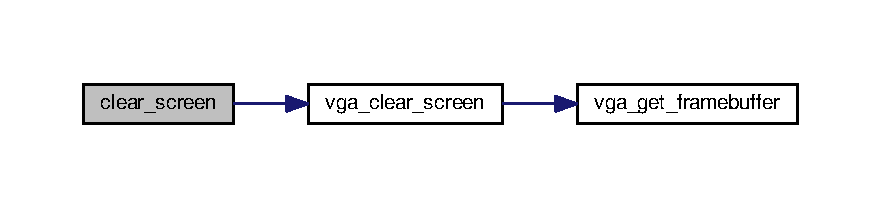
\includegraphics[width=350pt]{graphic_8h_abc40cd622f423abf44084c8f8595f57f_cgraph}
\end{center}
\end{figure}
\mbox{\Hypertarget{graphic_8h_a71625f77c43e97e5c5a8444877162556}\label{graphic_8h_a71625f77c43e97e5c5a8444877162556}} 
\index{graphic.\+h@{graphic.\+h}!console\+\_\+write\+\_\+keyboard@{console\+\_\+write\+\_\+keyboard}}
\index{console\+\_\+write\+\_\+keyboard@{console\+\_\+write\+\_\+keyboard}!graphic.\+h@{graphic.\+h}}
\subsubsection{\texorpdfstring{console\+\_\+write\+\_\+keyboard()}{console\_write\_keyboard()}}
{\footnotesize\ttfamily void console\+\_\+write\+\_\+keyboard (\begin{DoxyParamCaption}\item[{const char $\ast$}]{str,  }\item[{const \hyperlink{stdint_8h_a324c5d28c0d82f502a234ab99efac87a}{uint32\+\_\+t}}]{len }\end{DoxyParamCaption})}

Here is the call graph for this function\+:\nopagebreak
\begin{figure}[H]
\begin{center}
\leavevmode
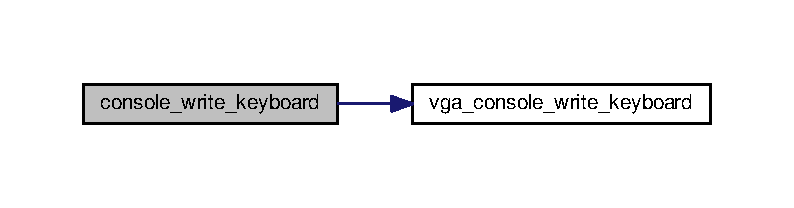
\includegraphics[width=350pt]{graphic_8h_a71625f77c43e97e5c5a8444877162556_cgraph}
\end{center}
\end{figure}
\mbox{\Hypertarget{graphic_8h_a839c7aea0eb4885f5270c20d95c6f224}\label{graphic_8h_a839c7aea0eb4885f5270c20d95c6f224}} 
\index{graphic.\+h@{graphic.\+h}!put\+\_\+cursor\+\_\+at@{put\+\_\+cursor\+\_\+at}}
\index{put\+\_\+cursor\+\_\+at@{put\+\_\+cursor\+\_\+at}!graphic.\+h@{graphic.\+h}}
\subsubsection{\texorpdfstring{put\+\_\+cursor\+\_\+at()}{put\_cursor\_at()}}
{\footnotesize\ttfamily \hyperlink{stddef_8h_a51557cb52bbb9ee9d55aab5b9b16c3d0}{O\+S\+\_\+\+R\+E\+T\+U\+R\+N\+\_\+E} put\+\_\+cursor\+\_\+at (\begin{DoxyParamCaption}\item[{const \hyperlink{stdint_8h_a324c5d28c0d82f502a234ab99efac87a}{uint32\+\_\+t}}]{line,  }\item[{const \hyperlink{stdint_8h_a324c5d28c0d82f502a234ab99efac87a}{uint32\+\_\+t}}]{column }\end{DoxyParamCaption})}

Here is the call graph for this function\+:\nopagebreak
\begin{figure}[H]
\begin{center}
\leavevmode
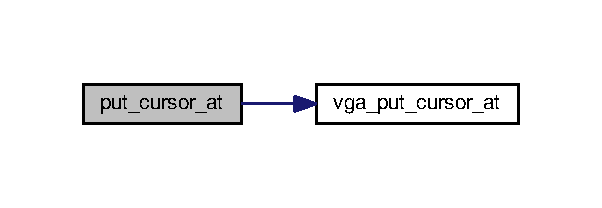
\includegraphics[width=289pt]{graphic_8h_a839c7aea0eb4885f5270c20d95c6f224_cgraph}
\end{center}
\end{figure}
\mbox{\Hypertarget{graphic_8h_a1e87d66055abaea40fde313f1446aa37}\label{graphic_8h_a1e87d66055abaea40fde313f1446aa37}} 
\index{graphic.\+h@{graphic.\+h}!restore\+\_\+cursor@{restore\+\_\+cursor}}
\index{restore\+\_\+cursor@{restore\+\_\+cursor}!graphic.\+h@{graphic.\+h}}
\subsubsection{\texorpdfstring{restore\+\_\+cursor()}{restore\_cursor()}}
{\footnotesize\ttfamily \hyperlink{stddef_8h_a51557cb52bbb9ee9d55aab5b9b16c3d0}{O\+S\+\_\+\+R\+E\+T\+U\+R\+N\+\_\+E} restore\+\_\+cursor (\begin{DoxyParamCaption}\item[{const \hyperlink{graphic_8h_a2377a22e1ea925fc95c5ec7b5bea95f5}{cursor\+\_\+t}}]{buffer }\end{DoxyParamCaption})}

Here is the call graph for this function\+:\nopagebreak
\begin{figure}[H]
\begin{center}
\leavevmode
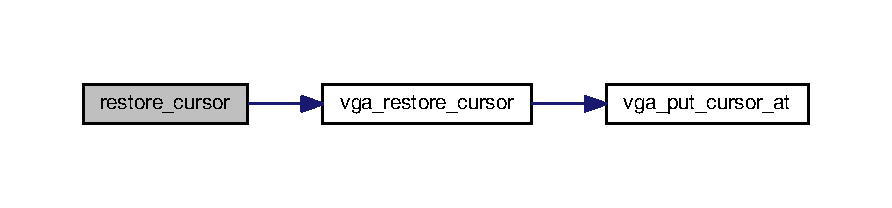
\includegraphics[width=350pt]{graphic_8h_a1e87d66055abaea40fde313f1446aa37_cgraph}
\end{center}
\end{figure}
\mbox{\Hypertarget{graphic_8h_a2233243d20d491dfcb4d9a5106ff53e6}\label{graphic_8h_a2233243d20d491dfcb4d9a5106ff53e6}} 
\index{graphic.\+h@{graphic.\+h}!save\+\_\+color\+\_\+scheme@{save\+\_\+color\+\_\+scheme}}
\index{save\+\_\+color\+\_\+scheme@{save\+\_\+color\+\_\+scheme}!graphic.\+h@{graphic.\+h}}
\subsubsection{\texorpdfstring{save\+\_\+color\+\_\+scheme()}{save\_color\_scheme()}}
{\footnotesize\ttfamily \hyperlink{stddef_8h_a51557cb52bbb9ee9d55aab5b9b16c3d0}{O\+S\+\_\+\+R\+E\+T\+U\+R\+N\+\_\+E} save\+\_\+color\+\_\+scheme (\begin{DoxyParamCaption}\item[{\hyperlink{graphic_8h_ad71288aca9a1e3d064316c1072f04bb7}{colorscheme\+\_\+t} $\ast$}]{buffer }\end{DoxyParamCaption})}

Here is the call graph for this function\+:\nopagebreak
\begin{figure}[H]
\begin{center}
\leavevmode
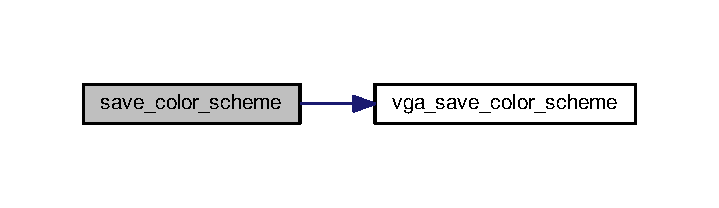
\includegraphics[width=345pt]{graphic_8h_a2233243d20d491dfcb4d9a5106ff53e6_cgraph}
\end{center}
\end{figure}
Here is the caller graph for this function\+:\nopagebreak
\begin{figure}[H]
\begin{center}
\leavevmode
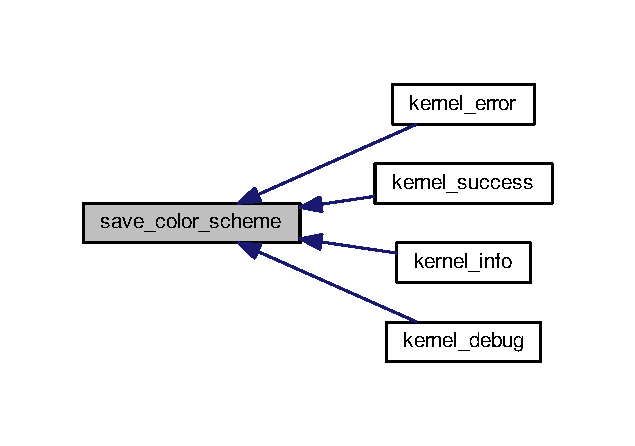
\includegraphics[width=305pt]{graphic_8h_a2233243d20d491dfcb4d9a5106ff53e6_icgraph}
\end{center}
\end{figure}
\mbox{\Hypertarget{graphic_8h_abc1ced411d18368a3d17840ca9fc5512}\label{graphic_8h_abc1ced411d18368a3d17840ca9fc5512}} 
\index{graphic.\+h@{graphic.\+h}!save\+\_\+cursor@{save\+\_\+cursor}}
\index{save\+\_\+cursor@{save\+\_\+cursor}!graphic.\+h@{graphic.\+h}}
\subsubsection{\texorpdfstring{save\+\_\+cursor()}{save\_cursor()}}
{\footnotesize\ttfamily \hyperlink{stddef_8h_a51557cb52bbb9ee9d55aab5b9b16c3d0}{O\+S\+\_\+\+R\+E\+T\+U\+R\+N\+\_\+E} save\+\_\+cursor (\begin{DoxyParamCaption}\item[{\hyperlink{graphic_8h_a2377a22e1ea925fc95c5ec7b5bea95f5}{cursor\+\_\+t} $\ast$}]{buffer }\end{DoxyParamCaption})}

Here is the call graph for this function\+:\nopagebreak
\begin{figure}[H]
\begin{center}
\leavevmode
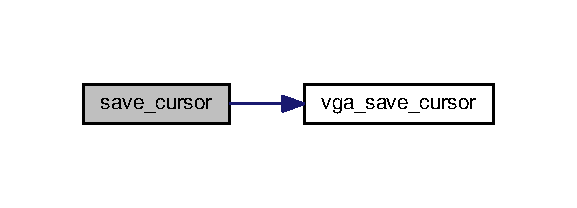
\includegraphics[width=277pt]{graphic_8h_abc1ced411d18368a3d17840ca9fc5512_cgraph}
\end{center}
\end{figure}
\mbox{\Hypertarget{graphic_8h_a38db267eb855286bed377c7dd921acb8}\label{graphic_8h_a38db267eb855286bed377c7dd921acb8}} 
\index{graphic.\+h@{graphic.\+h}!screen\+\_\+put\+\_\+char@{screen\+\_\+put\+\_\+char}}
\index{screen\+\_\+put\+\_\+char@{screen\+\_\+put\+\_\+char}!graphic.\+h@{graphic.\+h}}
\subsubsection{\texorpdfstring{screen\+\_\+put\+\_\+char()}{screen\_put\_char()}}
{\footnotesize\ttfamily void screen\+\_\+put\+\_\+char (\begin{DoxyParamCaption}\item[{const char}]{character }\end{DoxyParamCaption})}

Here is the caller graph for this function\+:\nopagebreak
\begin{figure}[H]
\begin{center}
\leavevmode
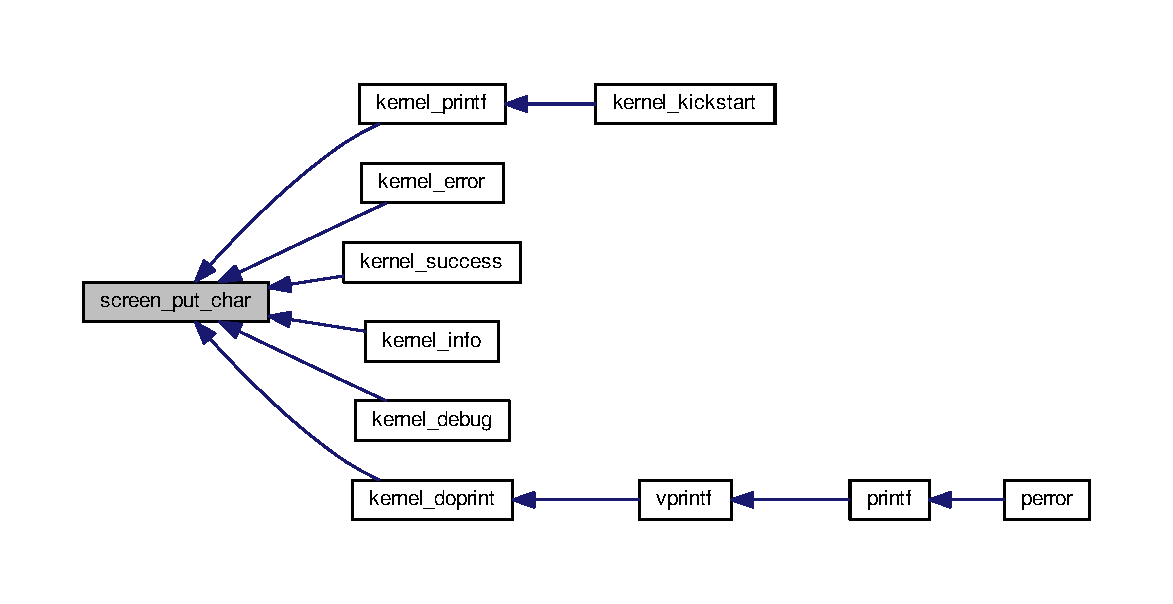
\includegraphics[width=350pt]{graphic_8h_a38db267eb855286bed377c7dd921acb8_icgraph}
\end{center}
\end{figure}
\mbox{\Hypertarget{graphic_8h_ad985618911547ca61e84432fe18e5b8c}\label{graphic_8h_ad985618911547ca61e84432fe18e5b8c}} 
\index{graphic.\+h@{graphic.\+h}!screen\+\_\+put\+\_\+string@{screen\+\_\+put\+\_\+string}}
\index{screen\+\_\+put\+\_\+string@{screen\+\_\+put\+\_\+string}!graphic.\+h@{graphic.\+h}}
\subsubsection{\texorpdfstring{screen\+\_\+put\+\_\+string()}{screen\_put\_string()}}
{\footnotesize\ttfamily void screen\+\_\+put\+\_\+string (\begin{DoxyParamCaption}\item[{const char $\ast$}]{str }\end{DoxyParamCaption})}

Here is the call graph for this function\+:\nopagebreak
\begin{figure}[H]
\begin{center}
\leavevmode
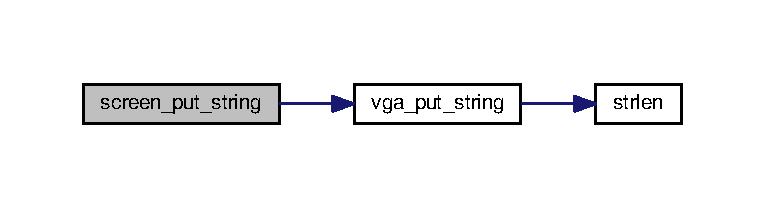
\includegraphics[width=350pt]{graphic_8h_ad985618911547ca61e84432fe18e5b8c_cgraph}
\end{center}
\end{figure}
Here is the caller graph for this function\+:\nopagebreak
\begin{figure}[H]
\begin{center}
\leavevmode
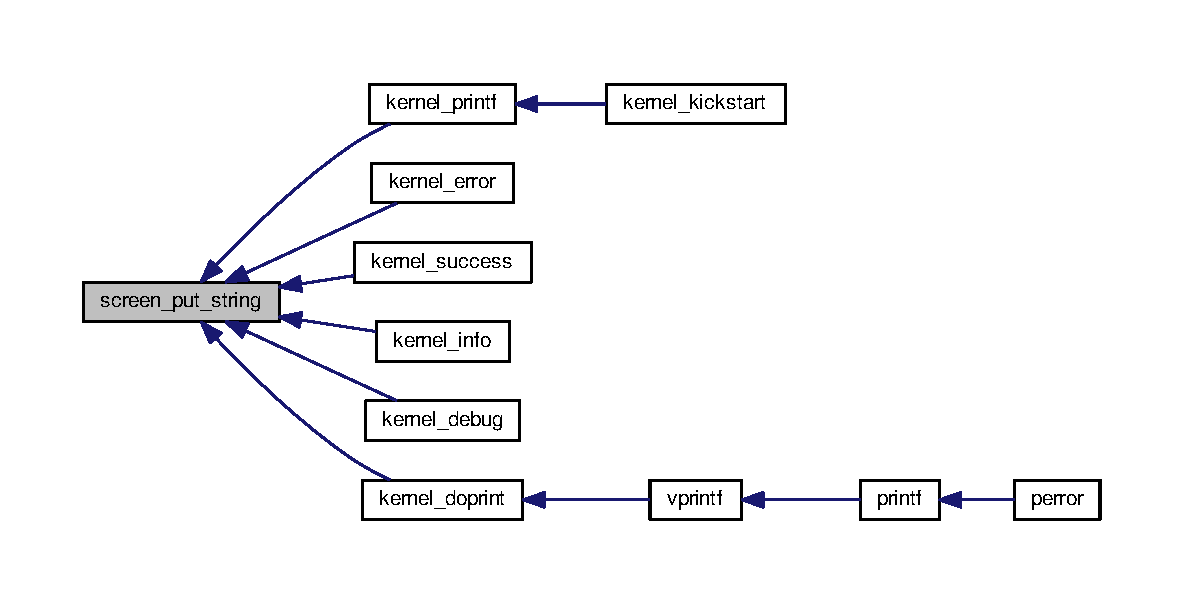
\includegraphics[width=350pt]{graphic_8h_ad985618911547ca61e84432fe18e5b8c_icgraph}
\end{center}
\end{figure}
\mbox{\Hypertarget{graphic_8h_a09a41c5d72f945277e7ce67b07a8dd79}\label{graphic_8h_a09a41c5d72f945277e7ce67b07a8dd79}} 
\index{graphic.\+h@{graphic.\+h}!scroll@{scroll}}
\index{scroll@{scroll}!graphic.\+h@{graphic.\+h}}
\subsubsection{\texorpdfstring{scroll()}{scroll()}}
{\footnotesize\ttfamily void scroll (\begin{DoxyParamCaption}\item[{const \hyperlink{graphic_8h_a223e9e8985b8d61206bd7628103b726f}{S\+C\+R\+O\+L\+L\+\_\+\+D\+I\+R\+E\+C\+T\+I\+O\+N\+\_\+E}}]{direction,  }\item[{const \hyperlink{stdint_8h_a324c5d28c0d82f502a234ab99efac87a}{uint32\+\_\+t}}]{lines\+\_\+count }\end{DoxyParamCaption})}

Here is the call graph for this function\+:\nopagebreak
\begin{figure}[H]
\begin{center}
\leavevmode
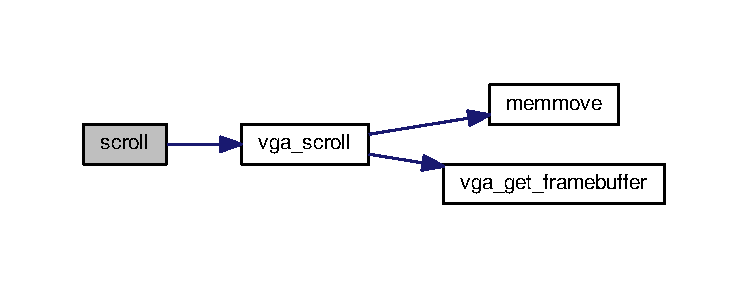
\includegraphics[width=350pt]{graphic_8h_a09a41c5d72f945277e7ce67b07a8dd79_cgraph}
\end{center}
\end{figure}
\mbox{\Hypertarget{graphic_8h_ab818d1480fd08b89d113e7951d139635}\label{graphic_8h_ab818d1480fd08b89d113e7951d139635}} 
\index{graphic.\+h@{graphic.\+h}!set\+\_\+color\+\_\+scheme@{set\+\_\+color\+\_\+scheme}}
\index{set\+\_\+color\+\_\+scheme@{set\+\_\+color\+\_\+scheme}!graphic.\+h@{graphic.\+h}}
\subsubsection{\texorpdfstring{set\+\_\+color\+\_\+scheme()}{set\_color\_scheme()}}
{\footnotesize\ttfamily void set\+\_\+color\+\_\+scheme (\begin{DoxyParamCaption}\item[{\hyperlink{graphic_8h_ad71288aca9a1e3d064316c1072f04bb7}{colorscheme\+\_\+t}}]{color\+\_\+scheme }\end{DoxyParamCaption})}

Here is the call graph for this function\+:\nopagebreak
\begin{figure}[H]
\begin{center}
\leavevmode
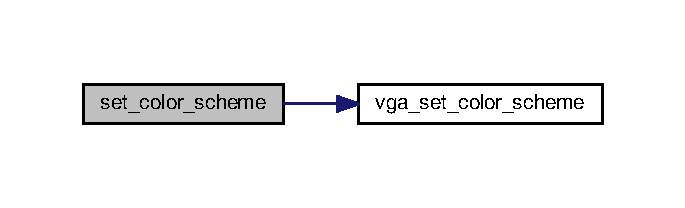
\includegraphics[width=329pt]{graphic_8h_ab818d1480fd08b89d113e7951d139635_cgraph}
\end{center}
\end{figure}
Here is the caller graph for this function\+:\nopagebreak
\begin{figure}[H]
\begin{center}
\leavevmode
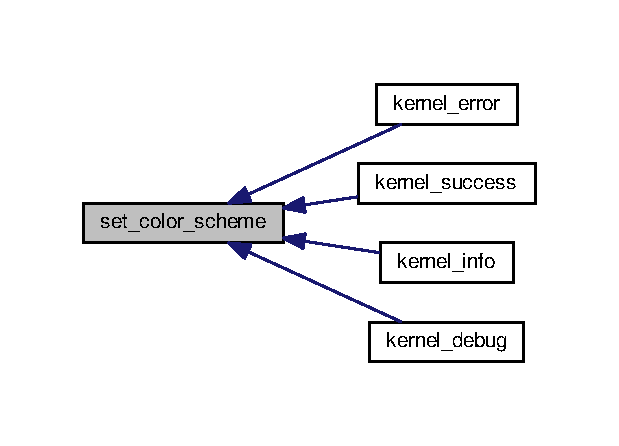
\includegraphics[width=297pt]{graphic_8h_ab818d1480fd08b89d113e7951d139635_icgraph}
\end{center}
\end{figure}
\mbox{\Hypertarget{graphic_8h_a456270cf61ec7c16f59eec8ce776b37f}\label{graphic_8h_a456270cf61ec7c16f59eec8ce776b37f}} 
\index{graphic.\+h@{graphic.\+h}!set\+\_\+selected\+\_\+driver@{set\+\_\+selected\+\_\+driver}}
\index{set\+\_\+selected\+\_\+driver@{set\+\_\+selected\+\_\+driver}!graphic.\+h@{graphic.\+h}}
\subsubsection{\texorpdfstring{set\+\_\+selected\+\_\+driver()}{set\_selected\_driver()}}
{\footnotesize\ttfamily void set\+\_\+selected\+\_\+driver (\begin{DoxyParamCaption}\item[{const \hyperlink{graphic_8h_a8731c83da869086e51c9576e7b24211b}{G\+R\+A\+P\+H\+I\+C\+\_\+\+D\+R\+I\+V\+E\+R\+\_\+E}}]{sel }\end{DoxyParamCaption})}


\hypertarget{serial_8h}{}\section{/home/alexy/\+Documents/\+Dev/\+R\+T\+L\+K\+I\+M/\+Source/\+Includes/\+Drivers/serial.h File Reference}
\label{serial_8h}\index{/home/alexy/\+Documents/\+Dev/\+R\+T\+L\+K\+I\+M/\+Source/\+Includes/\+Drivers/serial.\+h@{/home/alexy/\+Documents/\+Dev/\+R\+T\+L\+K\+I\+M/\+Source/\+Includes/\+Drivers/serial.\+h}}
{\ttfamily \#include $<$Lib/stdint.\+h$>$}\newline
{\ttfamily \#include $<$Lib/stddef.\+h$>$}\newline
Include dependency graph for serial.\+h\+:\nopagebreak
\begin{figure}[H]
\begin{center}
\leavevmode
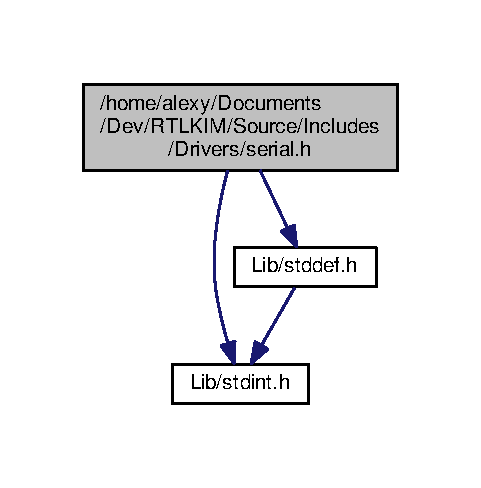
\includegraphics[width=231pt]{serial_8h__incl}
\end{center}
\end{figure}
This graph shows which files directly or indirectly include this file\+:\nopagebreak
\begin{figure}[H]
\begin{center}
\leavevmode
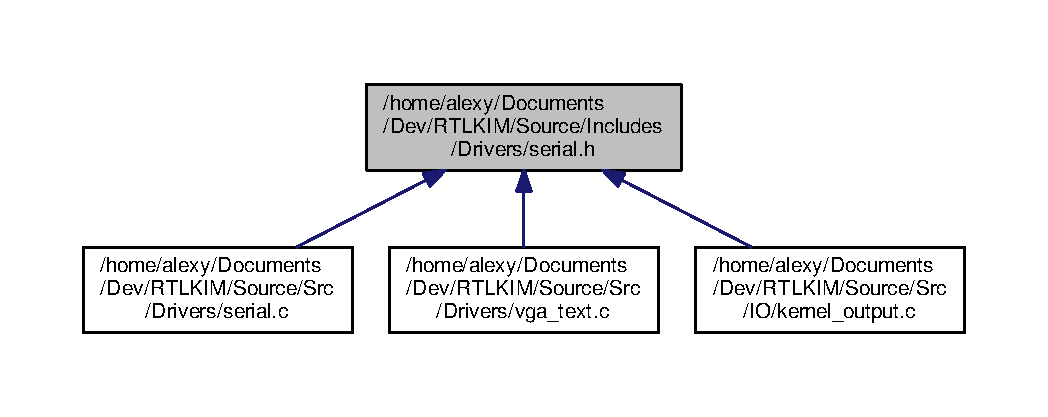
\includegraphics[width=350pt]{serial_8h__dep__incl}
\end{center}
\end{figure}
\subsection*{Macros}
\begin{DoxyCompactItemize}
\item 
\#define \hyperlink{serial_8h_a34365e17c472073dfba3681bb38054f3}{S\+E\+R\+I\+A\+L\+\_\+\+C\+O\+M1\+\_\+\+B\+A\+SE}~0x3\+F8
\item 
\#define \hyperlink{serial_8h_a1c2c6ce60cb9ef295cd0272b59196f82}{S\+E\+R\+I\+A\+L\+\_\+\+C\+O\+M2\+\_\+\+B\+A\+SE}~0x2\+F8
\item 
\#define \hyperlink{serial_8h_aa468a88b2acccde9bbf5e401f5d88eaf}{S\+E\+R\+I\+A\+L\+\_\+\+C\+O\+M3\+\_\+\+B\+A\+SE}~0x3\+E8
\item 
\#define \hyperlink{serial_8h_acebbaec5ade4a12ee12ff0587a86ed94}{S\+E\+R\+I\+A\+L\+\_\+\+C\+O\+M4\+\_\+\+B\+A\+SE}~0x2\+E8
\item 
\#define \hyperlink{serial_8h_a00dbb3ab1c59e14699be9393693e2248}{C\+O\+M1}~\hyperlink{serial_8h_a34365e17c472073dfba3681bb38054f3}{S\+E\+R\+I\+A\+L\+\_\+\+C\+O\+M1\+\_\+\+B\+A\+SE}
\item 
\#define \hyperlink{serial_8h_a435e02f194c24c9b0e00d7cd27a1704e}{C\+O\+M2}~\hyperlink{serial_8h_a1c2c6ce60cb9ef295cd0272b59196f82}{S\+E\+R\+I\+A\+L\+\_\+\+C\+O\+M2\+\_\+\+B\+A\+SE}
\item 
\#define \hyperlink{serial_8h_abbed02672431595364c5dd35809303a6}{C\+O\+M3}~\hyperlink{serial_8h_aa468a88b2acccde9bbf5e401f5d88eaf}{S\+E\+R\+I\+A\+L\+\_\+\+C\+O\+M3\+\_\+\+B\+A\+SE}
\item 
\#define \hyperlink{serial_8h_a595cabb01568ba641574d24546d99c6b}{C\+O\+M4}~\hyperlink{serial_8h_acebbaec5ade4a12ee12ff0587a86ed94}{S\+E\+R\+I\+A\+L\+\_\+\+C\+O\+M4\+\_\+\+B\+A\+SE}
\item 
\#define \hyperlink{serial_8h_a6ceb96bbfa52d1c529bd657b698d5a40}{S\+E\+R\+I\+A\+L\+\_\+\+D\+E\+B\+U\+G\+\_\+\+P\+O\+RT}~\hyperlink{serial_8h_a00dbb3ab1c59e14699be9393693e2248}{C\+O\+M1}
\item 
\#define \hyperlink{serial_8h_a8351903aa481452402cad5df0a8aa26b}{S\+E\+R\+I\+A\+L\+\_\+\+D\+A\+T\+A\+\_\+\+P\+O\+RT}(port)~(port)
\item 
\#define \hyperlink{serial_8h_a8d60baa849072d23cd603ae759305324}{S\+E\+R\+I\+A\+L\+\_\+\+D\+A\+T\+A\+\_\+\+P\+O\+R\+T\+\_\+2}(port)~(port + 1)
\item 
\#define \hyperlink{serial_8h_a5ec9e2db08925548507011ff925b9144}{S\+E\+R\+I\+A\+L\+\_\+\+F\+I\+F\+O\+\_\+\+C\+O\+M\+M\+A\+N\+D\+\_\+\+P\+O\+RT}(port)~(port + 2)
\item 
\#define \hyperlink{serial_8h_a2c43926d233806ee5e61a65d918db34d}{S\+E\+R\+I\+A\+L\+\_\+\+L\+I\+N\+E\+\_\+\+C\+O\+M\+M\+A\+N\+D\+\_\+\+P\+O\+RT}(port)~(port + 3)
\item 
\#define \hyperlink{serial_8h_a0945f52a518604a02f87e33a10a59df7}{S\+E\+R\+I\+A\+L\+\_\+\+M\+O\+D\+E\+M\+\_\+\+C\+O\+M\+M\+A\+N\+D\+\_\+\+P\+O\+RT}(port)~(port + 4)
\item 
\#define \hyperlink{serial_8h_af50c4f78311a57efbc1cfa3c694b1e77}{S\+E\+R\+I\+A\+L\+\_\+\+L\+I\+N\+E\+\_\+\+S\+T\+A\+T\+U\+S\+\_\+\+P\+O\+RT}(port)~(port + 5)
\item 
\#define \hyperlink{serial_8h_a4bd0c20da37480ffee47598349e9e0fe}{S\+E\+R\+I\+A\+L\+\_\+\+D\+A\+T\+A\+\_\+\+L\+E\+N\+G\+T\+H\+\_\+5}~0x00
\item 
\#define \hyperlink{serial_8h_ad4edc01bd90ce73ee711cd3919428b22}{S\+E\+R\+I\+A\+L\+\_\+\+D\+A\+T\+A\+\_\+\+L\+E\+N\+G\+T\+H\+\_\+6}~0x01
\item 
\#define \hyperlink{serial_8h_a34e3930664271c4bda7b9eb1675b9cd0}{S\+E\+R\+I\+A\+L\+\_\+\+D\+A\+T\+A\+\_\+\+L\+E\+N\+G\+T\+H\+\_\+7}~0x02
\item 
\#define \hyperlink{serial_8h_ab7d8c6b3660b431109c909755e457c26}{S\+E\+R\+I\+A\+L\+\_\+\+D\+A\+T\+A\+\_\+\+L\+E\+N\+G\+T\+H\+\_\+8}~0x03
\item 
\#define \hyperlink{serial_8h_a1e1822ba21f5e720c09e1712576413f4}{S\+E\+R\+I\+A\+L\+\_\+\+S\+T\+O\+P\+\_\+\+B\+I\+T\+\_\+1}~0x00
\item 
\#define \hyperlink{serial_8h_ac743d7fbebfa22ae199ae7885afea07c}{S\+E\+R\+I\+A\+L\+\_\+\+S\+T\+O\+P\+\_\+\+B\+I\+T\+\_\+2}~0x04
\item 
\#define \hyperlink{serial_8h_ad3af92391cfd2670eb782a60c7f923a6}{S\+E\+R\+I\+A\+L\+\_\+\+P\+A\+R\+I\+T\+Y\+\_\+\+N\+O\+NE}~0x00
\item 
\#define \hyperlink{serial_8h_aa1baeda93fe64b888113824d02471d0f}{S\+E\+R\+I\+A\+L\+\_\+\+P\+A\+R\+I\+T\+Y\+\_\+\+O\+DD}~0x01
\item 
\#define \hyperlink{serial_8h_ab1469484b1ad5e39561c21b5a590eaf6}{S\+E\+R\+I\+A\+L\+\_\+\+P\+A\+R\+I\+T\+Y\+\_\+\+E\+V\+EN}~0x03
\item 
\#define \hyperlink{serial_8h_a4b3897d63a1a6d5ced0feff0d3ce3460}{S\+E\+R\+I\+A\+L\+\_\+\+P\+A\+R\+I\+T\+Y\+\_\+\+M\+A\+RK}~0x05
\item 
\#define \hyperlink{serial_8h_ad5ab869b9c6d8c3dfaefe9c913d55ce7}{S\+E\+R\+I\+A\+L\+\_\+\+P\+A\+R\+I\+T\+Y\+\_\+\+S\+P\+A\+CE}~0x07
\item 
\#define \hyperlink{serial_8h_a8f5a71c87dac509b1ef7e52c3c56cf98}{S\+E\+R\+I\+A\+L\+\_\+\+B\+R\+E\+A\+K\+\_\+\+C\+T\+R\+L\+\_\+\+E\+N\+A\+B\+L\+ED}~0x40
\item 
\#define \hyperlink{serial_8h_afb9ca3f7eecfdcf16088b917d2d8003a}{S\+E\+R\+I\+A\+L\+\_\+\+B\+R\+E\+A\+K\+\_\+\+C\+T\+R\+L\+\_\+\+D\+I\+S\+A\+B\+L\+ED}~0x00
\item 
\#define \hyperlink{serial_8h_a873382b43e1973a22b6ce75f02c6a182}{S\+E\+R\+I\+A\+L\+\_\+\+D\+L\+A\+B\+\_\+\+E\+N\+A\+B\+L\+ED}~0x80
\item 
\#define \hyperlink{serial_8h_af3725655502b7f6f733daed938982c41}{S\+E\+R\+I\+A\+L\+\_\+\+D\+L\+A\+B\+\_\+\+D\+I\+S\+A\+B\+L\+ED}~0x00
\item 
\#define \hyperlink{serial_8h_ac9e29bed47741802d3a895b7d43e3962}{S\+E\+R\+I\+A\+L\+\_\+\+E\+N\+A\+B\+L\+E\+\_\+\+F\+I\+FO}~0x01
\item 
\#define \hyperlink{serial_8h_a2a60628f88ee6bc4c4259f29a0bd770d}{S\+E\+R\+I\+A\+L\+\_\+\+C\+L\+E\+A\+R\+\_\+\+R\+E\+C\+V\+\_\+\+F\+I\+FO}~0x02
\item 
\#define \hyperlink{serial_8h_af80ebedb3b15dbd522485b6b69530721}{S\+E\+R\+I\+A\+L\+\_\+\+C\+L\+E\+A\+R\+\_\+\+S\+E\+N\+D\+\_\+\+F\+I\+FO}~0x04
\item 
\#define \hyperlink{serial_8h_a73de4996e9764e8c5d2db9e20132d34d}{S\+E\+R\+I\+A\+L\+\_\+\+D\+M\+A\+\_\+\+A\+C\+C\+E\+S\+S\+E\+D\+\_\+\+F\+I\+FO}~0x08
\item 
\#define \hyperlink{serial_8h_a7018e1e74723032a45448e320dd89936}{S\+E\+R\+I\+A\+L\+\_\+\+F\+I\+F\+O\+\_\+\+D\+E\+P\+T\+H\+\_\+14}~0x00
\item 
\#define \hyperlink{serial_8h_a4dde9b9b638a98af4035c66bfb5dfebc}{S\+E\+R\+I\+A\+L\+\_\+\+F\+I\+F\+O\+\_\+\+D\+E\+P\+T\+H\+\_\+64}~0x10
\end{DoxyCompactItemize}
\subsection*{Typedefs}
\begin{DoxyCompactItemize}
\item 
typedef enum \hyperlink{serial_8h_ab2f4dc67da7fe04c5c51e6dcd6514447}{S\+E\+R\+I\+A\+L\+\_\+\+B\+A\+U\+D\+R\+A\+TE} \hyperlink{serial_8h_aca832d7d7778d54533f0ff03c12f343e}{S\+E\+R\+I\+A\+L\+\_\+\+B\+A\+U\+D\+R\+A\+T\+E\+\_\+E}
\end{DoxyCompactItemize}
\subsection*{Enumerations}
\begin{DoxyCompactItemize}
\item 
enum \hyperlink{serial_8h_ab2f4dc67da7fe04c5c51e6dcd6514447}{S\+E\+R\+I\+A\+L\+\_\+\+B\+A\+U\+D\+R\+A\+TE} \{ \newline
\hyperlink{serial_8h_ab2f4dc67da7fe04c5c51e6dcd6514447a649a1229bb2eb57d0be8a80fe824aae9}{B\+A\+U\+R\+D\+A\+T\+E\+\_\+50} = 2304, 
\hyperlink{serial_8h_ab2f4dc67da7fe04c5c51e6dcd6514447a0d159d9a1aa934e978497e70fc598160}{B\+A\+U\+D\+R\+A\+T\+E\+\_\+75} = 1536, 
\hyperlink{serial_8h_ab2f4dc67da7fe04c5c51e6dcd6514447aad67725e89462654dd5f687cdd776092}{B\+A\+U\+D\+R\+A\+T\+E\+\_\+150} = 768, 
\hyperlink{serial_8h_ab2f4dc67da7fe04c5c51e6dcd6514447a1dfed302a249d5d472d9a39aa11afdcd}{B\+A\+U\+D\+R\+A\+T\+E\+\_\+300} = 384, 
\newline
\hyperlink{serial_8h_ab2f4dc67da7fe04c5c51e6dcd6514447a32ec63c5760f2d9ddc1d90c1d3d84f75}{B\+A\+U\+D\+R\+A\+T\+E\+\_\+600} = 192, 
\hyperlink{serial_8h_ab2f4dc67da7fe04c5c51e6dcd6514447ac3b902a0c54578ee8e732d61ca330415}{B\+A\+U\+D\+R\+A\+T\+E\+\_\+1200} = 96, 
\hyperlink{serial_8h_ab2f4dc67da7fe04c5c51e6dcd6514447ad7bdd6696316e62c77c3edd447cf5854}{B\+A\+U\+D\+R\+A\+T\+E\+\_\+1800} = 64, 
\hyperlink{serial_8h_ab2f4dc67da7fe04c5c51e6dcd6514447af75b6bf10bafe82b79c9afd065eb48d9}{B\+A\+U\+D\+R\+A\+T\+E\+\_\+2400} = 48, 
\newline
\hyperlink{serial_8h_ab2f4dc67da7fe04c5c51e6dcd6514447abeff4d0442f2d2e14dcfaf6cc28306af}{B\+A\+U\+D\+R\+A\+T\+E\+\_\+4800} = 24, 
\hyperlink{serial_8h_ab2f4dc67da7fe04c5c51e6dcd6514447a33a90321f934176874fce95787023c77}{B\+A\+U\+D\+R\+A\+T\+E\+\_\+7200} = 16, 
\hyperlink{serial_8h_ab2f4dc67da7fe04c5c51e6dcd6514447a269fd588c1f05f78ec00345ee464690c}{B\+A\+U\+D\+R\+A\+T\+E\+\_\+9600} = 12, 
\hyperlink{serial_8h_ab2f4dc67da7fe04c5c51e6dcd6514447ad7b08eb1b83834871da8caed89634914}{B\+A\+U\+D\+R\+A\+T\+E\+\_\+14400} = 8, 
\newline
\hyperlink{serial_8h_ab2f4dc67da7fe04c5c51e6dcd6514447a0a793a8d7b4c0c7b3667a20750ba6dcd}{B\+A\+U\+D\+R\+A\+T\+E\+\_\+19200} = 6, 
\hyperlink{serial_8h_ab2f4dc67da7fe04c5c51e6dcd6514447ab6992595f5799026f56f62688d3d928b}{B\+A\+U\+D\+R\+A\+T\+E\+\_\+38400} = 3, 
\hyperlink{serial_8h_ab2f4dc67da7fe04c5c51e6dcd6514447a9f210b73ceb88265b53e278af7c62ee9}{B\+A\+U\+D\+R\+A\+T\+E\+\_\+57600} = 2, 
\hyperlink{serial_8h_ab2f4dc67da7fe04c5c51e6dcd6514447a6e697dd0f979fbfd5ab8e8fc9518a5c8}{B\+A\+U\+D\+R\+A\+T\+E\+\_\+115200} = 1
 \}
\end{DoxyCompactItemize}
\subsection*{Functions}
\begin{DoxyCompactItemize}
\item 
\hyperlink{stddef_8h_a51557cb52bbb9ee9d55aab5b9b16c3d0}{O\+S\+\_\+\+R\+E\+T\+U\+R\+N\+\_\+E} \hyperlink{serial_8h_a127638fb58a6cf0f0f880ae1697e2c33}{init\+\_\+serial} (void)
\item 
\hyperlink{stddef_8h_a51557cb52bbb9ee9d55aab5b9b16c3d0}{O\+S\+\_\+\+R\+E\+T\+U\+R\+N\+\_\+E} \hyperlink{serial_8h_a7f495d0c087113f47373769976d852f9}{init\+\_\+serial\+\_\+interrupt} (void)
\item 
void \hyperlink{serial_8h_afb7bd137c3cca6f25fb34170ff58c999}{serial\+\_\+write} (const \hyperlink{stdint_8h_a324c5d28c0d82f502a234ab99efac87a}{uint32\+\_\+t} port, const \hyperlink{stdint_8h_aba7bc1797add20fe3efdf37ced1182c5}{uint8\+\_\+t} data)
\item 
void \hyperlink{serial_8h_a89ce044b86475f9d3e3688b7cb043cc8}{serial\+\_\+put\+\_\+string} (const char $\ast$string)
\item 
void \hyperlink{serial_8h_a94affa1c8d77a69875f10c4915614afe}{serial\+\_\+put\+\_\+char} (const char character)
\item 
\hyperlink{stdint_8h_aba7bc1797add20fe3efdf37ced1182c5}{uint8\+\_\+t} \hyperlink{serial_8h_a45e1160c98d53c1306e75a32d54e81a3}{serial\+\_\+received} (const \hyperlink{stdint_8h_a324c5d28c0d82f502a234ab99efac87a}{uint32\+\_\+t} port)
\item 
\hyperlink{stdint_8h_aba7bc1797add20fe3efdf37ced1182c5}{uint8\+\_\+t} \hyperlink{serial_8h_ab3b28cf37d70288fb56ad06c1815d824}{read\+\_\+serial} (const \hyperlink{stdint_8h_a324c5d28c0d82f502a234ab99efac87a}{uint32\+\_\+t} port)
\end{DoxyCompactItemize}


\subsection{Macro Definition Documentation}
\mbox{\Hypertarget{serial_8h_a00dbb3ab1c59e14699be9393693e2248}\label{serial_8h_a00dbb3ab1c59e14699be9393693e2248}} 
\index{serial.\+h@{serial.\+h}!C\+O\+M1@{C\+O\+M1}}
\index{C\+O\+M1@{C\+O\+M1}!serial.\+h@{serial.\+h}}
\subsubsection{\texorpdfstring{C\+O\+M1}{COM1}}
{\footnotesize\ttfamily \#define C\+O\+M1~\hyperlink{serial_8h_a34365e17c472073dfba3681bb38054f3}{S\+E\+R\+I\+A\+L\+\_\+\+C\+O\+M1\+\_\+\+B\+A\+SE}}

\mbox{\Hypertarget{serial_8h_a435e02f194c24c9b0e00d7cd27a1704e}\label{serial_8h_a435e02f194c24c9b0e00d7cd27a1704e}} 
\index{serial.\+h@{serial.\+h}!C\+O\+M2@{C\+O\+M2}}
\index{C\+O\+M2@{C\+O\+M2}!serial.\+h@{serial.\+h}}
\subsubsection{\texorpdfstring{C\+O\+M2}{COM2}}
{\footnotesize\ttfamily \#define C\+O\+M2~\hyperlink{serial_8h_a1c2c6ce60cb9ef295cd0272b59196f82}{S\+E\+R\+I\+A\+L\+\_\+\+C\+O\+M2\+\_\+\+B\+A\+SE}}

\mbox{\Hypertarget{serial_8h_abbed02672431595364c5dd35809303a6}\label{serial_8h_abbed02672431595364c5dd35809303a6}} 
\index{serial.\+h@{serial.\+h}!C\+O\+M3@{C\+O\+M3}}
\index{C\+O\+M3@{C\+O\+M3}!serial.\+h@{serial.\+h}}
\subsubsection{\texorpdfstring{C\+O\+M3}{COM3}}
{\footnotesize\ttfamily \#define C\+O\+M3~\hyperlink{serial_8h_aa468a88b2acccde9bbf5e401f5d88eaf}{S\+E\+R\+I\+A\+L\+\_\+\+C\+O\+M3\+\_\+\+B\+A\+SE}}

\mbox{\Hypertarget{serial_8h_a595cabb01568ba641574d24546d99c6b}\label{serial_8h_a595cabb01568ba641574d24546d99c6b}} 
\index{serial.\+h@{serial.\+h}!C\+O\+M4@{C\+O\+M4}}
\index{C\+O\+M4@{C\+O\+M4}!serial.\+h@{serial.\+h}}
\subsubsection{\texorpdfstring{C\+O\+M4}{COM4}}
{\footnotesize\ttfamily \#define C\+O\+M4~\hyperlink{serial_8h_acebbaec5ade4a12ee12ff0587a86ed94}{S\+E\+R\+I\+A\+L\+\_\+\+C\+O\+M4\+\_\+\+B\+A\+SE}}

\mbox{\Hypertarget{serial_8h_afb9ca3f7eecfdcf16088b917d2d8003a}\label{serial_8h_afb9ca3f7eecfdcf16088b917d2d8003a}} 
\index{serial.\+h@{serial.\+h}!S\+E\+R\+I\+A\+L\+\_\+\+B\+R\+E\+A\+K\+\_\+\+C\+T\+R\+L\+\_\+\+D\+I\+S\+A\+B\+L\+ED@{S\+E\+R\+I\+A\+L\+\_\+\+B\+R\+E\+A\+K\+\_\+\+C\+T\+R\+L\+\_\+\+D\+I\+S\+A\+B\+L\+ED}}
\index{S\+E\+R\+I\+A\+L\+\_\+\+B\+R\+E\+A\+K\+\_\+\+C\+T\+R\+L\+\_\+\+D\+I\+S\+A\+B\+L\+ED@{S\+E\+R\+I\+A\+L\+\_\+\+B\+R\+E\+A\+K\+\_\+\+C\+T\+R\+L\+\_\+\+D\+I\+S\+A\+B\+L\+ED}!serial.\+h@{serial.\+h}}
\subsubsection{\texorpdfstring{S\+E\+R\+I\+A\+L\+\_\+\+B\+R\+E\+A\+K\+\_\+\+C\+T\+R\+L\+\_\+\+D\+I\+S\+A\+B\+L\+ED}{SERIAL\_BREAK\_CTRL\_DISABLED}}
{\footnotesize\ttfamily \#define S\+E\+R\+I\+A\+L\+\_\+\+B\+R\+E\+A\+K\+\_\+\+C\+T\+R\+L\+\_\+\+D\+I\+S\+A\+B\+L\+ED~0x00}

\mbox{\Hypertarget{serial_8h_a8f5a71c87dac509b1ef7e52c3c56cf98}\label{serial_8h_a8f5a71c87dac509b1ef7e52c3c56cf98}} 
\index{serial.\+h@{serial.\+h}!S\+E\+R\+I\+A\+L\+\_\+\+B\+R\+E\+A\+K\+\_\+\+C\+T\+R\+L\+\_\+\+E\+N\+A\+B\+L\+ED@{S\+E\+R\+I\+A\+L\+\_\+\+B\+R\+E\+A\+K\+\_\+\+C\+T\+R\+L\+\_\+\+E\+N\+A\+B\+L\+ED}}
\index{S\+E\+R\+I\+A\+L\+\_\+\+B\+R\+E\+A\+K\+\_\+\+C\+T\+R\+L\+\_\+\+E\+N\+A\+B\+L\+ED@{S\+E\+R\+I\+A\+L\+\_\+\+B\+R\+E\+A\+K\+\_\+\+C\+T\+R\+L\+\_\+\+E\+N\+A\+B\+L\+ED}!serial.\+h@{serial.\+h}}
\subsubsection{\texorpdfstring{S\+E\+R\+I\+A\+L\+\_\+\+B\+R\+E\+A\+K\+\_\+\+C\+T\+R\+L\+\_\+\+E\+N\+A\+B\+L\+ED}{SERIAL\_BREAK\_CTRL\_ENABLED}}
{\footnotesize\ttfamily \#define S\+E\+R\+I\+A\+L\+\_\+\+B\+R\+E\+A\+K\+\_\+\+C\+T\+R\+L\+\_\+\+E\+N\+A\+B\+L\+ED~0x40}

\mbox{\Hypertarget{serial_8h_a2a60628f88ee6bc4c4259f29a0bd770d}\label{serial_8h_a2a60628f88ee6bc4c4259f29a0bd770d}} 
\index{serial.\+h@{serial.\+h}!S\+E\+R\+I\+A\+L\+\_\+\+C\+L\+E\+A\+R\+\_\+\+R\+E\+C\+V\+\_\+\+F\+I\+FO@{S\+E\+R\+I\+A\+L\+\_\+\+C\+L\+E\+A\+R\+\_\+\+R\+E\+C\+V\+\_\+\+F\+I\+FO}}
\index{S\+E\+R\+I\+A\+L\+\_\+\+C\+L\+E\+A\+R\+\_\+\+R\+E\+C\+V\+\_\+\+F\+I\+FO@{S\+E\+R\+I\+A\+L\+\_\+\+C\+L\+E\+A\+R\+\_\+\+R\+E\+C\+V\+\_\+\+F\+I\+FO}!serial.\+h@{serial.\+h}}
\subsubsection{\texorpdfstring{S\+E\+R\+I\+A\+L\+\_\+\+C\+L\+E\+A\+R\+\_\+\+R\+E\+C\+V\+\_\+\+F\+I\+FO}{SERIAL\_CLEAR\_RECV\_FIFO}}
{\footnotesize\ttfamily \#define S\+E\+R\+I\+A\+L\+\_\+\+C\+L\+E\+A\+R\+\_\+\+R\+E\+C\+V\+\_\+\+F\+I\+FO~0x02}

\mbox{\Hypertarget{serial_8h_af80ebedb3b15dbd522485b6b69530721}\label{serial_8h_af80ebedb3b15dbd522485b6b69530721}} 
\index{serial.\+h@{serial.\+h}!S\+E\+R\+I\+A\+L\+\_\+\+C\+L\+E\+A\+R\+\_\+\+S\+E\+N\+D\+\_\+\+F\+I\+FO@{S\+E\+R\+I\+A\+L\+\_\+\+C\+L\+E\+A\+R\+\_\+\+S\+E\+N\+D\+\_\+\+F\+I\+FO}}
\index{S\+E\+R\+I\+A\+L\+\_\+\+C\+L\+E\+A\+R\+\_\+\+S\+E\+N\+D\+\_\+\+F\+I\+FO@{S\+E\+R\+I\+A\+L\+\_\+\+C\+L\+E\+A\+R\+\_\+\+S\+E\+N\+D\+\_\+\+F\+I\+FO}!serial.\+h@{serial.\+h}}
\subsubsection{\texorpdfstring{S\+E\+R\+I\+A\+L\+\_\+\+C\+L\+E\+A\+R\+\_\+\+S\+E\+N\+D\+\_\+\+F\+I\+FO}{SERIAL\_CLEAR\_SEND\_FIFO}}
{\footnotesize\ttfamily \#define S\+E\+R\+I\+A\+L\+\_\+\+C\+L\+E\+A\+R\+\_\+\+S\+E\+N\+D\+\_\+\+F\+I\+FO~0x04}

\mbox{\Hypertarget{serial_8h_a34365e17c472073dfba3681bb38054f3}\label{serial_8h_a34365e17c472073dfba3681bb38054f3}} 
\index{serial.\+h@{serial.\+h}!S\+E\+R\+I\+A\+L\+\_\+\+C\+O\+M1\+\_\+\+B\+A\+SE@{S\+E\+R\+I\+A\+L\+\_\+\+C\+O\+M1\+\_\+\+B\+A\+SE}}
\index{S\+E\+R\+I\+A\+L\+\_\+\+C\+O\+M1\+\_\+\+B\+A\+SE@{S\+E\+R\+I\+A\+L\+\_\+\+C\+O\+M1\+\_\+\+B\+A\+SE}!serial.\+h@{serial.\+h}}
\subsubsection{\texorpdfstring{S\+E\+R\+I\+A\+L\+\_\+\+C\+O\+M1\+\_\+\+B\+A\+SE}{SERIAL\_COM1\_BASE}}
{\footnotesize\ttfamily \#define S\+E\+R\+I\+A\+L\+\_\+\+C\+O\+M1\+\_\+\+B\+A\+SE~0x3\+F8}

\mbox{\Hypertarget{serial_8h_a1c2c6ce60cb9ef295cd0272b59196f82}\label{serial_8h_a1c2c6ce60cb9ef295cd0272b59196f82}} 
\index{serial.\+h@{serial.\+h}!S\+E\+R\+I\+A\+L\+\_\+\+C\+O\+M2\+\_\+\+B\+A\+SE@{S\+E\+R\+I\+A\+L\+\_\+\+C\+O\+M2\+\_\+\+B\+A\+SE}}
\index{S\+E\+R\+I\+A\+L\+\_\+\+C\+O\+M2\+\_\+\+B\+A\+SE@{S\+E\+R\+I\+A\+L\+\_\+\+C\+O\+M2\+\_\+\+B\+A\+SE}!serial.\+h@{serial.\+h}}
\subsubsection{\texorpdfstring{S\+E\+R\+I\+A\+L\+\_\+\+C\+O\+M2\+\_\+\+B\+A\+SE}{SERIAL\_COM2\_BASE}}
{\footnotesize\ttfamily \#define S\+E\+R\+I\+A\+L\+\_\+\+C\+O\+M2\+\_\+\+B\+A\+SE~0x2\+F8}

\mbox{\Hypertarget{serial_8h_aa468a88b2acccde9bbf5e401f5d88eaf}\label{serial_8h_aa468a88b2acccde9bbf5e401f5d88eaf}} 
\index{serial.\+h@{serial.\+h}!S\+E\+R\+I\+A\+L\+\_\+\+C\+O\+M3\+\_\+\+B\+A\+SE@{S\+E\+R\+I\+A\+L\+\_\+\+C\+O\+M3\+\_\+\+B\+A\+SE}}
\index{S\+E\+R\+I\+A\+L\+\_\+\+C\+O\+M3\+\_\+\+B\+A\+SE@{S\+E\+R\+I\+A\+L\+\_\+\+C\+O\+M3\+\_\+\+B\+A\+SE}!serial.\+h@{serial.\+h}}
\subsubsection{\texorpdfstring{S\+E\+R\+I\+A\+L\+\_\+\+C\+O\+M3\+\_\+\+B\+A\+SE}{SERIAL\_COM3\_BASE}}
{\footnotesize\ttfamily \#define S\+E\+R\+I\+A\+L\+\_\+\+C\+O\+M3\+\_\+\+B\+A\+SE~0x3\+E8}

\mbox{\Hypertarget{serial_8h_acebbaec5ade4a12ee12ff0587a86ed94}\label{serial_8h_acebbaec5ade4a12ee12ff0587a86ed94}} 
\index{serial.\+h@{serial.\+h}!S\+E\+R\+I\+A\+L\+\_\+\+C\+O\+M4\+\_\+\+B\+A\+SE@{S\+E\+R\+I\+A\+L\+\_\+\+C\+O\+M4\+\_\+\+B\+A\+SE}}
\index{S\+E\+R\+I\+A\+L\+\_\+\+C\+O\+M4\+\_\+\+B\+A\+SE@{S\+E\+R\+I\+A\+L\+\_\+\+C\+O\+M4\+\_\+\+B\+A\+SE}!serial.\+h@{serial.\+h}}
\subsubsection{\texorpdfstring{S\+E\+R\+I\+A\+L\+\_\+\+C\+O\+M4\+\_\+\+B\+A\+SE}{SERIAL\_COM4\_BASE}}
{\footnotesize\ttfamily \#define S\+E\+R\+I\+A\+L\+\_\+\+C\+O\+M4\+\_\+\+B\+A\+SE~0x2\+E8}

\mbox{\Hypertarget{serial_8h_a4bd0c20da37480ffee47598349e9e0fe}\label{serial_8h_a4bd0c20da37480ffee47598349e9e0fe}} 
\index{serial.\+h@{serial.\+h}!S\+E\+R\+I\+A\+L\+\_\+\+D\+A\+T\+A\+\_\+\+L\+E\+N\+G\+T\+H\+\_\+5@{S\+E\+R\+I\+A\+L\+\_\+\+D\+A\+T\+A\+\_\+\+L\+E\+N\+G\+T\+H\+\_\+5}}
\index{S\+E\+R\+I\+A\+L\+\_\+\+D\+A\+T\+A\+\_\+\+L\+E\+N\+G\+T\+H\+\_\+5@{S\+E\+R\+I\+A\+L\+\_\+\+D\+A\+T\+A\+\_\+\+L\+E\+N\+G\+T\+H\+\_\+5}!serial.\+h@{serial.\+h}}
\subsubsection{\texorpdfstring{S\+E\+R\+I\+A\+L\+\_\+\+D\+A\+T\+A\+\_\+\+L\+E\+N\+G\+T\+H\+\_\+5}{SERIAL\_DATA\_LENGTH\_5}}
{\footnotesize\ttfamily \#define S\+E\+R\+I\+A\+L\+\_\+\+D\+A\+T\+A\+\_\+\+L\+E\+N\+G\+T\+H\+\_\+5~0x00}

\mbox{\Hypertarget{serial_8h_ad4edc01bd90ce73ee711cd3919428b22}\label{serial_8h_ad4edc01bd90ce73ee711cd3919428b22}} 
\index{serial.\+h@{serial.\+h}!S\+E\+R\+I\+A\+L\+\_\+\+D\+A\+T\+A\+\_\+\+L\+E\+N\+G\+T\+H\+\_\+6@{S\+E\+R\+I\+A\+L\+\_\+\+D\+A\+T\+A\+\_\+\+L\+E\+N\+G\+T\+H\+\_\+6}}
\index{S\+E\+R\+I\+A\+L\+\_\+\+D\+A\+T\+A\+\_\+\+L\+E\+N\+G\+T\+H\+\_\+6@{S\+E\+R\+I\+A\+L\+\_\+\+D\+A\+T\+A\+\_\+\+L\+E\+N\+G\+T\+H\+\_\+6}!serial.\+h@{serial.\+h}}
\subsubsection{\texorpdfstring{S\+E\+R\+I\+A\+L\+\_\+\+D\+A\+T\+A\+\_\+\+L\+E\+N\+G\+T\+H\+\_\+6}{SERIAL\_DATA\_LENGTH\_6}}
{\footnotesize\ttfamily \#define S\+E\+R\+I\+A\+L\+\_\+\+D\+A\+T\+A\+\_\+\+L\+E\+N\+G\+T\+H\+\_\+6~0x01}

\mbox{\Hypertarget{serial_8h_a34e3930664271c4bda7b9eb1675b9cd0}\label{serial_8h_a34e3930664271c4bda7b9eb1675b9cd0}} 
\index{serial.\+h@{serial.\+h}!S\+E\+R\+I\+A\+L\+\_\+\+D\+A\+T\+A\+\_\+\+L\+E\+N\+G\+T\+H\+\_\+7@{S\+E\+R\+I\+A\+L\+\_\+\+D\+A\+T\+A\+\_\+\+L\+E\+N\+G\+T\+H\+\_\+7}}
\index{S\+E\+R\+I\+A\+L\+\_\+\+D\+A\+T\+A\+\_\+\+L\+E\+N\+G\+T\+H\+\_\+7@{S\+E\+R\+I\+A\+L\+\_\+\+D\+A\+T\+A\+\_\+\+L\+E\+N\+G\+T\+H\+\_\+7}!serial.\+h@{serial.\+h}}
\subsubsection{\texorpdfstring{S\+E\+R\+I\+A\+L\+\_\+\+D\+A\+T\+A\+\_\+\+L\+E\+N\+G\+T\+H\+\_\+7}{SERIAL\_DATA\_LENGTH\_7}}
{\footnotesize\ttfamily \#define S\+E\+R\+I\+A\+L\+\_\+\+D\+A\+T\+A\+\_\+\+L\+E\+N\+G\+T\+H\+\_\+7~0x02}

\mbox{\Hypertarget{serial_8h_ab7d8c6b3660b431109c909755e457c26}\label{serial_8h_ab7d8c6b3660b431109c909755e457c26}} 
\index{serial.\+h@{serial.\+h}!S\+E\+R\+I\+A\+L\+\_\+\+D\+A\+T\+A\+\_\+\+L\+E\+N\+G\+T\+H\+\_\+8@{S\+E\+R\+I\+A\+L\+\_\+\+D\+A\+T\+A\+\_\+\+L\+E\+N\+G\+T\+H\+\_\+8}}
\index{S\+E\+R\+I\+A\+L\+\_\+\+D\+A\+T\+A\+\_\+\+L\+E\+N\+G\+T\+H\+\_\+8@{S\+E\+R\+I\+A\+L\+\_\+\+D\+A\+T\+A\+\_\+\+L\+E\+N\+G\+T\+H\+\_\+8}!serial.\+h@{serial.\+h}}
\subsubsection{\texorpdfstring{S\+E\+R\+I\+A\+L\+\_\+\+D\+A\+T\+A\+\_\+\+L\+E\+N\+G\+T\+H\+\_\+8}{SERIAL\_DATA\_LENGTH\_8}}
{\footnotesize\ttfamily \#define S\+E\+R\+I\+A\+L\+\_\+\+D\+A\+T\+A\+\_\+\+L\+E\+N\+G\+T\+H\+\_\+8~0x03}

\mbox{\Hypertarget{serial_8h_a8351903aa481452402cad5df0a8aa26b}\label{serial_8h_a8351903aa481452402cad5df0a8aa26b}} 
\index{serial.\+h@{serial.\+h}!S\+E\+R\+I\+A\+L\+\_\+\+D\+A\+T\+A\+\_\+\+P\+O\+RT@{S\+E\+R\+I\+A\+L\+\_\+\+D\+A\+T\+A\+\_\+\+P\+O\+RT}}
\index{S\+E\+R\+I\+A\+L\+\_\+\+D\+A\+T\+A\+\_\+\+P\+O\+RT@{S\+E\+R\+I\+A\+L\+\_\+\+D\+A\+T\+A\+\_\+\+P\+O\+RT}!serial.\+h@{serial.\+h}}
\subsubsection{\texorpdfstring{S\+E\+R\+I\+A\+L\+\_\+\+D\+A\+T\+A\+\_\+\+P\+O\+RT}{SERIAL\_DATA\_PORT}}
{\footnotesize\ttfamily \#define S\+E\+R\+I\+A\+L\+\_\+\+D\+A\+T\+A\+\_\+\+P\+O\+RT(\begin{DoxyParamCaption}\item[{}]{port }\end{DoxyParamCaption})~(port)}

\mbox{\Hypertarget{serial_8h_a8d60baa849072d23cd603ae759305324}\label{serial_8h_a8d60baa849072d23cd603ae759305324}} 
\index{serial.\+h@{serial.\+h}!S\+E\+R\+I\+A\+L\+\_\+\+D\+A\+T\+A\+\_\+\+P\+O\+R\+T\+\_\+2@{S\+E\+R\+I\+A\+L\+\_\+\+D\+A\+T\+A\+\_\+\+P\+O\+R\+T\+\_\+2}}
\index{S\+E\+R\+I\+A\+L\+\_\+\+D\+A\+T\+A\+\_\+\+P\+O\+R\+T\+\_\+2@{S\+E\+R\+I\+A\+L\+\_\+\+D\+A\+T\+A\+\_\+\+P\+O\+R\+T\+\_\+2}!serial.\+h@{serial.\+h}}
\subsubsection{\texorpdfstring{S\+E\+R\+I\+A\+L\+\_\+\+D\+A\+T\+A\+\_\+\+P\+O\+R\+T\+\_\+2}{SERIAL\_DATA\_PORT\_2}}
{\footnotesize\ttfamily \#define S\+E\+R\+I\+A\+L\+\_\+\+D\+A\+T\+A\+\_\+\+P\+O\+R\+T\+\_\+2(\begin{DoxyParamCaption}\item[{}]{port }\end{DoxyParamCaption})~(port + 1)}

\mbox{\Hypertarget{serial_8h_a6ceb96bbfa52d1c529bd657b698d5a40}\label{serial_8h_a6ceb96bbfa52d1c529bd657b698d5a40}} 
\index{serial.\+h@{serial.\+h}!S\+E\+R\+I\+A\+L\+\_\+\+D\+E\+B\+U\+G\+\_\+\+P\+O\+RT@{S\+E\+R\+I\+A\+L\+\_\+\+D\+E\+B\+U\+G\+\_\+\+P\+O\+RT}}
\index{S\+E\+R\+I\+A\+L\+\_\+\+D\+E\+B\+U\+G\+\_\+\+P\+O\+RT@{S\+E\+R\+I\+A\+L\+\_\+\+D\+E\+B\+U\+G\+\_\+\+P\+O\+RT}!serial.\+h@{serial.\+h}}
\subsubsection{\texorpdfstring{S\+E\+R\+I\+A\+L\+\_\+\+D\+E\+B\+U\+G\+\_\+\+P\+O\+RT}{SERIAL\_DEBUG\_PORT}}
{\footnotesize\ttfamily \#define S\+E\+R\+I\+A\+L\+\_\+\+D\+E\+B\+U\+G\+\_\+\+P\+O\+RT~\hyperlink{serial_8h_a00dbb3ab1c59e14699be9393693e2248}{C\+O\+M1}}

\mbox{\Hypertarget{serial_8h_af3725655502b7f6f733daed938982c41}\label{serial_8h_af3725655502b7f6f733daed938982c41}} 
\index{serial.\+h@{serial.\+h}!S\+E\+R\+I\+A\+L\+\_\+\+D\+L\+A\+B\+\_\+\+D\+I\+S\+A\+B\+L\+ED@{S\+E\+R\+I\+A\+L\+\_\+\+D\+L\+A\+B\+\_\+\+D\+I\+S\+A\+B\+L\+ED}}
\index{S\+E\+R\+I\+A\+L\+\_\+\+D\+L\+A\+B\+\_\+\+D\+I\+S\+A\+B\+L\+ED@{S\+E\+R\+I\+A\+L\+\_\+\+D\+L\+A\+B\+\_\+\+D\+I\+S\+A\+B\+L\+ED}!serial.\+h@{serial.\+h}}
\subsubsection{\texorpdfstring{S\+E\+R\+I\+A\+L\+\_\+\+D\+L\+A\+B\+\_\+\+D\+I\+S\+A\+B\+L\+ED}{SERIAL\_DLAB\_DISABLED}}
{\footnotesize\ttfamily \#define S\+E\+R\+I\+A\+L\+\_\+\+D\+L\+A\+B\+\_\+\+D\+I\+S\+A\+B\+L\+ED~0x00}

\mbox{\Hypertarget{serial_8h_a873382b43e1973a22b6ce75f02c6a182}\label{serial_8h_a873382b43e1973a22b6ce75f02c6a182}} 
\index{serial.\+h@{serial.\+h}!S\+E\+R\+I\+A\+L\+\_\+\+D\+L\+A\+B\+\_\+\+E\+N\+A\+B\+L\+ED@{S\+E\+R\+I\+A\+L\+\_\+\+D\+L\+A\+B\+\_\+\+E\+N\+A\+B\+L\+ED}}
\index{S\+E\+R\+I\+A\+L\+\_\+\+D\+L\+A\+B\+\_\+\+E\+N\+A\+B\+L\+ED@{S\+E\+R\+I\+A\+L\+\_\+\+D\+L\+A\+B\+\_\+\+E\+N\+A\+B\+L\+ED}!serial.\+h@{serial.\+h}}
\subsubsection{\texorpdfstring{S\+E\+R\+I\+A\+L\+\_\+\+D\+L\+A\+B\+\_\+\+E\+N\+A\+B\+L\+ED}{SERIAL\_DLAB\_ENABLED}}
{\footnotesize\ttfamily \#define S\+E\+R\+I\+A\+L\+\_\+\+D\+L\+A\+B\+\_\+\+E\+N\+A\+B\+L\+ED~0x80}

\mbox{\Hypertarget{serial_8h_a73de4996e9764e8c5d2db9e20132d34d}\label{serial_8h_a73de4996e9764e8c5d2db9e20132d34d}} 
\index{serial.\+h@{serial.\+h}!S\+E\+R\+I\+A\+L\+\_\+\+D\+M\+A\+\_\+\+A\+C\+C\+E\+S\+S\+E\+D\+\_\+\+F\+I\+FO@{S\+E\+R\+I\+A\+L\+\_\+\+D\+M\+A\+\_\+\+A\+C\+C\+E\+S\+S\+E\+D\+\_\+\+F\+I\+FO}}
\index{S\+E\+R\+I\+A\+L\+\_\+\+D\+M\+A\+\_\+\+A\+C\+C\+E\+S\+S\+E\+D\+\_\+\+F\+I\+FO@{S\+E\+R\+I\+A\+L\+\_\+\+D\+M\+A\+\_\+\+A\+C\+C\+E\+S\+S\+E\+D\+\_\+\+F\+I\+FO}!serial.\+h@{serial.\+h}}
\subsubsection{\texorpdfstring{S\+E\+R\+I\+A\+L\+\_\+\+D\+M\+A\+\_\+\+A\+C\+C\+E\+S\+S\+E\+D\+\_\+\+F\+I\+FO}{SERIAL\_DMA\_ACCESSED\_FIFO}}
{\footnotesize\ttfamily \#define S\+E\+R\+I\+A\+L\+\_\+\+D\+M\+A\+\_\+\+A\+C\+C\+E\+S\+S\+E\+D\+\_\+\+F\+I\+FO~0x08}

\mbox{\Hypertarget{serial_8h_ac9e29bed47741802d3a895b7d43e3962}\label{serial_8h_ac9e29bed47741802d3a895b7d43e3962}} 
\index{serial.\+h@{serial.\+h}!S\+E\+R\+I\+A\+L\+\_\+\+E\+N\+A\+B\+L\+E\+\_\+\+F\+I\+FO@{S\+E\+R\+I\+A\+L\+\_\+\+E\+N\+A\+B\+L\+E\+\_\+\+F\+I\+FO}}
\index{S\+E\+R\+I\+A\+L\+\_\+\+E\+N\+A\+B\+L\+E\+\_\+\+F\+I\+FO@{S\+E\+R\+I\+A\+L\+\_\+\+E\+N\+A\+B\+L\+E\+\_\+\+F\+I\+FO}!serial.\+h@{serial.\+h}}
\subsubsection{\texorpdfstring{S\+E\+R\+I\+A\+L\+\_\+\+E\+N\+A\+B\+L\+E\+\_\+\+F\+I\+FO}{SERIAL\_ENABLE\_FIFO}}
{\footnotesize\ttfamily \#define S\+E\+R\+I\+A\+L\+\_\+\+E\+N\+A\+B\+L\+E\+\_\+\+F\+I\+FO~0x01}

\mbox{\Hypertarget{serial_8h_a5ec9e2db08925548507011ff925b9144}\label{serial_8h_a5ec9e2db08925548507011ff925b9144}} 
\index{serial.\+h@{serial.\+h}!S\+E\+R\+I\+A\+L\+\_\+\+F\+I\+F\+O\+\_\+\+C\+O\+M\+M\+A\+N\+D\+\_\+\+P\+O\+RT@{S\+E\+R\+I\+A\+L\+\_\+\+F\+I\+F\+O\+\_\+\+C\+O\+M\+M\+A\+N\+D\+\_\+\+P\+O\+RT}}
\index{S\+E\+R\+I\+A\+L\+\_\+\+F\+I\+F\+O\+\_\+\+C\+O\+M\+M\+A\+N\+D\+\_\+\+P\+O\+RT@{S\+E\+R\+I\+A\+L\+\_\+\+F\+I\+F\+O\+\_\+\+C\+O\+M\+M\+A\+N\+D\+\_\+\+P\+O\+RT}!serial.\+h@{serial.\+h}}
\subsubsection{\texorpdfstring{S\+E\+R\+I\+A\+L\+\_\+\+F\+I\+F\+O\+\_\+\+C\+O\+M\+M\+A\+N\+D\+\_\+\+P\+O\+RT}{SERIAL\_FIFO\_COMMAND\_PORT}}
{\footnotesize\ttfamily \#define S\+E\+R\+I\+A\+L\+\_\+\+F\+I\+F\+O\+\_\+\+C\+O\+M\+M\+A\+N\+D\+\_\+\+P\+O\+RT(\begin{DoxyParamCaption}\item[{}]{port }\end{DoxyParamCaption})~(port + 2)}

\mbox{\Hypertarget{serial_8h_a7018e1e74723032a45448e320dd89936}\label{serial_8h_a7018e1e74723032a45448e320dd89936}} 
\index{serial.\+h@{serial.\+h}!S\+E\+R\+I\+A\+L\+\_\+\+F\+I\+F\+O\+\_\+\+D\+E\+P\+T\+H\+\_\+14@{S\+E\+R\+I\+A\+L\+\_\+\+F\+I\+F\+O\+\_\+\+D\+E\+P\+T\+H\+\_\+14}}
\index{S\+E\+R\+I\+A\+L\+\_\+\+F\+I\+F\+O\+\_\+\+D\+E\+P\+T\+H\+\_\+14@{S\+E\+R\+I\+A\+L\+\_\+\+F\+I\+F\+O\+\_\+\+D\+E\+P\+T\+H\+\_\+14}!serial.\+h@{serial.\+h}}
\subsubsection{\texorpdfstring{S\+E\+R\+I\+A\+L\+\_\+\+F\+I\+F\+O\+\_\+\+D\+E\+P\+T\+H\+\_\+14}{SERIAL\_FIFO\_DEPTH\_14}}
{\footnotesize\ttfamily \#define S\+E\+R\+I\+A\+L\+\_\+\+F\+I\+F\+O\+\_\+\+D\+E\+P\+T\+H\+\_\+14~0x00}

\mbox{\Hypertarget{serial_8h_a4dde9b9b638a98af4035c66bfb5dfebc}\label{serial_8h_a4dde9b9b638a98af4035c66bfb5dfebc}} 
\index{serial.\+h@{serial.\+h}!S\+E\+R\+I\+A\+L\+\_\+\+F\+I\+F\+O\+\_\+\+D\+E\+P\+T\+H\+\_\+64@{S\+E\+R\+I\+A\+L\+\_\+\+F\+I\+F\+O\+\_\+\+D\+E\+P\+T\+H\+\_\+64}}
\index{S\+E\+R\+I\+A\+L\+\_\+\+F\+I\+F\+O\+\_\+\+D\+E\+P\+T\+H\+\_\+64@{S\+E\+R\+I\+A\+L\+\_\+\+F\+I\+F\+O\+\_\+\+D\+E\+P\+T\+H\+\_\+64}!serial.\+h@{serial.\+h}}
\subsubsection{\texorpdfstring{S\+E\+R\+I\+A\+L\+\_\+\+F\+I\+F\+O\+\_\+\+D\+E\+P\+T\+H\+\_\+64}{SERIAL\_FIFO\_DEPTH\_64}}
{\footnotesize\ttfamily \#define S\+E\+R\+I\+A\+L\+\_\+\+F\+I\+F\+O\+\_\+\+D\+E\+P\+T\+H\+\_\+64~0x10}

\mbox{\Hypertarget{serial_8h_a2c43926d233806ee5e61a65d918db34d}\label{serial_8h_a2c43926d233806ee5e61a65d918db34d}} 
\index{serial.\+h@{serial.\+h}!S\+E\+R\+I\+A\+L\+\_\+\+L\+I\+N\+E\+\_\+\+C\+O\+M\+M\+A\+N\+D\+\_\+\+P\+O\+RT@{S\+E\+R\+I\+A\+L\+\_\+\+L\+I\+N\+E\+\_\+\+C\+O\+M\+M\+A\+N\+D\+\_\+\+P\+O\+RT}}
\index{S\+E\+R\+I\+A\+L\+\_\+\+L\+I\+N\+E\+\_\+\+C\+O\+M\+M\+A\+N\+D\+\_\+\+P\+O\+RT@{S\+E\+R\+I\+A\+L\+\_\+\+L\+I\+N\+E\+\_\+\+C\+O\+M\+M\+A\+N\+D\+\_\+\+P\+O\+RT}!serial.\+h@{serial.\+h}}
\subsubsection{\texorpdfstring{S\+E\+R\+I\+A\+L\+\_\+\+L\+I\+N\+E\+\_\+\+C\+O\+M\+M\+A\+N\+D\+\_\+\+P\+O\+RT}{SERIAL\_LINE\_COMMAND\_PORT}}
{\footnotesize\ttfamily \#define S\+E\+R\+I\+A\+L\+\_\+\+L\+I\+N\+E\+\_\+\+C\+O\+M\+M\+A\+N\+D\+\_\+\+P\+O\+RT(\begin{DoxyParamCaption}\item[{}]{port }\end{DoxyParamCaption})~(port + 3)}

\mbox{\Hypertarget{serial_8h_af50c4f78311a57efbc1cfa3c694b1e77}\label{serial_8h_af50c4f78311a57efbc1cfa3c694b1e77}} 
\index{serial.\+h@{serial.\+h}!S\+E\+R\+I\+A\+L\+\_\+\+L\+I\+N\+E\+\_\+\+S\+T\+A\+T\+U\+S\+\_\+\+P\+O\+RT@{S\+E\+R\+I\+A\+L\+\_\+\+L\+I\+N\+E\+\_\+\+S\+T\+A\+T\+U\+S\+\_\+\+P\+O\+RT}}
\index{S\+E\+R\+I\+A\+L\+\_\+\+L\+I\+N\+E\+\_\+\+S\+T\+A\+T\+U\+S\+\_\+\+P\+O\+RT@{S\+E\+R\+I\+A\+L\+\_\+\+L\+I\+N\+E\+\_\+\+S\+T\+A\+T\+U\+S\+\_\+\+P\+O\+RT}!serial.\+h@{serial.\+h}}
\subsubsection{\texorpdfstring{S\+E\+R\+I\+A\+L\+\_\+\+L\+I\+N\+E\+\_\+\+S\+T\+A\+T\+U\+S\+\_\+\+P\+O\+RT}{SERIAL\_LINE\_STATUS\_PORT}}
{\footnotesize\ttfamily \#define S\+E\+R\+I\+A\+L\+\_\+\+L\+I\+N\+E\+\_\+\+S\+T\+A\+T\+U\+S\+\_\+\+P\+O\+RT(\begin{DoxyParamCaption}\item[{}]{port }\end{DoxyParamCaption})~(port + 5)}

\mbox{\Hypertarget{serial_8h_a0945f52a518604a02f87e33a10a59df7}\label{serial_8h_a0945f52a518604a02f87e33a10a59df7}} 
\index{serial.\+h@{serial.\+h}!S\+E\+R\+I\+A\+L\+\_\+\+M\+O\+D\+E\+M\+\_\+\+C\+O\+M\+M\+A\+N\+D\+\_\+\+P\+O\+RT@{S\+E\+R\+I\+A\+L\+\_\+\+M\+O\+D\+E\+M\+\_\+\+C\+O\+M\+M\+A\+N\+D\+\_\+\+P\+O\+RT}}
\index{S\+E\+R\+I\+A\+L\+\_\+\+M\+O\+D\+E\+M\+\_\+\+C\+O\+M\+M\+A\+N\+D\+\_\+\+P\+O\+RT@{S\+E\+R\+I\+A\+L\+\_\+\+M\+O\+D\+E\+M\+\_\+\+C\+O\+M\+M\+A\+N\+D\+\_\+\+P\+O\+RT}!serial.\+h@{serial.\+h}}
\subsubsection{\texorpdfstring{S\+E\+R\+I\+A\+L\+\_\+\+M\+O\+D\+E\+M\+\_\+\+C\+O\+M\+M\+A\+N\+D\+\_\+\+P\+O\+RT}{SERIAL\_MODEM\_COMMAND\_PORT}}
{\footnotesize\ttfamily \#define S\+E\+R\+I\+A\+L\+\_\+\+M\+O\+D\+E\+M\+\_\+\+C\+O\+M\+M\+A\+N\+D\+\_\+\+P\+O\+RT(\begin{DoxyParamCaption}\item[{}]{port }\end{DoxyParamCaption})~(port + 4)}

\mbox{\Hypertarget{serial_8h_ab1469484b1ad5e39561c21b5a590eaf6}\label{serial_8h_ab1469484b1ad5e39561c21b5a590eaf6}} 
\index{serial.\+h@{serial.\+h}!S\+E\+R\+I\+A\+L\+\_\+\+P\+A\+R\+I\+T\+Y\+\_\+\+E\+V\+EN@{S\+E\+R\+I\+A\+L\+\_\+\+P\+A\+R\+I\+T\+Y\+\_\+\+E\+V\+EN}}
\index{S\+E\+R\+I\+A\+L\+\_\+\+P\+A\+R\+I\+T\+Y\+\_\+\+E\+V\+EN@{S\+E\+R\+I\+A\+L\+\_\+\+P\+A\+R\+I\+T\+Y\+\_\+\+E\+V\+EN}!serial.\+h@{serial.\+h}}
\subsubsection{\texorpdfstring{S\+E\+R\+I\+A\+L\+\_\+\+P\+A\+R\+I\+T\+Y\+\_\+\+E\+V\+EN}{SERIAL\_PARITY\_EVEN}}
{\footnotesize\ttfamily \#define S\+E\+R\+I\+A\+L\+\_\+\+P\+A\+R\+I\+T\+Y\+\_\+\+E\+V\+EN~0x03}

\mbox{\Hypertarget{serial_8h_a4b3897d63a1a6d5ced0feff0d3ce3460}\label{serial_8h_a4b3897d63a1a6d5ced0feff0d3ce3460}} 
\index{serial.\+h@{serial.\+h}!S\+E\+R\+I\+A\+L\+\_\+\+P\+A\+R\+I\+T\+Y\+\_\+\+M\+A\+RK@{S\+E\+R\+I\+A\+L\+\_\+\+P\+A\+R\+I\+T\+Y\+\_\+\+M\+A\+RK}}
\index{S\+E\+R\+I\+A\+L\+\_\+\+P\+A\+R\+I\+T\+Y\+\_\+\+M\+A\+RK@{S\+E\+R\+I\+A\+L\+\_\+\+P\+A\+R\+I\+T\+Y\+\_\+\+M\+A\+RK}!serial.\+h@{serial.\+h}}
\subsubsection{\texorpdfstring{S\+E\+R\+I\+A\+L\+\_\+\+P\+A\+R\+I\+T\+Y\+\_\+\+M\+A\+RK}{SERIAL\_PARITY\_MARK}}
{\footnotesize\ttfamily \#define S\+E\+R\+I\+A\+L\+\_\+\+P\+A\+R\+I\+T\+Y\+\_\+\+M\+A\+RK~0x05}

\mbox{\Hypertarget{serial_8h_ad3af92391cfd2670eb782a60c7f923a6}\label{serial_8h_ad3af92391cfd2670eb782a60c7f923a6}} 
\index{serial.\+h@{serial.\+h}!S\+E\+R\+I\+A\+L\+\_\+\+P\+A\+R\+I\+T\+Y\+\_\+\+N\+O\+NE@{S\+E\+R\+I\+A\+L\+\_\+\+P\+A\+R\+I\+T\+Y\+\_\+\+N\+O\+NE}}
\index{S\+E\+R\+I\+A\+L\+\_\+\+P\+A\+R\+I\+T\+Y\+\_\+\+N\+O\+NE@{S\+E\+R\+I\+A\+L\+\_\+\+P\+A\+R\+I\+T\+Y\+\_\+\+N\+O\+NE}!serial.\+h@{serial.\+h}}
\subsubsection{\texorpdfstring{S\+E\+R\+I\+A\+L\+\_\+\+P\+A\+R\+I\+T\+Y\+\_\+\+N\+O\+NE}{SERIAL\_PARITY\_NONE}}
{\footnotesize\ttfamily \#define S\+E\+R\+I\+A\+L\+\_\+\+P\+A\+R\+I\+T\+Y\+\_\+\+N\+O\+NE~0x00}

\mbox{\Hypertarget{serial_8h_aa1baeda93fe64b888113824d02471d0f}\label{serial_8h_aa1baeda93fe64b888113824d02471d0f}} 
\index{serial.\+h@{serial.\+h}!S\+E\+R\+I\+A\+L\+\_\+\+P\+A\+R\+I\+T\+Y\+\_\+\+O\+DD@{S\+E\+R\+I\+A\+L\+\_\+\+P\+A\+R\+I\+T\+Y\+\_\+\+O\+DD}}
\index{S\+E\+R\+I\+A\+L\+\_\+\+P\+A\+R\+I\+T\+Y\+\_\+\+O\+DD@{S\+E\+R\+I\+A\+L\+\_\+\+P\+A\+R\+I\+T\+Y\+\_\+\+O\+DD}!serial.\+h@{serial.\+h}}
\subsubsection{\texorpdfstring{S\+E\+R\+I\+A\+L\+\_\+\+P\+A\+R\+I\+T\+Y\+\_\+\+O\+DD}{SERIAL\_PARITY\_ODD}}
{\footnotesize\ttfamily \#define S\+E\+R\+I\+A\+L\+\_\+\+P\+A\+R\+I\+T\+Y\+\_\+\+O\+DD~0x01}

\mbox{\Hypertarget{serial_8h_ad5ab869b9c6d8c3dfaefe9c913d55ce7}\label{serial_8h_ad5ab869b9c6d8c3dfaefe9c913d55ce7}} 
\index{serial.\+h@{serial.\+h}!S\+E\+R\+I\+A\+L\+\_\+\+P\+A\+R\+I\+T\+Y\+\_\+\+S\+P\+A\+CE@{S\+E\+R\+I\+A\+L\+\_\+\+P\+A\+R\+I\+T\+Y\+\_\+\+S\+P\+A\+CE}}
\index{S\+E\+R\+I\+A\+L\+\_\+\+P\+A\+R\+I\+T\+Y\+\_\+\+S\+P\+A\+CE@{S\+E\+R\+I\+A\+L\+\_\+\+P\+A\+R\+I\+T\+Y\+\_\+\+S\+P\+A\+CE}!serial.\+h@{serial.\+h}}
\subsubsection{\texorpdfstring{S\+E\+R\+I\+A\+L\+\_\+\+P\+A\+R\+I\+T\+Y\+\_\+\+S\+P\+A\+CE}{SERIAL\_PARITY\_SPACE}}
{\footnotesize\ttfamily \#define S\+E\+R\+I\+A\+L\+\_\+\+P\+A\+R\+I\+T\+Y\+\_\+\+S\+P\+A\+CE~0x07}

\mbox{\Hypertarget{serial_8h_a1e1822ba21f5e720c09e1712576413f4}\label{serial_8h_a1e1822ba21f5e720c09e1712576413f4}} 
\index{serial.\+h@{serial.\+h}!S\+E\+R\+I\+A\+L\+\_\+\+S\+T\+O\+P\+\_\+\+B\+I\+T\+\_\+1@{S\+E\+R\+I\+A\+L\+\_\+\+S\+T\+O\+P\+\_\+\+B\+I\+T\+\_\+1}}
\index{S\+E\+R\+I\+A\+L\+\_\+\+S\+T\+O\+P\+\_\+\+B\+I\+T\+\_\+1@{S\+E\+R\+I\+A\+L\+\_\+\+S\+T\+O\+P\+\_\+\+B\+I\+T\+\_\+1}!serial.\+h@{serial.\+h}}
\subsubsection{\texorpdfstring{S\+E\+R\+I\+A\+L\+\_\+\+S\+T\+O\+P\+\_\+\+B\+I\+T\+\_\+1}{SERIAL\_STOP\_BIT\_1}}
{\footnotesize\ttfamily \#define S\+E\+R\+I\+A\+L\+\_\+\+S\+T\+O\+P\+\_\+\+B\+I\+T\+\_\+1~0x00}

\mbox{\Hypertarget{serial_8h_ac743d7fbebfa22ae199ae7885afea07c}\label{serial_8h_ac743d7fbebfa22ae199ae7885afea07c}} 
\index{serial.\+h@{serial.\+h}!S\+E\+R\+I\+A\+L\+\_\+\+S\+T\+O\+P\+\_\+\+B\+I\+T\+\_\+2@{S\+E\+R\+I\+A\+L\+\_\+\+S\+T\+O\+P\+\_\+\+B\+I\+T\+\_\+2}}
\index{S\+E\+R\+I\+A\+L\+\_\+\+S\+T\+O\+P\+\_\+\+B\+I\+T\+\_\+2@{S\+E\+R\+I\+A\+L\+\_\+\+S\+T\+O\+P\+\_\+\+B\+I\+T\+\_\+2}!serial.\+h@{serial.\+h}}
\subsubsection{\texorpdfstring{S\+E\+R\+I\+A\+L\+\_\+\+S\+T\+O\+P\+\_\+\+B\+I\+T\+\_\+2}{SERIAL\_STOP\_BIT\_2}}
{\footnotesize\ttfamily \#define S\+E\+R\+I\+A\+L\+\_\+\+S\+T\+O\+P\+\_\+\+B\+I\+T\+\_\+2~0x04}



\subsection{Typedef Documentation}
\mbox{\Hypertarget{serial_8h_aca832d7d7778d54533f0ff03c12f343e}\label{serial_8h_aca832d7d7778d54533f0ff03c12f343e}} 
\index{serial.\+h@{serial.\+h}!S\+E\+R\+I\+A\+L\+\_\+\+B\+A\+U\+D\+R\+A\+T\+E\+\_\+E@{S\+E\+R\+I\+A\+L\+\_\+\+B\+A\+U\+D\+R\+A\+T\+E\+\_\+E}}
\index{S\+E\+R\+I\+A\+L\+\_\+\+B\+A\+U\+D\+R\+A\+T\+E\+\_\+E@{S\+E\+R\+I\+A\+L\+\_\+\+B\+A\+U\+D\+R\+A\+T\+E\+\_\+E}!serial.\+h@{serial.\+h}}
\subsubsection{\texorpdfstring{S\+E\+R\+I\+A\+L\+\_\+\+B\+A\+U\+D\+R\+A\+T\+E\+\_\+E}{SERIAL\_BAUDRATE\_E}}
{\footnotesize\ttfamily typedef enum \hyperlink{serial_8h_ab2f4dc67da7fe04c5c51e6dcd6514447}{S\+E\+R\+I\+A\+L\+\_\+\+B\+A\+U\+D\+R\+A\+TE}  \hyperlink{serial_8h_aca832d7d7778d54533f0ff03c12f343e}{S\+E\+R\+I\+A\+L\+\_\+\+B\+A\+U\+D\+R\+A\+T\+E\+\_\+E}}



\subsection{Enumeration Type Documentation}
\mbox{\Hypertarget{serial_8h_ab2f4dc67da7fe04c5c51e6dcd6514447}\label{serial_8h_ab2f4dc67da7fe04c5c51e6dcd6514447}} 
\index{serial.\+h@{serial.\+h}!S\+E\+R\+I\+A\+L\+\_\+\+B\+A\+U\+D\+R\+A\+TE@{S\+E\+R\+I\+A\+L\+\_\+\+B\+A\+U\+D\+R\+A\+TE}}
\index{S\+E\+R\+I\+A\+L\+\_\+\+B\+A\+U\+D\+R\+A\+TE@{S\+E\+R\+I\+A\+L\+\_\+\+B\+A\+U\+D\+R\+A\+TE}!serial.\+h@{serial.\+h}}
\subsubsection{\texorpdfstring{S\+E\+R\+I\+A\+L\+\_\+\+B\+A\+U\+D\+R\+A\+TE}{SERIAL\_BAUDRATE}}
{\footnotesize\ttfamily enum \hyperlink{serial_8h_ab2f4dc67da7fe04c5c51e6dcd6514447}{S\+E\+R\+I\+A\+L\+\_\+\+B\+A\+U\+D\+R\+A\+TE}}

\begin{DoxyEnumFields}{Enumerator}
\raisebox{\heightof{T}}[0pt][0pt]{\index{B\+A\+U\+R\+D\+A\+T\+E\+\_\+50@{B\+A\+U\+R\+D\+A\+T\+E\+\_\+50}!serial.\+h@{serial.\+h}}\index{serial.\+h@{serial.\+h}!B\+A\+U\+R\+D\+A\+T\+E\+\_\+50@{B\+A\+U\+R\+D\+A\+T\+E\+\_\+50}}}\mbox{\Hypertarget{serial_8h_ab2f4dc67da7fe04c5c51e6dcd6514447a649a1229bb2eb57d0be8a80fe824aae9}\label{serial_8h_ab2f4dc67da7fe04c5c51e6dcd6514447a649a1229bb2eb57d0be8a80fe824aae9}} 
B\+A\+U\+R\+D\+A\+T\+E\+\_\+50&\\
\hline

\raisebox{\heightof{T}}[0pt][0pt]{\index{B\+A\+U\+D\+R\+A\+T\+E\+\_\+75@{B\+A\+U\+D\+R\+A\+T\+E\+\_\+75}!serial.\+h@{serial.\+h}}\index{serial.\+h@{serial.\+h}!B\+A\+U\+D\+R\+A\+T\+E\+\_\+75@{B\+A\+U\+D\+R\+A\+T\+E\+\_\+75}}}\mbox{\Hypertarget{serial_8h_ab2f4dc67da7fe04c5c51e6dcd6514447a0d159d9a1aa934e978497e70fc598160}\label{serial_8h_ab2f4dc67da7fe04c5c51e6dcd6514447a0d159d9a1aa934e978497e70fc598160}} 
B\+A\+U\+D\+R\+A\+T\+E\+\_\+75&\\
\hline

\raisebox{\heightof{T}}[0pt][0pt]{\index{B\+A\+U\+D\+R\+A\+T\+E\+\_\+150@{B\+A\+U\+D\+R\+A\+T\+E\+\_\+150}!serial.\+h@{serial.\+h}}\index{serial.\+h@{serial.\+h}!B\+A\+U\+D\+R\+A\+T\+E\+\_\+150@{B\+A\+U\+D\+R\+A\+T\+E\+\_\+150}}}\mbox{\Hypertarget{serial_8h_ab2f4dc67da7fe04c5c51e6dcd6514447aad67725e89462654dd5f687cdd776092}\label{serial_8h_ab2f4dc67da7fe04c5c51e6dcd6514447aad67725e89462654dd5f687cdd776092}} 
B\+A\+U\+D\+R\+A\+T\+E\+\_\+150&\\
\hline

\raisebox{\heightof{T}}[0pt][0pt]{\index{B\+A\+U\+D\+R\+A\+T\+E\+\_\+300@{B\+A\+U\+D\+R\+A\+T\+E\+\_\+300}!serial.\+h@{serial.\+h}}\index{serial.\+h@{serial.\+h}!B\+A\+U\+D\+R\+A\+T\+E\+\_\+300@{B\+A\+U\+D\+R\+A\+T\+E\+\_\+300}}}\mbox{\Hypertarget{serial_8h_ab2f4dc67da7fe04c5c51e6dcd6514447a1dfed302a249d5d472d9a39aa11afdcd}\label{serial_8h_ab2f4dc67da7fe04c5c51e6dcd6514447a1dfed302a249d5d472d9a39aa11afdcd}} 
B\+A\+U\+D\+R\+A\+T\+E\+\_\+300&\\
\hline

\raisebox{\heightof{T}}[0pt][0pt]{\index{B\+A\+U\+D\+R\+A\+T\+E\+\_\+600@{B\+A\+U\+D\+R\+A\+T\+E\+\_\+600}!serial.\+h@{serial.\+h}}\index{serial.\+h@{serial.\+h}!B\+A\+U\+D\+R\+A\+T\+E\+\_\+600@{B\+A\+U\+D\+R\+A\+T\+E\+\_\+600}}}\mbox{\Hypertarget{serial_8h_ab2f4dc67da7fe04c5c51e6dcd6514447a32ec63c5760f2d9ddc1d90c1d3d84f75}\label{serial_8h_ab2f4dc67da7fe04c5c51e6dcd6514447a32ec63c5760f2d9ddc1d90c1d3d84f75}} 
B\+A\+U\+D\+R\+A\+T\+E\+\_\+600&\\
\hline

\raisebox{\heightof{T}}[0pt][0pt]{\index{B\+A\+U\+D\+R\+A\+T\+E\+\_\+1200@{B\+A\+U\+D\+R\+A\+T\+E\+\_\+1200}!serial.\+h@{serial.\+h}}\index{serial.\+h@{serial.\+h}!B\+A\+U\+D\+R\+A\+T\+E\+\_\+1200@{B\+A\+U\+D\+R\+A\+T\+E\+\_\+1200}}}\mbox{\Hypertarget{serial_8h_ab2f4dc67da7fe04c5c51e6dcd6514447ac3b902a0c54578ee8e732d61ca330415}\label{serial_8h_ab2f4dc67da7fe04c5c51e6dcd6514447ac3b902a0c54578ee8e732d61ca330415}} 
B\+A\+U\+D\+R\+A\+T\+E\+\_\+1200&\\
\hline

\raisebox{\heightof{T}}[0pt][0pt]{\index{B\+A\+U\+D\+R\+A\+T\+E\+\_\+1800@{B\+A\+U\+D\+R\+A\+T\+E\+\_\+1800}!serial.\+h@{serial.\+h}}\index{serial.\+h@{serial.\+h}!B\+A\+U\+D\+R\+A\+T\+E\+\_\+1800@{B\+A\+U\+D\+R\+A\+T\+E\+\_\+1800}}}\mbox{\Hypertarget{serial_8h_ab2f4dc67da7fe04c5c51e6dcd6514447ad7bdd6696316e62c77c3edd447cf5854}\label{serial_8h_ab2f4dc67da7fe04c5c51e6dcd6514447ad7bdd6696316e62c77c3edd447cf5854}} 
B\+A\+U\+D\+R\+A\+T\+E\+\_\+1800&\\
\hline

\raisebox{\heightof{T}}[0pt][0pt]{\index{B\+A\+U\+D\+R\+A\+T\+E\+\_\+2400@{B\+A\+U\+D\+R\+A\+T\+E\+\_\+2400}!serial.\+h@{serial.\+h}}\index{serial.\+h@{serial.\+h}!B\+A\+U\+D\+R\+A\+T\+E\+\_\+2400@{B\+A\+U\+D\+R\+A\+T\+E\+\_\+2400}}}\mbox{\Hypertarget{serial_8h_ab2f4dc67da7fe04c5c51e6dcd6514447af75b6bf10bafe82b79c9afd065eb48d9}\label{serial_8h_ab2f4dc67da7fe04c5c51e6dcd6514447af75b6bf10bafe82b79c9afd065eb48d9}} 
B\+A\+U\+D\+R\+A\+T\+E\+\_\+2400&\\
\hline

\raisebox{\heightof{T}}[0pt][0pt]{\index{B\+A\+U\+D\+R\+A\+T\+E\+\_\+4800@{B\+A\+U\+D\+R\+A\+T\+E\+\_\+4800}!serial.\+h@{serial.\+h}}\index{serial.\+h@{serial.\+h}!B\+A\+U\+D\+R\+A\+T\+E\+\_\+4800@{B\+A\+U\+D\+R\+A\+T\+E\+\_\+4800}}}\mbox{\Hypertarget{serial_8h_ab2f4dc67da7fe04c5c51e6dcd6514447abeff4d0442f2d2e14dcfaf6cc28306af}\label{serial_8h_ab2f4dc67da7fe04c5c51e6dcd6514447abeff4d0442f2d2e14dcfaf6cc28306af}} 
B\+A\+U\+D\+R\+A\+T\+E\+\_\+4800&\\
\hline

\raisebox{\heightof{T}}[0pt][0pt]{\index{B\+A\+U\+D\+R\+A\+T\+E\+\_\+7200@{B\+A\+U\+D\+R\+A\+T\+E\+\_\+7200}!serial.\+h@{serial.\+h}}\index{serial.\+h@{serial.\+h}!B\+A\+U\+D\+R\+A\+T\+E\+\_\+7200@{B\+A\+U\+D\+R\+A\+T\+E\+\_\+7200}}}\mbox{\Hypertarget{serial_8h_ab2f4dc67da7fe04c5c51e6dcd6514447a33a90321f934176874fce95787023c77}\label{serial_8h_ab2f4dc67da7fe04c5c51e6dcd6514447a33a90321f934176874fce95787023c77}} 
B\+A\+U\+D\+R\+A\+T\+E\+\_\+7200&\\
\hline

\raisebox{\heightof{T}}[0pt][0pt]{\index{B\+A\+U\+D\+R\+A\+T\+E\+\_\+9600@{B\+A\+U\+D\+R\+A\+T\+E\+\_\+9600}!serial.\+h@{serial.\+h}}\index{serial.\+h@{serial.\+h}!B\+A\+U\+D\+R\+A\+T\+E\+\_\+9600@{B\+A\+U\+D\+R\+A\+T\+E\+\_\+9600}}}\mbox{\Hypertarget{serial_8h_ab2f4dc67da7fe04c5c51e6dcd6514447a269fd588c1f05f78ec00345ee464690c}\label{serial_8h_ab2f4dc67da7fe04c5c51e6dcd6514447a269fd588c1f05f78ec00345ee464690c}} 
B\+A\+U\+D\+R\+A\+T\+E\+\_\+9600&\\
\hline

\raisebox{\heightof{T}}[0pt][0pt]{\index{B\+A\+U\+D\+R\+A\+T\+E\+\_\+14400@{B\+A\+U\+D\+R\+A\+T\+E\+\_\+14400}!serial.\+h@{serial.\+h}}\index{serial.\+h@{serial.\+h}!B\+A\+U\+D\+R\+A\+T\+E\+\_\+14400@{B\+A\+U\+D\+R\+A\+T\+E\+\_\+14400}}}\mbox{\Hypertarget{serial_8h_ab2f4dc67da7fe04c5c51e6dcd6514447ad7b08eb1b83834871da8caed89634914}\label{serial_8h_ab2f4dc67da7fe04c5c51e6dcd6514447ad7b08eb1b83834871da8caed89634914}} 
B\+A\+U\+D\+R\+A\+T\+E\+\_\+14400&\\
\hline

\raisebox{\heightof{T}}[0pt][0pt]{\index{B\+A\+U\+D\+R\+A\+T\+E\+\_\+19200@{B\+A\+U\+D\+R\+A\+T\+E\+\_\+19200}!serial.\+h@{serial.\+h}}\index{serial.\+h@{serial.\+h}!B\+A\+U\+D\+R\+A\+T\+E\+\_\+19200@{B\+A\+U\+D\+R\+A\+T\+E\+\_\+19200}}}\mbox{\Hypertarget{serial_8h_ab2f4dc67da7fe04c5c51e6dcd6514447a0a793a8d7b4c0c7b3667a20750ba6dcd}\label{serial_8h_ab2f4dc67da7fe04c5c51e6dcd6514447a0a793a8d7b4c0c7b3667a20750ba6dcd}} 
B\+A\+U\+D\+R\+A\+T\+E\+\_\+19200&\\
\hline

\raisebox{\heightof{T}}[0pt][0pt]{\index{B\+A\+U\+D\+R\+A\+T\+E\+\_\+38400@{B\+A\+U\+D\+R\+A\+T\+E\+\_\+38400}!serial.\+h@{serial.\+h}}\index{serial.\+h@{serial.\+h}!B\+A\+U\+D\+R\+A\+T\+E\+\_\+38400@{B\+A\+U\+D\+R\+A\+T\+E\+\_\+38400}}}\mbox{\Hypertarget{serial_8h_ab2f4dc67da7fe04c5c51e6dcd6514447ab6992595f5799026f56f62688d3d928b}\label{serial_8h_ab2f4dc67da7fe04c5c51e6dcd6514447ab6992595f5799026f56f62688d3d928b}} 
B\+A\+U\+D\+R\+A\+T\+E\+\_\+38400&\\
\hline

\raisebox{\heightof{T}}[0pt][0pt]{\index{B\+A\+U\+D\+R\+A\+T\+E\+\_\+57600@{B\+A\+U\+D\+R\+A\+T\+E\+\_\+57600}!serial.\+h@{serial.\+h}}\index{serial.\+h@{serial.\+h}!B\+A\+U\+D\+R\+A\+T\+E\+\_\+57600@{B\+A\+U\+D\+R\+A\+T\+E\+\_\+57600}}}\mbox{\Hypertarget{serial_8h_ab2f4dc67da7fe04c5c51e6dcd6514447a9f210b73ceb88265b53e278af7c62ee9}\label{serial_8h_ab2f4dc67da7fe04c5c51e6dcd6514447a9f210b73ceb88265b53e278af7c62ee9}} 
B\+A\+U\+D\+R\+A\+T\+E\+\_\+57600&\\
\hline

\raisebox{\heightof{T}}[0pt][0pt]{\index{B\+A\+U\+D\+R\+A\+T\+E\+\_\+115200@{B\+A\+U\+D\+R\+A\+T\+E\+\_\+115200}!serial.\+h@{serial.\+h}}\index{serial.\+h@{serial.\+h}!B\+A\+U\+D\+R\+A\+T\+E\+\_\+115200@{B\+A\+U\+D\+R\+A\+T\+E\+\_\+115200}}}\mbox{\Hypertarget{serial_8h_ab2f4dc67da7fe04c5c51e6dcd6514447a6e697dd0f979fbfd5ab8e8fc9518a5c8}\label{serial_8h_ab2f4dc67da7fe04c5c51e6dcd6514447a6e697dd0f979fbfd5ab8e8fc9518a5c8}} 
B\+A\+U\+D\+R\+A\+T\+E\+\_\+115200&\\
\hline

\end{DoxyEnumFields}


\subsection{Function Documentation}
\mbox{\Hypertarget{serial_8h_a127638fb58a6cf0f0f880ae1697e2c33}\label{serial_8h_a127638fb58a6cf0f0f880ae1697e2c33}} 
\index{serial.\+h@{serial.\+h}!init\+\_\+serial@{init\+\_\+serial}}
\index{init\+\_\+serial@{init\+\_\+serial}!serial.\+h@{serial.\+h}}
\subsubsection{\texorpdfstring{init\+\_\+serial()}{init\_serial()}}
{\footnotesize\ttfamily \hyperlink{stddef_8h_a51557cb52bbb9ee9d55aab5b9b16c3d0}{O\+S\+\_\+\+R\+E\+T\+U\+R\+N\+\_\+E} init\+\_\+serial (\begin{DoxyParamCaption}\item[{void}]{ }\end{DoxyParamCaption})}

\mbox{\Hypertarget{serial_8h_a7f495d0c087113f47373769976d852f9}\label{serial_8h_a7f495d0c087113f47373769976d852f9}} 
\index{serial.\+h@{serial.\+h}!init\+\_\+serial\+\_\+interrupt@{init\+\_\+serial\+\_\+interrupt}}
\index{init\+\_\+serial\+\_\+interrupt@{init\+\_\+serial\+\_\+interrupt}!serial.\+h@{serial.\+h}}
\subsubsection{\texorpdfstring{init\+\_\+serial\+\_\+interrupt()}{init\_serial\_interrupt()}}
{\footnotesize\ttfamily \hyperlink{stddef_8h_a51557cb52bbb9ee9d55aab5b9b16c3d0}{O\+S\+\_\+\+R\+E\+T\+U\+R\+N\+\_\+E} init\+\_\+serial\+\_\+interrupt (\begin{DoxyParamCaption}\item[{void}]{ }\end{DoxyParamCaption})}

\mbox{\Hypertarget{serial_8h_ab3b28cf37d70288fb56ad06c1815d824}\label{serial_8h_ab3b28cf37d70288fb56ad06c1815d824}} 
\index{serial.\+h@{serial.\+h}!read\+\_\+serial@{read\+\_\+serial}}
\index{read\+\_\+serial@{read\+\_\+serial}!serial.\+h@{serial.\+h}}
\subsubsection{\texorpdfstring{read\+\_\+serial()}{read\_serial()}}
{\footnotesize\ttfamily \hyperlink{stdint_8h_aba7bc1797add20fe3efdf37ced1182c5}{uint8\+\_\+t} read\+\_\+serial (\begin{DoxyParamCaption}\item[{const \hyperlink{stdint_8h_a324c5d28c0d82f502a234ab99efac87a}{uint32\+\_\+t}}]{port }\end{DoxyParamCaption})}

Here is the call graph for this function\+:\nopagebreak
\begin{figure}[H]
\begin{center}
\leavevmode
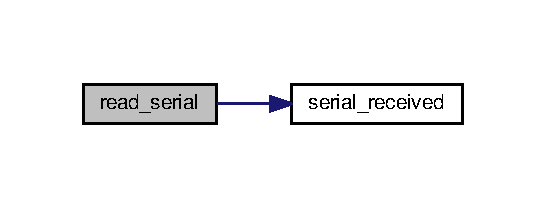
\includegraphics[width=262pt]{serial_8h_ab3b28cf37d70288fb56ad06c1815d824_cgraph}
\end{center}
\end{figure}
\mbox{\Hypertarget{serial_8h_a94affa1c8d77a69875f10c4915614afe}\label{serial_8h_a94affa1c8d77a69875f10c4915614afe}} 
\index{serial.\+h@{serial.\+h}!serial\+\_\+put\+\_\+char@{serial\+\_\+put\+\_\+char}}
\index{serial\+\_\+put\+\_\+char@{serial\+\_\+put\+\_\+char}!serial.\+h@{serial.\+h}}
\subsubsection{\texorpdfstring{serial\+\_\+put\+\_\+char()}{serial\_put\_char()}}
{\footnotesize\ttfamily void serial\+\_\+put\+\_\+char (\begin{DoxyParamCaption}\item[{const char}]{character }\end{DoxyParamCaption})}

Here is the call graph for this function\+:\nopagebreak
\begin{figure}[H]
\begin{center}
\leavevmode
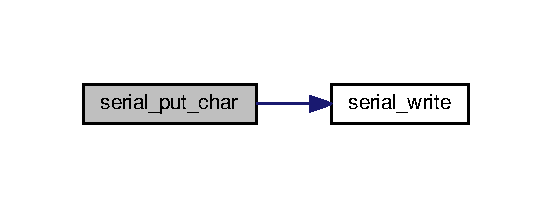
\includegraphics[width=265pt]{serial_8h_a94affa1c8d77a69875f10c4915614afe_cgraph}
\end{center}
\end{figure}
\mbox{\Hypertarget{serial_8h_a89ce044b86475f9d3e3688b7cb043cc8}\label{serial_8h_a89ce044b86475f9d3e3688b7cb043cc8}} 
\index{serial.\+h@{serial.\+h}!serial\+\_\+put\+\_\+string@{serial\+\_\+put\+\_\+string}}
\index{serial\+\_\+put\+\_\+string@{serial\+\_\+put\+\_\+string}!serial.\+h@{serial.\+h}}
\subsubsection{\texorpdfstring{serial\+\_\+put\+\_\+string()}{serial\_put\_string()}}
{\footnotesize\ttfamily void serial\+\_\+put\+\_\+string (\begin{DoxyParamCaption}\item[{const char $\ast$}]{string }\end{DoxyParamCaption})}

Here is the call graph for this function\+:\nopagebreak
\begin{figure}[H]
\begin{center}
\leavevmode
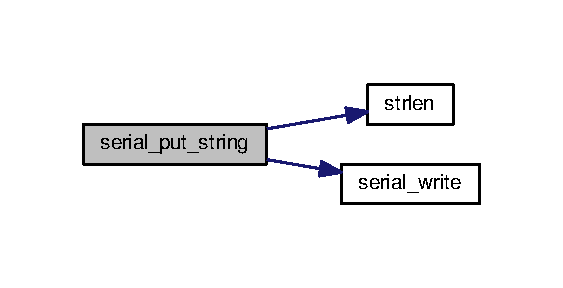
\includegraphics[width=270pt]{serial_8h_a89ce044b86475f9d3e3688b7cb043cc8_cgraph}
\end{center}
\end{figure}
\mbox{\Hypertarget{serial_8h_a45e1160c98d53c1306e75a32d54e81a3}\label{serial_8h_a45e1160c98d53c1306e75a32d54e81a3}} 
\index{serial.\+h@{serial.\+h}!serial\+\_\+received@{serial\+\_\+received}}
\index{serial\+\_\+received@{serial\+\_\+received}!serial.\+h@{serial.\+h}}
\subsubsection{\texorpdfstring{serial\+\_\+received()}{serial\_received()}}
{\footnotesize\ttfamily \hyperlink{stdint_8h_aba7bc1797add20fe3efdf37ced1182c5}{uint8\+\_\+t} serial\+\_\+received (\begin{DoxyParamCaption}\item[{const \hyperlink{stdint_8h_a324c5d28c0d82f502a234ab99efac87a}{uint32\+\_\+t}}]{port }\end{DoxyParamCaption})}

Here is the caller graph for this function\+:\nopagebreak
\begin{figure}[H]
\begin{center}
\leavevmode
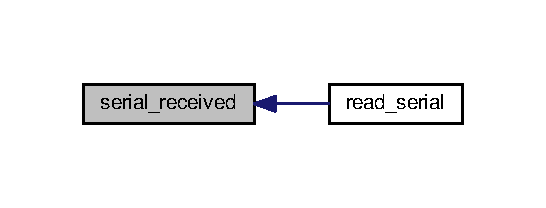
\includegraphics[width=262pt]{serial_8h_a45e1160c98d53c1306e75a32d54e81a3_icgraph}
\end{center}
\end{figure}
\mbox{\Hypertarget{serial_8h_afb7bd137c3cca6f25fb34170ff58c999}\label{serial_8h_afb7bd137c3cca6f25fb34170ff58c999}} 
\index{serial.\+h@{serial.\+h}!serial\+\_\+write@{serial\+\_\+write}}
\index{serial\+\_\+write@{serial\+\_\+write}!serial.\+h@{serial.\+h}}
\subsubsection{\texorpdfstring{serial\+\_\+write()}{serial\_write()}}
{\footnotesize\ttfamily void serial\+\_\+write (\begin{DoxyParamCaption}\item[{const \hyperlink{stdint_8h_a324c5d28c0d82f502a234ab99efac87a}{uint32\+\_\+t}}]{port,  }\item[{const \hyperlink{stdint_8h_aba7bc1797add20fe3efdf37ced1182c5}{uint8\+\_\+t}}]{data }\end{DoxyParamCaption})}

Here is the caller graph for this function\+:\nopagebreak
\begin{figure}[H]
\begin{center}
\leavevmode
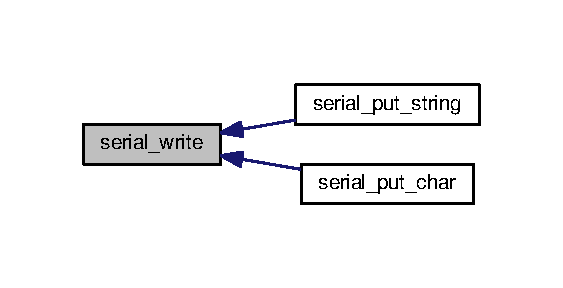
\includegraphics[width=270pt]{serial_8h_afb7bd137c3cca6f25fb34170ff58c999_icgraph}
\end{center}
\end{figure}

\hypertarget{vga__text_8h}{}\section{/home/alexy/\+Documents/\+Dev/\+R\+T\+L\+K\+I\+M/\+Source/\+Includes/\+Drivers/vga\+\_\+text.h File Reference}
\label{vga__text_8h}\index{/home/alexy/\+Documents/\+Dev/\+R\+T\+L\+K\+I\+M/\+Source/\+Includes/\+Drivers/vga\+\_\+text.\+h@{/home/alexy/\+Documents/\+Dev/\+R\+T\+L\+K\+I\+M/\+Source/\+Includes/\+Drivers/vga\+\_\+text.\+h}}
{\ttfamily \#include $<$Lib/stdint.\+h$>$}\newline
{\ttfamily \#include $<$Lib/stddef.\+h$>$}\newline
{\ttfamily \#include $<$Drivers/graphic.\+h$>$}\newline
Include dependency graph for vga\+\_\+text.\+h\+:\nopagebreak
\begin{figure}[H]
\begin{center}
\leavevmode
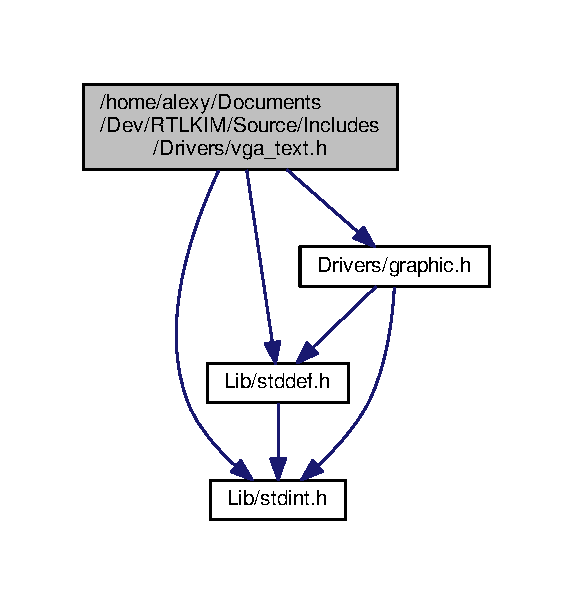
\includegraphics[width=275pt]{vga__text_8h__incl}
\end{center}
\end{figure}
This graph shows which files directly or indirectly include this file\+:\nopagebreak
\begin{figure}[H]
\begin{center}
\leavevmode
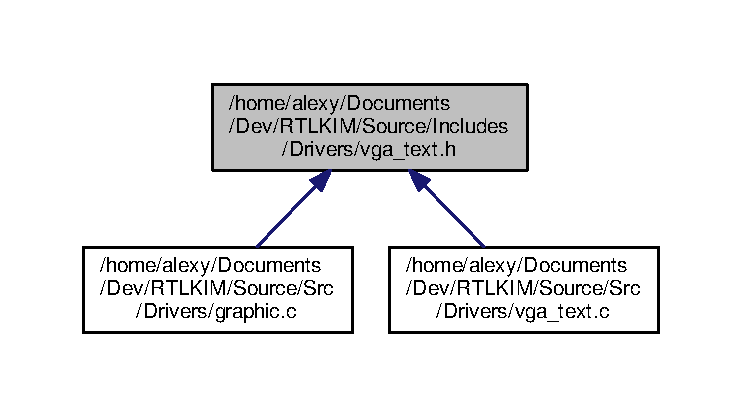
\includegraphics[width=350pt]{vga__text_8h__dep__incl}
\end{center}
\end{figure}
\subsection*{Macros}
\begin{DoxyCompactItemize}
\item 
\#define \hyperlink{vga__text_8h_a560ab135e02e199224d5ba1e33e1c2c6}{V\+G\+A\+\_\+\+T\+E\+X\+T\+\_\+\+F\+R\+A\+M\+E\+B\+U\+F\+F\+ER}~0x\+B8000
\item 
\#define \hyperlink{vga__text_8h_a3956e1761cb986b9589926db44b596a3}{S\+C\+R\+E\+E\+N\+\_\+\+D\+A\+T\+A\+\_\+\+P\+O\+RT}~0x3\+D5
\item 
\#define \hyperlink{vga__text_8h_a8b2ba16a5cda1f349eddf7913d78576f}{S\+C\+R\+E\+E\+N\+\_\+\+C\+O\+M\+M\+\_\+\+P\+O\+RT}~0x3\+D4
\item 
\#define \hyperlink{vga__text_8h_a8711c587c29239890d944dcbdf89fa85}{S\+C\+R\+E\+E\+N\+\_\+\+C\+O\+L\+\_\+\+S\+I\+ZE}~80
\item 
\#define \hyperlink{vga__text_8h_af8554d69af1411bc5fc5fae18694f2ca}{S\+C\+R\+E\+E\+N\+\_\+\+L\+I\+N\+E\+\_\+\+S\+I\+ZE}~25
\item 
\#define \hyperlink{vga__text_8h_a1483089752fb60bbe8e653b7cce45d0e}{C\+U\+R\+S\+O\+R\+\_\+\+C\+O\+M\+M\+\_\+\+L\+OW}~0x0F
\item 
\#define \hyperlink{vga__text_8h_afa6e00e5aab404ffb80738a80b6a9ba5}{C\+U\+R\+S\+O\+R\+\_\+\+C\+O\+M\+M\+\_\+\+H\+I\+GH}~0x0E
\end{DoxyCompactItemize}
\subsection*{Functions}
\begin{DoxyCompactItemize}
\item 
\hyperlink{stdint_8h_a273cf69d639a59973b6019625df33e30}{uint16\+\_\+t} $\ast$ \hyperlink{vga__text_8h_a210d07f3cb89bdcc879fbc108a7e38c6}{vga\+\_\+get\+\_\+framebuffer} (const \hyperlink{stdint_8h_aba7bc1797add20fe3efdf37ced1182c5}{uint8\+\_\+t} line, const \hyperlink{stdint_8h_aba7bc1797add20fe3efdf37ced1182c5}{uint8\+\_\+t} column)
\item 
void \hyperlink{vga__text_8h_a2b09cc380d21fec36e35fe1f45911d60}{vga\+\_\+clear\+\_\+screen} (void)
\item 
\hyperlink{stddef_8h_a51557cb52bbb9ee9d55aab5b9b16c3d0}{O\+S\+\_\+\+R\+E\+T\+U\+R\+N\+\_\+E} \hyperlink{vga__text_8h_ac4a8f5db75c8b03734d8f08f1bd314f2}{vga\+\_\+put\+\_\+cursor\+\_\+at} (const \hyperlink{stdint_8h_aba7bc1797add20fe3efdf37ced1182c5}{uint8\+\_\+t} line, const \hyperlink{stdint_8h_aba7bc1797add20fe3efdf37ced1182c5}{uint8\+\_\+t} column)
\item 
\hyperlink{stddef_8h_a51557cb52bbb9ee9d55aab5b9b16c3d0}{O\+S\+\_\+\+R\+E\+T\+U\+R\+N\+\_\+E} \hyperlink{vga__text_8h_a1741b2030e84c9dece9d3057742b903d}{vga\+\_\+save\+\_\+cursor} (\hyperlink{graphic_8h_a2377a22e1ea925fc95c5ec7b5bea95f5}{cursor\+\_\+t} $\ast$buffer)
\item 
\hyperlink{stddef_8h_a51557cb52bbb9ee9d55aab5b9b16c3d0}{O\+S\+\_\+\+R\+E\+T\+U\+R\+N\+\_\+E} \hyperlink{vga__text_8h_a75c08436c0a7c79dba855c8730d433d7}{vga\+\_\+restore\+\_\+cursor} (const \hyperlink{graphic_8h_a2377a22e1ea925fc95c5ec7b5bea95f5}{cursor\+\_\+t} buffer)
\item 
void \hyperlink{vga__text_8h_ac336eaf6527433256f31fc9270a7c855}{vga\+\_\+scroll} (const \hyperlink{graphic_8h_a223e9e8985b8d61206bd7628103b726f}{S\+C\+R\+O\+L\+L\+\_\+\+D\+I\+R\+E\+C\+T\+I\+O\+N\+\_\+E} direction, const \hyperlink{stdint_8h_aba7bc1797add20fe3efdf37ced1182c5}{uint8\+\_\+t} lines\+\_\+count)
\item 
void \hyperlink{vga__text_8h_a7abb70fbaa781f2e16ca29709f978fec}{vga\+\_\+set\+\_\+color\+\_\+scheme} (const \hyperlink{graphic_8h_ad71288aca9a1e3d064316c1072f04bb7}{colorscheme\+\_\+t} color\+\_\+sheme)
\item 
\hyperlink{stddef_8h_a51557cb52bbb9ee9d55aab5b9b16c3d0}{O\+S\+\_\+\+R\+E\+T\+U\+R\+N\+\_\+E} \hyperlink{vga__text_8h_a73e20c6187f2459590b0e6849270f4c1}{vga\+\_\+save\+\_\+color\+\_\+scheme} (\hyperlink{graphic_8h_ad71288aca9a1e3d064316c1072f04bb7}{colorscheme\+\_\+t} $\ast$buffer)
\item 
void \hyperlink{vga__text_8h_ac42a5001b2882a045425278d98c21bcd}{vga\+\_\+put\+\_\+string} (const char $\ast$string)
\item 
void \hyperlink{vga__text_8h_a284468b1478c8c91ff30f29c2d766ae5}{vga\+\_\+put\+\_\+char} (const char character)
\item 
void \hyperlink{vga__text_8h_acf23a9e1de51241d02f0ad476baf866b}{vga\+\_\+console\+\_\+write\+\_\+keyboard} (const char $\ast$str, const \hyperlink{stdint_8h_a324c5d28c0d82f502a234ab99efac87a}{uint32\+\_\+t} len)
\end{DoxyCompactItemize}


\subsection{Macro Definition Documentation}
\mbox{\Hypertarget{vga__text_8h_afa6e00e5aab404ffb80738a80b6a9ba5}\label{vga__text_8h_afa6e00e5aab404ffb80738a80b6a9ba5}} 
\index{vga\+\_\+text.\+h@{vga\+\_\+text.\+h}!C\+U\+R\+S\+O\+R\+\_\+\+C\+O\+M\+M\+\_\+\+H\+I\+GH@{C\+U\+R\+S\+O\+R\+\_\+\+C\+O\+M\+M\+\_\+\+H\+I\+GH}}
\index{C\+U\+R\+S\+O\+R\+\_\+\+C\+O\+M\+M\+\_\+\+H\+I\+GH@{C\+U\+R\+S\+O\+R\+\_\+\+C\+O\+M\+M\+\_\+\+H\+I\+GH}!vga\+\_\+text.\+h@{vga\+\_\+text.\+h}}
\subsubsection{\texorpdfstring{C\+U\+R\+S\+O\+R\+\_\+\+C\+O\+M\+M\+\_\+\+H\+I\+GH}{CURSOR\_COMM\_HIGH}}
{\footnotesize\ttfamily \#define C\+U\+R\+S\+O\+R\+\_\+\+C\+O\+M\+M\+\_\+\+H\+I\+GH~0x0E}

\mbox{\Hypertarget{vga__text_8h_a1483089752fb60bbe8e653b7cce45d0e}\label{vga__text_8h_a1483089752fb60bbe8e653b7cce45d0e}} 
\index{vga\+\_\+text.\+h@{vga\+\_\+text.\+h}!C\+U\+R\+S\+O\+R\+\_\+\+C\+O\+M\+M\+\_\+\+L\+OW@{C\+U\+R\+S\+O\+R\+\_\+\+C\+O\+M\+M\+\_\+\+L\+OW}}
\index{C\+U\+R\+S\+O\+R\+\_\+\+C\+O\+M\+M\+\_\+\+L\+OW@{C\+U\+R\+S\+O\+R\+\_\+\+C\+O\+M\+M\+\_\+\+L\+OW}!vga\+\_\+text.\+h@{vga\+\_\+text.\+h}}
\subsubsection{\texorpdfstring{C\+U\+R\+S\+O\+R\+\_\+\+C\+O\+M\+M\+\_\+\+L\+OW}{CURSOR\_COMM\_LOW}}
{\footnotesize\ttfamily \#define C\+U\+R\+S\+O\+R\+\_\+\+C\+O\+M\+M\+\_\+\+L\+OW~0x0F}

\mbox{\Hypertarget{vga__text_8h_a8711c587c29239890d944dcbdf89fa85}\label{vga__text_8h_a8711c587c29239890d944dcbdf89fa85}} 
\index{vga\+\_\+text.\+h@{vga\+\_\+text.\+h}!S\+C\+R\+E\+E\+N\+\_\+\+C\+O\+L\+\_\+\+S\+I\+ZE@{S\+C\+R\+E\+E\+N\+\_\+\+C\+O\+L\+\_\+\+S\+I\+ZE}}
\index{S\+C\+R\+E\+E\+N\+\_\+\+C\+O\+L\+\_\+\+S\+I\+ZE@{S\+C\+R\+E\+E\+N\+\_\+\+C\+O\+L\+\_\+\+S\+I\+ZE}!vga\+\_\+text.\+h@{vga\+\_\+text.\+h}}
\subsubsection{\texorpdfstring{S\+C\+R\+E\+E\+N\+\_\+\+C\+O\+L\+\_\+\+S\+I\+ZE}{SCREEN\_COL\_SIZE}}
{\footnotesize\ttfamily \#define S\+C\+R\+E\+E\+N\+\_\+\+C\+O\+L\+\_\+\+S\+I\+ZE~80}

\mbox{\Hypertarget{vga__text_8h_a8b2ba16a5cda1f349eddf7913d78576f}\label{vga__text_8h_a8b2ba16a5cda1f349eddf7913d78576f}} 
\index{vga\+\_\+text.\+h@{vga\+\_\+text.\+h}!S\+C\+R\+E\+E\+N\+\_\+\+C\+O\+M\+M\+\_\+\+P\+O\+RT@{S\+C\+R\+E\+E\+N\+\_\+\+C\+O\+M\+M\+\_\+\+P\+O\+RT}}
\index{S\+C\+R\+E\+E\+N\+\_\+\+C\+O\+M\+M\+\_\+\+P\+O\+RT@{S\+C\+R\+E\+E\+N\+\_\+\+C\+O\+M\+M\+\_\+\+P\+O\+RT}!vga\+\_\+text.\+h@{vga\+\_\+text.\+h}}
\subsubsection{\texorpdfstring{S\+C\+R\+E\+E\+N\+\_\+\+C\+O\+M\+M\+\_\+\+P\+O\+RT}{SCREEN\_COMM\_PORT}}
{\footnotesize\ttfamily \#define S\+C\+R\+E\+E\+N\+\_\+\+C\+O\+M\+M\+\_\+\+P\+O\+RT~0x3\+D4}

\mbox{\Hypertarget{vga__text_8h_a3956e1761cb986b9589926db44b596a3}\label{vga__text_8h_a3956e1761cb986b9589926db44b596a3}} 
\index{vga\+\_\+text.\+h@{vga\+\_\+text.\+h}!S\+C\+R\+E\+E\+N\+\_\+\+D\+A\+T\+A\+\_\+\+P\+O\+RT@{S\+C\+R\+E\+E\+N\+\_\+\+D\+A\+T\+A\+\_\+\+P\+O\+RT}}
\index{S\+C\+R\+E\+E\+N\+\_\+\+D\+A\+T\+A\+\_\+\+P\+O\+RT@{S\+C\+R\+E\+E\+N\+\_\+\+D\+A\+T\+A\+\_\+\+P\+O\+RT}!vga\+\_\+text.\+h@{vga\+\_\+text.\+h}}
\subsubsection{\texorpdfstring{S\+C\+R\+E\+E\+N\+\_\+\+D\+A\+T\+A\+\_\+\+P\+O\+RT}{SCREEN\_DATA\_PORT}}
{\footnotesize\ttfamily \#define S\+C\+R\+E\+E\+N\+\_\+\+D\+A\+T\+A\+\_\+\+P\+O\+RT~0x3\+D5}

\mbox{\Hypertarget{vga__text_8h_af8554d69af1411bc5fc5fae18694f2ca}\label{vga__text_8h_af8554d69af1411bc5fc5fae18694f2ca}} 
\index{vga\+\_\+text.\+h@{vga\+\_\+text.\+h}!S\+C\+R\+E\+E\+N\+\_\+\+L\+I\+N\+E\+\_\+\+S\+I\+ZE@{S\+C\+R\+E\+E\+N\+\_\+\+L\+I\+N\+E\+\_\+\+S\+I\+ZE}}
\index{S\+C\+R\+E\+E\+N\+\_\+\+L\+I\+N\+E\+\_\+\+S\+I\+ZE@{S\+C\+R\+E\+E\+N\+\_\+\+L\+I\+N\+E\+\_\+\+S\+I\+ZE}!vga\+\_\+text.\+h@{vga\+\_\+text.\+h}}
\subsubsection{\texorpdfstring{S\+C\+R\+E\+E\+N\+\_\+\+L\+I\+N\+E\+\_\+\+S\+I\+ZE}{SCREEN\_LINE\_SIZE}}
{\footnotesize\ttfamily \#define S\+C\+R\+E\+E\+N\+\_\+\+L\+I\+N\+E\+\_\+\+S\+I\+ZE~25}

\mbox{\Hypertarget{vga__text_8h_a560ab135e02e199224d5ba1e33e1c2c6}\label{vga__text_8h_a560ab135e02e199224d5ba1e33e1c2c6}} 
\index{vga\+\_\+text.\+h@{vga\+\_\+text.\+h}!V\+G\+A\+\_\+\+T\+E\+X\+T\+\_\+\+F\+R\+A\+M\+E\+B\+U\+F\+F\+ER@{V\+G\+A\+\_\+\+T\+E\+X\+T\+\_\+\+F\+R\+A\+M\+E\+B\+U\+F\+F\+ER}}
\index{V\+G\+A\+\_\+\+T\+E\+X\+T\+\_\+\+F\+R\+A\+M\+E\+B\+U\+F\+F\+ER@{V\+G\+A\+\_\+\+T\+E\+X\+T\+\_\+\+F\+R\+A\+M\+E\+B\+U\+F\+F\+ER}!vga\+\_\+text.\+h@{vga\+\_\+text.\+h}}
\subsubsection{\texorpdfstring{V\+G\+A\+\_\+\+T\+E\+X\+T\+\_\+\+F\+R\+A\+M\+E\+B\+U\+F\+F\+ER}{VGA\_TEXT\_FRAMEBUFFER}}
{\footnotesize\ttfamily \#define V\+G\+A\+\_\+\+T\+E\+X\+T\+\_\+\+F\+R\+A\+M\+E\+B\+U\+F\+F\+ER~0x\+B8000}



\subsection{Function Documentation}
\mbox{\Hypertarget{vga__text_8h_a2b09cc380d21fec36e35fe1f45911d60}\label{vga__text_8h_a2b09cc380d21fec36e35fe1f45911d60}} 
\index{vga\+\_\+text.\+h@{vga\+\_\+text.\+h}!vga\+\_\+clear\+\_\+screen@{vga\+\_\+clear\+\_\+screen}}
\index{vga\+\_\+clear\+\_\+screen@{vga\+\_\+clear\+\_\+screen}!vga\+\_\+text.\+h@{vga\+\_\+text.\+h}}
\subsubsection{\texorpdfstring{vga\+\_\+clear\+\_\+screen()}{vga\_clear\_screen()}}
{\footnotesize\ttfamily void vga\+\_\+clear\+\_\+screen (\begin{DoxyParamCaption}\item[{void}]{ }\end{DoxyParamCaption})}

Here is the call graph for this function\+:\nopagebreak
\begin{figure}[H]
\begin{center}
\leavevmode
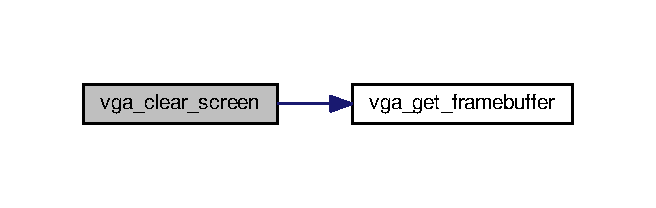
\includegraphics[width=315pt]{vga__text_8h_a2b09cc380d21fec36e35fe1f45911d60_cgraph}
\end{center}
\end{figure}
Here is the caller graph for this function\+:\nopagebreak
\begin{figure}[H]
\begin{center}
\leavevmode
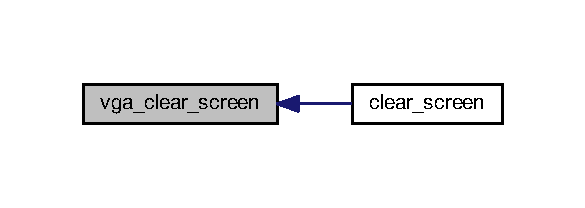
\includegraphics[width=281pt]{vga__text_8h_a2b09cc380d21fec36e35fe1f45911d60_icgraph}
\end{center}
\end{figure}
\mbox{\Hypertarget{vga__text_8h_acf23a9e1de51241d02f0ad476baf866b}\label{vga__text_8h_acf23a9e1de51241d02f0ad476baf866b}} 
\index{vga\+\_\+text.\+h@{vga\+\_\+text.\+h}!vga\+\_\+console\+\_\+write\+\_\+keyboard@{vga\+\_\+console\+\_\+write\+\_\+keyboard}}
\index{vga\+\_\+console\+\_\+write\+\_\+keyboard@{vga\+\_\+console\+\_\+write\+\_\+keyboard}!vga\+\_\+text.\+h@{vga\+\_\+text.\+h}}
\subsubsection{\texorpdfstring{vga\+\_\+console\+\_\+write\+\_\+keyboard()}{vga\_console\_write\_keyboard()}}
{\footnotesize\ttfamily void vga\+\_\+console\+\_\+write\+\_\+keyboard (\begin{DoxyParamCaption}\item[{const char $\ast$}]{str,  }\item[{const \hyperlink{stdint_8h_a324c5d28c0d82f502a234ab99efac87a}{uint32\+\_\+t}}]{len }\end{DoxyParamCaption})}

Here is the caller graph for this function\+:\nopagebreak
\begin{figure}[H]
\begin{center}
\leavevmode
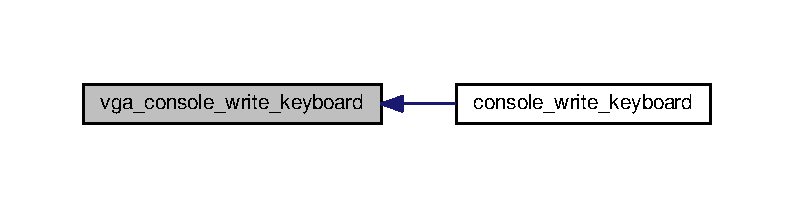
\includegraphics[width=350pt]{vga__text_8h_acf23a9e1de51241d02f0ad476baf866b_icgraph}
\end{center}
\end{figure}
\mbox{\Hypertarget{vga__text_8h_a210d07f3cb89bdcc879fbc108a7e38c6}\label{vga__text_8h_a210d07f3cb89bdcc879fbc108a7e38c6}} 
\index{vga\+\_\+text.\+h@{vga\+\_\+text.\+h}!vga\+\_\+get\+\_\+framebuffer@{vga\+\_\+get\+\_\+framebuffer}}
\index{vga\+\_\+get\+\_\+framebuffer@{vga\+\_\+get\+\_\+framebuffer}!vga\+\_\+text.\+h@{vga\+\_\+text.\+h}}
\subsubsection{\texorpdfstring{vga\+\_\+get\+\_\+framebuffer()}{vga\_get\_framebuffer()}}
{\footnotesize\ttfamily \hyperlink{stdint_8h_a273cf69d639a59973b6019625df33e30}{uint16\+\_\+t}$\ast$ vga\+\_\+get\+\_\+framebuffer (\begin{DoxyParamCaption}\item[{const \hyperlink{stdint_8h_aba7bc1797add20fe3efdf37ced1182c5}{uint8\+\_\+t}}]{line,  }\item[{const \hyperlink{stdint_8h_aba7bc1797add20fe3efdf37ced1182c5}{uint8\+\_\+t}}]{column }\end{DoxyParamCaption})}

Here is the caller graph for this function\+:\nopagebreak
\begin{figure}[H]
\begin{center}
\leavevmode
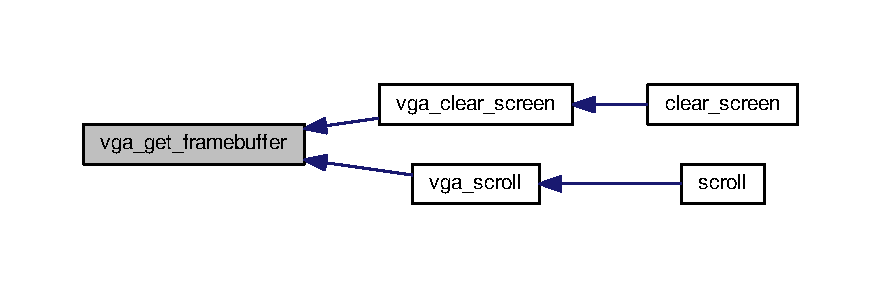
\includegraphics[width=350pt]{vga__text_8h_a210d07f3cb89bdcc879fbc108a7e38c6_icgraph}
\end{center}
\end{figure}
\mbox{\Hypertarget{vga__text_8h_a284468b1478c8c91ff30f29c2d766ae5}\label{vga__text_8h_a284468b1478c8c91ff30f29c2d766ae5}} 
\index{vga\+\_\+text.\+h@{vga\+\_\+text.\+h}!vga\+\_\+put\+\_\+char@{vga\+\_\+put\+\_\+char}}
\index{vga\+\_\+put\+\_\+char@{vga\+\_\+put\+\_\+char}!vga\+\_\+text.\+h@{vga\+\_\+text.\+h}}
\subsubsection{\texorpdfstring{vga\+\_\+put\+\_\+char()}{vga\_put\_char()}}
{\footnotesize\ttfamily void vga\+\_\+put\+\_\+char (\begin{DoxyParamCaption}\item[{const char}]{character }\end{DoxyParamCaption})}

Here is the caller graph for this function\+:\nopagebreak
\begin{figure}[H]
\begin{center}
\leavevmode
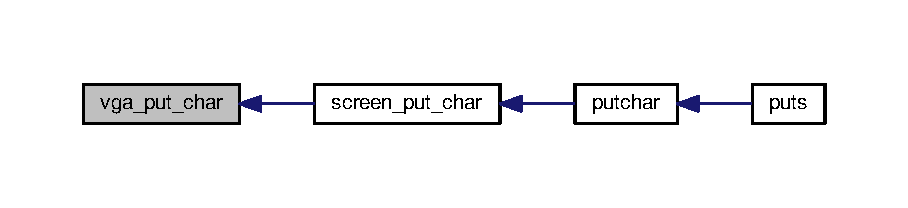
\includegraphics[width=350pt]{vga__text_8h_a284468b1478c8c91ff30f29c2d766ae5_icgraph}
\end{center}
\end{figure}
\mbox{\Hypertarget{vga__text_8h_ac4a8f5db75c8b03734d8f08f1bd314f2}\label{vga__text_8h_ac4a8f5db75c8b03734d8f08f1bd314f2}} 
\index{vga\+\_\+text.\+h@{vga\+\_\+text.\+h}!vga\+\_\+put\+\_\+cursor\+\_\+at@{vga\+\_\+put\+\_\+cursor\+\_\+at}}
\index{vga\+\_\+put\+\_\+cursor\+\_\+at@{vga\+\_\+put\+\_\+cursor\+\_\+at}!vga\+\_\+text.\+h@{vga\+\_\+text.\+h}}
\subsubsection{\texorpdfstring{vga\+\_\+put\+\_\+cursor\+\_\+at()}{vga\_put\_cursor\_at()}}
{\footnotesize\ttfamily \hyperlink{stddef_8h_a51557cb52bbb9ee9d55aab5b9b16c3d0}{O\+S\+\_\+\+R\+E\+T\+U\+R\+N\+\_\+E} vga\+\_\+put\+\_\+cursor\+\_\+at (\begin{DoxyParamCaption}\item[{const \hyperlink{stdint_8h_aba7bc1797add20fe3efdf37ced1182c5}{uint8\+\_\+t}}]{line,  }\item[{const \hyperlink{stdint_8h_aba7bc1797add20fe3efdf37ced1182c5}{uint8\+\_\+t}}]{column }\end{DoxyParamCaption})}

Here is the caller graph for this function\+:\nopagebreak
\begin{figure}[H]
\begin{center}
\leavevmode
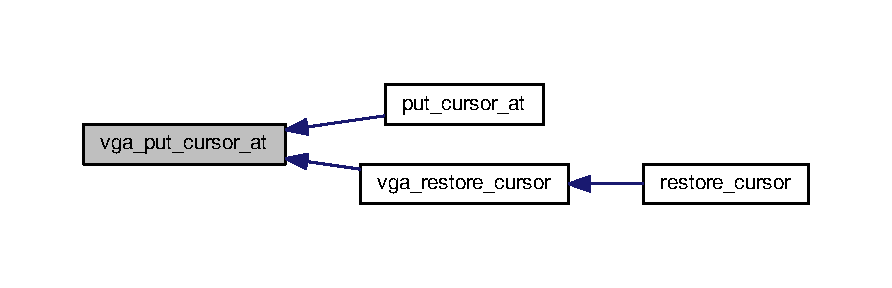
\includegraphics[width=350pt]{vga__text_8h_ac4a8f5db75c8b03734d8f08f1bd314f2_icgraph}
\end{center}
\end{figure}
\mbox{\Hypertarget{vga__text_8h_ac42a5001b2882a045425278d98c21bcd}\label{vga__text_8h_ac42a5001b2882a045425278d98c21bcd}} 
\index{vga\+\_\+text.\+h@{vga\+\_\+text.\+h}!vga\+\_\+put\+\_\+string@{vga\+\_\+put\+\_\+string}}
\index{vga\+\_\+put\+\_\+string@{vga\+\_\+put\+\_\+string}!vga\+\_\+text.\+h@{vga\+\_\+text.\+h}}
\subsubsection{\texorpdfstring{vga\+\_\+put\+\_\+string()}{vga\_put\_string()}}
{\footnotesize\ttfamily void vga\+\_\+put\+\_\+string (\begin{DoxyParamCaption}\item[{const char $\ast$}]{string }\end{DoxyParamCaption})}

Here is the call graph for this function\+:\nopagebreak
\begin{figure}[H]
\begin{center}
\leavevmode
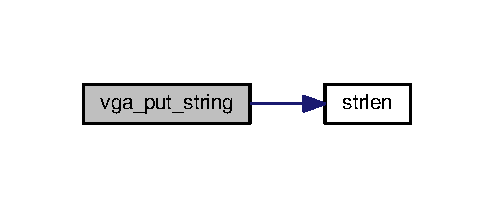
\includegraphics[width=237pt]{vga__text_8h_ac42a5001b2882a045425278d98c21bcd_cgraph}
\end{center}
\end{figure}
Here is the caller graph for this function\+:\nopagebreak
\begin{figure}[H]
\begin{center}
\leavevmode
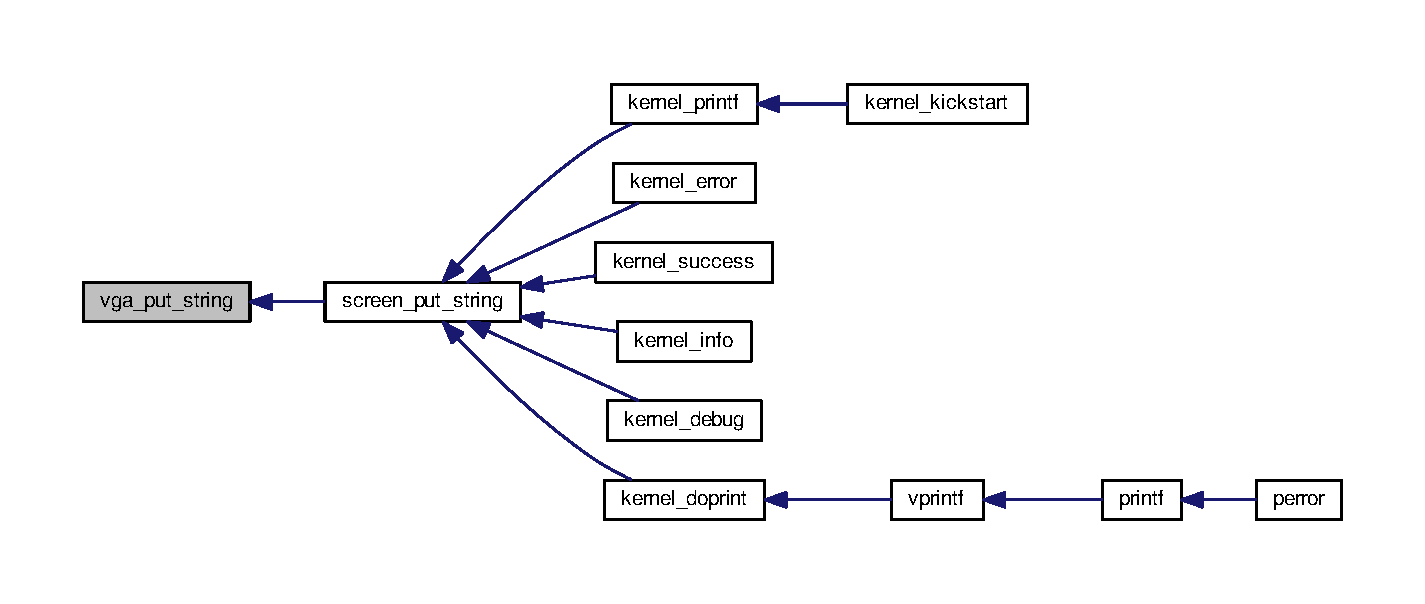
\includegraphics[width=350pt]{vga__text_8h_ac42a5001b2882a045425278d98c21bcd_icgraph}
\end{center}
\end{figure}
\mbox{\Hypertarget{vga__text_8h_a75c08436c0a7c79dba855c8730d433d7}\label{vga__text_8h_a75c08436c0a7c79dba855c8730d433d7}} 
\index{vga\+\_\+text.\+h@{vga\+\_\+text.\+h}!vga\+\_\+restore\+\_\+cursor@{vga\+\_\+restore\+\_\+cursor}}
\index{vga\+\_\+restore\+\_\+cursor@{vga\+\_\+restore\+\_\+cursor}!vga\+\_\+text.\+h@{vga\+\_\+text.\+h}}
\subsubsection{\texorpdfstring{vga\+\_\+restore\+\_\+cursor()}{vga\_restore\_cursor()}}
{\footnotesize\ttfamily \hyperlink{stddef_8h_a51557cb52bbb9ee9d55aab5b9b16c3d0}{O\+S\+\_\+\+R\+E\+T\+U\+R\+N\+\_\+E} vga\+\_\+restore\+\_\+cursor (\begin{DoxyParamCaption}\item[{const \hyperlink{graphic_8h_a2377a22e1ea925fc95c5ec7b5bea95f5}{cursor\+\_\+t}}]{buffer }\end{DoxyParamCaption})}

Here is the call graph for this function\+:\nopagebreak
\begin{figure}[H]
\begin{center}
\leavevmode
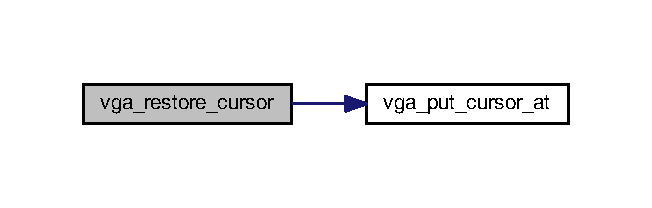
\includegraphics[width=313pt]{vga__text_8h_a75c08436c0a7c79dba855c8730d433d7_cgraph}
\end{center}
\end{figure}
Here is the caller graph for this function\+:\nopagebreak
\begin{figure}[H]
\begin{center}
\leavevmode
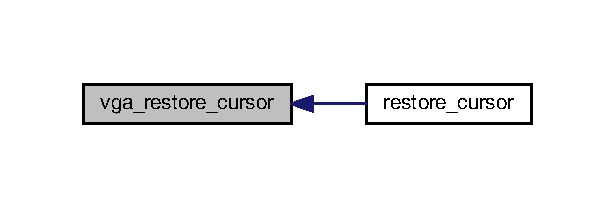
\includegraphics[width=295pt]{vga__text_8h_a75c08436c0a7c79dba855c8730d433d7_icgraph}
\end{center}
\end{figure}
\mbox{\Hypertarget{vga__text_8h_a73e20c6187f2459590b0e6849270f4c1}\label{vga__text_8h_a73e20c6187f2459590b0e6849270f4c1}} 
\index{vga\+\_\+text.\+h@{vga\+\_\+text.\+h}!vga\+\_\+save\+\_\+color\+\_\+scheme@{vga\+\_\+save\+\_\+color\+\_\+scheme}}
\index{vga\+\_\+save\+\_\+color\+\_\+scheme@{vga\+\_\+save\+\_\+color\+\_\+scheme}!vga\+\_\+text.\+h@{vga\+\_\+text.\+h}}
\subsubsection{\texorpdfstring{vga\+\_\+save\+\_\+color\+\_\+scheme()}{vga\_save\_color\_scheme()}}
{\footnotesize\ttfamily \hyperlink{stddef_8h_a51557cb52bbb9ee9d55aab5b9b16c3d0}{O\+S\+\_\+\+R\+E\+T\+U\+R\+N\+\_\+E} vga\+\_\+save\+\_\+color\+\_\+scheme (\begin{DoxyParamCaption}\item[{\hyperlink{graphic_8h_ad71288aca9a1e3d064316c1072f04bb7}{colorscheme\+\_\+t} $\ast$}]{buffer }\end{DoxyParamCaption})}

Here is the caller graph for this function\+:\nopagebreak
\begin{figure}[H]
\begin{center}
\leavevmode
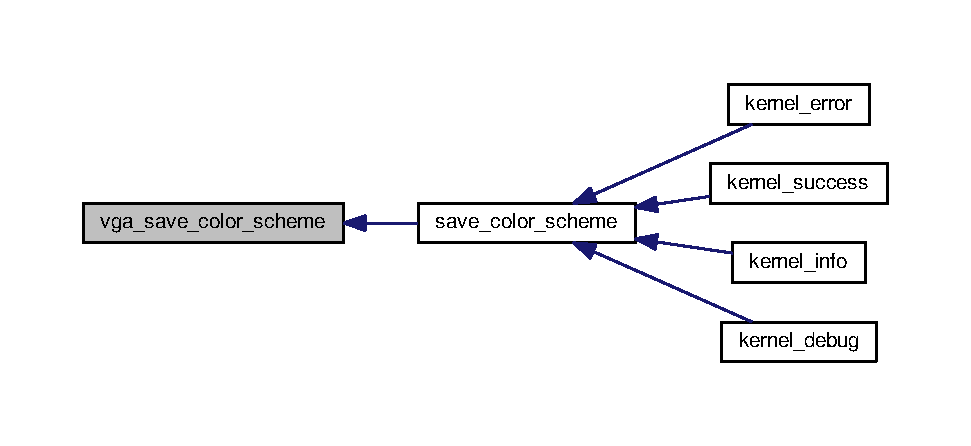
\includegraphics[width=350pt]{vga__text_8h_a73e20c6187f2459590b0e6849270f4c1_icgraph}
\end{center}
\end{figure}
\mbox{\Hypertarget{vga__text_8h_a1741b2030e84c9dece9d3057742b903d}\label{vga__text_8h_a1741b2030e84c9dece9d3057742b903d}} 
\index{vga\+\_\+text.\+h@{vga\+\_\+text.\+h}!vga\+\_\+save\+\_\+cursor@{vga\+\_\+save\+\_\+cursor}}
\index{vga\+\_\+save\+\_\+cursor@{vga\+\_\+save\+\_\+cursor}!vga\+\_\+text.\+h@{vga\+\_\+text.\+h}}
\subsubsection{\texorpdfstring{vga\+\_\+save\+\_\+cursor()}{vga\_save\_cursor()}}
{\footnotesize\ttfamily \hyperlink{stddef_8h_a51557cb52bbb9ee9d55aab5b9b16c3d0}{O\+S\+\_\+\+R\+E\+T\+U\+R\+N\+\_\+E} vga\+\_\+save\+\_\+cursor (\begin{DoxyParamCaption}\item[{\hyperlink{graphic_8h_a2377a22e1ea925fc95c5ec7b5bea95f5}{cursor\+\_\+t} $\ast$}]{buffer }\end{DoxyParamCaption})}

Here is the caller graph for this function\+:\nopagebreak
\begin{figure}[H]
\begin{center}
\leavevmode
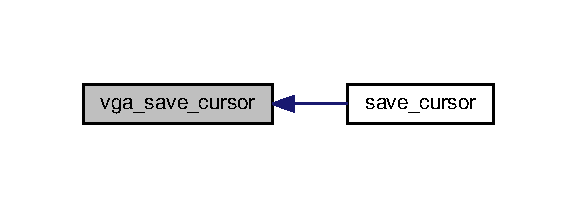
\includegraphics[width=277pt]{vga__text_8h_a1741b2030e84c9dece9d3057742b903d_icgraph}
\end{center}
\end{figure}
\mbox{\Hypertarget{vga__text_8h_ac336eaf6527433256f31fc9270a7c855}\label{vga__text_8h_ac336eaf6527433256f31fc9270a7c855}} 
\index{vga\+\_\+text.\+h@{vga\+\_\+text.\+h}!vga\+\_\+scroll@{vga\+\_\+scroll}}
\index{vga\+\_\+scroll@{vga\+\_\+scroll}!vga\+\_\+text.\+h@{vga\+\_\+text.\+h}}
\subsubsection{\texorpdfstring{vga\+\_\+scroll()}{vga\_scroll()}}
{\footnotesize\ttfamily void vga\+\_\+scroll (\begin{DoxyParamCaption}\item[{const \hyperlink{graphic_8h_a223e9e8985b8d61206bd7628103b726f}{S\+C\+R\+O\+L\+L\+\_\+\+D\+I\+R\+E\+C\+T\+I\+O\+N\+\_\+E}}]{direction,  }\item[{const \hyperlink{stdint_8h_aba7bc1797add20fe3efdf37ced1182c5}{uint8\+\_\+t}}]{lines\+\_\+count }\end{DoxyParamCaption})}

Here is the call graph for this function\+:\nopagebreak
\begin{figure}[H]
\begin{center}
\leavevmode
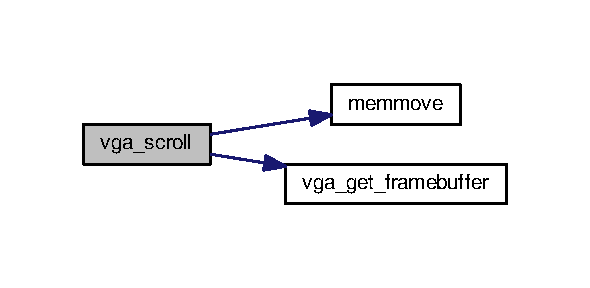
\includegraphics[width=283pt]{vga__text_8h_ac336eaf6527433256f31fc9270a7c855_cgraph}
\end{center}
\end{figure}
Here is the caller graph for this function\+:\nopagebreak
\begin{figure}[H]
\begin{center}
\leavevmode
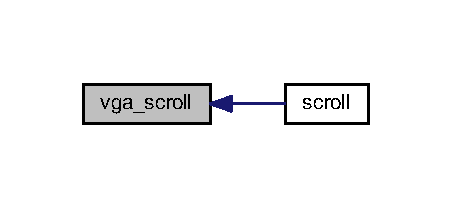
\includegraphics[width=217pt]{vga__text_8h_ac336eaf6527433256f31fc9270a7c855_icgraph}
\end{center}
\end{figure}
\mbox{\Hypertarget{vga__text_8h_a7abb70fbaa781f2e16ca29709f978fec}\label{vga__text_8h_a7abb70fbaa781f2e16ca29709f978fec}} 
\index{vga\+\_\+text.\+h@{vga\+\_\+text.\+h}!vga\+\_\+set\+\_\+color\+\_\+scheme@{vga\+\_\+set\+\_\+color\+\_\+scheme}}
\index{vga\+\_\+set\+\_\+color\+\_\+scheme@{vga\+\_\+set\+\_\+color\+\_\+scheme}!vga\+\_\+text.\+h@{vga\+\_\+text.\+h}}
\subsubsection{\texorpdfstring{vga\+\_\+set\+\_\+color\+\_\+scheme()}{vga\_set\_color\_scheme()}}
{\footnotesize\ttfamily void vga\+\_\+set\+\_\+color\+\_\+scheme (\begin{DoxyParamCaption}\item[{const \hyperlink{graphic_8h_ad71288aca9a1e3d064316c1072f04bb7}{colorscheme\+\_\+t}}]{color\+\_\+sheme }\end{DoxyParamCaption})}

Here is the caller graph for this function\+:\nopagebreak
\begin{figure}[H]
\begin{center}
\leavevmode
\includegraphics[width=350pt]{vga__text_8h_a7abb70fbaa781f2e16ca29709f978fec_icgraph}
\end{center}
\end{figure}

\hypertarget{kernel__output_8h}{}\section{/home/alexy/\+Documents/\+Dev/\+R\+T\+L\+K\+I\+M/\+Source/\+Includes/\+I\+O/kernel\+\_\+output.h File Reference}
\label{kernel__output_8h}\index{/home/alexy/\+Documents/\+Dev/\+R\+T\+L\+K\+I\+M/\+Source/\+Includes/\+I\+O/kernel\+\_\+output.\+h@{/home/alexy/\+Documents/\+Dev/\+R\+T\+L\+K\+I\+M/\+Source/\+Includes/\+I\+O/kernel\+\_\+output.\+h}}
This graph shows which files directly or indirectly include this file\+:\nopagebreak
\begin{figure}[H]
\begin{center}
\leavevmode
\includegraphics[width=350pt]{kernel__output_8h__dep__incl}
\end{center}
\end{figure}
\subsection*{Data Structures}
\begin{DoxyCompactItemize}
\item 
struct \hyperlink{structoutput}{output}
\end{DoxyCompactItemize}
\subsection*{Typedefs}
\begin{DoxyCompactItemize}
\item 
typedef struct \hyperlink{structoutput}{output} \hyperlink{kernel__output_8h_aa9d85a699dcab22f8641b751762edd16}{output\+\_\+t}
\end{DoxyCompactItemize}
\subsection*{Functions}
\begin{DoxyCompactItemize}
\item 
void \hyperlink{kernel__output_8h_ae0371f7a8b0f9c5fc52fec6482a4e697}{kernel\+\_\+printf} (const char $\ast$\+\_\+\+\_\+format,...)
\item 
void \hyperlink{kernel__output_8h_ac31be592ce4809152fd62b48ea16936b}{kernel\+\_\+error} (const char $\ast$\+\_\+\+\_\+format,...)
\item 
void \hyperlink{kernel__output_8h_a7e1efa0f9a0aa123e7676cac663f7831}{kernel\+\_\+success} (const char $\ast$\+\_\+\+\_\+format,...)
\item 
void \hyperlink{kernel__output_8h_a73639fcdfa7398ae4c2291cdcbd53e6d}{kernel\+\_\+info} (const char $\ast$\+\_\+\+\_\+format,...)
\item 
void \hyperlink{kernel__output_8h_af27e56178f3d404d4945635e572fdb90}{kernel\+\_\+debug} (const char $\ast$\+\_\+\+\_\+format,...)
\item 
void \hyperlink{kernel__output_8h_a45ccaf5c540696335ace382c031333c5}{kernel\+\_\+serial\+\_\+debug} (const char $\ast$\+\_\+\+\_\+format,...)
\item 
void \hyperlink{kernel__output_8h_ae9363952bbb60281d5b9069b485fb7a7}{kernel\+\_\+doprint} (const char $\ast$str, \+\_\+\+\_\+builtin\+\_\+va\+\_\+list args)
\end{DoxyCompactItemize}


\subsection{Typedef Documentation}
\mbox{\Hypertarget{kernel__output_8h_aa9d85a699dcab22f8641b751762edd16}\label{kernel__output_8h_aa9d85a699dcab22f8641b751762edd16}} 
\index{kernel\+\_\+output.\+h@{kernel\+\_\+output.\+h}!output\+\_\+t@{output\+\_\+t}}
\index{output\+\_\+t@{output\+\_\+t}!kernel\+\_\+output.\+h@{kernel\+\_\+output.\+h}}
\subsubsection{\texorpdfstring{output\+\_\+t}{output\_t}}
{\footnotesize\ttfamily typedef struct \hyperlink{structoutput}{output}  \hyperlink{kernel__output_8h_aa9d85a699dcab22f8641b751762edd16}{output\+\_\+t}}



\subsection{Function Documentation}
\mbox{\Hypertarget{kernel__output_8h_af27e56178f3d404d4945635e572fdb90}\label{kernel__output_8h_af27e56178f3d404d4945635e572fdb90}} 
\index{kernel\+\_\+output.\+h@{kernel\+\_\+output.\+h}!kernel\+\_\+debug@{kernel\+\_\+debug}}
\index{kernel\+\_\+debug@{kernel\+\_\+debug}!kernel\+\_\+output.\+h@{kernel\+\_\+output.\+h}}
\subsubsection{\texorpdfstring{kernel\+\_\+debug()}{kernel\_debug()}}
{\footnotesize\ttfamily void kernel\+\_\+debug (\begin{DoxyParamCaption}\item[{const char $\ast$}]{\+\_\+\+\_\+format,  }\item[{}]{... }\end{DoxyParamCaption})}

Here is the call graph for this function\+:\nopagebreak
\begin{figure}[H]
\begin{center}
\leavevmode
\includegraphics[width=350pt]{kernel__output_8h_af27e56178f3d404d4945635e572fdb90_cgraph}
\end{center}
\end{figure}
\mbox{\Hypertarget{kernel__output_8h_ae9363952bbb60281d5b9069b485fb7a7}\label{kernel__output_8h_ae9363952bbb60281d5b9069b485fb7a7}} 
\index{kernel\+\_\+output.\+h@{kernel\+\_\+output.\+h}!kernel\+\_\+doprint@{kernel\+\_\+doprint}}
\index{kernel\+\_\+doprint@{kernel\+\_\+doprint}!kernel\+\_\+output.\+h@{kernel\+\_\+output.\+h}}
\subsubsection{\texorpdfstring{kernel\+\_\+doprint()}{kernel\_doprint()}}
{\footnotesize\ttfamily void kernel\+\_\+doprint (\begin{DoxyParamCaption}\item[{const char $\ast$}]{str,  }\item[{\+\_\+\+\_\+builtin\+\_\+va\+\_\+list}]{args }\end{DoxyParamCaption})}

\mbox{\Hypertarget{kernel__output_8h_ac31be592ce4809152fd62b48ea16936b}\label{kernel__output_8h_ac31be592ce4809152fd62b48ea16936b}} 
\index{kernel\+\_\+output.\+h@{kernel\+\_\+output.\+h}!kernel\+\_\+error@{kernel\+\_\+error}}
\index{kernel\+\_\+error@{kernel\+\_\+error}!kernel\+\_\+output.\+h@{kernel\+\_\+output.\+h}}
\subsubsection{\texorpdfstring{kernel\+\_\+error()}{kernel\_error()}}
{\footnotesize\ttfamily void kernel\+\_\+error (\begin{DoxyParamCaption}\item[{const char $\ast$}]{\+\_\+\+\_\+format,  }\item[{}]{... }\end{DoxyParamCaption})}

\mbox{\Hypertarget{kernel__output_8h_a73639fcdfa7398ae4c2291cdcbd53e6d}\label{kernel__output_8h_a73639fcdfa7398ae4c2291cdcbd53e6d}} 
\index{kernel\+\_\+output.\+h@{kernel\+\_\+output.\+h}!kernel\+\_\+info@{kernel\+\_\+info}}
\index{kernel\+\_\+info@{kernel\+\_\+info}!kernel\+\_\+output.\+h@{kernel\+\_\+output.\+h}}
\subsubsection{\texorpdfstring{kernel\+\_\+info()}{kernel\_info()}}
{\footnotesize\ttfamily void kernel\+\_\+info (\begin{DoxyParamCaption}\item[{const char $\ast$}]{\+\_\+\+\_\+format,  }\item[{}]{... }\end{DoxyParamCaption})}

Here is the call graph for this function\+:\nopagebreak
\begin{figure}[H]
\begin{center}
\leavevmode
\includegraphics[width=350pt]{kernel__output_8h_a73639fcdfa7398ae4c2291cdcbd53e6d_cgraph}
\end{center}
\end{figure}
\mbox{\Hypertarget{kernel__output_8h_ae0371f7a8b0f9c5fc52fec6482a4e697}\label{kernel__output_8h_ae0371f7a8b0f9c5fc52fec6482a4e697}} 
\index{kernel\+\_\+output.\+h@{kernel\+\_\+output.\+h}!kernel\+\_\+printf@{kernel\+\_\+printf}}
\index{kernel\+\_\+printf@{kernel\+\_\+printf}!kernel\+\_\+output.\+h@{kernel\+\_\+output.\+h}}
\subsubsection{\texorpdfstring{kernel\+\_\+printf()}{kernel\_printf()}}
{\footnotesize\ttfamily void kernel\+\_\+printf (\begin{DoxyParamCaption}\item[{const char $\ast$}]{\+\_\+\+\_\+format,  }\item[{}]{... }\end{DoxyParamCaption})}

Here is the call graph for this function\+:\nopagebreak
\begin{figure}[H]
\begin{center}
\leavevmode
\includegraphics[width=350pt]{kernel__output_8h_ae0371f7a8b0f9c5fc52fec6482a4e697_cgraph}
\end{center}
\end{figure}
Here is the caller graph for this function\+:\nopagebreak
\begin{figure}[H]
\begin{center}
\leavevmode
\includegraphics[width=272pt]{kernel__output_8h_ae0371f7a8b0f9c5fc52fec6482a4e697_icgraph}
\end{center}
\end{figure}
\mbox{\Hypertarget{kernel__output_8h_a45ccaf5c540696335ace382c031333c5}\label{kernel__output_8h_a45ccaf5c540696335ace382c031333c5}} 
\index{kernel\+\_\+output.\+h@{kernel\+\_\+output.\+h}!kernel\+\_\+serial\+\_\+debug@{kernel\+\_\+serial\+\_\+debug}}
\index{kernel\+\_\+serial\+\_\+debug@{kernel\+\_\+serial\+\_\+debug}!kernel\+\_\+output.\+h@{kernel\+\_\+output.\+h}}
\subsubsection{\texorpdfstring{kernel\+\_\+serial\+\_\+debug()}{kernel\_serial\_debug()}}
{\footnotesize\ttfamily void kernel\+\_\+serial\+\_\+debug (\begin{DoxyParamCaption}\item[{const char $\ast$}]{\+\_\+\+\_\+format,  }\item[{}]{... }\end{DoxyParamCaption})}

\mbox{\Hypertarget{kernel__output_8h_a7e1efa0f9a0aa123e7676cac663f7831}\label{kernel__output_8h_a7e1efa0f9a0aa123e7676cac663f7831}} 
\index{kernel\+\_\+output.\+h@{kernel\+\_\+output.\+h}!kernel\+\_\+success@{kernel\+\_\+success}}
\index{kernel\+\_\+success@{kernel\+\_\+success}!kernel\+\_\+output.\+h@{kernel\+\_\+output.\+h}}
\subsubsection{\texorpdfstring{kernel\+\_\+success()}{kernel\_success()}}
{\footnotesize\ttfamily void kernel\+\_\+success (\begin{DoxyParamCaption}\item[{const char $\ast$}]{\+\_\+\+\_\+format,  }\item[{}]{... }\end{DoxyParamCaption})}

Here is the call graph for this function\+:\nopagebreak
\begin{figure}[H]
\begin{center}
\leavevmode
\includegraphics[width=350pt]{kernel__output_8h_a7e1efa0f9a0aa123e7676cac663f7831_cgraph}
\end{center}
\end{figure}

\hypertarget{stddef_8h}{}\section{/home/alexy/\+Documents/\+Dev/\+R\+T\+L\+K\+I\+M/\+Source/\+Includes/\+Lib/stddef.h File Reference}
\label{stddef_8h}\index{/home/alexy/\+Documents/\+Dev/\+R\+T\+L\+K\+I\+M/\+Source/\+Includes/\+Lib/stddef.\+h@{/home/alexy/\+Documents/\+Dev/\+R\+T\+L\+K\+I\+M/\+Source/\+Includes/\+Lib/stddef.\+h}}
{\ttfamily \#include $<$Lib/stdint.\+h$>$}\newline
Include dependency graph for stddef.\+h\+:\nopagebreak
\begin{figure}[H]
\begin{center}
\leavevmode
\includegraphics[width=231pt]{stddef_8h__incl}
\end{center}
\end{figure}
This graph shows which files directly or indirectly include this file\+:\nopagebreak
\begin{figure}[H]
\begin{center}
\leavevmode
\includegraphics[width=350pt]{stddef_8h__dep__incl}
\end{center}
\end{figure}
\subsection*{Macros}
\begin{DoxyCompactItemize}
\item 
\#define \hyperlink{stddef_8h_a070d2ce7b6bb7e5c05602aa8c308d0c4}{N\+U\+LL}~((void $\ast$)0)
\item 
\#define \hyperlink{stddef_8h_a53022762464514790477ba81ce0ab36a}{assert}(expr)
\item 
\#define \hyperlink{stddef_8h_a6a6d1a077f9e454224551a336d693821}{M\+IN}(v0,  v1)~((v0 $<$ v1) ? v0 \+: v1)
\end{DoxyCompactItemize}
\subsection*{Typedefs}
\begin{DoxyCompactItemize}
\item 
typedef \hyperlink{stdint_8h_a32f2e37ee053cf2ce8ca28d1f74630e5}{int32\+\_\+t} \hyperlink{stddef_8h_a71d6178a736536e137a99df1e431f044}{O\+S\+\_\+\+E\+V\+E\+N\+T\+\_\+\+ID}
\item 
typedef \+\_\+\+\_\+\+S\+I\+Z\+E\+\_\+\+T\+Y\+P\+E\+\_\+\+\_\+ \hyperlink{stddef_8h_aa9d55e2f20e580b7445617d0d12fff6e}{size\+\_\+t}
\item 
typedef \+\_\+\+\_\+\+P\+T\+R\+D\+I\+F\+F\+\_\+\+T\+Y\+P\+E\+\_\+\+\_\+ \hyperlink{stddef_8h_a6d26a0475a6d6c897e655cdc5d8019d2}{ptrdiff\+\_\+t}
\item 
typedef \hyperlink{stdint_8h_a32f2e37ee053cf2ce8ca28d1f74630e5}{int32\+\_\+t} \hyperlink{stddef_8h_a4d5c0dfafd19860570fb6cb1639da74f}{intptr\+\_\+t}
\end{DoxyCompactItemize}
\subsection*{Enumerations}
\begin{DoxyCompactItemize}
\item 
enum \hyperlink{stddef_8h_a51557cb52bbb9ee9d55aab5b9b16c3d0}{O\+S\+\_\+\+R\+E\+T\+U\+R\+N\+\_\+E} \{ \newline
\hyperlink{stddef_8h_a51557cb52bbb9ee9d55aab5b9b16c3d0a188fd154c7a72b48eaeac6b03930c186}{O\+S\+\_\+\+N\+O\+\_\+\+E\+RR} = 0, 
\hyperlink{stddef_8h_a51557cb52bbb9ee9d55aab5b9b16c3d0a8177a51adc2ead06e58edc0efd4ec20e}{O\+S\+\_\+\+E\+R\+R\+\_\+\+N\+U\+L\+L\+\_\+\+P\+O\+I\+N\+T\+ER} = 1, 
\hyperlink{stddef_8h_a51557cb52bbb9ee9d55aab5b9b16c3d0a37e386f706cd916849e401ce3d1a1e87}{O\+S\+\_\+\+E\+R\+R\+\_\+\+O\+U\+T\+\_\+\+O\+F\+\_\+\+B\+O\+U\+ND} = 2, 
\hyperlink{stddef_8h_a51557cb52bbb9ee9d55aab5b9b16c3d0a0f08746ffbde4a6a024ce8e90052b078}{O\+R\+\_\+\+E\+R\+R\+\_\+\+U\+N\+A\+U\+T\+H\+O\+R\+I\+Z\+E\+D\+\_\+\+I\+N\+T\+E\+R\+R\+U\+P\+T\+\_\+\+L\+I\+NE} = 3, 
\newline
\hyperlink{stddef_8h_a51557cb52bbb9ee9d55aab5b9b16c3d0a79b3a233dd01b2244bcc0b97084598e2}{O\+S\+\_\+\+E\+R\+R\+\_\+\+I\+N\+T\+E\+R\+R\+U\+P\+T\+\_\+\+A\+L\+R\+E\+A\+D\+Y\+\_\+\+R\+E\+G\+I\+S\+T\+E\+R\+ED} = 4, 
\hyperlink{stddef_8h_a51557cb52bbb9ee9d55aab5b9b16c3d0aed3ac95521556e0ab713bff93f8d7666}{O\+S\+\_\+\+E\+R\+R\+\_\+\+I\+N\+T\+E\+R\+R\+U\+P\+T\+\_\+\+N\+O\+T\+\_\+\+R\+E\+G\+I\+S\+T\+E\+R\+ED} = 5, 
\hyperlink{stddef_8h_a51557cb52bbb9ee9d55aab5b9b16c3d0ac84273fac9abaa59931a5b5acb3510b6}{O\+S\+\_\+\+E\+R\+R\+\_\+\+N\+O\+\_\+\+S\+U\+C\+H\+\_\+\+I\+R\+Q\+\_\+\+L\+I\+NE} = 6, 
\hyperlink{stddef_8h_a51557cb52bbb9ee9d55aab5b9b16c3d0ae289258a498e15f43d3213c3258b83ef}{O\+S\+\_\+\+E\+R\+R\+\_\+\+N\+O\+\_\+\+M\+O\+R\+E\+\_\+\+F\+R\+E\+E\+\_\+\+E\+V\+E\+NT} = 7, 
\newline
\hyperlink{stddef_8h_a51557cb52bbb9ee9d55aab5b9b16c3d0acba19deba1c3a94d1aa17497c8da26cb}{O\+S\+\_\+\+E\+R\+R\+\_\+\+N\+O\+\_\+\+S\+U\+C\+H\+\_\+\+ID} = 8, 
\hyperlink{stddef_8h_a51557cb52bbb9ee9d55aab5b9b16c3d0afa6f0cea1907bcef65cb31b10b7223f1}{O\+S\+\_\+\+E\+R\+R\+\_\+\+M\+A\+L\+L\+OC} = 9, 
\hyperlink{stddef_8h_a51557cb52bbb9ee9d55aab5b9b16c3d0aa36717e006e71ac3f5eee56c69bff79a}{O\+S\+\_\+\+E\+R\+R\+\_\+\+U\+N\+A\+U\+T\+H\+O\+R\+I\+Z\+E\+D\+\_\+\+A\+C\+T\+I\+ON} = 10, 
\hyperlink{stddef_8h_a51557cb52bbb9ee9d55aab5b9b16c3d0aa4eda28c004ab0f079452872a7041371}{O\+S\+\_\+\+E\+R\+R\+\_\+\+F\+O\+R\+B\+I\+D\+E\+N\+\_\+\+P\+R\+I\+O\+R\+I\+TY} = 11, 
\newline
\hyperlink{stddef_8h_a51557cb52bbb9ee9d55aab5b9b16c3d0a10f13c8d73150328ddb1e6710622c4ef}{O\+S\+\_\+\+E\+R\+R\+\_\+\+M\+U\+T\+E\+X\+\_\+\+U\+N\+I\+N\+I\+T\+I\+A\+L\+I\+Z\+ED} = 12, 
\hyperlink{stddef_8h_a51557cb52bbb9ee9d55aab5b9b16c3d0a81915af5caa0165eec3b330748cb5a72}{O\+S\+\_\+\+E\+R\+R\+\_\+\+S\+E\+M\+\_\+\+U\+N\+I\+N\+I\+T\+I\+A\+L\+I\+Z\+ED} = 13, 
\hyperlink{stddef_8h_a51557cb52bbb9ee9d55aab5b9b16c3d0a98dba9002567833f5a6318b05ff132c0}{O\+S\+\_\+\+E\+R\+R\+\_\+\+M\+A\+I\+L\+B\+O\+X\+\_\+\+N\+O\+N\+\_\+\+I\+N\+I\+T\+I\+A\+L\+I\+Z\+ED} = 14, 
\hyperlink{stddef_8h_a51557cb52bbb9ee9d55aab5b9b16c3d0aee7240edba6ada9dc2d4025ced8bff5d}{O\+S\+\_\+\+E\+R\+R\+\_\+\+Q\+U\+E\+U\+E\+\_\+\+N\+O\+N\+\_\+\+I\+N\+I\+T\+I\+A\+L\+I\+Z\+ED} = 15, 
\newline
\hyperlink{stddef_8h_a51557cb52bbb9ee9d55aab5b9b16c3d0a5da3e807bb808cb643aa2066203b6338}{O\+S\+\_\+\+E\+R\+R\+\_\+\+N\+O\+\_\+\+S\+E\+M\+\_\+\+B\+L\+O\+C\+K\+ED} = 16, 
\hyperlink{stddef_8h_a51557cb52bbb9ee9d55aab5b9b16c3d0a301007d58b711888ccab339f315576bf}{O\+S\+\_\+\+E\+R\+R\+\_\+\+N\+O\+\_\+\+M\+U\+T\+E\+X\+\_\+\+B\+L\+O\+C\+K\+ED} = 17, 
\hyperlink{stddef_8h_a51557cb52bbb9ee9d55aab5b9b16c3d0ae6fef3bb38625020be6cd382071f67a2}{O\+S\+\_\+\+E\+R\+R\+\_\+\+G\+R\+A\+P\+H\+I\+C\+\_\+\+M\+O\+D\+E\+\_\+\+N\+O\+T\+\_\+\+S\+U\+P\+P\+O\+R\+T\+ED} = 19, 
\hyperlink{stddef_8h_a51557cb52bbb9ee9d55aab5b9b16c3d0a16c20c8267b97c2e1f6b01ebb354b921}{O\+S\+\_\+\+M\+U\+T\+E\+X\+\_\+\+L\+O\+C\+K\+ED} = 20, 
\newline
\hyperlink{stddef_8h_a51557cb52bbb9ee9d55aab5b9b16c3d0acfecffeecdc14fc61ba827bfdf3ad3e5}{O\+S\+\_\+\+S\+E\+M\+\_\+\+L\+O\+C\+K\+ED} = 21, 
\hyperlink{stddef_8h_a51557cb52bbb9ee9d55aab5b9b16c3d0a1e50118c660d270c9be6df0194933783}{O\+S\+\_\+\+E\+R\+R\+\_\+\+C\+H\+E\+C\+K\+S\+U\+M\+\_\+\+F\+A\+I\+L\+ED} = 22, 
\hyperlink{stddef_8h_a51557cb52bbb9ee9d55aab5b9b16c3d0a53831241d1f79899cbb202a5a5c84139}{O\+S\+\_\+\+E\+R\+R\+\_\+\+A\+C\+P\+I\+\_\+\+U\+N\+S\+U\+P\+P\+O\+R\+T\+ED} = 23, 
\hyperlink{stddef_8h_a51557cb52bbb9ee9d55aab5b9b16c3d0a5ee41e1feccf15e3efcccbde2df852db}{O\+S\+\_\+\+A\+C\+P\+I\+\_\+\+N\+O\+T\+\_\+\+I\+N\+I\+T\+I\+A\+L\+I\+Z\+ED} = 24, 
\newline
\hyperlink{stddef_8h_a51557cb52bbb9ee9d55aab5b9b16c3d0a7a237b757d43cb55ed533f862073a9bc}{O\+S\+\_\+\+E\+R\+R\+\_\+\+N\+O\+\_\+\+S\+U\+C\+H\+\_\+\+L\+A\+P\+I\+C\+\_\+\+ID} = 25, 
\hyperlink{stddef_8h_a51557cb52bbb9ee9d55aab5b9b16c3d0a852c578889abd58c767c6852f19c80ac}{O\+S\+\_\+\+E\+R\+R\+\_\+\+N\+O\+\_\+\+S\+U\+C\+H\+\_\+\+S\+E\+R\+I\+A\+L\+\_\+\+B\+A\+U\+D\+R\+A\+TE} = 26, 
\hyperlink{stddef_8h_a51557cb52bbb9ee9d55aab5b9b16c3d0a8852731e9f2e271f1953f6e11f91bcc8}{O\+S\+\_\+\+E\+R\+R\+\_\+\+N\+O\+\_\+\+S\+U\+C\+H\+\_\+\+S\+E\+R\+I\+A\+L\+\_\+\+P\+A\+R\+I\+TY} = 27, 
\hyperlink{stddef_8h_a51557cb52bbb9ee9d55aab5b9b16c3d0a95156cdcf63883fdc43a8e2ae47cd54c}{O\+S\+\_\+\+E\+R\+R\+\_\+\+A\+T\+A\+\_\+\+D\+E\+V\+I\+C\+E\+\_\+\+N\+O\+T\+\_\+\+P\+R\+E\+S\+E\+NT} = 28, 
\newline
\hyperlink{stddef_8h_a51557cb52bbb9ee9d55aab5b9b16c3d0a42c79fe12acd6e88d3e7463f1fe66259}{O\+S\+\_\+\+E\+R\+R\+\_\+\+A\+T\+A\+\_\+\+D\+E\+V\+I\+C\+E\+\_\+\+E\+R\+R\+OR} = 29, 
\hyperlink{stddef_8h_a51557cb52bbb9ee9d55aab5b9b16c3d0a63c6da9363396b066e87ecc946680269}{O\+S\+\_\+\+E\+R\+R\+\_\+\+A\+T\+A\+\_\+\+B\+A\+D\+\_\+\+S\+E\+C\+T\+O\+R\+\_\+\+N\+U\+M\+B\+ER} = 30, 
\hyperlink{stddef_8h_a51557cb52bbb9ee9d55aab5b9b16c3d0a8b33a76e6a0668eca382f59ba9fa9c12}{O\+S\+\_\+\+E\+R\+R\+\_\+\+A\+T\+A\+\_\+\+S\+I\+Z\+E\+\_\+\+T\+O\+\_\+\+H\+U\+GE} = 31, 
\hyperlink{stddef_8h_a51557cb52bbb9ee9d55aab5b9b16c3d0acda0f71e9e7736eec067fbc179b78cac}{O\+S\+\_\+\+E\+R\+R\+\_\+\+V\+E\+S\+A\+\_\+\+N\+O\+T\+\_\+\+S\+U\+P\+P\+O\+R\+T\+ED} = 32, 
\newline
\hyperlink{stddef_8h_a51557cb52bbb9ee9d55aab5b9b16c3d0a3def923c99416b08763601ba92dbee25}{O\+S\+\_\+\+E\+R\+R\+\_\+\+V\+E\+S\+A\+\_\+\+M\+O\+D\+E\+\_\+\+N\+O\+T\+\_\+\+S\+U\+P\+P\+O\+R\+T\+ED} = 33, 
\hyperlink{stddef_8h_a51557cb52bbb9ee9d55aab5b9b16c3d0ac4d3146fd01e7c6a394bae0ed1d6c98c}{O\+S\+\_\+\+E\+R\+R\+\_\+\+V\+E\+S\+A\+\_\+\+N\+O\+T\+\_\+\+I\+N\+IT} = 34, 
\hyperlink{stddef_8h_a51557cb52bbb9ee9d55aab5b9b16c3d0a18f7b41b3639f2d80c2c317e22b0d544}{O\+S\+\_\+\+E\+R\+R\+\_\+\+N\+O\+\_\+\+M\+O\+R\+E\+\_\+\+F\+R\+E\+E\+\_\+\+M\+EM} = 35, 
\hyperlink{stddef_8h_a51557cb52bbb9ee9d55aab5b9b16c3d0a2f80cddcfb6ed3cb4ac81d7a9c0cd663}{O\+S\+\_\+\+E\+R\+R\+\_\+\+P\+A\+G\+I\+N\+G\+\_\+\+N\+O\+T\+\_\+\+I\+N\+IT} = 36, 
\newline
\hyperlink{stddef_8h_a51557cb52bbb9ee9d55aab5b9b16c3d0a2b73eb2b5faddab381e7b4948780c8cb}{O\+S\+\_\+\+E\+R\+R\+\_\+\+M\+A\+P\+P\+I\+N\+G\+\_\+\+A\+L\+R\+E\+A\+D\+Y\+\_\+\+E\+X\+I\+S\+TS} = 37, 
\hyperlink{stddef_8h_a51557cb52bbb9ee9d55aab5b9b16c3d0af954a159e43c42d16feb5bc364f93a19}{O\+S\+\_\+\+E\+R\+R\+\_\+\+M\+E\+M\+O\+R\+Y\+\_\+\+N\+O\+T\+\_\+\+M\+A\+P\+P\+ED} = 38, 
\hyperlink{stddef_8h_a51557cb52bbb9ee9d55aab5b9b16c3d0ab0728cdac18fd4a4d793ca37a262254e}{O\+S\+\_\+\+E\+R\+R\+\_\+\+S\+M\+B\+I\+O\+S\+\_\+\+N\+O\+T\+\_\+\+F\+O\+U\+ND} = 39, 
\hyperlink{stddef_8h_a51557cb52bbb9ee9d55aab5b9b16c3d0a2d896b4afc101a1d548c3c739d3206a9}{O\+S\+\_\+\+E\+R\+R\+\_\+\+B\+A\+D\+\_\+\+H\+A\+N\+D\+L\+ER} = 40, 
\newline
\hyperlink{stddef_8h_a51557cb52bbb9ee9d55aab5b9b16c3d0a99a864d460d2e747e04e8ec212d617ec}{O\+S\+\_\+\+E\+R\+R\+\_\+\+M\+B\+R\+\_\+\+P\+A\+R\+T\+I\+T\+I\+O\+N\+\_\+\+I\+N\+D\+E\+X\+\_\+\+T\+O\+O\+\_\+\+L\+A\+R\+GE} = 41, 
\hyperlink{stddef_8h_a51557cb52bbb9ee9d55aab5b9b16c3d0a700811f81d52d540676847d7b7daafeb}{O\+S\+\_\+\+E\+R\+R\+\_\+\+B\+A\+D\+\_\+\+P\+A\+R\+T\+I\+T\+I\+O\+N\+\_\+\+F\+O\+R\+M\+AT} = 42, 
\hyperlink{stddef_8h_a51557cb52bbb9ee9d55aab5b9b16c3d0a407d909687a723e690b731b39f912aab}{O\+S\+\_\+\+E\+R\+R\+\_\+\+P\+A\+R\+T\+\_\+\+A\+L\+R\+E\+A\+D\+Y\+\_\+\+M\+O\+U\+N\+T\+ED} = 43, 
\hyperlink{stddef_8h_a51557cb52bbb9ee9d55aab5b9b16c3d0a646a8185fa9173ffc0455fa602d458a5}{O\+S\+\_\+\+E\+R\+R\+\_\+\+P\+A\+R\+T\+\_\+\+N\+O\+T\+\_\+\+M\+O\+U\+N\+T\+ED} = 44, 
\newline
\hyperlink{stddef_8h_a51557cb52bbb9ee9d55aab5b9b16c3d0a11b72d785291be00dc3af74d3d3122ac}{O\+S\+\_\+\+E\+R\+R\+\_\+\+M\+O\+U\+N\+T\+\_\+\+P\+O\+I\+N\+T\+\_\+\+U\+S\+ED} = 45, 
\hyperlink{stddef_8h_a51557cb52bbb9ee9d55aab5b9b16c3d0a13ea61e47effbc9204a7703fc14efa81}{O\+S\+\_\+\+E\+R\+R\+\_\+\+W\+R\+O\+N\+G\+\_\+\+M\+O\+U\+N\+T\+\_\+\+P\+O\+I\+NT} = 46, 
\hyperlink{stddef_8h_a51557cb52bbb9ee9d55aab5b9b16c3d0ae5cc4431724dcbc2a759871703949e93}{O\+S\+\_\+\+E\+R\+R\+\_\+\+U\+N\+S\+U\+P\+P\+O\+R\+T\+E\+D\+\_\+\+D\+E\+V\+I\+C\+E\+\_\+\+T\+Y\+PE} = 47, 
\hyperlink{stddef_8h_a51557cb52bbb9ee9d55aab5b9b16c3d0aaba1312acaf3079eec032b1e5073e338}{O\+S\+\_\+\+E\+R\+R\+\_\+\+W\+R\+O\+N\+G\+\_\+\+F\+A\+T32\+\_\+\+B\+PB} = 48, 
\newline
\hyperlink{stddef_8h_a51557cb52bbb9ee9d55aab5b9b16c3d0a5fbf6e0fb1db067c789db65f7da6ed7c}{O\+S\+\_\+\+E\+R\+R\+\_\+\+W\+R\+O\+N\+G\+\_\+\+F\+I\+L\+E\+S\+Y\+S\+T\+EM} = 49, 
\hyperlink{stddef_8h_a51557cb52bbb9ee9d55aab5b9b16c3d0a927e0c61797e131528fbc3d091041fb4}{O\+S\+\_\+\+E\+R\+R\+\_\+\+F\+A\+T32\+\_\+\+B\+P\+S\+\_\+\+N\+O\+T\+\_\+\+S\+U\+P\+P\+O\+R\+T\+ED} = 50, 
\hyperlink{stddef_8h_a51557cb52bbb9ee9d55aab5b9b16c3d0a885bd21626a6847e92482cea2837ea31}{O\+S\+\_\+\+E\+R\+R\+\_\+\+F\+A\+T32\+\_\+\+R\+E\+Q\+\_\+\+T\+O\+O\+\_\+\+B\+IG} = 51, 
\hyperlink{stddef_8h_a51557cb52bbb9ee9d55aab5b9b16c3d0aa3c2907f6433d58fda4031347147a2de}{O\+S\+\_\+\+E\+R\+R\+\_\+\+N\+O\+T\+\_\+\+A\+\_\+\+F\+O\+L\+D\+ER} = 52, 
\newline
\hyperlink{stddef_8h_a51557cb52bbb9ee9d55aab5b9b16c3d0a34922b52df730bee5db10558507b8e59}{O\+S\+\_\+\+E\+R\+R\+\_\+\+F\+I\+L\+E\+\_\+\+N\+O\+T\+\_\+\+F\+O\+U\+ND} = 53, 
\hyperlink{stddef_8h_a51557cb52bbb9ee9d55aab5b9b16c3d0ac8545324239db4194f9375f2f5064ae2}{O\+S\+\_\+\+E\+R\+R\+\_\+\+N\+O\+T\+\_\+\+A\+\_\+\+F\+I\+LE} = 54, 
\hyperlink{stddef_8h_a51557cb52bbb9ee9d55aab5b9b16c3d0ac8b05e16579c54cbf7070caa341bd337}{O\+S\+\_\+\+E\+R\+R\+\_\+\+F\+I\+L\+E\+\_\+\+A\+L\+R\+E\+A\+D\+Y\+\_\+\+E\+X\+I\+S\+TS} = 55, 
\hyperlink{stddef_8h_a51557cb52bbb9ee9d55aab5b9b16c3d0aa34b727b82223df9a8699229485ba76d}{O\+S\+\_\+\+E\+R\+R\+\_\+\+B\+A\+D\+\_\+\+C\+L\+U\+S\+T\+ER} = 56, 
\newline
\hyperlink{stddef_8h_a51557cb52bbb9ee9d55aab5b9b16c3d0a1eea67444ab1b8e144ebd57c5f0dd3dc}{O\+S\+\_\+\+E\+R\+R\+\_\+\+B\+A\+D\+\_\+\+F\+I\+L\+E\+\_\+\+N\+A\+ME} = 57, 
\hyperlink{stddef_8h_a51557cb52bbb9ee9d55aab5b9b16c3d0a69f570078296f434078d1a6b9a10ec01}{O\+S\+\_\+\+E\+R\+R\+\_\+\+P\+E\+R\+M\+I\+S\+S\+I\+O\+N\+\_\+\+D\+E\+N\+I\+ED} = 58
 \}
\end{DoxyCompactItemize}
\subsection*{Functions}
\begin{DoxyCompactItemize}
\item 
void \hyperlink{stddef_8h_af658b4df8904a0f927ee633681ca6570}{kernel\+\_\+panic} (const \hyperlink{stdint_8h_a324c5d28c0d82f502a234ab99efac87a}{uint32\+\_\+t})
\item 
void \hyperlink{stddef_8h_a54eaa5a212a3972b05dc6f8410575322}{kernel\+\_\+error} (const char $\ast$,...)
\end{DoxyCompactItemize}


\subsection{Macro Definition Documentation}
\mbox{\Hypertarget{stddef_8h_a53022762464514790477ba81ce0ab36a}\label{stddef_8h_a53022762464514790477ba81ce0ab36a}} 
\index{stddef.\+h@{stddef.\+h}!assert@{assert}}
\index{assert@{assert}!stddef.\+h@{stddef.\+h}}
\subsubsection{\texorpdfstring{assert}{assert}}
{\footnotesize\ttfamily \#define assert(\begin{DoxyParamCaption}\item[{}]{expr }\end{DoxyParamCaption})}

{\bfseries Value\+:}
\begin{DoxyCode}
((void)((expr) ? 0 : \(\backslash\)
        (\hyperlink{stddef_8h_a54eaa5a212a3972b05dc6f8410575322}{kernel\_error}(\_\_FILE\_\_\textcolor{stringliteral}{":%u: failed assertion `"}#expr\textcolor{stringliteral}{"'\(\backslash\)n"}, \(\backslash\)
            \_\_LINE\_\_), 0))); \hyperlink{stddef_8h_af658b4df8904a0f927ee633681ca6570}{kernel\_panic}(0)\(\backslash\)
\end{DoxyCode}
\mbox{\Hypertarget{stddef_8h_a6a6d1a077f9e454224551a336d693821}\label{stddef_8h_a6a6d1a077f9e454224551a336d693821}} 
\index{stddef.\+h@{stddef.\+h}!M\+IN@{M\+IN}}
\index{M\+IN@{M\+IN}!stddef.\+h@{stddef.\+h}}
\subsubsection{\texorpdfstring{M\+IN}{MIN}}
{\footnotesize\ttfamily \#define M\+IN(\begin{DoxyParamCaption}\item[{}]{v0,  }\item[{}]{v1 }\end{DoxyParamCaption})~((v0 $<$ v1) ? v0 \+: v1)}

\mbox{\Hypertarget{stddef_8h_a070d2ce7b6bb7e5c05602aa8c308d0c4}\label{stddef_8h_a070d2ce7b6bb7e5c05602aa8c308d0c4}} 
\index{stddef.\+h@{stddef.\+h}!N\+U\+LL@{N\+U\+LL}}
\index{N\+U\+LL@{N\+U\+LL}!stddef.\+h@{stddef.\+h}}
\subsubsection{\texorpdfstring{N\+U\+LL}{NULL}}
{\footnotesize\ttfamily \#define N\+U\+LL~((void $\ast$)0)}



\subsection{Typedef Documentation}
\mbox{\Hypertarget{stddef_8h_a4d5c0dfafd19860570fb6cb1639da74f}\label{stddef_8h_a4d5c0dfafd19860570fb6cb1639da74f}} 
\index{stddef.\+h@{stddef.\+h}!intptr\+\_\+t@{intptr\+\_\+t}}
\index{intptr\+\_\+t@{intptr\+\_\+t}!stddef.\+h@{stddef.\+h}}
\subsubsection{\texorpdfstring{intptr\+\_\+t}{intptr\_t}}
{\footnotesize\ttfamily typedef \hyperlink{stdint_8h_a32f2e37ee053cf2ce8ca28d1f74630e5}{int32\+\_\+t} \hyperlink{stddef_8h_a4d5c0dfafd19860570fb6cb1639da74f}{intptr\+\_\+t}}

\mbox{\Hypertarget{stddef_8h_a71d6178a736536e137a99df1e431f044}\label{stddef_8h_a71d6178a736536e137a99df1e431f044}} 
\index{stddef.\+h@{stddef.\+h}!O\+S\+\_\+\+E\+V\+E\+N\+T\+\_\+\+ID@{O\+S\+\_\+\+E\+V\+E\+N\+T\+\_\+\+ID}}
\index{O\+S\+\_\+\+E\+V\+E\+N\+T\+\_\+\+ID@{O\+S\+\_\+\+E\+V\+E\+N\+T\+\_\+\+ID}!stddef.\+h@{stddef.\+h}}
\subsubsection{\texorpdfstring{O\+S\+\_\+\+E\+V\+E\+N\+T\+\_\+\+ID}{OS\_EVENT\_ID}}
{\footnotesize\ttfamily typedef \hyperlink{stdint_8h_a32f2e37ee053cf2ce8ca28d1f74630e5}{int32\+\_\+t} \hyperlink{stddef_8h_a71d6178a736536e137a99df1e431f044}{O\+S\+\_\+\+E\+V\+E\+N\+T\+\_\+\+ID}}

\mbox{\Hypertarget{stddef_8h_a6d26a0475a6d6c897e655cdc5d8019d2}\label{stddef_8h_a6d26a0475a6d6c897e655cdc5d8019d2}} 
\index{stddef.\+h@{stddef.\+h}!ptrdiff\+\_\+t@{ptrdiff\+\_\+t}}
\index{ptrdiff\+\_\+t@{ptrdiff\+\_\+t}!stddef.\+h@{stddef.\+h}}
\subsubsection{\texorpdfstring{ptrdiff\+\_\+t}{ptrdiff\_t}}
{\footnotesize\ttfamily typedef \+\_\+\+\_\+\+P\+T\+R\+D\+I\+F\+F\+\_\+\+T\+Y\+P\+E\+\_\+\+\_\+ \hyperlink{stddef_8h_a6d26a0475a6d6c897e655cdc5d8019d2}{ptrdiff\+\_\+t}}

\mbox{\Hypertarget{stddef_8h_aa9d55e2f20e580b7445617d0d12fff6e}\label{stddef_8h_aa9d55e2f20e580b7445617d0d12fff6e}} 
\index{stddef.\+h@{stddef.\+h}!size\+\_\+t@{size\+\_\+t}}
\index{size\+\_\+t@{size\+\_\+t}!stddef.\+h@{stddef.\+h}}
\subsubsection{\texorpdfstring{size\+\_\+t}{size\_t}}
{\footnotesize\ttfamily typedef \+\_\+\+\_\+\+S\+I\+Z\+E\+\_\+\+T\+Y\+P\+E\+\_\+\+\_\+ \hyperlink{stddef_8h_aa9d55e2f20e580b7445617d0d12fff6e}{size\+\_\+t}}



\subsection{Enumeration Type Documentation}
\mbox{\Hypertarget{stddef_8h_a51557cb52bbb9ee9d55aab5b9b16c3d0}\label{stddef_8h_a51557cb52bbb9ee9d55aab5b9b16c3d0}} 
\index{stddef.\+h@{stddef.\+h}!O\+S\+\_\+\+R\+E\+T\+U\+R\+N\+\_\+E@{O\+S\+\_\+\+R\+E\+T\+U\+R\+N\+\_\+E}}
\index{O\+S\+\_\+\+R\+E\+T\+U\+R\+N\+\_\+E@{O\+S\+\_\+\+R\+E\+T\+U\+R\+N\+\_\+E}!stddef.\+h@{stddef.\+h}}
\subsubsection{\texorpdfstring{O\+S\+\_\+\+R\+E\+T\+U\+R\+N\+\_\+E}{OS\_RETURN\_E}}
{\footnotesize\ttfamily enum \hyperlink{stddef_8h_a51557cb52bbb9ee9d55aab5b9b16c3d0}{O\+S\+\_\+\+R\+E\+T\+U\+R\+N\+\_\+E}}

\begin{DoxyEnumFields}{Enumerator}
\raisebox{\heightof{T}}[0pt][0pt]{\index{O\+S\+\_\+\+N\+O\+\_\+\+E\+RR@{O\+S\+\_\+\+N\+O\+\_\+\+E\+RR}!stddef.\+h@{stddef.\+h}}\index{stddef.\+h@{stddef.\+h}!O\+S\+\_\+\+N\+O\+\_\+\+E\+RR@{O\+S\+\_\+\+N\+O\+\_\+\+E\+RR}}}\mbox{\Hypertarget{stddef_8h_a51557cb52bbb9ee9d55aab5b9b16c3d0a188fd154c7a72b48eaeac6b03930c186}\label{stddef_8h_a51557cb52bbb9ee9d55aab5b9b16c3d0a188fd154c7a72b48eaeac6b03930c186}} 
O\+S\+\_\+\+N\+O\+\_\+\+E\+RR&\\
\hline

\raisebox{\heightof{T}}[0pt][0pt]{\index{O\+S\+\_\+\+E\+R\+R\+\_\+\+N\+U\+L\+L\+\_\+\+P\+O\+I\+N\+T\+ER@{O\+S\+\_\+\+E\+R\+R\+\_\+\+N\+U\+L\+L\+\_\+\+P\+O\+I\+N\+T\+ER}!stddef.\+h@{stddef.\+h}}\index{stddef.\+h@{stddef.\+h}!O\+S\+\_\+\+E\+R\+R\+\_\+\+N\+U\+L\+L\+\_\+\+P\+O\+I\+N\+T\+ER@{O\+S\+\_\+\+E\+R\+R\+\_\+\+N\+U\+L\+L\+\_\+\+P\+O\+I\+N\+T\+ER}}}\mbox{\Hypertarget{stddef_8h_a51557cb52bbb9ee9d55aab5b9b16c3d0a8177a51adc2ead06e58edc0efd4ec20e}\label{stddef_8h_a51557cb52bbb9ee9d55aab5b9b16c3d0a8177a51adc2ead06e58edc0efd4ec20e}} 
O\+S\+\_\+\+E\+R\+R\+\_\+\+N\+U\+L\+L\+\_\+\+P\+O\+I\+N\+T\+ER&\\
\hline

\raisebox{\heightof{T}}[0pt][0pt]{\index{O\+S\+\_\+\+E\+R\+R\+\_\+\+O\+U\+T\+\_\+\+O\+F\+\_\+\+B\+O\+U\+ND@{O\+S\+\_\+\+E\+R\+R\+\_\+\+O\+U\+T\+\_\+\+O\+F\+\_\+\+B\+O\+U\+ND}!stddef.\+h@{stddef.\+h}}\index{stddef.\+h@{stddef.\+h}!O\+S\+\_\+\+E\+R\+R\+\_\+\+O\+U\+T\+\_\+\+O\+F\+\_\+\+B\+O\+U\+ND@{O\+S\+\_\+\+E\+R\+R\+\_\+\+O\+U\+T\+\_\+\+O\+F\+\_\+\+B\+O\+U\+ND}}}\mbox{\Hypertarget{stddef_8h_a51557cb52bbb9ee9d55aab5b9b16c3d0a37e386f706cd916849e401ce3d1a1e87}\label{stddef_8h_a51557cb52bbb9ee9d55aab5b9b16c3d0a37e386f706cd916849e401ce3d1a1e87}} 
O\+S\+\_\+\+E\+R\+R\+\_\+\+O\+U\+T\+\_\+\+O\+F\+\_\+\+B\+O\+U\+ND&\\
\hline

\raisebox{\heightof{T}}[0pt][0pt]{\index{O\+R\+\_\+\+E\+R\+R\+\_\+\+U\+N\+A\+U\+T\+H\+O\+R\+I\+Z\+E\+D\+\_\+\+I\+N\+T\+E\+R\+R\+U\+P\+T\+\_\+\+L\+I\+NE@{O\+R\+\_\+\+E\+R\+R\+\_\+\+U\+N\+A\+U\+T\+H\+O\+R\+I\+Z\+E\+D\+\_\+\+I\+N\+T\+E\+R\+R\+U\+P\+T\+\_\+\+L\+I\+NE}!stddef.\+h@{stddef.\+h}}\index{stddef.\+h@{stddef.\+h}!O\+R\+\_\+\+E\+R\+R\+\_\+\+U\+N\+A\+U\+T\+H\+O\+R\+I\+Z\+E\+D\+\_\+\+I\+N\+T\+E\+R\+R\+U\+P\+T\+\_\+\+L\+I\+NE@{O\+R\+\_\+\+E\+R\+R\+\_\+\+U\+N\+A\+U\+T\+H\+O\+R\+I\+Z\+E\+D\+\_\+\+I\+N\+T\+E\+R\+R\+U\+P\+T\+\_\+\+L\+I\+NE}}}\mbox{\Hypertarget{stddef_8h_a51557cb52bbb9ee9d55aab5b9b16c3d0a0f08746ffbde4a6a024ce8e90052b078}\label{stddef_8h_a51557cb52bbb9ee9d55aab5b9b16c3d0a0f08746ffbde4a6a024ce8e90052b078}} 
O\+R\+\_\+\+E\+R\+R\+\_\+\+U\+N\+A\+U\+T\+H\+O\+R\+I\+Z\+E\+D\+\_\+\+I\+N\+T\+E\+R\+R\+U\+P\+T\+\_\+\+L\+I\+NE&\\
\hline

\raisebox{\heightof{T}}[0pt][0pt]{\index{O\+S\+\_\+\+E\+R\+R\+\_\+\+I\+N\+T\+E\+R\+R\+U\+P\+T\+\_\+\+A\+L\+R\+E\+A\+D\+Y\+\_\+\+R\+E\+G\+I\+S\+T\+E\+R\+ED@{O\+S\+\_\+\+E\+R\+R\+\_\+\+I\+N\+T\+E\+R\+R\+U\+P\+T\+\_\+\+A\+L\+R\+E\+A\+D\+Y\+\_\+\+R\+E\+G\+I\+S\+T\+E\+R\+ED}!stddef.\+h@{stddef.\+h}}\index{stddef.\+h@{stddef.\+h}!O\+S\+\_\+\+E\+R\+R\+\_\+\+I\+N\+T\+E\+R\+R\+U\+P\+T\+\_\+\+A\+L\+R\+E\+A\+D\+Y\+\_\+\+R\+E\+G\+I\+S\+T\+E\+R\+ED@{O\+S\+\_\+\+E\+R\+R\+\_\+\+I\+N\+T\+E\+R\+R\+U\+P\+T\+\_\+\+A\+L\+R\+E\+A\+D\+Y\+\_\+\+R\+E\+G\+I\+S\+T\+E\+R\+ED}}}\mbox{\Hypertarget{stddef_8h_a51557cb52bbb9ee9d55aab5b9b16c3d0a79b3a233dd01b2244bcc0b97084598e2}\label{stddef_8h_a51557cb52bbb9ee9d55aab5b9b16c3d0a79b3a233dd01b2244bcc0b97084598e2}} 
O\+S\+\_\+\+E\+R\+R\+\_\+\+I\+N\+T\+E\+R\+R\+U\+P\+T\+\_\+\+A\+L\+R\+E\+A\+D\+Y\+\_\+\+R\+E\+G\+I\+S\+T\+E\+R\+ED&\\
\hline

\raisebox{\heightof{T}}[0pt][0pt]{\index{O\+S\+\_\+\+E\+R\+R\+\_\+\+I\+N\+T\+E\+R\+R\+U\+P\+T\+\_\+\+N\+O\+T\+\_\+\+R\+E\+G\+I\+S\+T\+E\+R\+ED@{O\+S\+\_\+\+E\+R\+R\+\_\+\+I\+N\+T\+E\+R\+R\+U\+P\+T\+\_\+\+N\+O\+T\+\_\+\+R\+E\+G\+I\+S\+T\+E\+R\+ED}!stddef.\+h@{stddef.\+h}}\index{stddef.\+h@{stddef.\+h}!O\+S\+\_\+\+E\+R\+R\+\_\+\+I\+N\+T\+E\+R\+R\+U\+P\+T\+\_\+\+N\+O\+T\+\_\+\+R\+E\+G\+I\+S\+T\+E\+R\+ED@{O\+S\+\_\+\+E\+R\+R\+\_\+\+I\+N\+T\+E\+R\+R\+U\+P\+T\+\_\+\+N\+O\+T\+\_\+\+R\+E\+G\+I\+S\+T\+E\+R\+ED}}}\mbox{\Hypertarget{stddef_8h_a51557cb52bbb9ee9d55aab5b9b16c3d0aed3ac95521556e0ab713bff93f8d7666}\label{stddef_8h_a51557cb52bbb9ee9d55aab5b9b16c3d0aed3ac95521556e0ab713bff93f8d7666}} 
O\+S\+\_\+\+E\+R\+R\+\_\+\+I\+N\+T\+E\+R\+R\+U\+P\+T\+\_\+\+N\+O\+T\+\_\+\+R\+E\+G\+I\+S\+T\+E\+R\+ED&\\
\hline

\raisebox{\heightof{T}}[0pt][0pt]{\index{O\+S\+\_\+\+E\+R\+R\+\_\+\+N\+O\+\_\+\+S\+U\+C\+H\+\_\+\+I\+R\+Q\+\_\+\+L\+I\+NE@{O\+S\+\_\+\+E\+R\+R\+\_\+\+N\+O\+\_\+\+S\+U\+C\+H\+\_\+\+I\+R\+Q\+\_\+\+L\+I\+NE}!stddef.\+h@{stddef.\+h}}\index{stddef.\+h@{stddef.\+h}!O\+S\+\_\+\+E\+R\+R\+\_\+\+N\+O\+\_\+\+S\+U\+C\+H\+\_\+\+I\+R\+Q\+\_\+\+L\+I\+NE@{O\+S\+\_\+\+E\+R\+R\+\_\+\+N\+O\+\_\+\+S\+U\+C\+H\+\_\+\+I\+R\+Q\+\_\+\+L\+I\+NE}}}\mbox{\Hypertarget{stddef_8h_a51557cb52bbb9ee9d55aab5b9b16c3d0ac84273fac9abaa59931a5b5acb3510b6}\label{stddef_8h_a51557cb52bbb9ee9d55aab5b9b16c3d0ac84273fac9abaa59931a5b5acb3510b6}} 
O\+S\+\_\+\+E\+R\+R\+\_\+\+N\+O\+\_\+\+S\+U\+C\+H\+\_\+\+I\+R\+Q\+\_\+\+L\+I\+NE&\\
\hline

\raisebox{\heightof{T}}[0pt][0pt]{\index{O\+S\+\_\+\+E\+R\+R\+\_\+\+N\+O\+\_\+\+M\+O\+R\+E\+\_\+\+F\+R\+E\+E\+\_\+\+E\+V\+E\+NT@{O\+S\+\_\+\+E\+R\+R\+\_\+\+N\+O\+\_\+\+M\+O\+R\+E\+\_\+\+F\+R\+E\+E\+\_\+\+E\+V\+E\+NT}!stddef.\+h@{stddef.\+h}}\index{stddef.\+h@{stddef.\+h}!O\+S\+\_\+\+E\+R\+R\+\_\+\+N\+O\+\_\+\+M\+O\+R\+E\+\_\+\+F\+R\+E\+E\+\_\+\+E\+V\+E\+NT@{O\+S\+\_\+\+E\+R\+R\+\_\+\+N\+O\+\_\+\+M\+O\+R\+E\+\_\+\+F\+R\+E\+E\+\_\+\+E\+V\+E\+NT}}}\mbox{\Hypertarget{stddef_8h_a51557cb52bbb9ee9d55aab5b9b16c3d0ae289258a498e15f43d3213c3258b83ef}\label{stddef_8h_a51557cb52bbb9ee9d55aab5b9b16c3d0ae289258a498e15f43d3213c3258b83ef}} 
O\+S\+\_\+\+E\+R\+R\+\_\+\+N\+O\+\_\+\+M\+O\+R\+E\+\_\+\+F\+R\+E\+E\+\_\+\+E\+V\+E\+NT&\\
\hline

\raisebox{\heightof{T}}[0pt][0pt]{\index{O\+S\+\_\+\+E\+R\+R\+\_\+\+N\+O\+\_\+\+S\+U\+C\+H\+\_\+\+ID@{O\+S\+\_\+\+E\+R\+R\+\_\+\+N\+O\+\_\+\+S\+U\+C\+H\+\_\+\+ID}!stddef.\+h@{stddef.\+h}}\index{stddef.\+h@{stddef.\+h}!O\+S\+\_\+\+E\+R\+R\+\_\+\+N\+O\+\_\+\+S\+U\+C\+H\+\_\+\+ID@{O\+S\+\_\+\+E\+R\+R\+\_\+\+N\+O\+\_\+\+S\+U\+C\+H\+\_\+\+ID}}}\mbox{\Hypertarget{stddef_8h_a51557cb52bbb9ee9d55aab5b9b16c3d0acba19deba1c3a94d1aa17497c8da26cb}\label{stddef_8h_a51557cb52bbb9ee9d55aab5b9b16c3d0acba19deba1c3a94d1aa17497c8da26cb}} 
O\+S\+\_\+\+E\+R\+R\+\_\+\+N\+O\+\_\+\+S\+U\+C\+H\+\_\+\+ID&\\
\hline

\raisebox{\heightof{T}}[0pt][0pt]{\index{O\+S\+\_\+\+E\+R\+R\+\_\+\+M\+A\+L\+L\+OC@{O\+S\+\_\+\+E\+R\+R\+\_\+\+M\+A\+L\+L\+OC}!stddef.\+h@{stddef.\+h}}\index{stddef.\+h@{stddef.\+h}!O\+S\+\_\+\+E\+R\+R\+\_\+\+M\+A\+L\+L\+OC@{O\+S\+\_\+\+E\+R\+R\+\_\+\+M\+A\+L\+L\+OC}}}\mbox{\Hypertarget{stddef_8h_a51557cb52bbb9ee9d55aab5b9b16c3d0afa6f0cea1907bcef65cb31b10b7223f1}\label{stddef_8h_a51557cb52bbb9ee9d55aab5b9b16c3d0afa6f0cea1907bcef65cb31b10b7223f1}} 
O\+S\+\_\+\+E\+R\+R\+\_\+\+M\+A\+L\+L\+OC&\\
\hline

\raisebox{\heightof{T}}[0pt][0pt]{\index{O\+S\+\_\+\+E\+R\+R\+\_\+\+U\+N\+A\+U\+T\+H\+O\+R\+I\+Z\+E\+D\+\_\+\+A\+C\+T\+I\+ON@{O\+S\+\_\+\+E\+R\+R\+\_\+\+U\+N\+A\+U\+T\+H\+O\+R\+I\+Z\+E\+D\+\_\+\+A\+C\+T\+I\+ON}!stddef.\+h@{stddef.\+h}}\index{stddef.\+h@{stddef.\+h}!O\+S\+\_\+\+E\+R\+R\+\_\+\+U\+N\+A\+U\+T\+H\+O\+R\+I\+Z\+E\+D\+\_\+\+A\+C\+T\+I\+ON@{O\+S\+\_\+\+E\+R\+R\+\_\+\+U\+N\+A\+U\+T\+H\+O\+R\+I\+Z\+E\+D\+\_\+\+A\+C\+T\+I\+ON}}}\mbox{\Hypertarget{stddef_8h_a51557cb52bbb9ee9d55aab5b9b16c3d0aa36717e006e71ac3f5eee56c69bff79a}\label{stddef_8h_a51557cb52bbb9ee9d55aab5b9b16c3d0aa36717e006e71ac3f5eee56c69bff79a}} 
O\+S\+\_\+\+E\+R\+R\+\_\+\+U\+N\+A\+U\+T\+H\+O\+R\+I\+Z\+E\+D\+\_\+\+A\+C\+T\+I\+ON&\\
\hline

\raisebox{\heightof{T}}[0pt][0pt]{\index{O\+S\+\_\+\+E\+R\+R\+\_\+\+F\+O\+R\+B\+I\+D\+E\+N\+\_\+\+P\+R\+I\+O\+R\+I\+TY@{O\+S\+\_\+\+E\+R\+R\+\_\+\+F\+O\+R\+B\+I\+D\+E\+N\+\_\+\+P\+R\+I\+O\+R\+I\+TY}!stddef.\+h@{stddef.\+h}}\index{stddef.\+h@{stddef.\+h}!O\+S\+\_\+\+E\+R\+R\+\_\+\+F\+O\+R\+B\+I\+D\+E\+N\+\_\+\+P\+R\+I\+O\+R\+I\+TY@{O\+S\+\_\+\+E\+R\+R\+\_\+\+F\+O\+R\+B\+I\+D\+E\+N\+\_\+\+P\+R\+I\+O\+R\+I\+TY}}}\mbox{\Hypertarget{stddef_8h_a51557cb52bbb9ee9d55aab5b9b16c3d0aa4eda28c004ab0f079452872a7041371}\label{stddef_8h_a51557cb52bbb9ee9d55aab5b9b16c3d0aa4eda28c004ab0f079452872a7041371}} 
O\+S\+\_\+\+E\+R\+R\+\_\+\+F\+O\+R\+B\+I\+D\+E\+N\+\_\+\+P\+R\+I\+O\+R\+I\+TY&\\
\hline

\raisebox{\heightof{T}}[0pt][0pt]{\index{O\+S\+\_\+\+E\+R\+R\+\_\+\+M\+U\+T\+E\+X\+\_\+\+U\+N\+I\+N\+I\+T\+I\+A\+L\+I\+Z\+ED@{O\+S\+\_\+\+E\+R\+R\+\_\+\+M\+U\+T\+E\+X\+\_\+\+U\+N\+I\+N\+I\+T\+I\+A\+L\+I\+Z\+ED}!stddef.\+h@{stddef.\+h}}\index{stddef.\+h@{stddef.\+h}!O\+S\+\_\+\+E\+R\+R\+\_\+\+M\+U\+T\+E\+X\+\_\+\+U\+N\+I\+N\+I\+T\+I\+A\+L\+I\+Z\+ED@{O\+S\+\_\+\+E\+R\+R\+\_\+\+M\+U\+T\+E\+X\+\_\+\+U\+N\+I\+N\+I\+T\+I\+A\+L\+I\+Z\+ED}}}\mbox{\Hypertarget{stddef_8h_a51557cb52bbb9ee9d55aab5b9b16c3d0a10f13c8d73150328ddb1e6710622c4ef}\label{stddef_8h_a51557cb52bbb9ee9d55aab5b9b16c3d0a10f13c8d73150328ddb1e6710622c4ef}} 
O\+S\+\_\+\+E\+R\+R\+\_\+\+M\+U\+T\+E\+X\+\_\+\+U\+N\+I\+N\+I\+T\+I\+A\+L\+I\+Z\+ED&\\
\hline

\raisebox{\heightof{T}}[0pt][0pt]{\index{O\+S\+\_\+\+E\+R\+R\+\_\+\+S\+E\+M\+\_\+\+U\+N\+I\+N\+I\+T\+I\+A\+L\+I\+Z\+ED@{O\+S\+\_\+\+E\+R\+R\+\_\+\+S\+E\+M\+\_\+\+U\+N\+I\+N\+I\+T\+I\+A\+L\+I\+Z\+ED}!stddef.\+h@{stddef.\+h}}\index{stddef.\+h@{stddef.\+h}!O\+S\+\_\+\+E\+R\+R\+\_\+\+S\+E\+M\+\_\+\+U\+N\+I\+N\+I\+T\+I\+A\+L\+I\+Z\+ED@{O\+S\+\_\+\+E\+R\+R\+\_\+\+S\+E\+M\+\_\+\+U\+N\+I\+N\+I\+T\+I\+A\+L\+I\+Z\+ED}}}\mbox{\Hypertarget{stddef_8h_a51557cb52bbb9ee9d55aab5b9b16c3d0a81915af5caa0165eec3b330748cb5a72}\label{stddef_8h_a51557cb52bbb9ee9d55aab5b9b16c3d0a81915af5caa0165eec3b330748cb5a72}} 
O\+S\+\_\+\+E\+R\+R\+\_\+\+S\+E\+M\+\_\+\+U\+N\+I\+N\+I\+T\+I\+A\+L\+I\+Z\+ED&\\
\hline

\raisebox{\heightof{T}}[0pt][0pt]{\index{O\+S\+\_\+\+E\+R\+R\+\_\+\+M\+A\+I\+L\+B\+O\+X\+\_\+\+N\+O\+N\+\_\+\+I\+N\+I\+T\+I\+A\+L\+I\+Z\+ED@{O\+S\+\_\+\+E\+R\+R\+\_\+\+M\+A\+I\+L\+B\+O\+X\+\_\+\+N\+O\+N\+\_\+\+I\+N\+I\+T\+I\+A\+L\+I\+Z\+ED}!stddef.\+h@{stddef.\+h}}\index{stddef.\+h@{stddef.\+h}!O\+S\+\_\+\+E\+R\+R\+\_\+\+M\+A\+I\+L\+B\+O\+X\+\_\+\+N\+O\+N\+\_\+\+I\+N\+I\+T\+I\+A\+L\+I\+Z\+ED@{O\+S\+\_\+\+E\+R\+R\+\_\+\+M\+A\+I\+L\+B\+O\+X\+\_\+\+N\+O\+N\+\_\+\+I\+N\+I\+T\+I\+A\+L\+I\+Z\+ED}}}\mbox{\Hypertarget{stddef_8h_a51557cb52bbb9ee9d55aab5b9b16c3d0a98dba9002567833f5a6318b05ff132c0}\label{stddef_8h_a51557cb52bbb9ee9d55aab5b9b16c3d0a98dba9002567833f5a6318b05ff132c0}} 
O\+S\+\_\+\+E\+R\+R\+\_\+\+M\+A\+I\+L\+B\+O\+X\+\_\+\+N\+O\+N\+\_\+\+I\+N\+I\+T\+I\+A\+L\+I\+Z\+ED&\\
\hline

\raisebox{\heightof{T}}[0pt][0pt]{\index{O\+S\+\_\+\+E\+R\+R\+\_\+\+Q\+U\+E\+U\+E\+\_\+\+N\+O\+N\+\_\+\+I\+N\+I\+T\+I\+A\+L\+I\+Z\+ED@{O\+S\+\_\+\+E\+R\+R\+\_\+\+Q\+U\+E\+U\+E\+\_\+\+N\+O\+N\+\_\+\+I\+N\+I\+T\+I\+A\+L\+I\+Z\+ED}!stddef.\+h@{stddef.\+h}}\index{stddef.\+h@{stddef.\+h}!O\+S\+\_\+\+E\+R\+R\+\_\+\+Q\+U\+E\+U\+E\+\_\+\+N\+O\+N\+\_\+\+I\+N\+I\+T\+I\+A\+L\+I\+Z\+ED@{O\+S\+\_\+\+E\+R\+R\+\_\+\+Q\+U\+E\+U\+E\+\_\+\+N\+O\+N\+\_\+\+I\+N\+I\+T\+I\+A\+L\+I\+Z\+ED}}}\mbox{\Hypertarget{stddef_8h_a51557cb52bbb9ee9d55aab5b9b16c3d0aee7240edba6ada9dc2d4025ced8bff5d}\label{stddef_8h_a51557cb52bbb9ee9d55aab5b9b16c3d0aee7240edba6ada9dc2d4025ced8bff5d}} 
O\+S\+\_\+\+E\+R\+R\+\_\+\+Q\+U\+E\+U\+E\+\_\+\+N\+O\+N\+\_\+\+I\+N\+I\+T\+I\+A\+L\+I\+Z\+ED&\\
\hline

\raisebox{\heightof{T}}[0pt][0pt]{\index{O\+S\+\_\+\+E\+R\+R\+\_\+\+N\+O\+\_\+\+S\+E\+M\+\_\+\+B\+L\+O\+C\+K\+ED@{O\+S\+\_\+\+E\+R\+R\+\_\+\+N\+O\+\_\+\+S\+E\+M\+\_\+\+B\+L\+O\+C\+K\+ED}!stddef.\+h@{stddef.\+h}}\index{stddef.\+h@{stddef.\+h}!O\+S\+\_\+\+E\+R\+R\+\_\+\+N\+O\+\_\+\+S\+E\+M\+\_\+\+B\+L\+O\+C\+K\+ED@{O\+S\+\_\+\+E\+R\+R\+\_\+\+N\+O\+\_\+\+S\+E\+M\+\_\+\+B\+L\+O\+C\+K\+ED}}}\mbox{\Hypertarget{stddef_8h_a51557cb52bbb9ee9d55aab5b9b16c3d0a5da3e807bb808cb643aa2066203b6338}\label{stddef_8h_a51557cb52bbb9ee9d55aab5b9b16c3d0a5da3e807bb808cb643aa2066203b6338}} 
O\+S\+\_\+\+E\+R\+R\+\_\+\+N\+O\+\_\+\+S\+E\+M\+\_\+\+B\+L\+O\+C\+K\+ED&\\
\hline

\raisebox{\heightof{T}}[0pt][0pt]{\index{O\+S\+\_\+\+E\+R\+R\+\_\+\+N\+O\+\_\+\+M\+U\+T\+E\+X\+\_\+\+B\+L\+O\+C\+K\+ED@{O\+S\+\_\+\+E\+R\+R\+\_\+\+N\+O\+\_\+\+M\+U\+T\+E\+X\+\_\+\+B\+L\+O\+C\+K\+ED}!stddef.\+h@{stddef.\+h}}\index{stddef.\+h@{stddef.\+h}!O\+S\+\_\+\+E\+R\+R\+\_\+\+N\+O\+\_\+\+M\+U\+T\+E\+X\+\_\+\+B\+L\+O\+C\+K\+ED@{O\+S\+\_\+\+E\+R\+R\+\_\+\+N\+O\+\_\+\+M\+U\+T\+E\+X\+\_\+\+B\+L\+O\+C\+K\+ED}}}\mbox{\Hypertarget{stddef_8h_a51557cb52bbb9ee9d55aab5b9b16c3d0a301007d58b711888ccab339f315576bf}\label{stddef_8h_a51557cb52bbb9ee9d55aab5b9b16c3d0a301007d58b711888ccab339f315576bf}} 
O\+S\+\_\+\+E\+R\+R\+\_\+\+N\+O\+\_\+\+M\+U\+T\+E\+X\+\_\+\+B\+L\+O\+C\+K\+ED&\\
\hline

\raisebox{\heightof{T}}[0pt][0pt]{\index{O\+S\+\_\+\+E\+R\+R\+\_\+\+G\+R\+A\+P\+H\+I\+C\+\_\+\+M\+O\+D\+E\+\_\+\+N\+O\+T\+\_\+\+S\+U\+P\+P\+O\+R\+T\+ED@{O\+S\+\_\+\+E\+R\+R\+\_\+\+G\+R\+A\+P\+H\+I\+C\+\_\+\+M\+O\+D\+E\+\_\+\+N\+O\+T\+\_\+\+S\+U\+P\+P\+O\+R\+T\+ED}!stddef.\+h@{stddef.\+h}}\index{stddef.\+h@{stddef.\+h}!O\+S\+\_\+\+E\+R\+R\+\_\+\+G\+R\+A\+P\+H\+I\+C\+\_\+\+M\+O\+D\+E\+\_\+\+N\+O\+T\+\_\+\+S\+U\+P\+P\+O\+R\+T\+ED@{O\+S\+\_\+\+E\+R\+R\+\_\+\+G\+R\+A\+P\+H\+I\+C\+\_\+\+M\+O\+D\+E\+\_\+\+N\+O\+T\+\_\+\+S\+U\+P\+P\+O\+R\+T\+ED}}}\mbox{\Hypertarget{stddef_8h_a51557cb52bbb9ee9d55aab5b9b16c3d0ae6fef3bb38625020be6cd382071f67a2}\label{stddef_8h_a51557cb52bbb9ee9d55aab5b9b16c3d0ae6fef3bb38625020be6cd382071f67a2}} 
O\+S\+\_\+\+E\+R\+R\+\_\+\+G\+R\+A\+P\+H\+I\+C\+\_\+\+M\+O\+D\+E\+\_\+\+N\+O\+T\+\_\+\+S\+U\+P\+P\+O\+R\+T\+ED&\\
\hline

\raisebox{\heightof{T}}[0pt][0pt]{\index{O\+S\+\_\+\+M\+U\+T\+E\+X\+\_\+\+L\+O\+C\+K\+ED@{O\+S\+\_\+\+M\+U\+T\+E\+X\+\_\+\+L\+O\+C\+K\+ED}!stddef.\+h@{stddef.\+h}}\index{stddef.\+h@{stddef.\+h}!O\+S\+\_\+\+M\+U\+T\+E\+X\+\_\+\+L\+O\+C\+K\+ED@{O\+S\+\_\+\+M\+U\+T\+E\+X\+\_\+\+L\+O\+C\+K\+ED}}}\mbox{\Hypertarget{stddef_8h_a51557cb52bbb9ee9d55aab5b9b16c3d0a16c20c8267b97c2e1f6b01ebb354b921}\label{stddef_8h_a51557cb52bbb9ee9d55aab5b9b16c3d0a16c20c8267b97c2e1f6b01ebb354b921}} 
O\+S\+\_\+\+M\+U\+T\+E\+X\+\_\+\+L\+O\+C\+K\+ED&\\
\hline

\raisebox{\heightof{T}}[0pt][0pt]{\index{O\+S\+\_\+\+S\+E\+M\+\_\+\+L\+O\+C\+K\+ED@{O\+S\+\_\+\+S\+E\+M\+\_\+\+L\+O\+C\+K\+ED}!stddef.\+h@{stddef.\+h}}\index{stddef.\+h@{stddef.\+h}!O\+S\+\_\+\+S\+E\+M\+\_\+\+L\+O\+C\+K\+ED@{O\+S\+\_\+\+S\+E\+M\+\_\+\+L\+O\+C\+K\+ED}}}\mbox{\Hypertarget{stddef_8h_a51557cb52bbb9ee9d55aab5b9b16c3d0acfecffeecdc14fc61ba827bfdf3ad3e5}\label{stddef_8h_a51557cb52bbb9ee9d55aab5b9b16c3d0acfecffeecdc14fc61ba827bfdf3ad3e5}} 
O\+S\+\_\+\+S\+E\+M\+\_\+\+L\+O\+C\+K\+ED&\\
\hline

\raisebox{\heightof{T}}[0pt][0pt]{\index{O\+S\+\_\+\+E\+R\+R\+\_\+\+C\+H\+E\+C\+K\+S\+U\+M\+\_\+\+F\+A\+I\+L\+ED@{O\+S\+\_\+\+E\+R\+R\+\_\+\+C\+H\+E\+C\+K\+S\+U\+M\+\_\+\+F\+A\+I\+L\+ED}!stddef.\+h@{stddef.\+h}}\index{stddef.\+h@{stddef.\+h}!O\+S\+\_\+\+E\+R\+R\+\_\+\+C\+H\+E\+C\+K\+S\+U\+M\+\_\+\+F\+A\+I\+L\+ED@{O\+S\+\_\+\+E\+R\+R\+\_\+\+C\+H\+E\+C\+K\+S\+U\+M\+\_\+\+F\+A\+I\+L\+ED}}}\mbox{\Hypertarget{stddef_8h_a51557cb52bbb9ee9d55aab5b9b16c3d0a1e50118c660d270c9be6df0194933783}\label{stddef_8h_a51557cb52bbb9ee9d55aab5b9b16c3d0a1e50118c660d270c9be6df0194933783}} 
O\+S\+\_\+\+E\+R\+R\+\_\+\+C\+H\+E\+C\+K\+S\+U\+M\+\_\+\+F\+A\+I\+L\+ED&\\
\hline

\raisebox{\heightof{T}}[0pt][0pt]{\index{O\+S\+\_\+\+E\+R\+R\+\_\+\+A\+C\+P\+I\+\_\+\+U\+N\+S\+U\+P\+P\+O\+R\+T\+ED@{O\+S\+\_\+\+E\+R\+R\+\_\+\+A\+C\+P\+I\+\_\+\+U\+N\+S\+U\+P\+P\+O\+R\+T\+ED}!stddef.\+h@{stddef.\+h}}\index{stddef.\+h@{stddef.\+h}!O\+S\+\_\+\+E\+R\+R\+\_\+\+A\+C\+P\+I\+\_\+\+U\+N\+S\+U\+P\+P\+O\+R\+T\+ED@{O\+S\+\_\+\+E\+R\+R\+\_\+\+A\+C\+P\+I\+\_\+\+U\+N\+S\+U\+P\+P\+O\+R\+T\+ED}}}\mbox{\Hypertarget{stddef_8h_a51557cb52bbb9ee9d55aab5b9b16c3d0a53831241d1f79899cbb202a5a5c84139}\label{stddef_8h_a51557cb52bbb9ee9d55aab5b9b16c3d0a53831241d1f79899cbb202a5a5c84139}} 
O\+S\+\_\+\+E\+R\+R\+\_\+\+A\+C\+P\+I\+\_\+\+U\+N\+S\+U\+P\+P\+O\+R\+T\+ED&\\
\hline

\raisebox{\heightof{T}}[0pt][0pt]{\index{O\+S\+\_\+\+A\+C\+P\+I\+\_\+\+N\+O\+T\+\_\+\+I\+N\+I\+T\+I\+A\+L\+I\+Z\+ED@{O\+S\+\_\+\+A\+C\+P\+I\+\_\+\+N\+O\+T\+\_\+\+I\+N\+I\+T\+I\+A\+L\+I\+Z\+ED}!stddef.\+h@{stddef.\+h}}\index{stddef.\+h@{stddef.\+h}!O\+S\+\_\+\+A\+C\+P\+I\+\_\+\+N\+O\+T\+\_\+\+I\+N\+I\+T\+I\+A\+L\+I\+Z\+ED@{O\+S\+\_\+\+A\+C\+P\+I\+\_\+\+N\+O\+T\+\_\+\+I\+N\+I\+T\+I\+A\+L\+I\+Z\+ED}}}\mbox{\Hypertarget{stddef_8h_a51557cb52bbb9ee9d55aab5b9b16c3d0a5ee41e1feccf15e3efcccbde2df852db}\label{stddef_8h_a51557cb52bbb9ee9d55aab5b9b16c3d0a5ee41e1feccf15e3efcccbde2df852db}} 
O\+S\+\_\+\+A\+C\+P\+I\+\_\+\+N\+O\+T\+\_\+\+I\+N\+I\+T\+I\+A\+L\+I\+Z\+ED&\\
\hline

\raisebox{\heightof{T}}[0pt][0pt]{\index{O\+S\+\_\+\+E\+R\+R\+\_\+\+N\+O\+\_\+\+S\+U\+C\+H\+\_\+\+L\+A\+P\+I\+C\+\_\+\+ID@{O\+S\+\_\+\+E\+R\+R\+\_\+\+N\+O\+\_\+\+S\+U\+C\+H\+\_\+\+L\+A\+P\+I\+C\+\_\+\+ID}!stddef.\+h@{stddef.\+h}}\index{stddef.\+h@{stddef.\+h}!O\+S\+\_\+\+E\+R\+R\+\_\+\+N\+O\+\_\+\+S\+U\+C\+H\+\_\+\+L\+A\+P\+I\+C\+\_\+\+ID@{O\+S\+\_\+\+E\+R\+R\+\_\+\+N\+O\+\_\+\+S\+U\+C\+H\+\_\+\+L\+A\+P\+I\+C\+\_\+\+ID}}}\mbox{\Hypertarget{stddef_8h_a51557cb52bbb9ee9d55aab5b9b16c3d0a7a237b757d43cb55ed533f862073a9bc}\label{stddef_8h_a51557cb52bbb9ee9d55aab5b9b16c3d0a7a237b757d43cb55ed533f862073a9bc}} 
O\+S\+\_\+\+E\+R\+R\+\_\+\+N\+O\+\_\+\+S\+U\+C\+H\+\_\+\+L\+A\+P\+I\+C\+\_\+\+ID&\\
\hline

\raisebox{\heightof{T}}[0pt][0pt]{\index{O\+S\+\_\+\+E\+R\+R\+\_\+\+N\+O\+\_\+\+S\+U\+C\+H\+\_\+\+S\+E\+R\+I\+A\+L\+\_\+\+B\+A\+U\+D\+R\+A\+TE@{O\+S\+\_\+\+E\+R\+R\+\_\+\+N\+O\+\_\+\+S\+U\+C\+H\+\_\+\+S\+E\+R\+I\+A\+L\+\_\+\+B\+A\+U\+D\+R\+A\+TE}!stddef.\+h@{stddef.\+h}}\index{stddef.\+h@{stddef.\+h}!O\+S\+\_\+\+E\+R\+R\+\_\+\+N\+O\+\_\+\+S\+U\+C\+H\+\_\+\+S\+E\+R\+I\+A\+L\+\_\+\+B\+A\+U\+D\+R\+A\+TE@{O\+S\+\_\+\+E\+R\+R\+\_\+\+N\+O\+\_\+\+S\+U\+C\+H\+\_\+\+S\+E\+R\+I\+A\+L\+\_\+\+B\+A\+U\+D\+R\+A\+TE}}}\mbox{\Hypertarget{stddef_8h_a51557cb52bbb9ee9d55aab5b9b16c3d0a852c578889abd58c767c6852f19c80ac}\label{stddef_8h_a51557cb52bbb9ee9d55aab5b9b16c3d0a852c578889abd58c767c6852f19c80ac}} 
O\+S\+\_\+\+E\+R\+R\+\_\+\+N\+O\+\_\+\+S\+U\+C\+H\+\_\+\+S\+E\+R\+I\+A\+L\+\_\+\+B\+A\+U\+D\+R\+A\+TE&\\
\hline

\raisebox{\heightof{T}}[0pt][0pt]{\index{O\+S\+\_\+\+E\+R\+R\+\_\+\+N\+O\+\_\+\+S\+U\+C\+H\+\_\+\+S\+E\+R\+I\+A\+L\+\_\+\+P\+A\+R\+I\+TY@{O\+S\+\_\+\+E\+R\+R\+\_\+\+N\+O\+\_\+\+S\+U\+C\+H\+\_\+\+S\+E\+R\+I\+A\+L\+\_\+\+P\+A\+R\+I\+TY}!stddef.\+h@{stddef.\+h}}\index{stddef.\+h@{stddef.\+h}!O\+S\+\_\+\+E\+R\+R\+\_\+\+N\+O\+\_\+\+S\+U\+C\+H\+\_\+\+S\+E\+R\+I\+A\+L\+\_\+\+P\+A\+R\+I\+TY@{O\+S\+\_\+\+E\+R\+R\+\_\+\+N\+O\+\_\+\+S\+U\+C\+H\+\_\+\+S\+E\+R\+I\+A\+L\+\_\+\+P\+A\+R\+I\+TY}}}\mbox{\Hypertarget{stddef_8h_a51557cb52bbb9ee9d55aab5b9b16c3d0a8852731e9f2e271f1953f6e11f91bcc8}\label{stddef_8h_a51557cb52bbb9ee9d55aab5b9b16c3d0a8852731e9f2e271f1953f6e11f91bcc8}} 
O\+S\+\_\+\+E\+R\+R\+\_\+\+N\+O\+\_\+\+S\+U\+C\+H\+\_\+\+S\+E\+R\+I\+A\+L\+\_\+\+P\+A\+R\+I\+TY&\\
\hline

\raisebox{\heightof{T}}[0pt][0pt]{\index{O\+S\+\_\+\+E\+R\+R\+\_\+\+A\+T\+A\+\_\+\+D\+E\+V\+I\+C\+E\+\_\+\+N\+O\+T\+\_\+\+P\+R\+E\+S\+E\+NT@{O\+S\+\_\+\+E\+R\+R\+\_\+\+A\+T\+A\+\_\+\+D\+E\+V\+I\+C\+E\+\_\+\+N\+O\+T\+\_\+\+P\+R\+E\+S\+E\+NT}!stddef.\+h@{stddef.\+h}}\index{stddef.\+h@{stddef.\+h}!O\+S\+\_\+\+E\+R\+R\+\_\+\+A\+T\+A\+\_\+\+D\+E\+V\+I\+C\+E\+\_\+\+N\+O\+T\+\_\+\+P\+R\+E\+S\+E\+NT@{O\+S\+\_\+\+E\+R\+R\+\_\+\+A\+T\+A\+\_\+\+D\+E\+V\+I\+C\+E\+\_\+\+N\+O\+T\+\_\+\+P\+R\+E\+S\+E\+NT}}}\mbox{\Hypertarget{stddef_8h_a51557cb52bbb9ee9d55aab5b9b16c3d0a95156cdcf63883fdc43a8e2ae47cd54c}\label{stddef_8h_a51557cb52bbb9ee9d55aab5b9b16c3d0a95156cdcf63883fdc43a8e2ae47cd54c}} 
O\+S\+\_\+\+E\+R\+R\+\_\+\+A\+T\+A\+\_\+\+D\+E\+V\+I\+C\+E\+\_\+\+N\+O\+T\+\_\+\+P\+R\+E\+S\+E\+NT&\\
\hline

\raisebox{\heightof{T}}[0pt][0pt]{\index{O\+S\+\_\+\+E\+R\+R\+\_\+\+A\+T\+A\+\_\+\+D\+E\+V\+I\+C\+E\+\_\+\+E\+R\+R\+OR@{O\+S\+\_\+\+E\+R\+R\+\_\+\+A\+T\+A\+\_\+\+D\+E\+V\+I\+C\+E\+\_\+\+E\+R\+R\+OR}!stddef.\+h@{stddef.\+h}}\index{stddef.\+h@{stddef.\+h}!O\+S\+\_\+\+E\+R\+R\+\_\+\+A\+T\+A\+\_\+\+D\+E\+V\+I\+C\+E\+\_\+\+E\+R\+R\+OR@{O\+S\+\_\+\+E\+R\+R\+\_\+\+A\+T\+A\+\_\+\+D\+E\+V\+I\+C\+E\+\_\+\+E\+R\+R\+OR}}}\mbox{\Hypertarget{stddef_8h_a51557cb52bbb9ee9d55aab5b9b16c3d0a42c79fe12acd6e88d3e7463f1fe66259}\label{stddef_8h_a51557cb52bbb9ee9d55aab5b9b16c3d0a42c79fe12acd6e88d3e7463f1fe66259}} 
O\+S\+\_\+\+E\+R\+R\+\_\+\+A\+T\+A\+\_\+\+D\+E\+V\+I\+C\+E\+\_\+\+E\+R\+R\+OR&\\
\hline

\raisebox{\heightof{T}}[0pt][0pt]{\index{O\+S\+\_\+\+E\+R\+R\+\_\+\+A\+T\+A\+\_\+\+B\+A\+D\+\_\+\+S\+E\+C\+T\+O\+R\+\_\+\+N\+U\+M\+B\+ER@{O\+S\+\_\+\+E\+R\+R\+\_\+\+A\+T\+A\+\_\+\+B\+A\+D\+\_\+\+S\+E\+C\+T\+O\+R\+\_\+\+N\+U\+M\+B\+ER}!stddef.\+h@{stddef.\+h}}\index{stddef.\+h@{stddef.\+h}!O\+S\+\_\+\+E\+R\+R\+\_\+\+A\+T\+A\+\_\+\+B\+A\+D\+\_\+\+S\+E\+C\+T\+O\+R\+\_\+\+N\+U\+M\+B\+ER@{O\+S\+\_\+\+E\+R\+R\+\_\+\+A\+T\+A\+\_\+\+B\+A\+D\+\_\+\+S\+E\+C\+T\+O\+R\+\_\+\+N\+U\+M\+B\+ER}}}\mbox{\Hypertarget{stddef_8h_a51557cb52bbb9ee9d55aab5b9b16c3d0a63c6da9363396b066e87ecc946680269}\label{stddef_8h_a51557cb52bbb9ee9d55aab5b9b16c3d0a63c6da9363396b066e87ecc946680269}} 
O\+S\+\_\+\+E\+R\+R\+\_\+\+A\+T\+A\+\_\+\+B\+A\+D\+\_\+\+S\+E\+C\+T\+O\+R\+\_\+\+N\+U\+M\+B\+ER&\\
\hline

\raisebox{\heightof{T}}[0pt][0pt]{\index{O\+S\+\_\+\+E\+R\+R\+\_\+\+A\+T\+A\+\_\+\+S\+I\+Z\+E\+\_\+\+T\+O\+\_\+\+H\+U\+GE@{O\+S\+\_\+\+E\+R\+R\+\_\+\+A\+T\+A\+\_\+\+S\+I\+Z\+E\+\_\+\+T\+O\+\_\+\+H\+U\+GE}!stddef.\+h@{stddef.\+h}}\index{stddef.\+h@{stddef.\+h}!O\+S\+\_\+\+E\+R\+R\+\_\+\+A\+T\+A\+\_\+\+S\+I\+Z\+E\+\_\+\+T\+O\+\_\+\+H\+U\+GE@{O\+S\+\_\+\+E\+R\+R\+\_\+\+A\+T\+A\+\_\+\+S\+I\+Z\+E\+\_\+\+T\+O\+\_\+\+H\+U\+GE}}}\mbox{\Hypertarget{stddef_8h_a51557cb52bbb9ee9d55aab5b9b16c3d0a8b33a76e6a0668eca382f59ba9fa9c12}\label{stddef_8h_a51557cb52bbb9ee9d55aab5b9b16c3d0a8b33a76e6a0668eca382f59ba9fa9c12}} 
O\+S\+\_\+\+E\+R\+R\+\_\+\+A\+T\+A\+\_\+\+S\+I\+Z\+E\+\_\+\+T\+O\+\_\+\+H\+U\+GE&\\
\hline

\raisebox{\heightof{T}}[0pt][0pt]{\index{O\+S\+\_\+\+E\+R\+R\+\_\+\+V\+E\+S\+A\+\_\+\+N\+O\+T\+\_\+\+S\+U\+P\+P\+O\+R\+T\+ED@{O\+S\+\_\+\+E\+R\+R\+\_\+\+V\+E\+S\+A\+\_\+\+N\+O\+T\+\_\+\+S\+U\+P\+P\+O\+R\+T\+ED}!stddef.\+h@{stddef.\+h}}\index{stddef.\+h@{stddef.\+h}!O\+S\+\_\+\+E\+R\+R\+\_\+\+V\+E\+S\+A\+\_\+\+N\+O\+T\+\_\+\+S\+U\+P\+P\+O\+R\+T\+ED@{O\+S\+\_\+\+E\+R\+R\+\_\+\+V\+E\+S\+A\+\_\+\+N\+O\+T\+\_\+\+S\+U\+P\+P\+O\+R\+T\+ED}}}\mbox{\Hypertarget{stddef_8h_a51557cb52bbb9ee9d55aab5b9b16c3d0acda0f71e9e7736eec067fbc179b78cac}\label{stddef_8h_a51557cb52bbb9ee9d55aab5b9b16c3d0acda0f71e9e7736eec067fbc179b78cac}} 
O\+S\+\_\+\+E\+R\+R\+\_\+\+V\+E\+S\+A\+\_\+\+N\+O\+T\+\_\+\+S\+U\+P\+P\+O\+R\+T\+ED&\\
\hline

\raisebox{\heightof{T}}[0pt][0pt]{\index{O\+S\+\_\+\+E\+R\+R\+\_\+\+V\+E\+S\+A\+\_\+\+M\+O\+D\+E\+\_\+\+N\+O\+T\+\_\+\+S\+U\+P\+P\+O\+R\+T\+ED@{O\+S\+\_\+\+E\+R\+R\+\_\+\+V\+E\+S\+A\+\_\+\+M\+O\+D\+E\+\_\+\+N\+O\+T\+\_\+\+S\+U\+P\+P\+O\+R\+T\+ED}!stddef.\+h@{stddef.\+h}}\index{stddef.\+h@{stddef.\+h}!O\+S\+\_\+\+E\+R\+R\+\_\+\+V\+E\+S\+A\+\_\+\+M\+O\+D\+E\+\_\+\+N\+O\+T\+\_\+\+S\+U\+P\+P\+O\+R\+T\+ED@{O\+S\+\_\+\+E\+R\+R\+\_\+\+V\+E\+S\+A\+\_\+\+M\+O\+D\+E\+\_\+\+N\+O\+T\+\_\+\+S\+U\+P\+P\+O\+R\+T\+ED}}}\mbox{\Hypertarget{stddef_8h_a51557cb52bbb9ee9d55aab5b9b16c3d0a3def923c99416b08763601ba92dbee25}\label{stddef_8h_a51557cb52bbb9ee9d55aab5b9b16c3d0a3def923c99416b08763601ba92dbee25}} 
O\+S\+\_\+\+E\+R\+R\+\_\+\+V\+E\+S\+A\+\_\+\+M\+O\+D\+E\+\_\+\+N\+O\+T\+\_\+\+S\+U\+P\+P\+O\+R\+T\+ED&\\
\hline

\raisebox{\heightof{T}}[0pt][0pt]{\index{O\+S\+\_\+\+E\+R\+R\+\_\+\+V\+E\+S\+A\+\_\+\+N\+O\+T\+\_\+\+I\+N\+IT@{O\+S\+\_\+\+E\+R\+R\+\_\+\+V\+E\+S\+A\+\_\+\+N\+O\+T\+\_\+\+I\+N\+IT}!stddef.\+h@{stddef.\+h}}\index{stddef.\+h@{stddef.\+h}!O\+S\+\_\+\+E\+R\+R\+\_\+\+V\+E\+S\+A\+\_\+\+N\+O\+T\+\_\+\+I\+N\+IT@{O\+S\+\_\+\+E\+R\+R\+\_\+\+V\+E\+S\+A\+\_\+\+N\+O\+T\+\_\+\+I\+N\+IT}}}\mbox{\Hypertarget{stddef_8h_a51557cb52bbb9ee9d55aab5b9b16c3d0ac4d3146fd01e7c6a394bae0ed1d6c98c}\label{stddef_8h_a51557cb52bbb9ee9d55aab5b9b16c3d0ac4d3146fd01e7c6a394bae0ed1d6c98c}} 
O\+S\+\_\+\+E\+R\+R\+\_\+\+V\+E\+S\+A\+\_\+\+N\+O\+T\+\_\+\+I\+N\+IT&\\
\hline

\raisebox{\heightof{T}}[0pt][0pt]{\index{O\+S\+\_\+\+E\+R\+R\+\_\+\+N\+O\+\_\+\+M\+O\+R\+E\+\_\+\+F\+R\+E\+E\+\_\+\+M\+EM@{O\+S\+\_\+\+E\+R\+R\+\_\+\+N\+O\+\_\+\+M\+O\+R\+E\+\_\+\+F\+R\+E\+E\+\_\+\+M\+EM}!stddef.\+h@{stddef.\+h}}\index{stddef.\+h@{stddef.\+h}!O\+S\+\_\+\+E\+R\+R\+\_\+\+N\+O\+\_\+\+M\+O\+R\+E\+\_\+\+F\+R\+E\+E\+\_\+\+M\+EM@{O\+S\+\_\+\+E\+R\+R\+\_\+\+N\+O\+\_\+\+M\+O\+R\+E\+\_\+\+F\+R\+E\+E\+\_\+\+M\+EM}}}\mbox{\Hypertarget{stddef_8h_a51557cb52bbb9ee9d55aab5b9b16c3d0a18f7b41b3639f2d80c2c317e22b0d544}\label{stddef_8h_a51557cb52bbb9ee9d55aab5b9b16c3d0a18f7b41b3639f2d80c2c317e22b0d544}} 
O\+S\+\_\+\+E\+R\+R\+\_\+\+N\+O\+\_\+\+M\+O\+R\+E\+\_\+\+F\+R\+E\+E\+\_\+\+M\+EM&\\
\hline

\raisebox{\heightof{T}}[0pt][0pt]{\index{O\+S\+\_\+\+E\+R\+R\+\_\+\+P\+A\+G\+I\+N\+G\+\_\+\+N\+O\+T\+\_\+\+I\+N\+IT@{O\+S\+\_\+\+E\+R\+R\+\_\+\+P\+A\+G\+I\+N\+G\+\_\+\+N\+O\+T\+\_\+\+I\+N\+IT}!stddef.\+h@{stddef.\+h}}\index{stddef.\+h@{stddef.\+h}!O\+S\+\_\+\+E\+R\+R\+\_\+\+P\+A\+G\+I\+N\+G\+\_\+\+N\+O\+T\+\_\+\+I\+N\+IT@{O\+S\+\_\+\+E\+R\+R\+\_\+\+P\+A\+G\+I\+N\+G\+\_\+\+N\+O\+T\+\_\+\+I\+N\+IT}}}\mbox{\Hypertarget{stddef_8h_a51557cb52bbb9ee9d55aab5b9b16c3d0a2f80cddcfb6ed3cb4ac81d7a9c0cd663}\label{stddef_8h_a51557cb52bbb9ee9d55aab5b9b16c3d0a2f80cddcfb6ed3cb4ac81d7a9c0cd663}} 
O\+S\+\_\+\+E\+R\+R\+\_\+\+P\+A\+G\+I\+N\+G\+\_\+\+N\+O\+T\+\_\+\+I\+N\+IT&\\
\hline

\raisebox{\heightof{T}}[0pt][0pt]{\index{O\+S\+\_\+\+E\+R\+R\+\_\+\+M\+A\+P\+P\+I\+N\+G\+\_\+\+A\+L\+R\+E\+A\+D\+Y\+\_\+\+E\+X\+I\+S\+TS@{O\+S\+\_\+\+E\+R\+R\+\_\+\+M\+A\+P\+P\+I\+N\+G\+\_\+\+A\+L\+R\+E\+A\+D\+Y\+\_\+\+E\+X\+I\+S\+TS}!stddef.\+h@{stddef.\+h}}\index{stddef.\+h@{stddef.\+h}!O\+S\+\_\+\+E\+R\+R\+\_\+\+M\+A\+P\+P\+I\+N\+G\+\_\+\+A\+L\+R\+E\+A\+D\+Y\+\_\+\+E\+X\+I\+S\+TS@{O\+S\+\_\+\+E\+R\+R\+\_\+\+M\+A\+P\+P\+I\+N\+G\+\_\+\+A\+L\+R\+E\+A\+D\+Y\+\_\+\+E\+X\+I\+S\+TS}}}\mbox{\Hypertarget{stddef_8h_a51557cb52bbb9ee9d55aab5b9b16c3d0a2b73eb2b5faddab381e7b4948780c8cb}\label{stddef_8h_a51557cb52bbb9ee9d55aab5b9b16c3d0a2b73eb2b5faddab381e7b4948780c8cb}} 
O\+S\+\_\+\+E\+R\+R\+\_\+\+M\+A\+P\+P\+I\+N\+G\+\_\+\+A\+L\+R\+E\+A\+D\+Y\+\_\+\+E\+X\+I\+S\+TS&\\
\hline

\raisebox{\heightof{T}}[0pt][0pt]{\index{O\+S\+\_\+\+E\+R\+R\+\_\+\+M\+E\+M\+O\+R\+Y\+\_\+\+N\+O\+T\+\_\+\+M\+A\+P\+P\+ED@{O\+S\+\_\+\+E\+R\+R\+\_\+\+M\+E\+M\+O\+R\+Y\+\_\+\+N\+O\+T\+\_\+\+M\+A\+P\+P\+ED}!stddef.\+h@{stddef.\+h}}\index{stddef.\+h@{stddef.\+h}!O\+S\+\_\+\+E\+R\+R\+\_\+\+M\+E\+M\+O\+R\+Y\+\_\+\+N\+O\+T\+\_\+\+M\+A\+P\+P\+ED@{O\+S\+\_\+\+E\+R\+R\+\_\+\+M\+E\+M\+O\+R\+Y\+\_\+\+N\+O\+T\+\_\+\+M\+A\+P\+P\+ED}}}\mbox{\Hypertarget{stddef_8h_a51557cb52bbb9ee9d55aab5b9b16c3d0af954a159e43c42d16feb5bc364f93a19}\label{stddef_8h_a51557cb52bbb9ee9d55aab5b9b16c3d0af954a159e43c42d16feb5bc364f93a19}} 
O\+S\+\_\+\+E\+R\+R\+\_\+\+M\+E\+M\+O\+R\+Y\+\_\+\+N\+O\+T\+\_\+\+M\+A\+P\+P\+ED&\\
\hline

\raisebox{\heightof{T}}[0pt][0pt]{\index{O\+S\+\_\+\+E\+R\+R\+\_\+\+S\+M\+B\+I\+O\+S\+\_\+\+N\+O\+T\+\_\+\+F\+O\+U\+ND@{O\+S\+\_\+\+E\+R\+R\+\_\+\+S\+M\+B\+I\+O\+S\+\_\+\+N\+O\+T\+\_\+\+F\+O\+U\+ND}!stddef.\+h@{stddef.\+h}}\index{stddef.\+h@{stddef.\+h}!O\+S\+\_\+\+E\+R\+R\+\_\+\+S\+M\+B\+I\+O\+S\+\_\+\+N\+O\+T\+\_\+\+F\+O\+U\+ND@{O\+S\+\_\+\+E\+R\+R\+\_\+\+S\+M\+B\+I\+O\+S\+\_\+\+N\+O\+T\+\_\+\+F\+O\+U\+ND}}}\mbox{\Hypertarget{stddef_8h_a51557cb52bbb9ee9d55aab5b9b16c3d0ab0728cdac18fd4a4d793ca37a262254e}\label{stddef_8h_a51557cb52bbb9ee9d55aab5b9b16c3d0ab0728cdac18fd4a4d793ca37a262254e}} 
O\+S\+\_\+\+E\+R\+R\+\_\+\+S\+M\+B\+I\+O\+S\+\_\+\+N\+O\+T\+\_\+\+F\+O\+U\+ND&\\
\hline

\raisebox{\heightof{T}}[0pt][0pt]{\index{O\+S\+\_\+\+E\+R\+R\+\_\+\+B\+A\+D\+\_\+\+H\+A\+N\+D\+L\+ER@{O\+S\+\_\+\+E\+R\+R\+\_\+\+B\+A\+D\+\_\+\+H\+A\+N\+D\+L\+ER}!stddef.\+h@{stddef.\+h}}\index{stddef.\+h@{stddef.\+h}!O\+S\+\_\+\+E\+R\+R\+\_\+\+B\+A\+D\+\_\+\+H\+A\+N\+D\+L\+ER@{O\+S\+\_\+\+E\+R\+R\+\_\+\+B\+A\+D\+\_\+\+H\+A\+N\+D\+L\+ER}}}\mbox{\Hypertarget{stddef_8h_a51557cb52bbb9ee9d55aab5b9b16c3d0a2d896b4afc101a1d548c3c739d3206a9}\label{stddef_8h_a51557cb52bbb9ee9d55aab5b9b16c3d0a2d896b4afc101a1d548c3c739d3206a9}} 
O\+S\+\_\+\+E\+R\+R\+\_\+\+B\+A\+D\+\_\+\+H\+A\+N\+D\+L\+ER&\\
\hline

\raisebox{\heightof{T}}[0pt][0pt]{\index{O\+S\+\_\+\+E\+R\+R\+\_\+\+M\+B\+R\+\_\+\+P\+A\+R\+T\+I\+T\+I\+O\+N\+\_\+\+I\+N\+D\+E\+X\+\_\+\+T\+O\+O\+\_\+\+L\+A\+R\+GE@{O\+S\+\_\+\+E\+R\+R\+\_\+\+M\+B\+R\+\_\+\+P\+A\+R\+T\+I\+T\+I\+O\+N\+\_\+\+I\+N\+D\+E\+X\+\_\+\+T\+O\+O\+\_\+\+L\+A\+R\+GE}!stddef.\+h@{stddef.\+h}}\index{stddef.\+h@{stddef.\+h}!O\+S\+\_\+\+E\+R\+R\+\_\+\+M\+B\+R\+\_\+\+P\+A\+R\+T\+I\+T\+I\+O\+N\+\_\+\+I\+N\+D\+E\+X\+\_\+\+T\+O\+O\+\_\+\+L\+A\+R\+GE@{O\+S\+\_\+\+E\+R\+R\+\_\+\+M\+B\+R\+\_\+\+P\+A\+R\+T\+I\+T\+I\+O\+N\+\_\+\+I\+N\+D\+E\+X\+\_\+\+T\+O\+O\+\_\+\+L\+A\+R\+GE}}}\mbox{\Hypertarget{stddef_8h_a51557cb52bbb9ee9d55aab5b9b16c3d0a99a864d460d2e747e04e8ec212d617ec}\label{stddef_8h_a51557cb52bbb9ee9d55aab5b9b16c3d0a99a864d460d2e747e04e8ec212d617ec}} 
O\+S\+\_\+\+E\+R\+R\+\_\+\+M\+B\+R\+\_\+\+P\+A\+R\+T\+I\+T\+I\+O\+N\+\_\+\+I\+N\+D\+E\+X\+\_\+\+T\+O\+O\+\_\+\+L\+A\+R\+GE&\\
\hline

\raisebox{\heightof{T}}[0pt][0pt]{\index{O\+S\+\_\+\+E\+R\+R\+\_\+\+B\+A\+D\+\_\+\+P\+A\+R\+T\+I\+T\+I\+O\+N\+\_\+\+F\+O\+R\+M\+AT@{O\+S\+\_\+\+E\+R\+R\+\_\+\+B\+A\+D\+\_\+\+P\+A\+R\+T\+I\+T\+I\+O\+N\+\_\+\+F\+O\+R\+M\+AT}!stddef.\+h@{stddef.\+h}}\index{stddef.\+h@{stddef.\+h}!O\+S\+\_\+\+E\+R\+R\+\_\+\+B\+A\+D\+\_\+\+P\+A\+R\+T\+I\+T\+I\+O\+N\+\_\+\+F\+O\+R\+M\+AT@{O\+S\+\_\+\+E\+R\+R\+\_\+\+B\+A\+D\+\_\+\+P\+A\+R\+T\+I\+T\+I\+O\+N\+\_\+\+F\+O\+R\+M\+AT}}}\mbox{\Hypertarget{stddef_8h_a51557cb52bbb9ee9d55aab5b9b16c3d0a700811f81d52d540676847d7b7daafeb}\label{stddef_8h_a51557cb52bbb9ee9d55aab5b9b16c3d0a700811f81d52d540676847d7b7daafeb}} 
O\+S\+\_\+\+E\+R\+R\+\_\+\+B\+A\+D\+\_\+\+P\+A\+R\+T\+I\+T\+I\+O\+N\+\_\+\+F\+O\+R\+M\+AT&\\
\hline

\raisebox{\heightof{T}}[0pt][0pt]{\index{O\+S\+\_\+\+E\+R\+R\+\_\+\+P\+A\+R\+T\+\_\+\+A\+L\+R\+E\+A\+D\+Y\+\_\+\+M\+O\+U\+N\+T\+ED@{O\+S\+\_\+\+E\+R\+R\+\_\+\+P\+A\+R\+T\+\_\+\+A\+L\+R\+E\+A\+D\+Y\+\_\+\+M\+O\+U\+N\+T\+ED}!stddef.\+h@{stddef.\+h}}\index{stddef.\+h@{stddef.\+h}!O\+S\+\_\+\+E\+R\+R\+\_\+\+P\+A\+R\+T\+\_\+\+A\+L\+R\+E\+A\+D\+Y\+\_\+\+M\+O\+U\+N\+T\+ED@{O\+S\+\_\+\+E\+R\+R\+\_\+\+P\+A\+R\+T\+\_\+\+A\+L\+R\+E\+A\+D\+Y\+\_\+\+M\+O\+U\+N\+T\+ED}}}\mbox{\Hypertarget{stddef_8h_a51557cb52bbb9ee9d55aab5b9b16c3d0a407d909687a723e690b731b39f912aab}\label{stddef_8h_a51557cb52bbb9ee9d55aab5b9b16c3d0a407d909687a723e690b731b39f912aab}} 
O\+S\+\_\+\+E\+R\+R\+\_\+\+P\+A\+R\+T\+\_\+\+A\+L\+R\+E\+A\+D\+Y\+\_\+\+M\+O\+U\+N\+T\+ED&\\
\hline

\raisebox{\heightof{T}}[0pt][0pt]{\index{O\+S\+\_\+\+E\+R\+R\+\_\+\+P\+A\+R\+T\+\_\+\+N\+O\+T\+\_\+\+M\+O\+U\+N\+T\+ED@{O\+S\+\_\+\+E\+R\+R\+\_\+\+P\+A\+R\+T\+\_\+\+N\+O\+T\+\_\+\+M\+O\+U\+N\+T\+ED}!stddef.\+h@{stddef.\+h}}\index{stddef.\+h@{stddef.\+h}!O\+S\+\_\+\+E\+R\+R\+\_\+\+P\+A\+R\+T\+\_\+\+N\+O\+T\+\_\+\+M\+O\+U\+N\+T\+ED@{O\+S\+\_\+\+E\+R\+R\+\_\+\+P\+A\+R\+T\+\_\+\+N\+O\+T\+\_\+\+M\+O\+U\+N\+T\+ED}}}\mbox{\Hypertarget{stddef_8h_a51557cb52bbb9ee9d55aab5b9b16c3d0a646a8185fa9173ffc0455fa602d458a5}\label{stddef_8h_a51557cb52bbb9ee9d55aab5b9b16c3d0a646a8185fa9173ffc0455fa602d458a5}} 
O\+S\+\_\+\+E\+R\+R\+\_\+\+P\+A\+R\+T\+\_\+\+N\+O\+T\+\_\+\+M\+O\+U\+N\+T\+ED&\\
\hline

\raisebox{\heightof{T}}[0pt][0pt]{\index{O\+S\+\_\+\+E\+R\+R\+\_\+\+M\+O\+U\+N\+T\+\_\+\+P\+O\+I\+N\+T\+\_\+\+U\+S\+ED@{O\+S\+\_\+\+E\+R\+R\+\_\+\+M\+O\+U\+N\+T\+\_\+\+P\+O\+I\+N\+T\+\_\+\+U\+S\+ED}!stddef.\+h@{stddef.\+h}}\index{stddef.\+h@{stddef.\+h}!O\+S\+\_\+\+E\+R\+R\+\_\+\+M\+O\+U\+N\+T\+\_\+\+P\+O\+I\+N\+T\+\_\+\+U\+S\+ED@{O\+S\+\_\+\+E\+R\+R\+\_\+\+M\+O\+U\+N\+T\+\_\+\+P\+O\+I\+N\+T\+\_\+\+U\+S\+ED}}}\mbox{\Hypertarget{stddef_8h_a51557cb52bbb9ee9d55aab5b9b16c3d0a11b72d785291be00dc3af74d3d3122ac}\label{stddef_8h_a51557cb52bbb9ee9d55aab5b9b16c3d0a11b72d785291be00dc3af74d3d3122ac}} 
O\+S\+\_\+\+E\+R\+R\+\_\+\+M\+O\+U\+N\+T\+\_\+\+P\+O\+I\+N\+T\+\_\+\+U\+S\+ED&\\
\hline

\raisebox{\heightof{T}}[0pt][0pt]{\index{O\+S\+\_\+\+E\+R\+R\+\_\+\+W\+R\+O\+N\+G\+\_\+\+M\+O\+U\+N\+T\+\_\+\+P\+O\+I\+NT@{O\+S\+\_\+\+E\+R\+R\+\_\+\+W\+R\+O\+N\+G\+\_\+\+M\+O\+U\+N\+T\+\_\+\+P\+O\+I\+NT}!stddef.\+h@{stddef.\+h}}\index{stddef.\+h@{stddef.\+h}!O\+S\+\_\+\+E\+R\+R\+\_\+\+W\+R\+O\+N\+G\+\_\+\+M\+O\+U\+N\+T\+\_\+\+P\+O\+I\+NT@{O\+S\+\_\+\+E\+R\+R\+\_\+\+W\+R\+O\+N\+G\+\_\+\+M\+O\+U\+N\+T\+\_\+\+P\+O\+I\+NT}}}\mbox{\Hypertarget{stddef_8h_a51557cb52bbb9ee9d55aab5b9b16c3d0a13ea61e47effbc9204a7703fc14efa81}\label{stddef_8h_a51557cb52bbb9ee9d55aab5b9b16c3d0a13ea61e47effbc9204a7703fc14efa81}} 
O\+S\+\_\+\+E\+R\+R\+\_\+\+W\+R\+O\+N\+G\+\_\+\+M\+O\+U\+N\+T\+\_\+\+P\+O\+I\+NT&\\
\hline

\raisebox{\heightof{T}}[0pt][0pt]{\index{O\+S\+\_\+\+E\+R\+R\+\_\+\+U\+N\+S\+U\+P\+P\+O\+R\+T\+E\+D\+\_\+\+D\+E\+V\+I\+C\+E\+\_\+\+T\+Y\+PE@{O\+S\+\_\+\+E\+R\+R\+\_\+\+U\+N\+S\+U\+P\+P\+O\+R\+T\+E\+D\+\_\+\+D\+E\+V\+I\+C\+E\+\_\+\+T\+Y\+PE}!stddef.\+h@{stddef.\+h}}\index{stddef.\+h@{stddef.\+h}!O\+S\+\_\+\+E\+R\+R\+\_\+\+U\+N\+S\+U\+P\+P\+O\+R\+T\+E\+D\+\_\+\+D\+E\+V\+I\+C\+E\+\_\+\+T\+Y\+PE@{O\+S\+\_\+\+E\+R\+R\+\_\+\+U\+N\+S\+U\+P\+P\+O\+R\+T\+E\+D\+\_\+\+D\+E\+V\+I\+C\+E\+\_\+\+T\+Y\+PE}}}\mbox{\Hypertarget{stddef_8h_a51557cb52bbb9ee9d55aab5b9b16c3d0ae5cc4431724dcbc2a759871703949e93}\label{stddef_8h_a51557cb52bbb9ee9d55aab5b9b16c3d0ae5cc4431724dcbc2a759871703949e93}} 
O\+S\+\_\+\+E\+R\+R\+\_\+\+U\+N\+S\+U\+P\+P\+O\+R\+T\+E\+D\+\_\+\+D\+E\+V\+I\+C\+E\+\_\+\+T\+Y\+PE&\\
\hline

\raisebox{\heightof{T}}[0pt][0pt]{\index{O\+S\+\_\+\+E\+R\+R\+\_\+\+W\+R\+O\+N\+G\+\_\+\+F\+A\+T32\+\_\+\+B\+PB@{O\+S\+\_\+\+E\+R\+R\+\_\+\+W\+R\+O\+N\+G\+\_\+\+F\+A\+T32\+\_\+\+B\+PB}!stddef.\+h@{stddef.\+h}}\index{stddef.\+h@{stddef.\+h}!O\+S\+\_\+\+E\+R\+R\+\_\+\+W\+R\+O\+N\+G\+\_\+\+F\+A\+T32\+\_\+\+B\+PB@{O\+S\+\_\+\+E\+R\+R\+\_\+\+W\+R\+O\+N\+G\+\_\+\+F\+A\+T32\+\_\+\+B\+PB}}}\mbox{\Hypertarget{stddef_8h_a51557cb52bbb9ee9d55aab5b9b16c3d0aaba1312acaf3079eec032b1e5073e338}\label{stddef_8h_a51557cb52bbb9ee9d55aab5b9b16c3d0aaba1312acaf3079eec032b1e5073e338}} 
O\+S\+\_\+\+E\+R\+R\+\_\+\+W\+R\+O\+N\+G\+\_\+\+F\+A\+T32\+\_\+\+B\+PB&\\
\hline

\raisebox{\heightof{T}}[0pt][0pt]{\index{O\+S\+\_\+\+E\+R\+R\+\_\+\+W\+R\+O\+N\+G\+\_\+\+F\+I\+L\+E\+S\+Y\+S\+T\+EM@{O\+S\+\_\+\+E\+R\+R\+\_\+\+W\+R\+O\+N\+G\+\_\+\+F\+I\+L\+E\+S\+Y\+S\+T\+EM}!stddef.\+h@{stddef.\+h}}\index{stddef.\+h@{stddef.\+h}!O\+S\+\_\+\+E\+R\+R\+\_\+\+W\+R\+O\+N\+G\+\_\+\+F\+I\+L\+E\+S\+Y\+S\+T\+EM@{O\+S\+\_\+\+E\+R\+R\+\_\+\+W\+R\+O\+N\+G\+\_\+\+F\+I\+L\+E\+S\+Y\+S\+T\+EM}}}\mbox{\Hypertarget{stddef_8h_a51557cb52bbb9ee9d55aab5b9b16c3d0a5fbf6e0fb1db067c789db65f7da6ed7c}\label{stddef_8h_a51557cb52bbb9ee9d55aab5b9b16c3d0a5fbf6e0fb1db067c789db65f7da6ed7c}} 
O\+S\+\_\+\+E\+R\+R\+\_\+\+W\+R\+O\+N\+G\+\_\+\+F\+I\+L\+E\+S\+Y\+S\+T\+EM&\\
\hline

\raisebox{\heightof{T}}[0pt][0pt]{\index{O\+S\+\_\+\+E\+R\+R\+\_\+\+F\+A\+T32\+\_\+\+B\+P\+S\+\_\+\+N\+O\+T\+\_\+\+S\+U\+P\+P\+O\+R\+T\+ED@{O\+S\+\_\+\+E\+R\+R\+\_\+\+F\+A\+T32\+\_\+\+B\+P\+S\+\_\+\+N\+O\+T\+\_\+\+S\+U\+P\+P\+O\+R\+T\+ED}!stddef.\+h@{stddef.\+h}}\index{stddef.\+h@{stddef.\+h}!O\+S\+\_\+\+E\+R\+R\+\_\+\+F\+A\+T32\+\_\+\+B\+P\+S\+\_\+\+N\+O\+T\+\_\+\+S\+U\+P\+P\+O\+R\+T\+ED@{O\+S\+\_\+\+E\+R\+R\+\_\+\+F\+A\+T32\+\_\+\+B\+P\+S\+\_\+\+N\+O\+T\+\_\+\+S\+U\+P\+P\+O\+R\+T\+ED}}}\mbox{\Hypertarget{stddef_8h_a51557cb52bbb9ee9d55aab5b9b16c3d0a927e0c61797e131528fbc3d091041fb4}\label{stddef_8h_a51557cb52bbb9ee9d55aab5b9b16c3d0a927e0c61797e131528fbc3d091041fb4}} 
O\+S\+\_\+\+E\+R\+R\+\_\+\+F\+A\+T32\+\_\+\+B\+P\+S\+\_\+\+N\+O\+T\+\_\+\+S\+U\+P\+P\+O\+R\+T\+ED&\\
\hline

\raisebox{\heightof{T}}[0pt][0pt]{\index{O\+S\+\_\+\+E\+R\+R\+\_\+\+F\+A\+T32\+\_\+\+R\+E\+Q\+\_\+\+T\+O\+O\+\_\+\+B\+IG@{O\+S\+\_\+\+E\+R\+R\+\_\+\+F\+A\+T32\+\_\+\+R\+E\+Q\+\_\+\+T\+O\+O\+\_\+\+B\+IG}!stddef.\+h@{stddef.\+h}}\index{stddef.\+h@{stddef.\+h}!O\+S\+\_\+\+E\+R\+R\+\_\+\+F\+A\+T32\+\_\+\+R\+E\+Q\+\_\+\+T\+O\+O\+\_\+\+B\+IG@{O\+S\+\_\+\+E\+R\+R\+\_\+\+F\+A\+T32\+\_\+\+R\+E\+Q\+\_\+\+T\+O\+O\+\_\+\+B\+IG}}}\mbox{\Hypertarget{stddef_8h_a51557cb52bbb9ee9d55aab5b9b16c3d0a885bd21626a6847e92482cea2837ea31}\label{stddef_8h_a51557cb52bbb9ee9d55aab5b9b16c3d0a885bd21626a6847e92482cea2837ea31}} 
O\+S\+\_\+\+E\+R\+R\+\_\+\+F\+A\+T32\+\_\+\+R\+E\+Q\+\_\+\+T\+O\+O\+\_\+\+B\+IG&\\
\hline

\raisebox{\heightof{T}}[0pt][0pt]{\index{O\+S\+\_\+\+E\+R\+R\+\_\+\+N\+O\+T\+\_\+\+A\+\_\+\+F\+O\+L\+D\+ER@{O\+S\+\_\+\+E\+R\+R\+\_\+\+N\+O\+T\+\_\+\+A\+\_\+\+F\+O\+L\+D\+ER}!stddef.\+h@{stddef.\+h}}\index{stddef.\+h@{stddef.\+h}!O\+S\+\_\+\+E\+R\+R\+\_\+\+N\+O\+T\+\_\+\+A\+\_\+\+F\+O\+L\+D\+ER@{O\+S\+\_\+\+E\+R\+R\+\_\+\+N\+O\+T\+\_\+\+A\+\_\+\+F\+O\+L\+D\+ER}}}\mbox{\Hypertarget{stddef_8h_a51557cb52bbb9ee9d55aab5b9b16c3d0aa3c2907f6433d58fda4031347147a2de}\label{stddef_8h_a51557cb52bbb9ee9d55aab5b9b16c3d0aa3c2907f6433d58fda4031347147a2de}} 
O\+S\+\_\+\+E\+R\+R\+\_\+\+N\+O\+T\+\_\+\+A\+\_\+\+F\+O\+L\+D\+ER&\\
\hline

\raisebox{\heightof{T}}[0pt][0pt]{\index{O\+S\+\_\+\+E\+R\+R\+\_\+\+F\+I\+L\+E\+\_\+\+N\+O\+T\+\_\+\+F\+O\+U\+ND@{O\+S\+\_\+\+E\+R\+R\+\_\+\+F\+I\+L\+E\+\_\+\+N\+O\+T\+\_\+\+F\+O\+U\+ND}!stddef.\+h@{stddef.\+h}}\index{stddef.\+h@{stddef.\+h}!O\+S\+\_\+\+E\+R\+R\+\_\+\+F\+I\+L\+E\+\_\+\+N\+O\+T\+\_\+\+F\+O\+U\+ND@{O\+S\+\_\+\+E\+R\+R\+\_\+\+F\+I\+L\+E\+\_\+\+N\+O\+T\+\_\+\+F\+O\+U\+ND}}}\mbox{\Hypertarget{stddef_8h_a51557cb52bbb9ee9d55aab5b9b16c3d0a34922b52df730bee5db10558507b8e59}\label{stddef_8h_a51557cb52bbb9ee9d55aab5b9b16c3d0a34922b52df730bee5db10558507b8e59}} 
O\+S\+\_\+\+E\+R\+R\+\_\+\+F\+I\+L\+E\+\_\+\+N\+O\+T\+\_\+\+F\+O\+U\+ND&\\
\hline

\raisebox{\heightof{T}}[0pt][0pt]{\index{O\+S\+\_\+\+E\+R\+R\+\_\+\+N\+O\+T\+\_\+\+A\+\_\+\+F\+I\+LE@{O\+S\+\_\+\+E\+R\+R\+\_\+\+N\+O\+T\+\_\+\+A\+\_\+\+F\+I\+LE}!stddef.\+h@{stddef.\+h}}\index{stddef.\+h@{stddef.\+h}!O\+S\+\_\+\+E\+R\+R\+\_\+\+N\+O\+T\+\_\+\+A\+\_\+\+F\+I\+LE@{O\+S\+\_\+\+E\+R\+R\+\_\+\+N\+O\+T\+\_\+\+A\+\_\+\+F\+I\+LE}}}\mbox{\Hypertarget{stddef_8h_a51557cb52bbb9ee9d55aab5b9b16c3d0ac8545324239db4194f9375f2f5064ae2}\label{stddef_8h_a51557cb52bbb9ee9d55aab5b9b16c3d0ac8545324239db4194f9375f2f5064ae2}} 
O\+S\+\_\+\+E\+R\+R\+\_\+\+N\+O\+T\+\_\+\+A\+\_\+\+F\+I\+LE&\\
\hline

\raisebox{\heightof{T}}[0pt][0pt]{\index{O\+S\+\_\+\+E\+R\+R\+\_\+\+F\+I\+L\+E\+\_\+\+A\+L\+R\+E\+A\+D\+Y\+\_\+\+E\+X\+I\+S\+TS@{O\+S\+\_\+\+E\+R\+R\+\_\+\+F\+I\+L\+E\+\_\+\+A\+L\+R\+E\+A\+D\+Y\+\_\+\+E\+X\+I\+S\+TS}!stddef.\+h@{stddef.\+h}}\index{stddef.\+h@{stddef.\+h}!O\+S\+\_\+\+E\+R\+R\+\_\+\+F\+I\+L\+E\+\_\+\+A\+L\+R\+E\+A\+D\+Y\+\_\+\+E\+X\+I\+S\+TS@{O\+S\+\_\+\+E\+R\+R\+\_\+\+F\+I\+L\+E\+\_\+\+A\+L\+R\+E\+A\+D\+Y\+\_\+\+E\+X\+I\+S\+TS}}}\mbox{\Hypertarget{stddef_8h_a51557cb52bbb9ee9d55aab5b9b16c3d0ac8b05e16579c54cbf7070caa341bd337}\label{stddef_8h_a51557cb52bbb9ee9d55aab5b9b16c3d0ac8b05e16579c54cbf7070caa341bd337}} 
O\+S\+\_\+\+E\+R\+R\+\_\+\+F\+I\+L\+E\+\_\+\+A\+L\+R\+E\+A\+D\+Y\+\_\+\+E\+X\+I\+S\+TS&\\
\hline

\raisebox{\heightof{T}}[0pt][0pt]{\index{O\+S\+\_\+\+E\+R\+R\+\_\+\+B\+A\+D\+\_\+\+C\+L\+U\+S\+T\+ER@{O\+S\+\_\+\+E\+R\+R\+\_\+\+B\+A\+D\+\_\+\+C\+L\+U\+S\+T\+ER}!stddef.\+h@{stddef.\+h}}\index{stddef.\+h@{stddef.\+h}!O\+S\+\_\+\+E\+R\+R\+\_\+\+B\+A\+D\+\_\+\+C\+L\+U\+S\+T\+ER@{O\+S\+\_\+\+E\+R\+R\+\_\+\+B\+A\+D\+\_\+\+C\+L\+U\+S\+T\+ER}}}\mbox{\Hypertarget{stddef_8h_a51557cb52bbb9ee9d55aab5b9b16c3d0aa34b727b82223df9a8699229485ba76d}\label{stddef_8h_a51557cb52bbb9ee9d55aab5b9b16c3d0aa34b727b82223df9a8699229485ba76d}} 
O\+S\+\_\+\+E\+R\+R\+\_\+\+B\+A\+D\+\_\+\+C\+L\+U\+S\+T\+ER&\\
\hline

\raisebox{\heightof{T}}[0pt][0pt]{\index{O\+S\+\_\+\+E\+R\+R\+\_\+\+B\+A\+D\+\_\+\+F\+I\+L\+E\+\_\+\+N\+A\+ME@{O\+S\+\_\+\+E\+R\+R\+\_\+\+B\+A\+D\+\_\+\+F\+I\+L\+E\+\_\+\+N\+A\+ME}!stddef.\+h@{stddef.\+h}}\index{stddef.\+h@{stddef.\+h}!O\+S\+\_\+\+E\+R\+R\+\_\+\+B\+A\+D\+\_\+\+F\+I\+L\+E\+\_\+\+N\+A\+ME@{O\+S\+\_\+\+E\+R\+R\+\_\+\+B\+A\+D\+\_\+\+F\+I\+L\+E\+\_\+\+N\+A\+ME}}}\mbox{\Hypertarget{stddef_8h_a51557cb52bbb9ee9d55aab5b9b16c3d0a1eea67444ab1b8e144ebd57c5f0dd3dc}\label{stddef_8h_a51557cb52bbb9ee9d55aab5b9b16c3d0a1eea67444ab1b8e144ebd57c5f0dd3dc}} 
O\+S\+\_\+\+E\+R\+R\+\_\+\+B\+A\+D\+\_\+\+F\+I\+L\+E\+\_\+\+N\+A\+ME&\\
\hline

\raisebox{\heightof{T}}[0pt][0pt]{\index{O\+S\+\_\+\+E\+R\+R\+\_\+\+P\+E\+R\+M\+I\+S\+S\+I\+O\+N\+\_\+\+D\+E\+N\+I\+ED@{O\+S\+\_\+\+E\+R\+R\+\_\+\+P\+E\+R\+M\+I\+S\+S\+I\+O\+N\+\_\+\+D\+E\+N\+I\+ED}!stddef.\+h@{stddef.\+h}}\index{stddef.\+h@{stddef.\+h}!O\+S\+\_\+\+E\+R\+R\+\_\+\+P\+E\+R\+M\+I\+S\+S\+I\+O\+N\+\_\+\+D\+E\+N\+I\+ED@{O\+S\+\_\+\+E\+R\+R\+\_\+\+P\+E\+R\+M\+I\+S\+S\+I\+O\+N\+\_\+\+D\+E\+N\+I\+ED}}}\mbox{\Hypertarget{stddef_8h_a51557cb52bbb9ee9d55aab5b9b16c3d0a69f570078296f434078d1a6b9a10ec01}\label{stddef_8h_a51557cb52bbb9ee9d55aab5b9b16c3d0a69f570078296f434078d1a6b9a10ec01}} 
O\+S\+\_\+\+E\+R\+R\+\_\+\+P\+E\+R\+M\+I\+S\+S\+I\+O\+N\+\_\+\+D\+E\+N\+I\+ED&\\
\hline

\end{DoxyEnumFields}


\subsection{Function Documentation}
\mbox{\Hypertarget{stddef_8h_a54eaa5a212a3972b05dc6f8410575322}\label{stddef_8h_a54eaa5a212a3972b05dc6f8410575322}} 
\index{stddef.\+h@{stddef.\+h}!kernel\+\_\+error@{kernel\+\_\+error}}
\index{kernel\+\_\+error@{kernel\+\_\+error}!stddef.\+h@{stddef.\+h}}
\subsubsection{\texorpdfstring{kernel\+\_\+error()}{kernel\_error()}}
{\footnotesize\ttfamily void kernel\+\_\+error (\begin{DoxyParamCaption}\item[{const char $\ast$}]{,  }\item[{}]{... }\end{DoxyParamCaption})}

Here is the call graph for this function\+:\nopagebreak
\begin{figure}[H]
\begin{center}
\leavevmode
\includegraphics[width=350pt]{stddef_8h_a54eaa5a212a3972b05dc6f8410575322_cgraph}
\end{center}
\end{figure}
\mbox{\Hypertarget{stddef_8h_af658b4df8904a0f927ee633681ca6570}\label{stddef_8h_af658b4df8904a0f927ee633681ca6570}} 
\index{stddef.\+h@{stddef.\+h}!kernel\+\_\+panic@{kernel\+\_\+panic}}
\index{kernel\+\_\+panic@{kernel\+\_\+panic}!stddef.\+h@{stddef.\+h}}
\subsubsection{\texorpdfstring{kernel\+\_\+panic()}{kernel\_panic()}}
{\footnotesize\ttfamily void kernel\+\_\+panic (\begin{DoxyParamCaption}\item[{const \hyperlink{stdint_8h_a324c5d28c0d82f502a234ab99efac87a}{uint32\+\_\+t}}]{ }\end{DoxyParamCaption})}


\hypertarget{stdint_8h}{}\section{/home/alexy/\+Documents/\+Dev/\+R\+T\+L\+K\+I\+M/\+Source/\+Includes/\+Lib/stdint.h File Reference}
\label{stdint_8h}\index{/home/alexy/\+Documents/\+Dev/\+R\+T\+L\+K\+I\+M/\+Source/\+Includes/\+Lib/stdint.\+h@{/home/alexy/\+Documents/\+Dev/\+R\+T\+L\+K\+I\+M/\+Source/\+Includes/\+Lib/stdint.\+h}}
This graph shows which files directly or indirectly include this file\+:\nopagebreak
\begin{figure}[H]
\begin{center}
\leavevmode
\includegraphics[width=350pt]{stdint_8h__dep__incl}
\end{center}
\end{figure}
\subsection*{Macros}
\begin{DoxyCompactItemize}
\item 
\#define \hyperlink{stdint_8h_aadcf2a81af243df333b31efa6461ab8e}{I\+N\+T8\+\_\+\+M\+IN}~(-\/128)
\item 
\#define \hyperlink{stdint_8h_ad4e9955955b27624963643eac448118a}{I\+N\+T16\+\_\+\+M\+IN}~(-\/32768)
\item 
\#define \hyperlink{stdint_8h_a688eb21a22db27c2b2bd5836943cdcbe}{I\+N\+T32\+\_\+\+M\+IN}~(-\/2147483647 -\/ 1)
\item 
\#define \hyperlink{stdint_8h_ab21f12f372f67b8ff0aa3432336ede67}{I\+N\+T64\+\_\+\+M\+IN}~(-\/9223372036854775807\+L\+L -\/ 1)
\item 
\#define \hyperlink{stdint_8h_aaf7f29f45f1a513b4748a4e5014ddf6a}{I\+N\+T8\+\_\+\+M\+AX}~127
\item 
\#define \hyperlink{stdint_8h_ac58f2c111cc9989c86db2a7dc4fd84ca}{I\+N\+T16\+\_\+\+M\+AX}~32767
\item 
\#define \hyperlink{stdint_8h_a181807730d4a375f848ba139813ce04f}{I\+N\+T32\+\_\+\+M\+AX}~2147483647
\item 
\#define \hyperlink{stdint_8h_ad0d744f05898e32d01f73f8af3cd2071}{I\+N\+T64\+\_\+\+M\+AX}~9223372036854775807\+LL
\item 
\#define \hyperlink{stdint_8h_aeb4e270a084ee26fe73e799861bd0252}{U\+I\+N\+T8\+\_\+\+M\+AX}~0xff
\item 
\#define \hyperlink{stdint_8h_a3ea490c9b3617d4479bd80ef93cd5602}{U\+I\+N\+T16\+\_\+\+M\+AX}~0xffff
\item 
\#define \hyperlink{stdint_8h_ab5eb23180f7cc12b7d6c04a8ec067fdd}{U\+I\+N\+T32\+\_\+\+M\+AX}~0xffffffff
\item 
\#define \hyperlink{stdint_8h_a30654b4b67d97c42ca3f9b6052dda916}{U\+I\+N\+T64\+\_\+\+M\+AX}~0xffffffffffffffff\+U\+LL
\end{DoxyCompactItemize}
\subsection*{Typedefs}
\begin{DoxyCompactItemize}
\item 
typedef signed char \hyperlink{stdint_8h_aef44329758059c91c76d334e8fc09700}{int8\+\_\+t}
\item 
typedef unsigned char \hyperlink{stdint_8h_aba7bc1797add20fe3efdf37ced1182c5}{uint8\+\_\+t}
\item 
typedef short \hyperlink{stdint_8h_aa343fa3b3d06292b959ffdd4c4703b06}{int16\+\_\+t}
\item 
typedef unsigned short \hyperlink{stdint_8h_a273cf69d639a59973b6019625df33e30}{uint16\+\_\+t}
\item 
typedef int \hyperlink{stdint_8h_a32f2e37ee053cf2ce8ca28d1f74630e5}{int32\+\_\+t}
\item 
typedef unsigned \hyperlink{stdint_8h_a324c5d28c0d82f502a234ab99efac87a}{uint32\+\_\+t}
\item 
typedef signed long long \hyperlink{stdint_8h_adec1df1b8b51cb32b77e5b86fff46471}{int64\+\_\+t}
\item 
typedef unsigned long long \hyperlink{stdint_8h_aaa5d1cd013383c889537491c3cfd9aad}{uint64\+\_\+t}
\item 
typedef signed char \hyperlink{stdint_8h_ae04fa5ea5ad475bfe428842a986fbf28}{int\+\_\+least8\+\_\+t}
\item 
typedef unsigned char \hyperlink{stdint_8h_ab0fdd2a9dc9606590ecccc0a5d8b5b7c}{uint\+\_\+least8\+\_\+t}
\item 
typedef short \hyperlink{stdint_8h_a8c0d77b4f3fb1570323a29b76f595742}{int\+\_\+least16\+\_\+t}
\item 
typedef unsigned short \hyperlink{stdint_8h_ad35c16792d2d094c16ced72bcf2cf5f6}{uint\+\_\+least16\+\_\+t}
\item 
typedef int \hyperlink{stdint_8h_a647e80cea1327d7b1ccf0b2e1ebb1b53}{int\+\_\+least32\+\_\+t}
\item 
typedef unsigned \hyperlink{stdint_8h_aac770d2b2f982ec15ccc648402821c22}{uint\+\_\+least32\+\_\+t}
\item 
typedef signed long long \hyperlink{stdint_8h_a39fc937c7f1925b67cd93fcd938469aa}{int\+\_\+least64\+\_\+t}
\item 
typedef unsigned long long \hyperlink{stdint_8h_aa0a849a38a30b7a97df64232ca3f7cb3}{uint\+\_\+least64\+\_\+t}
\item 
typedef char \hyperlink{stdint_8h_aefaadc520bc58a35d14b556b4fd60c9e}{int\+\_\+fast8\+\_\+t}
\item 
typedef unsigned char \hyperlink{stdint_8h_a2d31063fef649c85396fb28130ef9795}{uint\+\_\+fast8\+\_\+t}
\item 
typedef short \hyperlink{stdint_8h_afa61a916f722928e8a750a4e7c7b8e2d}{int\+\_\+fast16\+\_\+t}
\item 
typedef unsigned short \hyperlink{stdint_8h_aaf1a25f7e1013b1bb5dfb59a77c17975}{uint\+\_\+fast16\+\_\+t}
\item 
typedef int \hyperlink{stdint_8h_a9db34f43e43298cb4db12999aec7c4be}{int\+\_\+fast32\+\_\+t}
\item 
typedef unsigned int \hyperlink{stdint_8h_a633264eb9df8f0520acccbbfb406f806}{uint\+\_\+fast32\+\_\+t}
\item 
typedef signed long long \hyperlink{stdint_8h_a2b6a92835fd27e34b06f372832775d90}{int\+\_\+fast64\+\_\+t}
\item 
typedef unsigned long long \hyperlink{stdint_8h_ab107742eefdd49f98cb8710e84e48dd2}{uint\+\_\+fast64\+\_\+t}
\end{DoxyCompactItemize}


\subsection{Macro Definition Documentation}
\mbox{\Hypertarget{stdint_8h_ac58f2c111cc9989c86db2a7dc4fd84ca}\label{stdint_8h_ac58f2c111cc9989c86db2a7dc4fd84ca}} 
\index{stdint.\+h@{stdint.\+h}!I\+N\+T16\+\_\+\+M\+AX@{I\+N\+T16\+\_\+\+M\+AX}}
\index{I\+N\+T16\+\_\+\+M\+AX@{I\+N\+T16\+\_\+\+M\+AX}!stdint.\+h@{stdint.\+h}}
\subsubsection{\texorpdfstring{I\+N\+T16\+\_\+\+M\+AX}{INT16\_MAX}}
{\footnotesize\ttfamily \#define I\+N\+T16\+\_\+\+M\+AX~32767}

\mbox{\Hypertarget{stdint_8h_ad4e9955955b27624963643eac448118a}\label{stdint_8h_ad4e9955955b27624963643eac448118a}} 
\index{stdint.\+h@{stdint.\+h}!I\+N\+T16\+\_\+\+M\+IN@{I\+N\+T16\+\_\+\+M\+IN}}
\index{I\+N\+T16\+\_\+\+M\+IN@{I\+N\+T16\+\_\+\+M\+IN}!stdint.\+h@{stdint.\+h}}
\subsubsection{\texorpdfstring{I\+N\+T16\+\_\+\+M\+IN}{INT16\_MIN}}
{\footnotesize\ttfamily \#define I\+N\+T16\+\_\+\+M\+IN~(-\/32768)}

\mbox{\Hypertarget{stdint_8h_a181807730d4a375f848ba139813ce04f}\label{stdint_8h_a181807730d4a375f848ba139813ce04f}} 
\index{stdint.\+h@{stdint.\+h}!I\+N\+T32\+\_\+\+M\+AX@{I\+N\+T32\+\_\+\+M\+AX}}
\index{I\+N\+T32\+\_\+\+M\+AX@{I\+N\+T32\+\_\+\+M\+AX}!stdint.\+h@{stdint.\+h}}
\subsubsection{\texorpdfstring{I\+N\+T32\+\_\+\+M\+AX}{INT32\_MAX}}
{\footnotesize\ttfamily \#define I\+N\+T32\+\_\+\+M\+AX~2147483647}

\mbox{\Hypertarget{stdint_8h_a688eb21a22db27c2b2bd5836943cdcbe}\label{stdint_8h_a688eb21a22db27c2b2bd5836943cdcbe}} 
\index{stdint.\+h@{stdint.\+h}!I\+N\+T32\+\_\+\+M\+IN@{I\+N\+T32\+\_\+\+M\+IN}}
\index{I\+N\+T32\+\_\+\+M\+IN@{I\+N\+T32\+\_\+\+M\+IN}!stdint.\+h@{stdint.\+h}}
\subsubsection{\texorpdfstring{I\+N\+T32\+\_\+\+M\+IN}{INT32\_MIN}}
{\footnotesize\ttfamily \#define I\+N\+T32\+\_\+\+M\+IN~(-\/2147483647 -\/ 1)}

\mbox{\Hypertarget{stdint_8h_ad0d744f05898e32d01f73f8af3cd2071}\label{stdint_8h_ad0d744f05898e32d01f73f8af3cd2071}} 
\index{stdint.\+h@{stdint.\+h}!I\+N\+T64\+\_\+\+M\+AX@{I\+N\+T64\+\_\+\+M\+AX}}
\index{I\+N\+T64\+\_\+\+M\+AX@{I\+N\+T64\+\_\+\+M\+AX}!stdint.\+h@{stdint.\+h}}
\subsubsection{\texorpdfstring{I\+N\+T64\+\_\+\+M\+AX}{INT64\_MAX}}
{\footnotesize\ttfamily \#define I\+N\+T64\+\_\+\+M\+AX~9223372036854775807\+LL}

\mbox{\Hypertarget{stdint_8h_ab21f12f372f67b8ff0aa3432336ede67}\label{stdint_8h_ab21f12f372f67b8ff0aa3432336ede67}} 
\index{stdint.\+h@{stdint.\+h}!I\+N\+T64\+\_\+\+M\+IN@{I\+N\+T64\+\_\+\+M\+IN}}
\index{I\+N\+T64\+\_\+\+M\+IN@{I\+N\+T64\+\_\+\+M\+IN}!stdint.\+h@{stdint.\+h}}
\subsubsection{\texorpdfstring{I\+N\+T64\+\_\+\+M\+IN}{INT64\_MIN}}
{\footnotesize\ttfamily \#define I\+N\+T64\+\_\+\+M\+IN~(-\/9223372036854775807\+L\+L -\/ 1)}

\mbox{\Hypertarget{stdint_8h_aaf7f29f45f1a513b4748a4e5014ddf6a}\label{stdint_8h_aaf7f29f45f1a513b4748a4e5014ddf6a}} 
\index{stdint.\+h@{stdint.\+h}!I\+N\+T8\+\_\+\+M\+AX@{I\+N\+T8\+\_\+\+M\+AX}}
\index{I\+N\+T8\+\_\+\+M\+AX@{I\+N\+T8\+\_\+\+M\+AX}!stdint.\+h@{stdint.\+h}}
\subsubsection{\texorpdfstring{I\+N\+T8\+\_\+\+M\+AX}{INT8\_MAX}}
{\footnotesize\ttfamily \#define I\+N\+T8\+\_\+\+M\+AX~127}

\mbox{\Hypertarget{stdint_8h_aadcf2a81af243df333b31efa6461ab8e}\label{stdint_8h_aadcf2a81af243df333b31efa6461ab8e}} 
\index{stdint.\+h@{stdint.\+h}!I\+N\+T8\+\_\+\+M\+IN@{I\+N\+T8\+\_\+\+M\+IN}}
\index{I\+N\+T8\+\_\+\+M\+IN@{I\+N\+T8\+\_\+\+M\+IN}!stdint.\+h@{stdint.\+h}}
\subsubsection{\texorpdfstring{I\+N\+T8\+\_\+\+M\+IN}{INT8\_MIN}}
{\footnotesize\ttfamily \#define I\+N\+T8\+\_\+\+M\+IN~(-\/128)}

\mbox{\Hypertarget{stdint_8h_a3ea490c9b3617d4479bd80ef93cd5602}\label{stdint_8h_a3ea490c9b3617d4479bd80ef93cd5602}} 
\index{stdint.\+h@{stdint.\+h}!U\+I\+N\+T16\+\_\+\+M\+AX@{U\+I\+N\+T16\+\_\+\+M\+AX}}
\index{U\+I\+N\+T16\+\_\+\+M\+AX@{U\+I\+N\+T16\+\_\+\+M\+AX}!stdint.\+h@{stdint.\+h}}
\subsubsection{\texorpdfstring{U\+I\+N\+T16\+\_\+\+M\+AX}{UINT16\_MAX}}
{\footnotesize\ttfamily \#define U\+I\+N\+T16\+\_\+\+M\+AX~0xffff}

\mbox{\Hypertarget{stdint_8h_ab5eb23180f7cc12b7d6c04a8ec067fdd}\label{stdint_8h_ab5eb23180f7cc12b7d6c04a8ec067fdd}} 
\index{stdint.\+h@{stdint.\+h}!U\+I\+N\+T32\+\_\+\+M\+AX@{U\+I\+N\+T32\+\_\+\+M\+AX}}
\index{U\+I\+N\+T32\+\_\+\+M\+AX@{U\+I\+N\+T32\+\_\+\+M\+AX}!stdint.\+h@{stdint.\+h}}
\subsubsection{\texorpdfstring{U\+I\+N\+T32\+\_\+\+M\+AX}{UINT32\_MAX}}
{\footnotesize\ttfamily \#define U\+I\+N\+T32\+\_\+\+M\+AX~0xffffffff}

\mbox{\Hypertarget{stdint_8h_a30654b4b67d97c42ca3f9b6052dda916}\label{stdint_8h_a30654b4b67d97c42ca3f9b6052dda916}} 
\index{stdint.\+h@{stdint.\+h}!U\+I\+N\+T64\+\_\+\+M\+AX@{U\+I\+N\+T64\+\_\+\+M\+AX}}
\index{U\+I\+N\+T64\+\_\+\+M\+AX@{U\+I\+N\+T64\+\_\+\+M\+AX}!stdint.\+h@{stdint.\+h}}
\subsubsection{\texorpdfstring{U\+I\+N\+T64\+\_\+\+M\+AX}{UINT64\_MAX}}
{\footnotesize\ttfamily \#define U\+I\+N\+T64\+\_\+\+M\+AX~0xffffffffffffffff\+U\+LL}

\mbox{\Hypertarget{stdint_8h_aeb4e270a084ee26fe73e799861bd0252}\label{stdint_8h_aeb4e270a084ee26fe73e799861bd0252}} 
\index{stdint.\+h@{stdint.\+h}!U\+I\+N\+T8\+\_\+\+M\+AX@{U\+I\+N\+T8\+\_\+\+M\+AX}}
\index{U\+I\+N\+T8\+\_\+\+M\+AX@{U\+I\+N\+T8\+\_\+\+M\+AX}!stdint.\+h@{stdint.\+h}}
\subsubsection{\texorpdfstring{U\+I\+N\+T8\+\_\+\+M\+AX}{UINT8\_MAX}}
{\footnotesize\ttfamily \#define U\+I\+N\+T8\+\_\+\+M\+AX~0xff}



\subsection{Typedef Documentation}
\mbox{\Hypertarget{stdint_8h_aa343fa3b3d06292b959ffdd4c4703b06}\label{stdint_8h_aa343fa3b3d06292b959ffdd4c4703b06}} 
\index{stdint.\+h@{stdint.\+h}!int16\+\_\+t@{int16\+\_\+t}}
\index{int16\+\_\+t@{int16\+\_\+t}!stdint.\+h@{stdint.\+h}}
\subsubsection{\texorpdfstring{int16\+\_\+t}{int16\_t}}
{\footnotesize\ttfamily typedef short \hyperlink{stdint_8h_aa343fa3b3d06292b959ffdd4c4703b06}{int16\+\_\+t}}

\mbox{\Hypertarget{stdint_8h_a32f2e37ee053cf2ce8ca28d1f74630e5}\label{stdint_8h_a32f2e37ee053cf2ce8ca28d1f74630e5}} 
\index{stdint.\+h@{stdint.\+h}!int32\+\_\+t@{int32\+\_\+t}}
\index{int32\+\_\+t@{int32\+\_\+t}!stdint.\+h@{stdint.\+h}}
\subsubsection{\texorpdfstring{int32\+\_\+t}{int32\_t}}
{\footnotesize\ttfamily typedef int \hyperlink{stdint_8h_a32f2e37ee053cf2ce8ca28d1f74630e5}{int32\+\_\+t}}

\mbox{\Hypertarget{stdint_8h_adec1df1b8b51cb32b77e5b86fff46471}\label{stdint_8h_adec1df1b8b51cb32b77e5b86fff46471}} 
\index{stdint.\+h@{stdint.\+h}!int64\+\_\+t@{int64\+\_\+t}}
\index{int64\+\_\+t@{int64\+\_\+t}!stdint.\+h@{stdint.\+h}}
\subsubsection{\texorpdfstring{int64\+\_\+t}{int64\_t}}
{\footnotesize\ttfamily typedef signed long long \hyperlink{stdint_8h_adec1df1b8b51cb32b77e5b86fff46471}{int64\+\_\+t}}

\mbox{\Hypertarget{stdint_8h_aef44329758059c91c76d334e8fc09700}\label{stdint_8h_aef44329758059c91c76d334e8fc09700}} 
\index{stdint.\+h@{stdint.\+h}!int8\+\_\+t@{int8\+\_\+t}}
\index{int8\+\_\+t@{int8\+\_\+t}!stdint.\+h@{stdint.\+h}}
\subsubsection{\texorpdfstring{int8\+\_\+t}{int8\_t}}
{\footnotesize\ttfamily typedef signed char \hyperlink{stdint_8h_aef44329758059c91c76d334e8fc09700}{int8\+\_\+t}}

\mbox{\Hypertarget{stdint_8h_afa61a916f722928e8a750a4e7c7b8e2d}\label{stdint_8h_afa61a916f722928e8a750a4e7c7b8e2d}} 
\index{stdint.\+h@{stdint.\+h}!int\+\_\+fast16\+\_\+t@{int\+\_\+fast16\+\_\+t}}
\index{int\+\_\+fast16\+\_\+t@{int\+\_\+fast16\+\_\+t}!stdint.\+h@{stdint.\+h}}
\subsubsection{\texorpdfstring{int\+\_\+fast16\+\_\+t}{int\_fast16\_t}}
{\footnotesize\ttfamily typedef short \hyperlink{stdint_8h_afa61a916f722928e8a750a4e7c7b8e2d}{int\+\_\+fast16\+\_\+t}}

\mbox{\Hypertarget{stdint_8h_a9db34f43e43298cb4db12999aec7c4be}\label{stdint_8h_a9db34f43e43298cb4db12999aec7c4be}} 
\index{stdint.\+h@{stdint.\+h}!int\+\_\+fast32\+\_\+t@{int\+\_\+fast32\+\_\+t}}
\index{int\+\_\+fast32\+\_\+t@{int\+\_\+fast32\+\_\+t}!stdint.\+h@{stdint.\+h}}
\subsubsection{\texorpdfstring{int\+\_\+fast32\+\_\+t}{int\_fast32\_t}}
{\footnotesize\ttfamily typedef int \hyperlink{stdint_8h_a9db34f43e43298cb4db12999aec7c4be}{int\+\_\+fast32\+\_\+t}}

\mbox{\Hypertarget{stdint_8h_a2b6a92835fd27e34b06f372832775d90}\label{stdint_8h_a2b6a92835fd27e34b06f372832775d90}} 
\index{stdint.\+h@{stdint.\+h}!int\+\_\+fast64\+\_\+t@{int\+\_\+fast64\+\_\+t}}
\index{int\+\_\+fast64\+\_\+t@{int\+\_\+fast64\+\_\+t}!stdint.\+h@{stdint.\+h}}
\subsubsection{\texorpdfstring{int\+\_\+fast64\+\_\+t}{int\_fast64\_t}}
{\footnotesize\ttfamily typedef signed long long \hyperlink{stdint_8h_a2b6a92835fd27e34b06f372832775d90}{int\+\_\+fast64\+\_\+t}}

\mbox{\Hypertarget{stdint_8h_aefaadc520bc58a35d14b556b4fd60c9e}\label{stdint_8h_aefaadc520bc58a35d14b556b4fd60c9e}} 
\index{stdint.\+h@{stdint.\+h}!int\+\_\+fast8\+\_\+t@{int\+\_\+fast8\+\_\+t}}
\index{int\+\_\+fast8\+\_\+t@{int\+\_\+fast8\+\_\+t}!stdint.\+h@{stdint.\+h}}
\subsubsection{\texorpdfstring{int\+\_\+fast8\+\_\+t}{int\_fast8\_t}}
{\footnotesize\ttfamily typedef char \hyperlink{stdint_8h_aefaadc520bc58a35d14b556b4fd60c9e}{int\+\_\+fast8\+\_\+t}}

\mbox{\Hypertarget{stdint_8h_a8c0d77b4f3fb1570323a29b76f595742}\label{stdint_8h_a8c0d77b4f3fb1570323a29b76f595742}} 
\index{stdint.\+h@{stdint.\+h}!int\+\_\+least16\+\_\+t@{int\+\_\+least16\+\_\+t}}
\index{int\+\_\+least16\+\_\+t@{int\+\_\+least16\+\_\+t}!stdint.\+h@{stdint.\+h}}
\subsubsection{\texorpdfstring{int\+\_\+least16\+\_\+t}{int\_least16\_t}}
{\footnotesize\ttfamily typedef short \hyperlink{stdint_8h_a8c0d77b4f3fb1570323a29b76f595742}{int\+\_\+least16\+\_\+t}}

\mbox{\Hypertarget{stdint_8h_a647e80cea1327d7b1ccf0b2e1ebb1b53}\label{stdint_8h_a647e80cea1327d7b1ccf0b2e1ebb1b53}} 
\index{stdint.\+h@{stdint.\+h}!int\+\_\+least32\+\_\+t@{int\+\_\+least32\+\_\+t}}
\index{int\+\_\+least32\+\_\+t@{int\+\_\+least32\+\_\+t}!stdint.\+h@{stdint.\+h}}
\subsubsection{\texorpdfstring{int\+\_\+least32\+\_\+t}{int\_least32\_t}}
{\footnotesize\ttfamily typedef int \hyperlink{stdint_8h_a647e80cea1327d7b1ccf0b2e1ebb1b53}{int\+\_\+least32\+\_\+t}}

\mbox{\Hypertarget{stdint_8h_a39fc937c7f1925b67cd93fcd938469aa}\label{stdint_8h_a39fc937c7f1925b67cd93fcd938469aa}} 
\index{stdint.\+h@{stdint.\+h}!int\+\_\+least64\+\_\+t@{int\+\_\+least64\+\_\+t}}
\index{int\+\_\+least64\+\_\+t@{int\+\_\+least64\+\_\+t}!stdint.\+h@{stdint.\+h}}
\subsubsection{\texorpdfstring{int\+\_\+least64\+\_\+t}{int\_least64\_t}}
{\footnotesize\ttfamily typedef signed long long \hyperlink{stdint_8h_a39fc937c7f1925b67cd93fcd938469aa}{int\+\_\+least64\+\_\+t}}

\mbox{\Hypertarget{stdint_8h_ae04fa5ea5ad475bfe428842a986fbf28}\label{stdint_8h_ae04fa5ea5ad475bfe428842a986fbf28}} 
\index{stdint.\+h@{stdint.\+h}!int\+\_\+least8\+\_\+t@{int\+\_\+least8\+\_\+t}}
\index{int\+\_\+least8\+\_\+t@{int\+\_\+least8\+\_\+t}!stdint.\+h@{stdint.\+h}}
\subsubsection{\texorpdfstring{int\+\_\+least8\+\_\+t}{int\_least8\_t}}
{\footnotesize\ttfamily typedef signed char \hyperlink{stdint_8h_ae04fa5ea5ad475bfe428842a986fbf28}{int\+\_\+least8\+\_\+t}}

\mbox{\Hypertarget{stdint_8h_a273cf69d639a59973b6019625df33e30}\label{stdint_8h_a273cf69d639a59973b6019625df33e30}} 
\index{stdint.\+h@{stdint.\+h}!uint16\+\_\+t@{uint16\+\_\+t}}
\index{uint16\+\_\+t@{uint16\+\_\+t}!stdint.\+h@{stdint.\+h}}
\subsubsection{\texorpdfstring{uint16\+\_\+t}{uint16\_t}}
{\footnotesize\ttfamily typedef unsigned short \hyperlink{stdint_8h_a273cf69d639a59973b6019625df33e30}{uint16\+\_\+t}}

\mbox{\Hypertarget{stdint_8h_a324c5d28c0d82f502a234ab99efac87a}\label{stdint_8h_a324c5d28c0d82f502a234ab99efac87a}} 
\index{stdint.\+h@{stdint.\+h}!uint32\+\_\+t@{uint32\+\_\+t}}
\index{uint32\+\_\+t@{uint32\+\_\+t}!stdint.\+h@{stdint.\+h}}
\subsubsection{\texorpdfstring{uint32\+\_\+t}{uint32\_t}}
{\footnotesize\ttfamily typedef unsigned \hyperlink{stdint_8h_a324c5d28c0d82f502a234ab99efac87a}{uint32\+\_\+t}}

\mbox{\Hypertarget{stdint_8h_aaa5d1cd013383c889537491c3cfd9aad}\label{stdint_8h_aaa5d1cd013383c889537491c3cfd9aad}} 
\index{stdint.\+h@{stdint.\+h}!uint64\+\_\+t@{uint64\+\_\+t}}
\index{uint64\+\_\+t@{uint64\+\_\+t}!stdint.\+h@{stdint.\+h}}
\subsubsection{\texorpdfstring{uint64\+\_\+t}{uint64\_t}}
{\footnotesize\ttfamily typedef unsigned long long \hyperlink{stdint_8h_aaa5d1cd013383c889537491c3cfd9aad}{uint64\+\_\+t}}

\mbox{\Hypertarget{stdint_8h_aba7bc1797add20fe3efdf37ced1182c5}\label{stdint_8h_aba7bc1797add20fe3efdf37ced1182c5}} 
\index{stdint.\+h@{stdint.\+h}!uint8\+\_\+t@{uint8\+\_\+t}}
\index{uint8\+\_\+t@{uint8\+\_\+t}!stdint.\+h@{stdint.\+h}}
\subsubsection{\texorpdfstring{uint8\+\_\+t}{uint8\_t}}
{\footnotesize\ttfamily typedef unsigned char \hyperlink{stdint_8h_aba7bc1797add20fe3efdf37ced1182c5}{uint8\+\_\+t}}

\mbox{\Hypertarget{stdint_8h_aaf1a25f7e1013b1bb5dfb59a77c17975}\label{stdint_8h_aaf1a25f7e1013b1bb5dfb59a77c17975}} 
\index{stdint.\+h@{stdint.\+h}!uint\+\_\+fast16\+\_\+t@{uint\+\_\+fast16\+\_\+t}}
\index{uint\+\_\+fast16\+\_\+t@{uint\+\_\+fast16\+\_\+t}!stdint.\+h@{stdint.\+h}}
\subsubsection{\texorpdfstring{uint\+\_\+fast16\+\_\+t}{uint\_fast16\_t}}
{\footnotesize\ttfamily typedef unsigned short \hyperlink{stdint_8h_aaf1a25f7e1013b1bb5dfb59a77c17975}{uint\+\_\+fast16\+\_\+t}}

\mbox{\Hypertarget{stdint_8h_a633264eb9df8f0520acccbbfb406f806}\label{stdint_8h_a633264eb9df8f0520acccbbfb406f806}} 
\index{stdint.\+h@{stdint.\+h}!uint\+\_\+fast32\+\_\+t@{uint\+\_\+fast32\+\_\+t}}
\index{uint\+\_\+fast32\+\_\+t@{uint\+\_\+fast32\+\_\+t}!stdint.\+h@{stdint.\+h}}
\subsubsection{\texorpdfstring{uint\+\_\+fast32\+\_\+t}{uint\_fast32\_t}}
{\footnotesize\ttfamily typedef unsigned int \hyperlink{stdint_8h_a633264eb9df8f0520acccbbfb406f806}{uint\+\_\+fast32\+\_\+t}}

\mbox{\Hypertarget{stdint_8h_ab107742eefdd49f98cb8710e84e48dd2}\label{stdint_8h_ab107742eefdd49f98cb8710e84e48dd2}} 
\index{stdint.\+h@{stdint.\+h}!uint\+\_\+fast64\+\_\+t@{uint\+\_\+fast64\+\_\+t}}
\index{uint\+\_\+fast64\+\_\+t@{uint\+\_\+fast64\+\_\+t}!stdint.\+h@{stdint.\+h}}
\subsubsection{\texorpdfstring{uint\+\_\+fast64\+\_\+t}{uint\_fast64\_t}}
{\footnotesize\ttfamily typedef unsigned long long \hyperlink{stdint_8h_ab107742eefdd49f98cb8710e84e48dd2}{uint\+\_\+fast64\+\_\+t}}

\mbox{\Hypertarget{stdint_8h_a2d31063fef649c85396fb28130ef9795}\label{stdint_8h_a2d31063fef649c85396fb28130ef9795}} 
\index{stdint.\+h@{stdint.\+h}!uint\+\_\+fast8\+\_\+t@{uint\+\_\+fast8\+\_\+t}}
\index{uint\+\_\+fast8\+\_\+t@{uint\+\_\+fast8\+\_\+t}!stdint.\+h@{stdint.\+h}}
\subsubsection{\texorpdfstring{uint\+\_\+fast8\+\_\+t}{uint\_fast8\_t}}
{\footnotesize\ttfamily typedef unsigned char \hyperlink{stdint_8h_a2d31063fef649c85396fb28130ef9795}{uint\+\_\+fast8\+\_\+t}}

\mbox{\Hypertarget{stdint_8h_ad35c16792d2d094c16ced72bcf2cf5f6}\label{stdint_8h_ad35c16792d2d094c16ced72bcf2cf5f6}} 
\index{stdint.\+h@{stdint.\+h}!uint\+\_\+least16\+\_\+t@{uint\+\_\+least16\+\_\+t}}
\index{uint\+\_\+least16\+\_\+t@{uint\+\_\+least16\+\_\+t}!stdint.\+h@{stdint.\+h}}
\subsubsection{\texorpdfstring{uint\+\_\+least16\+\_\+t}{uint\_least16\_t}}
{\footnotesize\ttfamily typedef unsigned short \hyperlink{stdint_8h_ad35c16792d2d094c16ced72bcf2cf5f6}{uint\+\_\+least16\+\_\+t}}

\mbox{\Hypertarget{stdint_8h_aac770d2b2f982ec15ccc648402821c22}\label{stdint_8h_aac770d2b2f982ec15ccc648402821c22}} 
\index{stdint.\+h@{stdint.\+h}!uint\+\_\+least32\+\_\+t@{uint\+\_\+least32\+\_\+t}}
\index{uint\+\_\+least32\+\_\+t@{uint\+\_\+least32\+\_\+t}!stdint.\+h@{stdint.\+h}}
\subsubsection{\texorpdfstring{uint\+\_\+least32\+\_\+t}{uint\_least32\_t}}
{\footnotesize\ttfamily typedef unsigned \hyperlink{stdint_8h_aac770d2b2f982ec15ccc648402821c22}{uint\+\_\+least32\+\_\+t}}

\mbox{\Hypertarget{stdint_8h_aa0a849a38a30b7a97df64232ca3f7cb3}\label{stdint_8h_aa0a849a38a30b7a97df64232ca3f7cb3}} 
\index{stdint.\+h@{stdint.\+h}!uint\+\_\+least64\+\_\+t@{uint\+\_\+least64\+\_\+t}}
\index{uint\+\_\+least64\+\_\+t@{uint\+\_\+least64\+\_\+t}!stdint.\+h@{stdint.\+h}}
\subsubsection{\texorpdfstring{uint\+\_\+least64\+\_\+t}{uint\_least64\_t}}
{\footnotesize\ttfamily typedef unsigned long long \hyperlink{stdint_8h_aa0a849a38a30b7a97df64232ca3f7cb3}{uint\+\_\+least64\+\_\+t}}

\mbox{\Hypertarget{stdint_8h_ab0fdd2a9dc9606590ecccc0a5d8b5b7c}\label{stdint_8h_ab0fdd2a9dc9606590ecccc0a5d8b5b7c}} 
\index{stdint.\+h@{stdint.\+h}!uint\+\_\+least8\+\_\+t@{uint\+\_\+least8\+\_\+t}}
\index{uint\+\_\+least8\+\_\+t@{uint\+\_\+least8\+\_\+t}!stdint.\+h@{stdint.\+h}}
\subsubsection{\texorpdfstring{uint\+\_\+least8\+\_\+t}{uint\_least8\_t}}
{\footnotesize\ttfamily typedef unsigned char \hyperlink{stdint_8h_ab0fdd2a9dc9606590ecccc0a5d8b5b7c}{uint\+\_\+least8\+\_\+t}}


\hypertarget{stdio_8h}{}\section{/home/alexy/\+Documents/\+Dev/\+R\+T\+L\+K\+I\+M/\+Source/\+Includes/\+Lib/stdio.h File Reference}
\label{stdio_8h}\index{/home/alexy/\+Documents/\+Dev/\+R\+T\+L\+K\+I\+M/\+Source/\+Includes/\+Lib/stdio.\+h@{/home/alexy/\+Documents/\+Dev/\+R\+T\+L\+K\+I\+M/\+Source/\+Includes/\+Lib/stdio.\+h}}
This graph shows which files directly or indirectly include this file\+:\nopagebreak
\begin{figure}[H]
\begin{center}
\leavevmode
\includegraphics[width=350pt]{stdio_8h__dep__incl}
\end{center}
\end{figure}
\subsection*{Functions}
\begin{DoxyCompactItemize}
\item 
int \hyperlink{stdio_8h_a7aac3700681de095839a528320fd7aa0}{perror} (const int error)
\item 
int \hyperlink{stdio_8h_ab0ab662fe66389a99021a6f84ddce239}{printf} (const char $\ast$\+\_\+\+\_\+format,...)
\item 
int \hyperlink{stdio_8h_a79d77126e489359f5272f0810c96c25b}{vprintf} (const char $\ast$\+\_\+\+\_\+format, \+\_\+\+\_\+builtin\+\_\+va\+\_\+list \+\_\+\+\_\+vl)
\item 
int \hyperlink{stdio_8h_ab8882626be231780d15ab54247aab0f0}{sprintf} (char $\ast$\+\_\+\+\_\+dest, const char $\ast$\+\_\+\+\_\+format,...)
\item 
int \hyperlink{stdio_8h_ad4b2af44a9fa33eb0f27d599a4f153e2}{snprintf} (char $\ast$\+\_\+\+\_\+dest, unsigned int \+\_\+\+\_\+size, const char $\ast$\+\_\+\+\_\+format,...)
\item 
int \hyperlink{stdio_8h_a4865cac91967f8a88f0a280cce71ed14}{vsprintf} (char $\ast$\+\_\+\+\_\+dest, const char $\ast$\+\_\+\+\_\+format, \+\_\+\+\_\+builtin\+\_\+va\+\_\+list \+\_\+\+\_\+vl)
\item 
int \hyperlink{stdio_8h_a5f2a1f45ac356da15d9ecfeafde44c75}{vsnprintf} (char $\ast$\+\_\+\+\_\+dest, unsigned int \+\_\+\+\_\+size, const char $\ast$\+\_\+\+\_\+format, \+\_\+\+\_\+builtin\+\_\+va\+\_\+list \+\_\+\+\_\+vl)
\end{DoxyCompactItemize}


\subsection{Function Documentation}
\mbox{\Hypertarget{stdio_8h_a7aac3700681de095839a528320fd7aa0}\label{stdio_8h_a7aac3700681de095839a528320fd7aa0}} 
\index{stdio.\+h@{stdio.\+h}!perror@{perror}}
\index{perror@{perror}!stdio.\+h@{stdio.\+h}}
\subsubsection{\texorpdfstring{perror()}{perror()}}
{\footnotesize\ttfamily int perror (\begin{DoxyParamCaption}\item[{const int}]{error }\end{DoxyParamCaption})}

Here is the call graph for this function\+:\nopagebreak
\begin{figure}[H]
\begin{center}
\leavevmode
\includegraphics[width=350pt]{stdio_8h_a7aac3700681de095839a528320fd7aa0_cgraph}
\end{center}
\end{figure}
\mbox{\Hypertarget{stdio_8h_ab0ab662fe66389a99021a6f84ddce239}\label{stdio_8h_ab0ab662fe66389a99021a6f84ddce239}} 
\index{stdio.\+h@{stdio.\+h}!printf@{printf}}
\index{printf@{printf}!stdio.\+h@{stdio.\+h}}
\subsubsection{\texorpdfstring{printf()}{printf()}}
{\footnotesize\ttfamily int printf (\begin{DoxyParamCaption}\item[{const char $\ast$}]{\+\_\+\+\_\+format,  }\item[{}]{... }\end{DoxyParamCaption})}

Here is the call graph for this function\+:\nopagebreak
\begin{figure}[H]
\begin{center}
\leavevmode
\includegraphics[width=350pt]{stdio_8h_ab0ab662fe66389a99021a6f84ddce239_cgraph}
\end{center}
\end{figure}
Here is the caller graph for this function\+:\nopagebreak
\begin{figure}[H]
\begin{center}
\leavevmode
\includegraphics[width=195pt]{stdio_8h_ab0ab662fe66389a99021a6f84ddce239_icgraph}
\end{center}
\end{figure}
\mbox{\Hypertarget{stdio_8h_ad4b2af44a9fa33eb0f27d599a4f153e2}\label{stdio_8h_ad4b2af44a9fa33eb0f27d599a4f153e2}} 
\index{stdio.\+h@{stdio.\+h}!snprintf@{snprintf}}
\index{snprintf@{snprintf}!stdio.\+h@{stdio.\+h}}
\subsubsection{\texorpdfstring{snprintf()}{snprintf()}}
{\footnotesize\ttfamily int snprintf (\begin{DoxyParamCaption}\item[{char $\ast$}]{\+\_\+\+\_\+dest,  }\item[{unsigned int}]{\+\_\+\+\_\+size,  }\item[{const char $\ast$}]{\+\_\+\+\_\+format,  }\item[{}]{... }\end{DoxyParamCaption})}

\mbox{\Hypertarget{stdio_8h_ab8882626be231780d15ab54247aab0f0}\label{stdio_8h_ab8882626be231780d15ab54247aab0f0}} 
\index{stdio.\+h@{stdio.\+h}!sprintf@{sprintf}}
\index{sprintf@{sprintf}!stdio.\+h@{stdio.\+h}}
\subsubsection{\texorpdfstring{sprintf()}{sprintf()}}
{\footnotesize\ttfamily int sprintf (\begin{DoxyParamCaption}\item[{char $\ast$}]{\+\_\+\+\_\+dest,  }\item[{const char $\ast$}]{\+\_\+\+\_\+format,  }\item[{}]{... }\end{DoxyParamCaption})}

\mbox{\Hypertarget{stdio_8h_a79d77126e489359f5272f0810c96c25b}\label{stdio_8h_a79d77126e489359f5272f0810c96c25b}} 
\index{stdio.\+h@{stdio.\+h}!vprintf@{vprintf}}
\index{vprintf@{vprintf}!stdio.\+h@{stdio.\+h}}
\subsubsection{\texorpdfstring{vprintf()}{vprintf()}}
{\footnotesize\ttfamily int vprintf (\begin{DoxyParamCaption}\item[{const char $\ast$}]{\+\_\+\+\_\+format,  }\item[{\+\_\+\+\_\+builtin\+\_\+va\+\_\+list}]{\+\_\+\+\_\+vl }\end{DoxyParamCaption})}

Here is the call graph for this function\+:\nopagebreak
\begin{figure}[H]
\begin{center}
\leavevmode
\includegraphics[width=350pt]{stdio_8h_a79d77126e489359f5272f0810c96c25b_cgraph}
\end{center}
\end{figure}
Here is the caller graph for this function\+:\nopagebreak
\begin{figure}[H]
\begin{center}
\leavevmode
\includegraphics[width=275pt]{stdio_8h_a79d77126e489359f5272f0810c96c25b_icgraph}
\end{center}
\end{figure}
\mbox{\Hypertarget{stdio_8h_a5f2a1f45ac356da15d9ecfeafde44c75}\label{stdio_8h_a5f2a1f45ac356da15d9ecfeafde44c75}} 
\index{stdio.\+h@{stdio.\+h}!vsnprintf@{vsnprintf}}
\index{vsnprintf@{vsnprintf}!stdio.\+h@{stdio.\+h}}
\subsubsection{\texorpdfstring{vsnprintf()}{vsnprintf()}}
{\footnotesize\ttfamily int vsnprintf (\begin{DoxyParamCaption}\item[{char $\ast$}]{\+\_\+\+\_\+dest,  }\item[{unsigned int}]{\+\_\+\+\_\+size,  }\item[{const char $\ast$}]{\+\_\+\+\_\+format,  }\item[{\+\_\+\+\_\+builtin\+\_\+va\+\_\+list}]{\+\_\+\+\_\+vl }\end{DoxyParamCaption})}

\mbox{\Hypertarget{stdio_8h_a4865cac91967f8a88f0a280cce71ed14}\label{stdio_8h_a4865cac91967f8a88f0a280cce71ed14}} 
\index{stdio.\+h@{stdio.\+h}!vsprintf@{vsprintf}}
\index{vsprintf@{vsprintf}!stdio.\+h@{stdio.\+h}}
\subsubsection{\texorpdfstring{vsprintf()}{vsprintf()}}
{\footnotesize\ttfamily int vsprintf (\begin{DoxyParamCaption}\item[{char $\ast$}]{\+\_\+\+\_\+dest,  }\item[{const char $\ast$}]{\+\_\+\+\_\+format,  }\item[{\+\_\+\+\_\+builtin\+\_\+va\+\_\+list}]{\+\_\+\+\_\+vl }\end{DoxyParamCaption})}


\hypertarget{stdlib_8h}{}\section{/home/alexy/\+Documents/\+Dev/\+R\+T\+L\+K\+I\+M/\+Source/\+Includes/\+Lib/stdlib.h File Reference}
\label{stdlib_8h}\index{/home/alexy/\+Documents/\+Dev/\+R\+T\+L\+K\+I\+M/\+Source/\+Includes/\+Lib/stdlib.\+h@{/home/alexy/\+Documents/\+Dev/\+R\+T\+L\+K\+I\+M/\+Source/\+Includes/\+Lib/stdlib.\+h}}
{\ttfamily \#include $<$Lib/stddef.\+h$>$}\newline
Include dependency graph for stdlib.\+h\+:\nopagebreak
\begin{figure}[H]
\begin{center}
\leavevmode
\includegraphics[width=231pt]{stdlib_8h__incl}
\end{center}
\end{figure}
This graph shows which files directly or indirectly include this file\+:\nopagebreak
\begin{figure}[H]
\begin{center}
\leavevmode
\includegraphics[width=350pt]{stdlib_8h__dep__incl}
\end{center}
\end{figure}
\subsection*{Functions}
\begin{DoxyCompactItemize}
\item 
void \hyperlink{stdlib_8h_a7e3219d50b5ccd73ee23f3d92bd9ab64}{itoa} (\hyperlink{stdint_8h_a32f2e37ee053cf2ce8ca28d1f74630e5}{int32\+\_\+t} i, char $\ast$buf, \hyperlink{stdint_8h_a324c5d28c0d82f502a234ab99efac87a}{uint32\+\_\+t} base)
\item 
void \hyperlink{stdlib_8h_ae90a84e85449288193c8f1828c953844}{uitoa} (\hyperlink{stdint_8h_a32f2e37ee053cf2ce8ca28d1f74630e5}{int32\+\_\+t} i, char $\ast$buf, \hyperlink{stdint_8h_a324c5d28c0d82f502a234ab99efac87a}{uint32\+\_\+t} base)
\end{DoxyCompactItemize}


\subsection{Function Documentation}
\mbox{\Hypertarget{stdlib_8h_a7e3219d50b5ccd73ee23f3d92bd9ab64}\label{stdlib_8h_a7e3219d50b5ccd73ee23f3d92bd9ab64}} 
\index{stdlib.\+h@{stdlib.\+h}!itoa@{itoa}}
\index{itoa@{itoa}!stdlib.\+h@{stdlib.\+h}}
\subsubsection{\texorpdfstring{itoa()}{itoa()}}
{\footnotesize\ttfamily void itoa (\begin{DoxyParamCaption}\item[{\hyperlink{stdint_8h_a32f2e37ee053cf2ce8ca28d1f74630e5}{int32\+\_\+t}}]{i,  }\item[{char $\ast$}]{buf,  }\item[{\hyperlink{stdint_8h_a324c5d28c0d82f502a234ab99efac87a}{uint32\+\_\+t}}]{base }\end{DoxyParamCaption})}

Here is the call graph for this function\+:\nopagebreak
\begin{figure}[H]
\begin{center}
\leavevmode
\includegraphics[width=186pt]{stdlib_8h_a7e3219d50b5ccd73ee23f3d92bd9ab64_cgraph}
\end{center}
\end{figure}
\mbox{\Hypertarget{stdlib_8h_ae90a84e85449288193c8f1828c953844}\label{stdlib_8h_ae90a84e85449288193c8f1828c953844}} 
\index{stdlib.\+h@{stdlib.\+h}!uitoa@{uitoa}}
\index{uitoa@{uitoa}!stdlib.\+h@{stdlib.\+h}}
\subsubsection{\texorpdfstring{uitoa()}{uitoa()}}
{\footnotesize\ttfamily void uitoa (\begin{DoxyParamCaption}\item[{\hyperlink{stdint_8h_a32f2e37ee053cf2ce8ca28d1f74630e5}{int32\+\_\+t}}]{i,  }\item[{char $\ast$}]{buf,  }\item[{\hyperlink{stdint_8h_a324c5d28c0d82f502a234ab99efac87a}{uint32\+\_\+t}}]{base }\end{DoxyParamCaption})}

Here is the caller graph for this function\+:\nopagebreak
\begin{figure}[H]
\begin{center}
\leavevmode
\includegraphics[width=186pt]{stdlib_8h_ae90a84e85449288193c8f1828c953844_icgraph}
\end{center}
\end{figure}

\hypertarget{string_8h}{}\section{/home/alexy/\+Documents/\+Dev/\+R\+T\+L\+K\+I\+M/\+Source/\+Includes/\+Lib/string.h File Reference}
\label{string_8h}\index{/home/alexy/\+Documents/\+Dev/\+R\+T\+L\+K\+I\+M/\+Source/\+Includes/\+Lib/string.\+h@{/home/alexy/\+Documents/\+Dev/\+R\+T\+L\+K\+I\+M/\+Source/\+Includes/\+Lib/string.\+h}}
{\ttfamily \#include $<$Lib/stddef.\+h$>$}\newline
Include dependency graph for string.\+h\+:\nopagebreak
\begin{figure}[H]
\begin{center}
\leavevmode
\includegraphics[width=231pt]{string_8h__incl}
\end{center}
\end{figure}
This graph shows which files directly or indirectly include this file\+:\nopagebreak
\begin{figure}[H]
\begin{center}
\leavevmode
\includegraphics[width=350pt]{string_8h__dep__incl}
\end{center}
\end{figure}
\subsection*{Macros}
\begin{DoxyCompactItemize}
\item 
\#define \hyperlink{string_8h_a09baa022f1e1d5f579624f326d625143}{\+\_\+\+\_\+alias}(x)~\+\_\+\+\_\+attribute\+\_\+\+\_\+((weak, alias(x)))
\end{DoxyCompactItemize}
\subsection*{Functions}
\begin{DoxyCompactItemize}
\item 
void $\ast$ \hyperlink{string_8h_a242692b1bc991978ebe1fd84e7d4e7a6}{memccpy} (void $\ast$, const void $\ast$, int, \hyperlink{stddef_8h_aa9d55e2f20e580b7445617d0d12fff6e}{size\+\_\+t})
\item 
void $\ast$ \hyperlink{string_8h_a55f618822d3f3615984dcaa02706a314}{memchr} (const void $\ast$, int, \hyperlink{stddef_8h_aa9d55e2f20e580b7445617d0d12fff6e}{size\+\_\+t})
\item 
void $\ast$ \hyperlink{string_8h_a9d5027ae678292d33280b0e0b15f2757}{memrchr} (const void $\ast$, int, \hyperlink{stddef_8h_aa9d55e2f20e580b7445617d0d12fff6e}{size\+\_\+t})
\item 
int \hyperlink{string_8h_a0849c52baadd8269575bc57e2273d862}{memcmp} (const void $\ast$, const void $\ast$, \hyperlink{stddef_8h_aa9d55e2f20e580b7445617d0d12fff6e}{size\+\_\+t})
\item 
void $\ast$ \hyperlink{string_8h_a0a3e682eff8f0c6e8adc371f54cc9f3f}{memcpy} (void $\ast$, const void $\ast$, \hyperlink{stddef_8h_aa9d55e2f20e580b7445617d0d12fff6e}{size\+\_\+t})
\item 
void $\ast$ \hyperlink{string_8h_a04322b22ff8bcfdcdcbfe87690683545}{memmove} (void $\ast$, const void $\ast$, \hyperlink{stddef_8h_aa9d55e2f20e580b7445617d0d12fff6e}{size\+\_\+t})
\item 
void $\ast$ \hyperlink{string_8h_a68d2b40ef2213b9227a1ce3b81997ae5}{memset} (void $\ast$, int, \hyperlink{stddef_8h_aa9d55e2f20e580b7445617d0d12fff6e}{size\+\_\+t})
\item 
void $\ast$ \hyperlink{string_8h_af1f712eaf1dad2a7cd01bd9618bd37c1}{memmem} (const void $\ast$, \hyperlink{stddef_8h_aa9d55e2f20e580b7445617d0d12fff6e}{size\+\_\+t}, const void $\ast$, \hyperlink{stddef_8h_aa9d55e2f20e580b7445617d0d12fff6e}{size\+\_\+t})
\item 
void \hyperlink{string_8h_ac1a27d1b1c138692fff9ff67027bf98b}{memswap} (void $\ast$, void $\ast$, \hyperlink{stddef_8h_aa9d55e2f20e580b7445617d0d12fff6e}{size\+\_\+t})
\item 
int \hyperlink{string_8h_a91ca23db677fbf51663c03060776457d}{strcasecmp} (const char $\ast$, const char $\ast$)
\item 
int \hyperlink{string_8h_a03072fec48339478ee6ceeda36d977a4}{strncasecmp} (const char $\ast$, const char $\ast$, \hyperlink{stddef_8h_aa9d55e2f20e580b7445617d0d12fff6e}{size\+\_\+t})
\item 
char $\ast$ \hyperlink{string_8h_a6f5ce1c3abaccb0f62ff60c0ac31a219}{strcat} (char $\ast$, const char $\ast$)
\item 
char $\ast$ \hyperlink{string_8h_adf46aa8f2e08cfb505868bbfc88b5fd4}{strchr} (const char $\ast$, int)
\item 
char $\ast$ \hyperlink{string_8h_a5cbb8bbfc7174d9468b1853f1031efb3}{strrchr} (const char $\ast$, int)
\item 
int \hyperlink{string_8h_a21e4788b4a0ae39b11aa32e9a1079f98}{strcmp} (const char $\ast$, const char $\ast$)
\item 
char $\ast$ \hyperlink{string_8h_a55e123beb3d7f96e25e024a13582d987}{strcpy} (char $\ast$, const char $\ast$)
\item 
\hyperlink{stddef_8h_aa9d55e2f20e580b7445617d0d12fff6e}{size\+\_\+t} \hyperlink{string_8h_a4e8462eddc5a160451a246bc1bc22bb4}{strcspn} (const char $\ast$, const char $\ast$)
\item 
char $\ast$ \hyperlink{string_8h_a5b35572f751b50eef956a2d054ee48c0}{strdup} (const char $\ast$)
\item 
char $\ast$ \hyperlink{string_8h_ae4e05662435178faf462fce544f97e68}{strndup} (const char $\ast$, \hyperlink{stddef_8h_aa9d55e2f20e580b7445617d0d12fff6e}{size\+\_\+t})
\item 
char $\ast$ \hyperlink{string_8h_aa464a810f15e69fe6d985c4edb2e626e}{strerror} (int)
\item 
char $\ast$ \hyperlink{string_8h_a289f8a6bc3b846aae7d220b8bec648ef}{strsignal} (int)
\item 
\hyperlink{stddef_8h_aa9d55e2f20e580b7445617d0d12fff6e}{size\+\_\+t} \hyperlink{string_8h_a219836f542ce53545052bed5353820ca}{strlen} (const char $\ast$)
\item 
\hyperlink{stddef_8h_aa9d55e2f20e580b7445617d0d12fff6e}{size\+\_\+t} \hyperlink{string_8h_addfb5fb346ea0c5aac48c4f9dde6525b}{strnlen} (const char $\ast$, \hyperlink{stddef_8h_aa9d55e2f20e580b7445617d0d12fff6e}{size\+\_\+t})
\item 
char $\ast$ \hyperlink{string_8h_ae70c2f2466417d663c49a9653e706fdd}{strncat} (char $\ast$, const char $\ast$, \hyperlink{stddef_8h_aa9d55e2f20e580b7445617d0d12fff6e}{size\+\_\+t})
\item 
\hyperlink{stddef_8h_aa9d55e2f20e580b7445617d0d12fff6e}{size\+\_\+t} \hyperlink{string_8h_a63e609bfa0d354dcd7e35b297c2e6fdd}{strlcat} (char $\ast$, const char $\ast$, \hyperlink{stddef_8h_aa9d55e2f20e580b7445617d0d12fff6e}{size\+\_\+t})
\item 
int \hyperlink{string_8h_a7329b6bdb6e5510268fec1d24657574e}{strncmp} (const char $\ast$, const char $\ast$, \hyperlink{stddef_8h_aa9d55e2f20e580b7445617d0d12fff6e}{size\+\_\+t})
\item 
char $\ast$ \hyperlink{string_8h_abde7e7bf2ba3e1567f130fe7d8481319}{strncpy} (char $\ast$, const char $\ast$, \hyperlink{stddef_8h_aa9d55e2f20e580b7445617d0d12fff6e}{size\+\_\+t})
\item 
\hyperlink{stddef_8h_aa9d55e2f20e580b7445617d0d12fff6e}{size\+\_\+t} \hyperlink{string_8h_a64bc119cf084d1ecfd95098994597f12}{strlcpy} (char $\ast$, const char $\ast$, \hyperlink{stddef_8h_aa9d55e2f20e580b7445617d0d12fff6e}{size\+\_\+t})
\item 
char $\ast$ \hyperlink{string_8h_a20d6321febae7448d32252b300b7300a}{strpbrk} (const char $\ast$, const char $\ast$)
\item 
char $\ast$ \hyperlink{string_8h_a43b18d90e8f5a0521cc7b922a4b79eef}{strsep} (char $\ast$$\ast$, const char $\ast$)
\item 
\hyperlink{stddef_8h_aa9d55e2f20e580b7445617d0d12fff6e}{size\+\_\+t} \hyperlink{string_8h_a417885431ec6bd9c35f34ca1d10ca48b}{strspn} (const char $\ast$, const char $\ast$)
\item 
char $\ast$ \hyperlink{string_8h_a55c8e1e0e5f3578988a2feb0d417ad1c}{strstr} (const char $\ast$, const char $\ast$)
\item 
char $\ast$ \hyperlink{string_8h_a982a35856962b3ac6151cdc0b6e893f6}{strtok} (char $\ast$, const char $\ast$)
\item 
\hyperlink{stddef_8h_aa9d55e2f20e580b7445617d0d12fff6e}{size\+\_\+t} \hyperlink{string_8h_a789d53bfffab50940a53ff54b81ad46b}{\+\_\+\+\_\+strxspn} (const char $\ast$s, const char $\ast$map, int parity)
\end{DoxyCompactItemize}


\subsection{Macro Definition Documentation}
\mbox{\Hypertarget{string_8h_a09baa022f1e1d5f579624f326d625143}\label{string_8h_a09baa022f1e1d5f579624f326d625143}} 
\index{string.\+h@{string.\+h}!\+\_\+\+\_\+alias@{\+\_\+\+\_\+alias}}
\index{\+\_\+\+\_\+alias@{\+\_\+\+\_\+alias}!string.\+h@{string.\+h}}
\subsubsection{\texorpdfstring{\+\_\+\+\_\+alias}{\_\_alias}}
{\footnotesize\ttfamily \#define \+\_\+\+\_\+alias(\begin{DoxyParamCaption}\item[{}]{x }\end{DoxyParamCaption})~\+\_\+\+\_\+attribute\+\_\+\+\_\+((weak, alias(x)))}



\subsection{Function Documentation}
\mbox{\Hypertarget{string_8h_a789d53bfffab50940a53ff54b81ad46b}\label{string_8h_a789d53bfffab50940a53ff54b81ad46b}} 
\index{string.\+h@{string.\+h}!\+\_\+\+\_\+strxspn@{\+\_\+\+\_\+strxspn}}
\index{\+\_\+\+\_\+strxspn@{\+\_\+\+\_\+strxspn}!string.\+h@{string.\+h}}
\subsubsection{\texorpdfstring{\+\_\+\+\_\+strxspn()}{\_\_strxspn()}}
{\footnotesize\ttfamily \hyperlink{stddef_8h_aa9d55e2f20e580b7445617d0d12fff6e}{size\+\_\+t} \+\_\+\+\_\+strxspn (\begin{DoxyParamCaption}\item[{const char $\ast$}]{s,  }\item[{const char $\ast$}]{map,  }\item[{int}]{parity }\end{DoxyParamCaption})}

Here is the call graph for this function\+:\nopagebreak
\begin{figure}[H]
\begin{center}
\leavevmode
\includegraphics[width=227pt]{string_8h_a789d53bfffab50940a53ff54b81ad46b_cgraph}
\end{center}
\end{figure}
Here is the caller graph for this function\+:\nopagebreak
\begin{figure}[H]
\begin{center}
\leavevmode
\includegraphics[width=350pt]{string_8h_a789d53bfffab50940a53ff54b81ad46b_icgraph}
\end{center}
\end{figure}
\mbox{\Hypertarget{string_8h_a242692b1bc991978ebe1fd84e7d4e7a6}\label{string_8h_a242692b1bc991978ebe1fd84e7d4e7a6}} 
\index{string.\+h@{string.\+h}!memccpy@{memccpy}}
\index{memccpy@{memccpy}!string.\+h@{string.\+h}}
\subsubsection{\texorpdfstring{memccpy()}{memccpy()}}
{\footnotesize\ttfamily void$\ast$ memccpy (\begin{DoxyParamCaption}\item[{void $\ast$}]{,  }\item[{const void $\ast$}]{,  }\item[{int}]{,  }\item[{\hyperlink{stddef_8h_aa9d55e2f20e580b7445617d0d12fff6e}{size\+\_\+t}}]{ }\end{DoxyParamCaption})}

\mbox{\Hypertarget{string_8h_a55f618822d3f3615984dcaa02706a314}\label{string_8h_a55f618822d3f3615984dcaa02706a314}} 
\index{string.\+h@{string.\+h}!memchr@{memchr}}
\index{memchr@{memchr}!string.\+h@{string.\+h}}
\subsubsection{\texorpdfstring{memchr()}{memchr()}}
{\footnotesize\ttfamily void$\ast$ memchr (\begin{DoxyParamCaption}\item[{const void $\ast$}]{,  }\item[{int}]{,  }\item[{\hyperlink{stddef_8h_aa9d55e2f20e580b7445617d0d12fff6e}{size\+\_\+t}}]{ }\end{DoxyParamCaption})}

\mbox{\Hypertarget{string_8h_a0849c52baadd8269575bc57e2273d862}\label{string_8h_a0849c52baadd8269575bc57e2273d862}} 
\index{string.\+h@{string.\+h}!memcmp@{memcmp}}
\index{memcmp@{memcmp}!string.\+h@{string.\+h}}
\subsubsection{\texorpdfstring{memcmp()}{memcmp()}}
{\footnotesize\ttfamily int memcmp (\begin{DoxyParamCaption}\item[{const void $\ast$}]{,  }\item[{const void $\ast$}]{,  }\item[{\hyperlink{stddef_8h_aa9d55e2f20e580b7445617d0d12fff6e}{size\+\_\+t}}]{ }\end{DoxyParamCaption})}

Here is the caller graph for this function\+:\nopagebreak
\begin{figure}[H]
\begin{center}
\leavevmode
\includegraphics[width=308pt]{string_8h_a0849c52baadd8269575bc57e2273d862_icgraph}
\end{center}
\end{figure}
\mbox{\Hypertarget{string_8h_a0a3e682eff8f0c6e8adc371f54cc9f3f}\label{string_8h_a0a3e682eff8f0c6e8adc371f54cc9f3f}} 
\index{string.\+h@{string.\+h}!memcpy@{memcpy}}
\index{memcpy@{memcpy}!string.\+h@{string.\+h}}
\subsubsection{\texorpdfstring{memcpy()}{memcpy()}}
{\footnotesize\ttfamily void$\ast$ memcpy (\begin{DoxyParamCaption}\item[{void $\ast$}]{,  }\item[{const void $\ast$}]{,  }\item[{\hyperlink{stddef_8h_aa9d55e2f20e580b7445617d0d12fff6e}{size\+\_\+t}}]{ }\end{DoxyParamCaption})}

Here is the caller graph for this function\+:\nopagebreak
\begin{figure}[H]
\begin{center}
\leavevmode
\includegraphics[width=242pt]{string_8h_a0a3e682eff8f0c6e8adc371f54cc9f3f_icgraph}
\end{center}
\end{figure}
\mbox{\Hypertarget{string_8h_af1f712eaf1dad2a7cd01bd9618bd37c1}\label{string_8h_af1f712eaf1dad2a7cd01bd9618bd37c1}} 
\index{string.\+h@{string.\+h}!memmem@{memmem}}
\index{memmem@{memmem}!string.\+h@{string.\+h}}
\subsubsection{\texorpdfstring{memmem()}{memmem()}}
{\footnotesize\ttfamily void$\ast$ memmem (\begin{DoxyParamCaption}\item[{const void $\ast$}]{,  }\item[{\hyperlink{stddef_8h_aa9d55e2f20e580b7445617d0d12fff6e}{size\+\_\+t}}]{,  }\item[{const void $\ast$}]{,  }\item[{\hyperlink{stddef_8h_aa9d55e2f20e580b7445617d0d12fff6e}{size\+\_\+t}}]{ }\end{DoxyParamCaption})}

Here is the call graph for this function\+:\nopagebreak
\begin{figure}[H]
\begin{center}
\leavevmode
\includegraphics[width=233pt]{string_8h_af1f712eaf1dad2a7cd01bd9618bd37c1_cgraph}
\end{center}
\end{figure}
Here is the caller graph for this function\+:\nopagebreak
\begin{figure}[H]
\begin{center}
\leavevmode
\includegraphics[width=215pt]{string_8h_af1f712eaf1dad2a7cd01bd9618bd37c1_icgraph}
\end{center}
\end{figure}
\mbox{\Hypertarget{string_8h_a04322b22ff8bcfdcdcbfe87690683545}\label{string_8h_a04322b22ff8bcfdcdcbfe87690683545}} 
\index{string.\+h@{string.\+h}!memmove@{memmove}}
\index{memmove@{memmove}!string.\+h@{string.\+h}}
\subsubsection{\texorpdfstring{memmove()}{memmove()}}
{\footnotesize\ttfamily void$\ast$ memmove (\begin{DoxyParamCaption}\item[{void $\ast$}]{,  }\item[{const void $\ast$}]{,  }\item[{\hyperlink{stddef_8h_aa9d55e2f20e580b7445617d0d12fff6e}{size\+\_\+t}}]{ }\end{DoxyParamCaption})}

Here is the caller graph for this function\+:\nopagebreak
\begin{figure}[H]
\begin{center}
\leavevmode
\includegraphics[width=315pt]{string_8h_a04322b22ff8bcfdcdcbfe87690683545_icgraph}
\end{center}
\end{figure}
\mbox{\Hypertarget{string_8h_a9d5027ae678292d33280b0e0b15f2757}\label{string_8h_a9d5027ae678292d33280b0e0b15f2757}} 
\index{string.\+h@{string.\+h}!memrchr@{memrchr}}
\index{memrchr@{memrchr}!string.\+h@{string.\+h}}
\subsubsection{\texorpdfstring{memrchr()}{memrchr()}}
{\footnotesize\ttfamily void$\ast$ memrchr (\begin{DoxyParamCaption}\item[{const void $\ast$}]{,  }\item[{int}]{,  }\item[{\hyperlink{stddef_8h_aa9d55e2f20e580b7445617d0d12fff6e}{size\+\_\+t}}]{ }\end{DoxyParamCaption})}

\mbox{\Hypertarget{string_8h_a68d2b40ef2213b9227a1ce3b81997ae5}\label{string_8h_a68d2b40ef2213b9227a1ce3b81997ae5}} 
\index{string.\+h@{string.\+h}!memset@{memset}}
\index{memset@{memset}!string.\+h@{string.\+h}}
\subsubsection{\texorpdfstring{memset()}{memset()}}
{\footnotesize\ttfamily void$\ast$ memset (\begin{DoxyParamCaption}\item[{void $\ast$}]{,  }\item[{int}]{,  }\item[{\hyperlink{stddef_8h_aa9d55e2f20e580b7445617d0d12fff6e}{size\+\_\+t}}]{ }\end{DoxyParamCaption})}

Here is the caller graph for this function\+:
\nopagebreak
\begin{figure}[H]
\begin{center}
\leavevmode
\includegraphics[width=350pt]{string_8h_a68d2b40ef2213b9227a1ce3b81997ae5_icgraph}
\end{center}
\end{figure}
\mbox{\Hypertarget{string_8h_ac1a27d1b1c138692fff9ff67027bf98b}\label{string_8h_ac1a27d1b1c138692fff9ff67027bf98b}} 
\index{string.\+h@{string.\+h}!memswap@{memswap}}
\index{memswap@{memswap}!string.\+h@{string.\+h}}
\subsubsection{\texorpdfstring{memswap()}{memswap()}}
{\footnotesize\ttfamily void memswap (\begin{DoxyParamCaption}\item[{void $\ast$}]{,  }\item[{void $\ast$}]{,  }\item[{\hyperlink{stddef_8h_aa9d55e2f20e580b7445617d0d12fff6e}{size\+\_\+t}}]{ }\end{DoxyParamCaption})}

\mbox{\Hypertarget{string_8h_a91ca23db677fbf51663c03060776457d}\label{string_8h_a91ca23db677fbf51663c03060776457d}} 
\index{string.\+h@{string.\+h}!strcasecmp@{strcasecmp}}
\index{strcasecmp@{strcasecmp}!string.\+h@{string.\+h}}
\subsubsection{\texorpdfstring{strcasecmp()}{strcasecmp()}}
{\footnotesize\ttfamily int strcasecmp (\begin{DoxyParamCaption}\item[{const char $\ast$}]{,  }\item[{const char $\ast$}]{ }\end{DoxyParamCaption})}

\mbox{\Hypertarget{string_8h_a6f5ce1c3abaccb0f62ff60c0ac31a219}\label{string_8h_a6f5ce1c3abaccb0f62ff60c0ac31a219}} 
\index{string.\+h@{string.\+h}!strcat@{strcat}}
\index{strcat@{strcat}!string.\+h@{string.\+h}}
\subsubsection{\texorpdfstring{strcat()}{strcat()}}
{\footnotesize\ttfamily char$\ast$ strcat (\begin{DoxyParamCaption}\item[{char $\ast$}]{,  }\item[{const char $\ast$}]{ }\end{DoxyParamCaption})}

Here is the call graph for this function\+:\nopagebreak
\begin{figure}[H]
\begin{center}
\leavevmode
\includegraphics[width=201pt]{string_8h_a6f5ce1c3abaccb0f62ff60c0ac31a219_cgraph}
\end{center}
\end{figure}
\mbox{\Hypertarget{string_8h_adf46aa8f2e08cfb505868bbfc88b5fd4}\label{string_8h_adf46aa8f2e08cfb505868bbfc88b5fd4}} 
\index{string.\+h@{string.\+h}!strchr@{strchr}}
\index{strchr@{strchr}!string.\+h@{string.\+h}}
\subsubsection{\texorpdfstring{strchr()}{strchr()}}
{\footnotesize\ttfamily char$\ast$ strchr (\begin{DoxyParamCaption}\item[{const char $\ast$}]{,  }\item[{int}]{ }\end{DoxyParamCaption})}

Here is the caller graph for this function\+:\nopagebreak
\begin{figure}[H]
\begin{center}
\leavevmode
\includegraphics[width=204pt]{string_8h_adf46aa8f2e08cfb505868bbfc88b5fd4_icgraph}
\end{center}
\end{figure}
\mbox{\Hypertarget{string_8h_a21e4788b4a0ae39b11aa32e9a1079f98}\label{string_8h_a21e4788b4a0ae39b11aa32e9a1079f98}} 
\index{string.\+h@{string.\+h}!strcmp@{strcmp}}
\index{strcmp@{strcmp}!string.\+h@{string.\+h}}
\subsubsection{\texorpdfstring{strcmp()}{strcmp()}}
{\footnotesize\ttfamily int strcmp (\begin{DoxyParamCaption}\item[{const char $\ast$}]{,  }\item[{const char $\ast$}]{ }\end{DoxyParamCaption})}

\mbox{\Hypertarget{string_8h_a55e123beb3d7f96e25e024a13582d987}\label{string_8h_a55e123beb3d7f96e25e024a13582d987}} 
\index{string.\+h@{string.\+h}!strcpy@{strcpy}}
\index{strcpy@{strcpy}!string.\+h@{string.\+h}}
\subsubsection{\texorpdfstring{strcpy()}{strcpy()}}
{\footnotesize\ttfamily char$\ast$ strcpy (\begin{DoxyParamCaption}\item[{char $\ast$}]{,  }\item[{const char $\ast$}]{ }\end{DoxyParamCaption})}

Here is the caller graph for this function\+:\nopagebreak
\begin{figure}[H]
\begin{center}
\leavevmode
\includegraphics[width=201pt]{string_8h_a55e123beb3d7f96e25e024a13582d987_icgraph}
\end{center}
\end{figure}
\mbox{\Hypertarget{string_8h_a4e8462eddc5a160451a246bc1bc22bb4}\label{string_8h_a4e8462eddc5a160451a246bc1bc22bb4}} 
\index{string.\+h@{string.\+h}!strcspn@{strcspn}}
\index{strcspn@{strcspn}!string.\+h@{string.\+h}}
\subsubsection{\texorpdfstring{strcspn()}{strcspn()}}
{\footnotesize\ttfamily \hyperlink{stddef_8h_aa9d55e2f20e580b7445617d0d12fff6e}{size\+\_\+t} strcspn (\begin{DoxyParamCaption}\item[{const char $\ast$}]{,  }\item[{const char $\ast$}]{ }\end{DoxyParamCaption})}

Here is the call graph for this function\+:\nopagebreak
\begin{figure}[H]
\begin{center}
\leavevmode
\includegraphics[width=312pt]{string_8h_a4e8462eddc5a160451a246bc1bc22bb4_cgraph}
\end{center}
\end{figure}
\mbox{\Hypertarget{string_8h_a5b35572f751b50eef956a2d054ee48c0}\label{string_8h_a5b35572f751b50eef956a2d054ee48c0}} 
\index{string.\+h@{string.\+h}!strdup@{strdup}}
\index{strdup@{strdup}!string.\+h@{string.\+h}}
\subsubsection{\texorpdfstring{strdup()}{strdup()}}
{\footnotesize\ttfamily char$\ast$ strdup (\begin{DoxyParamCaption}\item[{const char $\ast$}]{ }\end{DoxyParamCaption})}

\mbox{\Hypertarget{string_8h_aa464a810f15e69fe6d985c4edb2e626e}\label{string_8h_aa464a810f15e69fe6d985c4edb2e626e}} 
\index{string.\+h@{string.\+h}!strerror@{strerror}}
\index{strerror@{strerror}!string.\+h@{string.\+h}}
\subsubsection{\texorpdfstring{strerror()}{strerror()}}
{\footnotesize\ttfamily char$\ast$ strerror (\begin{DoxyParamCaption}\item[{int}]{ }\end{DoxyParamCaption})}

\mbox{\Hypertarget{string_8h_a63e609bfa0d354dcd7e35b297c2e6fdd}\label{string_8h_a63e609bfa0d354dcd7e35b297c2e6fdd}} 
\index{string.\+h@{string.\+h}!strlcat@{strlcat}}
\index{strlcat@{strlcat}!string.\+h@{string.\+h}}
\subsubsection{\texorpdfstring{strlcat()}{strlcat()}}
{\footnotesize\ttfamily \hyperlink{stddef_8h_aa9d55e2f20e580b7445617d0d12fff6e}{size\+\_\+t} strlcat (\begin{DoxyParamCaption}\item[{char $\ast$}]{,  }\item[{const char $\ast$}]{,  }\item[{\hyperlink{stddef_8h_aa9d55e2f20e580b7445617d0d12fff6e}{size\+\_\+t}}]{ }\end{DoxyParamCaption})}

Here is the call graph for this function\+:\nopagebreak
\begin{figure}[H]
\begin{center}
\leavevmode
\includegraphics[width=201pt]{string_8h_a63e609bfa0d354dcd7e35b297c2e6fdd_cgraph}
\end{center}
\end{figure}
\mbox{\Hypertarget{string_8h_a64bc119cf084d1ecfd95098994597f12}\label{string_8h_a64bc119cf084d1ecfd95098994597f12}} 
\index{string.\+h@{string.\+h}!strlcpy@{strlcpy}}
\index{strlcpy@{strlcpy}!string.\+h@{string.\+h}}
\subsubsection{\texorpdfstring{strlcpy()}{strlcpy()}}
{\footnotesize\ttfamily \hyperlink{stddef_8h_aa9d55e2f20e580b7445617d0d12fff6e}{size\+\_\+t} strlcpy (\begin{DoxyParamCaption}\item[{char $\ast$}]{,  }\item[{const char $\ast$}]{,  }\item[{\hyperlink{stddef_8h_aa9d55e2f20e580b7445617d0d12fff6e}{size\+\_\+t}}]{ }\end{DoxyParamCaption})}

\mbox{\Hypertarget{string_8h_a219836f542ce53545052bed5353820ca}\label{string_8h_a219836f542ce53545052bed5353820ca}} 
\index{string.\+h@{string.\+h}!strlen@{strlen}}
\index{strlen@{strlen}!string.\+h@{string.\+h}}
\subsubsection{\texorpdfstring{strlen()}{strlen()}}
{\footnotesize\ttfamily \hyperlink{stddef_8h_aa9d55e2f20e580b7445617d0d12fff6e}{size\+\_\+t} strlen (\begin{DoxyParamCaption}\item[{const char $\ast$}]{ }\end{DoxyParamCaption})}

Here is the caller graph for this function\+:\nopagebreak
\begin{figure}[H]
\begin{center}
\leavevmode
\includegraphics[width=350pt]{string_8h_a219836f542ce53545052bed5353820ca_icgraph}
\end{center}
\end{figure}
\mbox{\Hypertarget{string_8h_a03072fec48339478ee6ceeda36d977a4}\label{string_8h_a03072fec48339478ee6ceeda36d977a4}} 
\index{string.\+h@{string.\+h}!strncasecmp@{strncasecmp}}
\index{strncasecmp@{strncasecmp}!string.\+h@{string.\+h}}
\subsubsection{\texorpdfstring{strncasecmp()}{strncasecmp()}}
{\footnotesize\ttfamily int strncasecmp (\begin{DoxyParamCaption}\item[{const char $\ast$}]{,  }\item[{const char $\ast$}]{,  }\item[{\hyperlink{stddef_8h_aa9d55e2f20e580b7445617d0d12fff6e}{size\+\_\+t}}]{ }\end{DoxyParamCaption})}

\mbox{\Hypertarget{string_8h_ae70c2f2466417d663c49a9653e706fdd}\label{string_8h_ae70c2f2466417d663c49a9653e706fdd}} 
\index{string.\+h@{string.\+h}!strncat@{strncat}}
\index{strncat@{strncat}!string.\+h@{string.\+h}}
\subsubsection{\texorpdfstring{strncat()}{strncat()}}
{\footnotesize\ttfamily char$\ast$ strncat (\begin{DoxyParamCaption}\item[{char $\ast$}]{,  }\item[{const char $\ast$}]{,  }\item[{\hyperlink{stddef_8h_aa9d55e2f20e580b7445617d0d12fff6e}{size\+\_\+t}}]{ }\end{DoxyParamCaption})}

Here is the call graph for this function\+:\nopagebreak
\begin{figure}[H]
\begin{center}
\leavevmode
\includegraphics[width=204pt]{string_8h_ae70c2f2466417d663c49a9653e706fdd_cgraph}
\end{center}
\end{figure}
\mbox{\Hypertarget{string_8h_a7329b6bdb6e5510268fec1d24657574e}\label{string_8h_a7329b6bdb6e5510268fec1d24657574e}} 
\index{string.\+h@{string.\+h}!strncmp@{strncmp}}
\index{strncmp@{strncmp}!string.\+h@{string.\+h}}
\subsubsection{\texorpdfstring{strncmp()}{strncmp()}}
{\footnotesize\ttfamily int strncmp (\begin{DoxyParamCaption}\item[{const char $\ast$}]{,  }\item[{const char $\ast$}]{,  }\item[{\hyperlink{stddef_8h_aa9d55e2f20e580b7445617d0d12fff6e}{size\+\_\+t}}]{ }\end{DoxyParamCaption})}

\mbox{\Hypertarget{string_8h_abde7e7bf2ba3e1567f130fe7d8481319}\label{string_8h_abde7e7bf2ba3e1567f130fe7d8481319}} 
\index{string.\+h@{string.\+h}!strncpy@{strncpy}}
\index{strncpy@{strncpy}!string.\+h@{string.\+h}}
\subsubsection{\texorpdfstring{strncpy()}{strncpy()}}
{\footnotesize\ttfamily char$\ast$ strncpy (\begin{DoxyParamCaption}\item[{char $\ast$}]{,  }\item[{const char $\ast$}]{,  }\item[{\hyperlink{stddef_8h_aa9d55e2f20e580b7445617d0d12fff6e}{size\+\_\+t}}]{ }\end{DoxyParamCaption})}

Here is the call graph for this function\+:\nopagebreak
\begin{figure}[H]
\begin{center}
\leavevmode
\includegraphics[width=217pt]{string_8h_abde7e7bf2ba3e1567f130fe7d8481319_cgraph}
\end{center}
\end{figure}
\mbox{\Hypertarget{string_8h_ae4e05662435178faf462fce544f97e68}\label{string_8h_ae4e05662435178faf462fce544f97e68}} 
\index{string.\+h@{string.\+h}!strndup@{strndup}}
\index{strndup@{strndup}!string.\+h@{string.\+h}}
\subsubsection{\texorpdfstring{strndup()}{strndup()}}
{\footnotesize\ttfamily char$\ast$ strndup (\begin{DoxyParamCaption}\item[{const char $\ast$}]{,  }\item[{\hyperlink{stddef_8h_aa9d55e2f20e580b7445617d0d12fff6e}{size\+\_\+t}}]{ }\end{DoxyParamCaption})}

\mbox{\Hypertarget{string_8h_addfb5fb346ea0c5aac48c4f9dde6525b}\label{string_8h_addfb5fb346ea0c5aac48c4f9dde6525b}} 
\index{string.\+h@{string.\+h}!strnlen@{strnlen}}
\index{strnlen@{strnlen}!string.\+h@{string.\+h}}
\subsubsection{\texorpdfstring{strnlen()}{strnlen()}}
{\footnotesize\ttfamily \hyperlink{stddef_8h_aa9d55e2f20e580b7445617d0d12fff6e}{size\+\_\+t} strnlen (\begin{DoxyParamCaption}\item[{const char $\ast$}]{,  }\item[{\hyperlink{stddef_8h_aa9d55e2f20e580b7445617d0d12fff6e}{size\+\_\+t}}]{ }\end{DoxyParamCaption})}

\mbox{\Hypertarget{string_8h_a20d6321febae7448d32252b300b7300a}\label{string_8h_a20d6321febae7448d32252b300b7300a}} 
\index{string.\+h@{string.\+h}!strpbrk@{strpbrk}}
\index{strpbrk@{strpbrk}!string.\+h@{string.\+h}}
\subsubsection{\texorpdfstring{strpbrk()}{strpbrk()}}
{\footnotesize\ttfamily char$\ast$ strpbrk (\begin{DoxyParamCaption}\item[{const char $\ast$}]{,  }\item[{const char $\ast$}]{ }\end{DoxyParamCaption})}

Here is the call graph for this function\+:\nopagebreak
\begin{figure}[H]
\begin{center}
\leavevmode
\includegraphics[width=310pt]{string_8h_a20d6321febae7448d32252b300b7300a_cgraph}
\end{center}
\end{figure}
Here is the caller graph for this function\+:\nopagebreak
\begin{figure}[H]
\begin{center}
\leavevmode
\includegraphics[width=284pt]{string_8h_a20d6321febae7448d32252b300b7300a_icgraph}
\end{center}
\end{figure}
\mbox{\Hypertarget{string_8h_a5cbb8bbfc7174d9468b1853f1031efb3}\label{string_8h_a5cbb8bbfc7174d9468b1853f1031efb3}} 
\index{string.\+h@{string.\+h}!strrchr@{strrchr}}
\index{strrchr@{strrchr}!string.\+h@{string.\+h}}
\subsubsection{\texorpdfstring{strrchr()}{strrchr()}}
{\footnotesize\ttfamily char$\ast$ strrchr (\begin{DoxyParamCaption}\item[{const char $\ast$}]{,  }\item[{int}]{ }\end{DoxyParamCaption})}

\mbox{\Hypertarget{string_8h_a43b18d90e8f5a0521cc7b922a4b79eef}\label{string_8h_a43b18d90e8f5a0521cc7b922a4b79eef}} 
\index{string.\+h@{string.\+h}!strsep@{strsep}}
\index{strsep@{strsep}!string.\+h@{string.\+h}}
\subsubsection{\texorpdfstring{strsep()}{strsep()}}
{\footnotesize\ttfamily char$\ast$ strsep (\begin{DoxyParamCaption}\item[{char $\ast$$\ast$}]{,  }\item[{const char $\ast$}]{ }\end{DoxyParamCaption})}

Here is the call graph for this function\+:\nopagebreak
\begin{figure}[H]
\begin{center}
\leavevmode
\includegraphics[width=350pt]{string_8h_a43b18d90e8f5a0521cc7b922a4b79eef_cgraph}
\end{center}
\end{figure}
Here is the caller graph for this function\+:\nopagebreak
\begin{figure}[H]
\begin{center}
\leavevmode
\includegraphics[width=201pt]{string_8h_a43b18d90e8f5a0521cc7b922a4b79eef_icgraph}
\end{center}
\end{figure}
\mbox{\Hypertarget{string_8h_a289f8a6bc3b846aae7d220b8bec648ef}\label{string_8h_a289f8a6bc3b846aae7d220b8bec648ef}} 
\index{string.\+h@{string.\+h}!strsignal@{strsignal}}
\index{strsignal@{strsignal}!string.\+h@{string.\+h}}
\subsubsection{\texorpdfstring{strsignal()}{strsignal()}}
{\footnotesize\ttfamily char$\ast$ strsignal (\begin{DoxyParamCaption}\item[{int}]{ }\end{DoxyParamCaption})}

\mbox{\Hypertarget{string_8h_a417885431ec6bd9c35f34ca1d10ca48b}\label{string_8h_a417885431ec6bd9c35f34ca1d10ca48b}} 
\index{string.\+h@{string.\+h}!strspn@{strspn}}
\index{strspn@{strspn}!string.\+h@{string.\+h}}
\subsubsection{\texorpdfstring{strspn()}{strspn()}}
{\footnotesize\ttfamily \hyperlink{stddef_8h_aa9d55e2f20e580b7445617d0d12fff6e}{size\+\_\+t} strspn (\begin{DoxyParamCaption}\item[{const char $\ast$}]{,  }\item[{const char $\ast$}]{ }\end{DoxyParamCaption})}

Here is the call graph for this function\+:\nopagebreak
\begin{figure}[H]
\begin{center}
\leavevmode
\includegraphics[width=307pt]{string_8h_a417885431ec6bd9c35f34ca1d10ca48b_cgraph}
\end{center}
\end{figure}
\mbox{\Hypertarget{string_8h_a55c8e1e0e5f3578988a2feb0d417ad1c}\label{string_8h_a55c8e1e0e5f3578988a2feb0d417ad1c}} 
\index{string.\+h@{string.\+h}!strstr@{strstr}}
\index{strstr@{strstr}!string.\+h@{string.\+h}}
\subsubsection{\texorpdfstring{strstr()}{strstr()}}
{\footnotesize\ttfamily char$\ast$ strstr (\begin{DoxyParamCaption}\item[{const char $\ast$}]{,  }\item[{const char $\ast$}]{ }\end{DoxyParamCaption})}

Here is the call graph for this function\+:\nopagebreak
\begin{figure}[H]
\begin{center}
\leavevmode
\includegraphics[width=308pt]{string_8h_a55c8e1e0e5f3578988a2feb0d417ad1c_cgraph}
\end{center}
\end{figure}
\mbox{\Hypertarget{string_8h_a982a35856962b3ac6151cdc0b6e893f6}\label{string_8h_a982a35856962b3ac6151cdc0b6e893f6}} 
\index{string.\+h@{string.\+h}!strtok@{strtok}}
\index{strtok@{strtok}!string.\+h@{string.\+h}}
\subsubsection{\texorpdfstring{strtok()}{strtok()}}
{\footnotesize\ttfamily char$\ast$ strtok (\begin{DoxyParamCaption}\item[{char $\ast$}]{,  }\item[{const char $\ast$}]{ }\end{DoxyParamCaption})}

Here is the call graph for this function\+:\nopagebreak
\begin{figure}[H]
\begin{center}
\leavevmode
\includegraphics[width=350pt]{string_8h_a982a35856962b3ac6151cdc0b6e893f6_cgraph}
\end{center}
\end{figure}

\hypertarget{kernel__kickstart_8c}{}\section{/home/alexy/\+Documents/\+Dev/\+R\+T\+L\+K\+I\+M/\+Source/\+Src/\+Boot/kernel\+\_\+kickstart.c File Reference}
\label{kernel__kickstart_8c}\index{/home/alexy/\+Documents/\+Dev/\+R\+T\+L\+K\+I\+M/\+Source/\+Src/\+Boot/kernel\+\_\+kickstart.\+c@{/home/alexy/\+Documents/\+Dev/\+R\+T\+L\+K\+I\+M/\+Source/\+Src/\+Boot/kernel\+\_\+kickstart.\+c}}
{\ttfamily \#include $<$Cpu/cpu.\+h$>$}\newline
{\ttfamily \#include $<$I\+O/kernel\+\_\+output.\+h$>$}\newline
Include dependency graph for kernel\+\_\+kickstart.\+c\+:\nopagebreak
\begin{figure}[H]
\begin{center}
\leavevmode
\includegraphics[width=259pt]{kernel__kickstart_8c__incl}
\end{center}
\end{figure}
\subsection*{Functions}
\begin{DoxyCompactItemize}
\item 
void \hyperlink{kernel__kickstart_8c_a2f5b4b826b94259f5b9cbc0de67973e1}{kernel\+\_\+kickstart} (void)
\end{DoxyCompactItemize}


\subsection{Function Documentation}
\mbox{\Hypertarget{kernel__kickstart_8c_a2f5b4b826b94259f5b9cbc0de67973e1}\label{kernel__kickstart_8c_a2f5b4b826b94259f5b9cbc0de67973e1}} 
\index{kernel\+\_\+kickstart.\+c@{kernel\+\_\+kickstart.\+c}!kernel\+\_\+kickstart@{kernel\+\_\+kickstart}}
\index{kernel\+\_\+kickstart@{kernel\+\_\+kickstart}!kernel\+\_\+kickstart.\+c@{kernel\+\_\+kickstart.\+c}}
\subsubsection{\texorpdfstring{kernel\+\_\+kickstart()}{kernel\_kickstart()}}
{\footnotesize\ttfamily void kernel\+\_\+kickstart (\begin{DoxyParamCaption}\item[{void}]{ }\end{DoxyParamCaption})}

Here is the call graph for this function\+:\nopagebreak
\begin{figure}[H]
\begin{center}
\leavevmode
\includegraphics[width=350pt]{kernel__kickstart_8c_a2f5b4b826b94259f5b9cbc0de67973e1_cgraph}
\end{center}
\end{figure}

\hypertarget{cpu_8c}{}\section{/home/alexy/\+Documents/\+Dev/\+R\+T\+L\+K\+I\+M/\+Source/\+Src/\+Cpu/cpu.c File Reference}
\label{cpu_8c}\index{/home/alexy/\+Documents/\+Dev/\+R\+T\+L\+K\+I\+M/\+Source/\+Src/\+Cpu/cpu.\+c@{/home/alexy/\+Documents/\+Dev/\+R\+T\+L\+K\+I\+M/\+Source/\+Src/\+Cpu/cpu.\+c}}
{\ttfamily \#include $<$Lib/stdint.\+h$>$}\newline
{\ttfamily \#include $<$Lib/stddef.\+h$>$}\newline
{\ttfamily \#include $<$Lib/string.\+h$>$}\newline
{\ttfamily \#include $<$I\+O/kernel\+\_\+output.\+h$>$}\newline
{\ttfamily \#include $<$Cpu/cpu.\+h$>$}\newline
Include dependency graph for cpu.\+c\+:\nopagebreak
\begin{figure}[H]
\begin{center}
\leavevmode
\includegraphics[width=350pt]{cpu_8c__incl}
\end{center}
\end{figure}
\subsection*{Functions}
\begin{DoxyCompactItemize}
\item 
\hyperlink{stddef_8h_a51557cb52bbb9ee9d55aab5b9b16c3d0}{O\+S\+\_\+\+R\+E\+T\+U\+R\+N\+\_\+E} \hyperlink{cpu_8c_a161ae3250d5ebc057b2784b850564c42}{get\+\_\+cpu\+\_\+info} (\hyperlink{cpu_8h_a5d0444e34676b8c836666095091ceb88}{cpu\+\_\+info\+\_\+t} $\ast$info)
\item 
\hyperlink{stdint_8h_aef44329758059c91c76d334e8fc09700}{int8\+\_\+t} \hyperlink{cpu_8c_a1a8cb55ce40a2adb1636440c1c20413c}{cpuid\+\_\+capable} (void)
\item 
void \hyperlink{cpu_8c_aab96f38dab23a8fc333a33b99d3d7de9}{detect\+\_\+cpu} (void)
\end{DoxyCompactItemize}
\subsection*{Variables}
\begin{DoxyCompactItemize}
\item 
\hyperlink{cpu_8h_a5d0444e34676b8c836666095091ceb88}{cpu\+\_\+info\+\_\+t} \hyperlink{cpu_8c_a4d1b1a0aae8374f3e083083c2046d72a}{cpu\+\_\+info}
\end{DoxyCompactItemize}


\subsection{Function Documentation}
\mbox{\Hypertarget{cpu_8c_a1a8cb55ce40a2adb1636440c1c20413c}\label{cpu_8c_a1a8cb55ce40a2adb1636440c1c20413c}} 
\index{cpu.\+c@{cpu.\+c}!cpuid\+\_\+capable@{cpuid\+\_\+capable}}
\index{cpuid\+\_\+capable@{cpuid\+\_\+capable}!cpu.\+c@{cpu.\+c}}
\subsubsection{\texorpdfstring{cpuid\+\_\+capable()}{cpuid\_capable()}}
{\footnotesize\ttfamily \hyperlink{stdint_8h_aef44329758059c91c76d334e8fc09700}{int8\+\_\+t} cpuid\+\_\+capable (\begin{DoxyParamCaption}\item[{void}]{ }\end{DoxyParamCaption})}

Here is the caller graph for this function\+:\nopagebreak
\begin{figure}[H]
\begin{center}
\leavevmode
\includegraphics[width=350pt]{cpu_8c_a1a8cb55ce40a2adb1636440c1c20413c_icgraph}
\end{center}
\end{figure}
\mbox{\Hypertarget{cpu_8c_aab96f38dab23a8fc333a33b99d3d7de9}\label{cpu_8c_aab96f38dab23a8fc333a33b99d3d7de9}} 
\index{cpu.\+c@{cpu.\+c}!detect\+\_\+cpu@{detect\+\_\+cpu}}
\index{detect\+\_\+cpu@{detect\+\_\+cpu}!cpu.\+c@{cpu.\+c}}
\subsubsection{\texorpdfstring{detect\+\_\+cpu()}{detect\_cpu()}}
{\footnotesize\ttfamily void detect\+\_\+cpu (\begin{DoxyParamCaption}\item[{void}]{ }\end{DoxyParamCaption})}

Here is the call graph for this function\+:\nopagebreak
\begin{figure}[H]
\begin{center}
\leavevmode
\includegraphics[width=260pt]{cpu_8c_aab96f38dab23a8fc333a33b99d3d7de9_cgraph}
\end{center}
\end{figure}
Here is the caller graph for this function\+:\nopagebreak
\begin{figure}[H]
\begin{center}
\leavevmode
\includegraphics[width=267pt]{cpu_8c_aab96f38dab23a8fc333a33b99d3d7de9_icgraph}
\end{center}
\end{figure}
\mbox{\Hypertarget{cpu_8c_a161ae3250d5ebc057b2784b850564c42}\label{cpu_8c_a161ae3250d5ebc057b2784b850564c42}} 
\index{cpu.\+c@{cpu.\+c}!get\+\_\+cpu\+\_\+info@{get\+\_\+cpu\+\_\+info}}
\index{get\+\_\+cpu\+\_\+info@{get\+\_\+cpu\+\_\+info}!cpu.\+c@{cpu.\+c}}
\subsubsection{\texorpdfstring{get\+\_\+cpu\+\_\+info()}{get\_cpu\_info()}}
{\footnotesize\ttfamily \hyperlink{stddef_8h_a51557cb52bbb9ee9d55aab5b9b16c3d0}{O\+S\+\_\+\+R\+E\+T\+U\+R\+N\+\_\+E} get\+\_\+cpu\+\_\+info (\begin{DoxyParamCaption}\item[{\hyperlink{cpu_8h_a5d0444e34676b8c836666095091ceb88}{cpu\+\_\+info\+\_\+t} $\ast$}]{info }\end{DoxyParamCaption})}

Here is the call graph for this function\+:\nopagebreak
\begin{figure}[H]
\begin{center}
\leavevmode
\includegraphics[width=242pt]{cpu_8c_a161ae3250d5ebc057b2784b850564c42_cgraph}
\end{center}
\end{figure}


\subsection{Variable Documentation}
\mbox{\Hypertarget{cpu_8c_a4d1b1a0aae8374f3e083083c2046d72a}\label{cpu_8c_a4d1b1a0aae8374f3e083083c2046d72a}} 
\index{cpu.\+c@{cpu.\+c}!cpu\+\_\+info@{cpu\+\_\+info}}
\index{cpu\+\_\+info@{cpu\+\_\+info}!cpu.\+c@{cpu.\+c}}
\subsubsection{\texorpdfstring{cpu\+\_\+info}{cpu\_info}}
{\footnotesize\ttfamily \hyperlink{cpu_8h_a5d0444e34676b8c836666095091ceb88}{cpu\+\_\+info\+\_\+t} \hyperlink{structcpu__info}{cpu\+\_\+info}}


\hypertarget{cpu__settings_8c}{}\section{/home/alexy/\+Documents/\+Dev/\+R\+T\+L\+K\+I\+M/\+Source/\+Src/\+Cpu/cpu\+\_\+settings.c File Reference}
\label{cpu__settings_8c}\index{/home/alexy/\+Documents/\+Dev/\+R\+T\+L\+K\+I\+M/\+Source/\+Src/\+Cpu/cpu\+\_\+settings.\+c@{/home/alexy/\+Documents/\+Dev/\+R\+T\+L\+K\+I\+M/\+Source/\+Src/\+Cpu/cpu\+\_\+settings.\+c}}
{\ttfamily \#include $<$Lib/string.\+h$>$}\newline
{\ttfamily \#include $<$Lib/stdint.\+h$>$}\newline
{\ttfamily \#include $<$I\+O/kernel\+\_\+output.\+h$>$}\newline
{\ttfamily \#include $<$config.\+h$>$}\newline
{\ttfamily \#include $<$Cpu/cpu\+\_\+settings.\+h$>$}\newline
Include dependency graph for cpu\+\_\+settings.\+c\+:\nopagebreak
\begin{figure}[H]
\begin{center}
\leavevmode
\includegraphics[width=350pt]{cpu__settings_8c__incl}
\end{center}
\end{figure}
\subsection*{Functions}
\begin{DoxyCompactItemize}
\item 
void \hyperlink{cpu__settings_8c_a1dee95fcf5b686585b942ed28875b442}{setup\+\_\+gdt} (void)
\begin{DoxyCompactList}\small\item\em Setups the kernel\textquotesingle{}s G\+DT in memory and loads it in the G\+DT register. \end{DoxyCompactList}\item 
void \hyperlink{cpu__settings_8c_a9782031a7d6cb759022b58789382f5eb}{setup\+\_\+idt} (void)
\begin{DoxyCompactList}\small\item\em Setups the generic kernel\textquotesingle{}s I\+DT in memory and loads it in the I\+DT register. \end{DoxyCompactList}\item 
void \hyperlink{cpu__settings_8c_aadd2bb249d145a23fefd086361c11ff2}{setup\+\_\+tss} (void)
\begin{DoxyCompactList}\small\item\em Setups the main C\+PU T\+SS for the kernel. \end{DoxyCompactList}\end{DoxyCompactItemize}
\subsection*{Variables}
\begin{DoxyCompactItemize}
\item 
\hyperlink{stdint_8h_aaa5d1cd013383c889537491c3cfd9aad}{uint64\+\_\+t} \hyperlink{cpu__settings_8c_aca4fd82e983823db5ba886641c00f09c}{cpu\+\_\+gdt} \mbox{[}\hyperlink{cpu__settings_8h_a297f2b8ecd7aef9861d7b84527ee0c4e}{G\+D\+T\+\_\+\+E\+N\+T\+R\+Y\+\_\+\+C\+O\+U\+NT}\mbox{]}
\item 
\hyperlink{stdint_8h_a273cf69d639a59973b6019625df33e30}{uint16\+\_\+t} \hyperlink{cpu__settings_8c_aae08bd0e9fc57e3643d7d07566c7db81}{cpu\+\_\+gdt\+\_\+size}
\item 
\hyperlink{stdint_8h_a324c5d28c0d82f502a234ab99efac87a}{uint32\+\_\+t} \hyperlink{cpu__settings_8c_a734a5a2989b032d31447ffba18bdd9c3}{cpu\+\_\+gdt\+\_\+base}
\item 
\hyperlink{stdint_8h_aaa5d1cd013383c889537491c3cfd9aad}{uint64\+\_\+t} \hyperlink{cpu__settings_8c_a746bbef68005d11824f29bee142f1d36}{cpu\+\_\+idt} \mbox{[}\hyperlink{cpu__settings_8h_ac5ba6506506314600fc35d49780e0072}{I\+D\+T\+\_\+\+E\+N\+T\+R\+Y\+\_\+\+C\+O\+U\+NT}\mbox{]}
\item 
\hyperlink{stdint_8h_a273cf69d639a59973b6019625df33e30}{uint16\+\_\+t} \hyperlink{cpu__settings_8c_a2d3f2b003db3fe4e36fcce62bd24867e}{cpu\+\_\+idt\+\_\+size}
\item 
\hyperlink{stdint_8h_a324c5d28c0d82f502a234ab99efac87a}{uint32\+\_\+t} \hyperlink{cpu__settings_8c_a7cb2b7e0e20c85d193fa427047f8c02e}{cpu\+\_\+idt\+\_\+base}
\item 
\hyperlink{stdint_8h_a324c5d28c0d82f502a234ab99efac87a}{uint32\+\_\+t} $\ast$ \hyperlink{cpu__settings_8c_a6a4daa206b30d32ba90f51d0c53b450b}{kernel\+\_\+stack}
\end{DoxyCompactItemize}


\subsection{Function Documentation}
\mbox{\Hypertarget{cpu__settings_8c_a1dee95fcf5b686585b942ed28875b442}\label{cpu__settings_8c_a1dee95fcf5b686585b942ed28875b442}} 
\index{cpu\+\_\+settings.\+c@{cpu\+\_\+settings.\+c}!setup\+\_\+gdt@{setup\+\_\+gdt}}
\index{setup\+\_\+gdt@{setup\+\_\+gdt}!cpu\+\_\+settings.\+c@{cpu\+\_\+settings.\+c}}
\subsubsection{\texorpdfstring{setup\+\_\+gdt()}{setup\_gdt()}}
{\footnotesize\ttfamily void setup\+\_\+gdt (\begin{DoxyParamCaption}\item[{void}]{ }\end{DoxyParamCaption})}



Setups the kernel\textquotesingle{}s G\+DT in memory and loads it in the G\+DT register. 

Setups a G\+DT for the kernel. Fills the entries in the G\+DT table and load the new G\+DT in the C\+PU\textquotesingle{}s G\+DT register. Once done, the function sets the segment registers (CS, DS, ES, FS, GS, SS) of the C\+PU according to the kernel\textquotesingle{}s settings. Here is the call graph for this function\+:\nopagebreak
\begin{figure}[H]
\begin{center}
\leavevmode
\includegraphics[width=227pt]{cpu__settings_8c_a1dee95fcf5b686585b942ed28875b442_cgraph}
\end{center}
\end{figure}
\mbox{\Hypertarget{cpu__settings_8c_a9782031a7d6cb759022b58789382f5eb}\label{cpu__settings_8c_a9782031a7d6cb759022b58789382f5eb}} 
\index{cpu\+\_\+settings.\+c@{cpu\+\_\+settings.\+c}!setup\+\_\+idt@{setup\+\_\+idt}}
\index{setup\+\_\+idt@{setup\+\_\+idt}!cpu\+\_\+settings.\+c@{cpu\+\_\+settings.\+c}}
\subsubsection{\texorpdfstring{setup\+\_\+idt()}{setup\_idt()}}
{\footnotesize\ttfamily void setup\+\_\+idt (\begin{DoxyParamCaption}\item[{void}]{ }\end{DoxyParamCaption})}



Setups the generic kernel\textquotesingle{}s I\+DT in memory and loads it in the I\+DT register. 

Setups a simple I\+DT for the kernel. Fills the entries in the I\+DT table by adding basic support to the x86 exception (interrutps 0 to 32). The rest of the interrupts are not set. Here is the call graph for this function\+:\nopagebreak
\begin{figure}[H]
\begin{center}
\leavevmode
\includegraphics[width=224pt]{cpu__settings_8c_a9782031a7d6cb759022b58789382f5eb_cgraph}
\end{center}
\end{figure}
\mbox{\Hypertarget{cpu__settings_8c_aadd2bb249d145a23fefd086361c11ff2}\label{cpu__settings_8c_aadd2bb249d145a23fefd086361c11ff2}} 
\index{cpu\+\_\+settings.\+c@{cpu\+\_\+settings.\+c}!setup\+\_\+tss@{setup\+\_\+tss}}
\index{setup\+\_\+tss@{setup\+\_\+tss}!cpu\+\_\+settings.\+c@{cpu\+\_\+settings.\+c}}
\subsubsection{\texorpdfstring{setup\+\_\+tss()}{setup\_tss()}}
{\footnotesize\ttfamily void setup\+\_\+tss (\begin{DoxyParamCaption}\item[{void}]{ }\end{DoxyParamCaption})}



Setups the main C\+PU T\+SS for the kernel. 

Initializes the main C\+PU\textquotesingle{}s T\+SS with kernel settings in memory and loads it in the T\+SS register. Here is the call graph for this function\+:\nopagebreak
\begin{figure}[H]
\begin{center}
\leavevmode
\includegraphics[width=227pt]{cpu__settings_8c_aadd2bb249d145a23fefd086361c11ff2_cgraph}
\end{center}
\end{figure}


\subsection{Variable Documentation}
\mbox{\Hypertarget{cpu__settings_8c_aca4fd82e983823db5ba886641c00f09c}\label{cpu__settings_8c_aca4fd82e983823db5ba886641c00f09c}} 
\index{cpu\+\_\+settings.\+c@{cpu\+\_\+settings.\+c}!cpu\+\_\+gdt@{cpu\+\_\+gdt}}
\index{cpu\+\_\+gdt@{cpu\+\_\+gdt}!cpu\+\_\+settings.\+c@{cpu\+\_\+settings.\+c}}
\subsubsection{\texorpdfstring{cpu\+\_\+gdt}{cpu\_gdt}}
{\footnotesize\ttfamily \hyperlink{stdint_8h_aaa5d1cd013383c889537491c3cfd9aad}{uint64\+\_\+t} cpu\+\_\+gdt\mbox{[}\hyperlink{cpu__settings_8h_a297f2b8ecd7aef9861d7b84527ee0c4e}{G\+D\+T\+\_\+\+E\+N\+T\+R\+Y\+\_\+\+C\+O\+U\+NT}\mbox{]}}

\mbox{\Hypertarget{cpu__settings_8c_a734a5a2989b032d31447ffba18bdd9c3}\label{cpu__settings_8c_a734a5a2989b032d31447ffba18bdd9c3}} 
\index{cpu\+\_\+settings.\+c@{cpu\+\_\+settings.\+c}!cpu\+\_\+gdt\+\_\+base@{cpu\+\_\+gdt\+\_\+base}}
\index{cpu\+\_\+gdt\+\_\+base@{cpu\+\_\+gdt\+\_\+base}!cpu\+\_\+settings.\+c@{cpu\+\_\+settings.\+c}}
\subsubsection{\texorpdfstring{cpu\+\_\+gdt\+\_\+base}{cpu\_gdt\_base}}
{\footnotesize\ttfamily \hyperlink{stdint_8h_a324c5d28c0d82f502a234ab99efac87a}{uint32\+\_\+t} cpu\+\_\+gdt\+\_\+base}

\mbox{\Hypertarget{cpu__settings_8c_aae08bd0e9fc57e3643d7d07566c7db81}\label{cpu__settings_8c_aae08bd0e9fc57e3643d7d07566c7db81}} 
\index{cpu\+\_\+settings.\+c@{cpu\+\_\+settings.\+c}!cpu\+\_\+gdt\+\_\+size@{cpu\+\_\+gdt\+\_\+size}}
\index{cpu\+\_\+gdt\+\_\+size@{cpu\+\_\+gdt\+\_\+size}!cpu\+\_\+settings.\+c@{cpu\+\_\+settings.\+c}}
\subsubsection{\texorpdfstring{cpu\+\_\+gdt\+\_\+size}{cpu\_gdt\_size}}
{\footnotesize\ttfamily \hyperlink{stdint_8h_a273cf69d639a59973b6019625df33e30}{uint16\+\_\+t} cpu\+\_\+gdt\+\_\+size}

\mbox{\Hypertarget{cpu__settings_8c_a746bbef68005d11824f29bee142f1d36}\label{cpu__settings_8c_a746bbef68005d11824f29bee142f1d36}} 
\index{cpu\+\_\+settings.\+c@{cpu\+\_\+settings.\+c}!cpu\+\_\+idt@{cpu\+\_\+idt}}
\index{cpu\+\_\+idt@{cpu\+\_\+idt}!cpu\+\_\+settings.\+c@{cpu\+\_\+settings.\+c}}
\subsubsection{\texorpdfstring{cpu\+\_\+idt}{cpu\_idt}}
{\footnotesize\ttfamily \hyperlink{stdint_8h_aaa5d1cd013383c889537491c3cfd9aad}{uint64\+\_\+t} cpu\+\_\+idt\mbox{[}\hyperlink{cpu__settings_8h_ac5ba6506506314600fc35d49780e0072}{I\+D\+T\+\_\+\+E\+N\+T\+R\+Y\+\_\+\+C\+O\+U\+NT}\mbox{]}}

\mbox{\Hypertarget{cpu__settings_8c_a7cb2b7e0e20c85d193fa427047f8c02e}\label{cpu__settings_8c_a7cb2b7e0e20c85d193fa427047f8c02e}} 
\index{cpu\+\_\+settings.\+c@{cpu\+\_\+settings.\+c}!cpu\+\_\+idt\+\_\+base@{cpu\+\_\+idt\+\_\+base}}
\index{cpu\+\_\+idt\+\_\+base@{cpu\+\_\+idt\+\_\+base}!cpu\+\_\+settings.\+c@{cpu\+\_\+settings.\+c}}
\subsubsection{\texorpdfstring{cpu\+\_\+idt\+\_\+base}{cpu\_idt\_base}}
{\footnotesize\ttfamily \hyperlink{stdint_8h_a324c5d28c0d82f502a234ab99efac87a}{uint32\+\_\+t} cpu\+\_\+idt\+\_\+base}

\mbox{\Hypertarget{cpu__settings_8c_a2d3f2b003db3fe4e36fcce62bd24867e}\label{cpu__settings_8c_a2d3f2b003db3fe4e36fcce62bd24867e}} 
\index{cpu\+\_\+settings.\+c@{cpu\+\_\+settings.\+c}!cpu\+\_\+idt\+\_\+size@{cpu\+\_\+idt\+\_\+size}}
\index{cpu\+\_\+idt\+\_\+size@{cpu\+\_\+idt\+\_\+size}!cpu\+\_\+settings.\+c@{cpu\+\_\+settings.\+c}}
\subsubsection{\texorpdfstring{cpu\+\_\+idt\+\_\+size}{cpu\_idt\_size}}
{\footnotesize\ttfamily \hyperlink{stdint_8h_a273cf69d639a59973b6019625df33e30}{uint16\+\_\+t} cpu\+\_\+idt\+\_\+size}

\mbox{\Hypertarget{cpu__settings_8c_a6a4daa206b30d32ba90f51d0c53b450b}\label{cpu__settings_8c_a6a4daa206b30d32ba90f51d0c53b450b}} 
\index{cpu\+\_\+settings.\+c@{cpu\+\_\+settings.\+c}!kernel\+\_\+stack@{kernel\+\_\+stack}}
\index{kernel\+\_\+stack@{kernel\+\_\+stack}!cpu\+\_\+settings.\+c@{cpu\+\_\+settings.\+c}}
\subsubsection{\texorpdfstring{kernel\+\_\+stack}{kernel\_stack}}
{\footnotesize\ttfamily \hyperlink{stdint_8h_a324c5d28c0d82f502a234ab99efac87a}{uint32\+\_\+t}$\ast$ kernel\+\_\+stack}


\hypertarget{graphic_8c}{}\section{/home/alexy/\+Documents/\+Dev/\+R\+T\+L\+K\+I\+M/\+Source/\+Src/\+Drivers/graphic.c File Reference}
\label{graphic_8c}\index{/home/alexy/\+Documents/\+Dev/\+R\+T\+L\+K\+I\+M/\+Source/\+Src/\+Drivers/graphic.\+c@{/home/alexy/\+Documents/\+Dev/\+R\+T\+L\+K\+I\+M/\+Source/\+Src/\+Drivers/graphic.\+c}}
{\ttfamily \#include $<$Lib/stdint.\+h$>$}\newline
{\ttfamily \#include $<$Lib/stddef.\+h$>$}\newline
{\ttfamily \#include $<$Drivers/vga\+\_\+text.\+h$>$}\newline
{\ttfamily \#include $<$Drivers/graphic.\+h$>$}\newline
Include dependency graph for graphic.\+c\+:\nopagebreak
\begin{figure}[H]
\begin{center}
\leavevmode
\includegraphics[width=343pt]{graphic_8c__incl}
\end{center}
\end{figure}
\subsection*{Functions}
\begin{DoxyCompactItemize}
\item 
void \hyperlink{graphic_8c_a456270cf61ec7c16f59eec8ce776b37f}{set\+\_\+selected\+\_\+driver} (const \hyperlink{graphic_8h_a8731c83da869086e51c9576e7b24211b}{G\+R\+A\+P\+H\+I\+C\+\_\+\+D\+R\+I\+V\+E\+R\+\_\+E} sel)
\item 
void \hyperlink{graphic_8c_abc40cd622f423abf44084c8f8595f57f}{clear\+\_\+screen} (void)
\item 
\hyperlink{stddef_8h_a51557cb52bbb9ee9d55aab5b9b16c3d0}{O\+S\+\_\+\+R\+E\+T\+U\+R\+N\+\_\+E} \hyperlink{graphic_8c_a839c7aea0eb4885f5270c20d95c6f224}{put\+\_\+cursor\+\_\+at} (const \hyperlink{stdint_8h_a324c5d28c0d82f502a234ab99efac87a}{uint32\+\_\+t} line, const \hyperlink{stdint_8h_a324c5d28c0d82f502a234ab99efac87a}{uint32\+\_\+t} column)
\item 
\hyperlink{stddef_8h_a51557cb52bbb9ee9d55aab5b9b16c3d0}{O\+S\+\_\+\+R\+E\+T\+U\+R\+N\+\_\+E} \hyperlink{graphic_8c_abc1ced411d18368a3d17840ca9fc5512}{save\+\_\+cursor} (\hyperlink{graphic_8h_a2377a22e1ea925fc95c5ec7b5bea95f5}{cursor\+\_\+t} $\ast$buffer)
\item 
\hyperlink{stddef_8h_a51557cb52bbb9ee9d55aab5b9b16c3d0}{O\+S\+\_\+\+R\+E\+T\+U\+R\+N\+\_\+E} \hyperlink{graphic_8c_a1e87d66055abaea40fde313f1446aa37}{restore\+\_\+cursor} (const \hyperlink{graphic_8h_a2377a22e1ea925fc95c5ec7b5bea95f5}{cursor\+\_\+t} buffer)
\item 
void \hyperlink{graphic_8c_a09a41c5d72f945277e7ce67b07a8dd79}{scroll} (const \hyperlink{graphic_8h_a223e9e8985b8d61206bd7628103b726f}{S\+C\+R\+O\+L\+L\+\_\+\+D\+I\+R\+E\+C\+T\+I\+O\+N\+\_\+E} direction, const \hyperlink{stdint_8h_a324c5d28c0d82f502a234ab99efac87a}{uint32\+\_\+t} lines\+\_\+count)
\item 
void \hyperlink{graphic_8c_ab818d1480fd08b89d113e7951d139635}{set\+\_\+color\+\_\+scheme} (\hyperlink{graphic_8h_ad71288aca9a1e3d064316c1072f04bb7}{colorscheme\+\_\+t} color\+\_\+scheme)
\item 
\hyperlink{stddef_8h_a51557cb52bbb9ee9d55aab5b9b16c3d0}{O\+S\+\_\+\+R\+E\+T\+U\+R\+N\+\_\+E} \hyperlink{graphic_8c_a2233243d20d491dfcb4d9a5106ff53e6}{save\+\_\+color\+\_\+scheme} (\hyperlink{graphic_8h_ad71288aca9a1e3d064316c1072f04bb7}{colorscheme\+\_\+t} $\ast$buffer)
\item 
void \hyperlink{graphic_8c_ad985618911547ca61e84432fe18e5b8c}{screen\+\_\+put\+\_\+string} (const char $\ast$str)
\item 
void \hyperlink{graphic_8c_a38db267eb855286bed377c7dd921acb8}{screen\+\_\+put\+\_\+char} (const char character)
\item 
void \hyperlink{graphic_8c_a71625f77c43e97e5c5a8444877162556}{console\+\_\+write\+\_\+keyboard} (const char $\ast$str, const \hyperlink{stdint_8h_a324c5d28c0d82f502a234ab99efac87a}{uint32\+\_\+t} len)
\end{DoxyCompactItemize}
\subsection*{Variables}
\begin{DoxyCompactItemize}
\item 
\hyperlink{stdint_8h_aba7bc1797add20fe3efdf37ced1182c5}{uint8\+\_\+t} \hyperlink{graphic_8c_ae858b121d4fb7276a7827b1f2a4c1669}{selected\+\_\+driver} = \hyperlink{graphic_8h_a632f1d66cbe05e1e1d5b4d61507f00f9}{V\+G\+A\+\_\+\+D\+R\+I\+V\+E\+R\+\_\+\+S\+E\+L\+E\+C\+T\+ED}
\end{DoxyCompactItemize}


\subsection{Function Documentation}
\mbox{\Hypertarget{graphic_8c_abc40cd622f423abf44084c8f8595f57f}\label{graphic_8c_abc40cd622f423abf44084c8f8595f57f}} 
\index{graphic.\+c@{graphic.\+c}!clear\+\_\+screen@{clear\+\_\+screen}}
\index{clear\+\_\+screen@{clear\+\_\+screen}!graphic.\+c@{graphic.\+c}}
\subsubsection{\texorpdfstring{clear\+\_\+screen()}{clear\_screen()}}
{\footnotesize\ttfamily void clear\+\_\+screen (\begin{DoxyParamCaption}\item[{void}]{ }\end{DoxyParamCaption})}

Here is the call graph for this function\+:\nopagebreak
\begin{figure}[H]
\begin{center}
\leavevmode
\includegraphics[width=350pt]{graphic_8c_abc40cd622f423abf44084c8f8595f57f_cgraph}
\end{center}
\end{figure}
\mbox{\Hypertarget{graphic_8c_a71625f77c43e97e5c5a8444877162556}\label{graphic_8c_a71625f77c43e97e5c5a8444877162556}} 
\index{graphic.\+c@{graphic.\+c}!console\+\_\+write\+\_\+keyboard@{console\+\_\+write\+\_\+keyboard}}
\index{console\+\_\+write\+\_\+keyboard@{console\+\_\+write\+\_\+keyboard}!graphic.\+c@{graphic.\+c}}
\subsubsection{\texorpdfstring{console\+\_\+write\+\_\+keyboard()}{console\_write\_keyboard()}}
{\footnotesize\ttfamily void console\+\_\+write\+\_\+keyboard (\begin{DoxyParamCaption}\item[{const char $\ast$}]{str,  }\item[{const \hyperlink{stdint_8h_a324c5d28c0d82f502a234ab99efac87a}{uint32\+\_\+t}}]{len }\end{DoxyParamCaption})}

Here is the call graph for this function\+:\nopagebreak
\begin{figure}[H]
\begin{center}
\leavevmode
\includegraphics[width=350pt]{graphic_8c_a71625f77c43e97e5c5a8444877162556_cgraph}
\end{center}
\end{figure}
\mbox{\Hypertarget{graphic_8c_a839c7aea0eb4885f5270c20d95c6f224}\label{graphic_8c_a839c7aea0eb4885f5270c20d95c6f224}} 
\index{graphic.\+c@{graphic.\+c}!put\+\_\+cursor\+\_\+at@{put\+\_\+cursor\+\_\+at}}
\index{put\+\_\+cursor\+\_\+at@{put\+\_\+cursor\+\_\+at}!graphic.\+c@{graphic.\+c}}
\subsubsection{\texorpdfstring{put\+\_\+cursor\+\_\+at()}{put\_cursor\_at()}}
{\footnotesize\ttfamily \hyperlink{stddef_8h_a51557cb52bbb9ee9d55aab5b9b16c3d0}{O\+S\+\_\+\+R\+E\+T\+U\+R\+N\+\_\+E} put\+\_\+cursor\+\_\+at (\begin{DoxyParamCaption}\item[{const \hyperlink{stdint_8h_a324c5d28c0d82f502a234ab99efac87a}{uint32\+\_\+t}}]{line,  }\item[{const \hyperlink{stdint_8h_a324c5d28c0d82f502a234ab99efac87a}{uint32\+\_\+t}}]{column }\end{DoxyParamCaption})}

Here is the call graph for this function\+:\nopagebreak
\begin{figure}[H]
\begin{center}
\leavevmode
\includegraphics[width=289pt]{graphic_8c_a839c7aea0eb4885f5270c20d95c6f224_cgraph}
\end{center}
\end{figure}
\mbox{\Hypertarget{graphic_8c_a1e87d66055abaea40fde313f1446aa37}\label{graphic_8c_a1e87d66055abaea40fde313f1446aa37}} 
\index{graphic.\+c@{graphic.\+c}!restore\+\_\+cursor@{restore\+\_\+cursor}}
\index{restore\+\_\+cursor@{restore\+\_\+cursor}!graphic.\+c@{graphic.\+c}}
\subsubsection{\texorpdfstring{restore\+\_\+cursor()}{restore\_cursor()}}
{\footnotesize\ttfamily \hyperlink{stddef_8h_a51557cb52bbb9ee9d55aab5b9b16c3d0}{O\+S\+\_\+\+R\+E\+T\+U\+R\+N\+\_\+E} restore\+\_\+cursor (\begin{DoxyParamCaption}\item[{const \hyperlink{graphic_8h_a2377a22e1ea925fc95c5ec7b5bea95f5}{cursor\+\_\+t}}]{buffer }\end{DoxyParamCaption})}

Here is the call graph for this function\+:\nopagebreak
\begin{figure}[H]
\begin{center}
\leavevmode
\includegraphics[width=350pt]{graphic_8c_a1e87d66055abaea40fde313f1446aa37_cgraph}
\end{center}
\end{figure}
\mbox{\Hypertarget{graphic_8c_a2233243d20d491dfcb4d9a5106ff53e6}\label{graphic_8c_a2233243d20d491dfcb4d9a5106ff53e6}} 
\index{graphic.\+c@{graphic.\+c}!save\+\_\+color\+\_\+scheme@{save\+\_\+color\+\_\+scheme}}
\index{save\+\_\+color\+\_\+scheme@{save\+\_\+color\+\_\+scheme}!graphic.\+c@{graphic.\+c}}
\subsubsection{\texorpdfstring{save\+\_\+color\+\_\+scheme()}{save\_color\_scheme()}}
{\footnotesize\ttfamily \hyperlink{stddef_8h_a51557cb52bbb9ee9d55aab5b9b16c3d0}{O\+S\+\_\+\+R\+E\+T\+U\+R\+N\+\_\+E} save\+\_\+color\+\_\+scheme (\begin{DoxyParamCaption}\item[{\hyperlink{graphic_8h_ad71288aca9a1e3d064316c1072f04bb7}{colorscheme\+\_\+t} $\ast$}]{buffer }\end{DoxyParamCaption})}

Here is the call graph for this function\+:\nopagebreak
\begin{figure}[H]
\begin{center}
\leavevmode
\includegraphics[width=345pt]{graphic_8c_a2233243d20d491dfcb4d9a5106ff53e6_cgraph}
\end{center}
\end{figure}
Here is the caller graph for this function\+:\nopagebreak
\begin{figure}[H]
\begin{center}
\leavevmode
\includegraphics[width=305pt]{graphic_8c_a2233243d20d491dfcb4d9a5106ff53e6_icgraph}
\end{center}
\end{figure}
\mbox{\Hypertarget{graphic_8c_abc1ced411d18368a3d17840ca9fc5512}\label{graphic_8c_abc1ced411d18368a3d17840ca9fc5512}} 
\index{graphic.\+c@{graphic.\+c}!save\+\_\+cursor@{save\+\_\+cursor}}
\index{save\+\_\+cursor@{save\+\_\+cursor}!graphic.\+c@{graphic.\+c}}
\subsubsection{\texorpdfstring{save\+\_\+cursor()}{save\_cursor()}}
{\footnotesize\ttfamily \hyperlink{stddef_8h_a51557cb52bbb9ee9d55aab5b9b16c3d0}{O\+S\+\_\+\+R\+E\+T\+U\+R\+N\+\_\+E} save\+\_\+cursor (\begin{DoxyParamCaption}\item[{\hyperlink{graphic_8h_a2377a22e1ea925fc95c5ec7b5bea95f5}{cursor\+\_\+t} $\ast$}]{buffer }\end{DoxyParamCaption})}

Here is the call graph for this function\+:\nopagebreak
\begin{figure}[H]
\begin{center}
\leavevmode
\includegraphics[width=277pt]{graphic_8c_abc1ced411d18368a3d17840ca9fc5512_cgraph}
\end{center}
\end{figure}
\mbox{\Hypertarget{graphic_8c_a38db267eb855286bed377c7dd921acb8}\label{graphic_8c_a38db267eb855286bed377c7dd921acb8}} 
\index{graphic.\+c@{graphic.\+c}!screen\+\_\+put\+\_\+char@{screen\+\_\+put\+\_\+char}}
\index{screen\+\_\+put\+\_\+char@{screen\+\_\+put\+\_\+char}!graphic.\+c@{graphic.\+c}}
\subsubsection{\texorpdfstring{screen\+\_\+put\+\_\+char()}{screen\_put\_char()}}
{\footnotesize\ttfamily void screen\+\_\+put\+\_\+char (\begin{DoxyParamCaption}\item[{const char}]{character }\end{DoxyParamCaption})}

Here is the call graph for this function\+:\nopagebreak
\begin{figure}[H]
\begin{center}
\leavevmode
\includegraphics[width=280pt]{graphic_8c_a38db267eb855286bed377c7dd921acb8_cgraph}
\end{center}
\end{figure}
Here is the caller graph for this function\+:\nopagebreak
\begin{figure}[H]
\begin{center}
\leavevmode
\includegraphics[width=350pt]{graphic_8c_a38db267eb855286bed377c7dd921acb8_icgraph}
\end{center}
\end{figure}
\mbox{\Hypertarget{graphic_8c_ad985618911547ca61e84432fe18e5b8c}\label{graphic_8c_ad985618911547ca61e84432fe18e5b8c}} 
\index{graphic.\+c@{graphic.\+c}!screen\+\_\+put\+\_\+string@{screen\+\_\+put\+\_\+string}}
\index{screen\+\_\+put\+\_\+string@{screen\+\_\+put\+\_\+string}!graphic.\+c@{graphic.\+c}}
\subsubsection{\texorpdfstring{screen\+\_\+put\+\_\+string()}{screen\_put\_string()}}
{\footnotesize\ttfamily void screen\+\_\+put\+\_\+string (\begin{DoxyParamCaption}\item[{const char $\ast$}]{str }\end{DoxyParamCaption})}

Here is the call graph for this function\+:\nopagebreak
\begin{figure}[H]
\begin{center}
\leavevmode
\includegraphics[width=350pt]{graphic_8c_ad985618911547ca61e84432fe18e5b8c_cgraph}
\end{center}
\end{figure}
Here is the caller graph for this function\+:\nopagebreak
\begin{figure}[H]
\begin{center}
\leavevmode
\includegraphics[width=350pt]{graphic_8c_ad985618911547ca61e84432fe18e5b8c_icgraph}
\end{center}
\end{figure}
\mbox{\Hypertarget{graphic_8c_a09a41c5d72f945277e7ce67b07a8dd79}\label{graphic_8c_a09a41c5d72f945277e7ce67b07a8dd79}} 
\index{graphic.\+c@{graphic.\+c}!scroll@{scroll}}
\index{scroll@{scroll}!graphic.\+c@{graphic.\+c}}
\subsubsection{\texorpdfstring{scroll()}{scroll()}}
{\footnotesize\ttfamily void scroll (\begin{DoxyParamCaption}\item[{const \hyperlink{graphic_8h_a223e9e8985b8d61206bd7628103b726f}{S\+C\+R\+O\+L\+L\+\_\+\+D\+I\+R\+E\+C\+T\+I\+O\+N\+\_\+E}}]{direction,  }\item[{const \hyperlink{stdint_8h_a324c5d28c0d82f502a234ab99efac87a}{uint32\+\_\+t}}]{lines\+\_\+count }\end{DoxyParamCaption})}

Here is the call graph for this function\+:\nopagebreak
\begin{figure}[H]
\begin{center}
\leavevmode
\includegraphics[width=350pt]{graphic_8c_a09a41c5d72f945277e7ce67b07a8dd79_cgraph}
\end{center}
\end{figure}
\mbox{\Hypertarget{graphic_8c_ab818d1480fd08b89d113e7951d139635}\label{graphic_8c_ab818d1480fd08b89d113e7951d139635}} 
\index{graphic.\+c@{graphic.\+c}!set\+\_\+color\+\_\+scheme@{set\+\_\+color\+\_\+scheme}}
\index{set\+\_\+color\+\_\+scheme@{set\+\_\+color\+\_\+scheme}!graphic.\+c@{graphic.\+c}}
\subsubsection{\texorpdfstring{set\+\_\+color\+\_\+scheme()}{set\_color\_scheme()}}
{\footnotesize\ttfamily void set\+\_\+color\+\_\+scheme (\begin{DoxyParamCaption}\item[{\hyperlink{graphic_8h_ad71288aca9a1e3d064316c1072f04bb7}{colorscheme\+\_\+t}}]{color\+\_\+scheme }\end{DoxyParamCaption})}

Here is the call graph for this function\+:\nopagebreak
\begin{figure}[H]
\begin{center}
\leavevmode
\includegraphics[width=329pt]{graphic_8c_ab818d1480fd08b89d113e7951d139635_cgraph}
\end{center}
\end{figure}
Here is the caller graph for this function\+:\nopagebreak
\begin{figure}[H]
\begin{center}
\leavevmode
\includegraphics[width=297pt]{graphic_8c_ab818d1480fd08b89d113e7951d139635_icgraph}
\end{center}
\end{figure}
\mbox{\Hypertarget{graphic_8c_a456270cf61ec7c16f59eec8ce776b37f}\label{graphic_8c_a456270cf61ec7c16f59eec8ce776b37f}} 
\index{graphic.\+c@{graphic.\+c}!set\+\_\+selected\+\_\+driver@{set\+\_\+selected\+\_\+driver}}
\index{set\+\_\+selected\+\_\+driver@{set\+\_\+selected\+\_\+driver}!graphic.\+c@{graphic.\+c}}
\subsubsection{\texorpdfstring{set\+\_\+selected\+\_\+driver()}{set\_selected\_driver()}}
{\footnotesize\ttfamily void set\+\_\+selected\+\_\+driver (\begin{DoxyParamCaption}\item[{const \hyperlink{graphic_8h_a8731c83da869086e51c9576e7b24211b}{G\+R\+A\+P\+H\+I\+C\+\_\+\+D\+R\+I\+V\+E\+R\+\_\+E}}]{sel }\end{DoxyParamCaption})}



\subsection{Variable Documentation}
\mbox{\Hypertarget{graphic_8c_ae858b121d4fb7276a7827b1f2a4c1669}\label{graphic_8c_ae858b121d4fb7276a7827b1f2a4c1669}} 
\index{graphic.\+c@{graphic.\+c}!selected\+\_\+driver@{selected\+\_\+driver}}
\index{selected\+\_\+driver@{selected\+\_\+driver}!graphic.\+c@{graphic.\+c}}
\subsubsection{\texorpdfstring{selected\+\_\+driver}{selected\_driver}}
{\footnotesize\ttfamily \hyperlink{stdint_8h_aba7bc1797add20fe3efdf37ced1182c5}{uint8\+\_\+t} selected\+\_\+driver = \hyperlink{graphic_8h_a632f1d66cbe05e1e1d5b4d61507f00f9}{V\+G\+A\+\_\+\+D\+R\+I\+V\+E\+R\+\_\+\+S\+E\+L\+E\+C\+T\+ED}}


\hypertarget{serial_8c}{}\section{/home/alexy/\+Documents/\+Dev/\+R\+T\+L\+K\+I\+M/\+Source/\+Src/\+Drivers/serial.c File Reference}
\label{serial_8c}\index{/home/alexy/\+Documents/\+Dev/\+R\+T\+L\+K\+I\+M/\+Source/\+Src/\+Drivers/serial.\+c@{/home/alexy/\+Documents/\+Dev/\+R\+T\+L\+K\+I\+M/\+Source/\+Src/\+Drivers/serial.\+c}}
{\ttfamily \#include $<$Lib/stddef.\+h$>$}\newline
{\ttfamily \#include $<$Lib/stdint.\+h$>$}\newline
{\ttfamily \#include $<$Lib/string.\+h$>$}\newline
{\ttfamily \#include $<$Cpu/cpu.\+h$>$}\newline
{\ttfamily \#include $<$Drivers/serial.\+h$>$}\newline
Include dependency graph for serial.\+c\+:\nopagebreak
\begin{figure}[H]
\begin{center}
\leavevmode
\includegraphics[width=350pt]{serial_8c__incl}
\end{center}
\end{figure}
\subsection*{Functions}
\begin{DoxyCompactItemize}
\item 
\hyperlink{stddef_8h_a51557cb52bbb9ee9d55aab5b9b16c3d0}{O\+S\+\_\+\+R\+E\+T\+U\+R\+N\+\_\+E} \hyperlink{serial_8c_a127638fb58a6cf0f0f880ae1697e2c33}{init\+\_\+serial} (void)
\item 
void \hyperlink{serial_8c_afb7bd137c3cca6f25fb34170ff58c999}{serial\+\_\+write} (const \hyperlink{stdint_8h_a324c5d28c0d82f502a234ab99efac87a}{uint32\+\_\+t} port, const \hyperlink{stdint_8h_aba7bc1797add20fe3efdf37ced1182c5}{uint8\+\_\+t} data)
\item 
void \hyperlink{serial_8c_a89ce044b86475f9d3e3688b7cb043cc8}{serial\+\_\+put\+\_\+string} (const char $\ast$string)
\item 
void \hyperlink{serial_8c_a94affa1c8d77a69875f10c4915614afe}{serial\+\_\+put\+\_\+char} (const char character)
\item 
\hyperlink{stdint_8h_aba7bc1797add20fe3efdf37ced1182c5}{uint8\+\_\+t} \hyperlink{serial_8c_a45e1160c98d53c1306e75a32d54e81a3}{serial\+\_\+received} (const \hyperlink{stdint_8h_a324c5d28c0d82f502a234ab99efac87a}{uint32\+\_\+t} port)
\item 
\hyperlink{stdint_8h_aba7bc1797add20fe3efdf37ced1182c5}{uint8\+\_\+t} \hyperlink{serial_8c_ab3b28cf37d70288fb56ad06c1815d824}{read\+\_\+serial} (const \hyperlink{stdint_8h_a324c5d28c0d82f502a234ab99efac87a}{uint32\+\_\+t} port)
\end{DoxyCompactItemize}


\subsection{Function Documentation}
\mbox{\Hypertarget{serial_8c_a127638fb58a6cf0f0f880ae1697e2c33}\label{serial_8c_a127638fb58a6cf0f0f880ae1697e2c33}} 
\index{serial.\+c@{serial.\+c}!init\+\_\+serial@{init\+\_\+serial}}
\index{init\+\_\+serial@{init\+\_\+serial}!serial.\+c@{serial.\+c}}
\subsubsection{\texorpdfstring{init\+\_\+serial()}{init\_serial()}}
{\footnotesize\ttfamily \hyperlink{stddef_8h_a51557cb52bbb9ee9d55aab5b9b16c3d0}{O\+S\+\_\+\+R\+E\+T\+U\+R\+N\+\_\+E} init\+\_\+serial (\begin{DoxyParamCaption}\item[{void}]{ }\end{DoxyParamCaption})}

\mbox{\Hypertarget{serial_8c_ab3b28cf37d70288fb56ad06c1815d824}\label{serial_8c_ab3b28cf37d70288fb56ad06c1815d824}} 
\index{serial.\+c@{serial.\+c}!read\+\_\+serial@{read\+\_\+serial}}
\index{read\+\_\+serial@{read\+\_\+serial}!serial.\+c@{serial.\+c}}
\subsubsection{\texorpdfstring{read\+\_\+serial()}{read\_serial()}}
{\footnotesize\ttfamily \hyperlink{stdint_8h_aba7bc1797add20fe3efdf37ced1182c5}{uint8\+\_\+t} read\+\_\+serial (\begin{DoxyParamCaption}\item[{const \hyperlink{stdint_8h_a324c5d28c0d82f502a234ab99efac87a}{uint32\+\_\+t}}]{port }\end{DoxyParamCaption})}

Here is the call graph for this function\+:\nopagebreak
\begin{figure}[H]
\begin{center}
\leavevmode
\includegraphics[width=262pt]{serial_8c_ab3b28cf37d70288fb56ad06c1815d824_cgraph}
\end{center}
\end{figure}
\mbox{\Hypertarget{serial_8c_a94affa1c8d77a69875f10c4915614afe}\label{serial_8c_a94affa1c8d77a69875f10c4915614afe}} 
\index{serial.\+c@{serial.\+c}!serial\+\_\+put\+\_\+char@{serial\+\_\+put\+\_\+char}}
\index{serial\+\_\+put\+\_\+char@{serial\+\_\+put\+\_\+char}!serial.\+c@{serial.\+c}}
\subsubsection{\texorpdfstring{serial\+\_\+put\+\_\+char()}{serial\_put\_char()}}
{\footnotesize\ttfamily void serial\+\_\+put\+\_\+char (\begin{DoxyParamCaption}\item[{const char}]{character }\end{DoxyParamCaption})}

Here is the call graph for this function\+:\nopagebreak
\begin{figure}[H]
\begin{center}
\leavevmode
\includegraphics[width=265pt]{serial_8c_a94affa1c8d77a69875f10c4915614afe_cgraph}
\end{center}
\end{figure}
\mbox{\Hypertarget{serial_8c_a89ce044b86475f9d3e3688b7cb043cc8}\label{serial_8c_a89ce044b86475f9d3e3688b7cb043cc8}} 
\index{serial.\+c@{serial.\+c}!serial\+\_\+put\+\_\+string@{serial\+\_\+put\+\_\+string}}
\index{serial\+\_\+put\+\_\+string@{serial\+\_\+put\+\_\+string}!serial.\+c@{serial.\+c}}
\subsubsection{\texorpdfstring{serial\+\_\+put\+\_\+string()}{serial\_put\_string()}}
{\footnotesize\ttfamily void serial\+\_\+put\+\_\+string (\begin{DoxyParamCaption}\item[{const char $\ast$}]{string }\end{DoxyParamCaption})}

Here is the call graph for this function\+:\nopagebreak
\begin{figure}[H]
\begin{center}
\leavevmode
\includegraphics[width=270pt]{serial_8c_a89ce044b86475f9d3e3688b7cb043cc8_cgraph}
\end{center}
\end{figure}
\mbox{\Hypertarget{serial_8c_a45e1160c98d53c1306e75a32d54e81a3}\label{serial_8c_a45e1160c98d53c1306e75a32d54e81a3}} 
\index{serial.\+c@{serial.\+c}!serial\+\_\+received@{serial\+\_\+received}}
\index{serial\+\_\+received@{serial\+\_\+received}!serial.\+c@{serial.\+c}}
\subsubsection{\texorpdfstring{serial\+\_\+received()}{serial\_received()}}
{\footnotesize\ttfamily \hyperlink{stdint_8h_aba7bc1797add20fe3efdf37ced1182c5}{uint8\+\_\+t} serial\+\_\+received (\begin{DoxyParamCaption}\item[{const \hyperlink{stdint_8h_a324c5d28c0d82f502a234ab99efac87a}{uint32\+\_\+t}}]{port }\end{DoxyParamCaption})}

Here is the caller graph for this function\+:\nopagebreak
\begin{figure}[H]
\begin{center}
\leavevmode
\includegraphics[width=262pt]{serial_8c_a45e1160c98d53c1306e75a32d54e81a3_icgraph}
\end{center}
\end{figure}
\mbox{\Hypertarget{serial_8c_afb7bd137c3cca6f25fb34170ff58c999}\label{serial_8c_afb7bd137c3cca6f25fb34170ff58c999}} 
\index{serial.\+c@{serial.\+c}!serial\+\_\+write@{serial\+\_\+write}}
\index{serial\+\_\+write@{serial\+\_\+write}!serial.\+c@{serial.\+c}}
\subsubsection{\texorpdfstring{serial\+\_\+write()}{serial\_write()}}
{\footnotesize\ttfamily void serial\+\_\+write (\begin{DoxyParamCaption}\item[{const \hyperlink{stdint_8h_a324c5d28c0d82f502a234ab99efac87a}{uint32\+\_\+t}}]{port,  }\item[{const \hyperlink{stdint_8h_aba7bc1797add20fe3efdf37ced1182c5}{uint8\+\_\+t}}]{data }\end{DoxyParamCaption})}

Here is the caller graph for this function\+:\nopagebreak
\begin{figure}[H]
\begin{center}
\leavevmode
\includegraphics[width=270pt]{serial_8c_afb7bd137c3cca6f25fb34170ff58c999_icgraph}
\end{center}
\end{figure}

\hypertarget{vga__text_8c}{}\section{/home/alexy/\+Documents/\+Dev/\+R\+T\+L\+K\+I\+M/\+Source/\+Src/\+Drivers/vga\+\_\+text.c File Reference}
\label{vga__text_8c}\index{/home/alexy/\+Documents/\+Dev/\+R\+T\+L\+K\+I\+M/\+Source/\+Src/\+Drivers/vga\+\_\+text.\+c@{/home/alexy/\+Documents/\+Dev/\+R\+T\+L\+K\+I\+M/\+Source/\+Src/\+Drivers/vga\+\_\+text.\+c}}
{\ttfamily \#include $<$Lib/stdint.\+h$>$}\newline
{\ttfamily \#include $<$Lib/stddef.\+h$>$}\newline
{\ttfamily \#include $<$Lib/string.\+h$>$}\newline
{\ttfamily \#include $<$Cpu/cpu.\+h$>$}\newline
{\ttfamily \#include $<$Drivers/serial.\+h$>$}\newline
{\ttfamily \#include $<$Drivers/vga\+\_\+text.\+h$>$}\newline
Include dependency graph for vga\+\_\+text.\+c\+:\nopagebreak
\begin{figure}[H]
\begin{center}
\leavevmode
\includegraphics[width=350pt]{vga__text_8c__incl}
\end{center}
\end{figure}
\subsection*{Functions}
\begin{DoxyCompactItemize}
\item 
\hyperlink{stdint_8h_a273cf69d639a59973b6019625df33e30}{uint16\+\_\+t} $\ast$ \hyperlink{vga__text_8c_a210d07f3cb89bdcc879fbc108a7e38c6}{vga\+\_\+get\+\_\+framebuffer} (const \hyperlink{stdint_8h_aba7bc1797add20fe3efdf37ced1182c5}{uint8\+\_\+t} line, const \hyperlink{stdint_8h_aba7bc1797add20fe3efdf37ced1182c5}{uint8\+\_\+t} column)
\item 
void \hyperlink{vga__text_8c_a2b09cc380d21fec36e35fe1f45911d60}{vga\+\_\+clear\+\_\+screen} (void)
\item 
\hyperlink{stddef_8h_a51557cb52bbb9ee9d55aab5b9b16c3d0}{O\+S\+\_\+\+R\+E\+T\+U\+R\+N\+\_\+E} \hyperlink{vga__text_8c_ac4a8f5db75c8b03734d8f08f1bd314f2}{vga\+\_\+put\+\_\+cursor\+\_\+at} (const \hyperlink{stdint_8h_aba7bc1797add20fe3efdf37ced1182c5}{uint8\+\_\+t} line, const \hyperlink{stdint_8h_aba7bc1797add20fe3efdf37ced1182c5}{uint8\+\_\+t} column)
\item 
\hyperlink{stddef_8h_a51557cb52bbb9ee9d55aab5b9b16c3d0}{O\+S\+\_\+\+R\+E\+T\+U\+R\+N\+\_\+E} \hyperlink{vga__text_8c_a1741b2030e84c9dece9d3057742b903d}{vga\+\_\+save\+\_\+cursor} (\hyperlink{graphic_8h_a2377a22e1ea925fc95c5ec7b5bea95f5}{cursor\+\_\+t} $\ast$buffer)
\item 
\hyperlink{stddef_8h_a51557cb52bbb9ee9d55aab5b9b16c3d0}{O\+S\+\_\+\+R\+E\+T\+U\+R\+N\+\_\+E} \hyperlink{vga__text_8c_a75c08436c0a7c79dba855c8730d433d7}{vga\+\_\+restore\+\_\+cursor} (const \hyperlink{graphic_8h_a2377a22e1ea925fc95c5ec7b5bea95f5}{cursor\+\_\+t} buffer)
\item 
void \hyperlink{vga__text_8c_ac336eaf6527433256f31fc9270a7c855}{vga\+\_\+scroll} (const \hyperlink{graphic_8h_a223e9e8985b8d61206bd7628103b726f}{S\+C\+R\+O\+L\+L\+\_\+\+D\+I\+R\+E\+C\+T\+I\+O\+N\+\_\+E} direction, const \hyperlink{stdint_8h_aba7bc1797add20fe3efdf37ced1182c5}{uint8\+\_\+t} lines\+\_\+count)
\item 
void \hyperlink{vga__text_8c_a078f0e62e6eb74ad816327f6e59ce491}{vga\+\_\+set\+\_\+color\+\_\+scheme} (const \hyperlink{graphic_8h_ad71288aca9a1e3d064316c1072f04bb7}{colorscheme\+\_\+t} color\+\_\+scheme)
\item 
\hyperlink{stddef_8h_a51557cb52bbb9ee9d55aab5b9b16c3d0}{O\+S\+\_\+\+R\+E\+T\+U\+R\+N\+\_\+E} \hyperlink{vga__text_8c_a73e20c6187f2459590b0e6849270f4c1}{vga\+\_\+save\+\_\+color\+\_\+scheme} (\hyperlink{graphic_8h_ad71288aca9a1e3d064316c1072f04bb7}{colorscheme\+\_\+t} $\ast$buffer)
\item 
void \hyperlink{vga__text_8c_ac42a5001b2882a045425278d98c21bcd}{vga\+\_\+put\+\_\+string} (const char $\ast$string)
\item 
void \hyperlink{vga__text_8c_a284468b1478c8c91ff30f29c2d766ae5}{vga\+\_\+put\+\_\+char} (const char character)
\item 
void \hyperlink{vga__text_8c_a64e3e733d9d2720c70539d230e0beeaa}{vga\+\_\+console\+\_\+write\+\_\+keyboard} (const char $\ast$string, const \hyperlink{stdint_8h_a324c5d28c0d82f502a234ab99efac87a}{uint32\+\_\+t} size)
\end{DoxyCompactItemize}


\subsection{Function Documentation}
\mbox{\Hypertarget{vga__text_8c_a2b09cc380d21fec36e35fe1f45911d60}\label{vga__text_8c_a2b09cc380d21fec36e35fe1f45911d60}} 
\index{vga\+\_\+text.\+c@{vga\+\_\+text.\+c}!vga\+\_\+clear\+\_\+screen@{vga\+\_\+clear\+\_\+screen}}
\index{vga\+\_\+clear\+\_\+screen@{vga\+\_\+clear\+\_\+screen}!vga\+\_\+text.\+c@{vga\+\_\+text.\+c}}
\subsubsection{\texorpdfstring{vga\+\_\+clear\+\_\+screen()}{vga\_clear\_screen()}}
{\footnotesize\ttfamily void vga\+\_\+clear\+\_\+screen (\begin{DoxyParamCaption}\item[{void}]{ }\end{DoxyParamCaption})}

Here is the call graph for this function\+:\nopagebreak
\begin{figure}[H]
\begin{center}
\leavevmode
\includegraphics[width=315pt]{vga__text_8c_a2b09cc380d21fec36e35fe1f45911d60_cgraph}
\end{center}
\end{figure}
Here is the caller graph for this function\+:\nopagebreak
\begin{figure}[H]
\begin{center}
\leavevmode
\includegraphics[width=281pt]{vga__text_8c_a2b09cc380d21fec36e35fe1f45911d60_icgraph}
\end{center}
\end{figure}
\mbox{\Hypertarget{vga__text_8c_a64e3e733d9d2720c70539d230e0beeaa}\label{vga__text_8c_a64e3e733d9d2720c70539d230e0beeaa}} 
\index{vga\+\_\+text.\+c@{vga\+\_\+text.\+c}!vga\+\_\+console\+\_\+write\+\_\+keyboard@{vga\+\_\+console\+\_\+write\+\_\+keyboard}}
\index{vga\+\_\+console\+\_\+write\+\_\+keyboard@{vga\+\_\+console\+\_\+write\+\_\+keyboard}!vga\+\_\+text.\+c@{vga\+\_\+text.\+c}}
\subsubsection{\texorpdfstring{vga\+\_\+console\+\_\+write\+\_\+keyboard()}{vga\_console\_write\_keyboard()}}
{\footnotesize\ttfamily void vga\+\_\+console\+\_\+write\+\_\+keyboard (\begin{DoxyParamCaption}\item[{const char $\ast$}]{string,  }\item[{const \hyperlink{stdint_8h_a324c5d28c0d82f502a234ab99efac87a}{uint32\+\_\+t}}]{size }\end{DoxyParamCaption})}

Here is the caller graph for this function\+:\nopagebreak
\begin{figure}[H]
\begin{center}
\leavevmode
\includegraphics[width=350pt]{vga__text_8c_a64e3e733d9d2720c70539d230e0beeaa_icgraph}
\end{center}
\end{figure}
\mbox{\Hypertarget{vga__text_8c_a210d07f3cb89bdcc879fbc108a7e38c6}\label{vga__text_8c_a210d07f3cb89bdcc879fbc108a7e38c6}} 
\index{vga\+\_\+text.\+c@{vga\+\_\+text.\+c}!vga\+\_\+get\+\_\+framebuffer@{vga\+\_\+get\+\_\+framebuffer}}
\index{vga\+\_\+get\+\_\+framebuffer@{vga\+\_\+get\+\_\+framebuffer}!vga\+\_\+text.\+c@{vga\+\_\+text.\+c}}
\subsubsection{\texorpdfstring{vga\+\_\+get\+\_\+framebuffer()}{vga\_get\_framebuffer()}}
{\footnotesize\ttfamily \hyperlink{stdint_8h_a273cf69d639a59973b6019625df33e30}{uint16\+\_\+t}$\ast$ vga\+\_\+get\+\_\+framebuffer (\begin{DoxyParamCaption}\item[{const \hyperlink{stdint_8h_aba7bc1797add20fe3efdf37ced1182c5}{uint8\+\_\+t}}]{line,  }\item[{const \hyperlink{stdint_8h_aba7bc1797add20fe3efdf37ced1182c5}{uint8\+\_\+t}}]{column }\end{DoxyParamCaption})}

Here is the caller graph for this function\+:\nopagebreak
\begin{figure}[H]
\begin{center}
\leavevmode
\includegraphics[width=350pt]{vga__text_8c_a210d07f3cb89bdcc879fbc108a7e38c6_icgraph}
\end{center}
\end{figure}
\mbox{\Hypertarget{vga__text_8c_a284468b1478c8c91ff30f29c2d766ae5}\label{vga__text_8c_a284468b1478c8c91ff30f29c2d766ae5}} 
\index{vga\+\_\+text.\+c@{vga\+\_\+text.\+c}!vga\+\_\+put\+\_\+char@{vga\+\_\+put\+\_\+char}}
\index{vga\+\_\+put\+\_\+char@{vga\+\_\+put\+\_\+char}!vga\+\_\+text.\+c@{vga\+\_\+text.\+c}}
\subsubsection{\texorpdfstring{vga\+\_\+put\+\_\+char()}{vga\_put\_char()}}
{\footnotesize\ttfamily void vga\+\_\+put\+\_\+char (\begin{DoxyParamCaption}\item[{const char}]{character }\end{DoxyParamCaption})}

Here is the caller graph for this function\+:\nopagebreak
\begin{figure}[H]
\begin{center}
\leavevmode
\includegraphics[width=350pt]{vga__text_8c_a284468b1478c8c91ff30f29c2d766ae5_icgraph}
\end{center}
\end{figure}
\mbox{\Hypertarget{vga__text_8c_ac4a8f5db75c8b03734d8f08f1bd314f2}\label{vga__text_8c_ac4a8f5db75c8b03734d8f08f1bd314f2}} 
\index{vga\+\_\+text.\+c@{vga\+\_\+text.\+c}!vga\+\_\+put\+\_\+cursor\+\_\+at@{vga\+\_\+put\+\_\+cursor\+\_\+at}}
\index{vga\+\_\+put\+\_\+cursor\+\_\+at@{vga\+\_\+put\+\_\+cursor\+\_\+at}!vga\+\_\+text.\+c@{vga\+\_\+text.\+c}}
\subsubsection{\texorpdfstring{vga\+\_\+put\+\_\+cursor\+\_\+at()}{vga\_put\_cursor\_at()}}
{\footnotesize\ttfamily \hyperlink{stddef_8h_a51557cb52bbb9ee9d55aab5b9b16c3d0}{O\+S\+\_\+\+R\+E\+T\+U\+R\+N\+\_\+E} vga\+\_\+put\+\_\+cursor\+\_\+at (\begin{DoxyParamCaption}\item[{const \hyperlink{stdint_8h_aba7bc1797add20fe3efdf37ced1182c5}{uint8\+\_\+t}}]{line,  }\item[{const \hyperlink{stdint_8h_aba7bc1797add20fe3efdf37ced1182c5}{uint8\+\_\+t}}]{column }\end{DoxyParamCaption})}

Here is the caller graph for this function\+:\nopagebreak
\begin{figure}[H]
\begin{center}
\leavevmode
\includegraphics[width=350pt]{vga__text_8c_ac4a8f5db75c8b03734d8f08f1bd314f2_icgraph}
\end{center}
\end{figure}
\mbox{\Hypertarget{vga__text_8c_ac42a5001b2882a045425278d98c21bcd}\label{vga__text_8c_ac42a5001b2882a045425278d98c21bcd}} 
\index{vga\+\_\+text.\+c@{vga\+\_\+text.\+c}!vga\+\_\+put\+\_\+string@{vga\+\_\+put\+\_\+string}}
\index{vga\+\_\+put\+\_\+string@{vga\+\_\+put\+\_\+string}!vga\+\_\+text.\+c@{vga\+\_\+text.\+c}}
\subsubsection{\texorpdfstring{vga\+\_\+put\+\_\+string()}{vga\_put\_string()}}
{\footnotesize\ttfamily void vga\+\_\+put\+\_\+string (\begin{DoxyParamCaption}\item[{const char $\ast$}]{string }\end{DoxyParamCaption})}

Here is the call graph for this function\+:\nopagebreak
\begin{figure}[H]
\begin{center}
\leavevmode
\includegraphics[width=237pt]{vga__text_8c_ac42a5001b2882a045425278d98c21bcd_cgraph}
\end{center}
\end{figure}
Here is the caller graph for this function\+:\nopagebreak
\begin{figure}[H]
\begin{center}
\leavevmode
\includegraphics[width=350pt]{vga__text_8c_ac42a5001b2882a045425278d98c21bcd_icgraph}
\end{center}
\end{figure}
\mbox{\Hypertarget{vga__text_8c_a75c08436c0a7c79dba855c8730d433d7}\label{vga__text_8c_a75c08436c0a7c79dba855c8730d433d7}} 
\index{vga\+\_\+text.\+c@{vga\+\_\+text.\+c}!vga\+\_\+restore\+\_\+cursor@{vga\+\_\+restore\+\_\+cursor}}
\index{vga\+\_\+restore\+\_\+cursor@{vga\+\_\+restore\+\_\+cursor}!vga\+\_\+text.\+c@{vga\+\_\+text.\+c}}
\subsubsection{\texorpdfstring{vga\+\_\+restore\+\_\+cursor()}{vga\_restore\_cursor()}}
{\footnotesize\ttfamily \hyperlink{stddef_8h_a51557cb52bbb9ee9d55aab5b9b16c3d0}{O\+S\+\_\+\+R\+E\+T\+U\+R\+N\+\_\+E} vga\+\_\+restore\+\_\+cursor (\begin{DoxyParamCaption}\item[{const \hyperlink{graphic_8h_a2377a22e1ea925fc95c5ec7b5bea95f5}{cursor\+\_\+t}}]{buffer }\end{DoxyParamCaption})}

Here is the call graph for this function\+:\nopagebreak
\begin{figure}[H]
\begin{center}
\leavevmode
\includegraphics[width=313pt]{vga__text_8c_a75c08436c0a7c79dba855c8730d433d7_cgraph}
\end{center}
\end{figure}
Here is the caller graph for this function\+:\nopagebreak
\begin{figure}[H]
\begin{center}
\leavevmode
\includegraphics[width=295pt]{vga__text_8c_a75c08436c0a7c79dba855c8730d433d7_icgraph}
\end{center}
\end{figure}
\mbox{\Hypertarget{vga__text_8c_a73e20c6187f2459590b0e6849270f4c1}\label{vga__text_8c_a73e20c6187f2459590b0e6849270f4c1}} 
\index{vga\+\_\+text.\+c@{vga\+\_\+text.\+c}!vga\+\_\+save\+\_\+color\+\_\+scheme@{vga\+\_\+save\+\_\+color\+\_\+scheme}}
\index{vga\+\_\+save\+\_\+color\+\_\+scheme@{vga\+\_\+save\+\_\+color\+\_\+scheme}!vga\+\_\+text.\+c@{vga\+\_\+text.\+c}}
\subsubsection{\texorpdfstring{vga\+\_\+save\+\_\+color\+\_\+scheme()}{vga\_save\_color\_scheme()}}
{\footnotesize\ttfamily \hyperlink{stddef_8h_a51557cb52bbb9ee9d55aab5b9b16c3d0}{O\+S\+\_\+\+R\+E\+T\+U\+R\+N\+\_\+E} vga\+\_\+save\+\_\+color\+\_\+scheme (\begin{DoxyParamCaption}\item[{\hyperlink{graphic_8h_ad71288aca9a1e3d064316c1072f04bb7}{colorscheme\+\_\+t} $\ast$}]{buffer }\end{DoxyParamCaption})}

Here is the caller graph for this function\+:\nopagebreak
\begin{figure}[H]
\begin{center}
\leavevmode
\includegraphics[width=350pt]{vga__text_8c_a73e20c6187f2459590b0e6849270f4c1_icgraph}
\end{center}
\end{figure}
\mbox{\Hypertarget{vga__text_8c_a1741b2030e84c9dece9d3057742b903d}\label{vga__text_8c_a1741b2030e84c9dece9d3057742b903d}} 
\index{vga\+\_\+text.\+c@{vga\+\_\+text.\+c}!vga\+\_\+save\+\_\+cursor@{vga\+\_\+save\+\_\+cursor}}
\index{vga\+\_\+save\+\_\+cursor@{vga\+\_\+save\+\_\+cursor}!vga\+\_\+text.\+c@{vga\+\_\+text.\+c}}
\subsubsection{\texorpdfstring{vga\+\_\+save\+\_\+cursor()}{vga\_save\_cursor()}}
{\footnotesize\ttfamily \hyperlink{stddef_8h_a51557cb52bbb9ee9d55aab5b9b16c3d0}{O\+S\+\_\+\+R\+E\+T\+U\+R\+N\+\_\+E} vga\+\_\+save\+\_\+cursor (\begin{DoxyParamCaption}\item[{\hyperlink{graphic_8h_a2377a22e1ea925fc95c5ec7b5bea95f5}{cursor\+\_\+t} $\ast$}]{buffer }\end{DoxyParamCaption})}

Here is the caller graph for this function\+:\nopagebreak
\begin{figure}[H]
\begin{center}
\leavevmode
\includegraphics[width=277pt]{vga__text_8c_a1741b2030e84c9dece9d3057742b903d_icgraph}
\end{center}
\end{figure}
\mbox{\Hypertarget{vga__text_8c_ac336eaf6527433256f31fc9270a7c855}\label{vga__text_8c_ac336eaf6527433256f31fc9270a7c855}} 
\index{vga\+\_\+text.\+c@{vga\+\_\+text.\+c}!vga\+\_\+scroll@{vga\+\_\+scroll}}
\index{vga\+\_\+scroll@{vga\+\_\+scroll}!vga\+\_\+text.\+c@{vga\+\_\+text.\+c}}
\subsubsection{\texorpdfstring{vga\+\_\+scroll()}{vga\_scroll()}}
{\footnotesize\ttfamily void vga\+\_\+scroll (\begin{DoxyParamCaption}\item[{const \hyperlink{graphic_8h_a223e9e8985b8d61206bd7628103b726f}{S\+C\+R\+O\+L\+L\+\_\+\+D\+I\+R\+E\+C\+T\+I\+O\+N\+\_\+E}}]{direction,  }\item[{const \hyperlink{stdint_8h_aba7bc1797add20fe3efdf37ced1182c5}{uint8\+\_\+t}}]{lines\+\_\+count }\end{DoxyParamCaption})}

Here is the call graph for this function\+:\nopagebreak
\begin{figure}[H]
\begin{center}
\leavevmode
\includegraphics[width=283pt]{vga__text_8c_ac336eaf6527433256f31fc9270a7c855_cgraph}
\end{center}
\end{figure}
Here is the caller graph for this function\+:\nopagebreak
\begin{figure}[H]
\begin{center}
\leavevmode
\includegraphics[width=217pt]{vga__text_8c_ac336eaf6527433256f31fc9270a7c855_icgraph}
\end{center}
\end{figure}
\mbox{\Hypertarget{vga__text_8c_a078f0e62e6eb74ad816327f6e59ce491}\label{vga__text_8c_a078f0e62e6eb74ad816327f6e59ce491}} 
\index{vga\+\_\+text.\+c@{vga\+\_\+text.\+c}!vga\+\_\+set\+\_\+color\+\_\+scheme@{vga\+\_\+set\+\_\+color\+\_\+scheme}}
\index{vga\+\_\+set\+\_\+color\+\_\+scheme@{vga\+\_\+set\+\_\+color\+\_\+scheme}!vga\+\_\+text.\+c@{vga\+\_\+text.\+c}}
\subsubsection{\texorpdfstring{vga\+\_\+set\+\_\+color\+\_\+scheme()}{vga\_set\_color\_scheme()}}
{\footnotesize\ttfamily void vga\+\_\+set\+\_\+color\+\_\+scheme (\begin{DoxyParamCaption}\item[{const \hyperlink{graphic_8h_ad71288aca9a1e3d064316c1072f04bb7}{colorscheme\+\_\+t}}]{color\+\_\+scheme }\end{DoxyParamCaption})}

Here is the caller graph for this function\+:\nopagebreak
\begin{figure}[H]
\begin{center}
\leavevmode
\includegraphics[width=350pt]{vga__text_8c_a078f0e62e6eb74ad816327f6e59ce491_icgraph}
\end{center}
\end{figure}

\hypertarget{kernel__output_8c}{}\section{/home/alexy/\+Documents/\+Dev/\+R\+T\+L\+K\+I\+M/\+Source/\+Src/\+I\+O/kernel\+\_\+output.c File Reference}
\label{kernel__output_8c}\index{/home/alexy/\+Documents/\+Dev/\+R\+T\+L\+K\+I\+M/\+Source/\+Src/\+I\+O/kernel\+\_\+output.\+c@{/home/alexy/\+Documents/\+Dev/\+R\+T\+L\+K\+I\+M/\+Source/\+Src/\+I\+O/kernel\+\_\+output.\+c}}
{\ttfamily \#include $<$Lib/string.\+h$>$}\newline
{\ttfamily \#include $<$Lib/stdlib.\+h$>$}\newline
{\ttfamily \#include $<$Drivers/graphic.\+h$>$}\newline
{\ttfamily \#include $<$Drivers/serial.\+h$>$}\newline
{\ttfamily \#include $<$I\+O/kernel\+\_\+output.\+h$>$}\newline
Include dependency graph for kernel\+\_\+output.\+c\+:\nopagebreak
\begin{figure}[H]
\begin{center}
\leavevmode
\includegraphics[width=350pt]{kernel__output_8c__incl}
\end{center}
\end{figure}
\subsection*{Functions}
\begin{DoxyCompactItemize}
\item 
void \hyperlink{kernel__output_8c_ab117a38b3b66d615e62fe6e69544cf73}{tag\+\_\+printf} (const char $\ast$fmt,...)
\item 
void \hyperlink{kernel__output_8c_a55516ac44e090adb730dd682f4d8ae7b}{kernel\+\_\+printf} (const char $\ast$fmt,...)
\item 
void \hyperlink{kernel__output_8c_ae21908dcff90a9e3b6c6674aad9dd4bd}{kernel\+\_\+error} (const char $\ast$fmt,...)
\item 
void \hyperlink{kernel__output_8c_ada9153bf02cabf49bf9831e2425f5308}{kernel\+\_\+success} (const char $\ast$fmt,...)
\item 
void \hyperlink{kernel__output_8c_ad62b51b67332a06c80d3013cb1efed0d}{kernel\+\_\+info} (const char $\ast$fmt,...)
\item 
void \hyperlink{kernel__output_8c_abd40dbd84fff119a9a4385da8360441e}{kernel\+\_\+debug} (const char $\ast$fmt,...)
\item 
void \hyperlink{kernel__output_8c_a1575051fca52879a0255bba40c312575}{kernel\+\_\+serial\+\_\+debug} (const char $\ast$fmt,...)
\item 
void \hyperlink{kernel__output_8c_ae9363952bbb60281d5b9069b485fb7a7}{kernel\+\_\+doprint} (const char $\ast$str, \+\_\+\+\_\+builtin\+\_\+va\+\_\+list args)
\end{DoxyCompactItemize}


\subsection{Function Documentation}
\mbox{\Hypertarget{kernel__output_8c_abd40dbd84fff119a9a4385da8360441e}\label{kernel__output_8c_abd40dbd84fff119a9a4385da8360441e}} 
\index{kernel\+\_\+output.\+c@{kernel\+\_\+output.\+c}!kernel\+\_\+debug@{kernel\+\_\+debug}}
\index{kernel\+\_\+debug@{kernel\+\_\+debug}!kernel\+\_\+output.\+c@{kernel\+\_\+output.\+c}}
\subsubsection{\texorpdfstring{kernel\+\_\+debug()}{kernel\_debug()}}
{\footnotesize\ttfamily void kernel\+\_\+debug (\begin{DoxyParamCaption}\item[{const char $\ast$}]{fmt,  }\item[{}]{... }\end{DoxyParamCaption})}

Here is the call graph for this function\+:\nopagebreak
\begin{figure}[H]
\begin{center}
\leavevmode
\includegraphics[width=350pt]{kernel__output_8c_abd40dbd84fff119a9a4385da8360441e_cgraph}
\end{center}
\end{figure}
\mbox{\Hypertarget{kernel__output_8c_ae9363952bbb60281d5b9069b485fb7a7}\label{kernel__output_8c_ae9363952bbb60281d5b9069b485fb7a7}} 
\index{kernel\+\_\+output.\+c@{kernel\+\_\+output.\+c}!kernel\+\_\+doprint@{kernel\+\_\+doprint}}
\index{kernel\+\_\+doprint@{kernel\+\_\+doprint}!kernel\+\_\+output.\+c@{kernel\+\_\+output.\+c}}
\subsubsection{\texorpdfstring{kernel\+\_\+doprint()}{kernel\_doprint()}}
{\footnotesize\ttfamily void kernel\+\_\+doprint (\begin{DoxyParamCaption}\item[{const char $\ast$}]{str,  }\item[{\+\_\+\+\_\+builtin\+\_\+va\+\_\+list}]{args }\end{DoxyParamCaption})}

Here is the call graph for this function\+:\nopagebreak
\begin{figure}[H]
\begin{center}
\leavevmode
\includegraphics[width=350pt]{kernel__output_8c_ae9363952bbb60281d5b9069b485fb7a7_cgraph}
\end{center}
\end{figure}
Here is the caller graph for this function\+:\nopagebreak
\begin{figure}[H]
\begin{center}
\leavevmode
\includegraphics[width=350pt]{kernel__output_8c_ae9363952bbb60281d5b9069b485fb7a7_icgraph}
\end{center}
\end{figure}
\mbox{\Hypertarget{kernel__output_8c_ae21908dcff90a9e3b6c6674aad9dd4bd}\label{kernel__output_8c_ae21908dcff90a9e3b6c6674aad9dd4bd}} 
\index{kernel\+\_\+output.\+c@{kernel\+\_\+output.\+c}!kernel\+\_\+error@{kernel\+\_\+error}}
\index{kernel\+\_\+error@{kernel\+\_\+error}!kernel\+\_\+output.\+c@{kernel\+\_\+output.\+c}}
\subsubsection{\texorpdfstring{kernel\+\_\+error()}{kernel\_error()}}
{\footnotesize\ttfamily void kernel\+\_\+error (\begin{DoxyParamCaption}\item[{const char $\ast$}]{fmt,  }\item[{}]{... }\end{DoxyParamCaption})}

Here is the call graph for this function\+:\nopagebreak
\begin{figure}[H]
\begin{center}
\leavevmode
\includegraphics[width=350pt]{kernel__output_8c_ae21908dcff90a9e3b6c6674aad9dd4bd_cgraph}
\end{center}
\end{figure}
\mbox{\Hypertarget{kernel__output_8c_ad62b51b67332a06c80d3013cb1efed0d}\label{kernel__output_8c_ad62b51b67332a06c80d3013cb1efed0d}} 
\index{kernel\+\_\+output.\+c@{kernel\+\_\+output.\+c}!kernel\+\_\+info@{kernel\+\_\+info}}
\index{kernel\+\_\+info@{kernel\+\_\+info}!kernel\+\_\+output.\+c@{kernel\+\_\+output.\+c}}
\subsubsection{\texorpdfstring{kernel\+\_\+info()}{kernel\_info()}}
{\footnotesize\ttfamily void kernel\+\_\+info (\begin{DoxyParamCaption}\item[{const char $\ast$}]{fmt,  }\item[{}]{... }\end{DoxyParamCaption})}

Here is the call graph for this function\+:\nopagebreak
\begin{figure}[H]
\begin{center}
\leavevmode
\includegraphics[width=350pt]{kernel__output_8c_ad62b51b67332a06c80d3013cb1efed0d_cgraph}
\end{center}
\end{figure}
\mbox{\Hypertarget{kernel__output_8c_a55516ac44e090adb730dd682f4d8ae7b}\label{kernel__output_8c_a55516ac44e090adb730dd682f4d8ae7b}} 
\index{kernel\+\_\+output.\+c@{kernel\+\_\+output.\+c}!kernel\+\_\+printf@{kernel\+\_\+printf}}
\index{kernel\+\_\+printf@{kernel\+\_\+printf}!kernel\+\_\+output.\+c@{kernel\+\_\+output.\+c}}
\subsubsection{\texorpdfstring{kernel\+\_\+printf()}{kernel\_printf()}}
{\footnotesize\ttfamily void kernel\+\_\+printf (\begin{DoxyParamCaption}\item[{const char $\ast$}]{fmt,  }\item[{}]{... }\end{DoxyParamCaption})}

Here is the call graph for this function\+:\nopagebreak
\begin{figure}[H]
\begin{center}
\leavevmode
\includegraphics[width=350pt]{kernel__output_8c_a55516ac44e090adb730dd682f4d8ae7b_cgraph}
\end{center}
\end{figure}
Here is the caller graph for this function\+:\nopagebreak
\begin{figure}[H]
\begin{center}
\leavevmode
\includegraphics[width=272pt]{kernel__output_8c_a55516ac44e090adb730dd682f4d8ae7b_icgraph}
\end{center}
\end{figure}
\mbox{\Hypertarget{kernel__output_8c_a1575051fca52879a0255bba40c312575}\label{kernel__output_8c_a1575051fca52879a0255bba40c312575}} 
\index{kernel\+\_\+output.\+c@{kernel\+\_\+output.\+c}!kernel\+\_\+serial\+\_\+debug@{kernel\+\_\+serial\+\_\+debug}}
\index{kernel\+\_\+serial\+\_\+debug@{kernel\+\_\+serial\+\_\+debug}!kernel\+\_\+output.\+c@{kernel\+\_\+output.\+c}}
\subsubsection{\texorpdfstring{kernel\+\_\+serial\+\_\+debug()}{kernel\_serial\_debug()}}
{\footnotesize\ttfamily void kernel\+\_\+serial\+\_\+debug (\begin{DoxyParamCaption}\item[{const char $\ast$}]{fmt,  }\item[{}]{... }\end{DoxyParamCaption})}

\mbox{\Hypertarget{kernel__output_8c_ada9153bf02cabf49bf9831e2425f5308}\label{kernel__output_8c_ada9153bf02cabf49bf9831e2425f5308}} 
\index{kernel\+\_\+output.\+c@{kernel\+\_\+output.\+c}!kernel\+\_\+success@{kernel\+\_\+success}}
\index{kernel\+\_\+success@{kernel\+\_\+success}!kernel\+\_\+output.\+c@{kernel\+\_\+output.\+c}}
\subsubsection{\texorpdfstring{kernel\+\_\+success()}{kernel\_success()}}
{\footnotesize\ttfamily void kernel\+\_\+success (\begin{DoxyParamCaption}\item[{const char $\ast$}]{fmt,  }\item[{}]{... }\end{DoxyParamCaption})}

Here is the call graph for this function\+:\nopagebreak
\begin{figure}[H]
\begin{center}
\leavevmode
\includegraphics[width=350pt]{kernel__output_8c_ada9153bf02cabf49bf9831e2425f5308_cgraph}
\end{center}
\end{figure}
\mbox{\Hypertarget{kernel__output_8c_ab117a38b3b66d615e62fe6e69544cf73}\label{kernel__output_8c_ab117a38b3b66d615e62fe6e69544cf73}} 
\index{kernel\+\_\+output.\+c@{kernel\+\_\+output.\+c}!tag\+\_\+printf@{tag\+\_\+printf}}
\index{tag\+\_\+printf@{tag\+\_\+printf}!kernel\+\_\+output.\+c@{kernel\+\_\+output.\+c}}
\subsubsection{\texorpdfstring{tag\+\_\+printf()}{tag\_printf()}}
{\footnotesize\ttfamily void tag\+\_\+printf (\begin{DoxyParamCaption}\item[{const char $\ast$}]{fmt,  }\item[{}]{... }\end{DoxyParamCaption})}

Here is the caller graph for this function\+:\nopagebreak
\begin{figure}[H]
\begin{center}
\leavevmode
\includegraphics[width=258pt]{kernel__output_8c_ab117a38b3b66d615e62fe6e69544cf73_icgraph}
\end{center}
\end{figure}

\hypertarget{div64_8c}{}\section{/home/alexy/\+Documents/\+Dev/\+R\+T\+L\+K\+I\+M/\+Source/\+Src/\+Lib/div64.c File Reference}
\label{div64_8c}\index{/home/alexy/\+Documents/\+Dev/\+R\+T\+L\+K\+I\+M/\+Source/\+Src/\+Lib/div64.\+c@{/home/alexy/\+Documents/\+Dev/\+R\+T\+L\+K\+I\+M/\+Source/\+Src/\+Lib/div64.\+c}}
{\ttfamily \#include $<$Lib/stddef.\+h$>$}\newline
{\ttfamily \#include $<$Lib/stdint.\+h$>$}\newline
Include dependency graph for div64.\+c\+:\nopagebreak
\begin{figure}[H]
\begin{center}
\leavevmode
\includegraphics[width=210pt]{div64_8c__incl}
\end{center}
\end{figure}
\subsection*{Data Structures}
\begin{DoxyCompactItemize}
\item 
union \hyperlink{unionuu}{uu}
\end{DoxyCompactItemize}
\subsection*{Macros}
\begin{DoxyCompactItemize}
\item 
\#define \hyperlink{div64_8c_a111da81ae5883147168bbb8366377b10}{B}~((int)1 $<$$<$ \hyperlink{div64_8c_a652f8dfd5ad718480293127346c8110f}{H\+A\+L\+F\+\_\+\+B\+I\+TS})	/$\ast$ \hyperlink{div64_8c_aa9aa9d8b5ae9ace345dc4e68ba8e058c}{digit} base $\ast$/
\item 
\#define \hyperlink{div64_8c_a152dd91c3a7a672cde53646a9cb62594}{C\+O\+M\+B\+I\+NE}(a,  b)~(((\hyperlink{stdint_8h_a324c5d28c0d82f502a234ab99efac87a}{uint32\+\_\+t})(a) $<$$<$ \hyperlink{div64_8c_a652f8dfd5ad718480293127346c8110f}{H\+A\+L\+F\+\_\+\+B\+I\+TS}) $\vert$ (b))
\item 
\#define \hyperlink{div64_8c_a7eaac45d4115e3143a8775abb93c2eed}{\+\_\+\+Q\+U\+A\+D\+\_\+\+H\+I\+G\+H\+W\+O\+RD}~1
\item 
\#define \hyperlink{div64_8c_aba97a56cb953e7c610c1877249774951}{\+\_\+\+Q\+U\+A\+D\+\_\+\+L\+O\+W\+W\+O\+RD}~0
\item 
\#define \hyperlink{div64_8c_abec92cc72a096640b821b8cd56a02495}{H}~\hyperlink{div64_8c_a7eaac45d4115e3143a8775abb93c2eed}{\+\_\+\+Q\+U\+A\+D\+\_\+\+H\+I\+G\+H\+W\+O\+RD}
\item 
\#define \hyperlink{div64_8c_aa73214aa5f2f94f63d90bb4e3d99fe53}{L}~\hyperlink{div64_8c_aba97a56cb953e7c610c1877249774951}{\+\_\+\+Q\+U\+A\+D\+\_\+\+L\+O\+W\+W\+O\+RD}
\item 
\#define \hyperlink{div64_8c_a187c867e08bb456f8d07eb512e4a93e0}{Q\+U\+A\+D\+\_\+\+B\+I\+TS}~(sizeof(\hyperlink{stdint_8h_adec1df1b8b51cb32b77e5b86fff46471}{int64\+\_\+t}) $\ast$ \+\_\+\+\_\+\+C\+H\+A\+R\+\_\+\+B\+I\+T\+\_\+\+\_\+)
\item 
\#define \hyperlink{div64_8c_aa5622509f213f84fa22674f8f6aed801}{I\+N\+T\+\_\+\+B\+I\+TS}~(sizeof(int) $\ast$ \+\_\+\+\_\+\+C\+H\+A\+R\+\_\+\+B\+I\+T\+\_\+\+\_\+)
\item 
\#define \hyperlink{div64_8c_a652f8dfd5ad718480293127346c8110f}{H\+A\+L\+F\+\_\+\+B\+I\+TS}~(sizeof(int) $\ast$ \+\_\+\+\_\+\+C\+H\+A\+R\+\_\+\+B\+I\+T\+\_\+\+\_\+ / 2)
\item 
\#define \hyperlink{div64_8c_a92c7de42051862b2d44e2f0ccd9ca475}{H\+H\+A\+LF}(x)~((\hyperlink{stdint_8h_a324c5d28c0d82f502a234ab99efac87a}{uint32\+\_\+t})(x) $>$$>$ \hyperlink{div64_8c_a652f8dfd5ad718480293127346c8110f}{H\+A\+L\+F\+\_\+\+B\+I\+TS})
\item 
\#define \hyperlink{div64_8c_adf04943239a977f38017d6bbf53a4b36}{L\+H\+A\+LF}(x)~((\hyperlink{stdint_8h_a324c5d28c0d82f502a234ab99efac87a}{uint32\+\_\+t})(x) \& (((int)1 $<$$<$ \hyperlink{div64_8c_a652f8dfd5ad718480293127346c8110f}{H\+A\+L\+F\+\_\+\+B\+I\+TS}) -\/ 1))
\item 
\#define \hyperlink{div64_8c_a01a040cea26408490b42eb0f2e7b037c}{L\+H\+UP}(x)~((\hyperlink{stdint_8h_a324c5d28c0d82f502a234ab99efac87a}{uint32\+\_\+t})(x) $<$$<$ \hyperlink{div64_8c_a652f8dfd5ad718480293127346c8110f}{H\+A\+L\+F\+\_\+\+B\+I\+TS})
\end{DoxyCompactItemize}
\subsection*{Typedefs}
\begin{DoxyCompactItemize}
\item 
typedef \hyperlink{stdint_8h_a324c5d28c0d82f502a234ab99efac87a}{uint32\+\_\+t} \hyperlink{div64_8c_aa9aa9d8b5ae9ace345dc4e68ba8e058c}{digit}
\item 
typedef unsigned int \hyperlink{div64_8c_ae5dd834a3b3be98f894d9cb5918840ef}{qshift\+\_\+t}
\end{DoxyCompactItemize}
\subsection*{Functions}
\begin{DoxyCompactItemize}
\item 
\hyperlink{stdint_8h_aaa5d1cd013383c889537491c3cfd9aad}{uint64\+\_\+t} \hyperlink{div64_8c_a522378bb0dbde8e751dc3fbf8469f667}{\+\_\+\+\_\+qdivrem} (\hyperlink{stdint_8h_aaa5d1cd013383c889537491c3cfd9aad}{uint64\+\_\+t} uq, \hyperlink{stdint_8h_aaa5d1cd013383c889537491c3cfd9aad}{uint64\+\_\+t} vq, \hyperlink{stdint_8h_aaa5d1cd013383c889537491c3cfd9aad}{uint64\+\_\+t} $\ast$arq)
\item 
\hyperlink{stdint_8h_aaa5d1cd013383c889537491c3cfd9aad}{uint64\+\_\+t} \hyperlink{div64_8c_a8ea8b568c5b3f59fcb6dcf681c536d51}{\+\_\+\+\_\+umoddi3} (\hyperlink{stdint_8h_aaa5d1cd013383c889537491c3cfd9aad}{uint64\+\_\+t} a, \hyperlink{stdint_8h_aaa5d1cd013383c889537491c3cfd9aad}{uint64\+\_\+t} b)
\item 
\hyperlink{stdint_8h_aaa5d1cd013383c889537491c3cfd9aad}{uint64\+\_\+t} \hyperlink{div64_8c_a7914ecfb23bde61853417c539cda2ed9}{\+\_\+\+\_\+udivdi3} (\hyperlink{stdint_8h_aaa5d1cd013383c889537491c3cfd9aad}{uint64\+\_\+t} a, \hyperlink{stdint_8h_aaa5d1cd013383c889537491c3cfd9aad}{uint64\+\_\+t} b)
\end{DoxyCompactItemize}


\subsection{Macro Definition Documentation}
\mbox{\Hypertarget{div64_8c_a7eaac45d4115e3143a8775abb93c2eed}\label{div64_8c_a7eaac45d4115e3143a8775abb93c2eed}} 
\index{div64.\+c@{div64.\+c}!\+\_\+\+Q\+U\+A\+D\+\_\+\+H\+I\+G\+H\+W\+O\+RD@{\+\_\+\+Q\+U\+A\+D\+\_\+\+H\+I\+G\+H\+W\+O\+RD}}
\index{\+\_\+\+Q\+U\+A\+D\+\_\+\+H\+I\+G\+H\+W\+O\+RD@{\+\_\+\+Q\+U\+A\+D\+\_\+\+H\+I\+G\+H\+W\+O\+RD}!div64.\+c@{div64.\+c}}
\subsubsection{\texorpdfstring{\+\_\+\+Q\+U\+A\+D\+\_\+\+H\+I\+G\+H\+W\+O\+RD}{\_QUAD\_HIGHWORD}}
{\footnotesize\ttfamily \#define \+\_\+\+Q\+U\+A\+D\+\_\+\+H\+I\+G\+H\+W\+O\+RD~1}

\mbox{\Hypertarget{div64_8c_aba97a56cb953e7c610c1877249774951}\label{div64_8c_aba97a56cb953e7c610c1877249774951}} 
\index{div64.\+c@{div64.\+c}!\+\_\+\+Q\+U\+A\+D\+\_\+\+L\+O\+W\+W\+O\+RD@{\+\_\+\+Q\+U\+A\+D\+\_\+\+L\+O\+W\+W\+O\+RD}}
\index{\+\_\+\+Q\+U\+A\+D\+\_\+\+L\+O\+W\+W\+O\+RD@{\+\_\+\+Q\+U\+A\+D\+\_\+\+L\+O\+W\+W\+O\+RD}!div64.\+c@{div64.\+c}}
\subsubsection{\texorpdfstring{\+\_\+\+Q\+U\+A\+D\+\_\+\+L\+O\+W\+W\+O\+RD}{\_QUAD\_LOWWORD}}
{\footnotesize\ttfamily \#define \+\_\+\+Q\+U\+A\+D\+\_\+\+L\+O\+W\+W\+O\+RD~0}

\mbox{\Hypertarget{div64_8c_a111da81ae5883147168bbb8366377b10}\label{div64_8c_a111da81ae5883147168bbb8366377b10}} 
\index{div64.\+c@{div64.\+c}!B@{B}}
\index{B@{B}!div64.\+c@{div64.\+c}}
\subsubsection{\texorpdfstring{B}{B}}
{\footnotesize\ttfamily \#define B~((int)1 $<$$<$ \hyperlink{div64_8c_a652f8dfd5ad718480293127346c8110f}{H\+A\+L\+F\+\_\+\+B\+I\+TS})	/$\ast$ \hyperlink{div64_8c_aa9aa9d8b5ae9ace345dc4e68ba8e058c}{digit} base $\ast$/}

\mbox{\Hypertarget{div64_8c_a152dd91c3a7a672cde53646a9cb62594}\label{div64_8c_a152dd91c3a7a672cde53646a9cb62594}} 
\index{div64.\+c@{div64.\+c}!C\+O\+M\+B\+I\+NE@{C\+O\+M\+B\+I\+NE}}
\index{C\+O\+M\+B\+I\+NE@{C\+O\+M\+B\+I\+NE}!div64.\+c@{div64.\+c}}
\subsubsection{\texorpdfstring{C\+O\+M\+B\+I\+NE}{COMBINE}}
{\footnotesize\ttfamily \#define C\+O\+M\+B\+I\+NE(\begin{DoxyParamCaption}\item[{}]{a,  }\item[{}]{b }\end{DoxyParamCaption})~(((\hyperlink{stdint_8h_a324c5d28c0d82f502a234ab99efac87a}{uint32\+\_\+t})(a) $<$$<$ \hyperlink{div64_8c_a652f8dfd5ad718480293127346c8110f}{H\+A\+L\+F\+\_\+\+B\+I\+TS}) $\vert$ (b))}

\mbox{\Hypertarget{div64_8c_abec92cc72a096640b821b8cd56a02495}\label{div64_8c_abec92cc72a096640b821b8cd56a02495}} 
\index{div64.\+c@{div64.\+c}!H@{H}}
\index{H@{H}!div64.\+c@{div64.\+c}}
\subsubsection{\texorpdfstring{H}{H}}
{\footnotesize\ttfamily \#define H~\hyperlink{div64_8c_a7eaac45d4115e3143a8775abb93c2eed}{\+\_\+\+Q\+U\+A\+D\+\_\+\+H\+I\+G\+H\+W\+O\+RD}}

\mbox{\Hypertarget{div64_8c_a652f8dfd5ad718480293127346c8110f}\label{div64_8c_a652f8dfd5ad718480293127346c8110f}} 
\index{div64.\+c@{div64.\+c}!H\+A\+L\+F\+\_\+\+B\+I\+TS@{H\+A\+L\+F\+\_\+\+B\+I\+TS}}
\index{H\+A\+L\+F\+\_\+\+B\+I\+TS@{H\+A\+L\+F\+\_\+\+B\+I\+TS}!div64.\+c@{div64.\+c}}
\subsubsection{\texorpdfstring{H\+A\+L\+F\+\_\+\+B\+I\+TS}{HALF\_BITS}}
{\footnotesize\ttfamily \#define H\+A\+L\+F\+\_\+\+B\+I\+TS~(sizeof(int) $\ast$ \+\_\+\+\_\+\+C\+H\+A\+R\+\_\+\+B\+I\+T\+\_\+\+\_\+ / 2)}

\mbox{\Hypertarget{div64_8c_a92c7de42051862b2d44e2f0ccd9ca475}\label{div64_8c_a92c7de42051862b2d44e2f0ccd9ca475}} 
\index{div64.\+c@{div64.\+c}!H\+H\+A\+LF@{H\+H\+A\+LF}}
\index{H\+H\+A\+LF@{H\+H\+A\+LF}!div64.\+c@{div64.\+c}}
\subsubsection{\texorpdfstring{H\+H\+A\+LF}{HHALF}}
{\footnotesize\ttfamily \#define H\+H\+A\+LF(\begin{DoxyParamCaption}\item[{}]{x }\end{DoxyParamCaption})~((\hyperlink{stdint_8h_a324c5d28c0d82f502a234ab99efac87a}{uint32\+\_\+t})(x) $>$$>$ \hyperlink{div64_8c_a652f8dfd5ad718480293127346c8110f}{H\+A\+L\+F\+\_\+\+B\+I\+TS})}

\mbox{\Hypertarget{div64_8c_aa5622509f213f84fa22674f8f6aed801}\label{div64_8c_aa5622509f213f84fa22674f8f6aed801}} 
\index{div64.\+c@{div64.\+c}!I\+N\+T\+\_\+\+B\+I\+TS@{I\+N\+T\+\_\+\+B\+I\+TS}}
\index{I\+N\+T\+\_\+\+B\+I\+TS@{I\+N\+T\+\_\+\+B\+I\+TS}!div64.\+c@{div64.\+c}}
\subsubsection{\texorpdfstring{I\+N\+T\+\_\+\+B\+I\+TS}{INT\_BITS}}
{\footnotesize\ttfamily \#define I\+N\+T\+\_\+\+B\+I\+TS~(sizeof(int) $\ast$ \+\_\+\+\_\+\+C\+H\+A\+R\+\_\+\+B\+I\+T\+\_\+\+\_\+)}

\mbox{\Hypertarget{div64_8c_aa73214aa5f2f94f63d90bb4e3d99fe53}\label{div64_8c_aa73214aa5f2f94f63d90bb4e3d99fe53}} 
\index{div64.\+c@{div64.\+c}!L@{L}}
\index{L@{L}!div64.\+c@{div64.\+c}}
\subsubsection{\texorpdfstring{L}{L}}
{\footnotesize\ttfamily \#define L~\hyperlink{div64_8c_aba97a56cb953e7c610c1877249774951}{\+\_\+\+Q\+U\+A\+D\+\_\+\+L\+O\+W\+W\+O\+RD}}

\mbox{\Hypertarget{div64_8c_adf04943239a977f38017d6bbf53a4b36}\label{div64_8c_adf04943239a977f38017d6bbf53a4b36}} 
\index{div64.\+c@{div64.\+c}!L\+H\+A\+LF@{L\+H\+A\+LF}}
\index{L\+H\+A\+LF@{L\+H\+A\+LF}!div64.\+c@{div64.\+c}}
\subsubsection{\texorpdfstring{L\+H\+A\+LF}{LHALF}}
{\footnotesize\ttfamily \#define L\+H\+A\+LF(\begin{DoxyParamCaption}\item[{}]{x }\end{DoxyParamCaption})~((\hyperlink{stdint_8h_a324c5d28c0d82f502a234ab99efac87a}{uint32\+\_\+t})(x) \& (((int)1 $<$$<$ \hyperlink{div64_8c_a652f8dfd5ad718480293127346c8110f}{H\+A\+L\+F\+\_\+\+B\+I\+TS}) -\/ 1))}

\mbox{\Hypertarget{div64_8c_a01a040cea26408490b42eb0f2e7b037c}\label{div64_8c_a01a040cea26408490b42eb0f2e7b037c}} 
\index{div64.\+c@{div64.\+c}!L\+H\+UP@{L\+H\+UP}}
\index{L\+H\+UP@{L\+H\+UP}!div64.\+c@{div64.\+c}}
\subsubsection{\texorpdfstring{L\+H\+UP}{LHUP}}
{\footnotesize\ttfamily \#define L\+H\+UP(\begin{DoxyParamCaption}\item[{}]{x }\end{DoxyParamCaption})~((\hyperlink{stdint_8h_a324c5d28c0d82f502a234ab99efac87a}{uint32\+\_\+t})(x) $<$$<$ \hyperlink{div64_8c_a652f8dfd5ad718480293127346c8110f}{H\+A\+L\+F\+\_\+\+B\+I\+TS})}

\mbox{\Hypertarget{div64_8c_a187c867e08bb456f8d07eb512e4a93e0}\label{div64_8c_a187c867e08bb456f8d07eb512e4a93e0}} 
\index{div64.\+c@{div64.\+c}!Q\+U\+A\+D\+\_\+\+B\+I\+TS@{Q\+U\+A\+D\+\_\+\+B\+I\+TS}}
\index{Q\+U\+A\+D\+\_\+\+B\+I\+TS@{Q\+U\+A\+D\+\_\+\+B\+I\+TS}!div64.\+c@{div64.\+c}}
\subsubsection{\texorpdfstring{Q\+U\+A\+D\+\_\+\+B\+I\+TS}{QUAD\_BITS}}
{\footnotesize\ttfamily \#define Q\+U\+A\+D\+\_\+\+B\+I\+TS~(sizeof(\hyperlink{stdint_8h_adec1df1b8b51cb32b77e5b86fff46471}{int64\+\_\+t}) $\ast$ \+\_\+\+\_\+\+C\+H\+A\+R\+\_\+\+B\+I\+T\+\_\+\+\_\+)}



\subsection{Typedef Documentation}
\mbox{\Hypertarget{div64_8c_aa9aa9d8b5ae9ace345dc4e68ba8e058c}\label{div64_8c_aa9aa9d8b5ae9ace345dc4e68ba8e058c}} 
\index{div64.\+c@{div64.\+c}!digit@{digit}}
\index{digit@{digit}!div64.\+c@{div64.\+c}}
\subsubsection{\texorpdfstring{digit}{digit}}
{\footnotesize\ttfamily typedef \hyperlink{stdint_8h_a324c5d28c0d82f502a234ab99efac87a}{uint32\+\_\+t} \hyperlink{div64_8c_aa9aa9d8b5ae9ace345dc4e68ba8e058c}{digit}}

\mbox{\Hypertarget{div64_8c_ae5dd834a3b3be98f894d9cb5918840ef}\label{div64_8c_ae5dd834a3b3be98f894d9cb5918840ef}} 
\index{div64.\+c@{div64.\+c}!qshift\+\_\+t@{qshift\+\_\+t}}
\index{qshift\+\_\+t@{qshift\+\_\+t}!div64.\+c@{div64.\+c}}
\subsubsection{\texorpdfstring{qshift\+\_\+t}{qshift\_t}}
{\footnotesize\ttfamily typedef unsigned int \hyperlink{div64_8c_ae5dd834a3b3be98f894d9cb5918840ef}{qshift\+\_\+t}}



\subsection{Function Documentation}
\mbox{\Hypertarget{div64_8c_a522378bb0dbde8e751dc3fbf8469f667}\label{div64_8c_a522378bb0dbde8e751dc3fbf8469f667}} 
\index{div64.\+c@{div64.\+c}!\+\_\+\+\_\+qdivrem@{\+\_\+\+\_\+qdivrem}}
\index{\+\_\+\+\_\+qdivrem@{\+\_\+\+\_\+qdivrem}!div64.\+c@{div64.\+c}}
\subsubsection{\texorpdfstring{\+\_\+\+\_\+qdivrem()}{\_\_qdivrem()}}
{\footnotesize\ttfamily \hyperlink{stdint_8h_aaa5d1cd013383c889537491c3cfd9aad}{uint64\+\_\+t} \+\_\+\+\_\+qdivrem (\begin{DoxyParamCaption}\item[{\hyperlink{stdint_8h_aaa5d1cd013383c889537491c3cfd9aad}{uint64\+\_\+t}}]{uq,  }\item[{\hyperlink{stdint_8h_aaa5d1cd013383c889537491c3cfd9aad}{uint64\+\_\+t}}]{vq,  }\item[{\hyperlink{stdint_8h_aaa5d1cd013383c889537491c3cfd9aad}{uint64\+\_\+t} $\ast$}]{arq }\end{DoxyParamCaption})}

Here is the caller graph for this function\+:\nopagebreak
\begin{figure}[H]
\begin{center}
\leavevmode
\includegraphics[width=242pt]{div64_8c_a522378bb0dbde8e751dc3fbf8469f667_icgraph}
\end{center}
\end{figure}
\mbox{\Hypertarget{div64_8c_a7914ecfb23bde61853417c539cda2ed9}\label{div64_8c_a7914ecfb23bde61853417c539cda2ed9}} 
\index{div64.\+c@{div64.\+c}!\+\_\+\+\_\+udivdi3@{\+\_\+\+\_\+udivdi3}}
\index{\+\_\+\+\_\+udivdi3@{\+\_\+\+\_\+udivdi3}!div64.\+c@{div64.\+c}}
\subsubsection{\texorpdfstring{\+\_\+\+\_\+udivdi3()}{\_\_udivdi3()}}
{\footnotesize\ttfamily \hyperlink{stdint_8h_aaa5d1cd013383c889537491c3cfd9aad}{uint64\+\_\+t} \+\_\+\+\_\+udivdi3 (\begin{DoxyParamCaption}\item[{\hyperlink{stdint_8h_aaa5d1cd013383c889537491c3cfd9aad}{uint64\+\_\+t}}]{a,  }\item[{\hyperlink{stdint_8h_aaa5d1cd013383c889537491c3cfd9aad}{uint64\+\_\+t}}]{b }\end{DoxyParamCaption})}

Here is the call graph for this function\+:\nopagebreak
\begin{figure}[H]
\begin{center}
\leavevmode
\includegraphics[width=236pt]{div64_8c_a7914ecfb23bde61853417c539cda2ed9_cgraph}
\end{center}
\end{figure}
\mbox{\Hypertarget{div64_8c_a8ea8b568c5b3f59fcb6dcf681c536d51}\label{div64_8c_a8ea8b568c5b3f59fcb6dcf681c536d51}} 
\index{div64.\+c@{div64.\+c}!\+\_\+\+\_\+umoddi3@{\+\_\+\+\_\+umoddi3}}
\index{\+\_\+\+\_\+umoddi3@{\+\_\+\+\_\+umoddi3}!div64.\+c@{div64.\+c}}
\subsubsection{\texorpdfstring{\+\_\+\+\_\+umoddi3()}{\_\_umoddi3()}}
{\footnotesize\ttfamily \hyperlink{stdint_8h_aaa5d1cd013383c889537491c3cfd9aad}{uint64\+\_\+t} \+\_\+\+\_\+umoddi3 (\begin{DoxyParamCaption}\item[{\hyperlink{stdint_8h_aaa5d1cd013383c889537491c3cfd9aad}{uint64\+\_\+t}}]{a,  }\item[{\hyperlink{stdint_8h_aaa5d1cd013383c889537491c3cfd9aad}{uint64\+\_\+t}}]{b }\end{DoxyParamCaption})}

Here is the call graph for this function\+:\nopagebreak
\begin{figure}[H]
\begin{center}
\leavevmode
\includegraphics[width=242pt]{div64_8c_a8ea8b568c5b3f59fcb6dcf681c536d51_cgraph}
\end{center}
\end{figure}

\hypertarget{itoa_8c}{}\section{/home/alexy/\+Documents/\+Dev/\+R\+T\+L\+K\+I\+M/\+Source/\+Src/\+Lib/itoa.c File Reference}
\label{itoa_8c}\index{/home/alexy/\+Documents/\+Dev/\+R\+T\+L\+K\+I\+M/\+Source/\+Src/\+Lib/itoa.\+c@{/home/alexy/\+Documents/\+Dev/\+R\+T\+L\+K\+I\+M/\+Source/\+Src/\+Lib/itoa.\+c}}
{\ttfamily \#include $<$Lib/stddef.\+h$>$}\newline
{\ttfamily \#include $<$Lib/stdlib.\+h$>$}\newline
Include dependency graph for itoa.\+c\+:\nopagebreak
\begin{figure}[H]
\begin{center}
\leavevmode
\includegraphics[width=209pt]{itoa_8c__incl}
\end{center}
\end{figure}
\subsection*{Functions}
\begin{DoxyCompactItemize}
\item 
void \hyperlink{itoa_8c_a7e3219d50b5ccd73ee23f3d92bd9ab64}{itoa} (\hyperlink{stdint_8h_a32f2e37ee053cf2ce8ca28d1f74630e5}{int32\+\_\+t} i, char $\ast$buf, \hyperlink{stdint_8h_a324c5d28c0d82f502a234ab99efac87a}{uint32\+\_\+t} base)
\end{DoxyCompactItemize}


\subsection{Function Documentation}
\mbox{\Hypertarget{itoa_8c_a7e3219d50b5ccd73ee23f3d92bd9ab64}\label{itoa_8c_a7e3219d50b5ccd73ee23f3d92bd9ab64}} 
\index{itoa.\+c@{itoa.\+c}!itoa@{itoa}}
\index{itoa@{itoa}!itoa.\+c@{itoa.\+c}}
\subsubsection{\texorpdfstring{itoa()}{itoa()}}
{\footnotesize\ttfamily void itoa (\begin{DoxyParamCaption}\item[{\hyperlink{stdint_8h_a32f2e37ee053cf2ce8ca28d1f74630e5}{int32\+\_\+t}}]{i,  }\item[{char $\ast$}]{buf,  }\item[{\hyperlink{stdint_8h_a324c5d28c0d82f502a234ab99efac87a}{uint32\+\_\+t}}]{base }\end{DoxyParamCaption})}

Here is the call graph for this function\+:\nopagebreak
\begin{figure}[H]
\begin{center}
\leavevmode
\includegraphics[width=186pt]{itoa_8c_a7e3219d50b5ccd73ee23f3d92bd9ab64_cgraph}
\end{center}
\end{figure}

\hypertarget{memccpy_8c}{}\section{/home/alexy/\+Documents/\+Dev/\+R\+T\+L\+K\+I\+M/\+Source/\+Src/\+Lib/memccpy.c File Reference}
\label{memccpy_8c}\index{/home/alexy/\+Documents/\+Dev/\+R\+T\+L\+K\+I\+M/\+Source/\+Src/\+Lib/memccpy.\+c@{/home/alexy/\+Documents/\+Dev/\+R\+T\+L\+K\+I\+M/\+Source/\+Src/\+Lib/memccpy.\+c}}
{\ttfamily \#include $<$Lib/stddef.\+h$>$}\newline
{\ttfamily \#include $<$Lib/string.\+h$>$}\newline
Include dependency graph for memccpy.\+c\+:\nopagebreak
\begin{figure}[H]
\begin{center}
\leavevmode
\includegraphics[width=209pt]{memccpy_8c__incl}
\end{center}
\end{figure}
\subsection*{Functions}
\begin{DoxyCompactItemize}
\item 
void $\ast$ \hyperlink{memccpy_8c_ac1a2a1202464f7b07d9116fd971c8c4c}{memccpy} (void $\ast$dst, const void $\ast$src, int c, \hyperlink{stddef_8h_aa9d55e2f20e580b7445617d0d12fff6e}{size\+\_\+t} n)
\end{DoxyCompactItemize}


\subsection{Function Documentation}
\mbox{\Hypertarget{memccpy_8c_ac1a2a1202464f7b07d9116fd971c8c4c}\label{memccpy_8c_ac1a2a1202464f7b07d9116fd971c8c4c}} 
\index{memccpy.\+c@{memccpy.\+c}!memccpy@{memccpy}}
\index{memccpy@{memccpy}!memccpy.\+c@{memccpy.\+c}}
\subsubsection{\texorpdfstring{memccpy()}{memccpy()}}
{\footnotesize\ttfamily void$\ast$ memccpy (\begin{DoxyParamCaption}\item[{void $\ast$}]{dst,  }\item[{const void $\ast$}]{src,  }\item[{int}]{c,  }\item[{\hyperlink{stddef_8h_aa9d55e2f20e580b7445617d0d12fff6e}{size\+\_\+t}}]{n }\end{DoxyParamCaption})}


\hypertarget{memchr_8c}{}\section{/home/alexy/\+Documents/\+Dev/\+R\+T\+L\+K\+I\+M/\+Source/\+Src/\+Lib/memchr.c File Reference}
\label{memchr_8c}\index{/home/alexy/\+Documents/\+Dev/\+R\+T\+L\+K\+I\+M/\+Source/\+Src/\+Lib/memchr.\+c@{/home/alexy/\+Documents/\+Dev/\+R\+T\+L\+K\+I\+M/\+Source/\+Src/\+Lib/memchr.\+c}}
{\ttfamily \#include $<$Lib/stddef.\+h$>$}\newline
{\ttfamily \#include $<$Lib/string.\+h$>$}\newline
Include dependency graph for memchr.\+c\+:\nopagebreak
\begin{figure}[H]
\begin{center}
\leavevmode
\includegraphics[width=209pt]{memchr_8c__incl}
\end{center}
\end{figure}
\subsection*{Functions}
\begin{DoxyCompactItemize}
\item 
void $\ast$ \hyperlink{memchr_8c_a16d6b0bd660cc3f9910924c6b6f4af8e}{memchr} (const void $\ast$s, int c, \hyperlink{stddef_8h_aa9d55e2f20e580b7445617d0d12fff6e}{size\+\_\+t} n)
\end{DoxyCompactItemize}


\subsection{Function Documentation}
\mbox{\Hypertarget{memchr_8c_a16d6b0bd660cc3f9910924c6b6f4af8e}\label{memchr_8c_a16d6b0bd660cc3f9910924c6b6f4af8e}} 
\index{memchr.\+c@{memchr.\+c}!memchr@{memchr}}
\index{memchr@{memchr}!memchr.\+c@{memchr.\+c}}
\subsubsection{\texorpdfstring{memchr()}{memchr()}}
{\footnotesize\ttfamily void$\ast$ memchr (\begin{DoxyParamCaption}\item[{const void $\ast$}]{s,  }\item[{int}]{c,  }\item[{\hyperlink{stddef_8h_aa9d55e2f20e580b7445617d0d12fff6e}{size\+\_\+t}}]{n }\end{DoxyParamCaption})}


\hypertarget{memcmp_8c}{}\section{/home/alexy/\+Documents/\+Dev/\+R\+T\+L\+K\+I\+M/\+Source/\+Src/\+Lib/memcmp.c File Reference}
\label{memcmp_8c}\index{/home/alexy/\+Documents/\+Dev/\+R\+T\+L\+K\+I\+M/\+Source/\+Src/\+Lib/memcmp.\+c@{/home/alexy/\+Documents/\+Dev/\+R\+T\+L\+K\+I\+M/\+Source/\+Src/\+Lib/memcmp.\+c}}
{\ttfamily \#include $<$Lib/stddef.\+h$>$}\newline
{\ttfamily \#include $<$Lib/string.\+h$>$}\newline
Include dependency graph for memcmp.\+c\+:\nopagebreak
\begin{figure}[H]
\begin{center}
\leavevmode
\includegraphics[width=209pt]{memcmp_8c__incl}
\end{center}
\end{figure}
\subsection*{Functions}
\begin{DoxyCompactItemize}
\item 
int \hyperlink{memcmp_8c_a9e6df54ee04e18a3772335580e2ed872}{memcmp} (const void $\ast$s1, const void $\ast$s2, \hyperlink{stddef_8h_aa9d55e2f20e580b7445617d0d12fff6e}{size\+\_\+t} n)
\end{DoxyCompactItemize}


\subsection{Function Documentation}
\mbox{\Hypertarget{memcmp_8c_a9e6df54ee04e18a3772335580e2ed872}\label{memcmp_8c_a9e6df54ee04e18a3772335580e2ed872}} 
\index{memcmp.\+c@{memcmp.\+c}!memcmp@{memcmp}}
\index{memcmp@{memcmp}!memcmp.\+c@{memcmp.\+c}}
\subsubsection{\texorpdfstring{memcmp()}{memcmp()}}
{\footnotesize\ttfamily int memcmp (\begin{DoxyParamCaption}\item[{const void $\ast$}]{s1,  }\item[{const void $\ast$}]{s2,  }\item[{\hyperlink{stddef_8h_aa9d55e2f20e580b7445617d0d12fff6e}{size\+\_\+t}}]{n }\end{DoxyParamCaption})}

Here is the caller graph for this function\+:\nopagebreak
\begin{figure}[H]
\begin{center}
\leavevmode
\includegraphics[width=308pt]{memcmp_8c_a9e6df54ee04e18a3772335580e2ed872_icgraph}
\end{center}
\end{figure}

\hypertarget{memcpy_8c}{}\section{/home/alexy/\+Documents/\+Dev/\+R\+T\+L\+K\+I\+M/\+Source/\+Src/\+Lib/memcpy.c File Reference}
\label{memcpy_8c}\index{/home/alexy/\+Documents/\+Dev/\+R\+T\+L\+K\+I\+M/\+Source/\+Src/\+Lib/memcpy.\+c@{/home/alexy/\+Documents/\+Dev/\+R\+T\+L\+K\+I\+M/\+Source/\+Src/\+Lib/memcpy.\+c}}
{\ttfamily \#include $<$Lib/stddef.\+h$>$}\newline
{\ttfamily \#include $<$Lib/string.\+h$>$}\newline
Include dependency graph for memcpy.\+c\+:\nopagebreak
\begin{figure}[H]
\begin{center}
\leavevmode
\includegraphics[width=209pt]{memcpy_8c__incl}
\end{center}
\end{figure}
\subsection*{Functions}
\begin{DoxyCompactItemize}
\item 
void $\ast$ \hyperlink{memcpy_8c_a18d9a75dd16f2db6609538cb4ddedaf1}{memcpy} (void $\ast$dst, const void $\ast$src, \hyperlink{stddef_8h_aa9d55e2f20e580b7445617d0d12fff6e}{size\+\_\+t} n)
\end{DoxyCompactItemize}


\subsection{Function Documentation}
\mbox{\Hypertarget{memcpy_8c_a18d9a75dd16f2db6609538cb4ddedaf1}\label{memcpy_8c_a18d9a75dd16f2db6609538cb4ddedaf1}} 
\index{memcpy.\+c@{memcpy.\+c}!memcpy@{memcpy}}
\index{memcpy@{memcpy}!memcpy.\+c@{memcpy.\+c}}
\subsubsection{\texorpdfstring{memcpy()}{memcpy()}}
{\footnotesize\ttfamily void$\ast$ memcpy (\begin{DoxyParamCaption}\item[{void $\ast$}]{dst,  }\item[{const void $\ast$}]{src,  }\item[{\hyperlink{stddef_8h_aa9d55e2f20e580b7445617d0d12fff6e}{size\+\_\+t}}]{n }\end{DoxyParamCaption})}

Here is the caller graph for this function\+:\nopagebreak
\begin{figure}[H]
\begin{center}
\leavevmode
\includegraphics[width=242pt]{memcpy_8c_a18d9a75dd16f2db6609538cb4ddedaf1_icgraph}
\end{center}
\end{figure}

\hypertarget{memmem_8c}{}\section{/home/alexy/\+Documents/\+Dev/\+R\+T\+L\+K\+I\+M/\+Source/\+Src/\+Lib/memmem.c File Reference}
\label{memmem_8c}\index{/home/alexy/\+Documents/\+Dev/\+R\+T\+L\+K\+I\+M/\+Source/\+Src/\+Lib/memmem.\+c@{/home/alexy/\+Documents/\+Dev/\+R\+T\+L\+K\+I\+M/\+Source/\+Src/\+Lib/memmem.\+c}}
{\ttfamily \#include $<$Lib/stddef.\+h$>$}\newline
{\ttfamily \#include $<$Lib/string.\+h$>$}\newline
Include dependency graph for memmem.\+c\+:\nopagebreak
\begin{figure}[H]
\begin{center}
\leavevmode
\includegraphics[width=209pt]{memmem_8c__incl}
\end{center}
\end{figure}
\subsection*{Functions}
\begin{DoxyCompactItemize}
\item 
void $\ast$ \hyperlink{memmem_8c_a17f8ea308c456dd4b8877a1113cfeda1}{memmem} (const void $\ast$haystack, \hyperlink{stddef_8h_aa9d55e2f20e580b7445617d0d12fff6e}{size\+\_\+t} n, const void $\ast$needle, \hyperlink{stddef_8h_aa9d55e2f20e580b7445617d0d12fff6e}{size\+\_\+t} m)
\end{DoxyCompactItemize}


\subsection{Function Documentation}
\mbox{\Hypertarget{memmem_8c_a17f8ea308c456dd4b8877a1113cfeda1}\label{memmem_8c_a17f8ea308c456dd4b8877a1113cfeda1}} 
\index{memmem.\+c@{memmem.\+c}!memmem@{memmem}}
\index{memmem@{memmem}!memmem.\+c@{memmem.\+c}}
\subsubsection{\texorpdfstring{memmem()}{memmem()}}
{\footnotesize\ttfamily void$\ast$ memmem (\begin{DoxyParamCaption}\item[{const void $\ast$}]{haystack,  }\item[{\hyperlink{stddef_8h_aa9d55e2f20e580b7445617d0d12fff6e}{size\+\_\+t}}]{n,  }\item[{const void $\ast$}]{needle,  }\item[{\hyperlink{stddef_8h_aa9d55e2f20e580b7445617d0d12fff6e}{size\+\_\+t}}]{m }\end{DoxyParamCaption})}

Here is the call graph for this function\+:\nopagebreak
\begin{figure}[H]
\begin{center}
\leavevmode
\includegraphics[width=233pt]{memmem_8c_a17f8ea308c456dd4b8877a1113cfeda1_cgraph}
\end{center}
\end{figure}
Here is the caller graph for this function\+:\nopagebreak
\begin{figure}[H]
\begin{center}
\leavevmode
\includegraphics[width=215pt]{memmem_8c_a17f8ea308c456dd4b8877a1113cfeda1_icgraph}
\end{center}
\end{figure}

\hypertarget{memmove_8c}{}\section{/home/alexy/\+Documents/\+Dev/\+R\+T\+L\+K\+I\+M/\+Source/\+Src/\+Lib/memmove.c File Reference}
\label{memmove_8c}\index{/home/alexy/\+Documents/\+Dev/\+R\+T\+L\+K\+I\+M/\+Source/\+Src/\+Lib/memmove.\+c@{/home/alexy/\+Documents/\+Dev/\+R\+T\+L\+K\+I\+M/\+Source/\+Src/\+Lib/memmove.\+c}}
{\ttfamily \#include $<$Lib/stddef.\+h$>$}\newline
{\ttfamily \#include $<$Lib/string.\+h$>$}\newline
Include dependency graph for memmove.\+c\+:\nopagebreak
\begin{figure}[H]
\begin{center}
\leavevmode
\includegraphics[width=209pt]{memmove_8c__incl}
\end{center}
\end{figure}
\subsection*{Functions}
\begin{DoxyCompactItemize}
\item 
void $\ast$ \hyperlink{memmove_8c_ab899fcd8b18646556321959b86923289}{memmove} (void $\ast$dst, const void $\ast$src, \hyperlink{stddef_8h_aa9d55e2f20e580b7445617d0d12fff6e}{size\+\_\+t} n)
\end{DoxyCompactItemize}


\subsection{Function Documentation}
\mbox{\Hypertarget{memmove_8c_ab899fcd8b18646556321959b86923289}\label{memmove_8c_ab899fcd8b18646556321959b86923289}} 
\index{memmove.\+c@{memmove.\+c}!memmove@{memmove}}
\index{memmove@{memmove}!memmove.\+c@{memmove.\+c}}
\subsubsection{\texorpdfstring{memmove()}{memmove()}}
{\footnotesize\ttfamily void$\ast$ memmove (\begin{DoxyParamCaption}\item[{void $\ast$}]{dst,  }\item[{const void $\ast$}]{src,  }\item[{\hyperlink{stddef_8h_aa9d55e2f20e580b7445617d0d12fff6e}{size\+\_\+t}}]{n }\end{DoxyParamCaption})}

Here is the caller graph for this function\+:\nopagebreak
\begin{figure}[H]
\begin{center}
\leavevmode
\includegraphics[width=315pt]{memmove_8c_ab899fcd8b18646556321959b86923289_icgraph}
\end{center}
\end{figure}

\hypertarget{memrchr_8c}{}\section{/home/alexy/\+Documents/\+Dev/\+R\+T\+L\+K\+I\+M/\+Source/\+Src/\+Lib/memrchr.c File Reference}
\label{memrchr_8c}\index{/home/alexy/\+Documents/\+Dev/\+R\+T\+L\+K\+I\+M/\+Source/\+Src/\+Lib/memrchr.\+c@{/home/alexy/\+Documents/\+Dev/\+R\+T\+L\+K\+I\+M/\+Source/\+Src/\+Lib/memrchr.\+c}}
{\ttfamily \#include $<$Lib/stddef.\+h$>$}\newline
{\ttfamily \#include $<$Lib/string.\+h$>$}\newline
Include dependency graph for memrchr.\+c\+:\nopagebreak
\begin{figure}[H]
\begin{center}
\leavevmode
\includegraphics[width=209pt]{memrchr_8c__incl}
\end{center}
\end{figure}
\subsection*{Functions}
\begin{DoxyCompactItemize}
\item 
void $\ast$ \hyperlink{memrchr_8c_a45623070e5e0b7008d44600a283ea2ee}{memrchr} (const void $\ast$s, int c, \hyperlink{stddef_8h_aa9d55e2f20e580b7445617d0d12fff6e}{size\+\_\+t} n)
\end{DoxyCompactItemize}


\subsection{Function Documentation}
\mbox{\Hypertarget{memrchr_8c_a45623070e5e0b7008d44600a283ea2ee}\label{memrchr_8c_a45623070e5e0b7008d44600a283ea2ee}} 
\index{memrchr.\+c@{memrchr.\+c}!memrchr@{memrchr}}
\index{memrchr@{memrchr}!memrchr.\+c@{memrchr.\+c}}
\subsubsection{\texorpdfstring{memrchr()}{memrchr()}}
{\footnotesize\ttfamily void$\ast$ memrchr (\begin{DoxyParamCaption}\item[{const void $\ast$}]{s,  }\item[{int}]{c,  }\item[{\hyperlink{stddef_8h_aa9d55e2f20e580b7445617d0d12fff6e}{size\+\_\+t}}]{n }\end{DoxyParamCaption})}


\hypertarget{memset_8c}{}\section{/home/alexy/\+Documents/\+Dev/\+R\+T\+L\+K\+I\+M/\+Source/\+Src/\+Lib/memset.c File Reference}
\label{memset_8c}\index{/home/alexy/\+Documents/\+Dev/\+R\+T\+L\+K\+I\+M/\+Source/\+Src/\+Lib/memset.\+c@{/home/alexy/\+Documents/\+Dev/\+R\+T\+L\+K\+I\+M/\+Source/\+Src/\+Lib/memset.\+c}}
{\ttfamily \#include $<$Lib/stddef.\+h$>$}\newline
{\ttfamily \#include $<$Lib/string.\+h$>$}\newline
Include dependency graph for memset.\+c\+:\nopagebreak
\begin{figure}[H]
\begin{center}
\leavevmode
\includegraphics[width=209pt]{memset_8c__incl}
\end{center}
\end{figure}
\subsection*{Functions}
\begin{DoxyCompactItemize}
\item 
void $\ast$ \hyperlink{memset_8c_aa4075a014de11292d9105188ddbeb216}{memset} (void $\ast$dst, int c, \hyperlink{stddef_8h_aa9d55e2f20e580b7445617d0d12fff6e}{size\+\_\+t} n)
\end{DoxyCompactItemize}


\subsection{Function Documentation}
\mbox{\Hypertarget{memset_8c_aa4075a014de11292d9105188ddbeb216}\label{memset_8c_aa4075a014de11292d9105188ddbeb216}} 
\index{memset.\+c@{memset.\+c}!memset@{memset}}
\index{memset@{memset}!memset.\+c@{memset.\+c}}
\subsubsection{\texorpdfstring{memset()}{memset()}}
{\footnotesize\ttfamily void$\ast$ memset (\begin{DoxyParamCaption}\item[{void $\ast$}]{dst,  }\item[{int}]{c,  }\item[{\hyperlink{stddef_8h_aa9d55e2f20e580b7445617d0d12fff6e}{size\+\_\+t}}]{n }\end{DoxyParamCaption})}

Here is the caller graph for this function\+:
\nopagebreak
\begin{figure}[H]
\begin{center}
\leavevmode
\includegraphics[width=350pt]{memset_8c_aa4075a014de11292d9105188ddbeb216_icgraph}
\end{center}
\end{figure}

\hypertarget{memswap_8c}{}\section{/home/alexy/\+Documents/\+Dev/\+R\+T\+L\+K\+I\+M/\+Source/\+Src/\+Lib/memswap.c File Reference}
\label{memswap_8c}\index{/home/alexy/\+Documents/\+Dev/\+R\+T\+L\+K\+I\+M/\+Source/\+Src/\+Lib/memswap.\+c@{/home/alexy/\+Documents/\+Dev/\+R\+T\+L\+K\+I\+M/\+Source/\+Src/\+Lib/memswap.\+c}}
{\ttfamily \#include $<$Lib/stddef.\+h$>$}\newline
{\ttfamily \#include $<$Lib/string.\+h$>$}\newline
Include dependency graph for memswap.\+c\+:\nopagebreak
\begin{figure}[H]
\begin{center}
\leavevmode
\includegraphics[width=209pt]{memswap_8c__incl}
\end{center}
\end{figure}
\subsection*{Functions}
\begin{DoxyCompactItemize}
\item 
void \hyperlink{memswap_8c_ac2294003e975f24e74c877eae1ac07e0}{memswap} (void $\ast$m1, void $\ast$m2, \hyperlink{stddef_8h_aa9d55e2f20e580b7445617d0d12fff6e}{size\+\_\+t} n)
\end{DoxyCompactItemize}


\subsection{Function Documentation}
\mbox{\Hypertarget{memswap_8c_ac2294003e975f24e74c877eae1ac07e0}\label{memswap_8c_ac2294003e975f24e74c877eae1ac07e0}} 
\index{memswap.\+c@{memswap.\+c}!memswap@{memswap}}
\index{memswap@{memswap}!memswap.\+c@{memswap.\+c}}
\subsubsection{\texorpdfstring{memswap()}{memswap()}}
{\footnotesize\ttfamily void memswap (\begin{DoxyParamCaption}\item[{void $\ast$}]{m1,  }\item[{void $\ast$}]{m2,  }\item[{\hyperlink{stddef_8h_aa9d55e2f20e580b7445617d0d12fff6e}{size\+\_\+t}}]{n }\end{DoxyParamCaption})}


\hypertarget{perror_8c}{}\section{/home/alexy/\+Documents/\+Dev/\+R\+T\+L\+K\+I\+M/\+Source/\+Src/\+Lib/perror.c File Reference}
\label{perror_8c}\index{/home/alexy/\+Documents/\+Dev/\+R\+T\+L\+K\+I\+M/\+Source/\+Src/\+Lib/perror.\+c@{/home/alexy/\+Documents/\+Dev/\+R\+T\+L\+K\+I\+M/\+Source/\+Src/\+Lib/perror.\+c}}
{\ttfamily \#include $<$Lib/stddef.\+h$>$}\newline
{\ttfamily \#include $<$Lib/stdio.\+h$>$}\newline
Include dependency graph for perror.\+c\+:\nopagebreak
\begin{figure}[H]
\begin{center}
\leavevmode
\includegraphics[width=228pt]{perror_8c__incl}
\end{center}
\end{figure}
\subsection*{Functions}
\begin{DoxyCompactItemize}
\item 
int \hyperlink{perror_8c_a7aac3700681de095839a528320fd7aa0}{perror} (const int error)
\end{DoxyCompactItemize}


\subsection{Function Documentation}
\mbox{\Hypertarget{perror_8c_a7aac3700681de095839a528320fd7aa0}\label{perror_8c_a7aac3700681de095839a528320fd7aa0}} 
\index{perror.\+c@{perror.\+c}!perror@{perror}}
\index{perror@{perror}!perror.\+c@{perror.\+c}}
\subsubsection{\texorpdfstring{perror()}{perror()}}
{\footnotesize\ttfamily int perror (\begin{DoxyParamCaption}\item[{const int}]{error }\end{DoxyParamCaption})}

Here is the call graph for this function\+:\nopagebreak
\begin{figure}[H]
\begin{center}
\leavevmode
\includegraphics[width=350pt]{perror_8c_a7aac3700681de095839a528320fd7aa0_cgraph}
\end{center}
\end{figure}

\hypertarget{printf_8c}{}\section{/home/alexy/\+Documents/\+Dev/\+R\+T\+L\+K\+I\+M/\+Source/\+Src/\+Lib/printf.c File Reference}
\label{printf_8c}\index{/home/alexy/\+Documents/\+Dev/\+R\+T\+L\+K\+I\+M/\+Source/\+Src/\+Lib/printf.\+c@{/home/alexy/\+Documents/\+Dev/\+R\+T\+L\+K\+I\+M/\+Source/\+Src/\+Lib/printf.\+c}}
{\ttfamily \#include $<$Lib/stddef.\+h$>$}\newline
{\ttfamily \#include $<$Lib/stdio.\+h$>$}\newline
Include dependency graph for printf.\+c\+:\nopagebreak
\begin{figure}[H]
\begin{center}
\leavevmode
\includegraphics[width=228pt]{printf_8c__incl}
\end{center}
\end{figure}
\subsection*{Functions}
\begin{DoxyCompactItemize}
\item 
void \hyperlink{printf_8c_ae9363952bbb60281d5b9069b485fb7a7}{kernel\+\_\+doprint} (const char $\ast$str, \+\_\+\+\_\+builtin\+\_\+va\+\_\+list args)
\item 
void \hyperlink{printf_8c_aad6fbd2023787a0b075f009c42a82cbf}{screen\+\_\+put\+\_\+char} (const char c)
\item 
int \hyperlink{printf_8c_aa67a5fe4b1c84b5b61e0cfaef1c71c50}{vprintf} (const char $\ast$fmt, \+\_\+\+\_\+builtin\+\_\+va\+\_\+list args)
\item 
int \hyperlink{printf_8c_a55f3d956bb2ba20b5059e9e25484a47f}{printf} (const char $\ast$fmt,...)
\item 
int \hyperlink{printf_8c_af4de2514b7778805db3815e8dd6cf09a}{putchar} (int c)
\item 
int \hyperlink{printf_8c_ad41876f99f190c7488e64ef39c50a23f}{puts} (const char $\ast$s)
\end{DoxyCompactItemize}


\subsection{Function Documentation}
\mbox{\Hypertarget{printf_8c_ae9363952bbb60281d5b9069b485fb7a7}\label{printf_8c_ae9363952bbb60281d5b9069b485fb7a7}} 
\index{printf.\+c@{printf.\+c}!kernel\+\_\+doprint@{kernel\+\_\+doprint}}
\index{kernel\+\_\+doprint@{kernel\+\_\+doprint}!printf.\+c@{printf.\+c}}
\subsubsection{\texorpdfstring{kernel\+\_\+doprint()}{kernel\_doprint()}}
{\footnotesize\ttfamily void kernel\+\_\+doprint (\begin{DoxyParamCaption}\item[{const char $\ast$}]{str,  }\item[{\+\_\+\+\_\+builtin\+\_\+va\+\_\+list}]{args }\end{DoxyParamCaption})}

Here is the call graph for this function\+:\nopagebreak
\begin{figure}[H]
\begin{center}
\leavevmode
\includegraphics[width=350pt]{printf_8c_ae9363952bbb60281d5b9069b485fb7a7_cgraph}
\end{center}
\end{figure}
Here is the caller graph for this function\+:\nopagebreak
\begin{figure}[H]
\begin{center}
\leavevmode
\includegraphics[width=350pt]{printf_8c_ae9363952bbb60281d5b9069b485fb7a7_icgraph}
\end{center}
\end{figure}
\mbox{\Hypertarget{printf_8c_a55f3d956bb2ba20b5059e9e25484a47f}\label{printf_8c_a55f3d956bb2ba20b5059e9e25484a47f}} 
\index{printf.\+c@{printf.\+c}!printf@{printf}}
\index{printf@{printf}!printf.\+c@{printf.\+c}}
\subsubsection{\texorpdfstring{printf()}{printf()}}
{\footnotesize\ttfamily int printf (\begin{DoxyParamCaption}\item[{const char $\ast$}]{fmt,  }\item[{}]{... }\end{DoxyParamCaption})}

Here is the call graph for this function\+:\nopagebreak
\begin{figure}[H]
\begin{center}
\leavevmode
\includegraphics[width=350pt]{printf_8c_a55f3d956bb2ba20b5059e9e25484a47f_cgraph}
\end{center}
\end{figure}
Here is the caller graph for this function\+:\nopagebreak
\begin{figure}[H]
\begin{center}
\leavevmode
\includegraphics[width=195pt]{printf_8c_a55f3d956bb2ba20b5059e9e25484a47f_icgraph}
\end{center}
\end{figure}
\mbox{\Hypertarget{printf_8c_af4de2514b7778805db3815e8dd6cf09a}\label{printf_8c_af4de2514b7778805db3815e8dd6cf09a}} 
\index{printf.\+c@{printf.\+c}!putchar@{putchar}}
\index{putchar@{putchar}!printf.\+c@{printf.\+c}}
\subsubsection{\texorpdfstring{putchar()}{putchar()}}
{\footnotesize\ttfamily int putchar (\begin{DoxyParamCaption}\item[{int}]{c }\end{DoxyParamCaption})}

Here is the call graph for this function\+:\nopagebreak
\begin{figure}[H]
\begin{center}
\leavevmode
\includegraphics[width=350pt]{printf_8c_af4de2514b7778805db3815e8dd6cf09a_cgraph}
\end{center}
\end{figure}
Here is the caller graph for this function\+:\nopagebreak
\begin{figure}[H]
\begin{center}
\leavevmode
\includegraphics[width=200pt]{printf_8c_af4de2514b7778805db3815e8dd6cf09a_icgraph}
\end{center}
\end{figure}
\mbox{\Hypertarget{printf_8c_ad41876f99f190c7488e64ef39c50a23f}\label{printf_8c_ad41876f99f190c7488e64ef39c50a23f}} 
\index{printf.\+c@{printf.\+c}!puts@{puts}}
\index{puts@{puts}!printf.\+c@{printf.\+c}}
\subsubsection{\texorpdfstring{puts()}{puts()}}
{\footnotesize\ttfamily int puts (\begin{DoxyParamCaption}\item[{const char $\ast$}]{s }\end{DoxyParamCaption})}

Here is the call graph for this function\+:\nopagebreak
\begin{figure}[H]
\begin{center}
\leavevmode
\includegraphics[width=350pt]{printf_8c_ad41876f99f190c7488e64ef39c50a23f_cgraph}
\end{center}
\end{figure}
\mbox{\Hypertarget{printf_8c_aad6fbd2023787a0b075f009c42a82cbf}\label{printf_8c_aad6fbd2023787a0b075f009c42a82cbf}} 
\index{printf.\+c@{printf.\+c}!screen\+\_\+put\+\_\+char@{screen\+\_\+put\+\_\+char}}
\index{screen\+\_\+put\+\_\+char@{screen\+\_\+put\+\_\+char}!printf.\+c@{printf.\+c}}
\subsubsection{\texorpdfstring{screen\+\_\+put\+\_\+char()}{screen\_put\_char()}}
{\footnotesize\ttfamily void screen\+\_\+put\+\_\+char (\begin{DoxyParamCaption}\item[{const char}]{c }\end{DoxyParamCaption})}

Here is the call graph for this function\+:\nopagebreak
\begin{figure}[H]
\begin{center}
\leavevmode
\includegraphics[width=280pt]{printf_8c_aad6fbd2023787a0b075f009c42a82cbf_cgraph}
\end{center}
\end{figure}
Here is the caller graph for this function\+:\nopagebreak
\begin{figure}[H]
\begin{center}
\leavevmode
\includegraphics[width=325pt]{printf_8c_aad6fbd2023787a0b075f009c42a82cbf_icgraph}
\end{center}
\end{figure}
\mbox{\Hypertarget{printf_8c_aa67a5fe4b1c84b5b61e0cfaef1c71c50}\label{printf_8c_aa67a5fe4b1c84b5b61e0cfaef1c71c50}} 
\index{printf.\+c@{printf.\+c}!vprintf@{vprintf}}
\index{vprintf@{vprintf}!printf.\+c@{printf.\+c}}
\subsubsection{\texorpdfstring{vprintf()}{vprintf()}}
{\footnotesize\ttfamily int vprintf (\begin{DoxyParamCaption}\item[{const char $\ast$}]{fmt,  }\item[{\+\_\+\+\_\+builtin\+\_\+va\+\_\+list}]{args }\end{DoxyParamCaption})}

Here is the call graph for this function\+:\nopagebreak
\begin{figure}[H]
\begin{center}
\leavevmode
\includegraphics[width=350pt]{printf_8c_aa67a5fe4b1c84b5b61e0cfaef1c71c50_cgraph}
\end{center}
\end{figure}
Here is the caller graph for this function\+:\nopagebreak
\begin{figure}[H]
\begin{center}
\leavevmode
\includegraphics[width=275pt]{printf_8c_aa67a5fe4b1c84b5b61e0cfaef1c71c50_icgraph}
\end{center}
\end{figure}

\hypertarget{sprintf_8c}{}\section{/home/alexy/\+Documents/\+Dev/\+R\+T\+L\+K\+I\+M/\+Source/\+Src/\+Lib/sprintf.c File Reference}
\label{sprintf_8c}\index{/home/alexy/\+Documents/\+Dev/\+R\+T\+L\+K\+I\+M/\+Source/\+Src/\+Lib/sprintf.\+c@{/home/alexy/\+Documents/\+Dev/\+R\+T\+L\+K\+I\+M/\+Source/\+Src/\+Lib/sprintf.\+c}}
{\ttfamily \#include $<$Lib/stddef.\+h$>$}\newline
{\ttfamily \#include $<$Lib/stdio.\+h$>$}\newline
Include dependency graph for sprintf.\+c\+:\nopagebreak
\begin{figure}[H]
\begin{center}
\leavevmode
\includegraphics[width=228pt]{sprintf_8c__incl}
\end{center}
\end{figure}

\hypertarget{strcat_8c}{}\section{/home/alexy/\+Documents/\+Dev/\+R\+T\+L\+K\+I\+M/\+Source/\+Src/\+Lib/strcat.c File Reference}
\label{strcat_8c}\index{/home/alexy/\+Documents/\+Dev/\+R\+T\+L\+K\+I\+M/\+Source/\+Src/\+Lib/strcat.\+c@{/home/alexy/\+Documents/\+Dev/\+R\+T\+L\+K\+I\+M/\+Source/\+Src/\+Lib/strcat.\+c}}
{\ttfamily \#include $<$Lib/string.\+h$>$}\newline
Include dependency graph for strcat.\+c\+:\nopagebreak
\begin{figure}[H]
\begin{center}
\leavevmode
\includegraphics[width=209pt]{strcat_8c__incl}
\end{center}
\end{figure}
\subsection*{Functions}
\begin{DoxyCompactItemize}
\item 
char $\ast$ \hyperlink{strcat_8c_a34faed0b162387a0d9f7e706a9b9e5fa}{strcat} (char $\ast$dst, const char $\ast$src)
\end{DoxyCompactItemize}


\subsection{Function Documentation}
\mbox{\Hypertarget{strcat_8c_a34faed0b162387a0d9f7e706a9b9e5fa}\label{strcat_8c_a34faed0b162387a0d9f7e706a9b9e5fa}} 
\index{strcat.\+c@{strcat.\+c}!strcat@{strcat}}
\index{strcat@{strcat}!strcat.\+c@{strcat.\+c}}
\subsubsection{\texorpdfstring{strcat()}{strcat()}}
{\footnotesize\ttfamily char$\ast$ strcat (\begin{DoxyParamCaption}\item[{char $\ast$}]{dst,  }\item[{const char $\ast$}]{src }\end{DoxyParamCaption})}

Here is the call graph for this function\+:\nopagebreak
\begin{figure}[H]
\begin{center}
\leavevmode
\includegraphics[width=201pt]{strcat_8c_a34faed0b162387a0d9f7e706a9b9e5fa_cgraph}
\end{center}
\end{figure}

\hypertarget{strchr_8c}{}\section{/home/alexy/\+Documents/\+Dev/\+R\+T\+L\+K\+I\+M/\+Source/\+Src/\+Lib/strchr.c File Reference}
\label{strchr_8c}\index{/home/alexy/\+Documents/\+Dev/\+R\+T\+L\+K\+I\+M/\+Source/\+Src/\+Lib/strchr.\+c@{/home/alexy/\+Documents/\+Dev/\+R\+T\+L\+K\+I\+M/\+Source/\+Src/\+Lib/strchr.\+c}}
{\ttfamily \#include $<$Lib/string.\+h$>$}\newline
Include dependency graph for strchr.\+c\+:\nopagebreak
\begin{figure}[H]
\begin{center}
\leavevmode
\includegraphics[width=209pt]{strchr_8c__incl}
\end{center}
\end{figure}
\subsection*{Functions}
\begin{DoxyCompactItemize}
\item 
char $\ast$ \hyperlink{strchr_8c_a12871ed234858ef0e363d2b8aa572fc1}{strchr} (const char $\ast$s, int c)
\end{DoxyCompactItemize}


\subsection{Function Documentation}
\mbox{\Hypertarget{strchr_8c_a12871ed234858ef0e363d2b8aa572fc1}\label{strchr_8c_a12871ed234858ef0e363d2b8aa572fc1}} 
\index{strchr.\+c@{strchr.\+c}!strchr@{strchr}}
\index{strchr@{strchr}!strchr.\+c@{strchr.\+c}}
\subsubsection{\texorpdfstring{strchr()}{strchr()}}
{\footnotesize\ttfamily char$\ast$ strchr (\begin{DoxyParamCaption}\item[{const char $\ast$}]{s,  }\item[{int}]{c }\end{DoxyParamCaption})}

Here is the caller graph for this function\+:\nopagebreak
\begin{figure}[H]
\begin{center}
\leavevmode
\includegraphics[width=204pt]{strchr_8c_a12871ed234858ef0e363d2b8aa572fc1_icgraph}
\end{center}
\end{figure}

\hypertarget{strcmp_8c}{}\section{/home/alexy/\+Documents/\+Dev/\+R\+T\+L\+K\+I\+M/\+Source/\+Src/\+Lib/strcmp.c File Reference}
\label{strcmp_8c}\index{/home/alexy/\+Documents/\+Dev/\+R\+T\+L\+K\+I\+M/\+Source/\+Src/\+Lib/strcmp.\+c@{/home/alexy/\+Documents/\+Dev/\+R\+T\+L\+K\+I\+M/\+Source/\+Src/\+Lib/strcmp.\+c}}
{\ttfamily \#include $<$Lib/string.\+h$>$}\newline
Include dependency graph for strcmp.\+c\+:\nopagebreak
\begin{figure}[H]
\begin{center}
\leavevmode
\includegraphics[width=209pt]{strcmp_8c__incl}
\end{center}
\end{figure}
\subsection*{Functions}
\begin{DoxyCompactItemize}
\item 
int \hyperlink{strcmp_8c_a11bd144d7d44914099a3aeddf1c8567d}{strcmp} (const char $\ast$s1, const char $\ast$s2)
\end{DoxyCompactItemize}


\subsection{Function Documentation}
\mbox{\Hypertarget{strcmp_8c_a11bd144d7d44914099a3aeddf1c8567d}\label{strcmp_8c_a11bd144d7d44914099a3aeddf1c8567d}} 
\index{strcmp.\+c@{strcmp.\+c}!strcmp@{strcmp}}
\index{strcmp@{strcmp}!strcmp.\+c@{strcmp.\+c}}
\subsubsection{\texorpdfstring{strcmp()}{strcmp()}}
{\footnotesize\ttfamily int strcmp (\begin{DoxyParamCaption}\item[{const char $\ast$}]{s1,  }\item[{const char $\ast$}]{s2 }\end{DoxyParamCaption})}


\hypertarget{strcpy_8c}{}\section{/home/alexy/\+Documents/\+Dev/\+R\+T\+L\+K\+I\+M/\+Source/\+Src/\+Lib/strcpy.c File Reference}
\label{strcpy_8c}\index{/home/alexy/\+Documents/\+Dev/\+R\+T\+L\+K\+I\+M/\+Source/\+Src/\+Lib/strcpy.\+c@{/home/alexy/\+Documents/\+Dev/\+R\+T\+L\+K\+I\+M/\+Source/\+Src/\+Lib/strcpy.\+c}}
{\ttfamily \#include $<$Lib/string.\+h$>$}\newline
Include dependency graph for strcpy.\+c\+:\nopagebreak
\begin{figure}[H]
\begin{center}
\leavevmode
\includegraphics[width=209pt]{strcpy_8c__incl}
\end{center}
\end{figure}
\subsection*{Functions}
\begin{DoxyCompactItemize}
\item 
char $\ast$ \hyperlink{strcpy_8c_a1a8e0d046aa6ccaf2c9947e3142e4786}{strcpy} (char $\ast$dst, const char $\ast$src)
\end{DoxyCompactItemize}


\subsection{Function Documentation}
\mbox{\Hypertarget{strcpy_8c_a1a8e0d046aa6ccaf2c9947e3142e4786}\label{strcpy_8c_a1a8e0d046aa6ccaf2c9947e3142e4786}} 
\index{strcpy.\+c@{strcpy.\+c}!strcpy@{strcpy}}
\index{strcpy@{strcpy}!strcpy.\+c@{strcpy.\+c}}
\subsubsection{\texorpdfstring{strcpy()}{strcpy()}}
{\footnotesize\ttfamily char$\ast$ strcpy (\begin{DoxyParamCaption}\item[{char $\ast$}]{dst,  }\item[{const char $\ast$}]{src }\end{DoxyParamCaption})}

Here is the caller graph for this function\+:\nopagebreak
\begin{figure}[H]
\begin{center}
\leavevmode
\includegraphics[width=201pt]{strcpy_8c_a1a8e0d046aa6ccaf2c9947e3142e4786_icgraph}
\end{center}
\end{figure}

\hypertarget{strcspn_8c}{}\section{/home/alexy/\+Documents/\+Dev/\+R\+T\+L\+K\+I\+M/\+Source/\+Src/\+Lib/strcspn.c File Reference}
\label{strcspn_8c}\index{/home/alexy/\+Documents/\+Dev/\+R\+T\+L\+K\+I\+M/\+Source/\+Src/\+Lib/strcspn.\+c@{/home/alexy/\+Documents/\+Dev/\+R\+T\+L\+K\+I\+M/\+Source/\+Src/\+Lib/strcspn.\+c}}
{\ttfamily \#include $<$Lib/string.\+h$>$}\newline
Include dependency graph for strcspn.\+c\+:\nopagebreak
\begin{figure}[H]
\begin{center}
\leavevmode
\includegraphics[width=209pt]{strcspn_8c__incl}
\end{center}
\end{figure}
\subsection*{Functions}
\begin{DoxyCompactItemize}
\item 
\hyperlink{stddef_8h_aa9d55e2f20e580b7445617d0d12fff6e}{size\+\_\+t} \hyperlink{strcspn_8c_aeb6c449e5d77477c057abf00eaaf88fe}{strcspn} (const char $\ast$s, const char $\ast$reject)
\end{DoxyCompactItemize}


\subsection{Function Documentation}
\mbox{\Hypertarget{strcspn_8c_aeb6c449e5d77477c057abf00eaaf88fe}\label{strcspn_8c_aeb6c449e5d77477c057abf00eaaf88fe}} 
\index{strcspn.\+c@{strcspn.\+c}!strcspn@{strcspn}}
\index{strcspn@{strcspn}!strcspn.\+c@{strcspn.\+c}}
\subsubsection{\texorpdfstring{strcspn()}{strcspn()}}
{\footnotesize\ttfamily \hyperlink{stddef_8h_aa9d55e2f20e580b7445617d0d12fff6e}{size\+\_\+t} strcspn (\begin{DoxyParamCaption}\item[{const char $\ast$}]{s,  }\item[{const char $\ast$}]{reject }\end{DoxyParamCaption})}

Here is the call graph for this function\+:\nopagebreak
\begin{figure}[H]
\begin{center}
\leavevmode
\includegraphics[width=312pt]{strcspn_8c_aeb6c449e5d77477c057abf00eaaf88fe_cgraph}
\end{center}
\end{figure}

\hypertarget{strlcat_8c}{}\section{/home/alexy/\+Documents/\+Dev/\+R\+T\+L\+K\+I\+M/\+Source/\+Src/\+Lib/strlcat.c File Reference}
\label{strlcat_8c}\index{/home/alexy/\+Documents/\+Dev/\+R\+T\+L\+K\+I\+M/\+Source/\+Src/\+Lib/strlcat.\+c@{/home/alexy/\+Documents/\+Dev/\+R\+T\+L\+K\+I\+M/\+Source/\+Src/\+Lib/strlcat.\+c}}
{\ttfamily \#include $<$Lib/stddef.\+h$>$}\newline
{\ttfamily \#include $<$Lib/string.\+h$>$}\newline
Include dependency graph for strlcat.\+c\+:\nopagebreak
\begin{figure}[H]
\begin{center}
\leavevmode
\includegraphics[width=209pt]{strlcat_8c__incl}
\end{center}
\end{figure}
\subsection*{Functions}
\begin{DoxyCompactItemize}
\item 
\hyperlink{stddef_8h_aa9d55e2f20e580b7445617d0d12fff6e}{size\+\_\+t} \hyperlink{strlcat_8c_a08a3fda60543c77e368c74b10f3d9799}{strlcat} (char $\ast$dst, const char $\ast$src, \hyperlink{stddef_8h_aa9d55e2f20e580b7445617d0d12fff6e}{size\+\_\+t} size)
\end{DoxyCompactItemize}


\subsection{Function Documentation}
\mbox{\Hypertarget{strlcat_8c_a08a3fda60543c77e368c74b10f3d9799}\label{strlcat_8c_a08a3fda60543c77e368c74b10f3d9799}} 
\index{strlcat.\+c@{strlcat.\+c}!strlcat@{strlcat}}
\index{strlcat@{strlcat}!strlcat.\+c@{strlcat.\+c}}
\subsubsection{\texorpdfstring{strlcat()}{strlcat()}}
{\footnotesize\ttfamily \hyperlink{stddef_8h_aa9d55e2f20e580b7445617d0d12fff6e}{size\+\_\+t} strlcat (\begin{DoxyParamCaption}\item[{char $\ast$}]{dst,  }\item[{const char $\ast$}]{src,  }\item[{\hyperlink{stddef_8h_aa9d55e2f20e580b7445617d0d12fff6e}{size\+\_\+t}}]{size }\end{DoxyParamCaption})}

Here is the call graph for this function\+:\nopagebreak
\begin{figure}[H]
\begin{center}
\leavevmode
\includegraphics[width=201pt]{strlcat_8c_a08a3fda60543c77e368c74b10f3d9799_cgraph}
\end{center}
\end{figure}

\hypertarget{strlen_8c}{}\section{/home/alexy/\+Documents/\+Dev/\+R\+T\+L\+K\+I\+M/\+Source/\+Src/\+Lib/strlen.c File Reference}
\label{strlen_8c}\index{/home/alexy/\+Documents/\+Dev/\+R\+T\+L\+K\+I\+M/\+Source/\+Src/\+Lib/strlen.\+c@{/home/alexy/\+Documents/\+Dev/\+R\+T\+L\+K\+I\+M/\+Source/\+Src/\+Lib/strlen.\+c}}
{\ttfamily \#include $<$Lib/stddef.\+h$>$}\newline
{\ttfamily \#include $<$Lib/string.\+h$>$}\newline
Include dependency graph for strlen.\+c\+:\nopagebreak
\begin{figure}[H]
\begin{center}
\leavevmode
\includegraphics[width=209pt]{strlen_8c__incl}
\end{center}
\end{figure}
\subsection*{Functions}
\begin{DoxyCompactItemize}
\item 
\hyperlink{stddef_8h_aa9d55e2f20e580b7445617d0d12fff6e}{size\+\_\+t} \hyperlink{strlen_8c_aa383452fe445bfae989358c9d7d96f4f}{strlen} (const char $\ast$s)
\end{DoxyCompactItemize}


\subsection{Function Documentation}
\mbox{\Hypertarget{strlen_8c_aa383452fe445bfae989358c9d7d96f4f}\label{strlen_8c_aa383452fe445bfae989358c9d7d96f4f}} 
\index{strlen.\+c@{strlen.\+c}!strlen@{strlen}}
\index{strlen@{strlen}!strlen.\+c@{strlen.\+c}}
\subsubsection{\texorpdfstring{strlen()}{strlen()}}
{\footnotesize\ttfamily \hyperlink{stddef_8h_aa9d55e2f20e580b7445617d0d12fff6e}{size\+\_\+t} strlen (\begin{DoxyParamCaption}\item[{const char $\ast$}]{s }\end{DoxyParamCaption})}

Here is the caller graph for this function\+:\nopagebreak
\begin{figure}[H]
\begin{center}
\leavevmode
\includegraphics[width=350pt]{strlen_8c_aa383452fe445bfae989358c9d7d96f4f_icgraph}
\end{center}
\end{figure}

\hypertarget{strncat_8c}{}\section{/home/alexy/\+Documents/\+Dev/\+R\+T\+L\+K\+I\+M/\+Source/\+Src/\+Lib/strncat.c File Reference}
\label{strncat_8c}\index{/home/alexy/\+Documents/\+Dev/\+R\+T\+L\+K\+I\+M/\+Source/\+Src/\+Lib/strncat.\+c@{/home/alexy/\+Documents/\+Dev/\+R\+T\+L\+K\+I\+M/\+Source/\+Src/\+Lib/strncat.\+c}}
{\ttfamily \#include $<$Lib/stddef.\+h$>$}\newline
{\ttfamily \#include $<$Lib/string.\+h$>$}\newline
Include dependency graph for strncat.\+c\+:\nopagebreak
\begin{figure}[H]
\begin{center}
\leavevmode
\includegraphics[width=209pt]{strncat_8c__incl}
\end{center}
\end{figure}
\subsection*{Functions}
\begin{DoxyCompactItemize}
\item 
char $\ast$ \hyperlink{strncat_8c_a5ad7ca5a68fadfc894ee841a295cdc5c}{strncat} (char $\ast$dst, const char $\ast$src, \hyperlink{stddef_8h_aa9d55e2f20e580b7445617d0d12fff6e}{size\+\_\+t} n)
\end{DoxyCompactItemize}


\subsection{Function Documentation}
\mbox{\Hypertarget{strncat_8c_a5ad7ca5a68fadfc894ee841a295cdc5c}\label{strncat_8c_a5ad7ca5a68fadfc894ee841a295cdc5c}} 
\index{strncat.\+c@{strncat.\+c}!strncat@{strncat}}
\index{strncat@{strncat}!strncat.\+c@{strncat.\+c}}
\subsubsection{\texorpdfstring{strncat()}{strncat()}}
{\footnotesize\ttfamily char$\ast$ strncat (\begin{DoxyParamCaption}\item[{char $\ast$}]{dst,  }\item[{const char $\ast$}]{src,  }\item[{\hyperlink{stddef_8h_aa9d55e2f20e580b7445617d0d12fff6e}{size\+\_\+t}}]{n }\end{DoxyParamCaption})}

Here is the call graph for this function\+:\nopagebreak
\begin{figure}[H]
\begin{center}
\leavevmode
\includegraphics[width=204pt]{strncat_8c_a5ad7ca5a68fadfc894ee841a295cdc5c_cgraph}
\end{center}
\end{figure}

\hypertarget{strncmp_8c}{}\section{/home/alexy/\+Documents/\+Dev/\+R\+T\+L\+K\+I\+M/\+Source/\+Src/\+Lib/strncmp.c File Reference}
\label{strncmp_8c}\index{/home/alexy/\+Documents/\+Dev/\+R\+T\+L\+K\+I\+M/\+Source/\+Src/\+Lib/strncmp.\+c@{/home/alexy/\+Documents/\+Dev/\+R\+T\+L\+K\+I\+M/\+Source/\+Src/\+Lib/strncmp.\+c}}
{\ttfamily \#include $<$Lib/stddef.\+h$>$}\newline
{\ttfamily \#include $<$Lib/string.\+h$>$}\newline
Include dependency graph for strncmp.\+c\+:\nopagebreak
\begin{figure}[H]
\begin{center}
\leavevmode
\includegraphics[width=209pt]{strncmp_8c__incl}
\end{center}
\end{figure}
\subsection*{Functions}
\begin{DoxyCompactItemize}
\item 
int \hyperlink{strncmp_8c_a07f4a84c11c106e95c32b6ab509346ef}{strncmp} (const char $\ast$s1, const char $\ast$s2, \hyperlink{stddef_8h_aa9d55e2f20e580b7445617d0d12fff6e}{size\+\_\+t} n)
\end{DoxyCompactItemize}


\subsection{Function Documentation}
\mbox{\Hypertarget{strncmp_8c_a07f4a84c11c106e95c32b6ab509346ef}\label{strncmp_8c_a07f4a84c11c106e95c32b6ab509346ef}} 
\index{strncmp.\+c@{strncmp.\+c}!strncmp@{strncmp}}
\index{strncmp@{strncmp}!strncmp.\+c@{strncmp.\+c}}
\subsubsection{\texorpdfstring{strncmp()}{strncmp()}}
{\footnotesize\ttfamily int strncmp (\begin{DoxyParamCaption}\item[{const char $\ast$}]{s1,  }\item[{const char $\ast$}]{s2,  }\item[{\hyperlink{stddef_8h_aa9d55e2f20e580b7445617d0d12fff6e}{size\+\_\+t}}]{n }\end{DoxyParamCaption})}


\hypertarget{strncpy_8c}{}\section{/home/alexy/\+Documents/\+Dev/\+R\+T\+L\+K\+I\+M/\+Source/\+Src/\+Lib/strncpy.c File Reference}
\label{strncpy_8c}\index{/home/alexy/\+Documents/\+Dev/\+R\+T\+L\+K\+I\+M/\+Source/\+Src/\+Lib/strncpy.\+c@{/home/alexy/\+Documents/\+Dev/\+R\+T\+L\+K\+I\+M/\+Source/\+Src/\+Lib/strncpy.\+c}}
{\ttfamily \#include $<$Lib/stddef.\+h$>$}\newline
{\ttfamily \#include $<$Lib/string.\+h$>$}\newline
Include dependency graph for strncpy.\+c\+:\nopagebreak
\begin{figure}[H]
\begin{center}
\leavevmode
\includegraphics[width=209pt]{strncpy_8c__incl}
\end{center}
\end{figure}
\subsection*{Functions}
\begin{DoxyCompactItemize}
\item 
char $\ast$ \hyperlink{strncpy_8c_ad8d7a2363df37e5256d54ff6a60acfcc}{strncpy} (char $\ast$dst, const char $\ast$src, \hyperlink{stddef_8h_aa9d55e2f20e580b7445617d0d12fff6e}{size\+\_\+t} n)
\end{DoxyCompactItemize}


\subsection{Function Documentation}
\mbox{\Hypertarget{strncpy_8c_ad8d7a2363df37e5256d54ff6a60acfcc}\label{strncpy_8c_ad8d7a2363df37e5256d54ff6a60acfcc}} 
\index{strncpy.\+c@{strncpy.\+c}!strncpy@{strncpy}}
\index{strncpy@{strncpy}!strncpy.\+c@{strncpy.\+c}}
\subsubsection{\texorpdfstring{strncpy()}{strncpy()}}
{\footnotesize\ttfamily char$\ast$ strncpy (\begin{DoxyParamCaption}\item[{char $\ast$}]{dst,  }\item[{const char $\ast$}]{src,  }\item[{\hyperlink{stddef_8h_aa9d55e2f20e580b7445617d0d12fff6e}{size\+\_\+t}}]{n }\end{DoxyParamCaption})}

Here is the call graph for this function\+:\nopagebreak
\begin{figure}[H]
\begin{center}
\leavevmode
\includegraphics[width=217pt]{strncpy_8c_ad8d7a2363df37e5256d54ff6a60acfcc_cgraph}
\end{center}
\end{figure}

\hypertarget{strnlen_8c}{}\section{/home/alexy/\+Documents/\+Dev/\+R\+T\+L\+K\+I\+M/\+Source/\+Src/\+Lib/strnlen.c File Reference}
\label{strnlen_8c}\index{/home/alexy/\+Documents/\+Dev/\+R\+T\+L\+K\+I\+M/\+Source/\+Src/\+Lib/strnlen.\+c@{/home/alexy/\+Documents/\+Dev/\+R\+T\+L\+K\+I\+M/\+Source/\+Src/\+Lib/strnlen.\+c}}
{\ttfamily \#include $<$Lib/stddef.\+h$>$}\newline
{\ttfamily \#include $<$Lib/string.\+h$>$}\newline
Include dependency graph for strnlen.\+c\+:\nopagebreak
\begin{figure}[H]
\begin{center}
\leavevmode
\includegraphics[width=209pt]{strnlen_8c__incl}
\end{center}
\end{figure}
\subsection*{Functions}
\begin{DoxyCompactItemize}
\item 
\hyperlink{stddef_8h_aa9d55e2f20e580b7445617d0d12fff6e}{size\+\_\+t} \hyperlink{strnlen_8c_afc92d2231e45d19988c7894aa2a07f0c}{strnlen} (const char $\ast$s, \hyperlink{stddef_8h_aa9d55e2f20e580b7445617d0d12fff6e}{size\+\_\+t} maxlen)
\end{DoxyCompactItemize}


\subsection{Function Documentation}
\mbox{\Hypertarget{strnlen_8c_afc92d2231e45d19988c7894aa2a07f0c}\label{strnlen_8c_afc92d2231e45d19988c7894aa2a07f0c}} 
\index{strnlen.\+c@{strnlen.\+c}!strnlen@{strnlen}}
\index{strnlen@{strnlen}!strnlen.\+c@{strnlen.\+c}}
\subsubsection{\texorpdfstring{strnlen()}{strnlen()}}
{\footnotesize\ttfamily \hyperlink{stddef_8h_aa9d55e2f20e580b7445617d0d12fff6e}{size\+\_\+t} strnlen (\begin{DoxyParamCaption}\item[{const char $\ast$}]{s,  }\item[{\hyperlink{stddef_8h_aa9d55e2f20e580b7445617d0d12fff6e}{size\+\_\+t}}]{maxlen }\end{DoxyParamCaption})}


\hypertarget{strpbrk_8c}{}\section{/home/alexy/\+Documents/\+Dev/\+R\+T\+L\+K\+I\+M/\+Source/\+Src/\+Lib/strpbrk.c File Reference}
\label{strpbrk_8c}\index{/home/alexy/\+Documents/\+Dev/\+R\+T\+L\+K\+I\+M/\+Source/\+Src/\+Lib/strpbrk.\+c@{/home/alexy/\+Documents/\+Dev/\+R\+T\+L\+K\+I\+M/\+Source/\+Src/\+Lib/strpbrk.\+c}}
{\ttfamily \#include $<$Lib/string.\+h$>$}\newline
Include dependency graph for strpbrk.\+c\+:\nopagebreak
\begin{figure}[H]
\begin{center}
\leavevmode
\includegraphics[width=209pt]{strpbrk_8c__incl}
\end{center}
\end{figure}
\subsection*{Functions}
\begin{DoxyCompactItemize}
\item 
char $\ast$ \hyperlink{strpbrk_8c_a119f23a5dcb4eb5f1c1eed3cbf5cb0ed}{strpbrk} (const char $\ast$s, const char $\ast$accept)
\end{DoxyCompactItemize}


\subsection{Function Documentation}
\mbox{\Hypertarget{strpbrk_8c_a119f23a5dcb4eb5f1c1eed3cbf5cb0ed}\label{strpbrk_8c_a119f23a5dcb4eb5f1c1eed3cbf5cb0ed}} 
\index{strpbrk.\+c@{strpbrk.\+c}!strpbrk@{strpbrk}}
\index{strpbrk@{strpbrk}!strpbrk.\+c@{strpbrk.\+c}}
\subsubsection{\texorpdfstring{strpbrk()}{strpbrk()}}
{\footnotesize\ttfamily char$\ast$ strpbrk (\begin{DoxyParamCaption}\item[{const char $\ast$}]{s,  }\item[{const char $\ast$}]{accept }\end{DoxyParamCaption})}

Here is the call graph for this function\+:\nopagebreak
\begin{figure}[H]
\begin{center}
\leavevmode
\includegraphics[width=310pt]{strpbrk_8c_a119f23a5dcb4eb5f1c1eed3cbf5cb0ed_cgraph}
\end{center}
\end{figure}
Here is the caller graph for this function\+:\nopagebreak
\begin{figure}[H]
\begin{center}
\leavevmode
\includegraphics[width=284pt]{strpbrk_8c_a119f23a5dcb4eb5f1c1eed3cbf5cb0ed_icgraph}
\end{center}
\end{figure}

\hypertarget{strrchr_8c}{}\section{/home/alexy/\+Documents/\+Dev/\+R\+T\+L\+K\+I\+M/\+Source/\+Src/\+Lib/strrchr.c File Reference}
\label{strrchr_8c}\index{/home/alexy/\+Documents/\+Dev/\+R\+T\+L\+K\+I\+M/\+Source/\+Src/\+Lib/strrchr.\+c@{/home/alexy/\+Documents/\+Dev/\+R\+T\+L\+K\+I\+M/\+Source/\+Src/\+Lib/strrchr.\+c}}
{\ttfamily \#include $<$Lib/string.\+h$>$}\newline
Include dependency graph for strrchr.\+c\+:\nopagebreak
\begin{figure}[H]
\begin{center}
\leavevmode
\includegraphics[width=209pt]{strrchr_8c__incl}
\end{center}
\end{figure}
\subsection*{Functions}
\begin{DoxyCompactItemize}
\item 
char $\ast$ \hyperlink{strrchr_8c_a0c05a458deff028ef4d4e64059098db4}{strrchr} (const char $\ast$s, int c)
\end{DoxyCompactItemize}


\subsection{Function Documentation}
\mbox{\Hypertarget{strrchr_8c_a0c05a458deff028ef4d4e64059098db4}\label{strrchr_8c_a0c05a458deff028ef4d4e64059098db4}} 
\index{strrchr.\+c@{strrchr.\+c}!strrchr@{strrchr}}
\index{strrchr@{strrchr}!strrchr.\+c@{strrchr.\+c}}
\subsubsection{\texorpdfstring{strrchr()}{strrchr()}}
{\footnotesize\ttfamily char$\ast$ strrchr (\begin{DoxyParamCaption}\item[{const char $\ast$}]{s,  }\item[{int}]{c }\end{DoxyParamCaption})}


\hypertarget{strsep_8c}{}\section{/home/alexy/\+Documents/\+Dev/\+R\+T\+L\+K\+I\+M/\+Source/\+Src/\+Lib/strsep.c File Reference}
\label{strsep_8c}\index{/home/alexy/\+Documents/\+Dev/\+R\+T\+L\+K\+I\+M/\+Source/\+Src/\+Lib/strsep.\+c@{/home/alexy/\+Documents/\+Dev/\+R\+T\+L\+K\+I\+M/\+Source/\+Src/\+Lib/strsep.\+c}}
{\ttfamily \#include $<$Lib/string.\+h$>$}\newline
Include dependency graph for strsep.\+c\+:\nopagebreak
\begin{figure}[H]
\begin{center}
\leavevmode
\includegraphics[width=209pt]{strsep_8c__incl}
\end{center}
\end{figure}
\subsection*{Functions}
\begin{DoxyCompactItemize}
\item 
char $\ast$ \hyperlink{strsep_8c_a93c766c6e86f4f79e7507c21f1794e15}{strsep} (char $\ast$$\ast$stringp, const char $\ast$delim)
\end{DoxyCompactItemize}


\subsection{Function Documentation}
\mbox{\Hypertarget{strsep_8c_a93c766c6e86f4f79e7507c21f1794e15}\label{strsep_8c_a93c766c6e86f4f79e7507c21f1794e15}} 
\index{strsep.\+c@{strsep.\+c}!strsep@{strsep}}
\index{strsep@{strsep}!strsep.\+c@{strsep.\+c}}
\subsubsection{\texorpdfstring{strsep()}{strsep()}}
{\footnotesize\ttfamily char$\ast$ strsep (\begin{DoxyParamCaption}\item[{char $\ast$$\ast$}]{stringp,  }\item[{const char $\ast$}]{delim }\end{DoxyParamCaption})}

Here is the call graph for this function\+:\nopagebreak
\begin{figure}[H]
\begin{center}
\leavevmode
\includegraphics[width=350pt]{strsep_8c_a93c766c6e86f4f79e7507c21f1794e15_cgraph}
\end{center}
\end{figure}
Here is the caller graph for this function\+:\nopagebreak
\begin{figure}[H]
\begin{center}
\leavevmode
\includegraphics[width=201pt]{strsep_8c_a93c766c6e86f4f79e7507c21f1794e15_icgraph}
\end{center}
\end{figure}

\hypertarget{strspn_8c}{}\section{/home/alexy/\+Documents/\+Dev/\+R\+T\+L\+K\+I\+M/\+Source/\+Src/\+Lib/strspn.c File Reference}
\label{strspn_8c}\index{/home/alexy/\+Documents/\+Dev/\+R\+T\+L\+K\+I\+M/\+Source/\+Src/\+Lib/strspn.\+c@{/home/alexy/\+Documents/\+Dev/\+R\+T\+L\+K\+I\+M/\+Source/\+Src/\+Lib/strspn.\+c}}
{\ttfamily \#include $<$Lib/string.\+h$>$}\newline
Include dependency graph for strspn.\+c\+:\nopagebreak
\begin{figure}[H]
\begin{center}
\leavevmode
\includegraphics[width=209pt]{strspn_8c__incl}
\end{center}
\end{figure}
\subsection*{Functions}
\begin{DoxyCompactItemize}
\item 
\hyperlink{stddef_8h_aa9d55e2f20e580b7445617d0d12fff6e}{size\+\_\+t} \hyperlink{strspn_8c_a900a0edfa51f601d479244f7451cedd1}{strspn} (const char $\ast$s, const char $\ast$accept)
\end{DoxyCompactItemize}


\subsection{Function Documentation}
\mbox{\Hypertarget{strspn_8c_a900a0edfa51f601d479244f7451cedd1}\label{strspn_8c_a900a0edfa51f601d479244f7451cedd1}} 
\index{strspn.\+c@{strspn.\+c}!strspn@{strspn}}
\index{strspn@{strspn}!strspn.\+c@{strspn.\+c}}
\subsubsection{\texorpdfstring{strspn()}{strspn()}}
{\footnotesize\ttfamily \hyperlink{stddef_8h_aa9d55e2f20e580b7445617d0d12fff6e}{size\+\_\+t} strspn (\begin{DoxyParamCaption}\item[{const char $\ast$}]{s,  }\item[{const char $\ast$}]{accept }\end{DoxyParamCaption})}

Here is the call graph for this function\+:\nopagebreak
\begin{figure}[H]
\begin{center}
\leavevmode
\includegraphics[width=307pt]{strspn_8c_a900a0edfa51f601d479244f7451cedd1_cgraph}
\end{center}
\end{figure}

\hypertarget{strstr_8c}{}\section{/home/alexy/\+Documents/\+Dev/\+R\+T\+L\+K\+I\+M/\+Source/\+Src/\+Lib/strstr.c File Reference}
\label{strstr_8c}\index{/home/alexy/\+Documents/\+Dev/\+R\+T\+L\+K\+I\+M/\+Source/\+Src/\+Lib/strstr.\+c@{/home/alexy/\+Documents/\+Dev/\+R\+T\+L\+K\+I\+M/\+Source/\+Src/\+Lib/strstr.\+c}}
{\ttfamily \#include $<$Lib/string.\+h$>$}\newline
Include dependency graph for strstr.\+c\+:\nopagebreak
\begin{figure}[H]
\begin{center}
\leavevmode
\includegraphics[width=209pt]{strstr_8c__incl}
\end{center}
\end{figure}
\subsection*{Functions}
\begin{DoxyCompactItemize}
\item 
char $\ast$ \hyperlink{strstr_8c_a4a710d86541afc6b7dafddcdb4b1c94f}{strstr} (const char $\ast$haystack, const char $\ast$needle)
\end{DoxyCompactItemize}


\subsection{Function Documentation}
\mbox{\Hypertarget{strstr_8c_a4a710d86541afc6b7dafddcdb4b1c94f}\label{strstr_8c_a4a710d86541afc6b7dafddcdb4b1c94f}} 
\index{strstr.\+c@{strstr.\+c}!strstr@{strstr}}
\index{strstr@{strstr}!strstr.\+c@{strstr.\+c}}
\subsubsection{\texorpdfstring{strstr()}{strstr()}}
{\footnotesize\ttfamily char$\ast$ strstr (\begin{DoxyParamCaption}\item[{const char $\ast$}]{haystack,  }\item[{const char $\ast$}]{needle }\end{DoxyParamCaption})}

Here is the call graph for this function\+:\nopagebreak
\begin{figure}[H]
\begin{center}
\leavevmode
\includegraphics[width=308pt]{strstr_8c_a4a710d86541afc6b7dafddcdb4b1c94f_cgraph}
\end{center}
\end{figure}

\hypertarget{strtok_8c}{}\section{/home/alexy/\+Documents/\+Dev/\+R\+T\+L\+K\+I\+M/\+Source/\+Src/\+Lib/strtok.c File Reference}
\label{strtok_8c}\index{/home/alexy/\+Documents/\+Dev/\+R\+T\+L\+K\+I\+M/\+Source/\+Src/\+Lib/strtok.\+c@{/home/alexy/\+Documents/\+Dev/\+R\+T\+L\+K\+I\+M/\+Source/\+Src/\+Lib/strtok.\+c}}
{\ttfamily \#include $<$Lib/string.\+h$>$}\newline
Include dependency graph for strtok.\+c\+:\nopagebreak
\begin{figure}[H]
\begin{center}
\leavevmode
\includegraphics[width=209pt]{strtok_8c__incl}
\end{center}
\end{figure}
\subsection*{Functions}
\begin{DoxyCompactItemize}
\item 
char $\ast$ \hyperlink{strtok_8c_a80f8fb5a529dbd4b3efb2575764d850e}{strtok} (char $\ast$s, const char $\ast$delim)
\end{DoxyCompactItemize}


\subsection{Function Documentation}
\mbox{\Hypertarget{strtok_8c_a80f8fb5a529dbd4b3efb2575764d850e}\label{strtok_8c_a80f8fb5a529dbd4b3efb2575764d850e}} 
\index{strtok.\+c@{strtok.\+c}!strtok@{strtok}}
\index{strtok@{strtok}!strtok.\+c@{strtok.\+c}}
\subsubsection{\texorpdfstring{strtok()}{strtok()}}
{\footnotesize\ttfamily char$\ast$ strtok (\begin{DoxyParamCaption}\item[{char $\ast$}]{s,  }\item[{const char $\ast$}]{delim }\end{DoxyParamCaption})}

Here is the call graph for this function\+:\nopagebreak
\begin{figure}[H]
\begin{center}
\leavevmode
\includegraphics[width=350pt]{strtok_8c_a80f8fb5a529dbd4b3efb2575764d850e_cgraph}
\end{center}
\end{figure}

\hypertarget{strxspn_8c}{}\section{/home/alexy/\+Documents/\+Dev/\+R\+T\+L\+K\+I\+M/\+Source/\+Src/\+Lib/strxspn.c File Reference}
\label{strxspn_8c}\index{/home/alexy/\+Documents/\+Dev/\+R\+T\+L\+K\+I\+M/\+Source/\+Src/\+Lib/strxspn.\+c@{/home/alexy/\+Documents/\+Dev/\+R\+T\+L\+K\+I\+M/\+Source/\+Src/\+Lib/strxspn.\+c}}
{\ttfamily \#include $<$Lib/stddef.\+h$>$}\newline
{\ttfamily \#include $<$Lib/string.\+h$>$}\newline
Include dependency graph for strxspn.\+c\+:\nopagebreak
\begin{figure}[H]
\begin{center}
\leavevmode
\includegraphics[width=209pt]{strxspn_8c__incl}
\end{center}
\end{figure}
\subsection*{Macros}
\begin{DoxyCompactItemize}
\item 
\#define \hyperlink{strxspn_8c_a4066e640ee269d5d8f83ff6643b7af5f}{U\+C\+H\+A\+R\+\_\+\+M\+AX}~255U
\end{DoxyCompactItemize}
\subsection*{Functions}
\begin{DoxyCompactItemize}
\item 
\hyperlink{stddef_8h_aa9d55e2f20e580b7445617d0d12fff6e}{size\+\_\+t} \hyperlink{strxspn_8c_a789d53bfffab50940a53ff54b81ad46b}{\+\_\+\+\_\+strxspn} (const char $\ast$s, const char $\ast$map, int parity)
\end{DoxyCompactItemize}


\subsection{Macro Definition Documentation}
\mbox{\Hypertarget{strxspn_8c_a4066e640ee269d5d8f83ff6643b7af5f}\label{strxspn_8c_a4066e640ee269d5d8f83ff6643b7af5f}} 
\index{strxspn.\+c@{strxspn.\+c}!U\+C\+H\+A\+R\+\_\+\+M\+AX@{U\+C\+H\+A\+R\+\_\+\+M\+AX}}
\index{U\+C\+H\+A\+R\+\_\+\+M\+AX@{U\+C\+H\+A\+R\+\_\+\+M\+AX}!strxspn.\+c@{strxspn.\+c}}
\subsubsection{\texorpdfstring{U\+C\+H\+A\+R\+\_\+\+M\+AX}{UCHAR\_MAX}}
{\footnotesize\ttfamily \#define U\+C\+H\+A\+R\+\_\+\+M\+AX~255U}



\subsection{Function Documentation}
\mbox{\Hypertarget{strxspn_8c_a789d53bfffab50940a53ff54b81ad46b}\label{strxspn_8c_a789d53bfffab50940a53ff54b81ad46b}} 
\index{strxspn.\+c@{strxspn.\+c}!\+\_\+\+\_\+strxspn@{\+\_\+\+\_\+strxspn}}
\index{\+\_\+\+\_\+strxspn@{\+\_\+\+\_\+strxspn}!strxspn.\+c@{strxspn.\+c}}
\subsubsection{\texorpdfstring{\+\_\+\+\_\+strxspn()}{\_\_strxspn()}}
{\footnotesize\ttfamily \hyperlink{stddef_8h_aa9d55e2f20e580b7445617d0d12fff6e}{size\+\_\+t} \+\_\+\+\_\+strxspn (\begin{DoxyParamCaption}\item[{const char $\ast$}]{s,  }\item[{const char $\ast$}]{map,  }\item[{int}]{parity }\end{DoxyParamCaption})}

Here is the call graph for this function\+:\nopagebreak
\begin{figure}[H]
\begin{center}
\leavevmode
\includegraphics[width=227pt]{strxspn_8c_a789d53bfffab50940a53ff54b81ad46b_cgraph}
\end{center}
\end{figure}
Here is the caller graph for this function\+:\nopagebreak
\begin{figure}[H]
\begin{center}
\leavevmode
\includegraphics[width=350pt]{strxspn_8c_a789d53bfffab50940a53ff54b81ad46b_icgraph}
\end{center}
\end{figure}

\hypertarget{uitoa_8c}{}\section{/home/alexy/\+Documents/\+Dev/\+R\+T\+L\+K\+I\+M/\+Source/\+Src/\+Lib/uitoa.c File Reference}
\label{uitoa_8c}\index{/home/alexy/\+Documents/\+Dev/\+R\+T\+L\+K\+I\+M/\+Source/\+Src/\+Lib/uitoa.\+c@{/home/alexy/\+Documents/\+Dev/\+R\+T\+L\+K\+I\+M/\+Source/\+Src/\+Lib/uitoa.\+c}}
{\ttfamily \#include $<$Lib/string.\+h$>$}\newline
{\ttfamily \#include $<$Lib/stdlib.\+h$>$}\newline
Include dependency graph for uitoa.\+c\+:\nopagebreak
\begin{figure}[H]
\begin{center}
\leavevmode
\includegraphics[width=228pt]{uitoa_8c__incl}
\end{center}
\end{figure}
\subsection*{Functions}
\begin{DoxyCompactItemize}
\item 
void \hyperlink{uitoa_8c_ae90a84e85449288193c8f1828c953844}{uitoa} (\hyperlink{stdint_8h_a32f2e37ee053cf2ce8ca28d1f74630e5}{int32\+\_\+t} i, char $\ast$buf, \hyperlink{stdint_8h_a324c5d28c0d82f502a234ab99efac87a}{uint32\+\_\+t} base)
\end{DoxyCompactItemize}
\subsection*{Variables}
\begin{DoxyCompactItemize}
\item 
char \hyperlink{uitoa_8c_abc4856e0eaf498736587d3a2cee3b2e3}{hex\+\_\+table} \mbox{[}$\,$\mbox{]}
\end{DoxyCompactItemize}


\subsection{Function Documentation}
\mbox{\Hypertarget{uitoa_8c_ae90a84e85449288193c8f1828c953844}\label{uitoa_8c_ae90a84e85449288193c8f1828c953844}} 
\index{uitoa.\+c@{uitoa.\+c}!uitoa@{uitoa}}
\index{uitoa@{uitoa}!uitoa.\+c@{uitoa.\+c}}
\subsubsection{\texorpdfstring{uitoa()}{uitoa()}}
{\footnotesize\ttfamily void uitoa (\begin{DoxyParamCaption}\item[{\hyperlink{stdint_8h_a32f2e37ee053cf2ce8ca28d1f74630e5}{int32\+\_\+t}}]{i,  }\item[{char $\ast$}]{buf,  }\item[{\hyperlink{stdint_8h_a324c5d28c0d82f502a234ab99efac87a}{uint32\+\_\+t}}]{base }\end{DoxyParamCaption})}

Here is the caller graph for this function\+:\nopagebreak
\begin{figure}[H]
\begin{center}
\leavevmode
\includegraphics[width=186pt]{uitoa_8c_ae90a84e85449288193c8f1828c953844_icgraph}
\end{center}
\end{figure}


\subsection{Variable Documentation}
\mbox{\Hypertarget{uitoa_8c_abc4856e0eaf498736587d3a2cee3b2e3}\label{uitoa_8c_abc4856e0eaf498736587d3a2cee3b2e3}} 
\index{uitoa.\+c@{uitoa.\+c}!hex\+\_\+table@{hex\+\_\+table}}
\index{hex\+\_\+table@{hex\+\_\+table}!uitoa.\+c@{uitoa.\+c}}
\subsubsection{\texorpdfstring{hex\+\_\+table}{hex\_table}}
{\footnotesize\ttfamily char hex\+\_\+table\mbox{[}$\,$\mbox{]}}

{\bfseries Initial value\+:}
\begin{DoxyCode}
=
     \{\textcolor{charliteral}{'0'},\textcolor{charliteral}{'1'},\textcolor{charliteral}{'2'},\textcolor{charliteral}{'3'},\textcolor{charliteral}{'4'},\textcolor{charliteral}{'5'},\textcolor{charliteral}{'6'},\textcolor{charliteral}{'7'},\textcolor{charliteral}{'8'},\textcolor{charliteral}{'9'},\textcolor{charliteral}{'A'},\textcolor{charliteral}{'B'},\textcolor{charliteral}{'C'},\textcolor{charliteral}{'D'},\textcolor{charliteral}{'E'},\textcolor{charliteral}{'F'}\}
\end{DoxyCode}

%--- End generated contents ---

% Index
\backmatter
\newpage
\phantomsection
\clearemptydoublepage
\addcontentsline{toc}{chapter}{Index}
\printindex

\end{document}
